% !TeX spellcheck = en_US
\documentclass{article}
\usepackage{amsmath, amsfonts, latexsym, amsrefs, amssymb, amsthm}
\usepackage{mathtools}

%\usepackage{showlabels}

\usepackage{bm}

%\usepackage{showkeys}

\usepackage[font={small}]{caption}

\usepackage{tocloft}

%\usepackage{cite}

\usepackage{pstricks}

\usepackage{subcaption}

\allowdisplaybreaks

\usepackage{tikz}
\usepackage{tikz,fullpage}
\usetikzlibrary{shapes,arrows, petri, topaths, automata}
%\usepackage{tkz-berge} 

\usepackage{tabulary}
\usepackage{booktabs}


\usepackage{graphicx}
\usepackage{grffile}
\graphicspath{{../Figure/}}

\setlength{\textwidth}{7in}
\setlength{\oddsidemargin}{0in}
\setlength{\evensidemargin}{0in}
\setlength{\topmargin}{-0.3in}
\setlength{\textheight}{9.3in}
\setlength{\footskip}{0.6in}
\setlength{\headsep}{0in}

\newcommand{\Hprod}[2]{\langle #1 , #2 \rangle_{\H}}
\newcommand{\Hnorm}[1]{\| #1 \|_{\H}}
\newcommand{\Rprod}[2]{\langle #1 , #2 \rangle}
\newcommand{\Lnorm}[2]{\left\| #2 \right\|_{{#1}}}
\newcommand{\Dnorm}[1]{\| #1 \|_{\DD}}
\DeclareMathOperator{\fc}{fc}
\newcommand{\Hpnorm}[2]{\| #2 \|_{\H,#1}}


\newcommand{\Ric}{{\text{Ric}}}
\DeclareMathOperator{\Ricci}{Ricci}



\def\cA{{\mathcal A}}
\def\cB{{\mathcal B}}
\def\cO{{\mathcal O}}
\def\cW{{\mathcal W}}


\newcommand{\bmu}{{\bm{u}}}

\newcommand{\bmq}{{\bm q}}

\DeclareMathOperator{\Prob}{\mathbb{P}}   %probability
\DeclareMathOperator{\cov}{cov}             %logarithmic integral
\DeclareMathOperator{\erfc}{erfc}
\DeclareMathOperator{\Vol}{Vol}
\DeclareMathOperator{\cum}{cum}
\DeclareMathOperator{\A}{d A}
%\DeclareMathOperator{\G}{G}
\newcommand{\1}{\mathds{1}}
\usepackage{enumerate}
\usepackage{mathrsfs}
\usepackage{wrapfig}

\special{papersize=8.5in,11in}

\flushbottom

\usepackage{color}
\newcommand{\sidenote}[1]{\marginpar{\color{red}\footnotesize #1}}
\newcommand{\Id}{{\mathrm{Id}}}

\topmargin=-0.15in
\oddsidemargin=0in
\evensidemargin=0in
\textwidth=6.5in


\numberwithin{equation}{section}
\newcommand{\bla}{\bm{\lambda}}
\newcommand{\boeta}{\bm{\eta}}
\newcommand{\boxi}{\bm{\xi}}
\newcommand{\bov}{\bm{v}}
\newcommand{\bow}{\bm{w}}
%\newcommand{\bla}{\mbox{\boldmath $\lambda$}}Ass
\DeclareMathOperator{\bp}{\bold p}
\newcommand{\boldu}{\mbox{\boldmath $u$}}
\newcommand{\bnu}{\mbox{\boldmath $\nu$}}
%\newcommand{\boldeta}{\mbox{\boldmath $\eta$}}
\newcommand{\bbeta}{\mbox{\boldmath $\beta$}}
\def\cH{{\mathcal H}}

\newcommand{\const}{\mbox{const}}
\newcommand{\La}{\Lambda}
\newcommand{\eps}{\varepsilon}
\newcommand{\pt}{\partial}
\newcommand{\rd}{{\rm d}}
\newcommand{\rdA}{{\rm d A}}
\newcommand{\bR}{{\mathbb R}}

\newcommand{\bZ}{{\mathbb Z}}
\newcommand{\bke}[1]{\left( #1 \right)}
\newcommand{\bkt}[1]{\left[ #1 \right]}
\newcommand{\bket}[1]{\left\{ #1 \right\}}

\newcommand{\bka}[1]{\left\langle #1 \right\rangle}
\newcommand{\vect}[1]{\begin{bmatrix} #1 \end{bmatrix}}
\newcommand{\tp}[1]{{#1}^\dagger}
\newcommand{\pbb}[1]{\biggl({#1}\biggr)}
\newcommand{\pBB}[1]{\Biggl({#1}\Biggr)}

\newcommand{\fn}{{\mathfrak n}}


\newcommand{\ba}{{\bf{a}}}


\newcommand{\beq}{\begin{equation}}
\newcommand{\bEq}{\end{equation}}
\newcommand{\del}{\partial}
\newcommand{\bE}{\mathbb{E}}
\newcommand{\fd}{{{\Sint}}}

\newcommand{\bx}{{\bf{x}}}
\newcommand{\by}{{\bf{y}}}
\newcommand{\bu}{{\bf{u}}}
\newcommand{\bv}{{\bf{v}}}
\newcommand{\bw}{{\bf{w}}}

\newcommand{\bz} {{\bf {z}}}
\newcommand{\bt} {{\bf t }}

\newcommand{\bh}{{\bf{h}}}

\newcommand{\ord}{{\rm{ord}}}

\newcommand{\wG}{{\widehat G}}
\newcommand{\al}{\alpha}
\newcommand{\de}{\delta}

\newcommand{\be}{\begin{equation}}
\newcommand{\ee}{\end{equation}}

\newcommand{\hp}[1]{with $ #1 $-high probability}


\newcommand{\e}{{\varepsilon}}

\newcommand{\ga}{{\gamma}}
\newcommand{\Ga}{{\Gamma}}
\newcommand{\la}{\lambda}
\newcommand{\Om}{{\Omega}}
\newcommand{\om}{{\omega}}
\newcommand{\si}{\sigma}
\renewcommand{\th}{\theta}
\newcommand{\td}{\wt}
\newcommand{\ze}{\zeta}

\newcommand{\qqq}[1]{\llbracket{#1}\rrbracket}

\newcommand{\cL}{{\cal L}}
\newcommand{\cE}{{\cal E}}
\newcommand{\cG}{{\cal G}}
\newcommand{\cP}{{\PT}}
\newcommand{\LL}{{\rm L}}
\newcommand{\PP}{{\mathbb P}}
\newcommand{\QQ}{{\rm Q}}
\newcommand{\cC}{{\cal C}}

\newcommand{\cQ}{{\cal Q}}
\newcommand{\cK}{{\mathbb T}}

\newcommand{\cN}{{\cal N}}

\newcommand{\bC}{{\mathbb C}}
\newcommand{\pd}{{\partial}}
\newcommand{\nb}{{\nabla}}
\newcommand{\lec}{\lesssim}

\newcommand{\rU}{{\rm U}}

\newcommand{\ph}{{\varphi}}


\def\cA{{\mathcal A}}
\def\cO{{\mathcal O}}
\def\cW{{\mathcal W}}

\newcommand{\fa}{{\mathfrak a}}
\newcommand{\fb}{{\mathfrak b}}
\newcommand{\fw}{{\mathfrak w}}


\newcommand{\Ai}{{\text{Ai} }}

\newcommand{\cS}{{\mathcal S}}


\newcommand{\br}{{\bf{r}}}
\newcommand{\cR}{{\mathcal R}}
\newcommand{\cU}{{\mathcal U}}
\newcommand{\cV}{{\mathcal V}}


\renewcommand{\div}{\mathop{\mathrm{div}}}
\newcommand{\curl}{\mathop{\mathrm{curl}}}
\newcommand{\spt}{\mathop{\mathrm{spt}}}
\newcommand{\wkto}{\rightharpoonup}
\newenvironment{pf}{{\bf Proof.}} {\hfill\qed}

\newcommand{\lv}{{\bar v}}
\newcommand{\lp}{{\bar p}}


\setcounter{tocdepth}{1}


\renewcommand{\S}{\mathbb S}
\newcommand{\T}{\mathbb T}
\newcommand{\V}{\mathbb V}
\newcommand{\bU}{ {\bf  U}}
\renewcommand{\S}{[\bf S]}
\newcommand{\bT}{\T}
\newcommand{\non}{\nonumber}
\newcommand{\wH}{K}

\newcommand{\ttau}{\Theta}

\renewcommand{\Dot}{\mathbf {Dot}}
\newcommand{\rDot}{\mathbf {rDot}}


\renewcommand\labelenumi{(\roman{enumi})}

\setlength{\unitlength}{1cm}

\def\RR{{\mathbb R}}
\def\ZZ{{\mathbb Z}}



\renewcommand{\b}[1]{\bm{\mathrm{#1}}} %bold
\newcommand{\bb}{\mathbb} %blackboard bold
\renewcommand{\r}{\mathrm}
\renewcommand{\ss}{\mathsf} %sans serif
\renewcommand{\cal}{\mathcal}
%\newcommand{\fra}{\mathfrak}
\newcommand{\ul}[1]{\underline{#1} \!\,} %underline
\newcommand{\ol}[1]{\overline{#1} \!\,} %overline
\newcommand{\wh}{\widehat}
\newcommand{\wt}{\widetilde}
\newcommand{\mG}{\mathcal G}

\newcommand{\me}{\mathrm{e}} %\newcommand{\me}{\mathrm{e}}
\newcommand{\ii}{\mathrm{i}} %\newcommand{\mi}{\mathrm{i}}
\newcommand{\dd}{\mathrm{d}}

\newcommand{\s}{\mspace{-0.9mu}} 		%empty space for tensor indices
\newcommand{\col}{\mathrel{\mathop:}}
\newcommand{\st}{\,\col\,}
\newcommand{\deq}{\mathrel{\mathop:}=}
\newcommand{\eqd}{=\mathrel{\mathop:}}
\newcommand{\id}{\mspace{2mu}\mathrm{i}\mspace{-0.6mu}\mathrm{d}} %identity map
\newcommand{\umat}{\mathbbmss{1}} %unit matrix
\renewcommand{\epsilon}{\varepsilon}
\renewcommand{\leq}{\leqslant}
\renewcommand{\geq}{\geqslant}
\newcommand{\floor}[1] {\lfloor {#1} \rfloor}
\newcommand{\ceil}[1]  {\lceil  {#1} \rceil}
\newcommand{\ind}[1]{\b 1 (#1)}%{\umat_{\{#1\}}}
\newcommand{\indb}[1]{\b 1 \pb{#1}}
\newcommand{\indB}[1]{\b 1 \pB{#1}}
\newcommand{\indbb}[1]{\b 1 \pbb{#1}}
\newcommand{\indBB}[1]{\b 1 \pBB{#1}}
\newcommand{\inda}[1]{\b 1 \pa{#1}}%{\umat_{\{#1\}}}

\renewcommand{\le}{\leq}
\renewcommand{\ge}{\geq}

%\renewcommand{\dagger}{*}

%%%%%%%%%%%%%%%%%%%   blackboard bold letters   %%%%%%%%%%%%%%%%%%%%%%%
\renewcommand{\P}{\mathbb{P}}
\newcommand{\E}{\mathbb{E}}
\newcommand{\R}{\mathbb{R}}
\newcommand{\C}{\mathbb{C}}
\newcommand{\N}{\mathbb{N}}
\newcommand{\Z}{\mathbb{Z}}
\newcommand{\Q}{\mathbb{Q}}
\newcommand{\NN}{\mathbb{N}}

\newcommand{\IE}{\mathbb{I} \mathbb{E}}

\newcommand{\dashed}{\text{diffusive}}
\newcommand{\Dashed}{\text{Diffusive}}
\newcommand{\self}{\text{self-energy}}
\newcommand{\selfs}{\text{self-energies}}
\newcommand{\Self}{\text{Self-energy}}
\newcommand{\Selfs}{\text{Self-energies}}
\newcommand{\renormal}{\text{self-energy renormalization}}
\newcommand{\Renormal}{\text{Self-energy renormalization}}


%%%%%%%%%%%%%%%%%%%%%%%   Parantheses   %%%%%%%%%%%%%%%%%%%%%
\newcommand{\p}[1]{({#1})}
\newcommand{\pb}[1]{\bigl({#1}\bigr)}
\newcommand{\pB}[1]{\Bigl({#1}\Bigr)}
\newcommand{\pa}[1]{\left({#1}\right)}

\newcommand{\qb}[1]{\bigl[{#1}\bigr]}
\newcommand{\qB}[1]{\Bigl[{#1}\Bigr]}
\newcommand{\qbb}[1]{\biggl[{#1}\biggr]}
\newcommand{\qBB}[1]{\Biggl[{#1}\Biggr]}
\newcommand{\qa}[1]{\left[{#1}\right]}

\newcommand{\h}[1]{\{{#1}\}}
\newcommand{\hb}[1]{\bigl\{{#1}\bigr\}}
\newcommand{\hB}[1]{\Bigl\{{#1}\Bigr\}}
\newcommand{\hbb}[1]{\biggl\{{#1}\biggr\}}
\newcommand{\hBB}[1]{\Biggl\{{#1}\Biggr\}}
\newcommand{\ha}[1]{\left\{{#1}\right\}}

\newcommand{\abs}{{\rm abs}}%[1]{\lvert #1 \rvert}
\newcommand{\absb}[1]{\bigl\lvert #1 \bigr\rvert}
\newcommand{\absB}[1]{\Bigl\lvert #1 \Bigr\rvert}
\newcommand{\absbb}[1]{\biggl\lvert #1 \biggr\rvert}
\newcommand{\absBB}[1]{\Biggl\lvert #1 \Biggr\rvert}
\newcommand{\absa}[1]{\left\lvert #1 \right\rvert}

\newcommand{\norm}[1]{\lVert #1 \rVert}
\newcommand{\normb}[1]{\bigl\lVert #1 \bigr\rVert}
\newcommand{\normB}[1]{\Bigl\lVert #1 \Bigr\rVert}
\newcommand{\normbb}[1]{\biggl\lVert #1 \biggr\rVert}
\newcommand{\normBB}[1]{\Biggl\lVert #1 \Biggr\rVert}
\newcommand{\norma}[1]{\left\lVert #1 \right\rVert}

\newcommand{\avg}[1]{\langle #1 \rangle}
\newcommand{\avgb}[1]{\bigl\langle #1 \bigr\rangle}
\newcommand{\avgB}[1]{\Bigl\langle #1 \Bigr\rangle}
\newcommand{\avgbb}[1]{\biggl\langle #1 \biggr\rangle}
\newcommand{\avgBB}[1]{\Biggl\langle #1 \Biggr\rangle}
\newcommand{\avga}[1]{\left\langle #1 \right\rangle}

\newcommand{\scalar}[2]{\langle{#1} \mspace{2mu}, {#2}\rangle}
\newcommand{\scalarb}[2]{\bigl\langle{#1} \mspace{2mu}, {#2}\bigr\rangle}
\newcommand{\scalarB}[2]{\Bigl\langle{#1} \,\mspace{2mu},\, {#2}\Bigr\rangle}
\newcommand{\scalarbb}[2]{\biggl\langle{#1} \,\mspace{2mu},\, {#2}\biggr\rangle}
\newcommand{\scalarBB}[2]{\Biggl\langle{#1} \,\mspace{2mu},\, {#2}\Biggr\rangle}
\newcommand{\scalara}[2]{\left\langle{#1} \,\mspace{2mu},\, {#2}\right\rangle}

\newcommand{\com}[2]{[{#1} \mspace{2mu}, {#2}]}
\newcommand{\comb}[2]{\bigl[{#1} \mspace{2mu}, {#2}\bigr]}
\newcommand{\comB}[2]{\Bigl[{#1} \,\mspace{2mu},\, {#2}\Bigr]}
\newcommand{\combb}[2]{\biggl[{#1} \,\mspace{2mu},\, {#2}\biggr]}
\newcommand{\comBB}[2]{\Biggl[{#1} \,\mspace{2mu},\, {#2}\Biggr]}
\newcommand{\coma}[2]{\left[{#1} \,\mspace{2mu},\, {#2}\right]}

\newcommand{\poi}[2]{\{{#1} \mspace{2mu}, {#2}\}}
\newcommand{\poib}[2]{\bigl\{{#1} \mspace{2mu}, {#2}\bigr\}}
\newcommand{\poiB}[2]{\Bigl\{{#1} \,\mspace{2mu},\, {#2}\Bigr\}}
\newcommand{\poibb}[2]{\biggl\{{#1} \,\mspace{2mu},\, {#2}\biggr\}}
\newcommand{\poiBB}[2]{\Biggl{\{#1} \,\mspace{2mu},\, {#2}\Biggr\}}
\newcommand{\poia}[2]{\left\{{#1} \,\mspace{2mu},\, {#2}\right\}}


\newcommand{\bra}[1]{\langle #1 |}
\newcommand{\brab}[1]{\bigl\langle #1 \bigr|}
\newcommand{\braB}[1]{\Bigl\langle #1 \Bigr|}
\newcommand{\brabb}[1]{\biggl\langle #1 \biggr|}
\newcommand{\braBB}[1]{\Biggl\langle #1 \Biggr|}

\newcommand{\ket}[1]{| #1 \rangle}
\newcommand{\ketb}[1]{\bigl| #1 \bigr\rangle}
\newcommand{\ketB}[1]{\Bigl| #1 \Bigr\rangle}
\newcommand{\ketbb}[1]{\biggl| #1 \biggr\rangle}
\newcommand{\ketBB}[1]{\Biggl| #1 \Biggr\rangle}

\newcommand{\dscalar}[2]{\langle #1 \,|\, #2 \rangle}
\newcommand{\dscalarb}[2]{\bigl\langle #1 \,\big|\, #2 \bigr\rangle}
\newcommand{\dscalarB}[2]{\Bigl\langle #1 \,\Big|\, #2 \Bigr\rangle}
\newcommand{\dscalarbb}[2]{\biggl\langle #1 \,\bigg|\, #2 \biggr\rangle}
\newcommand{\dscalarBB}[2]{\Biggl\langle #1 \,\Bigg|\, #2 \Biggr\rangle}

\newcommand{\dexp}[3]{\langle #1 \,|\, #2 \,|\, #3 \rangle}
\newcommand{\dexpb}[3]{\bigl\langle #1 \,\big|\, #2 \,\big|\, #3 \bigr\rangle}
\newcommand{\dexpB}[3]{\Bigl\langle #1 \,\Big|\, #2 \,\Big|\, #3 \Bigr\rangle}
\newcommand{\dexpbb}[3]{\biggl\langle #1 \,\bigg|\, #2 \,\bigg|\, #3 \biggr\rangle}
\newcommand{\dexpBB}[3]{\Biggl\langle #1 \,\Bigg|\, #2 \,\Bigg|\, #3 \Biggr\rangle}


\DeclareMathOperator*{\slim}{s-lim}
\DeclareMathOperator*{\wlim}{w-lim}
\DeclareMathOperator*{\wstarlim}{w*-lim}
\DeclareMathOperator{\diag}{diag}
\DeclareMathOperator{\tr}{Tr}
\DeclareMathOperator{\var}{Var}
\DeclareMathOperator{\supp}{supp}
\DeclareMathOperator{\cotanh}{cotanh}
%\DeclareMathOperator{\U}{U}
\DeclareMathOperator{\SU}{SU}
\DeclareMathOperator{\So}{SO}
\DeclareMathOperator{\su}{su}
\DeclareMathOperator{\re}{Re}
\DeclareMathOperator{\im}{Im}
\DeclareMathOperator{\dom}{\mathcal{D}}
\DeclareMathOperator{\domq}{\mathcal{Q}}
\DeclareMathOperator{\ran}{\mathcal{R}}
\DeclareMathOperator{\keroperator}{\mathcal{N}}
\DeclareMathOperator*{\esssup}{ess\,sup}
\DeclareMathOperator{\ad}{ad}
\DeclareMathOperator{\Ad}{Ad}
\DeclareMathOperator{\sgn}{sgn}
\renewcommand{\ker}{\keroperator}
\DeclareMathOperator{\OO}{O}
\DeclareMathOperator{\oo}{o}
\DeclareMathOperator{\UU}{U}

\theoremstyle{plain} %plain, definition, remark
\newtheorem{theorem}{Theorem}[section]
\newtheorem*{theorem*}{Theorem}
\newtheorem{lemma}[theorem]{Lemma}
\newtheorem{assumption}[theorem]{Assumption}
\newtheorem*{lemma*}{Lemma}
\newtheorem{corollary}[theorem]{Corollary}
\newtheorem*{corollary*}{Corollary}
\newtheorem{proposition}[theorem]{Proposition}
\newtheorem*{proposition*}{Proposition}
\newtheorem{claim}[theorem]{Claim}
\newtheorem*{claim*}{Claim}
\newtheorem{notation}[theorem]{Notation}

\newtheorem{definition}[theorem]{Definition}
\newtheorem*{definition*}{Definition}
\theoremstyle{remark}
\newtheorem{example}[theorem]{Example}
\newtheorem*{example*}{Example}
\newtheorem{remark}[theorem]{Remark}
\newtheorem{remarks}[theorem]{Remarks}
\newtheorem*{remark*}{Remark}
\newtheorem*{remarks*}{Remarks}
\newtheorem{strategy}[theorem]{Strategy}
%\newtheorem*{notation}{Notation}





\usepackage{dsfont}
\usepackage{stmaryrd}


\newcommand{\cor}{\color{red}}
\newcommand{\cob}{\color{purple}}
\newcommand{\cop}{\color{magenta}}
\newcommand{\nc}{\normalcolor}
\newcommand{\copu}{\color{purple}}
\newcommand{\Sdelta}{{\Sigma}_T}
\newcommand{\Sdeltak}{{\Sigma}_{T,k}}
\newcommand{\wtSdelta}{\Sigma}
\newcommand{\wtSdeltan}{\Sigma^{(n)}}
\newcommand{\wtSdeltak}{\Sigma^{(k)}}
\newcommand{\Sinfty}{\Sigma^{\infty}}
\newcommand{\wtSinfty}{\wt\Sigma^{\infty}}

\newcommand{\Sele}{{\mathcal E}}
\newcommand{\Smax}{{\mathcal E}^{\max}}
%\newcommand{\Selek}{{\mathcal E}^{(\kappa)}}
\newcommand{\Selek}{{\mathcal E}}
\newcommand{\Selekl}{{\mathcal E}^{[\eta]}}
\newcommand{\Seleinf}{{\mathcal E}^{\infty}}
%\newcommand{\wtSeleinf}{\widetilde{\mathcal E}^{(\kappa),\infty}}
\newcommand{\wtSeleinf}{ {\mathcal E}^{\infty}}
\newcommand{\Sint}{\mathfrak S}
\newcommand{\Sintk}{{\mathfrak S}^{(\kappa)}}
\newcommand{\Cele}{{\mathscr E}}

%\newcommand{\Incomp}{{\text{Self-consistent $T$-equation}}}
%\newcommand{\incomp}{{\text{self-consistent $T$-equation}}}

\newcommand{\Incomp}{{\text{$T$-equation}}}
\newcommand{\incomp}{{\text{$T$-equation}}}


\newcommand{\PT}{\mathcal R_T}
\newcommand{\wtPT}{\widetilde{\mathcal R}_T}
\newcommand{\PTn}{\mathcal R_T^{(n)}}
\newcommand{\PTk}{{\mathcal R_{T,k}}}
\newcommand{\PIT}{\mathcal R_{IT}}
\newcommand{\wtPIT}{\widetilde{\mathcal R}_{IT}}
\newcommand{\whPIT}{\widehat{\mathcal R}_{IT}}
\newcommand{\PITn}{{\mathcal R_{IT}^{(n)}}}
\newcommand{\PITk}{{\mathcal R_{IT,k}}}

\newcommand{\PGn}{\mathcal R^{(n)}}
\newcommand{\AGn}{\mathcal A^{(>n)}_{ho}}
\newcommand{\QGn}{\mathcal Q^{(n)}}

\newcommand{\QT}{\mathcal Q_T}
\newcommand{\QTn}{\mathcal Q_T^{(n)}}
\newcommand{\QTk}{{\mathcal Q_{T,k}}}
\newcommand{\QIT}{\mathcal Q_{IT}}
\newcommand{\whQIT}{\widehat{\mathcal Q}_{IT}}
\newcommand{\QITn}{{\mathcal Q_{IT}^{(n)}}}
\newcommand{\QITk}{{\mathcal Q_{IT,k}}}

\newcommand{\AT}{\mathcal A_T}
\newcommand{\ATn}{\mathcal A_T^{(>n)}}
\newcommand{\ATk}{{\mathcal A_{T,k}}}
\newcommand{\AIT}{\mathcal A_{IT}}
\newcommand{\AITn}{{\mathcal A_{IT}^{(>n)}}}
\newcommand{\AITk}{{\mathcal A_{IT,k}}}

\newcommand{\Pol}{{\mathbf{Mol}}}
\newcommand{\Po}{{\mathcal Pol}}
\newcommand{\Polymer}{{\text{Polymer}}}
\newcommand{\polymer}{{\text{polymer}}}
\newcommand{\Iso}{{\mathcal Iso}}
\newcommand{\Err}{{\mathcal Err}}
%yau added macro

\def\bR{{\mathbb R}}
\def\bZ{{\mathbb Z}}

\def\bC{{\mathbb C}}
\def\bN{{\mathbb N}}


\newcommand\Si{S}

\newcommand{\Tr}{\mbox{Tr\,}}



\setcounter{secnumdepth}{5}
\setcounter{tocdepth}{1}


\newcommand{\bq}{{\bf q}}


\newcommand{\bk}{{\bf{k}}}

%\newcommand{\fw}{{\mathfrak w}} 

%\newcommand{\br}{{\bf r}}

\def\xip{{\xi'}}

\newcommand{\cM}{{\cal M}}




%character modifiers
\renewcommand{\b}[1]{\boldsymbol{\mathrm{#1}}} %bold


\newcounter{ptitl}
\def\@empty{}

\def\author#1{\par
    {\centering{\authorfont#1}\par\vspace*{0.05in}}
}
 


\def\rhfont{\fontsize{8}{10}\itshape{}}
\def\titlefont{\fontsize{13}{15}\bfseries\boldmath\selectfont\centering{}}
\def\authorfont{\fontsize{13}{15}}
\def\abstractfont{\fontsize{8}{10}}
\def\datefont{\footnotesize}
\let\affiliationfont\rhfont
\def\sectionfont{\bfseries\boldmath\rightskip2pc plus1fill{}}
\def\subsectionfont{\bfseries\boldmath\itshape\rightskip2pc plus1fill{}}


\def\address#1{\par
    {\centering{\affiliationfont#1\par}}\par\vspace*{11pt}
}

\def\keywords#1{\par
    \vspace*{8pt}
    {\authorfont{\leftskip18pt\rightskip\leftskip
    \noindent{\it\small{Keywords}}\/:\ #1\par}}\vskip-12pt}

\def\AMS#1{\par
    \vspace*{8pt}
    {\authorfont{\leftskip18pt\rightskip\leftskip
    \noindent{\it Keywords}\/:\ #1\par}}\vskip-12pt}

\def\body{
\setcounter{footnote}{0}
\def\thefootnote{\alph{footnote}}
\def\@makefnmark{{$^{\rm \@thefnmark}$}}
}
\def\bodymatter{\body}

\def\title#1{
    \thispagestyle{plain}
    \vspace*{-14pt}
    \vskip 79pt
    {\centering{\titlefont #1\par}}%
    \vskip 1em
}

\renewcommand{\contentsname}{}


%\renewcommand{\cftsecfont}{}


\setlength\cftparskip{2pt}
\setlength\cftbeforesecskip{4pt}
\setlength\cftaftertoctitleskip{10pt}


\renewenvironment{abstract}{\par%
    \vspace*{6pt}\noindent %{\bf Abstract}
    \abstractfont
    \noindent\leftskip18pt\rightskip18pt
}{%
  \par}
  
  
  
%character modifiers
\renewcommand{\b}[1]{\boldsymbol{\mathrm{#1}}} %bold
\newcommand{\f}[1]{\boldsymbol{\mathrm{#1}}} 
\newcommand{\for}{\qqquad \text{for} \quad}
\newcommand{\where}{\qqquad \text{where} \quad}

\usepackage{tocloft}

\renewcommand\cftsecfont{\normalfont}
\renewcommand\cftsecpagefont{\normalfont}
\renewcommand{\cftsecleader}{\cftdotfill{\cftsecdotsep}}
\renewcommand\cftsecdotsep{\cftdot}
%\renewcommand\cftsubsecdotsep{\cftdot}


\makeatletter
\renewcommand{\section}{\@startsection
{section}%                   % the name
{1}%                         % the level
{0mm}%                       % the indent
{-2\baselineskip}%            % the before skip
{2\baselineskip}%          % the after skip
{\normalfont\large\scshape\centering}} % the style
\makeatother

\makeatletter
\renewcommand{\subsection}{\@startsection
{subsection}%                   % the name
{2}%                         % the level
{0mm}%                       % the indent
{-\baselineskip}%            % the before skip
{0.5\baselineskip}%          % the after skip
{\normalfont\bf\itshape}} % the style
\makeatother


%\makeatletter
%\renewcommand{\subsubsection}{\@startsection{subsubsection}{3}{\z@}%
%  {3.25ex \@plus 1ex \@minus .2ex}{-1em}{\normalfont\normalsize\itshape}}
%\makeatother

%\usepackage[T1]{fontenc}



\newcommand{\tnorm}[1]{{\left\vert\kern-0.25ex\left\vert\kern-0.25ex\left\vert #1 
    \right\vert\kern-0.25ex\right\vert\kern-0.25ex\right\vert}}

\newcommand{\hty}[1]{{\cor (ht: #1) }}


%\setcounter{tocdepth}{2}


\begin{document}

%
%
\title{Delocalization and quantum diffusion of random band matrices in high dimensions I: Self-energy renormalization}
%
%
%
{\let\thefootnote\relax\footnotetext{\noindent 
%The work of P.B. is partially supported by the NSF grant DMS\#1513587. 
%The work of H.-T. Y. is partially supported by NSF Grant  DMS-1606305 and a Simons Investigator award.
%This work is partially supported by the NSF grant DMS\#1552192.
The work of F.Y. is partially supported by the Wharton Dean’s Fund for Postdoctoral Research. 
The work of H.-T. Y. is partially supported by the NSF grant DMS-1855509 and a Simons Investigator award. 
The work of J.Y. is partially supported by the NSF grant DMS-1802861. 
}}
%
\vspace{1cm}
%~\hspace{0.1cm}
\noindent \begin{minipage}[b]{0.32\textwidth}
\author{Fan Yang }
\address{University of Pennsylvania\\
   fyang75@wharton.upenn.edu}
 \end{minipage}
\begin{minipage}[b]{0.32\textwidth}
 \author{Horng-Tzer Yau}
\address{Harvard University\\
  htyau@math.harvard.edu}
 \end{minipage}
\begin{minipage}[b]{0.32\textwidth}
 \author{Jun Yin}
\address{University of California, Los Angeles\\
    jyin@math.ucla.edu}
 \end{minipage}

\begin{abstract}
We consider Hermitian random band matrices $H=(h_{xy})$ on the $d$-dimensional lattice $(\Z/L\Z)^d$. The entries  $h_{xy}$ are  independent (up to Hermitian conditions) centered complex Gaussian random variables with variances $s_{xy}=\mathbb E|h_{xy}|^2$. The variance matrix $S=(s_{xy})$ has a banded structure so that  $s_{xy}$ is negligible if $|x-y|$ exceeds the band width $W$. 
In dimensions $d\ge 8$, we prove that, as long as $W\ge L^\e$ for a small constant $\e>0$, with high probability  most  bulk eigenvectors of $H$ are delocalized in the sense that their localization lengths are comparable to $L$. Denote by $G(z)=(H-z)^{-1}$ the Green's function of $H$. For $\im z\gg W^2/L^2$, we also prove a widely used criterion in physics for quantum diffusion of this model, namely, the leading term in the Fourier transform of $\E|G_{xy}(z)|^2$ with respect to $x-y$ is of the form $(\im z + a(p))^{-1}$ for some $a(p)$  quadratic in $p$, where $p$ is the Fourier variable. 
Our method is based on an  expansion of  $T_{xy}=|m|^2 \sum_{\alpha}s_{x\alpha}|G_{\alpha y}|^2$ and it   requires  a
self-energy renormalization up to error $W^{-K}$ for any large constant  $K$ independent of $W$ and $L$. 
We expect that this method can be extended to non-Gaussian band matrices. 
\end{abstract}

\tableofcontents


%\vspace{20pt}
\newpage

\section{Introduction}


\subsection{Random band matrices} 

%\cor (old version)
%In Wigner's vision, random matrices can be used to model quantum systems of high complexity \cite{Wigner}. For many classes of mean-field random matrix models, Wigner's paradigm has been confirmed with significant progress regarding the universal behaviors of the eigenvalues and eigenvectors. On the other hand, for non mean-field models with negligible long-range interactions, the understanding of their spectral behaviors is much more limited so far. One of the simplest non mean-field models is perhaps the random Schr{\"o}dinger operator, in which the following {\it Anderson metal-insulator phase transition} is conjectured to occur depending on the energy, dimension, and the disorder strength. In the strong disorder regime, the eigenvectors are localized and the local eigenvalue statistics converge to a Poisson process, while in the weak disorder regime, the eigenvectors are delocalized and the local eigenvalue statistics coincide with those of a GOE (Gaussian orthogonal ensemble) or GUE (Gaussian unitary ensemble). However, even for one of the simplest random Schr{\"o}dinger operator, the Anderson model, the existence of the delocalized regime has not been proved rigorously yet. %\hty{The existence of the delocalized regime for the Anderson model, however, has not been proved. }
%
%A slightly more tractable non mean-field model is the random band matrix ensemble. More precisely, an $N\times N$ random band matrix $H=(h_{ij})$ is a random Hermitian matrix  $H$ satisfying $h_{ij}=0$ if $|i-j|$ exceeds a parameter $W$, called the {\it{band width}}. In this paper, we call refer to it as a one-dimensional random band matrix. There is an immediate extension to higher dimensions. Let $\Z_L^d:=\{1,2, \cdots, L\}^d$ be a lattice of linear size $L$, and denote $N\equiv L^d$. The $d$-dimensional random band matrix \smash{$H=(h_{xy})_{x,y\in \Z_L^d}$} is an $N\times N$ random Hermitian matrix with centered entries that are independent up to the symmetry $h_{xy}=\overline h_{yx}$, and with variance $s_{xy}:=\mathbb E|h_{xy}|^2$ decaying with the distance between $x$ and $y$ on a characteristic length scale $W$. In this paper, we take the variance profile such that $s_{xy}$ is negligible when $|x-y|\gg W$, and satisfies the normalization  %The band structure is imposed by requiring that the variance profile is given by 
%\be\label{fxy}
%%s_{xy} = \frac{1}{W^d}f\left( \frac{x-y}{W}\right) \quad \text{with } \quad 
%\sum_{x}s_{xy}=\sum_{y}s_{xy}=1.
%\ee
%It is well-known that under the condition \eqref{fxy}, the global eigenvalue distribution of $H$ converges weakly to the Wigner's semicircle law supported in $[-2,2]$. 
%%for a non-negative symmetric functions $f$, called the \emph{variance profile}, that decays sufficiently fast at infinity. 
%%More precisely, we consider random band matrix ensembles with entries being centered and independent up to the symmetry condition $h_{xy}=\overline h_{yx}$. The variance $s_{xy}:=\mathbb E|h_{xy}|^2$ typically decays with the distance between $x$ and $y$ on a characteristic length scale $W$, called the {\it band width} of $H$. For the simplest one-dimensional model with graph $\Gamma=\{1,2,\cdots, N\}$ and $h_{xy}=0$ for $|x-y|\ge W$, we have a band matrix in the usual sense that only the matrix entries in a narrow band of width $2W$ around the diagonal can be nonzero. In particular, if $W=N/2$ and all the variances are equal, we recover the famous Wigner matrix ensemble, which corresponds to a mean-field model. 
%%In this paper, we consider the case where $\Gamma$ is a $d$-dimensional torus $\Z_N^d:=\{1,2, \cdots, N\}^d$ with $d\ge 1$, so that the dimension of the matrix is $N^d$ (with an arbitrary ordering of the lattice points). Typically, we take the band width $W$ to be of mesoscopic scale $1\ll W\ll N$. The band structure is imposed by requiring that the variance profile is given by 
%%\be\label{fxy}
%%s_{xy} = \frac{1}{W^d}f\left( \frac{x-y}{W}\right) \quad \text{with } \quad \sum_{x}s_{xy}=\sum_{y}s_{xy}=1,
%%\ee
%%for some non-negative symmetric functions $f$ that decays sufficiently fast at infinity. 
%The $d$-dimensional random band matrices are used to model interacting quantum systems on a large lattice of scale $L$ with random transition amplitudes effective up to a scale of order $W$. %In particular, when $W=L$, they are reduced to the usual Wigner matrix ensembles representing mean-field models without spatial structures.
%As $W$ varies, the random band matrices naturally interpolate between the random Schr\"odinger operator with short range transitions such as the Anderson model \cite{Anderson}, and the mean-field Wigner matrix ensembles \cite{Wigner}. %A natural interpolation between the random Schr{\"o}dinger operator and the Wigner matrices is the \emph{random band matrix model}.
%
%
%A key physical quantity for both the Anderson model and the random band matrices is the \emph{localization length} $\ell$, which characterizes the typical length scale of the decay of the eigenvectors entries. When the localization length $\ell$ is comparable with the linear size $L$, then the system is said to be \emph{delocalized}. Otherwise, the system is \emph{localized}, and this phenomenon is generally referred to as the \emph{Anderson localization}. For random band matrices, the localization length $\ell\equiv \ell(d,W)$ increases as $W$ increases. In particular, a sharp localization-delocalization transition is expected to occur at some critical band width $W_c\equiv W_c(d,L)$ when $\ell$ becomes comparable with the system size $L$:
%%In particular, the Anderson metal-insulator phase transition is also conjectured to happen for random band matrices at some critical band width $W_c\equiv W_c(d,L)$. In other words, the eigenvectors of random band matrices satisfy a localization-delocalization transition in the bulk of the spectrum, %\cites{ConJ-Ref1, ConJ-Ref2,ConJ-Ref6}, 
%%with a corresponding sharp transition of the eigenvalues distribution: % \cite{ConJ-Ref4}:
%\begin{itemize}%[(i)]
%	\item for  $W \gg W_c$, the bulk eigenvectors are delocalized, i.e. $\ell$ is of the same scale as $L$; % delocalization of  (i.e.\;conductor phase) and GOE/GUE spectral statistics hold;
%	\item for  $W \ll W_c$, the bulk eigenvectors are localized, i.e. $\ell$ is much smaller than $L$.
%	%localization of eigenstates (i.e.\;insulator phase) and Poisson spectral statistics hold. 
%\end{itemize}
%Here the bulk eigenvectors refer to the eigenvectors corresponding to the bulk eigenvalues inside $(-2,2)$. In quantum physics, the delocalized systems correspond to electric conductors, while the localized systems are insulators. Hence the above transition is also called the Anderson metal-insulator phase transition. 

%Consider the $d$-dimensional Anderson model $H=-\Delta + \lambda V$, where $-\Delta$ is the graph Laplacian on $\Z_L^d$, $V$ is a random potential with i.i.d. entries, and $\lambda$ is a small coupling strength. Heuristically, the random band matrices and the Anderson model are expected to have the same qualitative properties when $\lambda \sim W^{-1}$. In dimension $d=1$, the localization length of the Anderson model in the strong disorder regime is known to be of order $\ell\sim \lambda^{-2}$. On the other hand, 
%%This transition was also supported by heuristic arguments \cite{ConJ-Ref6} and a nonrigorous supersymmetry method \cite{fy}. 
%based on some numerics \cite{ConJ-Ref1, ConJ-Ref2, ConJ-Ref4, ConJ-Ref6} and nonrigorous supersymmetric calculations \cite{fy}, the localization length of one-dimensional random band matrices is conjectured to be of order $\ell \sim W^2$, which leads to the critical band width $W_c\sim \sqrt L$. The localization length of two-dimensional Anderson model is conjectured to by exponentially large $\ell\sim \exp(\lambda^{-2})$ \cite{PRL_Anderson}. Correspondingly, it is conjectured that the localization length of the bulk eigenvectors of two-dimensional random band matrices is also exponentially large $\ell\sim \exp(W^{2})$, which gives the critical band width $W_c\sim \sqrt{\log L}$. In dimensions $d\ge 3$, it is conjectured that there is a threshold energy in the Anderson model, called the mobility edge, that separates the delocalized regime and the localized regime. For random band matrices with $d\ge 3$, 
%%the eigenvalues slightly outside $[-2,2]$ are conjectured to correspond to the localized states, while 
%the eigenvalues inside $(-2,2)$ are conjectured to correspond to the extended states. In particular, the localization length of the bulk eigenvectors  
%%following the extended states conjecture for the Anderson model, the localization length 
%is expected to be of macroscopic scale $\ell\sim L$, independently of the band width $W$, and the critical band width is of order 1, i.e.  $W_c$ is a large number independent of $L$. 
%%In higher dimensions, the critical band width is expected to be $W_c\sim \sqrt{\log N}$ in $d=2$ and $W_c=\OO(1)$ in $d\ge 3$. 
%For more details about these conjectures, we refer the reader to the overview papers by Spencer \cite{Spencer1,Spencer2}. {\cor \cite{Spencer3, PB_review}}
%%The above features make random band matrices particularly attractive from the physical point of view as a model to study large quantum systems of high complexity. 

%There have been many partial results concerning the above conjecture for random band matrices in dimension $d=1$ \cite{Semicircle, ErdKno2013,ErdKno2011,delocal,HeMa2018,BouErdYauYin2017,PartI,PartII,PartIII,Sch2009,PelSchShaSod,Sod2010,SchMT,Sch1,Sch2,Sch3,1Dchara,Sch2014}. The best result in the localized regime was obtained in \cite{PelSchShaSod}, which proves that the localization length is upper bounded as $\ell < W^7$ if the entries are Gaussian. On the other hand, regarding the random band matrices with generally distributed entries and arbitrary variance profiles, the state of the art result in the delocalized regime was proved in \cite{PartI, PartII, PartIII}, which gives a lower bound on the localization length as $\ell > W^{4/3}$. For a class of complex random band matrices with Gaussian entries and a special type of variance profiles, supersymmetry techniques can be used \cite{Efe1997,Spencer2,DisPinSpe2002,BaoErd2015,Sch2014,SchMT,Sch1,Sch2,Sch3,1Dchara}. In particular, a transition at the critical band width $W_c\sim L^{1/2}$ was proved in \cite{1Dchara}, concerning the second order correlation function of bulk eigenvalues of one-dimensional random band matrices in that class. However, the localization-delocalization transition of bulk eigenvectors has not been proved to the best of our knowledge.  

%The understanding of both the localized and delocalized phases of random band matrices in dimensions $d\ge 2$, however, is much more limited. In \cite{ErdKno2013,ErdKno2011}, it was proved that bulk eigenvectors of $d$-dimensional random band matrices are delocalized in certain averaged sense when $W\gg L^{6/(d+6)}$, which gives the lower bound $\ell > W^{1+d/6}$ on the localization length. The proofs in \cite{ErdKno2013,ErdKno2011} are based on a study of the quantum diffusion of the time evolution operator $e^{\ii t H}$ for $t$ up to the scale $\OO(W^{d/3})$. On the other hand, by studying the Green's function $G(z)=(H-z)^{-1}$ of $H$, the lower bound $\ell > W^{(2d+2)/(d+2)}$ was proved in \cite{delocal}, which was later improved to $\ell > W^{(2d+1)/(d+1)}$ in \cite{HeMa2018}. The best bound so far was obtained in \cite{PartIII}, which gives that $\ell > W^{1+d/2}$. 


%In this paper, we improve the results in \cite{ErdKno2013,ErdKno2011,delocal,HeMa2018,PartIII} for random band matrices in dimensions $d\ge 8$. We will show that as long as $W\ge L^\e$ for a small constant $\e>0$, the bulk eigenvectors will be delocalized in the same sense as in \cite{ErdKno2013,ErdKno2011}. In particular, this shows that the localization length $\ell$ satisfies that $\ell > W^C$ for any large constant $C>0$, meaning that the localization length exponent is indeed $\infty$.

%This paper improves the results of the references in (iii) in an essential way when $d\ge 8$. %and we refer the reader to Section \ref{sec mainref} for more discussions. 
%\nc


Wigner envisioned \cite{Wigner} that spectral properties of quantum systems of high complexity can be modeled by Gaussian random matrices such as GOE (Gaussian orthogonal ensemble) or GUE (Gaussian unitary ensemble). Although many non-rigorous arguments and numerical simulations support his thesis, rigorous works have been mostly restricted to mean-field models such as Wigner matrices or the adjacency matrices of random graphs of various types. For non-mean-field models, the understanding of their spectral properties is much more limited. One important non-mean-field model is the random Schr{\"o}dinger operator or more specifically, the Anderson model \cite{Anderson}. More precisely, the $d$-dimensional Anderson model is defined  by a Hamiltonian $H=-\Delta + \lambda V$, where $\Delta$ is the graph Laplacian on $\Z^d$, $V$ is a random potential with i.i.d. entries, and $\lambda$ is a small coupling strength. This model is highly non-mean-field because the off-diagonal elements consist of only 2$d$ entries of constant value in each row or column, while all the randomness is in the diagonal elements. In the strong disorder regime, i.e., when $\lambda $ is large, the eigenvectors of the Anderson model are expected to be localized and the local eigenvalue statistics converge to a Poisson process;  in the weak disorder regime, the eigenvectors are expected to be delocalized and the local eigenvalue statistics coincide with those of a GOE or GUE. 
%   However, even for one of the simplest random Schr{\"o}dinger operator, the Anderson model, the existence of the delocalized regime has not been proved rigorously yet. 
The localization was first proved rigorously by Fr{\"o}hlich and Spencer \cite{FroSpen_1983} using a multi-scale analysis;   an alternative  proof was given years  later by Aizenman and Molchanov \cite{Aizenman1993} using a fractional moment method. Many spectacular results have been proved regarding the localization of the Anderson model (see, e.g., \cite{FroSpen_1985,Bourgain2005,Carmona1987,DingSmart2020,Damanik2002,Germinet2013,LiZhang2019}). The existence of the delocalized regime for the Anderson model has only been proved for the Bethe lattice \cite{Bethe_PRL,Bethe_JEMS}, but not for any finite-dimensional integer lattice $\Z^d$.




A model that is more tractable than the Anderson model but still preserves its key non-mean-field property is the following random band matrix ensemble. Let $\Z_L^d:=\{1,2, \cdots, L\}^d$ be a lattice of linear size $L$, and $N\equiv L^d$ be the total number of lattice sites. A $d$-dimensional random band matrix ensemble consists of $N\times N$ random Hermitian matrices  \smash{$H=(h_{xy})_{x,y\in \Z_L^d}$}, whose entries  $h_{xy}$ are  centered random variables  that are independent up to the Hermitian condition $h_{xy}=\overline h_{yx}$. 
%  the variances $s_{xy}:=\mathbb E|h_{xy}|^2$ decay with the distance  $|x-y|$ bigger than  a scale $W$. 
%
%Consider  an $N\times N$ random Hermitian band matrix $H=(h_{ij})$  satisfying $h_{ij}=0$ if $|i-j|$ exceeds a parameter $W$, called the {\it{band width}}. In this paper, we call refer to it as a one-dimensional random band matrix. There is an immediate extension to higher dimensions.
%
In this paper, we require that $s_{xy}$ be negligible when $|x-y|\gg W$ for some length scale $1\ll W \ll L$ and satisfy the normalization condition  %The band structure is imposed by requiring that the variance profile is given by 
\be\label{fxy}
%s_{xy} = \frac{1}{W^d}f\left( \frac{x-y}{W}\right) \quad \text{with } \quad 
\sum_{x}s_{xy}=\sum_{y}s_{xy}=1.
\ee
It is well-known that under the condition \eqref{fxy}, the global eigenvalue distribution of $H$ converges weakly to the Wigner's semicircle law supported in $[-2,2]$. 
%for a non-negative symmetric functions $f$, called the \emph{variance profile}, that decays sufficiently fast at infinity. 
%More precisely, we consider random band matrix ensembles with entries being centered and independent up to the symmetry condition $h_{xy}=\overline h_{yx}$. The variance $s_{xy}:=\mathbb E|h_{xy}|^2$ typically decays with the distance between $x$ and $y$ on a characteristic length scale $W$, called the {\it band width} of $H$. For the simplest one-dimensional model with graph $\Gamma=\{1,2,\cdots, N\}$ and $h_{xy}=0$ for $|x-y|\ge W$, we have a band matrix in the usual sense that only the matrix entries in a narrow band of width $2W$ around the diagonal can be nonzero. In particular, if $W=N/2$ and all the variances are equal, we recover the famous Wigner matrix ensemble, which corresponds to a mean-field model. 
%In this paper, we consider the case where $\Gamma$ is a $d$-dimensional torus $\Z_N^d:=\{1,2, \cdots, N\}^d$ with $d\ge 1$, so that the dimension of the matrix is $N^d$ (with an arbitrary ordering of the lattice points). Typically, we take the band width $W$ to be of mesoscopic scale $1\ll W\ll N$. The band structure is imposed by requiring that the variance profile is given by 
%\be\label{fxy}
%s_{xy} = \frac{1}{W^d}f\left( \frac{x-y}{W}\right) \quad \text{with } \quad \sum_{x}s_{xy}=\sum_{y}s_{xy}=1,
%\ee
%for some non-negative symmetric functions $f$ that decays sufficiently fast at infinity. 
%The $d$-dimensional random band matrices are used to model interacting quantum systems on a large lattice of scale $L$ with random transition amplitudes effective up to a scale of order $W$. %In particular, when $W=L$, they are reduced to the usual Wigner matrix ensembles representing mean-field models without spatial structures.
As $W$ varies, the random band matrices naturally interpolate between the random Schr\"odinger operator  \cite{Anderson}
%with short range transitions such as the Anderson model \cite{Anderson}, 
and the mean-field Wigner  ensemble \cite{Wigner}. %A natural interpolation between the random Schr{\"o}dinger operator and the Wigner matrices is the \emph{random band matrix model}.


A key physical quantity for both the Anderson model and random band matrices is the \emph{localization length} $\ell$, which, roughly speaking, is the length scale of the region in which most weight of an eigenvector resides. There are different ways to define the localization length depending on how the eigenvector decays outside the localized region (e.g. polynomial decay, exponential decay, etc.). %The precise meaning of localization length will be specified in the statement of main results. 
For the Anderson model in infinite volume, an eigenvector is localized if its localization length is finite, and delocalized otherwise. 
%if its  localization length is infinite. 
For random band matrices, one can define an eigenvector to be \emph{delocalized} if its localization length $\ell$ is comparable with the linear size $L$ of the system, and \emph{localized} otherwise. It should be remarked that localization and delocalization in general depend on the energy levels. 
%In addition, there are many different notions of delocalization ranging from a strong bound on the $\ell_\infty$ norm on  an eigenvector. 
In this paper, we will restrict ourselves to the bulk eigenvectors, that is, eigenvectors with   eigenvalues in $(-2+ \kappa, 2-\kappa)$ for some small constant $\kappa>0$ independent of $L$. 


We assume for the moment that the majority of the bulk eigenvectors have similar localization lengths so that we can refer to the localization length of a random band matrix. The localization length $\ell\equiv \ell(d,W)$ is expected to increase with $W$ and an (almost) sharp localization-delocalization transition occurs at some critical band width $W_c\equiv W_c(d,L)$ when the localization length  $\ell$ becomes comparable to  the system size $L$, i.e., 
%In particular, the Anderson metal-insulator phase transition is also conjectured to happen for random band matrices at some critical band width $W_c\equiv W_c(d,L)$. In other words, the eigenvectors of random band matrices satisfy a localization-delocalization transition in the bulk of the spectrum, %\cites{ConJ-Ref1, ConJ-Ref2,ConJ-Ref6}, 
%with a corresponding sharp transition of the eigenvalues distribution: % \cite{ConJ-Ref4}:
\begin{itemize}%[(i)]
	\item for  $W \gg W_c$, the bulk eigenvectors are delocalized, i.e. $\ell$ is of order similar to  $L$; % delocalization of  (i.e.\;conductor phase) and GOE/GUE spectral statistics hold;
	\item for  $W \ll W_c$, the bulk eigenvectors are localized, i.e. $\ell$ is much smaller than $L$.
	%localization of eigenstates (i.e.\;insulator phase) and Poisson spectral statistics hold. 
\end{itemize}
%	In quantum physics, the delocalized systems correspond to electric conductors, while the localized systems are insulators. Hence the above transition is also called the Anderson metal-insulator transition. 


Heuristically, the random band matrices and the Anderson model are expected to have  same qualitative properties with $\lambda \sim W^{-1}$. 
%\hty{ are you sure about this? can it be $\lambda \sim W^{-d} $ or $\lambda \sim W^{-d/2} $?  I am not sure. It's best to avoid explicitly say so if we are not sure. } 
In dimension $d=1$, the localization length of the Anderson model %in the strong disorder regime \hty{I thought that all one d anderson model is similar ? }  
is known to be of order $\ell\sim \lambda^{-2}$. %\hty{ this does not make sense since $\ell $ can be less than one by your formula}.  
By simulations \cite{ConJ-Ref1, ConJ-Ref2, ConJ-Ref4, ConJ-Ref6} and non-rigorous supersymmetric arguments \cite{fy}, the localization length of one-dimensional random band matrices is conjectured to be of order $\ell \sim W^2$,  leading  to the critical band width $W_c\sim \sqrt L$. The localization length of the two-dimensional Anderson model is conjectured to be exponentially large in $\lambda^{-2}$ \cite{PRL_Anderson} (although this conjecture is not universally accepted). Correspondingly, it is conjectured that the localization length of %the bulk eigenvectors of
two-dimensional random band matrices also grows exponentially fast in $W^{2}$, leading to the critical band width $W_c\sim \sqrt{\log L}$. In dimensions $d\ge 3$, it is conjectured that there is a threshold energy in the Anderson model,  the mobility edge, that separates the delocalized and localized states. For random band matrices with $d\ge 3$, 
%the eigenvalues slightly outside $[-2,2]$ are conjectured to correspond to the localized states, while 
the bulk eigenvectors are conjectured to be delocalized. %\hty{ are you sure about this mobility edge conjecture? }  
More precisely, the localization length of the bulk eigenvectors is expected to be of macroscopic scale $\ell\sim L$ independently of the band width $W$, and the critical band width $W_c$ is a large number independent of $L$. 
%In higher dimensions, the critical band width is expected to be $W_c\sim \sqrt{\log N}$ in $d=2$ and $W_c=\OO(1)$ in $d\ge 3$. 
The previous summary on the localization-delocalization conjecture is mainly focused on the random band matrices, and we refer the reader to \cite{Spencer1,Spencer2,Spencer3, PB_review} for more details. There are extensive works concerning this problem for random Schr\"odinger operators in the past several  decades;  % (see e.g. \cite{Aizenman1993, FroSpen_1983, FroSpen_1985} and references therein). 
they are beyond the scope of this paper and we refer the reader to \cite{Kirsch2007,CarLa1990,Spencer_Anderson} for extensive reviews. % concerning random Schr\"odinger operators. 
%The above features make random band matrices particularly attractive from the physical point of view as a model to study large quantum systems of high complexity. 


There have been  many partial results concerning these conjectures for  random band matrices in dimension $d=1$ \cite{BaoErd2015,Semicircle, ErdKno2013,ErdKno2011,delocal,HeMa2018,BouErdYauYin2017,PartI,PartII,PartIII,Sch2009,PelSchShaSod,Sod2010,SchMT,Sch1,Sch2,Sch3,1Dchara,Sch2014}. Key results include that $\ell < W^7$ if the entries of $H$ are Gaussian \cite{PelSchShaSod}, and $\ell > W^{4/3}$ for general random band matrices without Gaussian assumption \cite{PartI, PartII, PartIII}. For a class of complex Hermitian Gaussian random band matrices with  certain special variance profiles, supersymmetry techniques can be used \cite{Efe1997,DisPinSpe2002,BaoErd2015,Sch2014,SchMT,Sch1,Sch2,Sch3,1Dchara}, and a transition in the two-point correlation function for the bulk eigenvalues at $W_c\sim L^{1/2}$ was proved in \cite{1Dchara}. It is still not clear if the supersymmetry method can be adapted to prove  localization or delocalization of the random band matrices treated in \cite{1Dchara}.
% In addition, all the supersymmetry methods have been restricted to  matrices with  special variance profiles. 
%The best result in the localized regime was obtained in \cite{PelSchShaSod}, which proves that the localization length is upper bounded as $\ell < W^7$ if the entries are Gaussian. On the other hand, regarding the random band matrices with generally distributed entries and arbitrary variance profiles, the state of the art result in the delocalized regime was proved in \cite{PartI, PartII, PartIII}, which gives a lower bound on the localization length as $\ell > W^{4/3}$. 


The understanding of the delocalization of random band matrices in dimensions $d\ge 2$, however, is much more limited.   
Based on studying the unitary operator $e^{\ii t H}$, it was shown \cite{ErdKno2013,ErdKno2011} that the localization length for 
$d$-dimensional random band matrices satisfies $\ell > W^{1+d/6}$. The delocalization used in these papers is defined in a weak sense which we will explain  later on. % Section \ref{subsec_mainresult}. 
With a Green's function method, it was proved  \cite{PartIII} that $\ell > W^{1+d/2}$, improving the earlier results obtained in \cite{delocal, HeMa2018}.


%***************First version: 
%
%In this paper, we prove that in dimensions $d\ge 8$, %the results in \cite{ErdKno2013,ErdKno2011,delocal,HeMa2018,PartIII} for 
%with high probability, the bulk eigenvectors of random band matrices are (weakly) delocalized in the sense defined in \cite{ErdKno2013,ErdKno2011}, provided that $W\ge L^\e$ for a small constant $\e>0$. 
%%In other words, this shows that the localization length $\ell$ satisfies that $\ell > W^C$ for any large constant $C>0$  in dimensions $d\ge 8$. 
%Recall that the delocalization conjecture asserts that the random band matrices are delocalized in dimensions $d \ge 3$ as long as $W\ge C$ for a large enough constant $C>0$. Our result falls short of settling this conjecture in the following three respects: (i) the dimension requirement $d \ge 8$ is still substantially higher than $d\ge 3$; (ii) the condition $W\ge L^\e$ is still slightly stronger than $W\ge C$; (iii) the delocalization is proved in a weak sense. 
%%our result nearly settles the delocalization conjecture for band matrices in high dimensions up to the di
%%This paper improves the results of the references in (iii) in an essential way when $d\ge 8$. %and we refer the reader to Section \ref{sec mainref} for more discussions. 
%
%
%***************Second version: 
%
%In this paper, we prove that in dimensions $d\ge 8$, %the results in \cite{ErdKno2013,ErdKno2011,delocal,HeMa2018,PartIII} for 
%with high probability, the bulk eigenvectors of random band matrices are (weakly) delocalized in the sense defined in \cite{ErdKno2013,ErdKno2011}, provided that $W\ge L^\e$ for a small constant $\e>0$. Recall that the delocalization conjecture asserts that the random band matrices are delocalized in dimensions $d \ge 3$ as long as $W\ge C$ for a large enough constant $C>0$. Apart from the slightly stronger assumption $W\ge L^\e$ (v.s. $W\ge C$), our result settles this conjecture for $d \ge 8$. It should be remarked that the definition of delocalization used in this paper, following \cite{ErdKno2013,ErdKno2011}, is still far from the strong delocalization used for Wigner matrices \cite{ESY_local,ESY1}. {\cor While we can improve delocalization to substantially   stronger sense than the previous weak sense (FY: the meaning of this sentence is not very clear),} major works remain to be done to prove the strong delocalization even under the conditions $d \ge 8$ and $W\ge L^\e$. We will discuss some of these problems after the statements of the main results. 


In this paper, we prove that with high probability in dimensions $d\ge 8$, %the results in \cite{ErdKno2013,ErdKno2011,delocal,HeMa2018,PartIII} for 
the bulk eigenvectors of random band matrices are (weakly) delocalized in the sense defined in \cite{ErdKno2013,ErdKno2011} provided that $W\ge L^\e$ for a small constant $\e>0$. Recall that the delocalization conjecture asserts that the random band matrices are delocalized in dimensions $d \ge 3$ as long as $W\ge C$ for a large enough constant $C>0$. Our result gives a positive answer to  this conjecture for $d \ge 8$  in the weak delocalization sense under the slightly  stronger assumption $W\ge L^\e$ (vs. $W\ge C$). The definition of the delocalization used in this paper, following \cite{ErdKno2013,ErdKno2011}, is still far from the strong delocalization used for Wigner matrices \cite{ESY_local,ESY1}. Major works remain to be done to prove the strong delocalization even under the conditions $d \ge 8$ and $W\ge L^\e$. We will discuss some of these problems after stating the main results. 


 


\subsection{Delocalization and local law}\label{subsec_mainresult}
 
 In this subsection, we define our model and state the first two main results, Theorem \ref{comp_delocal} and Theorem \ref{main thm0}, of this paper. 
 %\subsection{The model} 
 %Random band matrices \(H=\left(h_{x y}\right)_{x, y \in \Gamma}\) represent quantum systems on a large finite graph \(\Gamma\) with random quantum transition amplitudes effective up to distances of order \(W .\)  In $d$-th dimension,  \(\Gamma\)  is taken to be the box of linear size \(L\) in \(\mathbb{Z}^{d} \), which 
 We will consider  $d$-dimensional random band matrices indexed by a cube  of linear size \(L\) in \(\mathbb{Z}^{d} \), i.e., 
 % More precisely, we choose the following representation of $\Z_L^d$: 
 \be\label{ZLd}
 \Z_L^d:=\left( \Z\cap ( -L/2 , L/2]\right) ^d. 
 \ee
 %(Note that this lattice actually has linear size $L+1$.) 
 We will view $\Z_L^d$ as a torus and denote  by  $[x-y]_L$ the representative of $x-y$ in $\Z_L^d$, i.e.,  
 \be\label{representativeL}[x-y]_L:= \left[(x-y)+L\Z^d\right]\cap \Z_L^d.\ee
 %In this way, we impose periodic boundary condition on the model, and 
 Clearly, $\|x-y\|_L:=\| [x-y]_L \|$ is  the {periodic} distance on $\Z_L^d$ for any norm $\|\cdot\|$ on $\Z^d$.  For definiteness, we use $\ell^\infty$-norm in this paper, i.e. $\|x-y\|_L:=\|[x-y]_L\|_\infty$. 
 %, the matrix entries of $H$ are independent, centered random variables.  We assume 
 In this paper, we consider the following class of $d$-dimensional random band matrices. 
 
 

\begin{assumption}[Random band matrix $H\equiv H_{d,f,W,L}$] \label{assmH}%Consider a family of random matrices $\{H_N\}_{N=1}^\infty$, assume that 
	Fix any $d\in \N$. For $L\gg W\gg 1$ and $N:=L^d$, we assume that $ H\equiv H_{d,f,W,L}$ is an $N\times N$ complex Hermitian random matrix whose entries $(\re h_{xy}, \im   h_{xy}: x\ne y \in \Z_L^d)$ and $(h_{xx}: x\in \Z_L^d)$ are independent Gaussian random variables (up to the Hermitian condition $h_{xy}=\overline h_{yx}$; in particular, the diagonal entries $h_{xx}$ are real) such that
	\be\label{bandcw0}
	\mathbb E h_{xy} = 0, \quad x , y \in \bZ_L^d; \qquad \E (\re h_{xy})^2 =  \E (\im h_{xy})^2 = s_{xy}/2, \quad x \ne y \in \bZ_L^d; \qquad \E h_{xx}^2 = s_{xx}, \quad x\in \bZ_L^d,
	\ee
	so that $\E|h_{xy}|^2=s_{xy}$ for all $x,y\in \Z_L^d$, where the variances $s_{xy}$ satisfy that
	\be\label{sxyf}s_{xy}= f_{W,L}\left( [x-y]_L \right)\ee
	for some nonnegative symmetric function $f_{W,L}$ satisfying Assumption \ref{var profile} below. Then we say that $H$ is a $d$-dimensional  random band matrix with the linear size $L$,  band width $W$ and variance profile $f_{W,L}$. Denote the variance matrix by $S : = (s_{xy})_{x,y\in \Z_L^d}$, which is a doubly stochastic symmetric $N \times N$ matrix. 
	%	
	%	Suppose that $\re h_{xy}$ and $\im h_{xy}$ are i.i.d. Gaussian random variables of mean zero and variance $s_{xy}/2$ up to the relation $ h_{xy}=\overline h_{yx}$.
\end{assumption}   

\begin{assumption}[Variance profile]\label{var profile}
	We assume that $f_{W,L}:\Z_L^d\to \mathbb R_+=[0,\infty)$ is a nonnegative symmetric function on $\Z_L^d$ that can be expressed by the Fourier transform
	%\be\label{choicef}
	%f_{W,L}(x):= \frac{1}{(2\pi)^d }\int_{\R^d} \psi(p)e^{\ii p\cdot x}\dd p, \ee
	\be\label{choicef}
	f_{W,L}(x):= \frac{1}{(2\pi)^d Z_{W,L}}\int \psi(Wp)e^{\ii p\cdot x} \dd p.  \ee
	Here $\Z_{W,L}$ is the  normalization constant so that $\sum_{x\in \Z_L^d} f_{W,L}(x)=1$, and $\psi\in C^\infty(\R^d)$ is a symmetric smooth function independent of $W$ and $L$ and satisfies the following properties:
	\begin{itemize}
		\item[(i)] $\psi(0)=1$ and $\|\psi\|_\infty \le 1$;  %for $|p|\to 0$, $ \psi(p) \le 1- \al |p|^2$ for a constant $\al>0$;
		\item[(ii)] $\psi(p)\le \max\{1 - c_\psi |p|^2 , 1-c_\psi  \}$ for a constant $c_\psi>0$;
		%\item[(iii)] $\psi$ is symmetric, i.e. $\psi(p)=\psi(-p)$; 
		\item[(iii)]  $\psi$ is in the Schwartz space, i.e.,
		\be\label{schwarzpsi} \lim_{|p|\to \infty}(1+|p|)^{k}|\psi^{(l)}(p)| =0, \quad \text{for any }k,l\in \N.\ee
	\end{itemize}
	%Of course, we also need to take $\psi$ such that $f$ is always positive. 
\end{assumption}



Clearly, if $L\ge W^{1+\e}$ for a constant $\e>0$ (which holds under the assumptions of all our main results), then $f_{W,L}$ is of order $\OO(W^{-d})$
%With summation by parts, it is easy to see that $f_{W,L}$ has
and decays faster than any polynomial, that is, for any fixed $k\in \N$, there exists a constant $C_k>0$ so that
\be\label{subpoly}
|f_{W,L}(x)|\le C_k W^{-d}\left(1+ {\|x\|_L}/{W}\right)^{-k}.%\quad \text{and}\quad \lim_{k\to \infty}\left(\frac{\|x\|_L}{W}\right)^k W^d |f_{W,L}(x)|=0 \quad \text{for any $k\in \N$.  }
\ee
Hence the variance profile $S$ defined in \eqref{sxyf}  has a banded structure, namely,  for any constants $\tau,D>0$,
\be\label{app compact f}
\mathbf 1_{|x-y|\ge W^{1+\tau}}|s_{xy}|\le W^{-D}.
\ee
Combining \eqref{schwarzpsi} and \eqref{subpoly} with the Poisson summation formula, we obtain that  
\be\label{bandcw1} 
Z_{W,L} =   \psi(0) + \OO(W^{-D})=1+ \OO(W^{-D}),
\ee
for any large constant $D>0$ as long as $L\ge W^{1+\e}$ for a constant $\e>0$. (More precisely, the unnormalized function $Z_{W,L}f_{W,L}$ satisfies \eqref{subpoly} for all $W\ge 1$; this bound is the one used in the Poisson summation, and then \eqref{bandcw1} gives \eqref{subpoly} and \eqref{app compact f} for $f_{W,L}$ itself.)
%\be\label{bandcw1}
%\sum_{x\in \Z_L^d}  s_{xy} = \frac1{L^d}\sum_{p\in \mathbb T_L^d} \psi(Wp) \sum_{x\in \Z_L^d}e^{\ii p\cdot (x-y)} = \psi(0)=1.
%\ee
%Under an extra technical assumption, we can extend Theorem \ref{main thm} to all dimensions $d\ge 10$. Moreover, we do not need to go into the Fourier space of the profile functions, and hence can deal with 
Note that Assumption \ref{var profile} does not cover non-smooth profile functions. For example, it does not  include the indicator function $f_{W,L}(x)=W^{-d}\mathbf 1_{x\in (-W/2,W/2]^d}$. While we believe that Assumption \ref{var profile} is not essential, we will not get into this technical issue in this paper. 




Denote the eigenvalues and normalized eigenvectors of $H$ by $\{\lambda_\al\}$ and $\{\mathbf u_\alpha\}$ (if $H$ has multiple eigenvalues, $\{\mathbf u_\alpha\}$ can be any orthonormal eigenbasis, and our results hold for any such choice). According to \cite{Spencer2}, an eigenvector $\bu_\al$ is localized with a localization length $\ell$ if for some $x_0\in \Z_L^d$ its entries satisfy that 
\be\label{localu}  
|  u_\alpha(x) | \le Ce^{-c\|x-x_0\|_L/\ell} ,
\ee
for some constants $c,C>0$. Inspired by this definition, 
%we define the localization length for the whole system as the minimum localization length for a $1-\oo(1)$ fraction of the bulk eigenvectors. More precisely, given a small constant $\kappa>0$, we consider the eigenvectors corresponding to the eigenvalues inside $(-2+\kappa,2-\kappa)$. Then 
for any fixed constants $K>1$ and $0<\gamma \le 1 $, we define a random subset of indices as
$$ {\mathcal B}_{\gamma, K,\ell} :=\left\{\alpha: \lambda_\alpha \in (-2+\kappa, 2-\kappa) \ \text{ so that  } \min_{x_0\in \Z_L^d} \sum_x |  u_\alpha(x)|^2 \exp\left[\left(\frac{\|x-x_0\|_L}{\ell}\right)^\gamma\right] \le K \right\}, $$
which contains all indices associated with bulk eigenvectors that have localization lengths bounded by $\OO(\ell)$. Here we have relaxed the exponential function in \eqref{localu} to a more general family of sub-exponential functions. Then we have the following theorem for random band matrices in dimensions $d\ge 8$. 

%gives a lower bound on the localization length, and a weak bound on the $\ell^\infty$ norms of the bulk eigenvectors. We remark that all the results in this paper hold only for large enough $W$ and $L$, and, for simplicity, we do not repeat it in our statements. 


%\begin{theorem}[Weak delocalization of bulk eigenvectors]\label{comp_delocal}
%	Fix $d\ge 8$,  small constants $c_0, c_1, \gamma, \kappa>0$ and a large constant $K > 1$.  Suppose that $ W \ge L^{c_1}$, and $H$ is a $d$-dimensional random band matrix satisfying Assumptions \ref{assmH} and \ref{var profile}. Suppose that $\re h_{xy}$ and $\im h_{xy}$ are i.i.d. Gaussian random variables of mean zero and variance $s_{xy}/2$ up to the relation $ h_{xy}=\overline h_{yx}$. Then for any $W\le  \ell\le L^{1 - c_0}$, we have that
%	\be\label{uinf_locallength}  \mathbb P \left[ |\mathcal B_{\gamma,K,\ell}| \le W^\tau \left(\frac{\ell^2}{L^2} + W^{-d/2}\right)\right] \ge 1-L^{-D},%\prec N \left(  {\ell^{\frac{D}{D+4}}}/{L^{\frac{D-d}{D+4}}}\right)^2,
%	\ee
%	for any constants $\tau,D>0$ (provided that $L$ is large enough depending on these constants). Moreover, %\hty{ under similar assumption} 
%	for any eigenvalue $\lambda_\al$ of $H$ satisfying $\lambda_\al\in (-2+\kappa,2-\kappa)$, its eigenvector $\bu_\al$ satisfies that
%	\be\label{uinf} 
%	\mathbb P \left(\|\bu_\al\|_\infty \le W^{1+\tau}/L\right)\ge  1-L^{-D} ,
%	\ee
%	for any constants $ \tau, D>0$ (provided that $L$ is large enough depending on these constants).
%\end{theorem}



\begin{theorem}[Weak delocalization of bulk eigenvectors in high dimesnions]\label{comp_delocal}
	Fix $d\ge 8$, small constants $c_0, c_1, \gamma, \kappa>0$ and a large constant $K > 1$.  Suppose that $W\le  \ell \le L^{1 - c_0}$,  $L^{c_1} \le W \le L$ and $H$ is a $d$-dimensional random band matrix satisfying Assumptions \ref{assmH} and \ref{var profile}. 
	%Suppose that $\re h_{xy}$ and $\im h_{xy}$ are i.i.d. Gaussian random variables of mean zero and variance $s_{xy}/2$ up to the relation $ h_{xy}=\overline h_{yx}$. 
	Then we have that for any constants $\tau,D>0$,
	\be\label{uinf_locallength}  \mathbb P \left[ \frac{|\mathcal B_{\gamma,K,\ell}|}{N} \le W^\tau \left(\frac{\ell^2}{L^2} + W^{-d/2}\right)\right] \ge 1-L^{-D},%\prec N \left(  {\ell^{\frac{D}{D+4}}}/{L^{\frac{D-d}{D+4}}}\right)^2,
	\ee
	provided that $L$ is sufficiently  large  depending on these constants. Moreover, %\hty{ under similar assumption}
	all bulk eigenvectors are delocalized simultaneously, i.e., the eigenvectors $\bu_\al$ associated with the eigenvalues $\lambda_\al\in (-2+\kappa,2-\kappa)$ satisfy that
	\be\label{uinf}
	\mathbb P \left(\|\bu_\al\|_\infty \le W^{1+\tau}/L \ \ \text{for all $\al$ such that $\lambda_\al\in (-2+\kappa,2-\kappa)$}\right)\ge  1-L^{-D} ,
	\ee
	for any constants $ \tau, D>0$ and sufficiently large $L$.
\end{theorem}


The estimate \eqref{uinf_locallength} asserts that, for random band matrices with band width essentially of order one ($L^{c_1}$ 
for any small constant $c_1> 0$), the majority of bulk eigenvectors have localization lengths essentially of the size of the system (in the sense that they are larger than $L^{1 - c_0}$ for any small constant $c_0 > 0$). The bound \eqref{uinf} implies that $\|\bu_\al\|_4^4\le W^{2+2\tau}/L^2$ with high probability, which converges to 0 as $L\to \infty$, another commonly used weak notion of delocalization in physics (see, e.g., \cite{Spencer2}).  We also remark that all the results in this paper hold only for large enough $W$ and $L$, and, for simplicity, we do not repeat it again in all our statements. 







To prove Theorem \ref{comp_delocal}, we study the resolvent (or Green's function) of $H$ defined by 
\be\nonumber
G(z)=(H-z)^{-1},\quad z\in \C_+:=\{x\in \C: \im z>0\}.
\ee
In \cite{Semicircle, ErdYauYin2012Univ}, it has been shown that for any small constant $\e>0$,
\be  \label{intro_semi}
\max_{x,y}|G_{xy}(z)-m(z)\delta_{xy}| \le \frac{W^\e}{\sqrt{W^d \eta}} ,\quad z= E+ \ii \eta,
\ee
with high probability for all $E\in (-2+\kappa,2-\kappa)$ and $\eta\ge W^{-d + \e}$, where $m(z)$ is the Stieltjes transform of Wigner's semicircle law,
\be\label{msc}
m(z):=\frac{-z+\sqrt{z^2-4}}{2} = \frac{1}{2\pi}\int_{-2}^2 \frac{\sqrt{4-\xi^2}}{\xi-z}\dd\xi,\quad z\in \C_+.
\ee
%The error bound on the right-hand side of \eqref{intro_semi} was later improved to $W^{-d/2+\e}$ in \cite{PartIII}. \hty{ maybe combine it with \cite{Semicircle, ErdYauYin2012Univ} so that we don't have to state it twice. }  
The bound \eqref{intro_semi} implies a lower bound on the localization length of order $W$, which is far shorter than $L^{1 - c_0}$ 
stated in Theorem \ref{comp_delocal} when $W = L^{c_1}$. For our purpose, we need to decrease $\eta$ from $\eta\ge W^{-d + \e}$
to a much smaller scale $\eta \ge W^{2}/L^{2-\e}$ and improve the error bound in \eqref{intro_semi} significantly. 
%More precisely, in dimension $d\ge 8$, we prove that as long as $W\ge L^\e$ for a constant $\e>0$, $|G_{xy}-m\delta_{xy}|^2$ is dominated by a diffusion profile of random walk on $\Z^d$, that is, $W^{-2}(|x-y|+W)^{-(d-2)}$ for all $\eta\gg W^2/L^2$. With this estimate, we prove that the bulk eigenvectors of $H$ are delocalized in certain averaged sense when $W\ge L^\e$. This fact indicates that the exponent for the critical band width in dimension $d\ge 8$ is indeed zero, which verifies the conjecture mentioned above. 
%
%%\subsection{The main results} 
%Given a random band matrix satisfying Assumption \ref{assmH}, we define its resolvent $G(z)$ as
%\be\nonumber
%G(z)=(H-z)^{-1},\quad z\in \C_+:=\{x\in \C: \im z>0\}.
%\ee
While the diagonal resolvent entry $G_{xx}$ is expected to be given by the semicircle law for a large range of $\eta$, we will show that the off-diagonal entries can be approximated by a \emph{diffusive kernel} $\Theta$ defined by  %one of the most important deterministic matrices in this paper, defined as
\be\label{Thetapm}
\Theta(z):=\frac{|m(z)|^2 S}{1-|m(z)|^2 S} .
\ee
(The inverse exists, since $|m(z)|<1$ for $z\in \C_+$ and $S$ is a doubly stochastic matrix with nonnegative entries, so that $\||m|^2 S\|_{\ell^\infty\to \ell^\infty}=|m|^2<1$; the same argument applies to the matrices $S^\pm$ in \eqref{Thetapm2} below.)
It is well-known that
for $z=E+\ii \eta$ with $E\in (-2+\kappa,2-\kappa)$ and $\eta\ge W^{2}/L^{2-\e}$ for a constant $\e>0$,
\be\label{thetaxy}
\Theta_{xy}(z) \le   \frac{W^\tau \mathbf 1_{|x-y|\le   \eta^{-1/2}W^{1+\tau}}}{W^2\left(\|x-y\|_{ L}+W\right)^{d-2}}   + \frac{1}{ \left(\|x-y\|_{ L}+W\right)^{D}}  \le W^{\tau} B_{xy},
\ee
for any constants $\tau, D>0$, where we have abbreviated that 
\be\label{defnBxy}B_{xy}:=W^{-2}\left(\|x-y\|_{ L}+W\right)^{-d+2}.\ee 
The reader can refer to \cite{delocal,PartIII} for a proof of \eqref{thetaxy}. 
%The estimate \eqref{thetaxy} has been proved . 
%Denote by $ \langle x-y \rangle := \|x-y\|_L + W$ where $ |x-y|\equiv \|x-y\|_L$.
The following theorem provides an essentially sharp local law on the resolvent entries under the condition $L^{c_1}\le W\le L^{1-c_0}$, which is implied by the assumptions of Theorem \ref{comp_delocal}.


\begin{theorem}[Local law]\label{main thm0}
Fix $d\ge 8$ and small constants $c_0,c_1,\kappa>0$. Suppose that $L^{c_1} \le W \le L^{1-c_0}$, and $H$ is a $d$-dimensional random band matrix satisfying Assumptions \ref{assmH} and \ref{var profile}. Then for any small constants $\e,\tau>0$ and large constant $D>0$, we have the following estimate on $G(z)$ for $z=E+\ii \eta$ and all $x,y \in \Z_{L}^d$, provided that $L$ is sufficiently large depending on these constants: %holds uniformly for all $x,y \in \Z_{L}^d$ and $z= E+\ii\eta$ with $\eta\ge W^{2+\e}/L^2$:
\be\label{locallaw}
\P\bigg(\sup_{E\in (-2+\kappa, 2- \kappa)}\sup_{W^{2}/L^{2-\e}\le \eta\le 1} |G_{xy} (z) -m(z)\delta_{xy}|^2 \le  W^\tau B_{xy}\bigg) \ge 1- L^{-D} . %+\OO_\prec\left(N^{-\e}{\Theta}_{xy}(z)\right)
\ee
%(\cor need to add a conjecture on the $S_{\Delta}$ terms\nc) %for some constant $\e>0$.
\end{theorem}


The proof of Theorem \ref{main thm0} is based on an expansion method and can be readily adapted to non-Gaussian random band matrices after some technical modifications (cf. Remark \ref{rem general distr} below for more details).  We choose to present it  for Gaussian cases to avoid technical complexities associated with non-Gaussian distributions (which will increase the number of terms in  expansions). The proof for the real symmetric Gaussian case is very similar to the complex case except that, as usual, the number of terms will double in every expansion step.  (This is due to the fact that $\E h_{xy}^2 = 0$ in the complex case but not in the real case.) The condition $d\ge 8$ can also be improved; it remains to be seen whether this method can  reach the physical dimension $d=3$. 
%possibly relaxed to $d\ge 7$, as long as we can prove a stronger continuity estimate than the one in Lemma \ref{lem: ini bound} below. 
We will deal with  these  improvements in forthcoming papers.



A very strong notion of delocalization is to require that
$$\mathbb P \left(\|\bu_\al\|_\infty \le L^{-d/2 +\tau}\right)\ge  1-L^{-D} 
$$
for any constants $\tau, D>0$. This was first proved for Wigner matrices in \cite{ESY_local,ESY1,ErdYauYin2012Univ,ErdYauYin2012Rig} and later extended to many other classes of mean-field type random matrices (see e.g. \cite{isotropic,PartI,EKYY_ER1,HY_Regulard,BHY2019,HKM2019,BKH2017}). This estimate  was proved in \cite{ErdYauYin2012Univ} as a consequence of the following bound on the diagonal resolvent entries, i.e.,  for some constant $C>0$, %Green's function:
$$
\max_{x\in \Z_L^d}   |G_{xx} (z) | \le  C  \quad \text{for all $\eta\gg L^{-d}$}.
$$
%To conclude this estimate, %we need to improve the right-hand side of \eqref{uinf} to $L^{-d/2}$, for which purpose 
%we need to prove a local law on $G(z)$ for all $\eta\gg L^{-d}$. 
We believe  that the resolvents of random band matrices satisfy the following stronger estimate with high probability:
\be
|G_{xy} (z) -m(z)\delta_{xy}|^2 \le W^\tau B_{xy} + W^\tau (L^d\eta)^{-1} \quad \text{for all $\eta\gg L^{-d}$}.
\ee
The restriction $\eta\gg W^2/L^2$ in this paper is not intrinsic and can be substantially improved to, say, $\eta\gg L^{-d/4}$. However, it seems to be a difficult problem to reach the optimal threshold $\eta\gg L^{-d}$. 


\subsection{Quantum diffusion} \label{sec_diffu}

%The proof of Theorem \ref{main thm0} is based on a high order expansion of the following $T$-variable,
% which show that the resolvent entries can be bounded using the following $T$-variables:

A key quantity in the analysis of random band matrices is the $T$-matrix introduced in \cite{delocal}: % \cite{delocal, Semicircle, ErdYauYin2012Univ} \hty{check where it firs appeared}:
\be\label{defGT}
T_{xy}(z):=|m|^2\sum_\al s_{x\al}|G_{\al y}(z)|^2,\quad x,y \in \Z_L^d.
\ee
Note that $T_{xy}$ is very similar to $|G_{xy}|^2$, and it is known that the $T$-matrix controls the asymptotic behaviors of the resolvent  (see, e.g., Lemma \ref{lem G<T} below). Moreover, the $T$-variables are slightly easier to use in our proof, because the diagonal $T$-variables $T_{xx}$ can be dealt with in the same way as the off-diagonal $T$-variables $T_{xy}$ with $x\ne y$, while this is not the case for the $|G_{xy}|^2$ variables.
%In the proof of the local laws in \cite{Semicircle, ErdYauYin2012Univ}, it has already been shown that the sizes of the resolvents entries are controlled by the $T$-variables. 
%We will assume that 
%For more details, we refer the reader to the large deviation estimates in Lemma \ref{lem G<T} below.
In the following theorem, we show that  $\E T_{xy}$ is governed by a diffusion profile. % plus a local correction. 



%\begin{theorem}\label{main thm2}
%Suppose the assumptions of Theorem \ref{comp_delocal} hold. %Fix any $E\in (-2+\kappa, 2- \kappa)$. 
%Fix any small constant $\e>0$ and large constant $M\in \N$. Then we have the following estimate for all $x,y \in \Z_{L}^d$ and $z=E+\ii \eta$ with $E\in (-2+\kappa,2-\kappa)$ and $W^2/L^{2-\e}\le \eta\le 1$: %holds uniformly for all $x,y \in \Z_{L}^d$ and $z= E+\ii\eta$ with $\eta\ge W^{2+\e}/L^2$:
%\be\label{E_locallaw}
%\begin{split}
%\E T_{xy} &= |m|^2 \Theta^{(M)}_{xy} + \big( \Theta^{(M)} \cal G^{(M)} \big)_{xy}  + \OO( W^{-Md/2} ) . %+\OO_\prec\left(N^{-\e}{\Theta}_{xy}(z)\right)
%\end{split}
%\ee
%Here $\Theta^{(M)}$ is the $M$-th order {\bf renormalized diffusive matrix}
%\be\label{theta_renormal}\Theta^{(M)}:= \frac{1}{1-|m|^2  S\left(1+\wtSdelta^{(M)}\right)}|m|^2S,\ee
%which satisfies the bound 
%\be\label{Self_theta}\left|\Theta^{(M)}_{xy}\right| \le \frac{W^{\tau}}{W^2(\|x-y\|_L + W)^{d-2}}\mathbf 1_{\|x-y\|_L \le \eta^{-1/2}W^{1+\tau}} + W^{-D} ,\ee
%for any constants $\tau, D>0$. Furthermore, the {\bf $\self$} $\wtSdelta^{(M)}$ is given by $\wtSdelta^{(M)}:=\sum_{k=4}^M \Sele_k$ where $\{\Sele_k\}_{k=4}^M$ is a sequence of deterministic matrices that satisfy the properties \eqref{two_properties0}--\eqref{3rd_property0} below. %(cf. \eqref{decompose Sdelta} below)
%$ \cal G^{(M)}$ is a deterministic matrix satisfying that 
%\be\label{bound_calG}
%\left|\cal G_{\al y}^{(M)}\right|\le \frac{W^{-d/2+2}}{(\|x-y \|_L + W)^{d+2-\tau}}\mathbf 1_{\|x-y\|_L \le \eta^{-1/2}W^{1+\tau}} + W^{-D},
%\ee
%for any constants $\tau, D>0$. 
%%\be\label{E_locallaw}
%%\begin{split}
%%	\E T_{xy} &= |m|^2   \left[\frac{|m|^2S}{1-|m|^2 (1+\wtSdelta^{(M)}) S}\right]_{xy} + |m|^2 \sum_\al \Theta_{x\al} \cal G_{\al y}^{(\mathbf 0)}\\
%%	&+ |m|^2 \sum_{k=4}^M \sum_{l=1}^k \sum_{\mathbf k=(k_1,\cdots, k_l) \in \Omega_{k}^{(l)} } \sum_\al \left(\Theta \Sele_{k_1}\Theta  \Sele_{k_2}\Theta \cdots \Theta  \Sele_{k_l} \Theta\right)_{x\al} \cal G_{\al y}^{(\mathbf k)}  + \OO( W^{-M} ) . %+\OO_\prec\left(N^{-\e}{\Theta}_{xy}(z)\right)
%%\end{split}
%%\ee
%%\begin{split}
%%	\E T_{xy} &= |m|^2\Theta_{xy}+ |m|^2 \sum_{k=4}^M \sum_{l=1}^k \sum_{\mathbf k=(k_1,\cdots, k_l) \in \Omega_{k}^{(l)} } \sum_\al \left(\Theta \Sele_{k_1}\Theta  \Sele_{k_2}\Theta \cdots \Theta  \Sele_{k_l} \Theta\right)_{x\al}\left(\delta_{\al y} + \cal G_{\al y}^{(\mathbf k)}\right) \\
%%	& + \OO( W^{-M} ) . %+\OO_\prec\left(N^{-\e}{\Theta}_{xy}(z)\right)
%%\end{split}
%%\ee
%%Here we define $\wtSdelta^{(M)}:=\sum_{k=4}^M \Sele_k$ (cf. \eqref{decompose Sdelta} below), where
%%%It is called the \emph{quantum diffusion} in \cite{delocal,Spencer1, Spencer2,Spencer3}. 
%%$\{\Sele_k\}_{k=4}^M$ is a sequence of deterministic matrices, called the {\bf $\self$s}, satisfying properties \eqref{two_properties0}--\eqref{3rd_property0} below.  
%%$\Omega_{k}^{(l)} \subset \N^l$ is a subset of vectors satisfying 
%%\be\label{omegakl}
%%4\le k_i \le k-1,\quad \text{ and }\quad  \sum_{i=1}^l  k_i  -2(l-1)=k; 
%%\ee
%%For the right-hand side of \eqref{E_locallaw}, 
%%following bounds for any constants $\tau, D>0$:
%%\be\label{Self_theta}\left|\left[\frac{|m|^2S}{1-|m|^2 (1+\Sele^{(M)}) S}\right]_{xy}\right| \le \frac{W^{\tau}}{W^2(\|x-y\|_L + W)^{d-2}}\mathbf 1_{\|x-y\|_L \le \eta^{-1/2}W^{1+\tau}} + W^{-D} ,\ee
%%$$\left|\left(\Theta \cal G^{(\mathbf 0)}\right)_{x y}\right| \le \frac{W^{-d/2+\tau}}{W^2(\|x-y\|_L + W)^{d-2}}\mathbf 1_{\|x-y\|_L \le \eta^{-1/2}W^{1+\tau}} + W^{-D} , $$
%%and for $k\ge 4$ and $\mathbf k\in \Omega_{k}^{(l)}$,
%%$$\left|\left(\Theta \Sele_{k_1}\Theta  \Sele_{k_2}\Theta \cdots \Theta  \Sele_{k_l} \Theta\cal G^{(\mathbf k)}\right)_{xy}\right| \le \frac{W^{-kd/2+\tau}}{W^2(\|x-y\|_L + W)^{d-2}}\mathbf 1_{\|x-y\|_L \le \eta^{-1/2}W^{1+\tau}} + W^{-D} .$$
%\end{theorem}


\begin{theorem}[Quantum diffusion of the $T$-matrix]\label{main thm2}
	Suppose the assumptions of Theorem \ref{main thm0} hold. %Fix any $E\in (-2+\kappa, 2- \kappa)$.
	Fix any small constant $\e>0$ and large constant $M\in \N$. Then  for all $x,y \in \Z_{L}^d$ and $z=E+\ii \eta$ with $E\in (-2+\kappa,2-\kappa)$ and $W^2/L^{2-\e}\le \eta\le 1$, we have that %holds uniformly for all $x,y \in \Z_{L}^d$ and $z= E+\ii\eta$ with $\eta\ge W^{2+\e}/L^2$:
	\be\label{E_locallaw}
	\begin{split}
		\E T_{xy} &=  \left[  \Theta^{(M)} \left(|m|^2 + \cal G^{(M)} \right)\right]_{xy}  + \OO( W^{-Md/2} ) . %+\OO_\prec\left(N^{-\e}{\Theta}_{xy}(z)\right)
	\end{split}
	\ee
	Here $\Theta^{(M)}$ is the $M$-th order \emph{renormalized diffusive matrix}
	\be\label{theta_renormal}\Theta^{(M)}:= \frac{1}{1-|m|^2  S\left(1+\wtSdelta^{(M)}\right)}|m|^2S,\ee
	where the matrix $1-|m|^2  S(1+\wtSdelta^{(M)})$ is invertible, and $\Theta^{(M)}$ satisfies the bound
	\be\label{Self_theta}\left|\Theta^{(M)}_{xy}\right| \le L^{\tau}B_{xy}, \ee %\frac{}{W^2(\|x-y\|_L + W)^{d-2}}\mathbf 1_{\|x-y\|_L \le \eta^{-1/2}W^{1+\tau}} + W^{-D} ,\ee
	for any constant $\tau>0$. Furthermore, the \emph{self-energy correction} $\wtSdelta^{(M)}$ is given by $\wtSdelta^{(M)}(z):=\sum_{l=4}^M \Sele_l(z)$, where $\{\Sele_l\}_{l\ge 4}$ is a sequence of deterministic matrices that does not depend on $M$. Each $\Sele_l$ is a sum of deterministic doubly connected graphs (see Definition \ref{collection elements} below), and it satisfies the following properties:  %\eqref{two_properties0}--\eqref{3rd_property0} below. \hty{we should state it here later on} %(cf. \eqref{decompose Sdelta} below) 
    \be\label{two_properties0}
	\Selek_{l} (x, x+a) =  \Selek_{l} (0,a), \quad   \Selek_{l} (0, a) = \Selek_{l}(0,-a), \quad \forall \ x,a\in \Z_L^d,
	\ee 
	and for any constant $\tau>0$,
	%where we used the notation $R_\Delta^{(2n)} (x, y)\equiv (R_\Delta^{(2n)})_{xy}$; 
	%\item[(ii)] %From the doubly connected property, we get
	\be\label{4th_property0}
	\left|  (\Selek_{l})_{0x}(z) \right| \le L^\tau {W^{-(l-4)d/2}}B_{0x}^2 + L^\tau W^{-(l-2)d/2}\mathbf 1_{x=0} , \quad \forall \ x\in \Z_L^d,\ \eta\in [W^2/L^{2-\e}, 1],
	\ee
%	\be\label{4th_property0}
%	\left|  (\Selek_{l})_{0x}(z) \right| \le  {W^{-ld/2}}\frac{W^{d+2}}{\left(\|x\|_{ L}+W\right)^{d+2-\tau}}, \quad \forall \ x\in \Z_L^d,\ \eta\in [W^2/L^{2-\e}, 1],
%	\ee
	\be\label{3rd_property0}
	\Big|\sum_{x\in \Z_L^d} (\Selek_{l})_{0x}(z)\Big|   \le L^\tau \eta W^{-(l-2)d/2 } , \quad \forall  \ \eta\in [W^2/L^{2-\e},1].
	\ee
 Here in \eqref{two_properties0} and throughout the rest of this paper, we use $\cal A_{xy}$ and $ \cal A(x,y)$ interchangeably for any matrix $\cal A$. The second term on the right-hand side of \eqref{4th_property0} comes from the graphs in $\Sele_l$ that are diagonal matrices (see Definition \ref{collection elements} (i) below).
	The	 $M$-th order \emph{local correction} $ \cal G^{(M)}$ satisfies that
	\be\label{bound_calG}
	\left|\cal G_{xy}^{(M)}\right|\le L^\tau B_{xy}^{3/2} , %\frac{W^{-d/2+2}}{(\|x-y\|_L + W)^{d+2-\tau}}\mathbf 1_{\|x-y\|_L \le \eta^{-1/2}W^{1+\tau}} + W^{-D},
	\ee
	for any constant $\tau>0$. 
	%\be\label{E_locallaw}
	%\begin{split}
	%	\E T_{xy} &= |m|^2   \left[\frac{|m|^2S}{1-|m|^2 (1+\wtSdelta^{(M)}) S}\right]_{xy} + |m|^2 \sum_\al \Theta_{x\al} \cal G_{\al y}^{(\mathbf 0)}\\
	%	&+ |m|^2 \sum_{k=4}^M \sum_{l=1}^k \sum_{\mathbf k=(k_1,\cdots, k_l) \in \Omega_{k}^{(l)} } \sum_\al \left(\Theta \Sele_{k_1}\Theta  \Sele_{k_2}\Theta \cdots \Theta  \Sele_{k_l} \Theta\right)_{x\al} \cal G_{\al y}^{(\mathbf k)}  + \OO( W^{-M} ) . %+\OO_\prec\left(N^{-\e}{\Theta}_{xy}(z)\right)
	%\end{split}
	%\ee
	%\begin{split}
	%	\E T_{xy} &= |m|^2\Theta_{xy}+ |m|^2 \sum_{k=4}^M \sum_{l=1}^k \sum_{\mathbf k=(k_1,\cdots, k_l) \in \Omega_{k}^{(l)} } \sum_\al \left(\Theta \Sele_{k_1}\Theta  \Sele_{k_2}\Theta \cdots \Theta  \Sele_{k_l} \Theta\right)_{x\al}\left(\delta_{\al y} + \cal G_{\al y}^{(\mathbf k)}\right) \\
	%	& + \OO( W^{-M} ) . %+\OO_\prec\left(N^{-\e}{\Theta}_{xy}(z)\right)
	%\end{split}
	%\ee
	%Here we define $\wtSdelta^{(M)}:=\sum_{k=4}^M \Sele_k$ (cf. \eqref{decompose Sdelta} below), where
	%%It is called the \emph{quantum diffusion} in \cite{delocal,Spencer1, Spencer2,Spencer3}. 
	%$\{\Sele_k\}_{k=4}^M$ is a sequence of deterministic matrices, called the {\bf $\self$s}, satisfying properties \eqref{two_properties0}--\eqref{3rd_property0} below.  
	%$\Omega_{k}^{(l)} \subset \N^l$ is a subset of vectors satisfying 
	%\be\label{omegakl}
	%4\le k_i \le k-1,\quad \text{ and }\quad  \sum_{i=1}^l  k_i  -2(l-1)=k; 
	%\ee
	%For the right-hand side of \eqref{E_locallaw}, 
	%following bounds for any constants $\tau, D>0$:
	%\be\label{Self_theta}\left|\left[\frac{|m|^2S}{1-|m|^2 (1+\Sele^{(M)}) S}\right]_{xy}\right| \le \frac{W^{\tau}}{W^2(\|x-y\|_L + W)^{d-2}}\mathbf 1_{\|x-y\|_L \le \eta^{-1/2}W^{1+\tau}} + W^{-D} ,\ee
	%$$\left|\left(\Theta \cal G^{(\mathbf 0)}\right)_{x y}\right| \le \frac{W^{-d/2+\tau}}{W^2(\|x-y\|_L + W)^{d-2}}\mathbf 1_{\|x-y\|_L \le \eta^{-1/2}W^{1+\tau}} + W^{-D} , $$
	%and for $k\ge 4$ and $\mathbf k\in \Omega_{k}^{(l)}$,
	%$$\left|\left(\Theta \Sele_{k_1}\Theta  \Sele_{k_2}\Theta \cdots \Theta  \Sele_{k_l} \Theta\cal G^{(\mathbf k)}\right)_{xy}\right| \le \frac{W^{-kd/2+\tau}}{W^2(\|x-y\|_L + W)^{d-2}}\mathbf 1_{\|x-y\|_L \le \eta^{-1/2}W^{1+\tau}} + W^{-D} .$$
\end{theorem}
The properties in \eqref{two_properties0} are structural: since each $\Sele_l$ is a sum of deterministic graphs in terms of $m$, $S$, $S^\pm$ and $\Theta$, they hold for all $z\in \C_+$ by Lemma \ref{lem Rsymm}.
We believe that the bound \eqref{bound_calG} can be improved to $|\cal G_{xy}^{(M)}|\le L^\tau B_{xy}^{2}$ with some extra work, but we do not pursue this improvement in this paper for simplicity. From Theorem \ref{main thm2}, we can readily obtain the following quantum diffusion of the resolvent entries. %The proofs of both Theorem \ref{main thm2} and Corollary \ref{main_cor} will be given in Section \ref{sec pf0}.
\begin{corollary}[Quantum diffusion]\label{main_cor}
	Under the assumptions of Theorem \ref{main thm2}, with the same $\Sele_l$ and $\cal G^{(M)}$ as in Theorem \ref{main thm2}, we have that
	\be\label{EGxy} \E |G_{xy}|^2 =  \bigg[ \frac{1}{1-\left(1+\wtSdelta^{(M)}\right)|m|^2  S} \left( |m|^2 + \cal G^{(M)}\right) \bigg]_{xy} %+ \left[  \frac{1}{1-\left(1+\wtSdelta^{(M)} \right)|m|^2  S} \cal G^{(M)} \right]_{xy}  
	+ \OO( W^{-Md/2} ) ,
	\ee
	for all $x,y \in \Z_{L}^d$ and $z=E+\ii \eta$ with $E\in (-2+\kappa,2-\kappa)$ and $W^2/L^{2-\e}\le \eta\le 1$. Here the matrix $1-(1+\wtSdelta^{(M)})|m|^2S$ is invertible, because $1-|m|^2S(1+\wtSdelta^{(M)})$ is invertible by Theorem \ref{main thm2}.
\end{corollary}


Taking $M=0$, we get the (0-th order) diffusive matrix $\Theta^{(0)} \equiv \Theta$ in \eqref{Thetapm}.
%The matrix $\Theta$ satisfies a similar estimate as in \eqref{Self_theta} by equation \eqref{thetaxy} below. 
We can expand $\Theta$ into a geometric series 
\be\label{RW-rep}
\Theta_{xy}= \sum_{k=1}^\infty |m|^{2k}(S^{k})_{xy}.
\ee   
By \eqref{fxy}, $S$ is the transition matrix of a random walk on $\Z_L^d$ with step size $\OO(W)$. With direct calculations, we can check that $|m|^2 =  1- \eta/r(E) +\OO(\eta^2)$ where $r(E):=\sqrt{4-E^2}/2$ is proportional to the semicircle density. Hence \eqref{RW-rep} shows that $\Theta_{xy}$ is a superposition of random walks up to the time $\eta^{-1}$, which is the main reason why we call $\Theta$ the diffusive matrix. Due to the form of $s_{xy}$ in \eqref{sxyf}, $\Theta_{xy}$ is translationally invariant on $\Z_L^d$. Moreover, the Fourier transform of $\Theta_{xy}$ with respect to $x-y$ 
is given by  
\be\nonumber
\wh\Theta(p):=  \sum_x \Theta_{0x} e^{\ii p \cdot x} = \frac{|m|^2 \wh S_{W,L}(p)}{1- |m|^2 \wh S_{W,L}(p)},\quad \text{with} \quad p\in  \mathbb T_L^d:=\left(\frac{2\pi }{L}\Z_L\right)^d, \ \ \wh S_{W,L}(p):= \sum_x s_{0x} e^{\ii p \cdot x}.
\ee
Note that by \eqref{choicef}, $\wh S_{W,L}(p)$ is equal to $\psi(Wp)$ up to a small error when $L$ is large. In the regime $|p|\ll W^{-1}$ and $\eta\ll 1$, this equation gives the following diffusion approximation: % on scales $\gg W$:
\be\label{diffu_Theta}
\wh\Theta(p) = \frac{|m|^2 \wh S_{W,L}(p)}{(1- |m|^2) + |m|^2[1-\wh S_{W,L}(p)]}= \frac{r(E) \left[1+\OO(\eta+W^2 |p|^2)\right]}{\eta+ W^2 p\cdot \cal D(E) p + \OO(\eta^2 + W^3|p|^3)},
\ee
with an effective diffusion coefficient (matrix) $ \cal D(E)$ defined by
$$ \cal D_{ij} :=\frac{r(E) }{2}\sum_{x}\frac{x_i x_j}{W^2}s_{0x},\quad 1\le i, j \le d. % -\frac{r(E) }{2}({\mathrm{Hess}}\, \psi)_{ij}(0) ,%\approx \frac{r(E) }{2}\sum_{i,j}\frac{x_i x_j}{W^2}s_{0x}, 
$$


The matrix $\Theta^{(M)}$ can be viewed as a diffusion propagator with an $M$-th order \emph{self-energy renormalization} to the diffusion constant.  
%\end{remark}
%The typical size of $\Theta_{xy}$ is given in \eqref{thetaxy} below. %In Lemma \ref{lem redundantagain}, we will see that the second term on the right-hand side of \eqref{E_locallaw} is much smaller than $\Theta_{xy}$ by a factor of $W^{-d}$ because of the properties \eqref{two_properties0}--\eqref{3rd_property0} of the $\Sele_k$'s. 
%One can see that the second term on the right-hand side of \eqref{E_locallaw} is much smaller than $\Theta_{xy}$ by a factor of $W^{-d}$. Hence the behavior of $\E T_{xy}$ is dominated by $|m|^2\Theta_{xy}$. 
For any $4\le l \le M$, the property \eqref{two_properties0} shows that $(\Sele_l)_{xy}$ is translationally invariant, and $(\Sele_l)_{0x}$ is symmetric in $x$. Thus its Fourier transform in $x$, %\hty{ in $x-y$ variable? this has to be explained.}  
\smash{$\wh\Sele_l(p)$}, is a symmetric function in $p$. 
%The property \eqref{4th_property0} shows that \smash{$\wh\Sele_l(Wp)$} is of order $W^{-(l-2)d/2}$, and the property \eqref{3rd_property0} shows that $|\wh \Sele_l(0)|\le L^\tau \eta W^{-(l-2)d/2}.$ Hence 
Using the properties \eqref{4th_property0} and \eqref{3rd_property0}, it is easy to check that for $|p|\ll W^{-1}$ and any constant $\tau>0$, %$\wh\Sele_l(Wp)$ is of the form 
\be\label{FT_of_self}
\wh\Sele_l(p)=-W^{-(l-2)d/2}   W^2 p\cdot \cal D_l(z) p + \OO\left[W^{-(l-2)d/2+\tau} \left(\eta + W^3|p|^3\right)\right], 
\ee
where $\cal D_l(z)$ is defined by %a deterministic $d\times d$ matrix.  
$$ (\cal D_l)_{ij} (z):=W^{(l-2)d/2}\cdot \frac{1}{2}\sum_{x}\frac{x_i x_j}{W^2}(\Sele_l)_{0x}(z),\quad 1\le i, j \le d. $$
Note that %the entries of $\cal D_l(z)$ are of order $\OO(W^\tau)$ by \eqref{4th_property0}, and 
the main error in \eqref{FT_of_self} comes from the $l=4$ case. Using \eqref{diffu_Theta} and \eqref{FT_of_self}, we can write the Fourier transform of $\Theta^{(M)}$ as %is thus given by
\be\label{TM}
\wh \Theta^{(M)}(p) = \frac{r(E)\left[1+\OO(\eta+W^2 |p|^2)\right]}{\eta+ W^2 p\cdot \cal D_{eff}^{(M)}(z) p+ \OO\left( \eta^2+ W^{-d+\tau} \eta + W^3|p|^3\right)},
\ee
for $|p|\ll W^{-1}$, where the renormalized effective diffusion coefficient is defined as
\be  \cal D_{eff}^{(M)}(z):= \cal D(E) + r(E) \sum_{l=4}^M W^{-(l-2)d/2}\cal D_l(z).\ee
Therefore, $\Theta^{(M)}$ is a diffusion propagator with $\Sele_l$ being the $l$-th order $\self$. %\hty{take out the word component}. 
%\iffalse
%The property \eqref{3rd_property0} actually follows from a sum zero property of the $\self$ in infinite volume (cf. equation \eqref{weaz} below). The two properties \eqref{3rd_property0} and \eqref{weaz} are the main reasons why the bound \eqref{Self_theta} holds and why the above diffusion approximation works. %Hence in this paper, we will refer to \eqref{3rd_property0} and \eqref{weaz} as the $\renormal$ property. 
%%\hty{these sentences still need rewriting.} 
%\fi

The matrix $\cal G^{(M)}$ in \eqref{bound_calG} represents the collective effects of local recollisions. Notice that each row of $\cal G^{(M)}$ has a summable decay and its $\ell^1$ norm is small in the sense that $\sum_y |\cal G_{x y}^{(M)}| =\OO(W^{-d/2+\tau})$. In particular, this shows that $|\wh {\cal G}^{(M)}(p)|=\OO(W^{-d/2+\tau})$. %which is a small error and does not affect the above diffusion approximation. %\hty{ I am not sure that this is correct. We have a product and the Fourier transform will be a convolution.}
Thus the Fourier transform of \eqref{E_locallaw} is given by 
\be\label{T law}
\begin{split}
	%|m|^2S \frac{1}{1-|m|^2  \left(1+\wtSdelta^{(M)}\right) S } \big( 1+ \cal G^{(M)} \big)
 \sum_x \E T_{0x} (z) e^{\ii p \cdot x}  = %\frac{r(E)\left[1+\OO(\eta+W^2 |p|^2+W^{-d/2+\tau})\right]}{\eta+ W^2 p\cdot \cal D_{eff}^{(M)}(z) p+ \OO\left[  \eta^2+W^{-d+\tau} \left(\eta + W^3|p|^3\right)\right]} 
\wh \Theta^{(M)}(p)\left[|m|^2+\OO(W^{-d/2+\tau})\right] + \OO(W^{-M}) , %\approx	\frac{r(E)}{\eta+ W^2 p\cdot \cal D_{eff}(E) p} \left[ 1+\OO(W^{-d/2+\tau}) \right].
\end{split} %+\OO_\prec\left(N^{-\e}{\Theta}_{xy}(z)\right)
\ee
as long as $M$ is sufficiently large. 
By \eqref{EGxy}, the Fourier transform of $\E |G_{xy}|^2$ has a similar behavior for $|p|\ll W^{-1}$. 
To summarize, we have obtained the following corollary from Theorem \ref{main thm2} and Corollary \ref{main_cor}.
\begin{corollary}\label{main_cor2}
Under the assumptions of Theorem \ref{main thm2}, with the same $\Sele_l$ and $\cal G^{(M)}$ as in Theorem \ref{main thm2}, let $M$ be a large constant and suppose in addition that $W^M\ge L^4$ (i.e., $M\ge 4\log_W L$). Fix any small constants $\delta,\tau>0$. Then for $E\in (-2+\kappa,2-\kappa)$, $p\in \mathbb T_L^d$ with $|p|\le W^{-1-\delta}$ and $W^2/L^{2-\e}\le \eta \le W^{-\delta}$, \eqref{T law} and the following estimate hold:
\be\label{T law2}
\begin{split}
	%|m|^2S \frac{1}{1-|m|^2  \left(1+\wtSdelta^{(M)}\right) S } \big( 1+ \cal G^{(M)} \big)
 \sum_x \E |G_{0x}(z)|^2 e^{\ii p \cdot x}  = \frac{r(E)\left[|m|^2+\OO(W^{-d/2+\tau})\right]}{\eta+ W^2 p\cdot \cal D_{eff}^{(M)}(z) p+ \OO\left( \eta^2 + W^{-d+\tau} \eta + W^3|p|^3 \right)} + \OO(W^{-M}) . %\approx	\frac{r(E)}{\eta+ W^2 p\cdot \cal D_{eff}(E) p} \left[ 1+\OO(W^{-d/2+\tau}) \right].
\end{split} %+\OO_\prec\left(N^{-\e}{\Theta}_{xy}(z)\right)
\ee
%where $\wh \Theta^{(M)}(p)$ satisfies \eqref{TM}.
%\hty{ Since $\wh \Theta^{(M)}(p)$  has $ \OO(\eta+W^2 |p|^2)$ error. Probably this should be deleted on the rhs. }
Here the constants in the $\OO(\cdot)$ terms of \eqref{T law} and \eqref{T law2} depend only on $d$, $c_0$, $c_1$, $\kappa$, $\psi$, $\e$, $\delta$, $\tau$ and $M$ (but not on $W$, $L$, $E$, $\eta$ or $p$), and the denominator in \eqref{T law2} does not vanish.
\end{corollary}


It is commonly believed in physics literature (see, e.g., \cite{Spencer1,Spencer2}) that
\be\label{dif}
 \sum_x \E|G_{0x}(z)|^2 e^{\ii p \cdot x}  \sim \frac 1 { \eta + a(p)} 
\ee
with $a(p)$ being a quadratic form of $p$ for small $|p|$ is a signature of quantum diffusion. Hence Corollary \ref{main_cor2} shows that the resolvent is diffusive for  $\eta \ge W^2/L^{2-\e} $.% with a local correction.  \hty{there is no more local correction needed  now. this is exactly what we need for quantum diffusion.} 
The quantum diffusion for the Anderson's model was proved in \cite{ESY2008} for time scale 
$t \sim \lambda^{-2 - c }$ for some small constant $c > 0$. If we take the correspondence $t \sim \eta^{-1}$ and $\lambda \sim W^{-d/2}$, the result in \cite{ESY2008} amounts to establishing the quantum diffusion for  $\eta \sim W^{-d - c}$ in the current language. The quantum diffusion in \cite{ESY2008} was established for the unitary evolution $e^{\ii t H}$ instead of  \eqref{dif} in terms of the resolvent. {While the two formulations of the quantum diffusion are generally believed to be roughly equivalent, lots of works are still required to prove the quantum diffusion for the unitary evolution $e^{\ii t H}$ of random band matrices. However, we believe that there are no intrinsic difficulties for such results.} 



% Our result shows that one should expect a local correction 
%in this picture. Since local correction mainly influence the high frequency mode, one can interpret that this correction does not affect the small $p$ behavior. 
%However, it does not seem that this correction is translational invariant and so the Fourier picture is not fully justified. 

%\hty{one should check if this is called self-energy renormalization or dispersion law renormalization. it might be both. } 

%Therefore, the full self-energy renormalization is given by 
%\be%\label{E_locallaw}
%1-  \big( 1+ { \cal G^{(M)}} \big)^{-1}    +  \big( 1+ { \cal G^{(M)}} \big)^{-1}    \left(1+\wtSdelta^{(M)}\right)  |m|^2 S  
%\ee


%\iffalse
%Expanding the first term on the right-hand side of \eqref{E_locallaw} using geometric series, we can rewrite \eqref{E_locallaw} as
%\be \nonumber
%\begin{split}
%	\E T_{xy} &= |m|^2 \sum_\al \Theta_{x\al} \left( \delta_{\al y} +\cal G_{\al y}^{(\mathbf 0)}\right) \\
%	&+ |m|^2 \sum_{k=4}^M \sum_{l=1}^k \sum_{\mathbf k=(k_1,\cdots, k_l) \in \Omega_{k}^{(l)} } \sum_\al \left(\Theta \Sele_{k_1}\Theta  \Sele_{k_2}\Theta \cdots \Theta  \Sele_{k_l} \Theta\right)_{x\al}\left(\delta_{\al y} + \cal G_{\al y}^{(\mathbf k)}\right)  + \OO( W^{-M} ) . %+\OO_\prec\left(N^{-\e}{\Theta}_{xy}(z)\right)
%\end{split}
%\ee
%By \eqref{bound_calG}, each $\cal G^{(\mathbf k)}$ has summable rows, and the sum of $|\cal G^{(\mathbf k)}_{\al y}|$ over $\al$ is much smaller than that of $\delta_{\al y}$. But the local contribution of $|\cal G^{(\mathbf k)}_{\al y}|$ for $\al$ in a neighbourhood around $y$ is more complicated, and in general may not lead to a $\renormal$ to the diffusion approximation. We conjecture that by taking into the contributions from the $\cal G^{(\mathbf k)}$ terms, we can write that    
%$$\E T_{xy} = |m|^2\left[\frac{|m|^2S}{1-|m|^2 (1+\Sele^{(M)}) S- \cal G} \right]_{xy}  + \OO( W^{-M} ),$$
%for a deterministic matrix $\cal G$ which has summable rows and columns. This still leads to a diffusive behavior of $\E T_{xy}$. 
%%We emphasize that the above argument is only for heuristic purpose, and we are not able to show that the terms containing terms $\cal G_{\al y}^{(\mathbf k)}$ can be also written into the above concise form. 
%In fact, the $\cal G^{(\mathbf k)}$ terms come from  rather complicated expansions of some recollision expressions (cf. Definition \ref{Def_recoll}), that is, expressions which have some summation indices equal to $y$.
%%equation \eqref{E_locallaw} comes from a rather complicated expansion procedure of the $T$-variables, and 
%We find that it is hard (if possible) to verify this conjecture. 
%%get the exact forms of the $\self$s $\Sele_k$ and the expressions $\cal G^{(\mathbf k)}$. %We can only get some estimates on them, which are already enough for our current purpose. 
%
%%$$\frac{|m|^2 \psi(Wp)}{1- |m|^2 \psi(Wp)}\approx \frac{1}{c\eta + \psi''(0)W^2p^2/2},$$
%%for $Wp$ and $\eta$ that are close to zero. Taking $\eta\to \infty$ and $L\to \infty$, we see that the Fourier transform of $\Theta$ is proportional to that . 
%\fi



%For a particle undergoing a diffusion, the time such a particle needs to hit the boundary is roughly $t_{Th}=L^2/(W^2  D_{eff}(E))$, which is also called the \emph{Thouless time} in the physics literature \cite{Edwards_1972,Thouless_1977, Spencer2}. The Theorem \ref{main thm2} actually establishes the quantum diffusion of the resolvent up to the Thouless time. In particular, together with Lemma \ref{lem G<T}, it tells that the Green's function $|G_{0x}(z)|$ is negligible if $x$ is on the boundary and $\eta \gg t_{Th}^{-1}$. %The estimate \eqref{E_locallaw} justify this physical intuition rigorously:
%We also remark that the inverse of the Thouless time, $t_{Th}^{-1}=D_{eff}(E) W^2/L^2$, is referred to as the \emph{Thouless energy}. In the Thouless scaling theory \cite{Edwards_1972,Thouless_1977, Spencer2}, the following criteria on the localization of the system is proposed: if the Thouless energy is much smaller than the eigenvalue gaps around $E$, then localization is expected to hold; otherwise, the system is expected to be delocalized. Since the bulk eigenvalue gaps are expected to be of order $N^{-1}=L^{-d}$, the above criterion gives delocalization of random band matrices in dimensions $d\ge 3$.



The \emph{Thouless time} \cite{Edwards_1972,Thouless_1977, Spencer2} for random band matrices is defined to be 
the time for a particle to reach the boundary of the system, which is roughly $t_{Th}=L^2/W^2$ if we assume that the particle evolves as a diffusion. 
%  which is also called the \emph{Thouless time} in the physics literature \cite{Edwards_1972,Thouless_1977, Spencer2}. 
It is generally believed, at least heuristically, that the localization/delocalization and quantum diffusion properties of a disordered system can be determined by the behavior of the resolvent up to the Thouless time. Since $\eta$ and the time $t$ are dual variables, 
the assumption $\eta \gg W^2/L^2$ in Corollary \ref{main_cor2} exactly corresponds to that the evolution time is less than the Thouless time. In other words, Corollary \ref{main_cor2}  establishes the quantum diffusion in resolvent sense up to the Thouless time. %In summary, we have proved that the $T$-matrix is of the form \eqref{T law} with a self-energy renormalization and a local correction up to the Thouless' time. 


\subsection{$T$-expansion}\label{sec mainref}

%\cor
%The major part of this paper is devoted to proving Theorem \ref{main thm0} and Theorem \ref{main thm2}. Using Theorem \ref{main thm0}, we will complete the proof of Theorem \ref{comp_delocal} in Section \ref{sec_pf_delocal}. %The proof of Theorem \ref{main thm2} is based on Theorem \ref{main thm0} and the tools developed in this paper, and will be postponed to \cite{PartII_high}.
%
%
%Now we describe briefly the main tools that are used in the proof of Theorem \ref{main thm0} and Theorem \ref{main thm2}: an intricate \emph{$T$-expansion}, and a \emph{\renormal} up to arbitrarily high order. Using that $\max_{x,y}s_{xy}=\OO(W^{-d})$ by \eqref{subpoly} and the Ward's identity in Lemma \ref{lem ward} below, the $T$-variables are bounded as $T_{xy}\lesssim (\sqrt{W^d\eta})^{-1/2}$ with high probability in \cite{Semicircle, ErdYauYin2012Univ}. This explains why the local law \eqref{intro_semi} holds.
%%Thus to prove \eqref{locallaw}, it suffices to bound the $T$-variables. 
%To prove a better estimate on the $T$-variables, the following $T$-equation have been used in \cite{delocal, PartIII}:
%%The quantity   $T$ was used  in  $T$ equation (in previous work).  With the view of this paper, it can be understood as the following identity: 
%\be\label{T-equation}
%T _{xy}=\Theta_{xy} ( |G_{y y}|^2- T_{yy})+\sum_{\al\ne y}\Theta_{x\al} (|G_{\al y}|^2- T_{\al y}) .
%\ee
%The equation \eqref{T-equation}  follows trivially from the definition \eqref{defGT}. It is conjectured in \cite{delocal} that the second term on the right-hand side of \eqref{T-equation} is actually an error term, so that the behavior of $T_{xy}$ is dominated by $|m|^2 \Theta_{xy}$. This conjecture has also been proved under much stronger assumptions on  $W$ and $\eta$ in some previous references \cite{delocal,HeMa2018,PartIII}. 
%% As discussed in \cite{PartII, delocal,PartIII}, the $T$-variables satisfy a so-called $T$-equation, which shows that $T_{xy}$ is equal to a deterministic leading term $|m|^2 \Theta_{xy}$ (where $\Theta$ is defined in \eqref{Thetapm} below) plus an ``error" term.
%If we can prove this conjecture also for the setting of Theorem \ref{main thm0}, then we can conclude \eqref{locallaw}, because $\Theta_{xy}(z)$ can be bounded by $B_{xy}$ for $\eta\gg W^2/L^2$ as given by Lemma 
%\ref{lem deter} below. Before discussing our main tool to establish this conjecture, we briefly review the results obtained in \cite{delocal,PartIII}, because these two works are most closely related to the current paper.  

%Using an intricate fluctuation averaging mechanism, an estimate of the following form was established on the second term of \eqref{T-equation} in \cite{EKY_Average, PartIII}:  
%%Several work has been done on the cancellations between the terms in most right sum. Roughly speaking they proved  
%\be\label{prev Teq}
%T _{xy}\prec \Theta_{xy} +  \max_{x\ne y} |G_{xy}|^2 \cdot \cal A \cdot \sum_\al B_{x\al}  \, .
%\ee
%Here $\cal A\ll 1$ is a deterministic parameter, which characterizes the improvement one can obtain from the fluctuation averaging mechanism. Very roughly speaking, $\cal A$ was bounded as $W^{-d}$ in \cite{EKY_Average}, which is used later in \cite{delocal} to establish the delocalization when $W\gg L^{\frac{d+2}{2d+2}}$. Later in  \cite{PartIII}, the bound on $\cal A$ was improved to a factor satisfying
%$$  {\max_{x,y} \sum_\al B_{x\al}T_{\al y}}  \le \cal A \cdot \sum_\al B_{x\al} \quad \text{with high probability}.$$
%Even with the sharp estimates 
%$$
%\max_{x,y}\sum_\al B_{x\al}T_{\al y}\prec W^{-d},\quad \max_{x\ne y} |G_{xy}|^2\prec W^{-d},
%$$
%the estimate \eqref{prev Teq} only gives $T _{xy}\prec \Theta_{xy} +W^{-2d }$, which is far from enough when $L$ is large. As shown in \cite{PartIII}, the above estimate implies the delocalization only when $W\gg L^{\frac{2}{d+2}}$. 


%For the proof of \eqref{prev Teq}, some resolvent expansions have been used in \cite{delocal,PartIII} to explore the fluctuation averaging mechanism. For our purpose, we need to further expand the $T$-equation to arbitrarily high order, and get a so-called \emph{$T$-expansion} with sufficiently small error. In the expansions, we found that besides the fluctuation averaging mechanism, we will have to explore some intrinsic {\bf deterministic cancellations} hidden inside the $T$-equation. Otherwise, the size of the expressions will increase and diverge as the expansion process goes on, which does not help with our proof. To deal with this issue, we have to perform the expansions in a quite sophisticated way, which leads to the $T$-expansions in Definition \ref{defn genuni} below. One crucial feature of this $T$-expansion is that it does not depend on $W$ and $L$ directly---the dependence only comes into through the resolvent and the variance matrix $S$. Utilizing this fact, we can prove the cancellations of some deterministic expressions, called the \emph{$\selfs$} (cf. Definition \ref{collection elements}), order by order. These cancellations lead to the \emph{\renormal}. 
%Moreover, we find that the deterministic cancellations are described by the sum zero properties \eqref{3rd_property0} and \eqref{weaz}. 
%In this paper, we handle these novel cancellations using a new concept called {\bf $T$-expansions}, which is the core of our proof. 
%{\cor define $\Theta$ and diffusion profile; mention the conjecture}
%Our proof is centralized around the above $T$-expansion and $\renormal$, and can be roughly divided into the following three parts:
%\begin{itemize}
%\item[(i)] how to construct the $T$-expansions up to any order; 
%
%\item[(ii)] given the $T$-expansion, how to prove the $\renormal$; %deterministic cancellations of the $\self$s;
%
%\item[(iii)] given the $T$-expansion and the $\renormal$, how to use them to prove Theorem \ref{main thm0}. 
%\end{itemize} 
%In this paper, we give the full argument for (ii) and partial argument for (i). For the other parts, we only give the main lemmas that will be used in the proof of Theorem \ref{main thm0}, while the proofs of these lemmas are postponed to the second paper of this series \cite{PartII_high}. We remark that the $T$-equation \eqref{T-equation} will not be used  directly in the proof. Instead we will use a so-called $\Theta$-expansion in Lemma \ref{expandtheta} below. We also emphasize that the expansion strategy used to obtain the $T$-expansions is not simply an extension of the ones in \cite{EKY_Average, PartIII}. In fact, in terms of the new terminologies we will introduce below, the expansions in \cite{EKY_Average, PartIII} are just \emph{local expansions}, while in this work we need to deal with the much more complicated and subtle \emph{global expansions}, where the deterministic cancellations play a crucial rule.  %For a brief overview of the main ideas, 
%We refer the reader to Section \ref{subsec global} and Section \ref{sec strategy} below for more details.
%
%
%%{\cor Add more discussions on the sum zero properties?}
%%{\cor In order to show that $T_{xy}$ satisfy the bound $T_{xy}\prec B_{xy}$ in the setting of Theorem \ref{main thm}, we need to carefully bound the ``error" term in the $T$-equation. For this purpose, we need to further expand the $T$-equation in \cite{PartII, delocal,PartIII} to get more complicated $T$-expansions, which is one of the key tools of this paper. }
%
%\medskip
%
% The rest of this paper is organized as follows. In Section \ref{sec_pf_delocal}, we give the proof of Theorem \ref{comp_delocal} based on Theorem \ref{main thm0}. In Section \ref{sec outline}, we introduce the graphical tools and use them to define the core concepts of this paper---the $T$-expansions and the $\selfs$. In Section \ref{sec_basiclocal}, we introduce the basic graph operations that are used to obtain the $T$-expansions, and in Section \ref{sec lower_order}, we give some examples of how to use the basic graph operations to obtain some lower order $T$-expansions. In Section \ref{sec pfmain}, we give the (outline of) the proof for Theorem \ref{main thm}, a slightly weaker version of Theorem \ref{main thm0},  based on some lemmas that will be proved in Sections \ref{sec double}--\ref{sec infspace} and the second part of this series \cite{PartII_high}. In Section \ref{sec double}, we introduce the double-net structures of the graphs. In Section \ref{sec infspace}, we study the infinite space limits of the $\selfs$. Finally, the proof of Theorem \ref{main thm0} will be presented in Section \ref{sec pf0}. In Section \ref{sec strategy}, we discuss the main new ideas in \cite{PartII_high} that are used to prove the relevant lemmas in Section \ref{sec pfmain}. 
%\nc

The main tool to prove Theorems \ref{comp_delocal}, \ref{main thm0} and \ref{main thm2} is an expansion of the $T$-matrix %, and a \emph{\renormal} 
up to arbitrarily high order. In \cite{delocal}, the $T$-matrix was shown to satisfy a $T$-equation to the leading order, which gives a $T$-expansion up to second order in $W^{-d/2}$ (i.e., up to order $W^{-d}$) as follows. %To see the $T$ equation, denote by $m = m_{sc}$.  
%In fact, 
From \eqref{defGT}, it is trivial to derive the following equation 
\be\label{T-equation}
T _{xy}=\Theta_{xy} ( |G_{y y}|^2- T_{yy})+\sum_{\al\ne y}\Theta_{x\al} (|G_{\al y}|^2- T_{\al y}) .
\ee
Since we have  
\[
T_{y y} =  |m|^2 s_{y y}|G_{y y}(z)|^2+ |m|^2 \sum_{\al \ne y} s_{y \al}|G_{\al y}(z)|^2 \le CW^{-d}|G_{y y}(z)|^2 + \sup_{\al\ne y} |G_{\al y}(z)|^2, 
\]
we expect that $T_{y y}=\OO(W^{-d})$ with high probability and thus is an error term. We now show that $|G_{\al y}|^2- T_{\al y}$ also gives a higher order term. Using the equation $(z+ m) m = -1$ for $m(z)$, we get that
\be\label{GmH}
G = - \frac 1 { z+m} + \frac 1 { z+m} (H+m) G \quad \Rightarrow \quad G-   m = - m  (H+m) G .
\ee
%Using the semicircle defining equation 
%$(z+ m) m = -1$, we have 
%\begin{align*}
%	G = \frac 1 { H+m-(m+z)}= -     \frac 1 { z+m} +      \frac 1 { z+m} (H+m) G \, \Rightarrow G-   m = -        m^2 G- mHG
%\end{align*}
Here the expansion in terms of $H+m$, instead of $H$, can be viewed as a naive renormalized expansion.  
 Define $\E_x$ as the partial expectation with respect to the $x$-th row and column of $H$, i.e., $\E_x(\cdot) := \E(\cdot|H^{(x)}),$	where $H^{(x)}$ denotes the $(N-1)\times(N-1)$ minor of $H$ obtained by removing the $x$-th row and column. %(see Definition \ref{minors} for the general definition). 
For simplicity, in this paper we will use the notations 
$$P_x :=\E_x , \quad Q_x := 1-\E_x.$$
%Denote by  $P_x = \E_{h_{x \star}}$ the expectation w.r.t. the Gaussian variables $h_{xy}, y \in \Lambda_d$ and denote  $Q_x=1-P_x$.
Using \eqref{GmH}, we get that for $x\ne y$,
\begin{align*}
	&  |G_{xy}|^2 =P_x \left( G_{xy}  \overline G_{xy}  \right) + Q_x  |G_{xy}|^2  
	=  - P_x \Big[ \Big(m^2 G_{xy} + m \sum_\al h_{x\al }G_{\al y}\Big)  \overline G_{xy}\Big] + Q_x |G_{xy}|^2   .
\end{align*}
Using Gaussian integration by parts with respect to $h_{x\al }$, we obtain that
\begin{align}
	|G_{xy}|^2 %& = Q_x   |G_{xy}|^2   - P_x  m^2 G_{xy} - m P_x   \sum_\al h_{x\al }G_{\al y}  \overline G_{xy} \\
	&= Q_x    |G_{xy}|^2 - m^2 P_x | G_{xy} |^2  - m P_x \Big[  \sum_\al s_{x\al } \partial_{ h_{ \al x }} \big ( 
	G_{\al y}  \overline G_{xy}  \big )\Big] \nonumber\\
	& =  Q_x   |G_{xy}|^2+ m P_x   \Big[\sum_\al s_{x\al }\big ( G_{\al \al}- m \big ) |G_{xy}|^2 \Big] +  m P_x\Big(  \overline G_{xx}   \sum_\al s_{x\al }|G_{\al y}|^2  \Big)  \nonumber \\
	& =   |m|^2   \sum_\al s_{x\al } |G_{\al y}|^2 + \Omega_{xy} = T_{xy} + \Omega_{xy},\label{G-T}
\end{align}
where $\Omega_{xy}$ consists of diagonal error terms (i.e., terms depending on $ G_{\al \al}- m$ and $\overline G_{xx}-\overline m$) and fluctuations (i.e., terms of the form  $Q_x[\cdot]$). Inserting \eqref{G-T} into \eqref{T-equation}, we obtain that 
\be\label{T-equation2}
T _{xy} = \left[|m|^2+ \OO( W^{-d/2})\right] \Theta_{xy}  +   \sum_{\al \ne y}\Theta_{x \al}  \Omega_{\al y}  ,
\ee
if we have a diagonal estimate $G_{yy}=m+\OO(W^{-d/2})$ with high probability.

%The last term is  bounded by $
%\sum_{\al\ne y}\Theta_{x\al}  \Omega_{\alpha y} $ 
%and is an error term if there is a good control of $\Omega_{\alpha y}$.  We have thus shown that 


%The equation \eqref{T-equation}  follows trivially from the definition \eqref{defGT}. It is conjectured in \cite{delocal} that the second term on the right-hand side of \eqref{T-equation} is actually an error term, so that the behavior of $T_{xy}$ is dominated by $|m|^2 \Theta_{xy}$. This conjecture has also been proved under much stronger assumptions on  $W$ and $\eta$ in some previous references \cite{delocal,HeMa2018,PartIII}. 

We expect the second term in \eqref{T-equation2} to be an error term. But we have that %$\sum_\al \Theta_{x \al} = |m|^2/(1-|m|^2) \sim \eta^{-1}$,  it will cancel the following factor from the row sums of $\Theta$:
\be\label{sumTheta}\sum_{y}\Theta_{xy}(z)=\frac{|m(z)|^2 }{1-|m(z)|^2 }\sim \eta^{-1},\ee
which makes the error $\sum_{\al \ne y}\Theta_{x\al}\Omega_{\al y}$ bigger than the order of $\max_{\al, y}|\Omega_{\al y}|$ by a huge factor $\eta^{-1}$ if we bound the sum naively. Thus this error is very difficult to bound when $\eta \ll 1$ (in particular, when $\eta=W^2/L^{2-\e}$). The estimate of $\sum_{\al \ne y}\Theta_{x\al}\Omega_{\al y}$ can be improved by a fluctuation averaging lemma, which was first discovered in \cite{EYY bernoulli} and later extended to random band matrices in \cite{EKY_Average}.  This leads to, roughly speaking, the following bound in \cite{delocal}: for any small constant $\tau>0$,
\be
\big|\sum_{\al \ne y}\Theta_{x \al}  \Omega_{\al y}\big| \le \eta^{-1}  W^{-3d/2+\tau} \quad \text{with high probability for}\quad \eta\gg W^{-d}.
\ee
%and the bound $ |T _{xy}|  \le C W^{-d}$ . 
 It was noticed later \cite{PartIII} that one can take advantage of the decay of $\Theta_{x\al}$ and $\Omega_{\al y}$ with respect to $\al$ to improve the error estimate. In order to achieve the regime $L \ge W^C$ for an arbitrarily large constant $C>0$, the previous methods will require that $|\Omega_{\alpha y}| \ll \eta$, which is almost impossible to establish and very  likely to be incorrect.  

While the $T$-equation has drawbacks, it is already a big step towards the understanding of the $T$-matrix. Recall that $\Theta$ is a random walk expansion up to the time $\eta^{-1}$. Hence to prove that $T_{xy}\sim \Theta_{xy}$ for $\eta \sim W^{-d}$, it amounts to expanding the resolvent $(H-z)^{-1}$ at least $W^{d}$ times. This will generate a huge combinatorial factor $(W^d \times W^d ) !$ in calculating $\E |G_{xy}|^2$ using Gaussian contractions. This combinatorial factor makes it infeasible to use the naive expansion method even taking into account various renormalization simplifications in the calculations. The $T$-equation method bypasses the problem of analyzing the $(W^d \times W^d)!$ many error terms at the expense of showing that the error is bounded up to the accuracy $|\Omega_{\alpha y}| \ll \eta$. Returning to the current case with $W = L^\e$ and $\eta \sim W^2/L^2$, the naive expansion will generate $(L^2/W^2\times L^2/W^2) !$ many terms and it is again hopeless to analyze them. Thus we have to study the $T$-equation more deeply and seek for a crucial replacement of the bound $|\Omega_{\alpha y}| \ll  \eta$. 



 
 
One key observation of this work is that main contributions to the term  $\sum_{\al \ne y}\Theta_{x \al}\Omega_{\al y}$ come from  self-energy related terms such as  $ (\Theta \wtSdelta^{(M)})^k \Theta$ in the Taylor expansion of $\Theta^{(M)}$. Suppose for now we replace the property \eqref{3rd_property0} by a stronger sum zero property
\be\label{pseduo_sum_zero} \sum_{x} (\Sele_l)_{xy} =0 .\ee
Together with the fact that $(\Sele_l)_{xy}$ is symmetric in $x$ and $y$, we can sum by parts twice in the expression 
$\sum_\al \Theta_{x\al}\, (\Sele_l)_{\al y}$  to get 
\be\label{label_Theta}
\left|(\Theta \Sele_l)_{x y}\right| \le  W^{-(l-4)d/2+\tau}  \sum_{\alpha} \left|\partial_{\alpha }^2 \Theta_{x \alpha }\right|B_{\al y}^2 \le \frac{W^{-(l-2)d/2+2\tau}}{\left(\|x-y\|_{ L}+W\right)^{d}},
% \le {W^{-ld/2}} 
\ee 
where we also used the bound \eqref{4th_property0} for $\Sele_l$ 
and $ | \partial_\al^2 \Theta_{x \al} | \lesssim \left(\|x-\al\|_{ L}+W\right)^{-d+\tau}$ for any constant $\tau>0$. 
(Strictly speaking, $\partial_{\alpha }^2 \Theta_{x \alpha }$ should be replaced by the second order difference of  $ \Theta_{x \alpha }$ in $\alpha$.)  Using this estimate, it is easy to get that for any small constant $\tau>0$,  
\be \Big|\big[(\Theta \wtSdelta^{(M)})^k \Theta\big]_{xy}\Big| \le W^{\tau} B_{xy}. \ee %\left(\|x-y\|_{ L}+W\right)^{-d+2} \ee
%, so we only need to show that $\sum_\al \left|(\Sele_l)_{\al y}\right| \ll 1$, which follows from \eqref{4th_property0}. 
Although the row sums of $\Sele_l$ are not exactly equal to zero by \eqref{3rd_property0}, the $\eta$ factor in the error term will be small enough to cancel the factor from $\sum_\al \Theta_{x \al}\sim \eta^{-1}$. To summarize, the $\selfs$ in the $T$-expansion need to either satisfy a sum zero property or contain effectively an $\eta$ factor. 
If we take $\eta\to 0$ as $L\to\infty$, then an exact sum zero property will hold for the \emph{infinite space limit} of $\Sele_l$ (see equation \eqref{weaz} for a more precise statement). 
%In fact, the property \eqref{3rd_property0} is derived as a consequence of \eqref{weaz}, so 
Hence we will call \eqref{3rd_property0} a \emph{sum zero property}. 
%Also due to its role in establishing \eqref{T law}, we will also call it the \emph{{\renormal} property}. \hty{ I suggest to remove the last sentence. it is best to have one name} 

%Our main task is now to derive an expansion which preserves the sum zero property up to error $W^{-D}$ for any $D > 0$. 
 

Our main task is thus to design an expansion method to derive a $T$-equation with the leading term $\Theta^{(n)}$ and an error of order   $\OO(W^{-(n+1)d/2})$ for any fixed $n\in \N$. But there will also be many other types of terms. Roughly speaking, we will derive an expression of the form 
\be\label{T-exp-intro}
T = \Theta^{(n)} + (\text{recollision term}) + (\text{higher order term}) + (\text{fluctuation term}) + (\text{error term}),
\ee
where the recollision term consists of expressions with coincidences in summation indices, the higher order term consists of expressions that are of order smaller than $W^{- nd/2}$, 
%(up to an additional factor of $W^d$ due to our convention in the scaling order)
 %$\Theta^{(n)}$ is the $k$-th order deterministic  diffusive propagator,  
the fluctuation term consists of expressions that can be written into the form $\sum_x Q_x(\cdot)$ (which can be analyzed 
via the fluctuation averaging mechanism), and the error term can be neglected for all of our proofs. In the expansion process, we will need to give a precise construction of $\Theta^{(n)}$. Furthermore, the recollision, higher order and fluctuation terms will also need to be tracked relatively explicitly and some key structures (which we call the \emph{doubly connected structures}) % the recollision  and fluctuation terms will also 
need to be maintained in order to derive the final estimates on these terms. The expansion \eqref{T-exp-intro} is constructed inductively in $n$.  Roughly speaking, with the $T$-expansion \eqref{T-exp-intro} for a given $n$, %we can perform Gaussian integration by parts to the higher order term to generate many new expressions. Moreover, after some organizations, 
we insert itself into a suitable subset of expressions in \eqref{T-exp-intro} to derive the $(n+1)$-th order $T$-expansion. The main technical difficulties are to verify the sum zero properties for the $\selfs$ $\Sele_l$ order by order, and to maintain the doubly connected structures for all the other expressions so that we can estimate them. 
%certain structure  in all other terms so that we can estimate them. 
We want to point out that the typical sizes of $\Theta_{xy}$ and $G_{xy}$ are of order $B_{xy}$ and \smash{$B_{xy}^{1/2}$}, respectively. Moreover, the row sums of $B_{xy}$ are bounded by $L^2/W^2$, while the row sums of $B_{xy}^{3/2}$ are bounded by $\OO(W^{-d/2}$). The 
doubly connected structures defined in Definition \ref{def 2net} below ensure that in each sum, we have at least a product of a $\Theta$ factor and a $G$ factor, so that the sum can be bounded independently of $L$.


%So we need at least three edges between two vertices for the graph to be bounded independent of $W$. In addition,  $G_{xy}^2 $ and $G_{xy} \bar G_{xy} $ behave very differently and need to be track carefully.  
 
%Moreover, we find that the deterministic cancellations are described by the sum zero properties \eqref{3rd_property0} and \eqref{weaz}. 
%In this paper, we handle these novel cancellations using a new concept called {\bf $T$-expansions}, which is the core of our proof. 
%{\cor define $\Theta$ and diffusion profile; mention the conjecture}
The proof of the main results in this paper and \cite{PartII_high} can be roughly divided into the following three parts:
(i) construction of the $T$-expansion, (ii)  proof of the sum zero properties for the $\selfs$,  %deterministic cancellations of the $\self$s;
(iii) proof of Theorems \ref{comp_delocal}, \ref{main thm0} and \ref{main thm2} using the $T$-expansion. % and the $\renormal$.
In this paper, we will complete  (ii) and (iii), while  (i) and the local law given the $T$-expansion (Theorem \ref{thm ptree} below), which is used in (iii), will be proved in the second paper of this series \cite{PartII_high}.
%most  error terms in the $T$ expansion will be bounded in the second paper of this series \cite{PartII_high}.   
We stress that our strategy to construct the $T$-expansion is not  a straightforward extension of the one used  in \cite{EKY_Average, PartIII}. In terms of the terminology to be  introduced in this paper, the expansions in \cite{EKY_Average, PartIII} are  \emph{local expansions}. The  construction of the full $T$-expansion will require the much more sophisticated \emph{global expansions}, which will be explained in  %where the $\renormal$ plays a crucial rule. 
 Section \ref{subsec global} and Section \ref{sec strategy}.
 
 
 
 
 %{\cor Add more discussions on the sum zero properties?}
 %{\cor In order to show that $T_{xy}$ satisfy the bound $T_{xy}\prec B_{xy}$ in the setting of Theorem \ref{main thm}, we need to carefully bound the ``error" term in the $T$-equation. For this purpose, we need to further expand the $T$-equation in \cite{PartII, delocal,PartIII} to get more complicated $T$-expansions, which is one of the key tools of this paper. }
 
 \medskip
 

 
The rest of this paper is organized as follows. %In Section \ref{sec_pf_delocal}, we give the proof of Theorem \ref{comp_delocal} based on Theorem \ref{main thm0}. 
In Section \ref{sec outline}, we introduce the graphical tools and use them to define the core concepts of this paper---the $T$-expansion and $\selfs$. In Section \ref{sec_basiclocal}, we introduce the basic graph operations that are used to construct the $T$-expansion. In Section \ref{sec lower_order}, we give some examples of how to use the basic graph operations to obtain some lower order $T$-expansions. In Section \ref{sec pfmain}, we give the proof of Theorem \ref{main thm}, a slightly weaker version of Theorem \ref{main thm0},  based on some lemmas that will be proved in Sections \ref{sec double}--\ref{sec infspace} and on results of the second paper of this series \cite{PartII_high}. In particular, given the $T$-expansion, the local law in Theorem \ref{thm ptree} is proved in Section 7 of \cite{PartII_high} by estimating high moments of truncated variables, together with a deterministic induction on a net of spectral parameters starting from $\eta=1$.
In Section \ref{sec double}, we introduce the doubly connected structures of the graphs, and we explain the restriction $d \ge 8$ in Section \ref{sec bound double}. In Section \ref{sec infspace}, we study the infinite space limits of $\selfs$. Finally, the proofs of Theorem \ref{comp_delocal}, Theorem \ref{main thm0}, Theorem \ref{main thm2} and Corollary \ref{main_cor} will be presented in Section \ref{sec pf0}. In Section \ref{sec strategy}, we discuss some key new ideas in \cite{PartII_high} that are used to construct the $T$-expansion and to prove the local law in Theorem \ref{thm ptree}.

\medskip
\noindent{\bf Acknowledgements.} J.Y. would like to thank Xinyi Cui and Xuyang Tian for helpful discussions.


\section{$T$-expansion and $\selfs$}\label{sec outline}

%In this section, we outline  the proofs of the main results.based on some key lemmas that will be proved later. Then we describe briefly the main strategy for the proofs of these lemmas.
%\subsection{Proof of Theorem \ref{main thm}.}\ 

%\subsection{Preliminary notations}

The major part of this paper is devoted to proving Theorem \ref{main thm0}. We will mainly focus on proving the following slightly weaker form of Theorem \ref{main thm0}, which assumes a stronger compactly supported condition on $\psi$. The reason is that in the setting of Theorem \ref{main thm}, the sum zero property \eqref{weaz} can be stated in a cleaner form. In Section \ref{sec pf0}, we will show how to adapt the proof for Theorem \ref{main thm} to the proof of Theorem \ref{main thm0}. %On the other hand, if we assume the setting of Theorem \ref{main thm0}, there will be a factor $\OO(W^{-D})$ for any fixed $D>0$ on the right-hand side of \eqref{weaz}

\begin{theorem}\label{main thm}
Under the assumptions of Theorem \ref{main thm0}, we assume in addition that $\psi$ in Assumption \ref{var profile} is a compactly supported smooth function. Then for any small constants $\e,\tau>0$ and large constant $D>0$, the estimate \eqref{locallaw} holds. % uniformly for all $z= E+\ii\eta$ with $E\in (-2+\kappa, 2- \kappa)$ and $\eta\ge W^{2+\e}/L^2$.
\end{theorem}

In this section, we introduce the following three key tools for the  proof of Theorem \ref{main thm}: $\selfs$ in Definition \ref{collection elements}, the $T$-expansion in Definition \ref{defn genuni}, and the $\incomp$ %\hty{ probably just used $T$-eq and remove self-consistent} 
in Definition \ref{defn incompgenuni}. With these tools, we will give an outline of the proof of Theorem \ref{main thm} in Section \ref{sec pfmain}. %The proof of Theorem \ref{main thm0} will be given in Section \ref{sec pf0}. %Then we describe briefly the main strategy for the proofs of these lemmas.
%Hence to show \eqref{locallaw}, it suffices to bound the $T_{xy}$ variables. 
Before stating the $T$-expansion, we introduce two deterministic matrices 
\be\label{Thetapm2}
%\Theta(z):=\frac{|m(z)|^2 S}{1-|m(z)|^2 S}, \quad 
S^+(z):=\frac{m^2(z) S}{1-m^2(z) S}, \quad S^-(z):=\overline S^+(z),  
\ee
%For the reason of defining these two matrices, we refer the reader to Definition \ref{GG-def} below. 
which satisfy the following estimate \eqref{S+xy}. For simplicity, throughout the rest of this paper, we abbreviate
\be\label{Japanesebracket} |x-y|\equiv \|x-y\|_L,\quad \langle x-y \rangle \equiv \|x-y\|_L + W.\ee

\begin{lemma} \label{lem deter}
%Suppose the assumptions of Theorem \ref{main thm} hold. %and $\eta\ge W^{2}/L^{2-\e}$ for a constant $\e>0$. 
Suppose Assumptions \ref{assmH} and \ref{var profile} hold, and $z=E+\ii \eta$ with $E\in (-2+\kappa,2-\kappa)$ for a constant $\kappa>0$. 
Then for any constants $\tau, D>0$, we have that
%\be\label{thetaxy}
%\Theta_{xy}(z) \le   \frac{W^\tau}{W^2\langle x-y\rangle^{d-2}}\mathbf 1_{|x-y|\le   \eta^{-1/2}W^{1+\tau}}   +  \langle x-y\rangle^{-D}  \le W^{\tau} B_{xy},
%\ee
%and  
\be\label{S+xy}|S^\pm_{xy}(z)| \lesssim    W^{-d}\mathbf 1_{|x-y|\le W^{1+\tau}} +  \langle x-y\rangle^{-D} . \ee %\exp\left( -c \frac{|x-y|}{W}\right) + \OO(W^{-D}),\ee
%where $c$ is a constant depending only on $\kappa$.
\end{lemma}
\begin{proof}
The estimate \eqref{S+xy} is a folklore result. A formal proof for the $d=1$ case is given in equation (4.21) of \cite{PartII}. This proof can be extended directly to the general $d$ case. It uses that $|1-m^2(z)\wh S_{W,L}(p)|$ is bounded from below uniformly in $p$ (for instance, at $E=0$ we have $m^2(z)\to -1$ as $\eta\to 0$), for which we need the lower bound $\inf_{p}\psi(p)>-1$. The latter follows from the nonnegativity of $f_{W,L}$ for all $W$: it implies that the inverse Fourier transform of $\psi$ is a nonnegative integrable function, so $\psi$ is the characteristic function of an absolutely continuous probability distribution, and hence $\psi(p)>-1$ for all $p$ and $\psi(p)\to 0$ as $|p|\to\infty$.
\end{proof}


In this paper, we adopt the following convention of stochastic domination \cite{EKY_Average}. 
%It simplifies the presentation of the results and their proofs by systematizing statements of the form ``$\xi$ is bounded by $\zeta$ with high probability up to a small power of $W$".

\begin{definition}[Stochastic domination and high probability event]\label{stoch_domination}
	%\begin{itemize}
	%\item[(i)] 
	(i) Let
	\[\xi=\left(\xi^{(W)}(u):W\in\mathbb N, u\in U^{(W)}\right),\hskip 10pt \zeta=\left(\zeta^{(W)}(u):W\in\mathbb N, u\in U^{(W)}\right),\]
	be two families of non-negative random variables, where $U^{(W)}$ is a possibly $W$-dependent parameter set. We say $\xi$ is stochastically dominated by $\zeta$, uniformly in $u$, if for any fixed (small) $\tau>0$ and (large) $D>0$, 
	\[\mathbb P\bigg[\bigcup_{u\in U^{(W)}}\left\{\xi^{(W)}(u)>W^\tau\zeta^{(W)}(u)\right\}\bigg]\le W^{-D}\]
	for large enough $W\ge W_0(\tau, D)$, and we will use the notation $\xi\prec\zeta$. 
	%Throughout this paper, the stochastic domination will always be uniform in all parameters that are not explicitly fixed (such as matrix indices and the parameter $z$). %Note that $N_0(\epsilon, D)$ may depend on quantities that are explicitly constant, such as $\tau$ in Assumption \ref{assm_big1} and \eqref{assm_gap}. 
	If for some complex family $\xi$ we have $|\xi|\prec\zeta$, then we will also write $\xi \prec \zeta$ or $\xi=\OO_\prec(\zeta)$. 
	
	\vspace{5pt}
	\noindent (ii) As a convention, for two deterministic non-negative quantities $\xi$ and $\zeta$, we will write $\xi\prec\zeta$ if and only if $\xi\le W^\tau \zeta$ for any constant $\tau>0$. 
	
	%(ii) We extend the definition of $O_\prec(\cdot)$ to matrices in the weak operator sense as follows. Let $A$ be a family of random matrices and $\zeta$ be a family of nonnegative random variables. Then $A=O_\prec(\zeta)$ means that $\left|\left\langle\mathbf v, A\mathbf w\right\rangle\right|\prec\zeta \| \mathbf v\|_2 \|\mathbf w\|_2 $ uniformly in any deterministic vectors $\mathbf v$ and $\mathbf w$. Here and throughout the following, whenever we say ``uniformly in any deterministic vectors", we mean that ``uniformly in any deterministic vectors belonging to a set of cardinality $N^{\OO(1)}$".
	%\item[(iv)] 
	
	\vspace{5pt}
	\noindent (iii) We say that an event $\Xi$ holds with high probability (w.h.p.) if for any constant $D>0$, $\mathbb P(\Xi)\ge 1- W^{-D}$ for large enough $W$. More generally, we say that an event $\Omega$ holds $w.h.p.$ in $\Xi$ if for any constant $D>0$,
	$\P( \Xi\setminus \Omega)\le W^{-D}$ for large enough $W$.
	%\end{itemize}
\end{definition}

When the parameter set contains the spectral parameter $z$, which ranges over an uncountable domain, a stochastic domination that is uniform in $z$ is obtained from the corresponding bounds on a net of spectral parameters whose size is polynomial in $W$, together with the Lipschitz continuity of the random variables involved (such as $G(z)$ and $T_{xy}(z)$) in $z$ with a Lipschitz constant bounded by a polynomial in $W$ (e.g., $\|\partial_z G(z)\|\le \eta^{-2}$, and $\eta^{-1}\le W^{C}$ in our setting). We will use this standard argument tacitly.

%To discuss why we prefer the $T$-variables over the resolvent entries, 

\iffalse

We introduce the following notations related to partial expectations. 

\begin{definition}[$P_x$ and $Q_x$]  \label{Ek}
	We define $\E_x$ as the partial expectation with respect to the $x$-th row and column of $H$, i.e., $\E_x(\cdot) := \E(\cdot|H^{(x)}),$	where $H^{(x)}$ denotes the $(N-1)\times(N-1)$ minor of $H$ obtained by removing the $x$-th row and column. %(see Definition \ref{minors} for the general definition). 
	For simplicity, in this paper we will use the notations 
	$$P_x :=\E_x , \quad Q_x := 1-\E_x.$$
	%In the proof, we will follow the convention that $P_x(A)B\equiv [P_x (A)]B$ and $P_xAB\equiv P_x (AB)$, and similarly for $Q_x$.
\end{definition}


\begin{remark}
We decompose $|G_{xy}|^2$ as $ P_x |G_{xy}|^2 + Q_x|G_{xy}|^2$.  As discussed in \cite{delocal, PartIII}, we have 
$P_x |G_{xy}|^2 \approx T_{xy}$ up to a small error for $x\ne y$. Hence $T_{xy}$ is slightly more stable compared to $ |G_{xy}|^2$, because $ |G_{xy}|^2$ also contains a fluctuation term $Q_x|G_{xy}|^2$ that can be of the same order as $P_x |G_{xy}|^2$. This is one reason why the $T$-variables are slightly easier to use in the proof. Another reason is that the diagonal $T$-variables $T_{xx}$
can be dealt with in the same way as the off-diagonal $T$-variables $T_{xy}$ with $x\ne y$, while this is not the case for the $|G_{xy}|^2$ entries.
%On the other hand, the resolvent entries are less stable, in the sense that $|G_{xy}|^2$ can be decomposed as $T_{xy}$ plus a fluctuation term that is of the same order. This is the main reason why it is more desirable to work with the $T$-variables. 
\end{remark}
\fi



\subsection{Second order $T$-expansion} \label{sec Thetaexp} 
 We generalize  the $T$-variable in \eqref{defGT} to the following $T$-variables with three subscripts: 
 \be\label{general_T}
T_{x,yy'}:=|m|^2\sum_\al s_{x\al}G_{\al y}\overline G_{\al y'},\quad \text{and}\quad T_{yy',x}:=|m|^2\sum_\al G_{ y\al }\overline G_{y' \al}s_{\al x}. 
\ee
%This general $T$-variable  will appear in many places in the expansion. 
By definition,  the $T$-variable in \eqref{defGT} can be written as $T_{xy}\equiv T_{x,yy}$.
Our $T$-expansion will be formulated in terms of these generalized $T$-variables. In this subsection, we define the second order $T$-expansion of $T_{x,yy'}$ using the following $\Theta$ expansion, which is derived from Gaussian integration by parts. The expansion of $T_{yy',x}$ can be obtained by considering the transposition of $T_{x,yy}$.  %They will also help to understand the graphical components that will be defined in Definition \ref{def_graph1}. 


  \begin{lemma}[$\Theta$-expansion]   \label{expandtheta}
In the setting of Theorem \ref{comp_delocal}, consider the expression $|m|^2\sum_\al s_{x\al}G_{\al y}  \overline G_{\al y' }  f(G)$, where  %$x\notin \{y,y'\}$ 
$f$ is a differentiable function of $G$. %Suppose that $\re h_{xy}$ and $\im h_{xy}$, $x,y\in \Z_L^d$, are i.i.d. Gaussian random variables of mean zero and variance $s_{xy}/2$ up to the relations $ h_{xy}=\overline h_{yx}$. 
%does not contain any edge or weight connecting with $x$. 
Then we have the identity 
\begin{align}
  |m|^2 \sum_{\al}s_{x\al}G_{\al y}  \overline G_{\al y'}  f(G) = m  \Theta_{xy}   \overline G_{yy'} f(G)  +  m \sum_{\al,\beta} \Theta_{x\al} s_{\al\beta}   (G_{\beta \beta}-m) G_{\al y} \overline G_{\al y'} f(G)\nonumber \\
 +m \sum_{\al,\beta} \Theta_{x\al}  s_{\al\beta} ( \overline G_{\al\al} -\overline m)G_{\beta y}\overline G_{\beta y'}  f(G)- m\sum_{\al,\beta}  \Theta_{x\al} s_{\al\beta}  G_{\beta y} \overline G_{\al y'} \partial_{ h_{\beta \al}}f(G) +\cal Q_\Theta ,  \label{Otheta}
%:= \cal O_\theta(x)\left[|m|^2\sum_x s_{wx}G_{xy}   \overline G_{xy' }  f(G)\right], 
 \end{align} 
% \begin{align}
%& 
%|m|^2\sum_x s_{wx}G_{xy}   \overline G_{xy' }  f(G)
%=
%m  \Theta_{wy}  \overline G_{yy'} f(G) + m\sum_{\al,\beta} \Theta_{w\al} s_{\al\beta} (G_{\beta\beta}-m) G_{\al y} \overline G_{\al y'} f(G)  \nonumber\\
%&+ m \sum_{\al,\beta} \Theta_{w\al} s_{\al\beta}  ( \overline G_{\al\al } -\overline m) G_{\beta y}\overline G_{\beta y'}  f(G)  - m \sum_{\al,\beta} \Theta_{w\al} s_{\al\beta}G_{\beta y} \overline G_{\al y'} \partial_{\overline h_{\al\beta}}f(G)  +\cal Q_\theta ,  \label{Otheta}
%%:= \cal O_\theta(x)\left[|m|^2\sum_x s_{wx}G_{xy}   \overline G_{xy' }  f(G)\right], 
% \end{align}
 where
 \begin{align*}
	\cal Q_\Theta&:=  \sum_{\al}\Theta_{x\al} Q_\al \left[G_{\al y} \overline G_{\al y'} f(G)\right]- m  \Theta_{xy}  Q_y\left[  \overline G_{yy'} f(G)\right] - \sum_{\al,\beta} m \Theta_{x\al} s_{\al\beta}  Q_\al\left[   (G_{\beta \beta}-m) G_{\al y} \overline G_{\al y'} f(G)\right]  \\
	& - \sum_{\al,\beta} m\Theta_{x\al}  s_{\al\beta}  Q_\al\left[    \overline G_{\al\al} G_{\beta y}\overline G_{\beta y'}  f(G)\right] + \sum_{\al,\beta} m \Theta_{x\al} s_{\al\beta} Q_\al\left[  G_{\beta y} \overline G_{\al y'} \partial_{ h_{\beta\al}}f(G)\right].
\end{align*}
% \begin{align*}
%    \cal Q_\Theta&:= |m|^2 \sum_{\al}s_{x\al} Q_\al \left[G_{\al y} \overline G_{\al y'} f(G)\right]+|m|^2 \sum_\al  (\Theta S)_{x\al} Q_\al\left[G_{\al y} \overline G_{\al y'} f(G)\right]  - m  \Theta_{xy}  Q_y\left[  \overline G_{yy'} f(G)\right]  \\
% &- \sum_{\al,\beta} m \Theta_{x\al} s_{\al\beta}  Q_\al\left[   (G_{\beta \beta}-m) G_{\al y} \overline G_{\al y'} f(G)\right]  - \sum_{\al,\beta} m\Theta_{x\al}  s_{\al\beta}  Q_\al\left[    \overline G_{\al\al} G_{\beta y}\overline G_{\beta y'}  f(G)\right] \\
%&+ \sum_{\al,\beta} m \Theta_{x\al} s_{\al\beta} Q_\al\left[  G_{\beta y} \overline G_{\al y'} \partial_{ h_{\beta\al}}f(G)\right].
% \end{align*}
%Similarly, $\cal O_e^{(2)}(x)[ G_{yx}  \overline G_{y' x }  f(G)]$ can be defined easily by taking complex conjugate. 
%We shall call \eqref{Otheta} the $\Theta$-expansion in the sense that we expand the expression on the left-hand side into the expressions on the right-hand side of \eqref{Otheta}. %Notice that $\cal O_\theta(x)$ is defined by \eqref{Otheta}.
\end{lemma}

%\begin{lemma} \label{T eq} %[$\Theta$-expansion]
%Let $f$ be a smooth function of $H$, then we have the following identity: 
%%We have the following $T$-expansions (\cor revise the indices\nc):
%%\be\label{Thetaapp}
%%\begin{split} 
%% & G_{ij}  \overline G_{ij'}  f(G) = Q_x\left[G_{ij} \overline G_{ij'} f(G)\right] +m  \theta_{ij}  P_j\left(  \overline G_{jj'} f(G)\right) - \sum_k \theta_{ik}  P_k\left( m \sum_\al s_{k\al}G_{\al j} \overline G_{kj'} \partial_{\overline h_{k\al}}f(G)\right) \\
%%&+ \sum_k \theta_{ik}  P_k\left( m \sum_\al  s_{k\al} (G_{\al \al}-m) G_{k j} \overline G_{kj'} f(G)\right) + \sum_k \theta_{ik}  P_k\left( m ( \overline G_{kk } -\overline m)\sum_\al s_{k\al} G_{\al j}\overline G_{\al j'}  f(G)\right),
%% \end{split} 
%% \ee
%\be\label{Thetaapp}
%\begin{split} 
% &  |m|^2 \sum_{\al}s_{x\al}G_{\al y}  \overline G_{\al y'}  f(G) = |m|^2 \sum_{\al}s_{x\al} Q_\al \left[G_{\al y} \overline G_{\al y'} f(G)\right] + m  \Theta_{xy}  P_y\left[  \overline G_{yy'} f(G)\right] \\
% &+ \sum_{\al,\beta} m \Theta_{x\al} s_{\al\beta}  P_\al\left[   (G_{\beta \beta}-m) G_{\al y} \overline G_{\al y'} f(G)\right]  + \sum_{\al,\beta} m\Theta_{x\al}  s_{\al\beta}  P_\al\left[   ( \overline G_{\al\al} -\overline m)G_{\beta y}\overline G_{\beta y'}  f(G)\right] \\
%&- \sum_{\al,\beta} m \Theta_{x\al} s_{\al\beta} P_\al\left[  G_{\beta y} \overline G_{\al y'} \partial_{\overline h_{\al\beta}}f(G)\right] \\
%&+\sum_\al  |m|^2 (\Theta S)_{x\al} Q_\al\left[G_{\al y} \overline G_{\al y'} f(G)\right] - \sum_{\al,\beta} |m|^2 \Theta_{x\al} s_{\al\beta}   Q_\al\left[ G_{\beta y}\overline G_{\beta y'}  f(G)\right].
% \end{split} 
% \ee
%\end{lemma} 
\begin{proof}
With \eqref{GmH} and the identity $|m|^2 S= \Theta - |m|^2  \Theta S$, we can write that
\begin{align}
 & |m|^2 \sum_{\al}s_{x\al} P_\al\left[G_{\al y}  \overline G_{\al y'}  f(G)\right]  =   \sum_\al \left[ \Theta_{x\al} - |m|^2 (\Theta S)_{x\al}\right] P_\al\left[G_{\al y} \overline G_{\al y'} f(G)\right] \label{GGfH}\\
& = - \sum_\al  |m|^2 (\Theta S)_{x\al} P_\al\left[G_{\al y} \overline G_{\al y'} f(G)\right] +\sum_\al  \Theta_{x\al} P_\al\left[ (m\delta_{\al y} -m^2G_{\al y} - m (HG)_{\al y}) \overline G_{\al y'} f(G)\right].\nonumber
\end{align}
For the $ HG $ term, using Gaussian integration by parts we obtain that
\begin{align*}
   P_\al\bigg[ -m \sum_\beta h_{\al \beta}G_{\beta y} \overline G_{\al y'} f(G)\bigg] &= P_\al\bigg[ m \sum_\beta  s_{\al \beta}G_{\beta \beta} G_{\al y} \overline G_{\al y'} f(G) + m \sum_\beta s_{\al\beta} G_{\beta y} \overline G_{\al\al } \overline G_{\beta y'}  f(G)\bigg] \\
  &+   P_\al\bigg[ - m \sum_\beta s_{\al\beta}G_{\beta y} \overline G_{\al y'} \partial_{ h_{ \beta \al}}f(G)\bigg].
\end{align*}
%Plugging it into \eqref{GGfH}, we obtain that
Using this equation, we get that
\begin{align*}
& \sum_\al  \Theta_{x\al} P_\al\left[ (m\delta_{\al y} -m^2G_{\al y} - m (HG)_{\al y}) \overline G_{\al y'} f(G)\right]\\
%& = \sum_k \theta_{ik}  P_k\left[ (m\delta_{kj} -m^2G_{kj})\overline G_{kj'} f(G)\right] + \sum_k \theta_{ik}  P_k\left( m \sum_\al  s_{k\al}G_{\al \al} G_{k j} \overline G_{kj'} f(G)\right) \\
%&+ \sum_k \theta_{ik}  P_k\left( m \sum_\al s_{k\al} G_{\al j} \overline G_{kk } \overline G_{\al j'}  f(G)\right)  + \sum_k \theta_{ik}  P_k\left( - m \sum_\al s_{k\al}G_{\al j} \overline G_{kj'} \partial_{\overline h_{k\al}}f(G)\right)\\
& = m  \Theta_{xy}  P_y\bigg[  \overline G_{yy'} f(G)\bigg] + \sum_\al \Theta_{x\al}  P_\al\bigg[ m \sum_\beta  s_{\al\beta} (G_{\beta \beta}-m) G_{\al y} \overline G_{\al y'} f(G)\bigg] \\
&+ \sum_\al \Theta_{x\al}  P_\al\bigg[ m ( \overline G_{\al\al} -\overline m)\sum_\beta s_{\al\beta} G_{\beta y}\overline G_{\beta y'}  f(G)\bigg] +  \sum_\al \Theta_{x\al}  P_\al\bigg[ |m|^2\sum_\beta s_{\al\beta} G_{\beta y}\overline G_{\beta y'}  f(G)\bigg] \\
&- \sum_\al \Theta_{x\al}  P_\al\bigg[  m \sum_\beta s_{\al\beta}G_{\beta y} \overline G_{\al y'} \partial_{ h_{\beta\al}}f(G)\bigg].
\end{align*}
Plugging it into \eqref{GGfH}, writing $P_\al = 1-Q_\al$, and using the identity
\begin{align*}  
&\sum_{\al,\beta} |m|^2 \Theta_{x\al} s_{\al\beta}   P_\al\left[ G_{\beta y}\overline G_{\beta y'}  f(G)\right]  -  \sum_\al  |m|^2 (\Theta S)_{x\al} P_\al\left[G_{\al y} \overline G_{\al y'} f(G)\right] \\
=& \sum_\al  |m|^2 (\Theta S)_{x\al} Q_\al\left[G_{\al y} \overline G_{\al y'} f(G)\right] - \sum_{\al,\beta} |m|^2 \Theta_{x\al} s_{\al\beta}   Q_\al\left[ G_{\beta y}\overline G_{\beta y'}  f(G)\right]  ,
\end{align*} 
we can obtain \eqref{Otheta} after some simple calculations.
%Thus we get that
%\begin{align*}
%& G_{ij}  \overline G_{ij'}  f(G) =  Q_x\left[G_{ij} \overline G_{ij'} f(G)\right] + \sum_k\left( \theta_{ik} - |m|^2 (\theta S)_{ik}\right) P_k\left[G_{kj} \overline G_{kj'} f(G)\right] \\
%& = Q_x\left[G_{ij} \overline G_{ij'} f(G)\right] +m  \theta_{ij}  P_j\left(  \overline G_{jj'} f(G)\right) - \sum_k \theta_{ik}  P_k\left( m \sum_\al s_{k\al}G_{\al j} \overline G_{kj'} \partial_{\overline h_{k\al}}f(G)\right) \\
%&+ \sum_k \theta_{ik}  P_k\left( m \sum_\al  s_{k\al} (G_{\al \al}-m) G_{k j} \overline G_{kj'} f(G)\right) + \sum_k \theta_{ik}  P_k\left( m ( \overline G_{kk } -\overline m)\sum_\al s_{k\al} G_{\al j}\overline G_{\al j'}  f(G)\right).
%\end{align*}
%  This concludes the proof.
\end{proof}


Using the $\Theta$-expansion \eqref{Otheta}, we obtain the following second order $T$-expansion. % where we replace the indices $x,y,y'$ by three special indices $\fa, \fb_1,\fb_2$. 
  
\begin{lemma}\label{2nd3rd T}
Under the assumptions of Theorem \ref{comp_delocal}, we have that for any $\fa, \fb_1,\fb_2 \in \Z_L^d$, 
\begin{align}\label{seconduniversal}
& T_{\fa,\fb_1\fb_2}= %m\delta_{xy} G_{y' y} f(G) + 
m \Theta_{\fa\fb_1} \overline G_{\fb_1\fb_2}    + (\AT^{(>2)})_{\fa,\fb_1\fb_2} + (\QT^{(2)})_{\fa,\fb_1\fb_2}  ,
 \end{align}
 where %$\Sdelta^{(2)}=0$ and
 \begin{align}
  (\AT^{(>2)})_{\fa,\fb_1\fb_2}& :  =  m\sum_{x,y} \Theta_{\fa x} s_{xy} (G_{yy}-m) G_{x \fb_1}\overline G_{x \fb_2}  + m \sum_{x,y} \Theta_{\fa x} s_{xy}  ( \overline G_{xx} - \overline m) G_{y \fb_1}\overline G_{y \fb_2}, \label{Aho>2}  \\
    (\QT^{(2)})_{\fa,\fb_1\fb_2}& := \sum_x Q_x\left(\Theta_{\fa x} G_{x \fb_1}   \overline G_{x \fb_2} \right) - m Q_{\fb_1} \left( \Theta_{\fa\fb_1} \overline G_{\fb_1 \fb_2}\right)  \nonumber\\
    & -  m\sum_{x,y} Q_x\left[\Theta_{\fa x} s_{xy} (G_{yy}-m) G_{x \fb_1} \overline G_{x \fb_2} \right] - m \sum_{x,y} Q_x\left[ \Theta_{\fa x} s_{xy}  \overline G_{xx} G_{y\fb_1}\overline G_{y\fb_2} \right] .\label{QT>2}
 \end{align}
%There exists a second order $T$-expansion satisfying Definition \ref{defn genuni} with $\Sigma^{(2)}=0$.
\end{lemma}

%Now we can conclude Lemma \ref{2nd3rd T}.
 \begin{proof}%[Proof of Lemma \ref{2nd3rd T}]
 Taking $f(G)\equiv 1$ in Lemma \ref{expandtheta} and replacing $x,y,y'$ by $\fa, \fb_1,\fb_2$, we immediately conclude \eqref{seconduniversal}.
%The second $T$-expansion has been given in \eqref{seconduniversal} %and \eqref{thirduniversal}
% for general $y$ and $y'$. Setting $y=y'$ in \eqref{seconduniversal} and \eqref{thirduniversal}, we obtain the following second order $T$-expansion of $T_{xy}$:
%\be\label{mlevelT0}
%\begin{split}
% T_{xy} \equiv T_{x,yy}&= m \overline G_{yy} \left[\Theta_{xy} + \left(\Theta \Sdelta^{(2)} \Theta\right)_{xy}\right]
%  +  (\AT^{(>2)})_{xy} + (\QT^{(2)})_{xy} . %\\ + \OO(L^{-D})
%  %&= m \overline G_{yy} \left[\Theta_{xy} + \left(\Theta \Sdelta^{(3)} \Theta\right)_{xy}\right] +  (\AT^{(>3)})_{xy} + (\QT^{(3)})_{xy} .
%  \end{split}
%\ee
%%where as a convention we set $\Sdelta^{(3)}  =\Sdelta^{(2)}  =0$. 
%In order to get the expansions in \eqref{mlevelTgdefintro}, we write $\overline G_{yy}=\overline m + (\overline G_{yy}-\overline m)$, and regard 
%\be\label{sub_and_add}m (\overline G_{yy}-\overline m)  \Theta_{xy}   = m \sum_\al \delta_{\al y}(\overline G_{\al\al}-\overline m)  \Theta_{x\al}  \ee
%as a term in $(\PT^{(2)})_{xy}$. % and $(\PT^{(3)})_{xy}$. 
\end{proof}
 

We  will see in Section \ref{sec lower_order} that the third and fourth order $T$-expansions are already rather lengthy. For even higher order $T$-expansions, the number of terms will grow exponentially (actually there are about $n^{Cn}$ many terms in the $n$-th order $T$-expansion). These terms have complicated structures and we will use graphical notations to represent them. 
 


\subsection{Graphical notations} \label{unisec}

Our goal is to expand the generalized $T$-variable $T_{\fa,\fb_1 \fb_2}$ for $\fa, \fb_1,\fb_2 \in \Z_L^d$. %and $\fa\in \{\fb_1,\fb_2\}$. 
We represent these three indices by special vertices
\be\label{rep_abc}\fa\equiv \otimes, \quad \fb_1\equiv \oplus, \quad \fb_2\equiv \ominus,\ee
in the graphs. In other words, we use $\fa,\fb_1,\fb_2$ in expressions, and draw them as $\otimes,\oplus,\ominus$ in the graphs. 
%(The reason why we use these notations is that in the graphs from the expansions of $T_{\fa,\fb_1 \fb_2}$, $\otimes$ is always connected to a $\Theta$ edge, and $\oplus$ and $\ominus$ are always connected with a plus solid edge and a minus solid edge, respectively. These edges will be defined in Definition \ref{def_graph1} below.)
%that Very roughly speaking, they have the following meanings: $\otimes$, $\oplus$ and $\ominus$ are the roots of {\it molecular subgraphs} of $\Theta$ edges, plus $G$ edges, and minus $G$ edges, respectively. For the definition of molecular graphs, we refer the reader to Definition \ref{def moleg} below.) 
Now we first introduce the atomic graphs, and the concept of subgraphs. %(although we will mostly not use the graph of minus edges)

\begin{definition}[Atomic graphs] \label{def_graph1} 
Given a standard oriented graph with vertices and edges, we assign the following structures and call the resulting graph an atomic graph.  

\begin{itemize}
%\hspace{-0.27in} 
%\item {\bf The atom $\oplus$\;:} In each graph, there exists at most one star atom, which represents the $+$ index. 
%%\medskip
%
%\item {\bf The atom $\ominus$\;:} In each graph, there exists at most one $\oplus$ atom, which represents the $-$ index. 
%
%%\noindent
%\item{\bf internal atoms $\circ$\, :} Any vertex that is not the $\ominus$ or $\oplus$ atom is called a (regular) atom. %(or simply atom). %(see \eqref{fig1}). 
%Usually there are many internal atoms in each graph

\item {\bf Atoms:} We will call the vertices atoms (vs. molecules in Definition \ref{def_poly} below). Each graph has some external atoms and internal atoms. The external atoms represent external indices whose values are fixed, while internal atoms represent summation indices that will be summed over. In particular, each graph in the expansions of $T_{\fa,\fb_1\fb_2}$ has the following %one (if $\fa=\fb_1=\fb_2$) or two (if $\fa \ne \fb_1=\fb_2$) or three (if $\fb_1\ne\fb_2$) 
external atoms: one $\otimes$ atom representing  the $\fa$ index, one $\oplus$ atom representing  the $\fb_1$ index, and one $\ominus$ atom representing the $\fb_2$ index (where some of them can be the same atom). %We also allow graphs that contain no external or no internal atoms. 
By fixing the value of an internal atom, it will become an external atom; by summing over an external atom, it will become an internal atom. %\hty{ the last sentences are not understanable. Maybe we should drop it.} 
%\medskip
 
\item {\bf Regular weights:}  A regular weight on the atom $x $ represents a $G_{xx}$ or $\overline G_{xx}$ factor. 
% one of the following factors: 
% \be\label{eq_flavor}
% f_1: G_{xx}, \quad f_2: (G_{xx})^{-1}. %\quad  f_3: \ \cal Y_{x}:=P_x(G^{-1}_{xx})= - z - \sum_\al^{(x)} s_{x\al}G^{(x)}_{\al\al},  \quad  f_4:   (\cal Y_{x})^{-1}.
% \ee
% It is drawn as a solid $\Delta$ in the graph. %We will introduce other types of weights later in Section \ref{def_II}. 
 Each regular weight has a charge, where ``$+$" charge indicates that the weight is a $G$ factor, represented by a blue solid $\Delta$, and ``$-$" charge indicates that the weight is a $\overline G$ factor, represented by a red solid $\Delta$. %We may introduces more weights along the way.
% the following labels: %(see the example in \eqref{fig5}):
% \begin{itemize}
%\item a flavor, which indicates whether it is $f_1$ or $f_2$ in \eqref{eq_flavor};
%%$G_{xx}$ or $(G_{xx})^{-1}$, and in the graph we will use notations $f_1$ (i.e. {\it flavor} 1) for $G$ factors and $f_2$ (i.e. {\it flavor} 2) for $G^{-1}$ factors;
%%and 
%%$$f_1: G,\quad f_2:G^{-1}$$
%
%\item  a charge, where a positive charge indicates that the weight is a $G$ or $\cal Y$ factor, whereas a negative charge indicates that the weight is a $G^{*}\equiv \overline G$ or $\cal Y^*\equiv \overline{\cal Y}$ factor.
%
%% \item an independent set $\mathbb T$ for $G^{(\mathbb T)}_{xx}$ or $\big(G_{xx}^{(\mathbb T)}\big)^{-1}$.
%\end{itemize}
%We sometimes ignore the flavor, charge and independent set, and denote the weight by ${\rm{Weight}}(x)$. If we want to emphasize the independent set, then we will write  ${\rm{Weight}}^{(\mathbb T)}(x)$. Note that 
%$$\cal Y_{x}^{(\mathbb T)}=P_x\Big(\Big(G^{(\mathbb T)}_{xx}\Big)^{-1}\Big)= - z - \sum_\al^{(x)} s_{x\al}G^{(\{x\}\cup \mathbb T)}_{\al\al} ,$$
%and the $f_3$ and $f_4$ type of weights on atom $x$ are independent of the $x$-th row and column of $H$. 

 \item \noindent{\bf Light weights}:  
Corresponding to the regular weights defined above, we define the light weights representing $G_{xx}-m$ and $\overline G_{xx}-\overline m$. %precisely, we define
% $$f_1: G_{xx}-m,\quad f_2:G^{-1}_{xx}-m^{-1} .$$%,\quad f_3: \cal Y_x-m^{-1}, \quad f_4:(\cal Y_x)^{-1} -m .$$
They are drawn as blue or red hollow $\Delta$ in graphs depending on their charges. %We may introduce more light weights along the way.
%By (\ref{GM1}) and Lemma \ref{lem_partial}, it is easy to see that for the four types of weights we have %which we have introduced, it is easy to see that
%$$G_{xx}-m=\OO_\prec(\Phi), \quad G^{-1}_{xx}-m^{-1}=\OO_\prec(\Phi),\quad  \cal Y_x-m^{-1}=\OO_\prec(\Phi),\quad  (\cal Y_x)^{-1} -m=\OO_\prec(\Phi) \ . $$
% Furthermore, we define two more types of light weights: %$H_{kk}=O_\tau(W^{-1/2})$ and $W^{-1/2}$:
%$$f_5: h_{xx},\quad f_6: W^{-d/2}.$$
%Note that $h_{xx}=\OO_\prec (W^{-d/2})$ by (\ref{eqn:subgaus}). One can see that a regular weight provides a factor of order $\OO(1)$, while a light weight provides a factor of order $\OO_\prec(\Phi)$. The light weights also have flavor, charge and independent sets defined in the obvious way (see the examples in \eqref{Dotlines}). 

%\item {\bf Colors:} A colorful graph is a graph with some edges and weights colored with $P_x$'s or $Q_x$'s. Moreover, each edge or weight can have at most one color, and we will regard the ``color" as another type of label for the edges and weights. For the edges and weights with the same color, we group them together as a product and apply $P_x$ or $Q_x$ on them. {\bf Be careful that, in our graphs, the ``colors" are always referred to the $Q$'s and $P$'s, not the blue color or red color of the $G$-edges.}%As a convention, dash-dotted edges have no colors.
%
%\cor [now no more colors] \nc 


\item {\bf Edges:} The edges are divided into the following types. %\hty{the following * looks strange. use (i) or numbers} 

\begin{enumerate}


\item{\bf  Solid edges:} A solid edge represents a $G$ factor. More precisely, 
%Each solid edge has the following labels: %should be labeled with
\begin{itemize}
\item each oriented edge from atom $\alpha$ to atom $\beta$ with $+$ charge represents a $G_{\al\beta}$ factor; 
\item each oriented edge from atom $\alpha$ to atom $\beta$ with $-$ charge represents a $\overline G_{\al\beta}$ factor.
%$G^{*}(\equiv \overline G)$, respectively.
\end{itemize}
The plus $G$ edges will be drawn as blue solid edges, while minus $G$ edges will be drawn as red solid edges. In this paper, whenever we say ``$G$ edges", we mean both the plus and minus $G$ edges.



\item {\bf Waved edges:} We have neutral black, positive blue and negative red waved edges:  
\begin{itemize}
\item a neutral waved edge between atoms $x$ and $y$ represents an $s_{xy}$ factor; 

\item a blue waved edge of positive charge between atoms $x$ and $y$ represents a $S^+_{xy}$ factor;

\item a red waved edge of negative charge between atoms $x$ and $y$ represents a $S^-_{xy}$ factor.
\end{itemize}
%, where
%$$S^{+}= \frac{m^2 S}{1-m^2 S} .$$

%Since we assumed Bernoulli distribution for simplicity, the high moments $\mathbb E|h_{xy}|^{2n}$ can be represents by $n$ waved line. 

%\cor [We use wave edges with plus or minus for $S^{+}$ and $\bar S^{+}$. ] \nc 


\item {\bf $\Dashed$ edges:} 
%A blue $\dashed$ edge connecting atoms $x$ and $y$ represents a $S^{+}_{xy}$ factor, while a red $\dashed$ edge connecting atoms $x$ and $y$ represents a $\overline S^{+}_{xy}$ factor. 
A $\dashed$ edge connecting atoms $x$ and $y$ represents a ${\Theta}_{xy}$ factor;
 %(recall that $\Theta$ is the $\dashed$ matrix), and 
 we draw it as a double-line edge between atoms $x$ and $y$. 
%, where$$ {\Theta}= \frac{|m|^2 S}{1-|m|^2 S}.$$
%A grey $\dashed$ edge connecting atoms $x$ and $y$ also represents a ${\Theta}_{xy}$ factor. We will see its difference from the black $\dashed$ edge in the proof.
%. Since we assume that $b_{xy}=b_{yx}$, there is no need to label its direction. Similarly, a double dash-dotted edge connecting atoms $x$ and $y$ represents a $b_{xy}$ factor (see the example in \eqref{fig5}).

%\item  {\bf Labelled $\dashed$ edges:} The entry
%$ (\Theta \Sele_{2k_1}\Theta  \Sele_{2k_2}\Theta \cdots \Theta  \Sele_{2k_l}\Theta)_{xy}
%$
%is represented by a labelled $\dashed$ edge between atoms $x$ and $y$ with labels $(\Sele_{2k_1}, \cdots , \Sele_{2k_l})$. Here each graph $\Sele_{2k_i}$ belongs to the set $ \Cele_{2k_i}$ as in Definition \ref{collection elements}. %satisfies \eqref{two_properties0}, \eqref{4th_property0}, \eqref{weaz} and \eqref{3rd_property0}.  

 
%such that $(\Selek_{2l})_{xy}$ is of scaling order $2l$ for any fixed $x$ and $y$. Denote the infinite space limit of $\Selek_{2l}$ by $\Seleinf_{2l}$. Suppose the properties \eqref{two_properties0}-\eqref{weaz} hold for $ \Selek_{2l} $ and $ \Seleinf_{2l} $. 
%Then a $\dashed$ edge between atoms $x$ and $y$ with label $\Selek_{2l} $ represents a $(\Theta\Selek_{2l}\Theta)_{xy}$ factor. 


%We also introduce the following labelled $\dashed$ $\Theta$ edges.
%\begin{itemize}
%%\cor [now there is only one type of dash line, which is ${\Theta} = \Theta$. ] \nc 
%%\item {\bf Dotted edges:} A dotted edge from atoms $\al$ to $\beta$ represents an $h_{\al\beta}$ factor. Its only appears in the middle of the expansions.  
%%Since we only consider the real symmetric case, there is no need to label its direction and charge. On the other hand, in the complex Hermitian case, we indicate either the direction or the charge of the dotted edge, which is one of the main differences from the real case.
%%\cor (note that the solid edge connecting to $k_1$ is broken, but not the one connecting to the other atom.) \nc
%
%\item {\cor revise} A $\dashed$ edge between atoms $x$ and $y$ with label $2l$ represents a $(\Theta\Sdelta_{2l}\Theta)_{xy}$ factor, where $\Sdelta_{2l}$ is the matrix defined in Definition \ref{defn genuni}.
%
%\item A $\dashed$ edge between atoms $x$ and $y$ with label $(\sim,2l)$ represents a $(\Theta \Sele_{2l}\Theta)_{xy}$ factor, where $\Sdelta_{2l}$ is the matrix in the incomplete $T$-expansion in Lemma \ref{incomplete Texp}.
%
%\end{itemize}



\item {\bf Dotted edges:} A dotted line connecting atoms $\al$ and $\beta$  represents the factor $\mathbf 1_{\al=\beta}\equiv \delta_{\al\beta}$; a dotted line with a cross ($\times$) represents the factor $\mathbf 1_{\al\ne \beta} \equiv  1-\delta_{\al\beta} $. There is at most one dotted or $\times$-dotted edge between each pair of atoms. %We will use dotted and $\times$-dotted edges to partite the atoms. In particular, we will use 
By definition, a $\times$-dotted edge between the two ending atoms of a $G$ edge  indicates that this $G$ edge is off-diagonal. We also allow for dotted edges between external atoms.   
\end{enumerate}
The orientations of non-solid edges do not matter. The edges between internal atoms are called \emph{internal edges};  the edges with at least one end at an external atom are called \emph{external edges}. 


\item{\bf $P$ and $Q$ labels:} Some solid edges and weights may have a label $P_x$ or $Q_x$, where $x$ is an atom in the graph. Moreover, each edge or weight can have at most one $P$ or $Q$ label. 
%By definition,  edges and weights with the same $P_x$ (or $Q_x$) label are  grouped  together as a product and apply $P_x$ (or $Q_x$) to this product.  \hty{ remove this sentence since it is defined in the value of graph. } 
%{\bf Be careful that, in our graphs, the ``colors" are always referred to the $Q$'s and $P$'s, not the blue color or red color of the $G$-edges.}%As a convention, dash-dotted edges have no colors.
%\cor [now no more colors] \nc 

\item{\bf Coefficients:} There is a coefficient (which is a polynomial of $m$, $m^{-1}$, $(1-m^2)^{-1}$ and their complex conjugates) associated with each graph.  

%\item{\bf Other components:} Along the proof, we will introduce more types of graphical components. \hty{ maybe we should drop this one. it is not very meaningful}. 

 %solid edges, $\dashed$ edges and weights.
\end{itemize}

\end{definition}


  
\begin{definition}[Subgraphs]\label{def_sub}
A graph $\cal G_1$ is said to be a subgraph of $\cal G_2$, denoted by $\cal G_1\subset \cal G_2$, if every graphical component of $\cal G_1$ is also in $\cal G_2$. Moreover, $\cal G_1 $ is a proper subgraph of $\cal G_2$ if  $\cal G_1\subsetneq \cal G_2$. 
%Without loss of generality, whenever we say a ``subgraph", it is assumed to be non-empty.  \hty{ probably remove this sentence}
Given a subset $\cal S$ of atoms in a graph $\cal G$, the subgraph induced on $\cal S$ %, denoted by $\cal G_{\cal S}$, 
refers to the subgraph of $\cal G$ with atoms in $\cal S$ as vertices, the edges between these atoms, and the weights on these atoms.  
\end{definition}

  \begin{example}
   As an example, we draw the graphs for $\AT^{(>2)}$ in \eqref{Aho>2}: %({\cor in these graphs I used the old notations where the dashed edges represent the $\dashed$ $\Theta$ edges})
%\begin{center}
\be  \label{Aho2} 
\parbox[c]{0.3\linewidth}{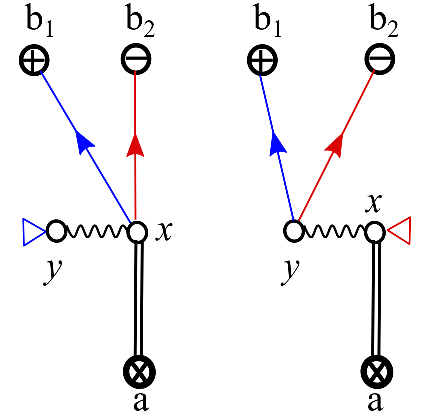
\includegraphics[width=4cm]{Aho2.pdf}} %\includegraphics[width=10cm]{Aho3.png}} 
\ee
%\end{center}
For conciseness, we do not draw the coefficients of these graphs.
%Then we draw some graphs in $\cal A_{ho}^{(3)}$, where each graph in the first line has two light weights and is of fourth order, and each graph in the second line has four solid edges and is of fourth order:
%\begin{center}
%\be  \label{Aho3} 
%\parbox[c]{0.53\linewidth}{\includegraphics[width=\linewidth]{Aho3.png}} 
%\ee
%\end{center}
\end{example}


 
 

To each graph, we assign a value as follows.
  
 \begin{definition}[Values of graphs]\label{ValG} 
For an atomic graph $\mathcal G$, we define its value, denoted by $\llbracket \cal G\rrbracket$, as an expression obtained as follows. We first take the product of 
%all the factors represented by its elements. \cor [ 
all the edges, all the weights and the coefficient of $\cal G$. %when all vertex  labels are given. 
Then for the edges and weights with the same $P_x$ or $Q_x$ label, we group them together and apply $P_x$ or $Q_x$ to them. Finally, we sum over all the internal indices represented by the internal atoms. The values of the external indices are fixed by their given values. 
%If the values for the vertices are not fixed, then the value of the graphs is the sum over all indices represented by the vertices (except for the external vertices $\otimes$, $\oplus$ and $\ominus$). 
 %] \nc 
 For a linear combination of graphs  $\sum_i c_i \cal G_i$, where $\{c_i\}$ is a sequence of coefficients and $\{\cal G_i\}$ is a sequence of graphs, we define  its value by 
 $$ \Big\llbracket\sum_i c_i  \cal G_i\Big\rrbracket=\sum_i c_i \left\llbracket  \cal G_i\right\rrbracket.$$
%We will often  always identify 
For simplicity, we will abuse the notation by identifying  a  graph (which is a geometric object) with its value (which is an analytic expression). 
 \end{definition}
\begin{example}  As an example of Definition \ref{ValG}, we write down the value for the following graph:
  \be\nonumber
 \parbox[c]{0.25\linewidth}{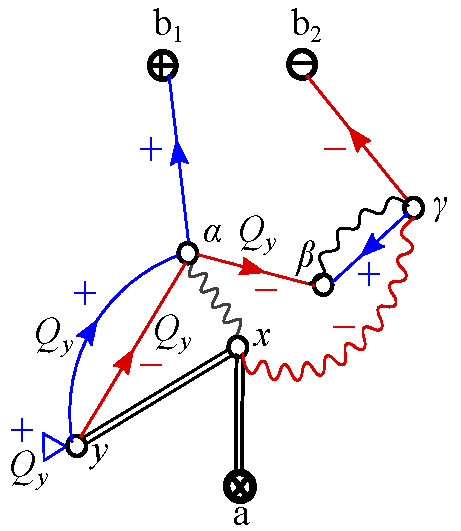
\includegraphics[width=\linewidth]{value_example.pdf}} \quad 
 = \sum_{x,y,\al,\beta,\gamma} \Theta_{\fa x}s_{x\al}S^-_{x\gamma}s_{\beta\gamma}G_{\al\fb_1} G_{\gamma\beta} \overline G_{\gamma\fb_2} \Theta_{xy}Q_y\left[\overline G_{\al\beta}  | G_{y\al }|^2 (G_{yy}-m)\right].
 \ee
\end{example}


\iffalse
All graphs appearing in  this paper  satisfy the properties (i)--(iii) in Definition \ref{defnlvl0}. Moreover, we will always identify pairs of internal atoms that are connected through dotted edges, but we will \emph{not} identify a pair of external and internal atoms because they play very different roles. (We will define the operation of identifying pairs of atoms formally in Definition \ref{def merge} below.) Then after identifying the internal atoms connected through dotted edges, the resulting graphs will also satisfy property (iv) in Definition \ref{defnlvl0}. We call the graphs satisfying these properties (i)--(iv) as \emph{regular graphs}. 
\hty{ here are some confusions. it's best to define regular graphs by introducing   (i)--(iv). Then define the normal regular one and then scaling order. 
otherwise, it is hard to read.  }   However, for a regular graph, its \emph{scaling order} (cf. Definition \ref{def scaling} below) may not be uniquely determined, because a $G$ edge can represent either a diagonal or an off-diagonal $G$ entry. To resolve this issue, we introduce a stronger concept of \emph{normal regular graphs}.
\fi

Next, we introduce the concept of \emph{regular graphs}, which include (almost) all the graphs appearing in this paper, and a stronger concept of \emph{normal regular graphs}.

 \begin{definition}[Normal regular graphs]  \label{defnlvl0} % \cob (need details) \nc 
 We say an atomic graph $\cal G$ is {\bf regular} if it satisfies the following properties:
\begin{itemize}
\item[(i)] it is a connected graph that contains at most $C$ many atoms and edges for a constant $C>0$ (in the $T$-expansion and $\incomp$ below, $C$ is given by the constants $C_n$ and $C_D$ in Definition \ref{defn genuni});
%\item[(ii)] it may have some external atoms whose values are fixed; % (e.g. $\otimes$, $\oplus$ and $\ominus$ atoms are external atoms);
%\item it has no dotted (i.e. $h$) egdes;
%\item[(ii)] each internal atom is connected with an even number of $G$ edges;
\item[(ii)] all the internal atoms are connected together through paths of waved and $\dashed$ edges (these paths may pass through external atoms);
\item[(iii)] there are no dotted edges between internal atoms.
\end{itemize}
 Moreover, we say a regular graph is {\bf normal} if it satisfies the following additional property:
\begin{itemize}
\item[(iv)] every solid edge connects two different atoms (diagonal $G$ factors are represented by weights), and any pair of different atoms $\al$ and $\beta$ in the graph are connected by a $\times$-dotted edge \emph{if and only if} they are connected by a $G$ edge.
\end{itemize}

\iffalse
\begin{itemize}
\item[(v)] for any pair of atoms $\al$ and $\beta$ in the graph, if there are $G$ edges between them, then $\al$ and $\beta$ must  also be connected by a $\times$-dotted edge;

\item[(vi)] %it satisfied the {\bf reverse off-$G$-property}, that is, 
for any pair of atoms $\al$ and $\beta$ in the graph, there is a $\times$-dotted edge between them {\bf only if} there is at least one $G$ edge between them (in other words, if there is no $G$ edge between these two atoms, then they are not connected by a $\times$-dotted edge). 
% for any atoms $\al,\beta$ in the graph, there is a $\times$-dotted edge between them {\bf if} there is at least one $G$ edge between them (\cor every $G$ is associated with $\times$-dotted line\nc); 
 \end{itemize}
 Concisely speaking, every $G$ edge in a normal regular graph  is associated with one $\times$-dotted edge and vice versa. %The collection of level 0 graph contains all graphs appear in this work. 
 
 \hty{ why not say that any two atoms $\al$ and $\beta$ are connected by a  $\times$-dotted edge {\bf if and only if} they are connected by a  $G$ edge? }
 \fi
 \end{definition}



By this definition,  every $G$ edge in a normal regular graph is off-diagonal, while all the diagonal $G$ factors will be represented by weights. There are two reasons for introducing the property (iv): {(1)} in Definition \ref{def scaling}, we need to distinguish between the diagonal and off-diagonal $G$ entries; {(2)} the weight expansion (cf. Definition \ref{Ow-def} below) of diagonal $G$ entries and the edge expansions (cf. Definitions \ref{multi-def}, \ref{GG-def}, \ref{GGbar-def} below) of off-diagonal $G$ entries are very different in nature. 

\iffalse
There are also two reasons for introducing the property (vi). 
\begin{itemize}
\item  There is no need to distinguish between diagonal and off-diagonal waved/$\dashed$ edges. Hence by associating the $\times$-dotted edges with $G$ edges only, we can simplify the graph structures. 

\item We do not want $\times$-dotted edges to appear in deterministic graphs. Because we will need to study the Fourier transforms %(cf. the proof of Lemma \ref{lem FT0}) 
of some deterministic expressions, but the Fourier transform of a $\times$-dotted edge is not well-behaved. 
\end{itemize}
\fi
%Now for a normal regular graph, we can define its scaling order. 

      
   \begin{definition} [Scaling order] \label{def scaling}
   Given a normal regular  graph $\cal G$, we define its scaling order as 
\begin{align}
\text{ord}(\cal G):&= \#\{\text{off-diagonal }  G  \text{ edges}\} + \#\{\text{light weights}\} + 2\#\{ \text{waved edges}\}  + 2 \#\{\text{$\dashed$ edges}\} \nonumber\\
&  - 2\left[ \#\{\text{internal atoms}\}- \#\{\text{dotted edges}\} \right]. \label{eq_deforderrandom2}
\end{align}
Here a dotted edge in a normal regular graph between an internal atom and an external atom means that the internal atom is equal to the external atom, so we lose one free summation index. A dotted edge can also connect two external atoms (e.g., in a diagonal graph of $\Sele_l$ in Definition \ref{collection elements} below), and the number of dotted edges in \eqref{eq_deforderrandom2} counts all dotted edges, including those between external atoms. If the dotted edges contain a cycle, we first remove redundant dotted edges, which does not change the value of the graph, so that in every block of atoms connected by dotted edges, the dotted edges form a spanning tree of this block; in particular, every lost summation index is counted exactly once in \eqref{eq_deforderrandom2}.
%two atoms belong to the same equivalence class if and only if they are connected by a dotted edge (i.e. if and only if they are always equal to each other). 
The concept of scaling order can  be also defined for subgraphs. 
  \end{definition} 
  
%{\cor We define the scaling order of a graph, say $\cal G$, as {\cor (revise this definition)}
%\begin{align}
%\text{ord}(\cal G):&= \#\{\text{solid }  (G - m) \text{ or } (\overline G -\overline m)  \text{ edges}\} + 2\#\{ \text{$S$, $S^{\pm}$, $\Theta$ edges}\}    - 2 \#\{\text{summation indices}\}.\label{eq_deforderrandom0}
%\end{align}
%In mean field model with $L=W$, the scaling order describes the size of the expression in terms of the $W^{-d/2}$ factor, that is, a graph of scaling order $n$ has $\ell^\infty$ norm bounded by $W^{-nd/2}$ (up to a $W^\e$ factor). However, this in general does not hold for band matrices with $L\gg W$, unless the graph satisfies certain structure properties. For a more detailed discussion, we refer the reader to Remark \ref{rmk order} below.
%}
% \begin{remark}
%Since every $G$ edge in a normal regular  graph is off-diagonal, the above definition of order is well-defined. If there is a $G$ edge between two atoms that are connected through a  dotted line, then this $G$ edge becomes a weight on one of the atoms. 
%where $\#_G$ is the total order of all the $G$ edges, defined as following: (i) if there are $G$ edges between two atoms that are connected by a  dashed-dotted edge, then they become weights on one of the atoms and we count their order as 0; (ii) if there are $G$ edges between two atoms that are connected by a $\times$-dashed-dotted edge, then we count their total number as the order; (iii) if there are $G$ edges between two atoms that are neither connected by a $\times$-dashed-dotted edge nor a dashed-dotted edge, then we count their order as $\max(\text{number of these $G$ edges}, 2)$. 
%\end{remark}
%\begin{remark}\label{rmk order}
The motivation behind this definition is as follows. Consider the Wigner ensemble with $W=L$. 
% mean-field case  $W\sim L$ so that all internal indices vary on the scale $L=\OO(W)$. \hty{ I don't understand "indices vary" means?}
%such that there are only local structures in the graph $\cal G$, that is, the internal indices only vary on a scale of order $\OO(W)$ (recall the discussion in Section \ref{sec strategy}). 
By \eqref{subpoly}, \eqref{thetaxy} and \eqref{S+xy}, each waved edge is of order $\OO(W^{-d})$ and each $\dashed$ edge is of order $\OO_\prec(W^{-d})$. %\hty{ it is meaningless to use $\prec$ here. Also, this is about its local size since it is not even summable? } 
Moreover, if we know that $|G_{xy}-m\delta_{xy}|\prec W^{-d/2}$, then each off-diagonal $G$ edge or light weight is bounded by $\OO_\prec(W^{-d/2})$.  Finally, each summation leads to a factor $W^d$. Hence it is easy to obtain the bound %\hty{ do you need doubly connected? } 
$$\llbracket \cal G\rrbracket\prec W^{-\text{ord}(\cal G)\cdot d/2}.$$ 
%\hty{ is $|\cal G|$ the value? But this is not the notation? } 
Later in Lemma \ref{no dot}, %and Lemma \ref{general dot}, 
we will show that this bound holds even if $L\gg W$ as long as the graph satisfies the doubly connected property to be introduced in Section \ref{sec doublenet}. %Intuitively, in a double-net graph, the main contributions of the $G$ edges and $\Theta$ edges come from local scales of order $\OO(W)$, hence the above argument actually makes sense.  
%\end{remark}

  
%For simplicity, 
In the following proof whenever we say the order of a graph, we are referring to its scaling order. We emphasize that in general the scaling order does not imply the ``order of the graph value" directly. 
%---this will be dealt with using the concept of {\bf doubly connected property} in Definition \ref{def 2net}. We refer the reader to Lemmas \ref{no dot} and \ref{general dot} below. 




%where two atoms belong to the same equivalence class if they are connected by a dotted edge. 
%Later we will see that the scaling order describes the scaling of the expression in terms of the $W^{-d/2}$ factor. Roughly speaking, an expression of scaling order $n$ has $\ell^\infty$ norm bounded by $W^{-nd/2}$ (up to a $W^\e$ factor), as long as it satisfies certain structure properties; see Lemma \ref{general dot}. 

\subsection{$\Selfs$}\label{sec self}

The $T$-expansion is defined using a collection of special sums of deterministic graphs, which satisfy some important properties given by Definition \ref{collection elements} below. Following the notations in Feynman diagrams, we call them ``$\selfs$". %In fact, these sums have very similar meaning to the \emph{self-energy} , so we shall call them the ``$\selfs$". 
%Since we will use these properties frequently in this paper, for simplicity of presentation, we introduce the following notion of ``$\selfs$" adopting the language from Feynman diagrams in mathematical physics. %and the corresponding set $\Cele_l$.
As we explained before, %The properties in Definition \ref{collection elements}, especially 
the sum zero property \eqref{3rd_property0} of the $\selfs$ is one of the key reasons why we can define the $T$-expansion up to any order. In previous works \cite{delocal,PartIII}, the $T$-expansion can only be performed to third order without using the concept of $\selfs$.  
 


\begin{definition}[$\Selfs$]\label{collection elements}
Under the assumptions of Theorem \ref{main thm}, for a fixed $l\in \N$, let $\Sele_l(z)\equiv  \Selek_{l}^L(z)$ be a deterministic matrix depending on $m(z)$, $S$, $S^\pm(z)$ and $\Theta(z)$ only, and satisfying the following properties. (In this paper, we will often omit the dependence on $L$ in $\Selek_{l}^L$.)

%let $\Cele_{l}$ be a set of $\OO(1)$ many {\bf deterministic} matrices consisting of $m(z)$, $I_N$, $S$, $S^\pm(z)$ and $\Theta(z)$ only, such that the following properties hold for each $ \Selek_{l} \in \Cele_{l}$ ($\kappa$ labels the expression, $l$ indicates its scaling order, and $\Sele$ is used to mean that they are basic ``elements" in the definition of $T$-expansions).

%For any fixed $l\in \N$, let $\Cele_{l}$ be a set of $\OO(1)$ many {\bf deterministic} matrices consisting of $m(z)$, $I_N$, $S$, $S^\pm(z)$ and $\Theta(z)$ only, such that the following properties hold for each $ \Selek_{l} \in \Cele_{l}$ ($\kappa$ labels the expression, $l$ indicates its scaling order, and $\Sele$ is used to mean that they are basic ``elements" in the definition of $T$-expansions).
 \begin{itemize}
\item[(i)] For any $x,y \in \Z_L^d$, $  (\Selek_{l})_{xy}$ is a sum of at most $C_l$ many deterministic graphs of scaling order $l$ and with external atoms $x$ and $y$. Here $C_l$ is a large constant depending on $l$. These graphs are normal regular, their dotted edges form a forest (i.e., they contain no cycles), and they are doubly connected in the sense of Definition \ref{def 2net} below when $x$ and $y$ are regarded as internal atoms. Some graphs, say $\cal G$, in $\Sele_l$ can be diagonal matrices satisfying $  \cal G_{xy}= \cal G_{xx} \delta_{xy}$, i.e. there is a dotted edge between the atoms $x$ and $y$; these graphs give the second term on the right-hand side of \eqref{4th_property0}. %\hty{ it's not clear you meant that some graph in $\Selek_{l}$ is diagonal or $\Selek_{l}$ itself is diagonal. Your writing suggests the later, but I think it is the former}

\item[(ii)] $ \Selek_{l} (z)$ satisfies the properties \eqref{two_properties0}--\eqref{3rd_property0}.
% \begin{itemize}
% \item[(i)] 
%\hty{ is the sum zero fully stated earlier or we need the following? } 


\item[(iii)]  For any $x,y \in \Z^d$ and $E\in(-2+\kappa,2-\kappa)$, we denote by $(\Seleinf_{l})_{xy}(E)$ the infinite space limit of $\Sele_l$, that is, the sum of the infinite space limits $\cal G^\infty_{xy}$, defined in Definition \ref{def infspace} below, of the graphs $\cal G$ in $\Sele_l$, where the labelled $\dashed$ edges are expanded into $\Theta$ edges and lower order $\selfs$ as in \eqref{defRnl}. In other words, $\Seleinf_l$ is obtained by evaluating the graphs of $\Sele_l$ on $\Z^d$ at $\eta=0$, with $m(E)$, $S_\infty$, $S^\pm_\infty(E)$ and $\Theta_\infty$ in place of $m(z)$, $S$, $S^\pm(z)$ and $\Theta(z)$. It depends only on $E$, $W$ and $\psi$, but not on $L$ and $\eta$, and the estimate \eqref{3rd_property0 diff} below shows that $\Sele_l(z)$ is close to $\Seleinf_l(E)$ when $\eta$ is small.
%Furthermore, the following properties hold $\Selek_{2l}$, $2l\ge 4$:
%% \begin{itemize}
%% \item[(i)] 
% \be\label{two_properties0}
% \Selek_{2l} (x, x+a) =  \Selek_{2l} (0,a), \quad   \Selek_{2l} (0, a) = \Selek_{2l}(0,-a), \quad \forall x,a\in \Z_L^d,
%\ee 
%and for any constant $\e>0$,
%%where we used the notation $R_\Delta^{(2n)} (x, y)\equiv (R_\Delta^{(2n)})_{xy}$; 
%  %\item[(ii)] %From the doubly connected property, we get
%  \be\label{4th_property0}
%W^{ld}\left|  \Selek_{2l} (x,y) \right| \le W^\e \left(W^{-1}\langle x-y\rangle\right)^{-(d+2)}, \quad \forall x,y\in \Z_L^d.
%\ee
%Finally, the infinite space limits of $\Sele_{2l}$ as $L\to \infty$, denoted by $\Seleinf_{2l}:=\lim_{L\to \infty}\Sele_{2l}$, exists. The precise definition of $\Seleinf_{2l}$ will be given in Definition \ref{def infspace}. The limit  $\Seleinf_{2l}$ satisfies the following {\bf sum zero property} for $4\le 2l \le n$, 
%\begin{equation}\label{weaz}
%\sum_y (\Seleinf_{2l})_{xy}=0.
%\end{equation}
%%Similarly, the infinite space limit of $\Sdelta^{(n)}$, $(\Sinfty)^{(n)}:=\sum_{4\le 2l \le n} \Sinfty_{2l}$, also satisfies the sum zero property $ \sum_y (\Sinfty)^{(n)}_{xy}= 0.$
%%satisfy the properties \eqref{two_properties0}, \eqref{4th_property0} and \eqref{3rd_property0}, 
\end{itemize} 
We call $\Selek_l$ the $l$-th order $\self$ ($\Selek_l$ will be unique from our construction) and graphically 
%we will regard each $ (\Selek_{l})_{xy}$ as a single graphical component between atoms $x$ and $y$ and without internal structure. In this paper, for each fixed $l\in \N$, there is only one $l$-th order $\self$. Moreover, 
we will use a square, $\square$, between atoms $x$ and $y$ with a label $l$ to represent $(\Sele_l)_{xy}$. 
\end{definition}
%\begin{remark} {(i)} 

%The precise definition  of $\Seleinf_{l}$ will be given in Definition \ref{def infspace}. \hty{not sure  where and how to say this }

We will show that the infinite space limits of the $\selfs$ satisfy the following properties: 
%\begin{proposition} 
%The limit $(\Seleinf_{l})_{xy}(E)$ exists uniquely and for any small constant $\tau>0$,   $\Seleinf_{l}$ satisfies \cor (\ref{two_properties0}, \ref{4th_property0}) with $ (\Selek^L_{l})_{xy}(z_L)$ replaced by $(\Seleinf_{l})_{xy}(E)$. Furthermore, it satisfies 
%
%that ,  
%\hty{this first one is the same as the earlier one.}
\be\label{two_properties0V}
\Seleinf_{l}(x, x+a) = \Seleinf_{l}(0,a), \quad  \Seleinf_{l}(0, a) =\Seleinf_{l} (0,-a), \quad \forall \ x,a\in \Z^d,
\ee 
%and the following {\bf sum zero property} \nc 
\be\label{4th_property0V}
\left| (\Seleinf_{l})_{0x}(E) \right| \le W^{-ld/2} \frac{W^{2d-4} }{\langle x\rangle^{2d-4-\tau}} + W^{-(l-2)d/2+\tau}\mathbf 1_{x=0}, \quad \forall \ x\in \Z^d,
\ee
\be\label{3rd_property0 diff}
\left| (\Selek^L_{l})_{0x}(z)-(\Seleinf_{l})_{0x}(E) \right| \le W^{-ld/2} \frac{\eta W^{2d-6} }{\langle x\rangle^{2d-6-\tau}} + \eta W^{-(l-2)d/2+\tau}\mathbf 1_{x=0}, \quad \forall \  x\in \Z_L^d \subset \Z^d,\ \eta\in [W^{2}/L^{2-\tau}, L^{-\tau}],
\ee
%and for $4\le 2l \le n$, 
\begin{equation}\label{weaz}
\sum_{x\in \Z^d} (\Seleinf_{l})_{0x}(E)=0.
\end{equation} 
In \eqref{3rd_property0 diff}, with slight abuse of notation, we identify the torus $\Z_L^d$ in \eqref{ZLd} as a subset of $\Z^d$. The properties \eqref{two_properties0V} and \eqref{4th_property0V} take the same forms as the properties \eqref{two_properties0} and \eqref{4th_property0}; as in \eqref{4th_property0}, the terms with $\mathbf 1_{x=0}$ in \eqref{4th_property0V} and \eqref{3rd_property0 diff} come from the diagonal graphs in $\Sele_l$.The property \eqref{weaz} is an exact \emph{sum zero property} and is thus stronger than \eqref{3rd_property0}. 
%\end{proposition} 
These properties will be proved in Lemma \ref{cancellation property}. 

	
By Definition \ref{def scaling}, the scaling order of a deterministic graph can only be even. Moreover, every nontrivial $\self$ $\Selek_{l}$ used in this paper has scaling order $\ge 4$. Hence we always have  %$\Selek_{l}=0$ and 
\be\label{trivial conv}
\Sele_1=\Sele_2=\Sele_3=0, \quad \text{and}\quad \Sele_{2l+1}:=0,\quad l\in \N.
\ee

\iffalse
Moreover, by regarding $ (\Selek_{l})_{xy}$ as a single graphical component of scaling order $\ell$, the Definition \ref{def scaling} can be extended as
\begin{align}
  \text{ord}(\cal G) &= \#\{\text{off-diagonal }  G  \text{ edges}\} + \#\{\text{light weights}\} + 2\#\{ \text{waved edges}\}  + 2 \#\{\text{$\dashed$ edges}\} \nonumber\\
&+\sum_{l} l\cdot  \#\{l\text{-th order $\selfs$}\}    -  2\left[ \#\{\text{internal atoms}\}- \#\{\text{dotted edges}\} \right] , \label{eq_deforderrandom20}
\end{align}
for a normal regular graph $\cal G$. \hty{ this is confusing. you cannot have two definitions of one object}
%{\cob In case the reader is interested, $\kappa$ of $\Selek_k$ actually labels the $\self$ $\Sele_k$ in \eqref{chain S2k}, $\Sele_k$ in \eqref{decompose Sdelta}, and the components in \eqref{Sele gamma}.}
\fi

%\vspace{5pt}
%\noindent{(ii)} 



By property \eqref{two_properties0V}, $\Seleinf_l$ is translationally invariant and symmetric (so are all the deterministic graphs in this paper by Lemma \ref{lem Rsymm}). 
%The first equality in \eqref{two_properties0} means that $\Selek_{l}$ is translation invariant, while the second inequality is equivalent to $\Selek_{l}(0,a)=\Selek_{l}(a,0)$, i.e. $\Selek_{l}$ is symmetric. Similarly, \eqref{two_properties0V} means that $\Seleinf_l$ is translation invariant and symmetric. In this paper, all the deterministic graphs automatically have these properties by Lemma \ref{lem Rsymm}.  \hty{ this and next one seem already said in the intro? Then it should be moved there or we should cite the statement from there. The other properties of this remark were also said in the intro. We should decide what to do to save space and also make ideas apparent. Now there are repetitions. } 
%\vspace{5pt}
%\noindent{(iii)}
The properties \eqref{4th_property0} and \eqref{4th_property0V} show that the rows of $\Selek_{l}$ or $\Seleinf_{l}$ are absolutely summable, i.e.,  
 %. Moreover, combining \eqref{4th_property0} with \eqref{property V-R} below, we get that 
 for any constant $\tau>0$,
 \be\label{sum S2l}\sum_{x}\left| (\Selek_{l})_{0x}  \right| \le W^{-(l-2)d/2 + \tau},\quad \sum_{x}\left| (\Selek_{l}^\infty)_{0x} \right| \le W^{-(l-2)d/2 + \tau} .
 \ee
%\vspace{5pt}\noindent{(iv)} 
The bound \eqref{3rd_property0} is stronger than the first estimate in \eqref{sum S2l} by an extra $\eta$ factor, which, as discussed in Section \ref{sec mainref}, is crucial for our proof.  %implies an intrinsic cancellation inside $\Selek_{l}$. is crucial for our proof as we will explain in Remark \ref{lem redagain} below. 


The property \eqref{3rd_property0 diff} controls the difference between $(\Selek_{l})_{0x}(z)$ and $(\Seleinf_{l})_{0x}(E)$. 
%In particular, for any fixed $x \in \Z_L^d$, the difference converges to 0 when $\eta\to 0$ as $L\to \infty$.
The property \eqref{3rd_property0} actually %is redundant for Definition \ref{collection elements}  in the sense that it
%The property \eqref{3rd_property0} actually 
can be derived from \eqref{4th_property0V}, \eqref{3rd_property0 diff}, and the sum zero property \eqref{weaz} for $\Seleinf_l$.  More precisely, 
\begin{align*}
 \Big|\sum_{x\in \Z_L^d} (\Selek_{l})_{0x}(z)\Big| &=  \Big|\sum_{x\in \Z_L^d} (\Selek_{l})_{0x}(z) - \sum_{x\in \Z^d} (\Seleinf_{l})_{0x}(E)\Big|  \le \sum_{|x|\le L/2} \left| (\Selek_{l})_{0x}(z) -(\Seleinf_{l})_{0x}(E) \right| + \sum_{|x|>L/2}\left|  (\Selek_{l})_{0x}(z) \right| \\
& \le \sum_{|x|\le L/2} W^{-ld/2} \frac{\eta W^{2d-6} }{\langle x\rangle^{2d-6-\tau}} + \eta W^{-(l-2)d/2+\tau} + \sum_{|x|>L/2}W^{-ld/2} \frac{W^{2d-4} }{\langle x\rangle^{2d-4-\tau}} \\
&\lesssim L^\tau \left(\eta+\frac{W^2}{L^2}\right)W^{-(l-2)d/2} \le 2L^\tau \eta W^{-(l-2)d/2},
\end{align*}
where in the first step we used  \eqref{weaz}, in the third step we used \eqref{4th_property0V} and \eqref{3rd_property0 diff}, and in the last step we used $\eta\gg W^2/L^2$. %Hence we will also call \eqref{3rd_property0} a sum zero property.
This gives \eqref{3rd_property0} for $\eta\in [W^{2}/L^{2-\tau}, L^{-\tau}]$. For $\eta\in (L^{-\tau},1]$, \eqref{3rd_property0} follows directly from \eqref{4th_property0}: summing \eqref{4th_property0} over $x$ gives $\big|\sum_{x} (\Selek_{l})_{0x}(z)\big|\le \sum_x |(\Selek_{l})_{0x}(z)| \lesssim L^\tau W^{-(l-2)d/2}\le L^{2\tau}\eta W^{-(l-2)d/2}$, and $\tau>0$ is arbitrary.
 
The $l$-th order $\self$ $\Sele_l$ in this paper is constructed through a specific expansion procedure of the $T$-variables. In general, if a different expansion procedure is used, a different $l$-th order $\self$ may be obtained. Although we expect the $\selfs$ constructed in different procedures to be the same up to negligible errors, this property is not needed in this paper and we will not pursue it. %\hty{ Is it unique? if yes, we should use "the"  } In this paper, for each fixed $l\in \N$, there is only one $l$-th order $\self$. 

 
\iffalse
\vspace{5pt}
\noindent{(v)} Out of the properties %\eqref{two_properties0}--\eqref{3rd_property0} and 
\eqref{two_properties0V}--\eqref{weaz}, the sum zero property \eqref{weaz} is  perhaps the most crucial one. 
%This property is used crucially in bounding the second term of \eqref{mlevelTgdefintro} below. On the other hand, 
A crucial part of this paper is devoted to proving this property for the $\selfs$.  Using Fourier transforms on $\Z^d$, we will show in Lemma \ref{lem FT0} that 
%for any $\Selek_{l}$ appearing in Definition \ref{defn genuni}, 
the scaled sum $W^{(l-2)d/2}\sum_{x}(\Selek_{l})_{0x}$ converges to an integral $\Sint_{l} $ as $L\to \infty$, such that $\Sint_{l} $
%  \cor [this is a terrible notation to use $\mathfrak D_{2l}$ and $\cal D_{2l}$. Also, the limit is taken as $L\infty$?
%  you might use
% \[
%  \cal \cal D_{2l}^L,  \cal \cal D_{2l}^\infty
% \] 
%   ]\nc [\cob $\cal D_{2l}$ is the infinite space limit as $L\to \infty$. I changed it to $\Sinfty$ to indicate this. I changed $\mathfrak D_{2l}$ to $\Sint_{2l}$; may be there is a better choice?\nc]
only depends on $m(E)\equiv m(E+\ii 0_+)$ and the function $\psi$ in Assumption \ref{var profile}, but does not depend on $W$ or $L$. 
In other words, we have that
\be\label{simpleFT} W^{(l-2)d/2}\sum_{x}(\Seleinf_{l})_{0x} = \Sint_{l} \left(m(E),f\right).\ee
Then \eqref{weaz} is equivalent to showing that ${\Sint}_{l} =0$. The above fact is also the main reason why we want to introduce the infinite space limit: in contrast to \eqref{simpleFT}, the Fourier transform of $(\Selek_{l})_{0x}$ on $\Z_L^d$ will depend on $W$ and $L$ in a rather complicated way, which is hard (if possible) to study.\fi
  
%  \iffalse
%  \vspace{5pt}
% \noindent{(vi)} {\cob %As in Feynman diagrams, the graphs in $\Sele_l$ are all \emph{one-particle irreducible graphs}, that is, each of them does not fall into two disconnected pieces if we cut one internal edge in it. This property actually follows from the stronger \emph{double-net property} as given in Definition \ref{def 2net} below. Furthermore, 
% As in Feynman diagrams, the $\self$s represent the corrections to a propagator, and it can be dropped on top of a $\dashed$ edge to give a new type of edges; see Definition \ref{def_graph comp} below. explain the quadratic in $p$ condition}  
% 
%
%Also we make a trivial remark that the row sum ${\Sint}_{l}^{(\kappa)}=0$ does not necessarily mean that the matrix $\Seleinf_{2l}$ itself is $0$.
%As an example, suppose 
%$$ (\Sele_4)_{xy} = s_{xy} \sum_{w} s^2_{xw} - s_{xy}^2.$$
% Then it satisfies \eqref{two_properties0} and \eqref{4th_property0}. Moreover, its infinite space limit as $L\to \infty$ is  (recall \eqref{sxyf})
% $$(\cal E^{\infty}_4)_{xy}=(S_\infty)_{xy}\sum_{w} (S_\infty)^2_{xw} - (S_\infty)_{xy}^2,\quad (S_\infty)_{xy}:=W^{-d}f(|x-y|/W).$$
%  Then $\cal E^{\infty}_4$ is nonzero, but using $\sum_x (S_\infty)_{xy}=1$ we can check that
% $$\sum_x (\cal E^{\infty}_4)_{xy} =\sum_{w} (S_\infty)^2_{xw} -\sum_x (S_\infty)_{xy}^2=0.$$
% \fi
% \end{remark}
%Finally, we remark that the set $\Cele_l$ may change from one line to the next: if we have shown that a new expression satisfies Definition \ref{collection elements} (i)-(iii), then we can regard it as a new element of $\Cele_l$. In the proof, we will state it clearly whenever we want to add a new element to $\Cele_l$.
%\end{remark}
 
\subsection{Definition of the $T$-expansion}\label{sec Texp2}
 
Given $n\in \N$, we will define the $n$-th order $T$-expansion in Definition \ref{defn genuni}, which is an extension of the second order $T$-expansion in \eqref{seconduniversal}. To this end, we first introduce the following two types of graphs. 

\begin{definition}[Recollision graphs and $Q$-graphs]\label{Def_recoll}
%\begin{itemize}

%\item[(I)] 
(i) We say a graph is a $\oplus$/$\ominus$-recollision graph, if there is at least one dotted edge connecting $\oplus$ or $\ominus$ to an internal atom. In other words, a recollision graph represents an expression where we set at least one summation index to be equal to $\fb_1$ or $\fb_2$.

\medskip
\noindent(ii) We say a graph is a $Q$-graph if it contains at least one $Q$ label, and all  $G$ edges and $G$ weights  in the graph (together with all the other random factors that appear in the $Q$-expansions in Section \ref{subsec global}, such as $G^{(x)}$ entries and $(G_{xx})^{-1}$ factors) have the same $Q$ label with a specific atom $x$, i.e., all $Q$ operators are given by the same $Q_x$.
% In other words, a $Q$-graph $\cal G$ represents a fluctuation term, and can be written into one of the following forms depending on whether $x$ is  external  or internal: $\cal G= Q_x(\cal G_x)$, or $\cal G=\sum_x Q_x(\cal G_x)$, where $\cal G_x$ is a graph  with an external atom $x$ and without any $P/Q$ labels. 


%Note that in the latter case $x$ is an internal atom in $\cal G$ because of the sum $\sum_x$.

%\item[(III)] deterministic graphs which have no dash-dotted edges connected with $\otimes$, and are deterministic except for the two $|G_{x\otimes}|^2$ edge connected with $\otimes$. 
%\end{itemize}
\end{definition}

 
We now  define a general $n$-th order $T$-expansion for any fixed $n\in \N$. Besides the properties in Definition \ref{defn genuni}, the graphs in the definition satisfy several additional properties to be stated in Definition \ref{def genuni}. 

\begin{definition} [$n$-th order $T$-expansion]\label{defn genuni}
%For any fixed order $n$, suppose we have defined the sequence of deterministic graphs $S^{(k)}_ \Delta$, $2\le k \le n-1$. Then 
Fix any $n\in \N$ and let $D>n$ be an arbitrary large constant. For $\fa, \fb_1,\fb_2 \in \Z_L^d$, an $n$-th order $T$-expansion of $T_{\fa,\fb_1\fb_2}$ with $D$-th order error is an expression of the following form: %for any fixed large constant $D>0$,  
%\be\label{mlevelTgdefintro}
%T_{xy}= |m|^2  \Theta_{xy} +|m|^2   \left(\Theta \Sdelta^{(n)} \Theta\right)_{xy}  + (\PTn)_{xy} +  (\ATn)_{xy} + (\QTn)_{xy} . %+ \OO_\prec(W^{-D})
%\ee
\be\label{mlevelTgdef}
\begin{split}
T_{\fa,\fb_1 \fb_2}&= m  \Theta_{\fa \fb_1}\overline G_{\fb_1\fb_2} +m   (\Theta \Sdelta^{(n)}\Theta)_{\fa\fb_1} \overline G_{\fb_1\fb_2} \\
&+ (\PTn)_{\fa,\fb_1 \fb_2} +  (\ATn)_{\fa,\fb_1\fb_2}  + (\QTn)_{\fa,\fb_1\fb_2}  +  (\Err_{n,D})_{\fa,\fb_1\fb_2}.
\end{split}
\ee
The graphs on the right side depend only on $n$, $D$, $m(z)$, $S$, $S^{\pm}(z)$, $\Theta(z)$ and $G(z)$, but do not depend on $W$, $L$ and $d$ explicitly. Moreover, they satisfy the following properties with $C_n$ and $C_D$ denoting large constants depending on $n$ and $D$, respectively.
\begin{enumerate}
\item  The graphs on the right side are normal regular graphs (recall Definition \ref{defnlvl0}) with external atoms $\otimes\equiv \fa$, $\oplus\equiv \fb_1$ and $\ominus\equiv \fb_2$, and with at most $C_D$ many atoms.
%Moreover, the expressions on the right-hand side satisfy the following properties.  

\item $\Sdelta^{(n)}$ is a sum of at most $C_n$ many deterministic normal regular graphs. %of $m(z)$, $I_N$, $S$, $S^\pm(z)$ and $\Theta(z)$ only. 
We decompose it according to the scaling order as 
\be\label{decompose Sdelta0} \Sdelta^{(n)} = \sum_{k\le n} \Sdeltak.\ee
%where each $\Sdelta_{k}$ is a sum of deterministic graphs of scaling order $k$. 
Moreover, we have a sequence of $\selfs$ $\Sele_{k}$ satisfying Definition \ref{collection elements} and properties \eqref{two_properties0V}--\eqref{weaz} for $4\le k \le n$ such that $\Sdeltak$ can be written into the following form %of chain structures: 
\be\label{chain S2k}
\Sdeltak=\Sele_{k} + \sum_{ l =2}^k \sum\limits_{ \mathbf k=(k_1,\cdots, k_l) \in \Omega_{k}^{(l)} } \Sele_{k_1}\Theta  \Sele_{k_2}\Theta \cdots \Theta  \Sele_{k_l} . %\mathbf 1\left(\mathbf k \in \Omega_{k}^{(l)}\right).
\ee
%where $\Sele_{k}\in \Cele_{k}$ for $2\le k \le n-1$ and $\Sele_{k_i} \in \Cele_{k_i}$. 
Here all the deterministic graphs with $l=1$ are included into $\Sele_k$ so that the summation starts with $l=2$. Moreover,  $\Omega_{k}^{(l)} \subset \N^l$ is the subset of vectors $\mathbf k$ satisfying that 
\be\label{omegakl}
4\le k_i \le k-1,\quad \text{ and }\quad  \sum_{i=1}^l  k_i  -2(l-1)=k. 
\ee
%$ \Omega_{k}^{(l)} \subset \N^l$ is a subset of vectors such that every $ \mathbf k \in \Omega_{k}^{(l)} $ satisfies %\eqref{omegakl},  
%\be\label{omegakl}
% 4\le k_i \le k-1,\quad \text{ and }\quad \left(\sum_{i=1}^l  k_i\right) -2(l-1)=k, 
% \ee
The second condition in \eqref{omegakl} guarantees that the subgraph $(\Sele_{k_1}\Theta  \Sele_{k_2}\Theta \cdots \Theta  \Sele_{k_l})_{xy}$ has scaling order $k$.
%But we remark that $ \Omega_{k}^{(l)}$ does not necessarily contain all possible vectors $\mathbf k\in \N^l$ that satisfy \eqref{omegakl}.
%${\bm \kappa}=(\kappa_1,\cdots, \kappa_l)$ is a sequence of labels for the expressions $\Sele_{k_i}$, $1\le i \le l$ (as an additional remark, $\kappa_i$ does not necessarily range over all the elements in $\Cele_{k_i}$). 
%Finally, the deterministic expression $\Sele_{n}$ satisfies the properties (i)-(iii) of Definition \ref{collection elements}.  %and we include it into the set $\Cele_n$.  
%for each fixed $l\in \N$, there are at most $C_l$ many labels $\kappa$ for $\Selek_{2l}$, and as a convention, we regard the label of $\Sele_{2k}$ as $\emptyset$.
 
 
\item $(\PTn)_{\fa,\fb_1\fb_2}$ is a sum of at most $C_n$ many $\oplus/\ominus$-recollision graphs of scaling order $\le n$ and without any $P/Q$ labels.  Moreover, it can be decomposed as 
 \be\label{decomposeP}(\PTn)_{\fa,\fb_1\fb_2} =\sum_{ k =3}^{ n}(\PTk)_{\fa,\fb_1\fb_2},\ee
 where each $(\PTk)_{\fa,\fb_1\fb_2}$ is a sum of the $\oplus/\ominus$-recollision graphs of scaling order $k$ in $(\PTn)_{\fa,\fb_1\fb_2}$. 


\item  $(\ATn)_{\fa,\fb_1\fb_2}$ is a sum of at most $C_D$ many graphs of scaling order $> n$ and without any  $P/Q$ labels.  


\item $(\QTn)_{\fa,\fb_1\fb_2} $ is a sum of at most $C_D$ many $Q$-graphs.  Moreover, it can be decomposed as 
\be\label{decomposeQ} (\QTn)_{\fa,\fb_1\fb_2}= \sum_{k=2}^{n} (\QTk)_{\fa,\fb_1\fb_2} + (\cal Q^{(>n)}_T)_{\fa,\fb_1\fb_2},\ee
where  $(\QTk)_{\fa,\fb_1\fb_2}$ is a sum of the scaling order $k$ $Q$-graphs in $ (\QTn)_{\fa,\fb_1\fb_2}$ and $(\cal Q^{(>n)}_T)_{\fa,\fb_1\fb_2}$ is a sum of all the scaling order $>n$ $Q$-graphs in $ (\QTn)_{\fa,\fb_1\fb_2}$.



\item $\Sdeltak$, $\PTk$ and $\QTk$ are independent  of $n$.

\item $(\Err_{n,D})_{\fa,\fb_1\fb_2}$ is a sum of at most $C_D$ many graphs, each of which has scaling order $> D$ and may contain some $P/Q$ labels in it. 

\item In each graph of $(\PTn)_{\fa,\fb_1\fb_2}$, $(\ATn)_{\fa,\fb_1\fb_2}$, $(\QTn)_{\fa,\fb_1\fb_2} $ and $(\Err_{n,D})_{\fa,\fb_1\fb_2}$,  there is a unique  $\dashed$ edge connected to $\otimes$. Furthermore,  there is at least an edge, which is either  plus solid $G$ or $\dashed$ or dotted,  connected to  $\oplus$, 
 and  there is at least an edge, which is either  minus solid $G$ or $\dashed$ or dotted,  connected to $\ominus$.
 
 %Furthermore, there may be some dotted edges connected with $\oplus$ and $\ominus$. 

%\iffalse
%\item $(\PTn)_{xy}$ is a sum of at most $C_n$ many recollision graphs of scaling order $\le n$: 
% $$(\PTn)_{xy} =\sum_{k=3}^{ n}(\PTk)_{xy},$$
% where each $(\PTk)_{xy}$ is a sum of recollision graphs of scaling order $k$. Here a recollision graph means that there is at least one dotted edge connecting the external vertex $y$ to an internal vertex in the graph. In other words, a recollision graph represents an expression where we set at least one summation index to be equal to $y$.
% %some summation indices in the expression of $(\PT_l)_{xy}$ are equal to the fixed indices $x$ or $y$ {\cor(check this sentence)}.
%\item $(\ATn)_{xy}$ is a sum of at most $C_n$ many higher order graphs with scaling order $> n$. 
%
%\item $(\QTn)_{xy}$ is a sum of at most $C_n$ many $Q$-graphs. Here a $Q$-graph means a fluctuation expression of the form $\sum_\al Q_\al (\Gamma(\al))$ for a graph $\Gamma$ and an internal vertex $\al$ in $\Gamma$, where we denote $Q_\al:=1-\mathbb E_\al$ with $\E_\al[\cdot]$ being the partial expectation over the $\al$-th row and column of $H$.
%Moreover, we can write %decompose $\QTn$ as 
%$$ (\QTn)_{xy}= \sum_{k=2}^{n} (\QTk)_{xy} + (\cal Q^{(>n)}_T)_{xy},$$
%where each $(\QTk)_{xy}$ is the sum of $Q$-graphs of scaling order $k$ in $(\QTn)_{xy}$, and $(\cal Q_T^{(>n)})_{xy}$ is the sum of all the $Q$-graphs of scaling order $>n$ in $(\QTn)_{xy}$.
% \fi
 
\end{enumerate}
The graphs on the right-hand side of \eqref{mlevelTgdef} satisfy some additional properties, which will be given in Definition \ref{def genuni} below. %and Definition \ref{def genuni2}.
\end{definition}



%\begin{remark}\label{lem redagain}
%We make the following remarks regarding Definition \ref{defn genuni}.

%\vspace{5pt}\noindent{(i)} 

In accordance with \eqref{trivial conv}, we have that
$$\Sigma_{T,1}=\Sigma_{T,2}=\Sigma_{T,3}=\Sigma_{T,2l+1}=0,\quad l\in \N.$$
% \end{remark}
% \begin{remark}
%
%Compared with \eqref{sum S2l}, the estimate \eqref{3rd_property0} is much stronger by an extra $\eta$ factor, which actually follows from the sum zero property \eqref{weaz} and is crucial for our proof. In particular, 
%Using \eqref{3rd_property0}, 
With \eqref{label_Theta}, we can bound $\left(\Theta \Sdeltak \Theta\right)_{\fa\fb_1}$ by % in \eqref{intro_redagain}. 
\be\label{intro_redagain}\left(\Theta \Sdeltak \Theta\right)_{\fa\fb_1} \prec W^{-(k-2)d/2}B_{\fa\fb_1}. \ee
%for any constant $\tau>0$. 
%Note that $\left(\Theta \Sdelta_{k} \Theta\right)_{xy}$ satisfies the same bound as $\Theta$ in \eqref{thetaxy} but with an extra $W^{-(k/2-1)d}$ scaling factor (recall that $\Theta_{xy}$ has scaling order $2$, while $\left(\Theta \Sdelta_{k} \Theta\right)_{xy}$ has scaling order $k$). Since $\left(\Theta \Sdelta_{2k} \Theta\right)_{xy} $ is a deterministic term in the $T$-expansion \eqref{mlevelTgdefintro}, 
This bound shows that when $\fb_1=\fb_2=\fb$, the second term on the right-hand side of \eqref{mlevelTgdef} can be bounded by  \smash{$m\overline G_{\fb\fb}(\Theta \Sdelta^{(n)} \Theta)_{\fa\fb}\prec B_{\fa\fb}$}, which is necessary for \eqref{locallaw} to hold.
%Notice that summing over \eqref{4th_property0} we can only get 
%$$\sum_{x}  \Big|S_{\Delta}^{(n)}(x,y)\Big|  \prec W^{-d}.$$
%Compared with this estimate, \eqref{3rd_property0} gains an extra factor $\eta$. This extra factor is crucial for our proof, 
%, showing that there is an inherent cancellation within $S_{\Delta}^{(n)}(x,y)$. Hence we shall call \eqref{3rd_property0} the {\bf cancellation property}, which is one of the most key point of our proof. 
%If \eqref{two_properties0}, \eqref{4th_property0} and \eqref{3rd_property0} hold for $\Sdelta_{2l}$,  then 
%Under the assumptions of Lemma \ref{lem V-R}, 
%For $\Sigma_{2k}$ in Definition \ref{defn genuni}, we have that for any constant $\e>0$,
%Hence it guarantees that the second term on the right-hand side of \eqref{mlevelTgdefintro} has the correct size $B_{xy}$.   
%\end{lemma}
%\begin{proof}
The rigorous proof of \eqref{intro_redagain} will be given in Lemma \ref{lem redundantagain}. 
When $\fb_1=\fb_2= \fb$, by \eqref{Aho>2} the two graphs in $(\cal R_{T,3})_{\fa,\fb\fb}$ are 
$$ m\sum_{x,y}\delta_{x \fb} \Theta_{\fa x} s_{xy} (G_{yy}-m) |G_{x \fb}|^2  + m \sum_{x,y}\delta_{y \fb} \Theta_{\fa x} s_{xy}  ( \overline G_{xx} - \overline m) |G_{y \fb}|^2,$$
which can be easily bounded by $\Theta_{\fa\fb}\prec B_{\fa\fb}$. %if we have a rough estimate $\max_x |G_{xx}|=\OO_\prec(1)$ on the diagonal entries. 
In general, there are many more complicated graphs in \smash{$(\PTn)_{\fa,\fb_1 \fb_2}$}, but they all satisfy good enough bounds for our prupose. 
% \end{remark}
% \begin{remark}
% \vspace{5pt}
%\noindent{(iv)} 
If $D>0$ is sufficiently large, the term $(\Err_{n,D})_{\fa,\fb_1\fb_2}$ will be negligible for all proofs. If a graph in $(\Err_{n,D})_{\fa,\fb_1\fb_2}$ does not contain any  $P/Q$ label, then it can  be also included into {$(\ATn)_{\fa,\fb_1\fb_2}$}.

\iffalse
In the proof of Lemma \ref{lem redundantagain}, the $\eta$ factor in \eqref{3rd_property0} plays an essential role in the sense that it will cancel the following factor from the row sums of $\Theta$:
\be\nonumber %\label{sumTheta}
\sum_{y}\Theta_{xy}(z)=\frac{|m(z)|^2 }{1-|m(z)|^2 }\sim \eta^{-1}.
\ee
%The estimate \eqref{intro_redagain} explains why the sum zero property \eqref{3rd_property0}, as a consequence of \eqref{weaz}, is so important for our proof. 

%\vspace{5pt}
\noindent{(ii)} We now give a more intuitive explanation of why \eqref{intro_redagain} holds. Suppose $\Sele(x)$ is a symmetric function on $\Z_L^d$ with support in $[-CW,CW]^d$, and satisfies that $\|\Sele(x)\|=\OO(W^{-d})$ and $\sum_x \Sele(x)=0$. Then for the function $B(x):=B_{0x}$, with Taylor expansion we get that 
\begin{align*}
\sum_{y:|y-x| \le CW}B(y) \Sele(y-x) &=B(x) \sum_y  \Sele(y-x)  + B'(x) \sum_y  (y-x)\Sele(y-x) + \frac{1}{2}\sum_y B''(\zeta_y)\Sele(y-x) \\
&= \frac{1}{2}\sum_y B''(\zeta_y)\Sele(y-x),
\end{align*} 
\hty{ again, this is repetition} 
where $\zeta_y$ is a point inside $x+[-CW,CW]^d$, and in the second step the first two terms vanish because of the sum zero property and the symmetry of $\Sele$. It is easy to see that $B''(\zeta_y)\prec \langle x\rangle^{-d}$, where $\langle x\rangle^{-d}$ is now a summable function on $\Z_L^d$ (up to a factor $\log L$). With this estimate, we immediately get that 
$$\sum_{ x_1,x_2,\cdots, x_{2k}}\left[\prod_{i=1}^k B_{x_{2i-1} x_{2i}}\Sele(x_{2i+1}-x_{2i})\right] \cdot B_{x_{2k}y}  \prec B_{x_1 y}.$$
This argument can be extended to the proof of \eqref{intro_redagain} because: (1) $\Theta_{0x}$ is also a slow-varying function on the scale $\langle x\rangle$, so that its second derivative is bounded by $\langle x\rangle^{-d}$; (2) although $(\Sele_k)_{0y}$ is not compactly supported as a function of $y$, its behavior is dominated by the region with $y\in [-W^{1+\e},W^{1+\e}]^d$ by \eqref{4th_property0}; (3) although $\sum_y (\Sele_k)_{0y}$ is not exactly zero, the $\eta$ factor in \eqref{3rd_property0} is enough to cancel the $\eta^{-1}$ factor in \eqref{sumTheta}.
\fi 


In Section \ref{sec_basiclocal}, we will describe the basic graph operations that are used to obtain the $T$-expansion, and more details will  be given in \cite{PartII_high}. Assuming the $n$-th order $T$-expansion, we can prove Theorem \ref{main thm}. % for a random band matrix with $L$ satisfying the condition \eqref{Lcondition0} below. 
 
\begin{theorem}\label{thm ptree}
Fix any $n\in \N$. Suppose the assumptions of Theorem \ref{main thm} hold, and we have an $n$-th order $T$-expansion given in Definition \ref{defn genuni} (together with the additional properties in Definition \ref{def genuni}). 
%Suppose for all $2l\le k \le n-1$, properties \eqref{two_properties0R}-\eqref{3rd_property0R} hold for $R_{2l}^{(k)}$. 
Assume that $L$ satisfies 
\be\label{Lcondition1}  {L^2}/{W^2}  \le W^{(n-1)d/2-c_0} \ee
for some constant $c_0>0$. Then for any constant $\e>0$, the local law %\eqref{locallaw} 
\be\label{locallaw1}
|G_{xy} (z) -m(z)\delta_{xy}|^2 \prec B_{xy}
\ee
holds uniformly in all $z= E+\ii\eta$ with $E\in (-2+\kappa,2-\kappa)$ and $\eta \in [W^{2}/L^{2-\e},1]$.
\end{theorem}

%\begin{lemma}
% {\cor add results on $T$-estimates}
%\end{lemma}


If we have obtained the $n$-th order $T$-expansion for $n= n_{W,L}:= \left\lceil\frac{4}{d}\left(\log_W L  - 1 + \frac{c_0}{2}\right)\right\rceil+1$, then we can conclude Theorem \ref{main thm} by using Theorem \ref{thm ptree}. Although $n_{W,L}$ depends on $W$ and $L$, it is bounded by a constant: since $L\le W^{1/c_1}$ under the assumptions of Theorem \ref{main thm}, we have $n_{W,L}\le n_*:=\left\lceil\frac{4}{d}\left(\frac{1}{c_1}  - 1 + \frac{c_0}{2}\right)\right\rceil+2$. Hence it suffices to construct the $T$-expansions up to the fixed order $n_*$, which depends only on $d$, $c_0$ and $c_1$. Theorem \ref{thm ptree} is Theorem 3.6 of \cite{PartII_high}, and its proof is given in Section 7 of \cite{PartII_high}; see Section \ref{sec pfmain} for how it is used.



%The reason why we have assumed an $(n-1)$-th order $T$-expansion instead of an $n$-th order $T$-expansion is as follows. In the proof of Theorem \ref{main thm}, we will use an induction argument on the order of the $T$-expansion. For the induction hypothesis, we assume that we have constructed the $(n-1)$-th order $T$-expansion. Then with Theorem \ref{thm ptree}, we can obtain a local law for random band matrices satisfying \eqref{Lcondition0}. %This result will be used to prove the sum zero properties of the $n$-th $\self$ $\Sele_n$, which completes the construction of the $n$-th order $T$-expansion. 
%For the details of how the $T$-expansions and Theorem \ref{thm ptree} are used in the proof of Theorem \ref{main thm}, we refer the reader to Section \ref{sec pfmain}. 
 

\subsection{Definition of the $\Incomp$}

%{\cor restart here}
In this subsection, we define the concept of \emph{$\incomp$}. 

\begin{definition} [$n$-th order $\incomp$]\label{defn incompgenuni}
	%For any fixed order $n$, suppose we have defined the sequence of deterministic graphs $S^{(k)}_ \Delta$, $2\le k \le n-1$. Then 
Fix any $n\in \N$ and let $D>0$ be an arbitrary large constant. For $\fa, \fb_1,\fb_2 \in \Z_L^d$, an $n$-th order $\incomp$ of $T_{\fa,\fb_1\fb_2}$ with $D$-th order error is an expression of the following form: %for any fixed large constant $D>0$,  
	%\be\label{mlevelTgdefintro}
	%T_{xy}= |m|^2  \Theta_{xy} +|m|^2   \left(\Theta \Sdelta^{(n)} \Theta\right)_{xy}  + (\PTn)_{xy} +  (\ATn)_{xy} + (\QTn)_{xy} . %+ \OO_\prec(W^{-D})
	%\ee
	\be \label{mlevelT incomplete}
	\begin{split}
		T_{\fa,\fb_1 \fb_2} &= m  \Theta_{\fa \fb_1}\overline G_{\fb_1\fb_2}   +\sum_x (\Theta \wtSdeltan)_{\fa x} T_{x,\fb_1\fb_2} \\
		&+ (\PITn)_{\fa,\fb_1 \fb_2} +  (\AITn)_{\fa,\fb_1 \fb_2} + (\QITn)_{\fa,\fb_1 \fb_2} + (\Err'_{n,D})_{\fa,\fb_1\fb_2}  ,
	\end{split}
	\ee
	where the graphs on the right-hand side depend only on $n$, $D$, $m(z)$, $S$, $S^{\pm}(z)$, $\Theta(z)$ and $G(z)$, but do not depend on $W$, $L$ and $d$ explicitly. %(Here ``$IT$" in the subscript means ``initial $T$-expansion".) 
	Moreover, they satisfy the following properties.
	\begin{enumerate}
		\item  $(\PITn)_{\fa,\fb_1 \fb_2}$, $(\AITn)_{\fa,\fb_1 \fb_2}$, $(\QITn)_{\fa,\fb_1 \fb_2}$ and $(\Err'_{n,D})_{\fa,\fb_1\fb_2}$ respectively satisfy the same properties as $(\PTn)_{\fa,\fb_1 \fb_2}$, $(\ATn)_{\fa,\fb_1 \fb_2}$, $(\QTn)_{\fa,\fb_1 \fb_2}$ and $(\Err_{n,D})_{\fa,\fb_1\fb_2}$ in Definition \ref{defn genuni}. Furthermore,  $(\PITn)_{\fa,\fb_1 \fb_2}$ and $(\QITn)_{\fa,\fb_1 \fb_2}$ can be decomposed as
		\be\label{decomposePIT}(\PITn)_{\fa,\fb_1\fb_2} =\sum_{ k =3}^{ n}(\PITk)_{\fa,\fb_1\fb_2},\ee
		and
		\be\label{decomposeQIT} (\QITn)_{\fa,\fb_1\fb_2}= \sum_{k=2}^{n} (\QITk)_{\fa,\fb_1\fb_2} + (\cal Q^{(>n)}_{IT})_{\fa,\fb_1\fb_2},\ee
		where  $(\PITk)_{\fa,\fb_1\fb_2}$ is a sum of the scaling order $k$ $\oplus/\ominus$-recollision graphs in $(\PITn)_{\fa,\fb_1\fb_2}$,  $(\QITk)_{\fa,\fb_1\fb_2}$ is a sum of the scaling order $k$ $Q$-graphs in $(\QITn)_{\fa,\fb_1 \fb_2}$, and $(\cal Q^{(>n)}_{IT})_{\fa,\fb_1\fb_2}$ is a sum of the scaling order $>n$ $Q$-graphs in  $(\QITn)_{\fa,\fb_1\fb_2}$.  Moreover, $\PITk$ and $\QITk$ are independent of $n$.
		% i.e. they are the same expressions in every order $\incomp$.
		
		\item $\wtSdeltan$ %is a sum of at most $C_n$ many deterministic normal regular graphs, where $C_n$ is a large constant depending on $n$. Moreover, it 
		can be decomposed according to the scaling order as 
		\be\label{decompose Sdelta} 
		\wtSdeltan = \Sele_n + \sum_{l=4}^{n-1} \Sele_{l},
		\ee
		where $\Sele_{l}$, $1\le l \le n-1$, is a sequence of $\selfs$ satisfying Definition \ref{collection elements} and properties \eqref{two_properties0V}--\eqref{weaz}. For any $x,y \in \Z_L^d$, $(\Sele_{n})_{xy}$ is a sum of at most $C_n$ many deterministic graphs of scaling order $n$ and with external atoms $x$ and $y$. 
		%Moreover, it has an infinite space limit $\Sele^{\infty}_{n}(E)$ as $L\to \infty$, and satisfies the properties \eqref{two_properties0}, \eqref{4th_property0}, \eqref{two_properties0V} and \eqref{4th_property0V} with $l=n$. 
		
		\item Each graph of $(\PITn)_{\fa,\fb_1\fb_2}$, $(\AITn)_{\fa,\fb_1\fb_2}$, $(\QITn)_{\fa,\fb_1\fb_2} $ and $(\Err_{n,D}')_{\fa,\fb_1\fb_2}$ can be written into %the following form:
		$$ \sum_{x}\Theta_{\fa x} {\cal G}_{x,\fb_1\fb_2},$$ 
		where $ {\cal G}_{x,\fb_1\fb_2}$ is a normal regular graph with external atoms $x$, $\fb_1$ and $\fb_2$. Moreover, $ {\cal G}_{x,\fb_1\fb_2}$ has at least an edge, which is either plus solid $G$ or $\dashed$ or dotted,  connected to  $\oplus$, and at least an edge, which is either minus solid $G$ or $\dashed$ or dotted, connected to $\ominus$.
		
		 %it has one plus solid $G$ or $\dashed$ or dotted edge connected with $\oplus$, and one minus solid $ G$ or $\dashed$ or dotted edge connected with $\ominus$.
	
		 %there is at least an edge, which is either  plus solid $G$ or $\dashed$ or dotted,  connected to  $\oplus$, 	and  there is at least an edge, which is either  minus solid $G$ or $\dashed$ or dotted,  connected to $\ominus$.
	\end{enumerate}
	The graphs on the right side of \eqref{mlevelT incomplete} satisfy some additional properties, which will be given in Definition \ref{def incompgenuni} below.
\end{definition} 
%\begin{remark}
%	We make the following remarks regarding the above definition. 
%	\vspace{5pt}
%	\noindent{(i)} 
The form of \eqref{mlevelT incomplete} is different from \eqref{mlevelTgdef} only in the second term on the right-hand side. We can regard \eqref{mlevelT incomplete} as a linear equation of the $T$-variable $T_{x,\fb_1\fb_2}$. % in the second term on the right-hand side has not been expanded yet. 
In fact, taking $\fb_1=\fb_2$ and $n=M$ in \eqref{mlevelT incomplete}, if we move the second term on the right-hand side to the left-hand side, multiply both sides by $(1-\Theta\wtSdeltan)^{-1}$ and take expectation, then we will get \eqref{E_locallaw}. More details of the proof %of Theorem \ref{main thm2} 
will be given in Section \ref{sec pf0}.
%	\vspace{5pt}
%	\noindent{(ii)}


The $\Sele_l$'s in \eqref{decompose Sdelta} are the same $\selfs$ as in Definition \ref{defn genuni}. 
We remark that the sequence of $\incomp$s is constructed inductively. In particular, before constructing the $n$-th order $\incomp$, we have obtained the $k$-th order $\incomp$ and proved the properties \eqref{two_properties0}--\eqref{3rd_property0} and \eqref{two_properties0V}--\eqref{weaz} for $\Sele_k$ for all $4\le k\le n-1$. On the other hand, $ \Sele_n$ is a new sum of deterministic graphs obtained in the $n$-th order $\incomp$, whose properties \eqref{two_properties0}--\eqref{3rd_property0} and \eqref{two_properties0V}--\eqref{weaz} are yet to be shown.  %\hty{some eq numbers with 0V were changed}
	


%\section{Graphical tools}

\section{Basic graph operations}\label{sec_basiclocal}


%In this section, we discuss the basic graph operations that are used to get the $T$-expansions. The full construction of the $T$-expansions will be discussed in more details in \cite{PartII_high}. %We perform the graph expansions using graph operators. 
%To organize the graph expansions, we will define several graph operators. 
%Recall Definition \ref{ValG} that  %Given a graph $\cal G$ and
A graph operation $\cal O[\cal G]$ on a graph $\cal G$ is a linear combination of new graphs such that the graph value of  $\cal G$ 
is unchanged, i.e. $\llbracket \cal O[\cal G]\rrbracket=\llbracket \cal G\rrbracket$. 
%Hence a graph operator acting on a graph represents both a graph expansion, where an old graph is expanded into the sum of several new graphs, and a mathematical identity in the sense of graph values. 
All graph operations are linear, that is, %that is, for a linear combination of graphs  $\sum_i c_i \cal G_i$, where $\{c_i\}$ is a sequence of   coefficients and $\cal G_i$ is a sequence of graphs, we have 
%so that 
\be\label{linear graphO} \cal O\Big[\sum_i c_i  \cal G_i\Big] =\sum_i c_i \cal O\left[ \cal G_i\right].
\ee

\subsection{Dotted edge operations} 
% In this subsection, we define two graph operators related to dotted edges---$\cal O_{merge}$ in Definition \ref{def merge} and $\cal O_{dot}$ in Definition \ref{dot-def}. 

Recall that a dotted edge between atoms $\al$ and $\beta$ represents a $\delta_{\al\beta}$ factor. We will identify  internal atoms  connected by dotted edges, but we will {\it not} identify an external and an internal atom due to their different roles in graphs. Dotted edges between internal atoms may appear in intermediate steps, so we define the following merging operation. 
\begin{definition}[Merging operation]\label{def merge}
Given a graph $\cal G$ that contains dotted edges between different atoms, we define an operator $\cal O_{merge}$ in the following way: $\cal O_{merge}[\cal G]$ is a graph obtained by merging every pair of internal atoms, say $\al$ and $\beta$, that are connected by a path of dotted edges into a single internal atom, say $\gamma$. Moreover, the weights and edges attached to $\al$ and $\beta$ %in $\cal G$ 
are now attached to the atom $\gamma$ 
 in $\cal O_{merge}[\cal G]$. In particular, the $G$ edges between $\al$ and $\beta$ become weights on $\gamma$, and the waved and $\dashed$ edges between $\al$ and $\beta$ become self-loops on $\gamma$. If $\al$ and $\beta$ are both connected to the same external atom by dotted edges, then $\gamma$ is connected to this external atom by one dotted edge. In general, after the merging we remove redundant dotted edges, which does not change the graph value, so that in every block of atoms connected by dotted edges, the dotted edges form a spanning tree of this block; in particular, every lost summation index is counted exactly once in \eqref{eq_deforderrandom2}.
\end{definition}
%\begin{remark}
It is easy to see that the graph operator $\cal O_{merge}$ is an identity in the sense of graph values:
 $ \llbracket \cal O_{merge}[\cal G]\rrbracket=\llbracket \cal G\rrbracket$.
%We  stress  that a path of dotted edges can pass through an external atom, but we will not identify the internal atoms on this path with the external atom.  \hty{We  stress  that  we will not identify  internal atoms which are connected by dotted edges only through an external atom.}
%\end{remark}
Given any regular graph, we can rewrite it as a linear combination of normal regular graphs %satisfying property (v) of Definition \ref{defnlvl0} 
using the following \emph{dotted edge partition} operation. 

%\iffalse
%More precisely, if $\cal G$ does not satisfy the {off-$G$-property}, then we first assign the following {\bf dotted-line partition} of all the pairs of atoms that are connected by a $G$ edge. In other words, given two atoms $\al$ and $\beta$, if there are $G$ edges between them, then we decompose 
%\be\label{assigndot}1= \mathbf 1_{\al\ne \beta} + \mathbf 1_{\al = \beta}. \ee
%If there is a $\times$-dotted line between $\al$ and $\beta$, then the edges between them are all off-diagonal; otherwise, all the edges become weights on $\al$ or $\beta$. In this way, we can write %a graph $\cal G$ as 
%$$\left\llbracket \cal G \right\rrbracket= \sum \left\llbracket \cal O_{merge}[{Dot} \cdot \cal G ]\right\rrbracket,$$
%where each ${Dot}$ is a product of some dotted and $\times$-dotted edges such that each ${Dot} \cdot \cal G$ satisfies the {off-$G$-property}. Here the sum is over all possible self-consistent ${Dot}$, where the {\bf self-consistency} means: if $x_i$ and $x_j$ are connected by a dotted edge in ${Dot}$, and $x_j$ and $x_l$ are also connected by a dotted edge in ${Dot}$, then $x_i$ and $x_l$ {\bf cannot} be connected by a $\times$-dotted edge in ${Dot}$. The operator $\cal O_{merge}$ merges all pairs of internal atoms in ${Dot} \cdot \cal G$ connected by a dotted edge.
%  \fi

\begin{definition}[Dotted edge partition] \label{dot-def}
 %{\bf Assigning dotted-line partition $\cal O_{dot}$:} 
 Given a regular graph $\cal G$, for any pair of atoms $\al$ and $\beta$, if there is at least one $G$ edge but no $\times$-dotted edge between them, then we write 
 $$1=\mathbf 1_{\al=\beta} + \mathbf 1_{\al \ne \beta} ;$$
  if there is a $\times$-dotted line $ \mathbf 1_{\al\ne \beta}$ but no $G$ edge between them, then we write 
 $$\mathbf 1_{\al\ne \beta} =1 - \mathbf 1_{\al = \beta}.$$
 Expanding the product of all these sums on the right-hand sides, we can expand $\cal G$ as
 \be\label{odot}\cal O_{dot}[\cal G] := \sum \cal O_{merge}[{\Dot} \cdot \cal G],\ee
 where each ${\Dot}$ is a product of dotted and $\times$-dotted edges together with a $+$ or $-$ sign. %such that $\cal O_{merge}[{\Dot} \cdot \cal G]$ is a normal regular graph.
  In ${\Dot} \cdot \cal G$, if there is a $\times$-dotted edge between $\al$ and $\beta$, then the $G$ edges between them are off-diagonal; otherwise, the $G$ edges between them become weights after the merging operation. (If $\al$ and $\beta$ are connected by a path of dotted edges but are not merged because at least one of them is an external atom, then a $G$ edge $G_{\al\beta}$ or $\overline G_{\al\beta}$ between them is regarded as the weight $G_{\al\al}$ or $\overline G_{\al\al}$ on its first atom $\al$.) If $\Dot$ is ``inconsistent" (i.e., two atoms are connected by a  $\times$-dotted edge and a path of dotted edges), then we trivially have $\llbracket \Dot \cdot \cal G\rrbracket=0$. Thus we will drop all inconsistent graphs.  Finally, if the graph $\cal G$ is already normal, then $\cal O_{dot}$ acting on $\cal G$ is a null operation and we let $\cal O_{dot}[\cal G]:=\cal G$.
  
  \iffalse
  Without loss of generality, we only sum over consistent  ${\Dot}$s, that is, if $x_i$ and $x_j$ are connected by a dotted edge in ${\Dot}$, and $x_j$ and $x_k$ are connected by a dotted edge in ${\Dot}$, then $x_i$ and $x_k$  cannot be connected by a $\times$-dotted edge in ${\Dot}$. Note that if $\Dot$ is not self-consistent, then we trivially have $\llbracket \Dot \cdot \cal G\rrbracket=0$.
  \fi
  
 
 
% \medskip
%\noindent  {\bf Removing $\times$-dotted lines $\cal O_{rDot}$:} 
%  Given a regular graph $\cal G$, for any pair of atoms $\al$ and $\beta$, if there is a $\times$-dotted line $ \mathbf 1_{\al\ne \beta}$ and but {\bf no} $G$ edge between them, then we write 
% $$\mathbf 1_{\al\ne \beta} =1 - \mathbf 1_{\al = \beta}.$$
% Expanding the product of all these sums, we can expand $\cal G$ as
% \be\label{ordot}\cal O_{rDot}(\cal G)= \sum \cal O_{merge}[\rDot \cdot \cal G],\ee
% where each ${\rDot}$ is a self-consistent product of dotted and $\times$-dotted edges together with a $+$ or $-$ sign. Each ${\rDot} \cdot \cal G$ satisfies the following {\bf reverse off-$G$-property}: for any pair of atoms in the graph, there is a $\times$-dotted edge between them {\bf only if} there is at least one $G$ edge between them (in other words, if there is no $G$ edge between this pair of atoms, then they are not connected by $\times$-dotted edge). Finally, if the graph $\cal G$ already satisfies the reverse off-$G$-property, then $\cal O_{rDot}$ acting on $\cal G$ is a null operation and we let $\cal O_{rDot}[\cal G]:=\cal G$.

  \end{definition}
%  From the above definition, it is easy to obtain the following result.
%It is easy to see that the expansions in \eqref{odot} and \eqref{ordot} are identities in the sense of graph values.
\begin{lemma}\label{lem Odot}
Given any regular graph $\cal G$ that is still connected after removing all its $\times$-dotted edges, and whose $P/Q$ labels (if there are any) are all given by the same $P_x$ or $Q_x$, $\cal O_{dot}[\cal G]$ is a sum of normal regular graphs and $\llbracket \cal O_{dot}[\cal G]\rrbracket  =\llbracket \cal G\rrbracket.$
%Finally, the scaling order of each graph in $\cal O_{dot}[\cal G]$ is larger than or equal to $\ord(\cal G)$.
\end{lemma}

Lemma \ref{lem Odot} trivially follows from Definition \ref{dot-def}. The connectivity condition is needed for the term $1$ in $\mathbf 1_{\al\ne \beta} =1 - \mathbf 1_{\al = \beta}$: for example, for $\sum_x \Theta_{\fa x}\mathbf 1_{x\ne \fb}$, this term leaves the atom $\fb$ isolated. %The operations defined in Definitions \ref{def merge} and  \ref{dot-def} give two most basic graph expansions. 
%We now introduce more graph operators that will be used in obtaining $T$-expansions. 
%$\cal O_{dot}[\cal G]$ is actually a \emph{local expansion}. 
%We shall call the weight and edge expansions in Sections \ref{sec localexp} and \ref{sec localexp edge} as \emph{local expansions}. \hty{ local expansion nama was used earlier. One need to explain local expansion earlier.} 
We now  introduce the  concept of molecules and  local expansions. 

%As discussed in Section \ref{sec strategy}, each of our graph has a two-level structure, that is, a local structure on the scale $W$, and a global structure on the scale $L$. To organize the two-level structure, we introduce the following concept of molecules. 

%We first introduce the concept of molecules for the graphs defined in Section \ref{unisec}.

\begin{definition}[Molecules]\label{def_poly}
	We partition the set of all atoms into a union of disjoint sets $\{\text{all atoms}\}=\cup_j \cal M_j$, where each $\cal M_j$ is called a molecule. Two internal atoms belong to the same molecule if and only if they are connected by a path of neutral/plus/minus {waved edges} and {dotted edges} (such a path may pass through external atoms; note there may be dotted edges between internal atoms if the graph is not regular).
	%For the atoms in the same molecules, we always combine them if they are the same (i.e. if they are connected by a dotted line). %Moreover, we assign a dash-dotted line partition of them, that is each two atoms in the same molecule are connected through a cross dah-dotted edge. We do not assign dah-dotted line partitions to all the graph, that is, atoms in different molecules can be the same (except in some middle steps of the expansions, in which case we will mention it explicitly). 
	Each external atom will be called an external molecule (such as $\otimes$, $\oplus$ and $\ominus$ molecules) by definition.  An edge is said to be inside a molecule if its ending atoms belong to this molecule.
\end{definition}
%\begin{remark}
By \eqref{subpoly} and \eqref{S+xy}, if two atoms $x$ and $y$ are in the same molecule, then we essentially have $|x-y|\le W^{1+\tau}$ up to a negligible error $\OO(W^{-D})$. % \hty{probably remove the rest of this sentence. It seems to be more confusing to have them} in the sense of graph values in all the expressions. 
Given an atomic graph, we will call the subgraph inside a molecule (i.e. the subgraph induced on the atoms inside this molecule) the  {\it local structure} of the molecule. The \emph{molecular graph} (cf. Definition \ref{def moleg} below) is the quotient graph with each molecule regarded as a vertex. Then the {\it global structure} of a graph refers to its molecular graph.
%We call the structure of the molecular graph the {\it global structure}.  \hty{ The {\it global structure} of a graph is by definition the molecular graph}
Note that the local structures can only vary on scales of order $\OO (W^{1+\tau})$, while the global structure varies on scales up to  $L$. The \emph{two-level structure} of an atomic graph---a global structure plus several local structures---has been explored in \cite{PartIII} already. 


We will call an expansion \emph{local} if it does not create new molecules, that is, every molecule in the new graphs is obtained by adding new atoms to existing molecules or merging some molecules in the original graph. It is easy to see that $\cal O_{dot}$ is a local expansion. In Sections \ref{sec localexp} and \ref{sec localexp edge}, we will introduce more local expansions. % because they do not create new molecules.
%We call the expansions in Sections \ref{sec localexp} and \ref{sec localexp edge} as local expansions because they do not create new molecules. This follows immediately from statements (b) of Lemmas \ref{expandlabel}, \ref{expandmulti}, \ref{expandG2} and \ref{expandGGbar}, which show that all  new atoms created in the expansions are  included in the  molecules \cor before the expansions. \nc  
We point out that local expansions  can change the global structure. However, as we will explain in \cite{PartII_high}, they will maintain the doubly connected properties of the graphs (cf. Definition \ref{def 2net}). 

%\hty{ take out the following sentences} On the other hand, this is not the case with the global expansions that will be introduced in Section \ref{subsec global}, and hence makes the global expansions much harder to deal with. 


%This operation and the merging operation are the two most basic graph operations.   Later in Section \ref{sec_basiclocal}, we will introduce more advanced graph operators that expand one graph into the linear combination of several new graphs, while keeping the graph values unchanged. 
%We call them ``local expansions", because these expansions do not create new molecules, which, by \eqref{yixi}, means that all the new atoms created in the local expansions are all included into the existing molecules in the graphs. % that are all within $\OO( (\log W)^2W)$-neighborhoods of the existing atoms.


%  \section{Basic graph expansions}\label{sec_basiclocal}

 
\subsection{Weight expansion} \label{sec localexp}


% {\cor
%We first give two graph operators related to the dotted and $\times$-dotted edges in the graphs. 
%   \begin{definition} \label{dot-def}%  \cob (need details, the notations can be changed to anything you like) \nc 
%  
% % \begin{description}
% %\item 
% {\bf Assigning dotted-line partition $\cal O_{dot}$:} Given a regular graph $\cal G$ (recall Definition \ref{defnlvl0}), for any pair of atoms $\al$ and $\beta$, if there are $G$ edges but no $\times$-dotted line between them, then we write 
% $$1= \mathbf 1_{\al\ne \beta} + \mathbf 1_{\al = \beta}.$$
% Expanding the product of all these sums, we can expand $\cal G$ as
% \be\label{odot}\cal O_{dot}[\cal G]= \sum \cal O_{merge}[{\Dot} \cdot \cal G],\ee
% where each ${\Dot}$ is a product of dotted and $\times$-dotted edges such that $\cal O_{merge}[{\Dot} \cdot \cal G]$ is a normal regular graph (recall Definition \ref{defnlvl0}). In ${\Dot} \cdot \cal G$, if there is a $\times$-dotted line between $\al$ and $\beta$, then the $G$ edges between them are off-diagonal; otherwise, the $G$ edges between them become weights after the merging operation. Here we only sum over ${\Dot}$'s that are {\bf self-consistent}, that is, if $x_i$ and $x_j$ are connected by a dotted edge in ${\Dot}$, and $x_j$ and $x_l$ are also connected by a dotted edge in ${\Dot}$, then $x_i$ and $x_l$ {\bf cannot} be connected by a $\times$-dotted edge in ${\Dot}$. (Note if $\Dot$ is not self-consistent, then $\llbracket \Dot \cdot \cal G\rrbracket=0$.) Finally, if the graph $\cal G$ is already normal, then $\cal O_{dot}$ acting on $\cal G$ is a null operation and we let $\cal O_{dot}[\cal G]:=\cal G$.
% 
% \medskip
%\noindent  {\bf Removing $\times$-dotted lines $\cal O_{rDot}$:} 
%  Given a regular graph $\cal G$, for any pair of atoms $\al$ and $\beta$, if there is a $\times$-dotted line $ \mathbf 1_{\al\ne \beta}$ and but {\bf no} $G$ edge between them, then we write 
% $$\mathbf 1_{\al\ne \beta} =1 - \mathbf 1_{\al = \beta}.$$
% Expanding the product of all these sums, we can expand $\cal G$ as
% \be\label{ordot}\cal O_{rDot}(\cal G)= \sum \cal O_{merge}[\rDot \cdot \cal G],\ee
% where each ${\rDot}$ is a self-consistent product of dotted and $\times$-dotted edges together with a $+$ or $-$ sign. Each ${\rDot} \cdot \cal G$ satisfies the following {\bf reverse off-$G$-property}: for any pair of atoms in the graph, there is a $\times$-dotted edge between them {\bf only if} there is at least one $G$ edge between them (in other words, if there is no $G$ edge between this pair of atoms, then they are not connected by $\times$-dotted edge). Finally, if the graph $\cal G$ already satisfies the reverse off-$G$-property, then $\cal O_{rDot}$ acting on $\cal G$ is a null operation and we let $\cal O_{rDot}[\cal G]:=\cal G$.
%
% 
%
%%  Suppose the graph $\cal G=\mathbf 1_{\al\ne \beta} f(G)$ contains a $\times$-dotted line $ \mathbf 1_{\al\ne \beta}$ and there is no $G$ edge between $\al,\beta$. Then we expand it as
%% \be\label{ordot}\cal O_{rDot}(\al,\beta) \left[\mathbf 1_{\al\ne \beta} f(G)\right]= f(G) - \mathbf 1_{\al=\beta} f(G) .\ee
% %\end{description}
%  \end{definition}
%  
%It is easy to see that the expansions in \eqref{odot} and \eqref{ordot} are identities in the sense of graph values.
%\begin{lemma}
%We have
%$$\llbracket \cal O_{dot}[\cal G]\rrbracket  =\llbracket \cal G\rrbracket,\quad \llbracket \cal O_{rDot} [\cal G] \rrbracket  =\llbracket \cal G\rrbracket.$$
%\end{lemma}
%\begin{proof}
%The proof is trivial by Definition \ref{dot-def}.
%\end{proof}
%
%
%  
%  There two expansions \eqref{odot} and \eqref{ordot} are used in the following ways. For a $G_{\al\beta}$ or $\overline G_{\al\beta}$ edge, if there is no dotted or $\times$-dotted edges between $\al$ and $\beta$, then, when applying $\cal O_{dot}$, we will write 
%  $$1= \mathbf 1_{\al\ne \beta}+\mathbf 1_{\al=\beta},$$
%  and expand all the products. In this way, we can determine whether a $G$ factor is an edge or a weight, and then apply the corresponding edge or weight expansions to them. On the other hand, if there are only deterministic edges between $\al,\beta$, then we write the $\times$-dotted line between them as in \eqref{ordot}. This reason for this operations is that the 
%  $\times$-dotted lines may break the translation invariance of deterministic graphs. 
%  }
%
%In this subsection, we introduce the basic weight expansion operator based on the following lemma, which, as Lemma \ref{expandtheta}, also follows from Gaussian integration by parts.

 
\begin{lemma} \label{ssl} %[Self-energy expansion]
In the setting of Theorem \ref{comp_delocal}, suppose that $f$ is a differentiable function of $G$. Then we have the following identity:  %expansion for the weights (\cor revise the indices\nc): 
\be\label{weightG}
\begin{split} 
     (G_{xx}  -  m) f(G)  & = m \sum_{\al,\beta}b_{x\al} s_{\al\beta} (G_{\al\al}-m) (G_{\beta\beta}-m) f(G) -  m \sum_{\al,\beta} b_{x\al} s_{\al\beta} P_\al  \left[ G_{\beta\al }\partial_{  h_{ \beta \al}} f(G)\right]  \\
  &+ \sum_{\al}b_{x\al}Q_\al \left[(G_{\al\al}  -  m) f(G)\right]  - m \sum_{\al,\beta}b_{x\al}s_{\al\beta}Q_\al\left[  (G_{\beta\beta}-m)G_{\al\al} f(G) \right] ,
\end{split} 
\ee
where for simplicity we introduced the matrix
\be\label{defn b}  b:= (1- m^2 S)^{-1} = 1 + S^+  .\ee
Here $1-m^2S$ is invertible, because $|m|<1$, $s_{xy}\ge 0$ and $\sum_y s_{xy}=1$.
\end{lemma} 
\begin{proof}
Using \eqref{GmH} and Gaussian integration by parts, we obtain that
\begin{align*}
& (G_{xx}  -  m) f(G) =Q_x \left[(G_{xx}  -  m) f(G)\right] + P_x \left[(G_{xx}  -  m) f(G)\right] \\
&=Q_x \left[(G_{xx}  -  m) f(G)\right] +  P_x \Big[ \Big( -m^2G_{xx} - m \sum_\al h_{x\al}G_{\al x}\Big) f(G)\Big]\\
  &=Q_x\left[ (G_{xx}  -  m) f(G) \right] + m \sum_{\al} s_{x\al}P_x\left[ (G_{\al\al}-m) G_{xx}f(G) \right]-  m P_x  \sum_\al s_{x\al} \left[ G_{\al x}\partial_{ h_{\al x}} f(G)\right]\\
  &=Q_x\left[ (G_{xx}  -  m) f(G) \right] - m \sum_{\al} s_{x\al}Q_x\left[ (G_{\al\al}-m) G_{xx}f(G) \right] + m^2 \sum_{\al} s_{x\al} (G_{\al\al}-m)  f(G) \\
  &+ m \sum_{\al} s_{x\al} (G_{\al\al}-m) (G_{xx}-m)f(G)-  m \sum_\al s_{x\al} P_x  \left[  G_{\al x}\partial_{  h_{\al x}} f(G)\right],
  \end{align*}
which gives the equation
\begin{align*}
 \sum_\al(1-m^2 S)_{x\al}(G_{\al\al}  -  m) f(G) =Q_x\left[ (G_{xx}  -  m) f(G) \right] - m \sum_{\al} s_{x\al}Q_x\left[ (G_{\al\al}-m) G_{xx}f(G) \right]  \\
 + m \sum_{\al} s_{x\al} (G_{\al\al}-m) (G_{xx}-m)f(G)-  m \sum_\al s_{x\al} P_x  \left[  G_{\al x}\partial_{  h_{\al x}} f(G)\right].
\end{align*}
Multiplying both sides with $(1-m^2 S)^{-1}$, we obtain \eqref{weightG}.  
%\begin{align*}
% (G_{xx}  -  m) f(G) &=\sum_{\al}b_{x\al}Q_\al \left[(G_{\al\al}  -  m) f(G)\right]  - \sum_{\al}b_{x\al}Q_\al\left[ m \sum_{\beta} s_{\al\beta}(G_{\beta\beta}-m) G_{\al\al}f(G) \right]   \\
%  &+ m \sum_{\al,\beta}b_{x\al} s_{k\al} (G_{\al\al}-m) (G_{kk}-m)f(G)-  m \sum_k b_{x\al}P_k  \Big( \sum_\al s_{k\al} G_{\al k}\partial_{\overline h_{x\al}} f(G)\Big)\\
%  &=\sum_{\al}b_{x\al}Q_\al \left[(G_{kk}  -  m) f(G)\right]  - m^2 \sum_{\al}b_{x\al}Q_\al\left[ \sum_{\al} s_{k\al}(G_{\al\al}-m) f(G) \right]   \\
%  &+ m \sum_{\al,\beta}b_{x\al} s_{k\al} P_k \left[(G_{\al\al}-m) (G_{kk}-m)f(G)\right]-  m \sum_k b_{x\al}P_k  \Big( \sum_\al s_{k\al} G_{\al k}\partial_{\overline h_{k\al}} f(G)\Big).
%  \end{align*}  
%  \begin{align*}
%   (G_{xx}  -  m) f(G) &=\sum_{\al}b_{x\al}Q_\al \left[(G_{\al\al}  -  m) f(G)\right]  - \sum_{\al}b_{x\al}Q_\al\left[ m \sum_{\beta} s_{\al\beta}(G_{\beta\beta}-m) G_{\al\al}f(G) \right]   \\
%  &+ m \sum_{\al,\beta}b_{x\al}s_{\al\beta} (G_{\al\al}-m) (G_{\beta\beta}-m)f(G)-  m \sum_\al b_{x\al}P_\al  \left( \sum_\beta s_{\al\beta}G_{\beta\al}\partial_{\overline h_{\al\beta}} f(G)\right).
%    \end{align*}
%This concludes the proof.
\end{proof}

%\iffalse
%\begin{remark}
%As a convention, in the definitions of graph operators, we always write the new graphs according to the order
%$$\text{main terms} + \text{light weight terms}+ \text{integration by parts terms} + Q\text{-terms}.$$
%%where the light weight terms and integration by parts terms have higher scaling order than the main terms. 
%Moreover, we write the $Q$-terms into the form $\sum_{\al}Q_\al(\Gamma_\al)$ for an internal atom $\al$ and a graph $\Gamma_\al$ that contains no $P$/$Q$ labels.
%%We remark that the expansions are only in the graphical sense: a graph $\cal G$ is expanded into a linear combination of new graphs, which, however, has the same value as the original graph (see Definition \ref{ValG}). 
%\end{remark} 
%\fi

 
Expanding $b_{x\al}$ as $\delta_{x\al} + S^+_{x\al}$ and $P_\al$ as $1-Q_\al$ in \eqref{weightG}, we obtain the following weight expansion operator. 
\begin{definition} [Weight expansion operator]\label{Ow-def} \ %  \cob (need details, the notations can be changed to anything you like) \nc 
Given a normal regular graph $\cal G$ without $P/Q$ labels %\hty{it's not clear if we want to keep subscript x}
which contains an atom $x$, if there is no weight on $x$, then %$\cal O_{weight}(x)$ acting on $\cal G$ is a null operation and 
we trivially define $\cal O_{weight}^{(x)}[\cal G]:=\cal G$. Otherwise,  we define ${\cal O}_{weight}^{(x)}[\cal G]$ in the following way. 
 
 \medskip

\noindent{\bf (i) Removing regular weights:} Suppose there are regular $G_{xx}$ or $\overline G_{xx}$ weights on $x$. Then we rewrite %by
$$G_{xx}=m+ (G_{xx}-m),\quad \text{and}\quad \overline G_{xx}=\overline m+ (\overline G_{xx}-\overline m).$$
Expanding the product of all these sums, we can write $\cal G$ into a linear combination of normal regular graphs containing only light weights on $x$. We denote this graph operator as $ {\cal O}^{(x), 1}_{weight}$.  

 \medskip

\noindent{\bf (ii) Expanding light weight:} If $\cal G$ has a light weight $G_{xx}-m$ of positive charge on $x$ and is of  the form $\cal G= (G_{xx}-m)f (G)$,  then we define the light weight expansion on $x$ by  
\begin{align} 
 {\cal O}^{(x),2}_{weight} \left [  \cal G \right] &:=  m \sum_{  \al} s_{x\al}  (G_{xx}-m) (G_{\al\al}-m)f (G) +m \sum_{  \al,\beta}S^{+}_{x\al} s_{\al \beta}  (G_{\al\al}-m) (G_{\beta\beta}-m)f (G) \nonumber\\
 &-  m  \sum_{ \al} s_{x \al} G_{\al x}\partial_{ h_{ \al x}} f (G) -  m \sum_{ \al,\beta} S^{+}_{x\al}s_{\al \beta} G_{\beta \al}\partial_{ h_{ \beta\al}} f(G) + \cal Q_w ,\label{Owx}\end{align}
 where %the first two terms on the right hand side contain one more light weight and are of higher order, and 
 $\cal Q_w$ is a sum of $Q$-graphs,
 \begin{align} 
  \cal Q_w &:=  Q_x \left[(G_{xx}  -  m) f(G)\right] + \sum_{\al} Q_\al \left[  S^{+}_{x\al}(G_{\al\al}  -  m) f(G)\right] \nonumber\\
 & - m  Q_x\Big[ \sum_{\al} s_{x\al}  (G_{\al\al}-m)G_{xx} f(G) \Big]  - m \sum_\al Q_\al\Big[ \sum_{ \beta}S_{x\al}^{+}s_{\al\beta}(G_{\beta\beta}-m)G_{\al\al} f(G) \Big] \nonumber\\
  &+  m  Q_x  \Big[  \sum_\al s_{x \al}  G_{\al x}\partial_{ h_{\al x}} f(G)\Big]+ m \sum_\al Q_\al \Big[  \sum_{ \beta} S^{+}_{x\al}s_{\al \beta} G_{\beta \al}\partial_{ h_{\beta \al}} f(G)\Big]. \nonumber
\end{align} 
%For the reason of the above definition, we refer to Lemma \ref{ssl} below.
%For a regular weight $G_{xx}$, we define
%\be\label{Owx2} {\cal O}^{(2)}_{weight}(x)\left[  G_{xx} f_x(G) \right] =m f_x(G) + \wh{\cal O}_{weight}(x)\left[  (G_{xx}  -  m)f_x(G) \right] .\ee
%if there is not light weight, then we pick any regular weight $G_{xx}$ and then apply \eqref{Owx2}. 
%On the other hand, suppose the graph $\cal G_x$ has a light weight of negative charge on $x$, and it takes the form 
If $\cal G= (\overline G_{xx}-\overline m)f (G)$, then we define 
\be\label{Owx neg}
 {\cal O}^{(x),2}_{weight}\left [  \cal G \right] := \overline{ {\cal O}^{(x),2}_{weight} \left [  (G_{xx}  -  m) \overline{f(G)} \right ] } ,
\ee
where the right-hand side can be defined using \eqref{Owx}.
%& \wh{\cal O}_{weight}(x)\left[ \overline G_{xx} f_x(G) \right] :=\overline{ {\cal O}^{(2)}_{weight}(x)\left [   G_{xx}   \overline{f_x(G)} \right ] } .\end{align*}
When there are more than one light weights on $x$, we pick any positive light weight and apply \eqref{Owx}; if there is no positive light weight, then we pick any negative light weight and apply \eqref{Owx neg}. 
 
Combining the above two graph operators, given any normal regular graph $\cal G$, we define
\be\label{eq defOdot}
{\cal O}_{weight}^{(x)}[ \cal G]:={\cal O}^{(x),1}_{weight} \circ\cal O_{dot} \circ  {\cal O}^{(x),2}_{weight} \circ {\cal O}^{(x),1}_{weight}  [\cal G], \ee
where the operator $\cal O_{dot}$ is applied to make sure that the resulting graphs after applying $\cal O_{dot}$ are normal regular.  The reason for the last  ${\cal O}^{(1)}_{weight}(x)$ operator will be explained in Remark \ref{remark remove_reg} below.

%If a graph $\cal G=\sum_x \cal G_x$ %has weights on an internal atom $x$,
%then we  define the weight expansion of $\cal G$ %on the atom $x$ 
%as $\sum_x {\cal O}^{(x)}_{weight} [\cal G_x ] $. \hty{ this is problematic. it's not clear what $[\cal G_x$ means. } 
%using the linearity \eqref{linear graphO}. 
% where ${\cal O}^{(x)}_{weight} [\cal G_x ]= \cal G_x$ if 
% \hty{it seems that there is no difference between internal or external case. Am I correct? } {\cob (FY: Yes.)}
\end{definition}




\begin{remark}\label{remark remove_reg}
Consider the third term on the right-hand side of \eqref{Owx} as an example. First, when applying $\cal O_{dot}$, we will have a graph with $\al=x$, in which case $G_{\al x}$ becomes a weight $G_{xx}$. Second, we consider the partial derivative $\partial_{ h_{  \al x}} f(G) $.  Suppose $f(G)$ is of the form
$$f(G)=\sum_{\{y_i\},\{y_i'\},\{w_i\},\{w'_i\}} \prod_{i=1}^{k_1}G_{x y_i}  \cdot  \prod_{i=1}^{k_2}\overline G_{x y'_i} \cdot \prod_{i=1}^{k_3} G_{ w_i x} \cdot \prod_{i=1}^{k_4}\overline G_{ w'_i x} \cdot G_{xx}^{l_1} \overline G_{xx}^{l_2}(G_{xx}-m)^{l_3} (\overline G_{xx}-\overline m)^{l_4}  g(G),$$
where $ g(G)\equiv g (G,\{y_i\},\{y_i'\},\{w_i\},\{w'_i\})$ does not contain any weight or solid edge attached to atom $x$. Then we take the partial derivative of the weights and solid edges in $f(G)$ using the identities
\be\label{partialhG} \partial_{ h_{\al x}} G_{ab} = -G_{a\al}G_{xb}, \quad \partial_{ h_{\al x}} \overline G_{ba} =- \overline G_{bx}\overline G_{\al a},\quad a,b\in \Z_L^d.\ee
Note that it is possible to have $b=x$ (e.g.\;when we take the partial derivative $\partial_{ h_{\al x}}$ of $\overline G_{x y'_i} $, $G_{ w_i x}$ or a weight on $x$), which will lead to a weight $G_{xx}$ or $\overline G_{xx}$ on atom $x$.  Hence we can have regular weights in the graphs in $\cal O_{dot} \circ  {\cal O}^{(x),2}_{weight} \circ {\cal O}^{(x),1}_{weight}  [\cal G]$. These regular weights are  removed  by applying another ${\cal O}^{(x),1}_{weight} $.
\end{remark}


%The weight expansion is a \emph{canonical local expansion} in the following sense.
\begin{definition}[Canonical local expansions]\label{def_canonical_local}
%A local expansion $\cal O^{(x)}$ of a normal regular graph $\cal G$ at an atom $x$ is said to be {\bf canonical local} 
%\hty{I prefer to say } 
A local expansion $\cal O^{(x)}$ of a normal regular graph $\cal G$ at an internal atom $x$ is said to be \emph{canonical}
if it satisfies the following properties.
\begin{itemize}
	\item[(i)] The graph value is unchanged after the expansion, i.e.,  $ \llbracket {\cal O} ^{(x)}[\cal G]\rrbracket  =\llbracket \cal G \rrbracket.$ 
		
	\item[(ii)] $  {\cal O} ^{(x)}  [\cal G  ] $  is a linear combination of normal regular graphs. 
	
	\item[(iii)] Every graph in ${\cal O}^{(x)}[\cal G]$ has scaling order $\ge \ord(\cal G)$.
	
	\item[(iv)] %In each new graph, the new atoms, if there are any,  are connected to $x$ through paths of waved edges.
	If there is a new atom in a graph after the expansion, then it is connected to $x$ through a path of waved edges.
\end{itemize}
\end{definition}


The property (iv) shows that all the new atoms created in the expansions are included in the existing molecule containing atom $x$
and hence is consistent with the local property of $\cal O^{(x)}$.% \cor before the expansions.

%We call the expansions in Sections \ref{sec localexp} and \ref{sec localexp edge} as local expansions because they do not create new molecules. This follows immediately from statements (b) of Lemmas \ref{expandlabel}, \ref{expandmulti}, \ref{expandG2} and \ref{expandGGbar}, which show that all  new atoms created in the expansions are  included in the  molecules \cor before the expansions. 

%With Lemma \ref{lem Odot} and Lemma \ref{ssl}, we readily get the following basic properties for the weight expansions. % in Definition \ref{Ow-def}, .

 % \eqref{Owx} and \eqref{Owx2} are identities in the sense of graph values.
  \begin{lemma}\label{expandlabel}
Given a normal regular graph $ \cal G$ without $P/Q$ labels and an internal atom $x$ of $\cal G$, $ {\cal O}_{weight}^{(x)}[\cal G]$ is a canonical local expansion. If $\cal G$ contains at least one weight at $x$, then every graph without $Q$-labels, say $\cal G_1$, in \smash{$ {\cal O}_{weight}^{(x)}[\cal G]$} satisfies one of the following two properties:

%\hty{Suppose that  $\cal G_x$ contains at least one weight at $x$.  Then every $Q$-graph in ${\cal O}_{weight}^{(x)}[\cal G_x]$ has scaling order $\ge \ord(\cal G_x)$ and   every graph without $Q$-labels satisfies at least one of the following two properties:
%}

\begin{itemize}
	\item[(a)] its scaling order is strictly higher than $\ord(\cal G)$, i.e., $\ord(\cal G_1)\ge \ord(\cal G) +1$;
%	\be\label{strict_high}
%	\ord(\cal G_1)\ge \ord(\cal G) +1.
%	\ee
	\item[(b)] %its scaling order is equal to $\ord(\cal G_x)$ 
	$\ord(\cal G_1)= \ord(\cal G)$, and $\cal G_1$ has strictly fewer weights than $\cal G$ (more precisely, it contains at least one fewer weight on $x$, no weights on the new atoms, and the same number of weights on any other atom).
\end{itemize}


%the following properties hold for .
%\begin{itemize}
%\item[(a)] We have $ \llbracket {\cal O}_{weight}^{(x)}[\cal G_x]\rrbracket  =\llbracket \cal G_x\rrbracket.$ 
%\item[(b)] In each new graph, the new atoms, if there are any,  are connected to $x$ through paths of waved edges.
%\item[(c)] $  {\cal O}^{(x)}_{weight} [\cal G_x ] $ is a linear combination of normal regular graphs. 
%\item[(d)] %If $\cal G_x$ contains at least one weight on $x$, then every $Q$-graph in ${\cal O}_{weight}^{(x)}[\cal G_x]$ has scaling order $\ge \ord(\cal G_x)$, while for every graph without $Q$-labels, it satisfies at least one of the following two properties:
%Suppose that $\cal G_x$ contains at least one weight at $x$. Then every $Q$-graph in ${\cal O}_{weight}^{(x)}[\cal G_x]$ has scaling order $\ge \ord(\cal G_x)$ and every graph without $Q$-labels, say $\cal G_1$, satisfies one of the following two properties:
%
%%\hty{Suppose that  $\cal G_x$ contains at least one weight at $x$.  Then every $Q$-graph in ${\cal O}_{weight}^{(x)}[\cal G_x]$ has scaling order $\ge \ord(\cal G_x)$ and   every graph without $Q$-labels satisfies at least one of the following two properties:
%%}
%
%\begin{itemize}
%\item[(d.1)] its scaling order is strictly larger than $\ord(\cal G_x)$, i.e.
%\be\label{strict_high}
%\ord(\cal G_1)\ge \ord(\cal G) +1.
%\ee
%\item[(d.2)] %its scaling order is equal to $\ord(\cal G_x)$ 
%$\ord(\cal G_1)= \ord(\cal G_x)$, and $\cal G_1$ has strictly fewer weights than $\cal G_x$ (more precisely, it contains at least one fewer weight on $x$, no weights on the new atoms, and the same number of weights on any other atom).
%\end{itemize}
%\end{itemize}
  \end{lemma}
 
 The proof of Lemma \ref{expandlabel} follows straightforwardly by using Definition \ref{Ow-def} and we postpone it to Appendix \ref{appd localpf}. The properties (a) and (b) in Lemma \ref{expandlabel}  show that, by applying the weight expansion repeatedly, we can get either new graphs without weights, or $Q$-graphs and graphs of sufficiently high scaling orders.
%\end{remark}

\subsection{Edge expansions} \label{sec localexp edge}


In this subsection, we introduce three basic edge expansion operators. First, we define a multi-edge expansion, which aims to remove atoms that have degrees larger than 2. Here we use the following notion of degrees of solid edges (i.e. plus and minus $G$ edges):
%\begin{definition}[Degree]\label{def_degree}
%for the degree of an atom, we only count the solid edges (i.e. plus and minus $G$ edges) connected with it, i.e.,
\be\label{degree}
{\deg}(x) := \# \{\text{solid edges connected with $x$}\} . 
\ee
%The multi-edge expansion is based on the following lemma, which follows from Gaussian integration by parts.

%Next we check the expansions for atoms with degree $>2$. We look at the following case as an example.
\begin{lemma}%[\cor Multi-edge expansion] 
\label{Oe14}
In the setting of Theorem \ref{comp_delocal}, suppose that $f$ is a differentiable function of $G$. Consider a graph
\be\label{multi setting}
\cal G := \prod_{i=1}^{k_1}G_{x y_i}  \cdot  \prod_{i=1}^{k_2}\overline G_{x y'_i} \cdot \prod_{i=1}^{k_3} G_{ w_i x} \cdot \prod_{i=1}^{k_4}\overline G_{ w'_i x} \cdot f(G),
\ee
where the atoms $y_i,$ $y'_i$, $w_i$ and $w'_i$ are all not equal to $x$. If $k_1\ge 1$, then we have the following identity: 
\begin{align} 
& \cal G  = \sum_{i=1}^{k_2}m P_x \left[ \overline G_{xx}  \left( \sum_\al s_{x\al }G_{\al y_1} \overline G_{\al y'_i}\right)\frac{\cal G}{G_{x y_1} \overline G_{xy_i'}} \right] + \sum_{i=1}^{k_3} m P_x \left[ G_{xx} \left(\sum_\al s_{x\al }G_{\al y_1} G_{w_i \al} \right)\frac{\cal G}{G_{xy_1}G_{w_i x}}\right] \nonumber \\
&+  m P_x \left[  \sum_\al s_{x\al }\left(G_{\al \al}-m\right) \cal G\right] +(k_1-1) m P_x \left[  \sum_\al s_{x\al }G_{\al y_1} G_{x \al} \frac{ \cal G}{G_{xy_1}}\right] + k_4 m P_x \left[  \sum_\al s_{x\al }G_{\al y_1} \overline G_{\al x} \frac{\cal G}{G_{xy_1}}\right] \nonumber\\
 & - m P_x \left[  \sum_\al s_{x\al }\frac{\cal G}{G_{x y_1}f(G)}G_{\al y_1}\partial_{ h_{\al x}}f (G)\right]+ Q_x \left(  \cal G\right)  .\label{gH0} 
% & - m P_x \left[  \sum_\al s_{x\al }G_{\al y_1}\cdot \prod_{i=2}^{k_1}G_{x y_i}  \cdot  \prod_{i=1}^{k_2}\overline G_{x y'_i} \cdot \prod_{i=1}^{k_3} G_{ w_i x} \cdot \prod_{i=1}^{k_4}\overline G_{ w'_i x}\cdot \partial_{ h_{ \al x}}f(G)\right]+ Q_x \left(  \cal G\right)  .
 \end{align} 
Here the fractions are used to simplify the expression. For example, the fraction ${\cal G}/({G_{x y_1} \overline G_{xy_i'}})$ is the  graph obtained by removing the factor ${G_{x y_1} \overline G_{xy_i'}}$ from the product in \eqref{multi setting}.
 \end{lemma}
 \begin{proof}
Using \eqref{GmH} and $x\ne y_1$, we can write that
 \be
  \begin{split}\label{gH}
 & P_x \left(  \cal G \right) =P_x \left[ \left( - m^2 G_{xy_1} - m \sum_\al h_{x\al }G_{\al y_1}\right) \prod_{i=2}^{k_1}G_{x y_i}  \cdot  \prod_{i=1}^{k_2}\overline G_{x y'_i} \cdot \prod_{i=1}^{k_3} G_{ w_i x} \cdot \prod_{i=1}^{k_4}\overline G_{ w'_i x}\cdot f(G)\right] .
 \end{split} 
 \ee
We apply Gaussian integration by parts to the $HG$ term to get that
  \begin{align*}
 & - m P_x \left[  \sum_\al h_{x\al }G_{\al y_1}\cdot \prod_{i=2}^{k_1}G_{x y_i}  \cdot  \prod_{i=1}^{k_2}\overline G_{x y'_i} \cdot \prod_{i=1}^{k_3} G_{ w_i x} \cdot \prod_{i=1}^{k_4}\overline G_{ w'_i x}\cdot f(G)\right] \\
 &=  m P_x \left[  \left(\sum_\al s_{x\al }G_{\al \al}\right) \cal G\right] +(k_1-1) m P_x \left[  \sum_\al s_{x\al }G_{\al y_1} G_{x \al} \frac{\cal G}{G_{xy_1}}\right] + k_4 m P_x \left[  \sum_\al s_{x\al }G_{\al y_1} \overline G_{\al x} \frac{\cal G}{G_{xy_1}}\right] \\
 &+  \sum_{i=1}^{k_2}m P_x \left[ \overline G_{xx}  \left( \sum_\al s_{x\al }G_{\al y_1} \overline G_{\al y'_i}\right)\frac{\cal G}{G_{x y_1} \overline G_{xy_i'}} \right] + \sum_{i=1}^{k_3} m P_x \left[ G_{xx} \left(\sum_\al s_{x\al }G_{\al y_1} G_{w_i \al} \right)\frac{\cal G}{G_{xy_1}G_{w_i x}}\right] \\
 & - m P_x \left[  \sum_\al s_{x\al }G_{\al y_1}\cdot \prod_{i=2}^{k_1}G_{x y_i}  \cdot  \prod_{i=1}^{k_2}\overline G_{x y'_i} \cdot \prod_{i=1}^{k_3} G_{ w_i x} \cdot \prod_{i=1}^{k_4}\overline G_{ w'_i x} \cdot\partial_{  h_{\al x}}f(G)\right].
 \end{align*}
Plugging it into \eqref{gH} and using $\cal G=P_x(\cal G)+Q_x(\cal G)$, we conclude \eqref{gH0}.
\end{proof}


Applying $P_x=1-Q_x$ to \eqref{gH0}, we can define the following multi-edge expansion operator.

\begin{definition} [Multi-edge expansion operator]\label{multi-def} 
Given a normal regular graph $\cal G$, if there are no solid edges connected with an atom $x$, then we trivially define \smash{$\cal O_{multi-e}^{(x)}[\cal G]:=\cal G$}. Otherwise, we define \smash{${\cal O}_{multi-e}^{(x)}$} in the following way. 
Suppose $\cal G$ takes the form \eqref{multi setting},
%\be
%\cal G_x\equiv \cal G_x(G,\{y_i\},\{y_i'\},\{w_i\},\{w'_i\}):= \prod_{i=1}^{k_1}G_{x y_i}  \cdot  \prod_{i=1}^{k_2}\overline G_{x y'_i} \cdot \prod_{i=1}^{k_3} G_{ w_i x} \cdot \prod_{i=1}^{k_4}\overline G_{ w'_i x} \cdot f (G),\ee
where %$f (G) $ does not contain any %other \hty{take out other}  $G$ edges attached to $x$, and 
the atoms $y_i,$ $y'_i$, $w_i$ and $w'_i$ are all not equal to $x$. 
%$x\notin \{y_i\}\cup \{y_i'\}\cup\{w_i\}\cup\{w'_i\}$. 

\medskip
\noindent{(i)} If $k_1\ge 1$, then we define the multi-edge expansion on $x$ as 
\begin{align} 
& \wh{\cal O}_{multi-e}^{(x)} \left[\cal G\right] : = \sum_{i=1}^{k_2}|m|^2  \left( \sum_\al s_{x\al }G_{\al y_1} \overline G_{\al y'_i}\right)\frac{\cal G}{G_{x y_1} \overline G_{xy_i'}}   + \sum_{i=1}^{k_3} m^2 \left(\sum_\al s_{x\al }G_{\al y_1} G_{w_i \al} \right)\frac{\cal G}{G_{xy_1}G_{w_i x}} \nonumber \\
& + \sum_{i=1}^{k_2}m  (\overline G_{xx} -\overline m) \left( \sum_\al s_{x\al }G_{\al y_1} \overline G_{\al y'_i}\right)\frac{\cal G}{G_{x y_1} \overline G_{xy_i'}}   + \sum_{i=1}^{k_3} m  (G_{xx}-m) \left(\sum_\al s_{x\al }G_{\al y_1} G_{w_i \al} \right)\frac{\cal G}{G_{xy_1}G_{w_i x}} \nonumber \\
& +  m   \sum_\al s_{x\al }\left(G_{\al \al}-m\right) \cal G  +(k_1-1) m  \sum_\al s_{x\al } G_{x \al} G_{\al y_1}\frac{ \cal G}{G_{xy_1}}  + k_4 m   \sum_\al s_{x\al }\overline G_{\al x} G_{\al y_1}  \frac{\cal G}{G_{xy_1}}  \nonumber\\
 & - m    \sum_\al s_{x\al } \frac{\cal G}{G_{x y_1}f(G)}G_{\al y_1}\partial_{ h_{\al x}}f (G)  +\cal Q_{multi-e} .\label{Oe1x}
%  - m    \sum_\al s_{x\al }G_{\al y_1}\cdot \prod_{i=2}^{k_1}G_{x y_i}  \cdot  \prod_{i=1}^{k_2}\overline G_{x y'_i} \cdot \prod_{i=1}^{k_3} G_{ w_i x} \cdot \prod_{i=1}^{k_4}\overline G_{ w'_i x} \partial_{\overline h_{x\al}}f(G)  +\cal Q_{multi-e} 
\end{align}
%\begin{align} 
%& \cal O_{multi-e}(x) \left[G_{xy_1}  \overline G_{xy_2} G_{y_3 x}  \overline G_{y_4 x}  f(G)\right]  \nonumber\\
%& =  m \overline G_{xx}  \left( \sum_\al s_{x\al }G_{\al y_1} \overline G_{\al y_2}\right) G_{y_3 x}  \overline G_{y_4 x}  f(G)+ m  G_{xx} \left(\sum_\al s_{x\al }G_{\al y_1} G_{y_3 \al} \right) \overline G_{x y_2} \overline G_{y_4 x}  f(G) \nonumber \\
%& + \sum_\al s_{x\al }(G_{\al \al} -m) G_{x y_1}  \overline G_{xy_2} G_{y_3 x}  \overline G_{y_4 x} f(G)  - m  \sum_\al s_{x\al }G_{\al y_1}  \overline G_{xy_2} G_{y_3 x}  \overline G_{y_4 x} \partial_{\overline h_{x\al}} f(G)  \nonumber\\
%&+  m   \overline G_{xx}  \left( \sum_\al s_{x\al }G_{\al y_1}\overline G_{\al x}\right)  \overline G_{xy_2} G_{y_3 x}  \overline G_{y_4 x}   f(G)  +\cal Q_{multi-e} ,\label{Oe1x}
%\end{align}
On the right-hand side of \eqref{Oe1x}, the first two terms are main terms with the same scaling order as $\cal G$, but the degree of atom $x$ is reduced by 2 and a new atom $\al$ with degree 2 is created; the third to fifth terms contain one more light weight and hence are of  strictly higher scaling orders than $\cal G$; the sixth to eighth terms contain at least one more off-diagonal $G$ edge and hence are of strictly higher scaling orders than $\cal G$.  The last term $\cal Q_{multi-e} $ is a sum of $Q$-graphs defined by 
\begin{align*}
  \cal Q_{multi-e} &:= Q_x \left( \cal G\right)  -  \sum_{i=1}^{k_2}m Q_x \left[ \overline G_{xx}  \left( \sum_\al s_{x\al }G_{\al y_1} \overline G_{\al y'_i}\right)\frac{\cal G}{G_{x y_1} \overline G_{xy_i'}} \right] \\
& - \sum_{i=1}^{k_3} m Q_x \left[ G_{xx} \left(\sum_\al s_{x\al }G_{\al y_1} G_{w_i \al} \right)\frac{\cal G}{G_{xy_1}G_{w_i x}}\right] -  m Q_x \left[  \sum_\al s_{x\al }\left(G_{\al \al}-m\right) \cal G\right] \\
&-(k_1-1) m Q_x \left[  \sum_\al s_{x\al }G_{x \al} G_{\al y_1}  \frac{ \cal G}{G_{xy_1}}\right] - k_4 m Q_x \left[  \sum_\al s_{x\al }\overline G_{\al x} G_{\al y_1}  \frac{\cal G}{G_{xy_1}}\right] \\
& +m Q_x \left[  \sum_\al s_{x\al } \frac{\cal G}{G_{x y_1}f(G)}G_{\al y_1}\partial_{h_{\al x}}f(G)  \right].
% & +m Q_x \left[  \sum_\al s_{x\al }G_{\al y_1}\cdot \prod_{i=2}^{k_1}G_{x y_i}  \cdot  \prod_{i=1}^{k_2}\overline G_{x y'_i} \cdot \prod_{i=1}^{k_3} G_{ w_i x} \cdot \prod_{i=1}^{k_4}\overline G_{ w'_i x} \cdot \partial_{\overline h_{x\al}}f(G)\right] .%\label{Oe1x}
 \end{align*} 

\noindent{(ii)} If $k_1=0$ and $k_2\ge 1$, then we define 
$$\wh{\cal O}_{multi-e}^{(x)} \left[\cal G\right]:= \overline{  \wh{\cal O}_{multi-e}^{(x)} \left[\prod_{i=1}^{k_2}G_{x y'_i} \cdot \prod_{i=1}^{k_3} \overline  G_{ w_i x} \cdot \prod_{i=1}^{k_4} G_{ w'_i x} \cdot \overline{f (G)}\right] },$$
where the right-hand side can be defined using (i).

\medskip

\noindent{(iii)} If $k_1=k_2=0$ and $k_3 \ge 1$, then we define $ \wh{\cal O}_{multi-e}^{(x)} \left[\cal G\right]$ by exchanging the order of matrix indices in (i). More precisely, we define
\begin{align} 
 \wh{\cal O}_{multi-e}^{(x)} \left[\cal G\right] & := \sum_{i=1}^{k_4}|m|^2  \left( \sum_\al s_{x\al }G_{w_1\al} \overline G_{w'_i\al}\right)\frac{\cal G}{G_{w_1x} \overline G_{w_i'x}}   + \sum_{i=1}^{k_4}m  (\overline G_{xx} -\overline m) \left( \sum_\al s_{x\al }G_{w_1 \al } \overline G_{ w'_i \al}\right)\frac{\cal G}{G_{w_1x} \overline G_{w_i' x}}    \nonumber \\
& +  m   \sum_\al s_{x\al }\left(G_{\al \al}-m\right) \cal G  +(k_3-1) m  \sum_\al s_{x\al }G_{w_1\al} G_{\al x} \frac{ \cal G}{G_{w_1x}} \nonumber\\
&  - m    \sum_\al s_{x\al } \frac{\cal G}{G_{w_1x}f(G)}G_{  w_1 \al}\partial_{ h_{x\al}}f(G)  +\cal Q_{multi-e} ,\label{Oe1x3}
\end{align}
where 
\begin{align*}
  \cal Q_{multi-e} &:= Q_x \left( \cal G\right)  -  \sum_{i=1}^{k_4}m Q_x \left[ \overline G_{xx}  \left( \sum_\al s_{x\al }G_{w_1 \al } \overline G_{ w'_i \al}\right)\frac{\cal G}{G_{w_1 x} \overline G_{w_i' x}} \right]  -  m Q_x \left[  \sum_\al s_{x\al }\left(G_{\al \al}-m\right) \cal G\right] \\
&  -(k_3-1) m Q_x \left[  \sum_\al s_{x\al }G_{w_1 \al } G_{\al x} \frac{ \cal G}{G_{w_1 x}}\right]  +m Q_x \left[  \sum_\al s_{x\al } \frac{\cal G}{G_{w_1x}f(G)}G_{ w_1\al}\partial_{ h_{x\al }}f(G) \right] .%\label{Oe1x}
 \end{align*} 

\noindent{(iv)} If $k_1=k_2=k_3=0$ and $k_4\ge 1$, then we define 
$$\wh{\cal O}_{multi-e}^{(x)} \left[\cal G\right]:= \overline{  \wh{\cal O}_{multi-e}^{(x)} \left[  \prod_{i=1}^{k_4} G_{ w'_i x} \cdot \overline{f (G)}\right] },$$
where the right-hand side can be defined using (iii).
 
%Finally, $\wh{\cal O}_{multi-e}(x) \left[\cal G\right]$ is defined by using \eqref{linear graphO}, and 
Finally, applying the $\cal O_{dot}$ in Definition \ref{dot-def}, we define
$${\cal O}_{multi-e}^{(x)}[ \cal G]:= \cal O_{dot} \circ  \wh{\cal O}_{multi-e}^{(x)}   [\cal G]. $$ 
%If $x$ is an internal atom in a graph $\cal G=\sum_x \cal G_x$, then we naturally define the multi-edge expansion of $\cal G$ on the atom $x$ as $\sum_x {\cal O}^{(x)}_{multi-e} [\cal G_x ] .$
 \end{definition}
 
 
  
%\begin{remark}
%  Note that if $k_2=k_3=0$, then the first two terms on the right-hand side of \eqref{Oe1x} vanish, and we have expanded $\cal G$ into a sum of graphs of strictly higher scaling order than $\cal G$.    
%\end{remark}
 The multi-edge expansion motivates the following definition of \emph{matched} and \emph{mismatched} solid edges.

\begin{definition}[Matched and mismatched edges]
Consider an internal atom $x$ of degree 2 in a graph. We say the two edges connected with $x$ are {\bf mismatched} if they are of the following forms: 
%In the following figure, we have mismatched edges at $x$:
\begin{center}
 %\be\label{pic mismatch}
 \parbox[c]{0.8\linewidth}{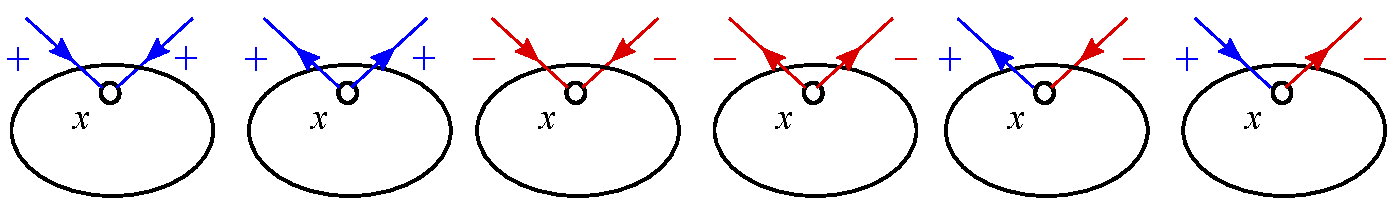
\includegraphics[width=13cm]{mismatch.pdf}} 
 %\ee
 \end{center}
%Otherwise, if the two edges connected with $x$ are of the following  forms in the following figure, then we call them  {matched}:  
%\hty{ Otherwise the two edges are  {matched} and of the following forms"}
Otherwise the two edges are {\bf matched} and of the following forms:
  \begin{center}
  %\be\label{pic match}
 \parbox[c]{0.56\linewidth}{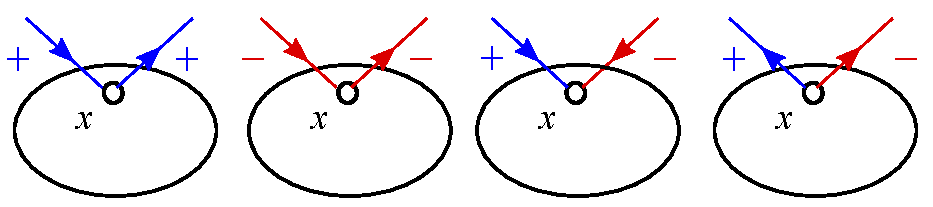
\includegraphics[width=9cm]{match.pdf}} 
 %\ee
\end{center}
Alternatively, a degree 2 atom $x$ is said to be connected with two matched edges if and only if its charge is 0, where  the charge of an atom is defined by  
$$\#\{\text{incoming $+$ and outgoing $-$ solid edges}\}- \#\{\text{outgoing $+$ and incoming $-$ solid edges}\} .$$
\end{definition}


By Definition \ref{multi-def}, we can see that if $x$ is connected with two mismatched edges, then $\cal O_{multi-e}(x) \left[\cal G\right] $ is a sum of graphs that are all of strictly higher scaling orders than $\cal G$. For example, we take  $\cal G=G_{xy}   G_{x y'}  f(G)$, i.e., $k_1=2$ and $k_2=k_3=k_4=0$ in \eqref{multi setting}. Then the first two main terms on the right-hand side of \eqref{Oe1x} are both zero. 


The following lemma describes the basic properties of multi-edge expansions. % including the expansions of mismatched edges. 
Its proof is a straightforward application of Definition \ref{multi-def}, and we postpone it to Appendix \ref{appd localpf}.
   
\begin{lemma}\label{expandmulti}
Consider a normal regular graph $\cal G$ taking the form \eqref{multi setting}, where $f (G)$ does not contain any $G$ edges or weights attached to $x$, and the atoms $y_i,$ $y'_i$, $w_i$ and $w'_i$ are all not equal to $x$. Then \smash{${\cal O}_{multi-e}^{(x)}[\cal G]$} is a canonical local expansion satisfying the following properties. 
%Then the following properties hold for $ {\cal O}_{multi-e}^{(x)}[\cal G_x]$.
\begin{itemize}
%\item[(a)] We have  $ \llbracket {\cal O}_{multi-e}^{(x)}[\cal G_x]\rrbracket  =\llbracket \cal G_x\rrbracket.$ 
%\item[(b)] In each new graph, the new atoms (if there are any) are connected to $x$ through paths of waved edges.
%\item[(c)] ${\cal O}_{multi-e}^{(x)}[\cal G_x]$ is a linear combination of normal regular graphs. \hty{ these are the same as the previous lemma. I wonder if you can just cite them? } 
\item[(a)] %If $\deg(x)\ge 4$ in $\cal G$, then every $Q$-graph in ${\cal O}_{multi-e}^{(x)}[\cal G_x]$ has scaling order $\ge \ord(\cal G_x)$, while every graph in ${\cal O}_{multi-e}^{(x)}[\cal G_x]$ without $Q$-labels  satisfies at least one of the following three properties: 
Suppose that $\deg(x)\ge 4$ in $\cal G$. Then every graph without $Q$-labels, say $\cal G_1$, in \smash{${\cal O}_{multi-e}^{(x)}[\cal G]$} either has a strictly higher scaling order than $\cal G$ or satisfies one of the following two properties:
\begin{itemize}
%\item[(d.1)] its scaling order is strictly larger than $\ord(\cal G_x)$; 
\item[(a.1)] %its scaling order is equal to 
$\ord(\cal G_1)= \ord(\cal G)$; $\cal G_1$ has one new atom with degree 2;  $\deg(x)$ in $\cal G_1$ is smaller than $\deg(x)$ in $\cal G$ by 2, and the degree of any other atom stays the same as in $\cal G$;
%in it has strictly smaller degree compared to the original graph (i.e. the above case (a)); 
\item[(a.2)] %its scaling order is equal to 
$\ord(\cal G_1)= \ord(\cal G)$; every new atom in $\cal G_1$ (if there is any) has degree 0; $\deg(x)$ in $\cal G_1$ is smaller than $\deg(x)$ in $\cal G$ by 2, and the degree of any other atom either stays the same or decreases by 2. (A new atom of degree 0 occurs when $x$ is connected with two solid edges to the same external atom $y$, e.g. $G_{xy}\overline G_{xy}$ or $G_{xy}G_{yx}$: then in the graph where $\cal O_{dot}$ assigns $\al=y$ to the new atom $\al$, this atom is connected with $y$ by a dotted edge and is not merged with $y$.)
\end{itemize}
\item[(b)] %If $\deg(x)=2$ and $x$ is connected with two mismatched solid edges, then every $Q$-graph in ${\cal O}_{multi-e}^{(x)}[\cal G_x]$ has scaling order $\ge\ord(\cal G_x)$, while  every graph in ${\cal O}_{multi-e}^{(x)}[\cal G_x]$ without $Q$-labels  has strictly higher scaling order than $\ord(\cal G_x)$.
Suppose that $\deg(x)=1$, or $x$ is connected with exactly two mismatched solid edges in $\cal G$. Then %every $Q$-graph in ${\cal O}_{multi-e}^{(x)}[\cal G]$ has scaling order $\ge \ord(\cal G)$, and 
every graph without $Q$-labels has a strictly higher scaling order than $\cal G$.
\end{itemize}
  \end{lemma}
  

 Lemma \ref{expandmulti} shows that, by applying the multi-edge expansion repeatedly, we can either make all atoms in the resulting graphs to be connected with \emph{exactly two matched solid edges}, or get $Q$-graphs and graphs of sufficiently high scaling orders. 
%The purpose of the multi-edge expansion is to make all internal atoms to have degree 0 or 2. 
%After applying the multi-edge expansions repeatedly, we get graphs where each atoms is either of degree 0 or is connected with two {\bf matched $G$ edges}. 
%Now for the atoms of degree 2 and with matched edges, we apply the following $G^2$ and  $G\overline G$ expansions. 


If an atom is connected with exactly two matched solid edges, then applying the multi-edge expansion cannot improve the graph anymore. Instead, we will apply the $G G$ expansion given by the following lemma if these two edges are of the same charge.  


  \begin{lemma} \label{T eq0}
In the setting of Theorem \ref{comp_delocal}, consider a graph $\cal G= G_{xy}   G_{y' x }  f (G)$ where $f$ is a differentiable function of $G$ and $y,y'\ne x$. Then we have that 
\be\label{G2fH}
\begin{split} 
 \cal G   &  =   m b_{xy} P_y\left[ G_{y' y} f(G)\right]  +m \sum_{\al,\beta}  b_{x\al} s_{\al\beta}P_\al\left[  (G_{\beta \beta}-m)  G_{\al y}   G_{y' \al }  f (G)\right]  \\
 & + m \sum_{\al,\beta}  b_{x\al} s_{\al\beta} P_\al\left[ (G_{\al\al}-m)   G_{\beta y}   G_{y' \beta }  f (G)\right]- m \sum_{\al,\beta} b_{x\al}    s_{\al\beta}P_\al\left[ G_{\beta y} G_{y' \al} \partial_{ h_{\beta \al}}f(G)\right]\\
  & + \sum_\al b_{x\al}  Q_\al\left[G_{\al y}   G_{y' \al}  f (G)\right]   - m^2 \sum_{\al, \beta}b_{x\al} s_{\al\beta}  Q_\al\left[ G_{\beta y}   G_{y' \beta }  f (G)\right] ,
 \end{split} 
 \ee 
% \be\label{G2fH}
% \begin{split} 
% 	\cal G   &  =   m b_{xy} P_y\left[ G_{y' y} f(G)\right]  +m \sum_{\al,\beta}  b_{x\al} s_{\al\beta}P_\al\left[  (G_{\beta \beta}-m) \cal G_\al\right]  + m \sum_{\al,\beta}  b_{x\al} s_{\al\beta} P_\al\left[ (G_{\al\al}-m)  \cal G_\beta\right]\\
% 	&- m \sum_{\al,\beta} b_{x\al}    s_{\al\beta}P_\al\left[ G_{\beta y} G_{y' \al} \partial_{ h_{\beta \al}}f(G)\right] + \sum_\al b_{x\al}  Q_\al\left(\cal G_{\al }\right)   - m^2 \sum_{\al, \beta}b_{x\al} s_{\al\beta}  Q_\al\left( \cal G_\beta\right) ,
% \end{split} 
% \ee 
where $b$ is  defined in \eqref{defn b}.
% where we denote
%$$   B:= \frac{m^2 S}{1- m^2 S}, \quad b:=  \frac{1}{1- m^2 S} = B + 1.$$
\end{lemma} 
\begin{proof}
Using \eqref{GmH} and $I_N=b - m^2 bS$, we get that  
\begin{align}
   P_x\left(  \cal G\right) & = \sum_\al \left[ b_{x\al} -m^2 (b S)_{x\al}\right] P_\al\left[G_{\al y}   G_{y' \al}f(G)\right] \nonumber\\
 %&= Q_x (G_{xy}   G_{y' x }  f (H) )-\sum_\al m^2 (b S)_{x\al} P_\al\left[G_{\al y}G_{y'\al}f(G)\right] + \sum_k b_{x\al} P_\al\left[G_{\al y}G_{y'\al}f(G)\right]  \\
   &= -\sum_\al m^2 (b S)_{x\al}  P_\al\left[G_{\al y}   G_{y' \al}f(G)\right] + \sum_\al  b_{x\al} P_\al\left[ \left(m\delta_{\al y}-m^2G_{\al y} - m (HG)_{\al y}\right) G_{y' \al} f(G)\right] .\label{dervG2}
  \end{align}
 Applying Gaussian integration by parts to the $ HG $ term, we get that
\begin{align*}
   &P_\al\Big[  -m \sum_\beta h_{\al\beta}G_{\beta y} G_{y' \al} f(G)\Big] \\
   =& P_\al\Big[ m \sum_\beta  s_{\al\beta}G_{\beta\beta} G_{\al y}   G_{y' \al}f(G) + m \sum_\beta s_{\al\beta} G_{\al\al}  G_{\beta y}   G_{y' \beta}f(G) - m \sum_\beta s_{\al\beta}G_{\beta y} G_{y' \al} \partial_{ h_{ \beta \al}}f(G)\Big].
\end{align*}
Plugging it into \eqref{dervG2},  using $1=P_x+Q_x$, $\delta_{x\al}+m^2 (b S)_{x\al}=b_{x\al}$ and 
\begin{align*}
& \, m \sum_{\al, \beta}b_{x\al} s_{\al\beta}  P_\al\left[G_{\al\al}  G_{\beta y}   G_{y' \beta}f(G)\right] -\sum_\al m^2 (b S)_{x\al}  P_\al\left[G_{\al y}   G_{y' \al}f(G) \right] \\
=&\,  m \sum_{\al, \beta}b_{x\al} s_{\al\beta}  P_\al\left[  (G_{\al\al}-m)  G_{\beta y}   G_{y' \beta}f(G)\right] + \sum_\al m^2 (b S)_{x\al}  Q_\al\left[G_{\al y}   G_{y' \al}f(G)\right] \\
&\,   - m^2 \sum_{\al, \beta}b_{x\al} s_{\al\beta}  Q_\al\left[G_{\beta y}   G_{y' \beta}f(G)\right] ,
\end{align*}
 we  obtain equation \eqref{G2fH}. 
  \end{proof}


%There is an alternative way to derive \eqref{dervG2}. \hty{we should talk about this}  Applying \eqref{Oe1x} with $k_1=k_3=1$ and $k_2=k_4=0$, we have that for $\cal G_x= G_{xy}   G_{y' x }  f (G)$,
%\begin{align*} 
%   \cal G_x - m^2  \sum_\al s_{x\al }\cal G_\al & =   m  (G_{xx}-m) \sum_\al s_{x\al }\cal G_\al +  m   \sum_\al s_{x\al }\left(G_{\al \al}-m\right) \cal G_x  \nonumber \\
%& - m    \sum_\al s_{x\al }  G_{\al y} G_{y' x} \partial_{ h_{\al x}}f (G) +\cal Q_{multi-e}.
%%& + Q_x \left( \cal G_x\right)   -   m Q_x \left[ G_{xx}  \sum_\al s_{x\al }\cal G_\al\right] -  m Q_x \left[  \sum_\al s_{x\al }\left(G_{\al \al}-m\right) \cal G_x\right]  +m Q_x \left[  \sum_\al s_{x\al } G_{\al y}G_{y' x} \partial_{h_{\al x}}f(G)  \right].
%\end{align*}
%Multiplying both sides by the matrix $b$ in \eqref{defn b}, we  obtain \eqref{G2fH}. However, there is a caveat that $\cal G_y$ and $\cal G_{y'}$ actually satisfy a different expansion, which makes the derivation a little more complicated. %In the above proof, we used a more direct way to prove \eqref{G2fH}.  


Using \eqref{G2fH}, $b =1 + S^+ $ and $P_\al=1-Q_\al$, we can define the following $G G$ expansion operator. 
   \begin{definition}[$G G$ expansion operator] \label{GG-def}
  Given a normal regular graph $\cal G$, suppose an atom $x$ is connected with exactly two matched $G$ edges of the same charge. Suppose $\cal G$ takes the form $\cal G=G_{xy}   G_{y' x } f(G)$ with $y,y' \ne x$. Then we define
\begin{align}
  \wh{\cal O}_{GG}^{(x)} [\cal G] & := %m\delta_{xy} G_{y' y} f(G) + 
m S^{+}_{xy} G_{y' y} f(G)  + m \sum_\al  s_{x\al} (G_{\al \al}-m) \cal G + m \sum_{\al,\beta}  S^{+}_{x\al}  s_{\al\beta} (G_{\beta \beta}-m) G_{\al y}   G_{y'\al} f(G) \nonumber \\
    &  + m(G_{xx }-m)   \sum_\al s_{x\al}G_{\al y}   G_{y'\al} f(G) + m \sum_{\al,\beta}  S^+_{x\al} s_{\al\beta}  (G_{\al\al }-m) G_{\beta y}   G_{y'\beta} f(G)  \nonumber\\
    & - m \sum_{ \al}  s_{x\al}G_{\al y} G_{y' x} \partial_{ h_{\al x}}f(G) - m \sum_{\al,\beta} S^{+}_{x\al} s_{\al\beta}G_{\beta y} G_{y' \al} \partial_{ h_{\beta \al}}f(G) + \cal Q_{GG} .\label{Oe2x}
    \end{align}
On the right-hand side of \eqref{Oe2x}, the first term is the main term which is either of the same scaling order as $\cal G$ if $y=y'$ or has a strictly higher scaling order if $y\ne y'$; the second to fifth terms contain one more light weight and hence are of strictly higher scaling orders than $\cal G$; the sixth and seventh terms contain at least one more off-diagonal $G$ edge and hence are of strictly higher scaling orders than $\cal G$. The last term $\cal Q_{GG} $ is a sum of $Q$-graphs defined by
    \begin{align}
  \cal Q_{GG}&:=  Q_x \left(\cal G\right)+  \sum_\al Q_\al\Big[ S^+_{x\al}  G_{\al y}   G_{y'\al} f(G) \Big]  - m Q_y\Big[S^{+}_{xy}  G_{y' y} f(G)\Big] - m Q_x\Big[\sum_\al  s_{x\al} (G_{\al\al}-m) \cal G\Big]  \nonumber\\
   &- m \sum_\al Q_\al\Big[\sum_{ \beta}  S^{+}_{x\al}  s_{\al\beta} (G_{\beta \beta}-m)G_{\al y}   G_{y'\al} f(G)\Big] - mQ_x\Big[ G_{xx }  \sum_\al s_{x\al} G_{\al y}   G_{y'\al} f(G)\Big] \nonumber\\
&- m\sum_\al Q_\al\Big[ \sum_{ \beta}  S^{+}_{x\al}  s_{\al\beta} G_{\al\al }  G_{\beta y}   G_{y'\beta} f(G)\Big]  + m Q_x\Big[\sum_{ \al}  s_{x\al} G_{\al y} G_{y' x} \partial_{ h_{ \al x}}f(G)\Big] \\
& + m\sum_\al Q_\al\Big[ \sum_{\beta} S^{+}_{x\al} s_{\al\beta}G_{\beta y} G_{y' \al} \partial_{h_{\beta \al}}f (G)\Big] .\nonumber 
 \end{align}
On the other hand, if $\cal G=\overline G_{xy}  \overline G_{y' x }  f(G)$, then we define 
$$\wh{\cal O}_{GG}^{(x)}\left[\cal G\right]:=\overline{ \wh{\cal O}_{GG}^{(x)}\left[G_{xy}   G_{y' x }  \overline{f(G)}\right] },$$
where the right-hand side can be defined using \eqref{Oe2x}. If $y$ is an external atom and $y'$ is an internal atom, then we instead use the expansion obtained by applying \eqref{Oe2x} to $H^\top$ (which satisfies the same assumptions as $H$ and whose resolvent is $G^\top$) with $y$ and $y'$ interchanged, and then transposing all $G$ entries back. Its leading term is $m S^{+}_{xy'} G_{y' y} f(G)$ (resp.~$\overline m S^{-}_{xy'} \overline G_{y' y} f(G)$ if $\cal G=\overline G_{xy}  \overline G_{y' x }  f(G)$), whose waved edge joins $x$ to the internal atom $y'$, and the corresponding $Q$-term $-m Q_{y'}[S^{+}_{xy'} G_{y' y} f(G)]$ has its $Q$-label at $y'$. We still denote this expansion by $\wh{\cal O}_{GG}^{(x)}[\cal G]$. Finally, we define
$${\cal O}_{GG}^{(x)}[ \cal G]:= \cal O_{dot} \circ  \wh{\cal O}_{GG}^{(x)}   [\cal G]. $$  
%If $x$ is an internal atom in a graph $\cal G=\sum_x \cal G_x$, then we naturally define the $GG$ expansions of $\cal G$ on atom $x$ as %(recall the linearity \eqref{linear graphO})
%$\sum_x {\cal O}^{(x)}_{GG} [\cal G_x ] .$
\end{definition}




 We describe the basic properties of the $GG$ expansions in the following lemma. Its proof is straightforward by using Definition \ref{GG-def}, and we postpone it to Appendix \ref{appd localpf}.
  \begin{lemma}\label{expandG2}
 Given a normal regular graph $\cal G = G_{xy}   G_{y' x } f(G)$, where $f(G)$ contains no weights or solid edges attached to $x$  and $y,y'\ne x$. %Then the following properties hold for ${\cal O}_{GG}^{(x)}[ \cal G_x]$.
 %Then \smash{${\cal O}_{multi-e}^{(x)}[\cal G]$} is a canonical local expansion and satisfies % the same properties (a)--(c) as in Lemma \ref{expandlabel} and 
 %the following properties. 
Then \smash{${\cal O}_{GG}^{(x)}[ \cal G]$} is a canonical local expansion. %satisfies the same properties (a)--(c) of  Lemma \ref{expandlabel} and  every $Q$-graph in \smash{${\cal O}_{GG}^{(x)}[ \cal G_x]$} has scaling order $\ge \ord(\cal G_x)$ and 
Moreover, every graph without $Q$-labels, say $\cal G_1$, in \smash{${\cal O}_{GG}^{(x)}[ \cal G]$} satisfies one of the following properties. 
\begin{itemize}
\item[(a)] If $y\not = y'$, then $\cal G_1$ has a strictly higher scaling order than $\cal G$.


\item[(b)] If $y = y'$, then either $\cal G_1$ has a strictly higher scaling order than $\cal G$, or $\cal G_1$ is obtained by replacing $G_{xy} G_{yx}$ in $\cal G$ with $m S^+_{xy}G_{yy}$.
\end{itemize}
%\eqref{strict_high} or the following property corresponding to the first term in \eqref{Oe2x}:
% 
% \begin{itemize}
%%\item[(a)] We have $ \llbracket {\cal O}_{GG}^{(x)}[\cal G_x]\rrbracket  =\llbracket \cal G_x\rrbracket.$ 
%%\item[(b)] In each new graph, the new atoms (if there are any) are connected to $x$ through paths of waved edges.
%%\item[(c)] ${\cal O}_{GG}^{(x)}[\cal G_x]$ is a linear combination of normal regular graphs. \hty{ again, this is a repetition} 
%%\item[(d)] Every $Q$-graph in ${\cal O}_{GG}^{(x)}[\cal G_x]$ has scaling order $\ge\ord(\cal G_x)$. 
%
%\item[(a)] $\cal G_1$ is obtained by replacing $G_{xy} G_{y'x}$ in $\cal G_x$ with $m S^+_{xy}G_{y'y}$. 
%%Each new graph without any $Q$-label has scaling order  strictly higher than $\ord(\cal G_x)$ unless $y=y'$ and \hty{it's not clear what the following means} the graph is obtained by replacing $G_{xy}   G_{yx }$ in $\cal G_x$ with $m S^+_{xy}G_{yy}$. 
%%while every graph in ${\cal O}_{GG}^{(x)}[\cal G_x]$ without $Q$-labels, say $\cal G_1$, satisfies at least one of the following properties. 
%%\begin{enumerate}
%%\item $\ord(\cal G_1)\ge \ord(\cal G_x) +1$.
%%\item $\ord(\cal G_1)= \ord(\cal G_x)$, and $\cal G_1$ is obtained by replacing a pair of positive edges (or a pair of negative edges) between $x$ and another atom, say $y$, with $m S^{+}_{xy} G_{y y}$ (or $m S^{-}_{xy} \overline G_{y y}$). In particular, we have $\deg(x)=0$ and the degree of $y$ is decreased by 2.
%%\end{enumerate}
%\end{itemize}
%\hty{
%say $\cal G_1$, either satisfies \eqref{strict_high} or 
%\be
%\text{ $\cal G_1$ is obtained by replacing $G_{xy} G_{y'x}$ in $\cal G_x$ with $m S^+_{xy}G_{y'y}$.}
%\ee
%}
Similar statements hold if $\cal G = \overline G_{xy}   \overline  G_{y' x } f(G)$. 
\end{lemma}

%The last property (e) 
%\cob
%For the graph $\cal G_1$ in (a), it either satisfies \eqref{strict_high} when $y\ne y'$, or $\ord(\cal G_1)= \ord(\cal G_x)$ when $y= y'$. \nc 


Lemma \ref{expandG2} shows that, by applying the $GG$ expansion repeatedly, we can either get rid of atoms %\hty{ get rid of atoms? } 
that are connected with a pair of edges of the same charge, or obtain $Q$-graphs and graphs of sufficiently high scaling orders. 
%The purpose of the $GG$ expansion is to remove all the non-neutral atoms (i.e. atoms that are connected with a pair of edges of the same charge). 

%\iffalse
%If all internal atoms of a graph are either of degree $0$ or connected with a pair of matched solid edges of opposite charges,  then none of the previous expansions can be applied to improve this graph.  \hty{ why not say that "we can only apply the $G \bar G$ expansion which we will explain later on. The reason is that it is not clear what "improve means. Also, $G \bar G$ expansion is a special case of previous expansion. The other choice is just to define standard neutral quickly and avoid this para } 
%At this stage, we have to apply the $\Theta$-expansion in Lemma \ref{expandtheta} (or more generally 
%a lower order $T$-expansion if we do it inductively)  to this graph. To prepare for this expansion, we define the following notion. 
%
%
%\hty{ maybe we can remove the following para  which is too long} 
%Recalling that the $\Theta$-expansion is essentially a second order $T$-expansion, a more general expansion is to replace a pair of solid edges with a lower order $T$-expansion. However, for both the $\Theta$-expansion and the lower order $T$-expansions, they can only be applied to the $T$-variables. Inspired by this discussion, 
%\fi

Now we define the following concept of \emph{standard neutral atoms}. Roughly speaking, the edges connected with a standard neutral atom almost form a $T$-variable (but not an exact $T$-variable because of the $\times$-dotted edges; see Section \ref{subsec global} for more details).


 \begin{definition}[{Standard neutral atoms}]\label{def SNA}
An atom is said to be \emph{standard neutral} if it is only connected with three edges besides the $\times$-dotted edges: two {matched} $G$ edges of {opposite charges} and one waved $S$ edge. 
 \end{definition}
 
Given a graph with a non-standard neutral atom $x$ (for example, the atom $x$ in graph (f) of \eqref{Aho3} below) that is connected with two matched $G$ edges of opposite charges, we can apply the following $G\overline G$ expansion. The $G\overline G$ expansion \eqref{Oe3x} is a special case of the multi-edge expansion in Definition \ref{multi-def} with $k_1=k_2=1$, $k_3=k_4=0$ or $k_1=k_2=0$, $k_3=k_4=1$.

\begin{definition} [$G\overline G$ expansion operator]\label{GGbar-def} 
Given a normal regular graph $\cal G$, suppose the atom $x$ is connected with exactly two matched $G$ edges of opposite charges,  and $\cal G$ takes the form $\cal G= G_{xy}  \overline G_{xy'} f(G)$ with $y,y' \ne x$.  % \hty{ this is confusing. I thought that we can't improve on it already? it seems some cases you can still improve on it? }
%However, $x$ may {\bf not} be connected with {\bf only one $s$ edge}. 
Then we define  
\begin{align}
 \wh{\cal O}_{G\overline G}^{(x)}[\cal G] &:=   |m|^2  \sum_\al s_{x\al }G_{\al y} \overline G_{\al y'} f(G) + m \sum_\al s_{x\al }\left(G_{\al \al} -m \right) \cal G \nonumber  \\
&  +  m (\overline G_{xx} - \overline m)   \sum_\al s_{x\al }G_{\al y} \overline G_{\al y'} f(G)  - m  \sum_\al s_{x\al }G_{\al y}  \overline G_{xy'} \partial_{ h_{\al x}} f(G) + \cal Q_{G\overline G}, \label{Oe3x}
 \end{align}
  where on the right-hand side, the first term is of the same scaling order as $\cal G$, and the new atom $\al$ is standard neutral; the second and third terms  contain one more light weight and hence are of strictly higher scaling orders than $\cal G$; the fourth term  contains at least one more off-diagonal $G$ edge and hence is of strictly higher scaling order than $\cal G$. The last term $\cal Q_{G\overline G} $ is a sum of $Q$-graphs defined by
 \begin{align*}
 \cal Q_{G\overline G}&:= Q_x \left(\cal G\right) -  m Q_x\Big[ \sum_\al s_{x\al }\overline G_{xx}G_{\al y} \overline G_{\al y'} f(G) \Big] - m Q_x\Big[\sum_\al s_{x\al }\left(G_{\al \al} -m \right) \cal G\Big] \\
 & + mQ_x\Big[  \sum_\al s_{x\al }G_{\al y}  \overline G_{xy'} \partial_{ h_{\al x}} f(G) \Big].
\end{align*}
On the other hand, if $\cal G= G_{yx}  \overline G_{y'x} f(G)$, then we define $\cal O_{G\overline G}(x)[ \cal G] $ by taking $k_1=k_2=0$ and $k_3=k_4=1$ in Definition \ref{multi-def}, and we omit the explicit expression for simplicity.  Finally, we define
$${\cal O}_{G\overline G}^{(x)}[ \cal G]:= \cal O_{dot} \circ  \wh{\cal O}_{G\overline G}^{(x)}   [\cal G]. $$  
%If $x$ is an internal atom in a graph $\cal G=\sum_x \cal G_x$, then we define the $G\overline G$ expansions of $\cal G$ on atom $x$ as %(recall the linearity \eqref{linear graphO})
%If $x$ is an internal atom, then we define $ {\cal O}^{(2)}_{weight}(x)[\cal G]$ using \eqref{linear graphO} as 
%\be\label{eq defOdot0}
%$\sum_x {\cal O}^{(x)}_{G\overline G} [\cal G_x ] .$
%\iffalse
%as %if the graph is of the form $\cal G=\sum_{x,y,y'} G_{yx}  \overline G_{y'x} f_x(G,y,y')$, then we have 
%\begin{align} 
%& \wh{\cal O}_{G\overline G}(x)[ G_{yx}  \overline G_{y'x} f_x(G) ] =   |m|^2  \sum_\al s_{x\al }G_{y\al} \overline G_{y' \al } f_x(G)   \nonumber\\
%&+ \sum_\al s_{x\al }\left(G_{\al \al} -m \right) G_{yx}  \overline G_{y'x} f_x(G)  +  m (\overline G_{xx} - \overline m)    \sum_\al s_{x\al }G_{y\al} \overline G_{y'\al}  f_x(G)   \nonumber \\
%& - m  \sum_\al s_{x\al }G_{y\al}  \overline G_{y'x} \partial_{\overline h_{\al x}} f_x(G) + \cal Q_{G\overline G}, \nonumber %\label{Oe3x2}
% \end{align}
%  where 
% \begin{align*}
% \cal Q_{G\overline G}&:= Q_x [ G_{yx}  \overline G_{y'x} f_x(G) ] -  m Q_x\left[ \sum_\al s_{x\al }\overline G_{xx}G_{y\al } \overline G_{ y'\al} f_x(G) \right] - m Q_x\left[\sum_\al s_{x\al }\left(G_{\al \al} -m \right) G_{yx}  \overline G_{y'x} f_x(G)\right] \nonumber\\
%&  + m Q_x\left[ \sum_\al s_{x\al }G_{y\al}  \overline G_{y'x} \partial_{\overline h_{\al x}} f_x(G) \right].
%\end{align*}
%Finally, $\widehat{\cal O}_{G\overline G}(x) \left[\cal G\right]$ is defined by using \eqref{linear graphO}, and we define
%$${\cal O}_{G\overline G}(x)[ \cal G]:= \cal O_{dot} \circ  \wh{\cal O}_{G\overline G}(x)   [\cal G]. $$ 
%\fi 
\end{definition}

The purpose of the $G\overline G$ expansion is to turn the non-standard neutral atom $x$ into a new standard neutral atom $\al$ in the first term. The following lemma describes the basic properties of the $G\overline G$ expansion. Its proof is straightforward by using Definition \ref{GGbar-def}, and we postpone it to Appendix \ref{appd localpf}.  
  \begin{lemma}\label{expandGGbar}
  Given a normal regular graph $\cal G= G_{xy}  \overline G_{xy'} f(G)$, where $f(G)$ contains no weights or solid edges attached to $x$  and $y,y'\ne x$. Then \smash{${\cal O}_{G\overline G}^{(x)}[ \cal G]$} is a canonical local expansion. 
  %satisfies the same properties (a)--(c) as in Lemma \ref{expandlabel}. Moreover, every $Q$-graph in ${\cal O}_{G\overline G}^{(x)}[ \cal G_x]$ has scaling order $\ge \ord(\cal G_x)$, and 
  Moreover, every graph without $Q$-labels, say $\cal G_1$, in \smash{${\cal O}_{G\overline G}^{(x)}[ \cal G]$} either has a strictly higher scaling order than $\cal G$, or satisfies one of the following properties:
  %Then the following properties hold for ${\cal O}_{G\overline G}^{(x)}[ \cal G_x]$.
   % Given a normal regular graph $\cal G$, suppose it has a non-standard neutral internal atom $x$ connected with two matched solid edges of opposite charges. 
%  \begin{itemize}
% \item[(a)] We have $ \llbracket {\cal O}_{G\overline G}^{(x)}[\cal G_x]\rrbracket  =\llbracket \cal G_x\rrbracket.$  
% \item[(b)] In each new graph, the new atoms (if there are any) are connected to $x$ through paths of waved edges.
%\item[(c)] ${\cal O}_{G\overline G}^{(x)}[\cal G_x]$ is a linear combination of normal regular graphs. 
% 
% \item[(d)] Every $Q$-graph in ${\cal O}_{G\overline G}^{(x)}[\cal G_x]$ has scaling order $\ge\ord(\cal G_x)$, while any graph in ${\cal O}_{G\overline G}^{(x)}[\cal G]$ without $Q$-labels, say $\cal G_1$, satisfies at least one of the following properties. 
\begin{enumerate}
%\item[(d.1)] $\ord(\cal G_1)\ge \ord(\cal G) +1$.
\item[(a)] $\ord(\cal G_1)= \ord(\cal G)$, $\deg(x)=0$ in $\cal G_1$, and $\cal G_1$ contains one more standard neutral atom;
\item[(b)] $\ord(\cal G_1)= \ord(\cal G)$, and $\cal G_1$ is obtained by replacing $G_{xy}  \overline G_{xy}$ with $|m|^2 s_{xy} |G_{y y}|^2$ in the $y=y'$ case. %In particular, we have $\deg(x)=0$ and the degree of $y$ is decreased by 2.
\end{enumerate}
%\end{itemize}
Similar statements hold if $\cal G = G_{y x}   \overline  G_{y' x } f(G)$.

%\hty{ All these properties are repeated several times. It's best to give names to them and then just cite them} 
  \end{lemma}
 

Lemma \ref{expandGGbar} shows that by applying the $G\overline G$ expansions repeatedly, we can get either new graphs containing only standard neutral atoms and degree 0 atoms, or $Q$-graphs and graphs of sufficiently high scaling orders.
In Lemmas \ref{expandlabel}, \ref{expandmulti} and \ref{expandGGbar}, the degrees and weights in the alternatives with the same scaling order, and the condition $y=y'$ in Lemma \ref{expandGGbar}, are taken per block of atoms connected by dotted edges (such blocks may contain external atoms); the claims on the scaling orders are unchanged.
%can either remove all the non-standard neutral atoms, or get $Q$-graphs and graphs of sufficiently high scaling orders. 
%Note that the three edges connected with a standard neutral atom form a generalized $T$ variable (actually, it is not exactly a $T$-variables because of the $\times$-dotted edges associated with the two solid edges, but the difference can be handled rather easily). Then we can apply a lower order $T$-expansion \eqref{mlevelTgdef} to these three edges. 

%The operation of replacing a $T$-variable with a lower order $T$-expansion. 
%This is called a \emph{global expansion} instead, which will be discussed in Section \ref{sec global}.


\subsection{Local expansion strategy} 

%By applying the basic weight and edge expansions repeatedly, 

%*******************
%We shall call the weight and edge expansions in Sections \ref{sec localexp} and \ref{sec localexp edge} as \emph{local expansions}. \hty{ local expansion nama was used earlier. One need to explain local expansion earlier.} To explain this name, we introduce the following concept of molecules. 
%
%%As discussed in Section \ref{sec strategy}, each of our graph has a two-level structure, that is, a local structure on the scale $W$, and a global structure on the scale $L$. To organize the two-level structure, we introduce the following concept of molecules. 
%
%%We first introduce the concept of molecules for the graphs defined in Section \ref{unisec}.
%
%\begin{definition}[Molecules]\label{def_poly}
% We partition the set of all atoms into a union of disjoint sets $\{\text{all atoms}\}=\cup_j \cal M_j$, where each $\cal M_j$ is called a molecule. Two internal atoms belong to the same molecule if and only if they are connected with a path of neutral/plus/minus {\bf waved edges} and {\bf dotted edges} (note there may be dotted edges \cor  between internal atoms \nc if the graph is not regular). 
%%For the atoms in the same molecules, we always combine them if they are the same (i.e. if they are connected by a dotted line). %Moreover, we assign a dash-dotted line partition of them, that is each two atoms in the same molecule are connected through a cross dah-dotted edge. We do not assign dah-dotted line partitions to all the graph, that is, atoms in different molecules can be the same (except in some middle steps of the expansions, in which case we will mention it explicitly). 
%Each external atom will \cor by definition \nc  be  called an external molecule (such as $\otimes$, $\oplus$ and $\ominus$ molecules).  An edge is said to be inside a molecule if \cor its \nc  ending atoms  belong to this molecule.
%\end{definition}
%%\begin{remark}
%By \eqref{subpoly} and \eqref{S+xy}, if two atoms $x$ and $y$ are in the same molecule, then we  have essentially $|x-y|\le W^{1+\tau}$ up to a negligible error $\OO(W^{-D})$. % \hty{probably remove the rest of this sentence. It seems to be more confusing to have them} in the sense of graph values in all the expressions. 
%Given an atomic graph, we will call the subgraph inside a molecule (i.e. the subgraph induced on the atoms inside this molecule) the  {\it local structure} \cor of the molecule.  A \emph{molecular graph} (cf. Definition \ref{def moleg} below) is the  quotient graph with each molecule regarded as a vertex. \nc  
%We call the structure of the molecular graph the {\it global structure}.  \hty{ The {\it global structure} of a graph is by definition the molecular graph}
%Note that the local structures can only vary on scales of order $\OO (W^{1+\tau})$, while the global structure varies on scales \cor up to  $L$. \nc The \emph{two-level structure} of an atomic graph---a global structure plus several local structures---has been explored in \cite{PartIII} already. 
%
%%As discussed in Section \ref{sec strategy}, each of our graph has a two-level structure, that is, a local structure on the scale $W$, and a global structure on the scale $L$. To organize the two-level structure, ..........
%******************



%
%The goal of local expansions is to expand a regular graph into the following \emph{locally standard graphs}, which (locally) consist of \cor $T$-variables, $Q$-graphs \nc and higher order graphs. For any locally standard graph, we cannot apply local expansions to improve it %\hty{ remove essential} 
%in any way; the global expansions have to come into play, which will be discussed in Section \ref{subsec global}.
% 
%Recall \eqref{degree}, for any molecule $\cal M_i$, $\deg (\cal M_i)$ denotes the number of solid edges that connect the atoms in $\cal M_i$ to the atoms outside the molecule. 
 
We define the concept of \emph{locally standard graphs}.

 \begin{definition} [Locally standard graphs] \label{deflvl1}%   \cob (need details) \nc 
A graph $\cal G$ is  \emph{locally standard}  if 
 % The goal of the Level 1 expansions is to expand the input graphs into {\bf level 1 standard graphs}. A {\bf level 1 standard graph} is graph such that:
\begin{itemize}
\item[(i)] it is a normal regular graph without $P/Q$ labels; % (recall Definition \ref{defnlvl0});  

%\item[(ii)] all the edges in the graph have no independent sets;

%\item[(ii)] any two atoms in the same molecule are different, and there is a $\times$-dotted edge between them;

\item[(ii)] it has no weights or light weights;

\item[(iii)] the degree of any internal atom is $0$ or $2$; % (recall \eqref{degree}); %that is connected with solid $G$ edges must have degree 2 (at this step, the two edges can be of the same or different charges), and is connected with one waved $S$ edge;

\item[(iv)] all degree 2 internal atoms are \emph{standard neutral atoms}. % (recall Definition \ref{def SNA}).%, that is, it is connected to exactly three edges---two {\bf matched} $G$ edges of {\bf opposite charges} and one waved $S$ edge---besides the $\times$-dotted edges. %if a internal atom is connected with two $G$ edges, then these two edges must be of opposite charges; 

%\item[(v)] it satisfies the {\bf off-$G$-property}, that is, every $G$ edge is associated with a $\times$-dotted line; %, that is, for any atoms $\al,\beta$ in the graph, there is a $\times$-dotted edge between them {\bf if} there is at least one $G$ edge between them (\cor every $G$ is associated with $\times$-dotted line\nc); 

%\item[(v)]  it satisfied the {\bf reverse off-$G$-property}, that is, for any pair of atoms $\al,\beta$ in the graph, there is a $\times$-dotted edge between them {\bf only if} there is at least one $G$ edge between them (in other words, if there is no $G$ edge between these two atoms, then they are not connected by a $\times$-dotted edge). 

%\item[(vii)] %for any neutral atom with degree 2, it is only connected to a neutral waved edge (i.e. $s$ edge) except for the two $G$ edges (\cor 
%any neutral atom with degree 2 is connected to three edges, two $G$ edges of opposite charges and one $s$ edge.
\end{itemize}
 %We shall call degree 2 neutral atoms satisfying (vii) ``standard neutral atoms".
 \end{definition}
% \begin{remark}
%%Note that property (iv) has already been contained in Definition \ref{defnlvl0} of normal regular graphs, although we state it here for emphasis. 
%For property (v) to hold, if atoms $\al$ and $\beta$ are not connected by $G$ edges, but there is a $\times$-dotted line between them, then we use $\cal O_{rDot}$ in \eqref{ordot} to remove this $\times$-dotted line. The main purpose of this property is to ensure that our deterministic graphs contain no $\times$-dotted lines in the end.
%%$\Sdelta^{(n)}$ in \eqref{mlevelTgdef} and $\wtSdeltan$ in \eqref{mlevelTgdef incomp} will contain no $\times$-dotted lines finally. 
%\end{remark}


Applying local expansions in Definitions \ref{dot-def}, \ref{Ow-def}, \ref{multi-def}, \ref{GG-def} and \ref{GGbar-def} repeatedly, we can  expand any regular graph into a linear combination of locally standard, recollision, higher order and $Q$ graphs. The expansions will be performed according to the flow chart in Figure \ref{Fig chart1}. More precisely, given a regular graph $\cal G$, we first apply $\cal O_{dot}$ to expand it into a sum of %\hty{ we can from now on remove a linear combination of} 
normal regular graphs, then apply the weight expansion to remove the weights, and then apply the multi-edge, $GG$  and $G\overline G$ expansions one by one to remove all  atoms that are not standard neutral.  After an expansion, we may need to perform  earlier expansions to the resulting graphs. For example, after a multi-edge expansion, we may get graphs that contain weights. Then before performing another multi-edge expansion, we first need to perform weight expansions to these graphs. This explains why we have loops in Figure \ref{Fig chart1}.


%given a graph $\cal G$, we expand it by applying a proper graph operator to $\cal G$. 
%%into a linear combination of some new graphs; then 
%Then for each new graph from the expansion, we expand it further by applying another graph operator, and so on. 
%%into a linear combination of some new graphs, and so on. 
%We emphasize that each step of expansion is performed on a new graph, and the old graphs will not be used anymore. 

To describe precisely the local expansion process in  Figure \ref{Fig chart1}, we  define the following  stopping rules.  
%We consider the graphs in the expansions of the $T_{\fa,\fb_1\fb_2}$ variable, where we recall the notation in \eqref{rep_abc}. \hty{ I suppose that you jsut want to describe the expansion of $T_{\fa,\fb_1\fb_2}$}  
Given a cut-off order $n$, we stop the expansion of a graph if it is a normal regular graph %satisfies the off-$G$-property 
and satisfies at least one of the following properties:
\begin{itemize}
\item[(S1)] it is locally standard;

\item[(S2)] it is a $\oplus$/$\ominus$-recollision graph;

\item[(S3)] its scaling order is at least $n+1$; 

\item[(S4)] it is a $Q$-graph.
\end{itemize}

\begin{figure}
\color{black}
\tikzstyle{startstop} = [rectangle,rounded corners, minimum width=1cm,minimum height=0.5cm,text centered, draw=black]
\tikzstyle{startstop3} = [rectangle,rounded corners, minimum width=3cm, text width=8em, minimum height=0.5cm,text badly centered, draw=black]
\tikzstyle{block} = [rectangle, draw=black, %fill=blue!20, 
    text width=6em, text centered, rounded corners, minimum height=1.5em]
\tikzstyle{line} = [draw=black, -latex']
\tikzstyle{line0} = [draw=black]
\tikzstyle{decision} = [diamond, draw=black, %fill=blue!20, 
    text width=4.5em, text badly centered, node distance=2cm, 
    inner sep=0pt]

\tikzstyle{cloud} = [draw=black, ellipse, %fill=red!20, 
node distance=2.5cm,
    minimum height=2em]
\tikzstyle{null} = [draw=none,fill=none,right]

\begin{center}  
\begin{tikzpicture}[node distance = 1.1cm, auto]

    % Place nodes
    \node [startstop] (start) {Start: input graphs};
    \node [block, below of= start] (op1) {$\cal O_{dot}$};
    %\node [block, below of=op1] (op1_5) {$\cal O_{rDot}$}; 
    \node [block, below of=op1] (op2) {${\cal O}_{weight}$};
    %\node [decision, below of=op2, node distance=1.5cm] (decide2) {Check}; 
    \node [block, below of=op2] (op3) {$\cal O_{multi-e}$};
    %\node [decision, below of=op3, node distance=1.5cm] (decide3) {Check }; 
    \node [block, below of=op3] (op4) {$\cal O_{GG} $};
    %\node [decision, below of=op4, , node distance=1.5cm] (decide4) {Check }; 
    \node [block, below of=op4] (op5) {$\cal O_{G\overline G}$};
    \node [startstop3, below of=op5] (stop_LS) {Locally standard};
    %\node [null, below of=op5] (stopE) {}; 
    %\node [block, below of= op5] (op6) {$\cal O_{G\overline G}$};
    %\node [decision, below of=op6,  node distance=1.5cm] (decide6) {Check };
    %\node [block, below of= op6] (op7) {Operation G};
    %\node [block, below of=op5] (evaluate) {evaluate candidate models};
    %\node [cloud, left of=op2, node distance=4cm] (update) {Restart};
    %\node [block, below of=decide6, node distance=2cm] (op7) {Operation G};
    %\node [startstop, right of=op7, node distance=4cm] (stop) {Output $\cal A^{(1)}_x(\Gamma_1)$};
    \node [decision, right of=op3, node distance=4cm] (decide_stop) {Check (S2)-(S4)};    
    
    \node [startstop3, right of=decide_stop, node distance=3.5cm] (stop2) {Recollision; higher order; $Q$-graph.};
    
    %\node [cloud, left of=start] (Input) {Input $M$};
    %\node [cloud, right of=op1] (system) {system};
    % Draw edges
    \path [line] (start) -- (op1);
    \path [line] (op1) -- (op2);
    %\path [line] (op1_5) -- (op2);
    %\path [line] (op2)--(decide2);
    \path [line] (op2) --node [midway] {No} (op3);
    %\path [line] (op3) -- (decide3);
    \path [line] (op3) --node [midway] {No} (op4);
    %\path [line] (op4) -- (decide4);
    \path [line] (op4) --node [midway] {No} (op5);
    %\path [line] (op5) -- (stopE);
    %\node [null, left of=decide1, node distance=4.12cm] (null1) {};
%    \node [null, left of=op2, node distance=4.12cm] (null2) {};
%    \node [null, right of=op2, node distance=4.12cm] (null22) {};
%    \node [null, left of=op3, node distance=4.12cm] (null3) {};
%    \node [null, right of=op3, node distance=4.12cm] (null33) {};
%    \node [null, left of=op4, node distance=4.12cm] (null4) {};
%    \node [null, right of=op4, node distance=4.12cm] (null44) {};
    %\path [line] (decide1) -- node [midway] {yes} (null1);
    %\path [line] (op1) -| node [near start] {Stop} (stop2);
    
    \path [line] (op2) -- node [midway] {Yes} (decide_stop);
    \path [line] (op3) -- node [midway] {Yes} (decide_stop);
    \path [line] (op4) -- node [midway] {Yes} (decide_stop);
    \path [line] (op5) -| node [near start] {Yes} (decide_stop);
    \path [line] (decide_stop) -- node [midway] {Yes} (stop2);
    \path [line] (decide_stop) |- node [near end] {No} (op1);
    
    %\path [line] (op2) -- node [midway] {Stop} (null22);
    %\path [line] (op2) -- node [midway] {yes} (update);
%    \path [line] (decide2) -- node [midway] {Stop} (null22);
%    \path [line] (op3) -- node [midway] {yes} (null3);
%    \path [line] (op3) -- node [midway] {Stop} (null33);
%    \path [line] (op4) -- node [midway] {Stop} (null44);
%    \path [line] (op4) -- node [midway] {yes} (null4);
     %\path [line] (update) |- (identify);
    %\path [line] (op5) -- (op6);
    \path [line] (op5) --node [midway] {No}  (stop_LS);
    %\path [line] (op6) -- (decide6);.
    %\path [line] (decide6) -- node [midway] {no} (op7);
    %\path [line] (op6) -| node [near start] {Stop} (stop2);
    %\path [line] (update) |- (op1);
    %\path [line] (op5) -| node [near start] {yes} (update);
    %\path [line] (op7)--(stop);
    %\draw [arrow] (decide1)-| (stop);
   % \path [line,dashed] (Input) -- (start);
%    \path [line,dashed] (system) -- (op1);
%    \path [line,dashed] (system) |- (evaluate);
\end{tikzpicture}
\end{center}
\caption{The flow chart for local expansions. If the weight, multi-edge, $GG$, or $G\overline G$ expansion does not do anything to an input graph (in which case we call it a \emph{null operation}), then we have ``No" and send it to the next operation. In particular, if all  graph operations are null for a graph, then it is locally standard and will be sent to the output.
%Here ``null" means that a graph is sent to next operation only when the current operation is null for this graph. 
On the other hand, if a non-trivial graph operation is acted on an input graph, then we have ``Yes"  and we will check whether the resulting graphs satisfy the stopping rules (S2)--(S4). If a graph indeed satisfies the stopping rules, then we send it to the output. Otherwise, we send it back to the first step $\cal O_{dot}$.}\label{Fig chart1}
\end{figure}

%\iffalse
%{\cor
%
%
%\begin{figure}
%%\color{black}
%\tikzstyle{startstop} = [rectangle,rounded corners, minimum width=1cm,minimum height=0.5cm,text centered, draw=black]
%\tikzstyle{startstop3} = [rectangle,rounded corners, minimum width=3cm, text width=8em, minimum height=0.5cm,text badly centered, draw=black]
%\tikzstyle{block} = [rectangle, draw=black, %fill=blue!20, 
%    text width=6em, text centered, rounded corners, minimum height=1.5em]
%\tikzstyle{line} = [draw=black, -latex']
%\tikzstyle{line0} = [draw=black]
%\tikzstyle{decision} = [diamond, draw=black, %fill=blue!20, 
%    text width=3em, text badly centered, node distance=2cm, 
%    inner sep=0pt]
%
%\tikzstyle{cloud} = [draw=black, ellipse, %fill=red!20, 
%node distance=2.5cm,
%    minimum height=2em]
%\tikzstyle{null} = [draw=none,fill=none,right]
%
%\begin{center}  
%\begin{tikzpicture}[node distance = 1.3cm, auto]
%
%    % Place nodes
%    \node [startstop] (start) {Start: $\cal G$};
%    \node [block, below of= start] (op1) {$\cal O_{dot}$};
%    %\node [block, below of=op1] (op1_5) {$\cal O_{rDot}$}; 
%    \node [block, below of=op1] (op2) {${\cal O}_{weight}$};
%    %\node [decision, below of=op2, node distance=1.5cm] (decide2) {Check}; 
%    \node [block, below of=op2] (op3) {$\cal O_{multi-e}$};
%    %\node [decision, below of=op3, node distance=1.5cm] (decide3) {Check }; 
%    \node [block, below of=op3] (op4) {$\cal O_{GG} $};
%    %\node [decision, below of=op4, , node distance=1.5cm] (decide4) {Check }; 
%    \node [block, below of=op4] (op5) {$\cal O_{G\overline G}$};
%    %\node [null, below of=op5] (stopE) {}; 
%    %\node [block, below of= op5] (op6) {$\cal O_{G\overline G}$};
%    %\node [decision, below of=op6,  node distance=1.5cm] (decide6) {Check };
%    %\node [block, below of= op6] (op7) {Operation G};
%    %\node [block, below of=op5] (evaluate) {evaluate candidate models};
%    \node [cloud, left of=op2, node distance=4cm] (update) {Restart};
%    %\node [block, below of=decide6, node distance=2cm] (op7) {Operation G};
%    %\node [startstop, right of=op7, node distance=4cm] (stop) {Output $\cal A^{(1)}_x(\Gamma_1)$};
%    \node [startstop3, right of=op5, node distance=4cm] (stop2) {locally standard; recollision; higher order; $Q$-graph.};
%    
%    %\node [cloud, left of=start] (Input) {Input $M$};
%    %\node [cloud, right of=op1] (system) {system};
%    % Draw edges
%    \path [line] (start) -- (op1);
%    \path [line] (op1) -- (op2);
%    %\path [line] (op1_5) -- (op2);
%    %\path [line] (op2)--(decide2);
%    \path [line] (op2) --node [midway] {null} (op3);
%    %\path [line] (op3) -- (decide3);
%    \path [line] (op3) --node [midway] {null} (op4);
%    %\path [line] (op4) -- (decide4);
%    \path [line] (op4) --node [midway] {null} (op5);
%    %\path [line] (op5) -- (stopE);
%    %\node [null, left of=decide1, node distance=4.12cm] (null1) {};
%    \node [null, left of=op2, node distance=4.12cm] (null2) {};
%    \node [null, right of=op2, node distance=4.12cm] (null22) {};
%    \node [null, left of=op3, node distance=4.12cm] (null3) {};
%    \node [null, right of=op3, node distance=4.12cm] (null33) {};
%    \node [null, left of=op4, node distance=4.12cm] (null4) {};
%    \node [null, right of=op4, node distance=4.12cm] (null44) {};
%    %\path [line] (decide1) -- node [midway] {yes} (null1);
%    \path [line] (op1) -| node [near start] {Stop} (stop2);
%    \path [line] (op2) -- node [midway] {Stop} (null22);
%    \path [line] (op2) -- node [midway] {yes} (update);
%%    \path [line] (decide2) -- node [midway] {Stop} (null22);
%    \path [line] (op3) -- node [midway] {yes} (null3);
%    \path [line] (op3) -- node [midway] {Stop} (null33);
%    \path [line] (op4) -- node [midway] {Stop} (null44);
%    \path [line] (op4) -- node [midway] {yes} (null4);
%     %\path [line] (update) |- (identify);
%    %\path [line] (op5) -- (op6);
%    \path [line] (op5) --node [midway] {Stop}  (stop2);
%    %\path [line] (op6) -- (decide6);.
%    %\path [line] (decide6) -- node [midway] {no} (op7);
%    %\path [line] (op6) -| node [near start] {Stop} (stop2);
%    \path [line] (update) |- (op1);
%    \path [line] (op5) -| node [near start] {yes} (update);
%    %\path [line] (op7)--(stop);
%    %\draw [arrow] (decide1)-| (stop);
%   % \path [line,dashed] (Input) -- (start);
%%    \path [line,dashed] (system) -- (op1);
%%    \path [line,dashed] (system) |- (evaluate);
%\end{tikzpicture}
%\end{center}
%\caption{ The flow chart for local expansions. Here ``null" means that a graph is sent to next operation only when the current operation is null for this graph. Otherwise, if a non-null operation is acted on the input graphs, then we have ``yes"  and the new graphs from the expansion are sent back to the first step $\cal O_{dot}$.}\label{Fig chart1}
%\end{figure}
%}
%\fi


\begin{strategy}[Local expansion strategy]\label{strat_local}
We apply the following local expansion strategy.
\begin{itemize}
\item[(1)] We first assign dotted edge partitions of the input graph using $\cal O_{dot}$ such that all resulting graphs are normal regular. %We send the graphs satisfying the stopping rules to the outputs, and the remaining graphs to the next operation. 

%\item[(2)] For any input graph, if it does not satisfy the reverse off-$G$-property, then we apply $\cal O_{rDot}$ to it.
%%there are two atoms with connected by a $\times$-dotted edge but there is no $G$ edge between them, then we use $\cal O_{rDot}$ to remove this $\times$-dotted line. 
%We send the graphs satisfying the stopping rule to the outputs, and the remaining graphs to next operation.
%%For each resulting graph, we send it to the outputs if it satisfies the stopping rule; otherwise we send it to next operation. %If the input graph already satisfies the reverse off-$G$-property, then $\cal O_{rDot}$ we send it directly to to next operation.  

\item[(2)] For any input graph, pick an internal atom $x$ with weights and apply ${\cal O}_{weight}^{(x)}$ to expand  the weights on $x$. For the resulting graphs from this expansion, we send the ones satisfying the stopping rules (S2)--(S4) to the outputs, and the remaining graphs back to the first operation $\cal O_{dot}$. If the input graph has no weight, then  ${\cal O}_{weight}$ is a null operation and we send the graph to the next operation.   

\item[(3)]  For any input graph, if it contains atoms of degrees $\notin \{0,2\}$ or atoms connected with two mismatched edges, then we pick one of them, say $x$, and apply \smash{$\cal O_{multi-e}^{(x)}$} to expand the graph. For the resulting graphs, we send the ones satisfying the stopping rules (S2)--(S4) to the outputs, and the remaining graphs back to the first operation $\cal O_{dot}$. If every internal atom in the input graph either has degree 0 or is connected with exactly two matched solid edges, then $\cal O_{multi-e}$ is a null operation and we send the graph to the next operation.  

\item[(4)] For any input graph, if it contains atoms connected with exactly two matched solid edges of the same charge, then we pick one of them, say $x$, and apply \smash{$\cal O_{GG}^{(x)}$} to expand the graph. We apply $\cal O_{GG}^{(x)}$ in the form whose waved edge in the main term connects $x$ with an internal atom (if the atom $y$ in Definition \ref{GG-def} is an external atom, this is the form of \eqref{Oe2x} with all $G$ entries transposed). For the resulting graphs, we send the ones satisfying the stopping rules (S2)--(S4) to the outputs, and the remaining graphs back to the first operation $\cal O_{dot}$. If every internal atom in an input graph is connected with exactly two matched edges of opposite charges, then $\cal O_{GG}$ is a null operation and we send the graph to the next operation.  

\item[(5)] For any input graph, if it contains non-standard neutral atoms, then we pick one of them, say $x$, and apply {$\cal O_{G\overline G}^{(x)}$} to expand the graph. For the resulting graphs, we send the ones satisfying the stopping rules (S2)--(S4) to the outputs, and the remaining graphs back to the first operation $\cal O_{dot}$. %Note that if the input graph is already locally standard, then it should have been sent to the outputs in  previous operations.

\item[(6)] Finally, if all the above operations are null, then the input graph is locally standard, and we send it to the output.  
\end{itemize}
\end{strategy}

Finally, we collect all the output graphs of Strategy \ref{strat_local} and obtain the following lemma. The proof of Lemma \ref{lvl1 lemma} is based on Lemmas \ref{expandlabel}, \ref{expandmulti}, \ref{expandG2} and \ref{expandGGbar}, and is postponed to Appendix \ref{appd localpf}.  

 

\begin{lemma} \label{lvl1 lemma}
Let $\cal G_{\fa, \fb_1\fb_2}$ be a normal regular graph without $P/Q$ labels and without solid edges connected with $\fa$, in which every weight or light weight is on an internal atom and every solid edge $G_{\al\beta}$ or $\overline G_{\al\beta}$ has an internal first index $\al$. Then for any fixed $n\in \N$, we can expand it into a sum of $\OO(1)$ many graphs:
\begin{align}\label{expand lvl1}
\cal G_{\fa, \fb_1\fb_2} =  (\cal G_{local})_{\fa, \fb_1\fb_2}  + \PGn_{\fa,\fb_1\fb_2} +  (\AGn)_{\fa,\fb_1\fb_2} + \QGn_{\fa,\fb_1\fb_2} ,
\end{align}
where $(\cal G_{local})_{\fa, \fb_1\fb_2} $ is a sum of locally standard graphs, \smash{$ \PGn_{\fa,\fb_1\fb_2} $} is a sum of  $\oplus$/$\ominus$-recollision graphs, \smash{$(\AGn)_{\fa,\fb_1\fb_2}$} is a sum of graphs of scaling order $> n$, and \smash{$(\QGn)_{\fa,\fb_1\fb_2} $} is a sum of $Q$-graphs.  Every molecule in the graphs on the right side is obtained by merging some molecules in the original graph $\cal G_{\fa, \fb_1\fb_2}$. 
\end{lemma}

%\begin{remark}

We have  noted that local expansions will not create new molecules. Hence if there are no dotted or waved edges added between different molecules, then the molecules in the new graphs are the same as those in $\cal G_{\fa, \fb_1\fb_2}$. In general, there may be newly added dotted edges (due to the dotted edge partition $\cal O_{dot}$) or waved edges (due to the first term on the right-hand side of \eqref{Oe2x}) to the graphs, % Then after merging the atoms connected by dotted edges, 
so the molecules in the new graphs are obtained from merging the molecules connected by dotted or waved edges. %there are no new molecules appearing in the new graphs. 
%\end{remark}
 
%\iffalse
%We now show that the local expansions do not break the doubly-connected property, which is a global property.
%\begin{lemma}\label{lem localgood}
%  %Finally, if $\cal G$ satisfies the doubly-connected property (see Definition \ref{def 2net} below), then all the new graphs also satisfy this property. (
%Suppose a normal regular graph $\cal G$ is doubly-connected in the sense of Definition \ref{def 2net} with external molecules removed. Then applying any expansion in Definitions \ref{dot-def}, \ref{Ow-def}, \ref{multi-def}, \ref{GG-def} or \ref{GGbar-def} to $\cal G$, the new graphs (including the $Q$-graphs) are all normal regular graphs satisfying the doubly-connected property in the sense of Definition \ref{def 2net} with external molecules removed.   
% \end{lemma}
% \begin{proof}
%%Using the definitions of local expansions, it is easy to check that all the new graphs are regular. The less trivial part of the proof is to show that the property (iii) of Definition \ref{defnlvl0} holds for the integration by parts graphs. Here we shall use the fact that $\partial_{\overline h_{\al\beta}}f_x(G)$ contains two edges connected with atoms $\al$ and $\beta$, respectively,  which are generated from taking the partial derivative $\partial_{\overline h_{\al\beta}}$ of a $G$ edge or $G$ weight. 
%% Then we show the doubly connected property for all the new graphs in the local expansions. 
%The following discussions focus on the molecular graphs. Note that for the two expansions in Definition \ref{dot-def}, compared with the original molecular graph of $\cal G$, the solid plus $G$ edges and (labelled) $\dashed$ edges between molecules in the new graphs are all unchanged (note the $\times$-dotted edges between molecules may change but they are irrelevant regarding the doubly connected property). The only changes are that in the new molecular graphs, some molecules are merged into one molecule due to the newly added dotted edges between different molecules. It is obvious that such merging operations will not break the doubly connected property. 
%%we only add new dotted lines to the graphs or remove $\times$-dotted lines. Hence the doubly connected property is not affected.
%
%For the local expansion in Definitions \ref{Ow-def}, \ref{multi-def}, \ref{GG-def} and \ref{GGbar-def}, the new atoms like $\al$ and $\beta$ are connected to atom $x$ through a path of waved $s$ and $S^{\pm}$ edges, and hence they are included into the molecule containing $x$. This shows that the molecules in the new molecular graphs of these local expansions are the same molecules as in the original molecular graph of $\cal G$. On the one hand, the labelled $\dashed$ edges between molecules are not affected in these expansions. On the other hand, any  plus $G$ edge in the molecular graph of  $\cal G$ between two different molecules, say $\cal M_1$ and $\cal M_2$, is either not affected or becomes a connected path of two plus $G$ edges between $\cal M_1$ and $\cal M_2$ due to the partial derivatives $\partial_{\overline h_{x\al}}$ or $\partial_{\overline h_{\al\beta}}$. (For example, if the atoms $x$, $\al$ and $\beta$ are in molecule $\cal M_3$, then this edge between $\cal M_1$ and $\cal M_2$ becomes two plus $G$ edges from $\cal M_1$ to $\cal M_3$ and from $\cal M_3$ to $\cal M_2$.) In either case, the path connectivities of both the blue net and the black net (in the molecular graph) are not affected, and hence the doubly-connected property still holds.
% \end{proof}
% \fi
 

\subsection{Global expansions}\label{subsec global}
%For the left-hand side of \eqref{Oe3x}, suppose the atoms $x$ is a degree 2 neutral atom that is non-standard. Then in the first graph on the right-hand side of \eqref{Oe3x}, the atom $x$ is now of degree 0 and the atom $\al$ is a newly generated standard neutral atoms.

%Both the two-level structure and the local expansions have been explored in detail in \cite{PartIII}, although in different forms: the expansions in \cite{PartIII} are based on resolvent identities instead of the integration by parts formulas in Sections \ref{sec localexp} and \ref{sec localexp edge}. The global expansions in this subsection are not explored in \cite{PartIII} \hty{ perhaps: \cor .... are  completely new ideas} 

In this section, we introduce the global expansions. Suppose that we have the $(n-1)$-th order $T$-expansion by induction. Given a locally standard graph, say $\cal G$, a global expansion consists of the following three steps:
\begin{itemize}
	\item[(i)] choosing a standard neutral atom in $\cal G$;
	\item[(ii)] replacing the $T$-variable containing the atom in (i) by the $(n-1)$-th order $T$-expansion;
	\item[(iii)] applying $Q$-expansions to the resulting graphs with $Q$-labels  from (ii).
\end{itemize}
This procedure %(from \eqref{replaceT}  till \eqref{QG2}) are 
is called ``global" because it may %\hty{ if you use "may" it is less restrictive. Now you mean it always has to} 
create new molecules in the resulting graphs. For example, if we replace $T_{x,y_1y_2}$ with the right-hand side of \eqref{Otheta} (with $f(G)\equiv 1$), then the new atoms $\al$ and $\beta$ are in a different molecule from $x$. Unlike the local expansions, a global expansion %can make the global structure worse in the sense that it 
may break the doubly connected properties of our graphs (cf. Definition \ref{def 2net}). To avoid this issue,
%preserve the doubly connected structures, 
we need to follow a delicate procedure to choose the standard neutral atom in (i). This will be done fully in \cite{PartII_high} and a brief discussion will be given in Section \ref{sec strategy}. %We remark that the estimate \eqref{intro_redagain} is needed to bound the graphs in global expansions. This is one reason why the $\renormal$ is needed. 

%have to use the sum zero properties \eqref{3rd_property0} and \eqref{weaz} in an essential way, and 
%apply the global expansions according to a carefully chosen order. We will deal with this issue in \cite{PartII_high}, and we refer the reader to Section \ref{sec strategy} for a brief discussion. 
%Note that the graphs obtained from the global expansions cannot be bounded properly unless we  know the $\renormal$. 
%Then we only use one type of global expansion, that is, replacing a $T$-variable with the $(n-1)$-th order $T$-expansion.
 
We now explain briefly the items (ii) and (iii) in the above procedure. Picking a standard neutral atom, say $\al$, in a locally standard graph, the edges connected to it take one of the following forms:
\begin{equation}\label{12in4T}
	t_{x,y_1 y_2} :=|m|^2\sum_\al s_{x\al}G_{\al y_1}\overline G_{\al y_2}\mathbf 1_{\al\ne y_1}\mathbf 1_{\al\ne y_2},\quad \text{or}\quad t_{y_1y_2, x}:=|m|^2\sum_\al G_{ y_1\al }\overline G_{y_2 \al}s_{\al x}\mathbf 1_{\al\ne y_1}\mathbf 1_{\al\ne y_2} .
\end{equation}
Then we apply the $(n-1)$-th order $T$-expansion in \eqref{mlevelTgdef} to these variables in the following way: %take $ t_{x,y_1 y_2} $ as an example,
\begin{align*}
	  t_{x,y_1 y_2} & = m  \Theta_{xy_1}\overline G_{y_1y_2} +m (\Theta \Sdelta^{(n-1)}\Theta)_{xy_1} \overline G_{y_1y_2} + (\PT^{(n-1)})_{x,y_1 y_2} +  (\AT^{(>n-1)})_{x,y_1y_2}  + (\QT^{(n-1)})_{x,y_1y_2} \nonumber\\
	& +  (\Err_{n-1,D})_{x,y_1y_2}  - |m|^2\sum_\al s_{x\al}G_{\al y_1}\overline G_{\al y_2}\left(\mathbf 1_{\al\ne y_1}\mathbf 1_{\al = y_2}+\mathbf 1_{\al=y_1}\mathbf 1_{\al \ne y_2} +\mathbf 1_{\al = y_1}\mathbf 1_{\al = y_2}\right) .
\end{align*}
%Note that if $y_1\ne y_2$ then $\mathbf 1_{\al = y_1}\mathbf 1_{\al = y_2} =0$; otherwise, $\mathbf 1_{\al\ne y_1}\mathbf 1_{\al = y_2} =\mathbf 1_{\al=y_1}\mathbf 1_{\al \ne y_2}=0$. 
The last term on the right-hand side gives one (if $y_1=y_2$) or two (if $y_1\ne y_2$) recollision graphs, so we combine it with $ (\PT^{(n-1)})_{x,y_1 y_2} $ and denote the resulting expression by $(\wtPT^{(n-1)})_{x,y_1 y_2}$. Hence we have the final expansion formula 
\be\label{replaceT}
 \begin{split}
	t_{x,y_1 y_2} &=   m  \Theta_{xy_1}\overline G_{y_1y_2} +m   (\Theta \Sdelta^{(n-1)}\Theta)_{xy_1} \overline G_{y_1y_2} \\
	& +  (\wtPT^{(n-1)})_{x,y_1 y_2} +  (\AT^{(>n-1)})_{x,y_1y_2}  + (\QT^{(n-1)})_{x,y_1y_2} +  (\Err_{n-1,D})_{x,y_1y_2} .
\end{split}
\ee
The expansion of $t_{y_1y_2, x}$ is obtained from \eqref{replaceT} by transposing all $G$ entries. In fact, $H^\top$ satisfies the same assumptions as $H$ and its resolvent is $G^\top$, so \eqref{replaceT} also holds with $G$ replaced by $G^\top$; the waved edges, the $\dashed$ edges and the labelled $\dashed$ edges are functions of $S$ and are not transposed. 


In a global expansion, if we replace $t_{x,y_1y_2}$ in a graph, say $\cal G_0$, with a graph in $(\QT^{(n-1)})_{x,y_1y_2}$, we will get a graph of the form  
\be\label{QG}\cal G=\sum_y \Gamma Q_y (\cal G_1) ,\ee
where both $\Gamma$ and $\cal G_1$ are graphs without $P/Q$ labels (more precisely, $\Gamma$ is the subgraph obtained by removing $t_{x,y_1 y_2}$ from $\cal G_0$, and $Q_y (\cal G_1)$ is a $Q$-graph in \smash{$(\QT^{(n-1)})_{x,y_1y_2}$}). Applying the so-called $Q$-expansions, we can expand the above graph into a sum of $Q$-graphs and some graphs without $P/Q$ labels. %The $Q$-expansion has been used in \cite[Section 6]{PartIII}, \hty{it's probably is not a good idea to claim credit on this op. It won't stick anyway and there are probably other examples of this usage earlier. you can cite the paper but say it in a milder way.} and 
We will give the precise definition of $Q$-expansions in \cite{PartII_high}. Here we only describe briefly the basic ideas. For any $y\in \Z_L^d$, let $H^{(y)}$ be the $(N-1)\times(N-1)$ minor of $H$ obtained by removing the $y$-th row and column of $H$, and define the resolvent minor $G^{(y)}(z):=(H^{(y)}-z)^{-1}$. Using Schur complement formula, we can obtain the following resolvent identity:
$$G_{x_1x_2}=G_{x_1x_2}^{(y)}+\frac{G_{x_1 y}G_{yx_2}}{G_{yy}},\quad x_1,x_2\in \Z_L^d.$$
Applying this identity to expand the resolvent entries in $\Gamma$ one by one, we can write it as 
\be\label{decompose_gamma} \Gamma=\Gamma^{(y)}+\sum_{\omega} \Gamma_\omega.\ee 
Here $\Gamma^{(y)}$ is a graph whose weights and solid edges are $G^{(y)}$ entries, so it is independent of the $y$-th row and column of $H$. The other term is a sum of $\OO(1)$ many graphs, where each $\Gamma_\omega$ has a strictly higher scaling order than $\Gamma$, at least two new solid edges connected with atom $y$, and a factor of the form $(G_{yy})^{-k}(\overline G_{yy})^{-l}$ for some $k,l\in \N$. %\hty{ Is it always just  $1/G_{xx}$ or can be higher power? if just   $1/G_{xx}$, then say "and the $1/G_{xx}$"}  
The entry $1/G_{yy}$ can be expanded using Taylor expansion
$$\frac{1}{G_{yy}}=\frac{1}{m} + \sum_{k=1}^{D}\frac1m\left(-\frac{G_{yy}-m}{m}\right)^k + \cal W_{err},\quad \cal W_{err}:=\sum_{k>D}\left(-\frac{G_{yy}-m}{m}\right)^k . $$
We will regard $\cal W_{err}$ as a weight of scaling order $>D$ and collect all  graphs containing it into $\Err_{n,D}$ in \eqref{mlevelTgdef}. Using \eqref{decompose_gamma}, we can expand \eqref{QG} as
\be\label{QG2}
\cal G=\sum_{\omega}\sum_y \Gamma_\omega Q_y(\cal G_1) + \sum_y Q_y\left( \Gamma \cal G_1\right)- \sum_{\omega}\sum_y Q_y\left(\Gamma_\omega \cal G_1\right),
\ee
where the second and third terms are sums of $Q$-graphs. For the first term, we will remove $Q_y$ using some operations that will be introduced in \cite{PartII_high}. The above $Q$-expansion is an expansion of the commutator $[\Gamma, Q_y]$. It has the following important properties: (i) the scaling order of any graph $\sum_y \Gamma_\omega Q_y(\cal G_0)$ is strictly higher than $\cal G$; (ii) for any $\omega$,  at least one weight or solid edge in $\Gamma$ is replaced by two solid edges connected with $y$ in  $\Gamma_\omega$. 

%by using the expansions in \cite[Section 6]{PartIII}, but in \cite{PartII_high} we will use a different expansion process based on Gaussian integration by parts. \hty{try to avoid cite \cite{PartIII} too often. It's best to summarize it in one place. Also, this kind of citation inside the paper won't matter much anyway. } 
% The highlights of the above $Q$-expansion are that any graph $\sum_x \Gamma_\omega Q_x(\cal G_x)$ is of strictly higher scaling order than $\cal G$, and that there is at least one weight or solid edge in $\Gamma$ which is replaced \cor by \nc two solid edges connected to  $x$ in $\Gamma_\omega$.
% 
% \cor what about 
% 
% The highlights of the above $Q$-expansion are: (i)  the  scaling order  of   any graph $ \Gamma_\omega Q_x(\cal G_x)$ is strictly higher than $\cal G$; (ii) for any $\omega$ fixed,  at least one weight or a solid edge in $\Gamma$  is replaced \cor by \nc two solid edges connected to  $x$ in  $\Gamma_\omega$. 
% 
% 
% \hty{maybe mention that this is just to expand the commutator $[\Gamma, Q_x]$}





 \begin{remark}\label{rem general distr}
The local and global expansions can be readily extended to non-Gaussian band matrices. %  with general distributed entries of $H$. 
The Gaussian integration by parts will be replaced by the following cumulant expansion in \cite[Proposition 3.1]{Cumulant1} and \cite[Section II]{Cumulant2}. Fix an integer  $l\in \N$ and let $h$ be a real-valued random variable with finite moments up to order $l+2$. Then for  any  $f\in \cal C^{l+1}(\R)$,  we have that
$$\mathbb E [f(h) h]=\sum_{k=0}^{l}\frac1{k!}\kappa_{k+1}(h)\mathbb Ef^{(k)}(h)+ R_{l+1},$$
where $\kappa_{k}(h)$ is the $k$-th cumulant of $h$ and $R_{l+1}$ satisfies that for any $K>0$,
$$R_{l+1}\lesssim \mathbb E\left| h^{l+2} \mathbf 1_{|h|>K}\right|\cdot \|f^{(l+1)}\|_{\infty} + \mathbb E\left| h\right|^{l+2}\cdot \sup_{|x|\le K}|f^{(l+1)}(x)|.$$
%We can also obtain a similar formula for complex-valued random variables. \hty{remove the previous sentence} 
Using the cumulant expansions, we can extend the expansions in Lemma \ref{expandtheta} and Definitions \ref{Ow-def}, \ref{multi-def}, \ref{GG-def} and \ref{GGbar-def} to general cases. These general expansions will make the $\Theta$-expansion and the local expansions more complicated, but there are no new ``essential" difficulties. Moreover, the global expansions defined in this subsection can be %extended \hty{used?}  
used without any change regardless of the distributions of the matrix entries. With these remarks, we can prove our main results for random band matrices with entries satisfying only certain moment assumptions. Due to the length constraint of the current paper, we will postpone the details of this generalization  to a future work.
\end{remark}

%\begin{remark}
%We remark that the $G^2$ and $\Theta$ expansions can be derived from the multi-edge expansion as follows. 
%%Taking $k_1=k_2=1$ and $k_3=k_4=0$ in \eqref{Oe1x}, we can obtain the 
%We have seen that the $G\overline G$ expansion is a special case of the multi-edge expansion. 
%Then if we regard \eqref{Oe3x} as a linear equation of $G_{xy}\overline G_{xy'} f(G)$, we can rewrite it as 
%\begin{align*}
%\sum_\al (1-|m|^2 S)_{x\al}G_{\al y} \overline G_{\al y'} f(G)  &= \sum_\al s_{x\al }\left(G_{\al \al} -m \right) G_{xy}  \overline G_{xy'} f(G)  +  m (\overline G_{xx} - \overline m)  \left( \sum_\al s_{x\al }G_{\al y} \overline G_{\al y'}\right) f(G)  \\
%& - m  \sum_\al s_{x\al }G_{\al y}  \overline G_{xy'} \partial_{\overline h_{x\al}} f(G) + \cal Q_{G\overline G}.
%\end{align*}
%Solving it, we can obtain the $\Theta$ expansion in Lemma \ref{expandtheta}. Similarly, if we take $k_1=k_3=1$ and $k_2=k_4=0$ in \eqref{Oe1x}, we get a linear equation of $G_{xy} G_{y' x} f(G)$, solving which we get the $GG$ expansion.
%\end{remark}

%  \iffalse
%\subsection{Basic expansions}
% 
%We collect the relevant expansions using integration by parts. 
%   
%
%   \begin{lemma} \label{T eq1}
%Let $f$ be a smooth function of $H$, then we have the following identity: for $y,y'\ne x$,
%\begin{align} 
% G_{xy}  \overline G_{xy'} f(G) &=   |m|^2 P_x \left[  \sum_\al s_{x\al }G_{\al y} \overline G_{\al y'} f(G)\right]   +  Q_x \left[  G_{xy}  \overline G_{xy'} f(G) \right]  +    P_x \left[  \sum_\al s_{x\al }(G_{\al \al} -m)  G_{xy}  \overline G_{xy'} f(G)\right] \nonumber \\
%&+  m P_x \left[ (\overline G_{xx} - \overline m)  \left( \sum_\al s_{x\al }G_{\al y} \overline G_{\al y'}\right) f(G)\right] - m P_x \left[  \sum_\al s_{x\al }G_{\al y}  \overline G_{xy'} \partial_{\overline h_{x\al}} f(G)\right]     . \label{GGbarf}
% \end{align} 
%\end{lemma} 
%  \begin{proof}
% With \eqref{GmH},  we can write
% \begin{align}\label{GGbar1}
% & G_{xy}  \overline G_{xy'} f(G) = Q_x \left[  G_{xy}  \overline G_{xy'} f(G) \right] +P_x \left[ \left(- m^2 G_{xy} - m \sum_\al h_{x\al }G_{\al y}\right)  \overline G_{xy'} f(G)\right] .
% \end{align}
% For the $(HG)$ term, using Gaussian integration by parts we get
%  \begin{align*}
% & - m P_x \left[  \sum_\al h_{x\al }G_{\al y}  \overline G_{xy'} f(G)\right] \\
% &=  m P_x \left[  \left(\sum_\al s_{x\al }G_{\al \al}\right) G_{xy}  \overline G_{xy'} f(G)\right]+  m P_x \left[ \overline G_{xx}  \left( \sum_\al s_{x\al }G_{\al y} \overline G_{\al y'}\right) f(G)\right]  - m P_x \left[  \sum_\al s_{x\al }G_{\al y}  \overline G_{xy'} \partial_{\overline h_{x\al}} f(G)\right] \\
%& = m^2 P_x \left[ G_{xy}  \overline G_{xy'} f(G)\right] +  P_x \left[  \sum_\al s_{x\al }(G_{\al \al} -m)  G_{xy}  \overline G_{xy'} f(G)\right] +  |m|^2 P_x \left[  \sum_\al s_{x\al }G_{\al y} \overline G_{\al y'} f(G)\right] \\
%&+  m P_x \left[ (\overline G_{xx} - \overline m)  \left( \sum_\al s_{x\al }G_{\al y} \overline G_{\al y'}\right) f(G)\right] - m P_x \left[  \sum_\al s_{x\al }G_{\al y}  \overline G_{xy'} \partial_{\overline h_{x\al}} f(G)\right] .
% \end{align*}
% Plugging it into \eqref{GGbar1}, we conclude \eqref{GGbarf}. 
%% Thus we obtain that
%% \begin{align*}
%%  G_{ij}  \overline G_{ij'} f(G) &=   |m|^2 P_x \left[  \sum_\al s_{x\al }G_{\al y} \overline G_{\al y'} f(G)\right]   +  Q_x \left[  G_{xy}  \overline G_{xy'} f(G) \right]  +    P_x \left[  \sum_\al s_{x\al }(G_{\al \al} -m)  G_{xy}  \overline G_{xy'} f(G)\right]  \\
%%&+  m P_x \left[ (\overline G_{xx} - \overline m)  \left( \sum_\al s_{x\al }G_{\al y} \overline G_{\al y'}\right) f(G)\right] - m P_x \left[  \sum_\al s_{x\al }G_{\al y}  \overline G_{xy'} \partial_{\overline h_{x\al}} f(G)\right]   .
%% \end{align*}
%% Note that the first term has a standard neutral atom $\al$, the second term is a $Q$-term, and the third to fifth terms are higher order terms.
%  \end{proof}
%  
% 
% \begin{lemma} \label{T eq} %[$\Theta$-expansion]
%Let $f$ be a smooth function of $H$, then we have the following identity: 
%%We have the following $T$-expansions (\cor revise the indices\nc):
%%\be\label{Thetaapp}
%%\begin{split} 
%% & G_{ij}  \overline G_{ij'}  f(G) = Q_x\left[G_{ij} \overline G_{ij'} f(G)\right] +m  \theta_{ij}  P_j\left(  \overline G_{jj'} f(G)\right) - \sum_k \theta_{ik}  P_k\left( m \sum_\al s_{k\al}G_{\al j} \overline G_{kj'} \partial_{\overline h_{k\al}}f(G)\right) \\
%%&+ \sum_k \theta_{ik}  P_k\left( m \sum_\al  s_{k\al} (G_{\al \al}-m) G_{k j} \overline G_{kj'} f(G)\right) + \sum_k \theta_{ik}  P_k\left( m ( \overline G_{kk } -\overline m)\sum_\al s_{k\al} G_{\al j}\overline G_{\al j'}  f(G)\right),
%% \end{split} 
%% \ee
%\be\label{Thetaapp}
%\begin{split} 
% &G_{xy}  \overline G_{xy'}  f(G) = Q_x\left[G_{xy} \overline G_{xy'} f(G)\right] + m  \theta_{xy}  P_y\left(  \overline G_{yy'} f(G)\right) - \sum_\al \theta_{x\al}  P_\al\left(  m \sum_\beta s_{\al\beta}G_{\beta y} \overline G_{\al y'} \partial_{\overline h_{\al\beta}}f(G)\right) \\
%&+ \sum_\al \theta_{x\al}  P_\al\left( m \sum_\beta  s_{\al\beta} (G_{\beta \beta}-m) G_{\al y} \overline G_{\al y'} f(G)\right)+ \sum_\al \theta_{x\al}  P_\al\left( m ( \overline G_{\al\al} -\overline m)\sum_\beta s_{\al\beta} G_{\beta y}\overline G_{\beta y'}  f(G)\right) 
% \end{split} 
% \ee
%% and
%%\be
%%\begin{split} 
%% &    G_{ij}   G_{j' i }  f
%%    =  Q_x\left[G_{ij} G_{j' i} f(G)\right] +  m b_{ij} P_j\left( G_{j' j} f(G)\right) -\sum_k b_{x\al} P_k\left( m \sum_\al s_{k\al}G_{\al j} G_{j' k} \partial_{\overline h_{k\al}}f(G)\right)\\
%%    &+\sum_k  b_{x\al} P_k\left( m \sum_\al  s_{k\al} (G_{\al \al}-m) G_{k j}  G_{j' k} f(G)\right)  + \sum_k  b_{x\al} P_k\left( m(G_{kk }-m)   \sum_\al s_{k\al} G_{\al j} G_{ j' \al}  f(G)\right).
%% \end{split} 
%% \ee 
%where for simplicity we introduced the matrix
%$$  \theta:=  \frac{1}{1- |m|^2 S} = \Theta + 1 .$$
%%\cor [ I suppose that we typically split $P$ into $1-Q$ and collect $Q$ into fluctuation terms? ] \nc \cob [Yes, that is true.]\nc
%\end{lemma} 
%\begin{proof}
%Using \eqref{GmH} and the definition of $\theta$, we get that
%\begin{align}
% &G_{xy}  \overline G_{xy'}  f(G) =  Q_x\left[G_{x y} \overline G_{x y'} f(G)\right]  + \sum_\al \left( \theta_{x\al} - |m|^2 (\theta S)_{x\al}\right) P_\al\left[G_{\al y} \overline G_{\al y'} f(G)\right] \label{GGfH}\\
%& = Q_x\left[G_{xy} \overline G_{xy'} f(G)\right]  - \sum_\al  |m|^2 (\theta S)_{x\al} P_\al\left[G_{\al y} \overline G_{\al y'} f(G)\right] +\sum_\al  \theta_{x\al} P_\al\left[ (m\delta_{\al y} -m^2G_{\al y} - m (HG)_{\al y}) \overline G_{\al y'} f(G)\right].\nonumber
%\end{align}
%For the $(HG)$ term, using Gaussian integration by parts we obtain that
%\begin{align*}
%  &P_\al\left( -m \sum_\al h_{\al \beta}G_{\beta y} \overline G_{\al y'} f(G)\right) = P_\al\left( m \sum_\beta  s_{\al \beta}G_{\beta \beta} G_{\al y} \overline G_{\al y'} f(G)\right) \\
%  &+ P_\al\left( m \sum_\beta s_{\al\beta} G_{\beta y} \overline G_{\al\al } \overline G_{\beta y'}  f(G)\right) +   P_\al\left( - m \sum_\beta s_{\al\beta}G_{\beta y} \overline G_{\al y'} \partial_{\overline h_{\al\beta}}f(G)\right).
%\end{align*}
%%Plugging it into \eqref{GGfH}, we obtain that
%This gives that
%\begin{align*}
%& \sum_\al  \theta_{x\al} P_\al\left[ (m\delta_{\al y} -m^2G_{\al y} - m (HG)_{\al y}) \overline G_{\al y'} f(G)\right]\\
%%& = \sum_k \theta_{ik}  P_k\left[ (m\delta_{kj} -m^2G_{kj})\overline G_{kj'} f(G)\right] + \sum_k \theta_{ik}  P_k\left( m \sum_\al  s_{k\al}G_{\al \al} G_{k j} \overline G_{kj'} f(G)\right) \\
%%&+ \sum_k \theta_{ik}  P_k\left( m \sum_\al s_{k\al} G_{\al j} \overline G_{kk } \overline G_{\al j'}  f(G)\right)  + \sum_k \theta_{ik}  P_k\left( - m \sum_\al s_{k\al}G_{\al j} \overline G_{kj'} \partial_{\overline h_{k\al}}f(G)\right)\\
%& = m  \theta_{xy}  P_y\left(  \overline G_{yy'} f(G)\right) + \sum_\al \theta_{x\al}  P_\al\left( m \sum_\beta  s_{\al\beta} (G_{\beta \beta}-m) G_{\al y} \overline G_{\al y'} f(G)\right) \\
%&+ \sum_\al \theta_{x\al}  P_\al\left( m ( \overline G_{\al\al} -\overline m)\sum_\beta s_{\al\beta} G_{\beta y}\overline G_{\beta y'}  f(G)\right) +  \sum_\al \theta_{x\al}  P_\al\left( |m|^2\sum_\beta s_{\al\beta} G_{\beta y}\overline G_{\beta y'}  f(G)\right) \\
%&+ \sum_\al \theta_{x\al}  P_\al\left( - m \sum_\beta s_{\al\beta}G_{\beta y} \overline G_{\al y'} \partial_{\overline h_{\al\beta}}f(G)\right)
%\end{align*}
%Plugging it into \eqref{GGfH}, we obtain \eqref{Thetaapp}.
%%Thus we get that
%%\begin{align*}
%%& G_{ij}  \overline G_{ij'}  f(G) =  Q_x\left[G_{ij} \overline G_{ij'} f(G)\right] + \sum_k\left( \theta_{ik} - |m|^2 (\theta S)_{ik}\right) P_k\left[G_{kj} \overline G_{kj'} f(G)\right] \\
%%& = Q_x\left[G_{ij} \overline G_{ij'} f(G)\right] +m  \theta_{ij}  P_j\left(  \overline G_{jj'} f(G)\right) - \sum_k \theta_{ik}  P_k\left( m \sum_\al s_{k\al}G_{\al j} \overline G_{kj'} \partial_{\overline h_{k\al}}f(G)\right) \\
%%&+ \sum_k \theta_{ik}  P_k\left( m \sum_\al  s_{k\al} (G_{\al \al}-m) G_{k j} \overline G_{kj'} f(G)\right) + \sum_k \theta_{ik}  P_k\left( m ( \overline G_{kk } -\overline m)\sum_\al s_{k\al} G_{\al j}\overline G_{\al j'}  f(G)\right).
%%\end{align*}
%%  This concludes the proof.
%\end{proof}
%
%\fi

\section{Examples of low order $T$-expansions}\label{sec lower_order}

To help the reader to understand how operations in Section \ref{sec_basiclocal} are applied, in this section we give some examples of low order $T$-expansions. We remark that these examples will not be used in the proof of Theorem \ref{main thm}, so the reader can skip this section and go to Section \ref{sec pfmain} directly for the main proof. 

\subsection{Third order $T$-expansion}
%We have obtained the second order $T$-expansion in \eqref{seconduniversal}. Next 
We can derive the third order $T$-expansion by further expanding \eqref{seconduniversal}. Applying the weight expansion \eqref{Owx} to the two terms in $ (\AT^{(>2)})_{\fa,\fb_1\fb_2} $, we can obtain that  %second and third terms in \eqref{seconduniversal}, 
\begin{align*}
  (\AT^{(>2)})_{\fa,\fb_1\fb_2} &=   m^2\sum_{x,y,\al,\beta}\Theta_{\fa x} s_{xy} \left( \delta_{y\al}+  S^+_{y\al}\right)s_{\al\beta}(G_{\al\al}-m)(G_{\beta\beta}-m) G_{x \fb_1}\overline G_{x\fb_2} \\
&-m^2 \sum_{x,y,\al,\beta} \Theta_{\fa x} s_{xy}\left(\delta_{y\al}+S^+_{y\al}\right)s_{\al\beta}G_{\beta \al}\partial_{ h_{\beta\al}}(G_{x \fb_1}\overline G_{x \fb_2}) \\
&+ |m|^2 \sum_{x,y,\al,\beta} \Theta_{\fa x} s_{xy}\left( \delta_{x\al} + S^-_{x\al} \right)s_{\al\beta}( \overline G_{\al\al} - \overline m)( \overline G_{\beta\beta} - \overline m) G_{y \fb}\overline G_{y\fb_2}\\
& - |m|^2 \sum_{x,y,\al,\beta} \Theta_{\fa x} s_{xy} \left(\delta_{x\al}+S^-_{x\al}\right)s_{\al\beta}\overline G_{\beta\al} \partial_{h_{\al\beta}}( G_{y \fb_1}\overline G_{y\fb_2} )+\cal Q_{T,3} .
\end{align*}
Here $\cal Q_{T,3}$ is a sum of $Q$-graphs that can be derived from \eqref{Owx}, but we do not write down its expression for simplicity. If we expand the partial derivatives using \eqref{partialhG}, and use the identity 
\be\label{iden_S+}\sum_y m^2 s_{xy}\left(\delta_{y\al}+S^+_{y\al}\right) = S^+_{x\al},\ee  
we can reduce the above expansion to $(\AT^{(>2)})_{\fa,\fb_1\fb_2} =(\AT^{(>3)})_{\fa,\fb_1\fb_2} + (\cal Q_{T,3})_{\fa,\fb_1\fb_2},$ where
\begin{align}
 (\AT^{(>3)})_{\fa,\fb_1\fb_2} &:=   \sum_{x,\al,\beta} \Theta_{\fa x}  S^+_{x\al}s_{\al\beta} (G_{\al\al}-m)(G_{\beta\beta}-m) G_{x\fb_1}\overline G_{x\fb_2} \label{Aho>3}\\
&+ |m|^2 \sum_{x,y,\beta} \Theta_{\fa x} s_{xy} s_{x\beta}( \overline G_{xx} - \overline m)( \overline G_{\beta\beta} - \overline m) G_{y \fb_1}\overline G_{y\fb_2} \nonumber  \\
&+ |m|^2 \sum_{x,y,\al,\beta} \Theta_{\fa x} s_{xy} S^-_{x\al} s_{\al\beta}( \overline G_{\al\al} - \overline m)( \overline G_{\beta\beta} - \overline m) G_{y \fb_1}\overline G_{y\fb_2} \nonumber  \\
&+ \sum_{x,\al,\beta} \Theta_{\fa x} S^+_{x\al}s_{\al\beta}G_{\beta\al} G_{x\beta}G_{\al \fb_1}\overline G_{x\fb_2}  +  \sum_{x,\al,\beta} \Theta_{\fa x} S^+_{x\al}s_{\al\beta}G_{\beta\al} G_{x \fb_1}\overline G_{x\al}\overline G_{\beta\fb_2} \nonumber \\
&+ |m|^2 \sum_{x,y,\beta} \Theta_{\fa x} s_{xy} s_{x\beta}\overline G_{\beta x}  G_{y x}G_{\beta\fb_1}\overline G_{y\fb_2}  + |m|^2 \sum_{x,y,\beta} \Theta_{\fa x} s_{xy} s_{x\beta}\overline G_{\beta x}   G_{y\fb_1}\overline G_{y\beta}\overline G_{x\fb_2}  \nonumber\\
& + |m|^2 \sum_{x,y,\al,\beta} \Theta_{\fa x} s_{xy}  S^-_{x\al} s_{\al\beta}\overline G_{\beta\al}  G_{y\al}G_{\beta\fb_1}\overline G_{y\fb_2} + |m|^2 \sum_{x,y,\al,\beta} \Theta_{\fa x} s_{xy}  S^-_{x\al} s_{\al\beta}\overline G_{\beta\al}  G_{y\fb_1}\overline G_{y\beta}\overline G_{\al\fb_2}  .\nonumber 
\end{align}
Now we draw the 9 graphs of \eqref{Aho>3} in the following figure: 
\be  \label{Aho3} 
\parbox[c]{0.8\linewidth}{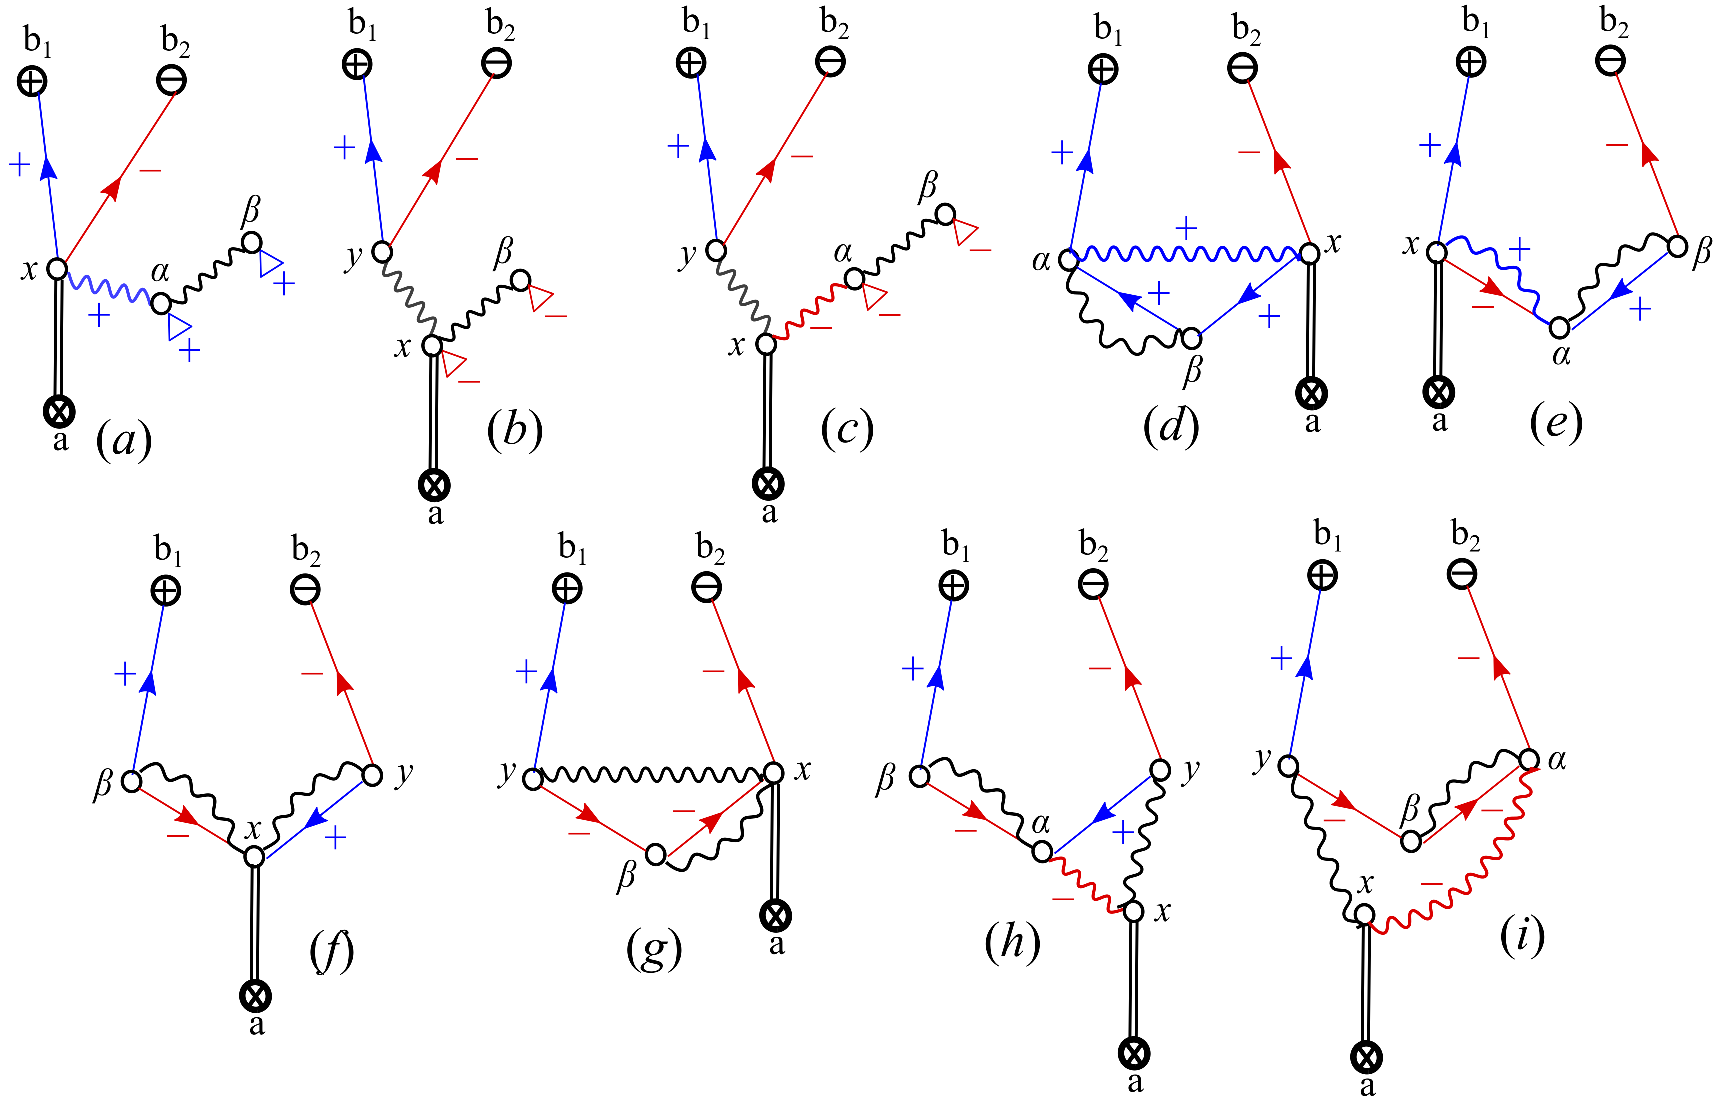
\includegraphics[width=12.5cm]{Aho3.pdf}} 
\ee
For conciseness, we do not draw the coefficients of these graphs. The graphs in \eqref{Aho3} are not yet normal regular, but it is easy to see that after applying $\cal O_{dot}$ to them, all the resulting graphs are of scaling order $\ge 4$. Thus we have obtained the following third order $T$-expansion  
\begin{align} 
 T_{\fa,\fb_1\fb_2} &=  m  \Theta_{\fa\fb_1}\overline G_{\fb_1\fb_2} 
  +  (\AT^{(>3)})_{\fa,\fb_1\fb_2} + (\QT^{(3)})_{\fa,\fb_1\fb_2},\label{thirduniversal}
 \end{align}
 where $ \QT^{(3)}:= \cal Q_{T,3} + \QT^{(2)}$.
 
 \subsection{Fourth order $T$-expansion}
Next we can perform local and global expansions to the graphs in $\AT^{(>3)}$ to construct the fourth order $T$-expansion. Since the expression of the fourth order $T$-expansion is rather lengthy and does not help our proof, we will not give its explicit form in this paper. Instead, we will describe the expansions of several typical graphs to show that we actually have $\Sdelta^{(4)}=0$ in the current setting where $H$ has complex Gaussian entries.  

First, the graphs (a), (b), (c) in \eqref{Aho3} all have two light weights in them. Taking graph (a) as an example, we apply the weight expansion in Definition \ref{Owx} to the weight $G_{\beta\beta}-m$ and get that
\begin{align*}
%& \sum_{\al,\gamma_1,\gamma_2} \Theta_{x\al}  S^+_{\al\gamma_1}s_{\gamma_1\gamma_2} (G_{\gamma_1\gamma_1}-m)(G_{\gamma_2\gamma_2}-m) G_{\al y}\overline G_{\al y'}  \\
%&=m  \sum_{x,\al,\beta,\gamma} \Theta_{\fa x}  S^+_{x\al}s_{\al\beta} s_{\beta\gamma}(G_{\al\al}-m)(G_{\beta\beta}-m)(G_{\gamma\gamma}-m) G_{x\fb_1}\overline G_{x\fb_2} \tag{a1}\\
%& + m \sum_{x,\al,\beta,\gamma_1,\gamma_2} \Theta_{\fa x}  S^+_{x\al}s_{\al\beta} S^+_{\beta\gamma_1}s_{\gamma_1\gamma_2}(G_{\al\al}-m)(G_{\gamma_1\gamma_1}-m)(G_{\gamma_2\gamma_2}-m) G_{x\fb_1}\overline G_{x\fb_2} \\
%	& +m\sum_{x,\al,\beta,\gamma} \Theta_{\fa x}  S^+_{x\al}s_{\al\beta} s_{\beta \gamma}G_{\gamma \beta} G_{\al\gamma}G_{\beta \al}  G_{x\fb_1}\overline G_{x\fb_2} \tag{a2}\\
%	&  +m \sum_{x,\al,\beta,\gamma_1,\gamma_2} \Theta_{\fa x}  S^+_{x\al}s_{\al\beta} S^+_{\beta\gamma_1}s_{\gamma_1\gamma_2} G_{\gamma_2\gamma_1} G_{\al\gamma_2}G_{\gamma_1\al} G_{x\fb_1}\overline G_{x\fb_2}  \\
& \sum_{x,\al,\beta} \Theta_{\fa x}  S^+_{x\al}s_{\al\beta} (G_{\al\al}-m)(G_{\beta\beta}-m) G_{x\fb_1}\overline G_{x\fb_2}=  \cal Q_a\\
& + m^{-1} \sum_{x,\al,\gamma_1,\gamma_2} \Theta_{\fa x} S^+_{x\al}S^+_{\al\gamma_1}s_{\gamma_1\gamma_2}(G_{\al\al}-m)(G_{\gamma_1\gamma_1}-m)(G_{\gamma_2\gamma_2}-m) G_{x\fb_1}\overline G_{x\fb_2} \tag{a1}\\
& +m^{-1} \sum_{x,\al, \gamma_1,\gamma_2} \Theta_{\fa x}  S^+_{x\al}S^+_{\al \gamma_1}s_{\gamma_1\gamma_2} G_{\gamma_2\gamma_1} G_{\al\gamma_2}G_{\gamma_1\al} G_{x\fb_1}\overline G_{x\fb_2} \tag{a2} \\
%&+m\sum_{\al,\gamma_1,\gamma_2,\gamma_3} \Theta_{x\al}  S^+_{\al\gamma_1}s_{\gamma_1\gamma_2} s_{\gamma_2\gamma_3}(G_{\gamma_1\gamma_1}-m)   G_{\gamma_3\gamma_2}  G_{\al \gamma_3}G_{\gamma_2 y}\overline G_{\al y'}\\
& + m^{-1} \sum_{x,\al,\gamma_1,\gamma_2} \Theta_{\fa x}  S^+_{x\al}S^+_{\al \gamma_1}s_{\gamma_1\gamma_2} (G_{\al\al}-m) G_{\gamma_2\gamma_1}  G_{x \gamma_2}G_{\gamma_1 \fb_1}\overline G_{x \fb_2} \tag{a3}  \\
%&+m\sum_{\al,\gamma_1,\gamma_2,\gamma_3} \Theta_{x\al}  S^+_{\al\gamma_1}s_{\gamma_1\gamma_2} s_{\gamma_2\gamma_3}(G_{\gamma_1\gamma_1}-m)  G_{\gamma_3\gamma_2}   G_{\al y}\overline G_{\al \gamma_2}\overline G_{\gamma_3 y'} \\
& +m^{-1} \sum_{x,\al, \gamma_1,\gamma_2} \Theta_{\fa x}  S^+_{x\al} S^+_{\al\gamma_1}s_{\gamma_1\gamma_2} (G_{\al\al}-m) G_{\gamma_2\gamma_1}  G_{x\fb_1}\overline G_{x \gamma_1} \overline G_{\gamma_2 \fb_2} , \tag{a4}
 \end{align*}
where we used \eqref{iden_S+} in the derivation, and $\cal Q_a$ is a sum of $Q$-graphs. In \eqref{Aho41}, we draw the four graphs (a1)--(a4), where for conciseness we do not draw the coefficients of them. 
\be  \label{Aho41} 
\parbox[c]{0.8\linewidth}{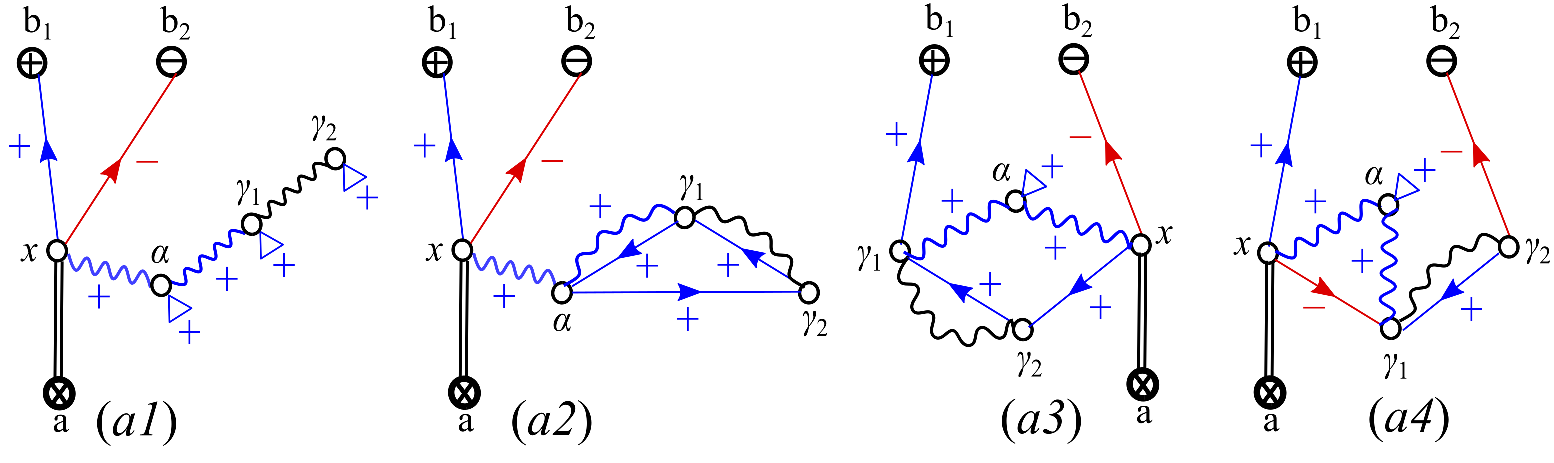
\includegraphics[width=12.5cm]{Aho41.pdf}} 
\ee
The graphs in \eqref{Aho41} are not yet normal regular, but it is easy to see that after applying $\cal O_{dot}$ to them, all the resulting graphs are of scaling order $\ge 5$.   
%All the non-$Q$ graphs have scaling order $\ge 5$ after applying the dotted edge partition in Definition \ref{dot-def}. One can check that all these graphs have scaling order $\ge 5$, no matter how we assign the dotted edge partition for the $G$ edges.
Similarly, we can check that applying the weight expansion to the light weights in graphs (b) and (c) of \eqref{Aho3} will give graphs of scaling order $\ge 5$. 

Second, the graphs (d), (g) and (i) in \eqref{Aho3} all have an atom $\beta$ connected with two matched edges of the same charge. Taking graph (i) as an example, we apply the $GG$ expansion in Definition \ref{GG-def} to the two edges connected with $\beta$, and get that 
\begin{align*}
& 	|m|^2 \sum_{x,y,\al,\beta} \Theta_{\fa x} s_{xy}  S^-_{x\al} s_{\al\beta}\overline G_{\beta\al} \overline G_{y\beta} G_{y\fb_1}\overline G_{\al\fb_2}=\cal Q_i\\
%& |m|^2 \sum_{\al,\beta,\gamma_1,\gamma_2} \Theta_{x\al} s_{\al\beta}  S^-_{\al\gamma_1} s_{\gamma_1\gamma_2}\overline G_{\beta \gamma_2} \overline G_{\gamma_2\gamma_1}  G_{\beta y}\overline G_{\gamma_1 y'} \\
& + |m|^2 \overline m\sum_{x,y,\al,\beta} \Theta_{\fa x} s_{xy}  S^-_{x\al} s_{\al\beta}S^-_{\al\beta}\overline G_{y\al} G_{y\fb_1}\overline G_{\al\fb_2} \tag{i1}\\
%&\cor + |m|^2 \overline m\sum_{\al,\beta,\gamma_1,\gamma_2, \gamma_3} \Theta_{x\al} s_{\al\beta}  S^-_{\al\gamma_1} s_{\gamma_1\gamma_2} s_{\gamma_2\gamma_3} (\overline G_{\gamma_3\gamma_3}-\overline m )\overline G_{\beta \gamma_2} \overline G_{\gamma_2\gamma_1}  G_{\beta y}\overline G_{\gamma_1 y'} \tag{i2}\\
%&\cor + |m|^2 \overline m\sum_{\al,\beta,\gamma_1,\gamma_2, \gamma_3,\gamma_4} \Theta_{x\al} s_{\al\beta}  S^-_{\al\gamma_1} s_{\gamma_1\gamma_2} S^-_{\gamma_2\gamma_3}s_{\gamma_3\gamma_4} (\overline G_{\gamma_4\gamma_4}-\overline m )\overline G_{\beta \gamma_3} \overline G_{\gamma_3\gamma_1}  G_{\beta y}\overline G_{\gamma_1 y'} \tag{i3}\\
&  + m\sum_{x,y,\al, \gamma_1,\gamma_2} \Theta_{\fa x} s_{xy}  S^-_{x\al} S^-_{\al \gamma_1}s_{\gamma_1\gamma_2} (\overline G_{\gamma_2\gamma_2}-\overline m ) \overline G_{\gamma_1\al} \overline G_{y \gamma_1} G_{y\fb_1}\overline G_{\al \fb_2} \tag{i2}\\
%&\cor + |m|^2\overline m \sum_{x,y,\al,\beta,\gamma_1} \Theta_{\fa x} s_{xy}  S^-_{x\al} s_{\al\beta}   s_{\beta\gamma_1}  (\overline G_{\beta\beta}-\overline m ) \overline G_{y \gamma_1} \overline G_{\gamma_1\al}  G_{y \fb_1}\overline G_{\al \fb_2} \\
%&\cor + |m|^2 \overline m\sum_{x,y,\al,\beta, \gamma_1,\gamma_2} \Theta_{\fa x} s_{xy}  S^-_{x\al} s_{\al\beta} S^-_{\beta\gamma_1}s_{\gamma_1\gamma_2} (\overline G_{\gamma_1\gamma_1}-\overline m )\overline G_{y \gamma_2} \overline G_{\gamma_2\al}  G_{y\fb_1}\overline G_{\al\fb_2} \\
&  +  m\sum_{x,y,\al, \gamma_1,\gamma_2} \Theta_{\fa x} s_{xy}  S^-_{x\al}S^-_{\al\gamma_1}s_{\gamma_1\gamma_2} (\overline G_{\gamma_1\gamma_1}-\overline m )\overline G_{\gamma_2\al} \overline G_{y \gamma_2}  G_{y\fb_1}\overline G_{\al\fb_2} \tag{i3}\\
%&\cor + |m|^2\overline m \sum_{\al,\beta,\gamma_1,\gamma_2,\gamma_3} \Theta_{x\al} s_{\al\beta}  S^-_{\al\gamma_1} s_{\gamma_1\gamma_2}s_{\gamma_2\gamma_3} |G_{\beta \gamma_2}|^2 \overline G_{\gamma_3\gamma_1}  G_{\gamma_3 y}\overline G_{\gamma_1 y'} \\
%&\cor + |m|^2 \overline m\sum_{\al,\beta,\gamma_1,\gamma_2,\gamma_3,\gamma_4} \Theta_{x\al} s_{\al\beta}  S^-_{\al\gamma_1} s_{\gamma_1\gamma_2}S^-_{\gamma_2 \gamma_3}s_{\gamma_3\gamma_4} \overline G_{\beta \gamma_3} \overline G_{\gamma_4\gamma_1}   G_{\beta \gamma_3}G_{\gamma_4 y}\overline G_{\gamma_1 y'}\\
& +  m\sum_{x,y,\al, \gamma_1,\gamma_2} \Theta_{\fa x} s_{xy}  S^-_{x\al} S^-_{\al\gamma_1}s_{\gamma_1\gamma_2} |G_{y \gamma_1}|^2 \overline G_{\gamma_2\al}   G_{\gamma_2 \fb_1}\overline G_{\al \fb_2} \tag{i4}\\
%&\cor + |m|^2\overline m \sum_{\al,\beta,\gamma_1,\gamma_2,\gamma_3} \Theta_{x\al} s_{\al\beta}  S^-_{\al\gamma_1} s_{\gamma_1\gamma_2}s_{\gamma_2\gamma_3}\overline G_{\beta \gamma_2} \overline G_{\gamma_3\gamma_1} G_{\beta y}\overline G_{\gamma_1 \gamma_3} \overline G_{\gamma_2 y'} \\
%&\cor+ |m|^2 \overline m\sum_{\al,\beta,\gamma_1,\gamma_2,\gamma_3,\gamma_4} \Theta_{x\al} s_{\al\beta}  S^-_{\al\gamma_1} s_{\gamma_1\gamma_2}S^-_{\gamma_2 \gamma_3}s_{\gamma_3\gamma_4} \overline G_{\beta \gamma_3} \overline G_{\gamma_4\gamma_1}   G_{\beta y}\overline G_{\gamma_1 \gamma_4}\overline G_{\gamma_3 y'} +\cal Q_i \\
& +  m\sum_{x,y,\al,\gamma_1,\gamma_2} \Theta_{\fa x} s_{xy}  S^-_{x\al}  S^-_{\al\gamma_1}s_{\gamma_1\gamma_2} \overline G_{y \gamma_1}\overline G_{\al \gamma_2}  \overline G_{\gamma_2\al}  G_{y\fb_1}\overline G_{\gamma_1 \fb_2} , \tag{i5}
\end{align*}
where we used the complex conjugate of \eqref{iden_S+} in the derivation, and $\cal Q_i$ is a sum of $Q$-graphs. In \eqref{Aho42}, we draw the five graphs (i1)--(i5), where for conciseness we do not draw the coefficients of the graphs.  
% All the non-$Q$ graphs have scaling order $\ge 5$ after applying the dotted edge partition in Definition \ref{dot-def}. Here we draw the graphs (i1)-(i5) on the right-hand side, where for conciseness we do not draw the coefficients of the graphs. One can check that all these graphs have scaling order $\ge 5$, no matter how we assign the dotted edge partition for the $G$ edges. 
\be  \label{Aho42} 
\parbox[c]{0.85\linewidth}{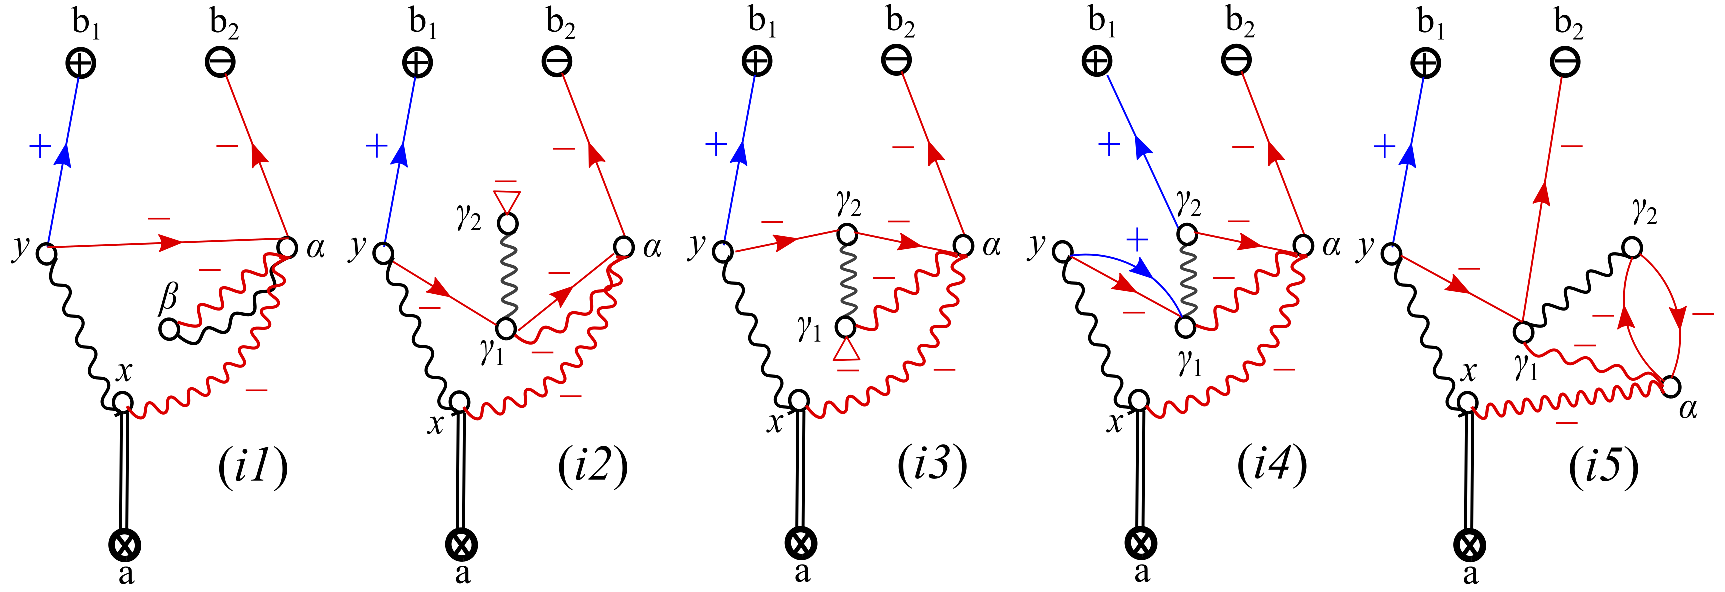
\includegraphics[width=13.5cm]{Aho42.pdf}} 
\ee
The graphs in \eqref{Aho42} are not yet normal regular, but it is easy to see that after applying $\cal O_{dot}$ to them, all the resulting graphs are of scaling order $\ge 5$. Similarly, we can check that applying the $GG$ expansion to the two $G$ edges connected with atom $\beta$ in the graphs (d) and (g) of \eqref{Aho3} will give graphs of scaling order $\ge 5$. 

Finally, the graphs (e), (f) and (h) of \eqref{Aho3} only contain degree 2 atoms connected with two matched edges of opposite charges, but not all atoms in them are standard neutral, such as the atom $x$ in (f) and the atom $\al$ in (e) and (h). Taking graph (f) as an example, we apply the $G\overline G$ expansion in Definition \ref{GGbar-def} to the two edges connected with atom $x$, and get that 
\begin{align*}
	&|m|^2 \sum_{x,y,\beta} \Theta_{\fa x} s_{xy} s_{x\beta}\overline G_{\beta x}  G_{y x}G_{\beta\fb_1}\overline G_{y\fb_2}= \cal Q_f\\
%& |m|^2 \sum_{\al,\beta, \gamma_2} \Theta_{x\al} s_{\al\beta} s_{\al \gamma_2}\overline G_{\gamma_2\al}  G_{\beta \al}G_{\gamma_2 y}\overline G_{\beta y'}  \\
&+ |m|^4 \sum_{x,y,\al,\beta } \Theta_{\fa x} s_{xy} s_{x\beta}s_{x\al}\overline G_{\beta\al}  G_{y \al}G_{\beta\fb_1}\overline G_{y\fb_2} \tag{f1}\\
&+ |m|^2 m \sum_{x,y,\al,\beta} \Theta_{\fa x} s_{xy} s_{x\beta}s_{x\al} (G_{\al\al}-m)\overline G_{\beta x}  G_{y x}G_{\beta \fb_1}\overline G_{y\fb_2} \tag{f2}\\
&+ |m|^2 m \sum_{x,y,\al,\beta} \Theta_{\fa x} s_{xy} s_{x\beta}s_{x\al} (\overline G_{xx}-\overline m)\overline G_{\beta\al}  G_{y\al}G_{\beta\fb_1}\overline G_{y\fb_2} \tag{f3}\\
&+ |m|^2 m\sum_{x,y,\al,\beta } \Theta_{\fa x} s_{xy} s_{x\beta}s_{x\al} G_{y\al}  |G_{\beta x}|^2 G_{\al\fb_1}\overline G_{y\fb_2}   \tag{f4}\\
&+ |m|^2 m\sum_{x,y,\al,\beta} \Theta_{\fa x} s_{xy} s_{x\beta}s_{x\al}\overline G_{\beta x}  |G_{y \al}|^2  G_{\beta \fb_1} \overline G_{x\fb_2} , \tag{f5}
\end{align*}
where $\cal Q_f$ is a sum of $Q$-graphs. In \eqref{Aho43}, we draw the five graphs (f1)--(f5), where for conciseness we do not draw the coefficients of them. % One can check that all the graphs (f2)-(f5) have scaling order $\ge 5$, no matter how we assign the dotted edge partition for the $G$ edges. 
 \be  \label{Aho43} 
\parbox[c]{0.85\linewidth}{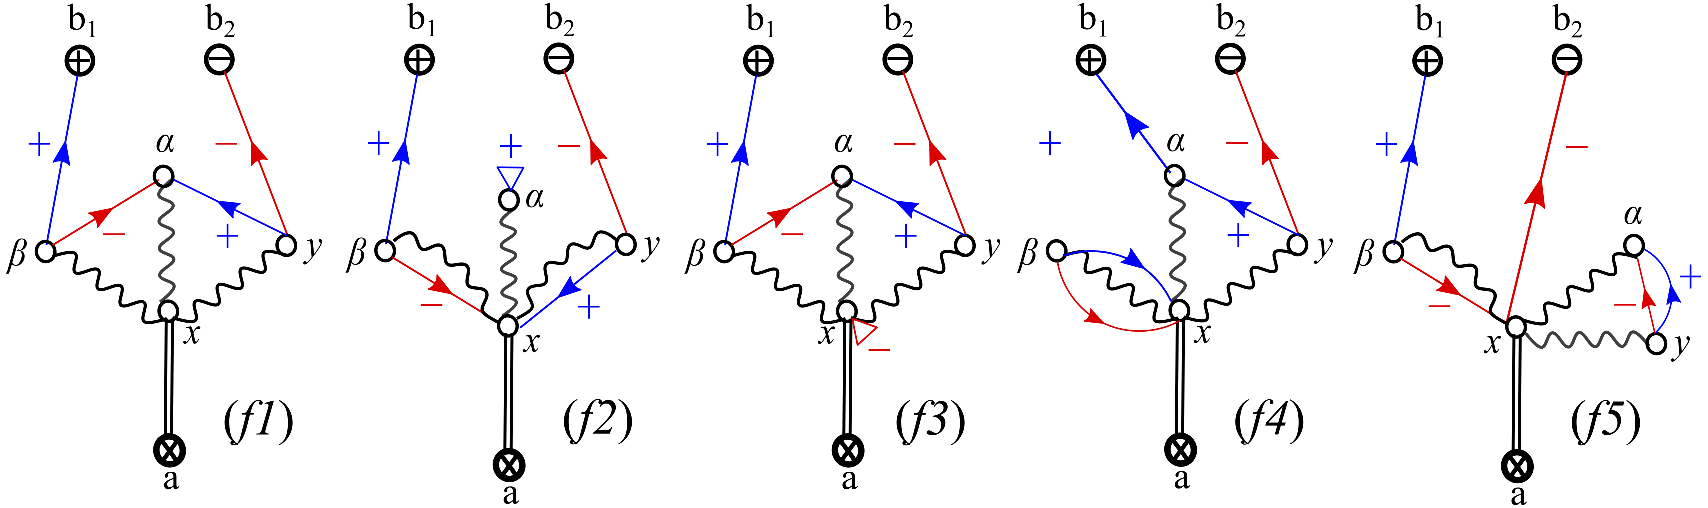
\includegraphics[width=13.5cm]{Aho43.pdf}} 
\ee
Here the graph (f1) is the main term, while the graphs (f2)--(f5) all give graphs of scaling order $\ge 5$ after a dotted edge partition $\cal O_{dot}$.  Next we apply a global expansion to (f1), that is, we replace $|m|^2\sum_{\al}s_{x\al}G_{y\al}\overline G_{\beta\al }$ with the second order $T$-expansion in \eqref{seconduniversal}:
\begin{align*}
&	|m|^4 \sum_{x,y,\al,\beta } \Theta_{\fa x} s_{xy} s_{x\beta}s_{x\al}\overline G_{\beta\al}  G_{y \al}G_{\beta\fb_1}\overline G_{y\fb_2}  =  |m|^2 \sum_{x,y,\beta} \Theta_{\fa x} s_{xy} s_{x\beta}(\QT^{(2)})_{y\beta, x}  G_{\beta \fb_1}\overline G_{y\fb_2} \\
&+ |m|^2 m \sum_{x,y,\beta} \Theta_{\fa x} s_{xy} s_{x\beta}\Theta_{xy} \overline G_{\beta y}  G_{\beta\fb_1}\overline G_{y\fb_2} \tag{f1.1}\\
&+|m|^2 m\sum_{x,y,\beta ,\gamma_1,\gamma_2} \Theta_{\fa x} s_{xy} s_{x\beta}\Theta_{x\gamma_1} s_{\gamma_1\gamma_2} (G_{\gamma_2\gamma_2}-m) \overline G_{\beta \gamma_1}  G_{y \gamma_1}G_{\beta \fb_1}\overline G_{y\fb_2} \tag{f1.2}\\
&+|m|^2 m\sum_{x,y,\beta ,\gamma_1,\gamma_2} \Theta_{\fa x} s_{xy} s_{x\beta}\Theta_{x \gamma_1} s_{\gamma_1\gamma_2} (\overline G_{\gamma_1\gamma_1}-\overline m) \overline G_{\beta \gamma_2}  G_{y \gamma_2}G_{\beta \fb_1}\overline G_{y \fb_2}. \tag{f1.3}
\end{align*}
We need to further apply a $Q$-expansion to the first term on the right-hand side. In \eqref{Aho44}, we draw the three graphs (f1.1)--(f1.3), where for conciseness we do not draw the coefficients of them. It is easy to see that after applying $\cal O_{dot}$ to these graphs, all the resulting graphs are of scaling order $\ge 5$.  
%The graphs (f1.1)-(f1.3) are all of scaling order $\ge 5$ after applying the dotted edge partition in Definition \ref{dot-def}. Here we draw these graphs, where for conciseness we do not draw the coefficients of the graphs. One can check that all the graphs (f1.1)-(f1.3) have scaling order $\ge 5$, no matter how we assign the dotted edge partition for the $G$ edges. 
 \be  \label{Aho44} 
\parbox[c]{0.7\linewidth}{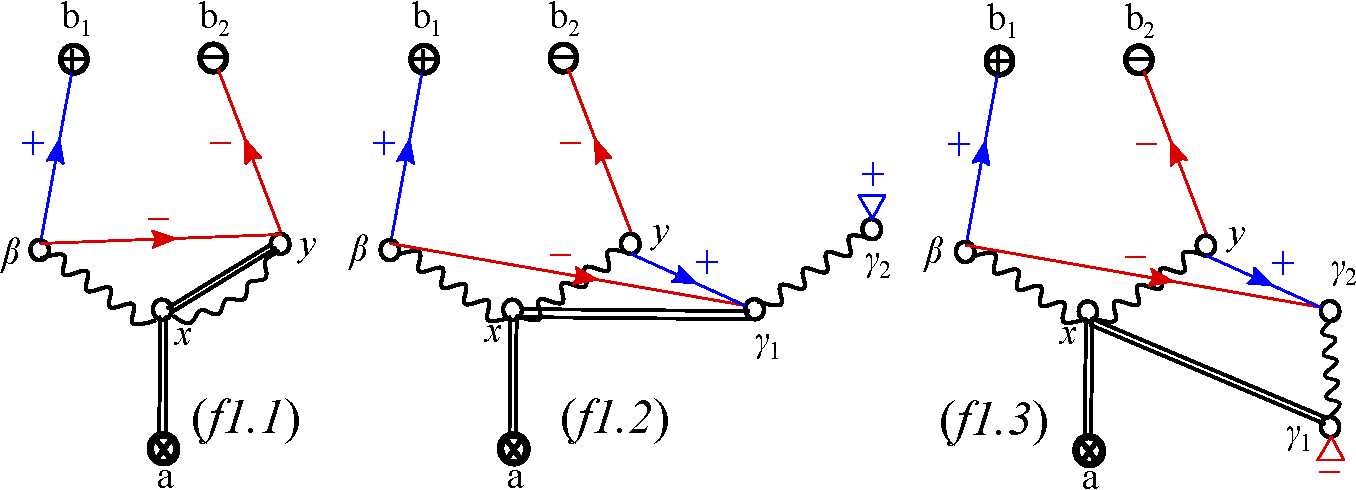
\includegraphics[width=11cm]{Aho44.pdf}} 
\ee
Similarly, we can check that after applying the $G\overline G$ expansion to the two $G$ edges connected with atom $\al$ in graphs (e) and (h) of \eqref{Aho3} and then applying a global expansion, we will get graphs of scaling order $\ge 5$. 
    
To summarize, we have found that in the fourth order $T$-expansion, the fourth order $\self$ $\Sele_4$ vanishes.  
 

\subsection{Examples of graphs in $\self$ $\Sele_6$}
In this subsection, we use some examples to show that the 6th order $\self$ actually contains non-trivial graphs. Hence, unlike $\Sele_4$, its sum zero property \eqref{weaz} is not trivial anymore. We remark there are hundreds of ways to get graphs in $\Sele_6$, and we are not trying to exhaust all of them. %{\cor emphasize that this section is mainly to give some examples of the $\self$}
   
First, if we assign the dotted edge partition such that the two internal $G$ edges in (d)--(i) of \eqref{Aho3} are diagonal, then we will get sixth order graphs. For example, for the graph (d) of \eqref{Aho3}, we assign dotted edges $\delta_{x\beta}$ and $\delta_{\al \beta}$, and then replace the two weights $G_{xx}^2$ with $m^2$; for the graph (h), we assign dotted edges $\delta_{y\al}$ and $\delta_{\al\beta}$, and then replace the two weights $|G_{yy}|^2$ with $|m|^2$. Then we get the following two graphs:
\be  \label{Aho61} 
\parbox[c]{0.3\linewidth}{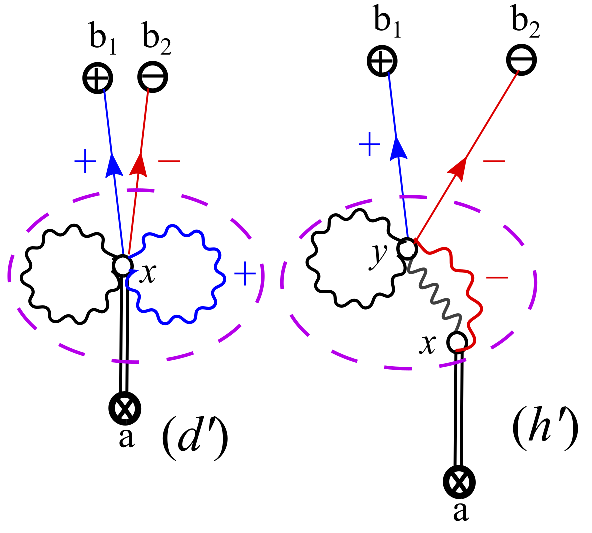
\includegraphics[width=5cm]{Aho61.pdf}} 
\ee
%Second, for graph (a3) in \eqref{Aho41}, if we add a dotted edge between $\gamma_2$ and $\gamma_3$, and replace the weight $G_{\gamma_2\gamma_2}$ with $m$, we get graph (a3') in the above figure. Then applying the $GG$ expansion in Definition \ref{GG-def} to the edges $G_{\gamma_2\gamma_3}G_{\gamma_3\gamma_2}$ and replacing them the leading term $m^2 S^+_{\gamma_3\gamma_3}$, we get graph (a3'') in the above figure \eqref{Aho61}. 
%The graphs produce the following deterministic graphs in 
Inside the purple dashed circles are two deterministic graphs in $(\Sele_6)_{xy}$ (except for the coefficients):
$$(d'): \ m^2 \delta_{xy} s_{xx}S^+_{xx},\quad (h'):\ |m|^4 s_{yy}s_{xy} S^-_{xy}. $$ % \quad (a3''): \  \delta_{\al\beta} \sum_{\gamma_1,\gamma_2} S^-_{\al\gamma_1} (s_{\gamma_1\gamma_2})^2 S^+_{\gamma_1,\gamma_2}.$$
Note that (d$'$) is a diagonal graph, i.e., $x$ and $y$ are connected by a dotted edge. Its value at $x=y$ is of order $W^{-2d}$, while the term $L^\tau W^{-(l-4)d/2}B_{0x}^2$ in \eqref{4th_property0} with $l=6$ is of order $L^\tau W^{-3d}$ at $x=0$; this is why \eqref{4th_property0} also contains the term $L^\tau W^{-(l-2)d/2}\mathbf 1_{x=0}$.
%There are some coefficients associated with these graphs, but we do not keep track of them.
 
As the second example, in the graph (i4) of \eqref{Aho42}, if we assign a dotted edge $\delta_{\al\gamma_2}$, replace the weight $\overline G_{\al\al}$ with $\overline m$, replace the $T$-variable $|m|^2\sum_{y}s_{xy}|G_{y\gamma_1}|^2$ with $|m|^2\Theta_{x\gamma_1}$ in a global expansion, and rename $\al$ as $y$, we then get the graph (i4$'$) in \eqref{Aho62}. In the graph (i5) of \eqref{Aho42}, if we assign a dotted edge $\delta_{y \gamma_1}$, replace the weight $\overline G_{yy}$ with $\overline m$, and replace the two edges  $\overline G_{\al\gamma_2}\overline G_{\gamma_2\al}$ with $\overline m^2 S^-_{\al\gamma_2}$ in the $GG$ expansion, then we get the graph (i5$'$) in \eqref{Aho62}.
    \be  \label{Aho62} 
\parbox[c]{0.4\linewidth}{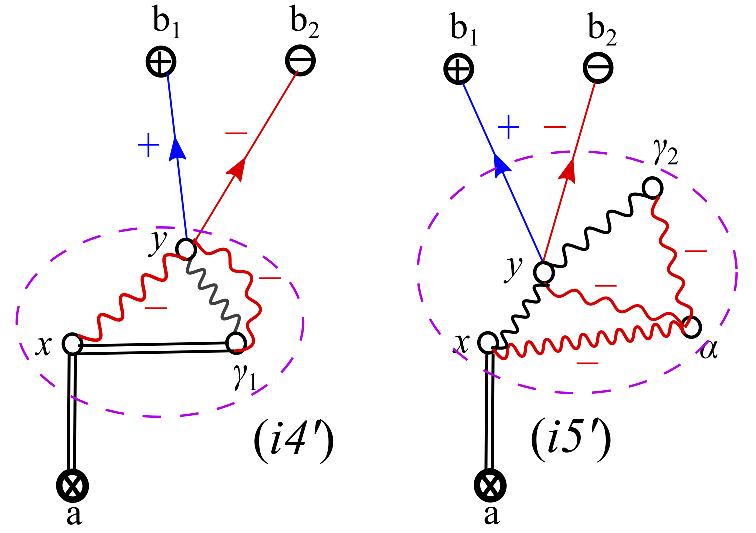
\includegraphics[width=6.5cm]{Aho62.pdf}} 
\ee
Inside the purple dashed circles are two deterministic graphs in $(\Sele_6)_{xy}$ (except for the coefficients):
$$  (i4'):\ |m|^2 S^-_{xy}\sum_{\gamma_1}s_{y\gamma_1}S^-_{y\gamma_1} \Theta_{x\gamma_1}, \quad (i5'): \ |m|^2\overline m^2 s_{xy} \sum_{\al,\gamma_2}S^-_{x\al} S^-_{y\al} S^-_{\al \gamma_2}s_{y\gamma_2}.$$
%There are some coefficients associated with these graphs, but we do not keep track of them.

As the last example, in the graph (f4) of \eqref{Aho43}, if we assign a dotted edge $\delta_{y\al}$, replace the weight $  G_{yy}$ with $ m$, and replace the $T$-variable $|m|^2\sum_{\beta}s_{x\beta}|G_{\beta x}|^2$ with a $|m|^2\Theta_{xx}$ edge in a global expansion, then we get the graph (f4$'$) in \eqref{Aho63}. In the graph (f1.1) of \eqref{Aho44}, if we assign a dotted edge $\delta_{y\beta}$ and replace the weight $\overline G_{yy}$ with $\overline m$, then we get the graph (f1.1$'$) in \eqref{Aho63}.
    \be  \label{Aho63} 
\parbox[c]{0.3\linewidth}{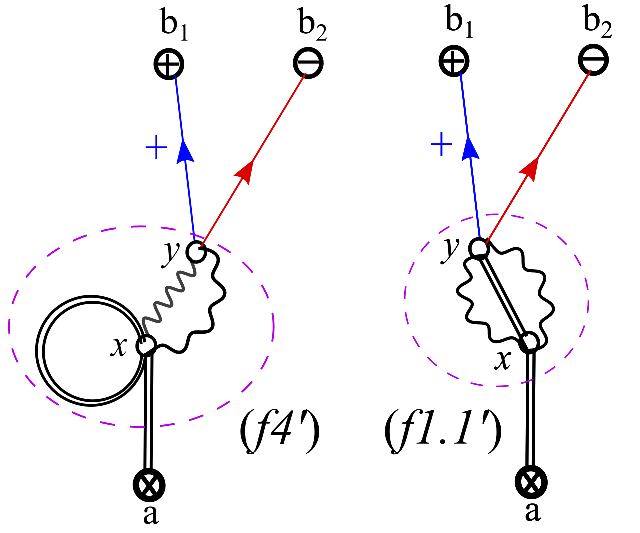
\includegraphics[width=5cm]{Aho63.pdf}} 
\ee
Inside the purple dashed circles are two deterministic graphs in $(\Sele_6)_{xy}$ (except for the coefficients):
$$ \quad (f4'):\   |m|^2 m^2 \Theta_{xx}(s_{xy})^2 , \quad (f1.1'): \  |m|^4(s_{xy})^2\Theta_{xy}.$$
%There are some coefficients associated with these graphs, but we do not keep track of them.

 % \begin{remark}\label{decompose rmk}
% Setting $y=y'$ in \eqref{seconduniversal} and \eqref{thirduniversal}, we obtain the second and third order $T$-expansions of $T_{xy}$:
%\be\label{mlevelT0}
%\begin{split}
% T_{xy} \equiv T_{x,yy}&= m \overline G_{yy} \left[\Theta_{xy} + \left(\Theta \Sdelta^{(2)} \Theta\right)_{xy}\right]
%  +  (\AT^{(>2)})_{xy} + (\QT^{(2)})_{xy} \\ %+ \OO(L^{-D})
%  &= m \overline G_{yy} \left[\Theta_{xy} + \left(\Theta \Sdelta^{(3)} \Theta\right)_{xy}\right]
%  +  (\AT^{(>3)})_{xy} + (\QT^{(3)})_{xy} .
%  \end{split}
%\ee
%%where as a convention we set $\Sdelta^{(3)}  =\Sdelta^{(2)}  =0$. 
%In order to get the expansions in \eqref{mlevelTgdefintro}, we write $\overline G_{yy}=\overline m + (\overline G_{yy}-\overline m)$, and regard 
%$$m (\overline G_{yy}-\overline m)  \Theta_{xy}   = m \sum_\al \delta_{\al y}(\overline G_{\al\al}-\overline m)  \Theta_{x\al}  $$
%as a term in $(\PT^{(2)})_{xy}$ and $(\PT^{(3)})_{xy}$. 
%More generally, in $n$-th order $T$-expansions, we will regard 
%$$m (\overline G_{yy}-\overline m) \left[\Theta_{xy} + \left(\Theta \Sdelta^{(n)} \Theta\right)_{xy}\right] = m \sum_\al \delta_{\al y}(\overline G_{\al\al}-\overline m) \left[\Theta_{x\al} + \left(\Theta \Sdelta^{(n)} \Theta\right)_{x\al}\right]$$
%as a term in $(\PTn)_{xy}$.
%%and abbreviated  $(\cal A^{(>2)}_{ho})_{xy}\equiv (\cal A^{(>2)}_{ho})_{x,yy}$ and $\cal{Q}^{(2)}_{xy}\equiv \cal {Q}^{(2)}_{x,yy}$.
% \end{remark}

  
 
  
%------------- some examples of 4th and 6th order $T$-expansions ------------------
% \begin{example}
%For the fourth order $T$-expansion of the $T$-variable $T_{\fa\fb}=|m|^2\sum_x s_{\fa x}|G_{x\fb}|^2$, we have the following types of graphs:
%\begin{itemize}
%\item Deterministic graphs:
%\begin{align*} 
%(S_{\Delta}^{(4)})_{xy}(z) &=|m(z)|^2 \re\left( |m(z)|^4  + \frac{2m^4(z)}{1-m^2(z)} \right) \Big[ \sum_{\beta}\left(\mathbb E|h_{x\beta}|^4 - 2s_{x\beta}^2\right)\Big]s_{xy} \\
%&+ 2|m(z)|^2 \re(m^2(z)) \left(\mathbb E|h_{xy}|^4 - 2s_{xy}^2\right) .
%\end{align*}
%Note that for complex Gaussian, we have $\mathbb E|h_{x\beta}|^4 - 2s_{x\beta}^2=0$, hence we will not be able to discover this term in this case.
%
%\item Some $(\fa,\fb)$-recollision graphs, for example,
%\begin{align*}
%&\Theta_{\fa \fb}|G_{\fb\fb}|^2, \quad   \Theta_{\fa \fa}|G_{\fa\fb}|^2, \quad |m|^2 \sum_{x,\al,\beta}\Theta_{\fa x} s_{x\al}s_{x\beta}s_{x\fb} |G_{\al \fb}|^2 |G_{\beta\fb}|^2, \quad |m|^2 \sum_{x,\al,\beta}\Theta_{\fa x} s_{x\al}s_{x\beta}s_{x\fb} |G_{\fb \fb}|^2 |G_{\al\beta}|^2 .
%%& \re\left( m \sum_{x,\al}\Theta_{\fa x}s_{x\al}s_{x\fb} G_{\fb\fb}|G_{\al \fb}|^2\right), \quad \re\left( m \sum_{x,\al}\Theta_{\fa x}s_{x\al}s_{x\fb} \overline G_{\fb\fb}G_{\al \fb} G_{\fb\al} \right), \\ 
%%&\re\left( m^2 \sum_{x,y,\al,\beta}\Theta_{\fa x}S^+_{xy}s_{x\fb}s_{y\al} s_{y\beta}|G_{\fb\fb}|^2 G_{\beta\al}G_{\al \beta}\right),  \quad \re\left( m^2 \sum_{x,y,\al,\beta}\Theta_{\fa x}S^+_{xy}s_{x\al}s_{y\beta}s_{y\fb} G_{\fb\fb}\overline G_{\al \fb} G_{\al\beta}G_{\beta\fb}\right).
%\end{align*}
% 
%
% \item Some higher order terms involve recollisions of indices, such as,
% $$\sum_{x,\al,\beta}\Theta_{\fa x}s_{x\al }s^2_{x\beta}\overline G_{\beta\beta} G_{\beta\al}G_{\al\otimes}\overline G_{\beta\otimes}.$$
% Some other higher order are typically expansion the following ``diamond" graphs:
% \begin{align}
%& \re\left(m^2 \sum_{x,\al_1,\al_2,\al_3} \Theta_{\fa x}s_{x\al_1}s_{x\al_2}s_{x\al_3}\overline G_{\al_1 \otimes}G_{\al_1\al_2}G_{\al_2 \al_3}G_{\al_3\otimes}\right), \label{example1}\\ 
%&  \sum_{x,\al_1,\al_2,\al_3} \Theta_{\fa x} s_{x\al_1}s_{x\al_2}s_{x\al_3}\overline G_{\al_2\al_1}\overline G_{\al_1 \otimes}G_{\al_2 \al_3}G_{\al_3\otimes} ,\label{example2}\\
%&  \sum_{x,\al_1,\al_2,\al_3} \Theta_{\fa x}s_{x\al_1}s_{x\al_2}s_{x\al_3}\overline G_{\al_1 \otimes} G_{\al_1\al_2}\overline G_{\al_3\al_2} G_{\al_3\otimes} .\label{example3}
% \end{align}
% \be  \nonumber 
%\parbox[c]{0.64\linewidth}{\includegraphics[width=\linewidth]{4th1.png}} 
%\ee
% Or there are some similar versions with $S^+$ edges
%  \begin{align*}
%& \re\left(m^2 \sum_{x,y,\al_1,\al_2,\al_3} \Theta_{\fa x}S^+_{xy}s_{x\al_1}s_{y\al_2}s_{y\al_3}\overline G_{\al_1 \otimes}G_{\al_1\al_2}G_{\al_2 \al_3}G_{\al_3\otimes}\right),\\
%& \re\left(m^2 \sum_{x,y,\al_1,\al_2,\al_3} \Theta_{\fa x}S^+_{xy} s_{x\al_1}s_{y\al_2}s_{y\al_3}\overline G_{\al_2\al_1}\overline G_{\al_1 \otimes}G_{\al_2 \al_3}G_{\al_3\otimes} \right),\\
%& \re\left(m^2  \sum_{x,y,\al_1,\al_2,\al_3} \Theta_{\fa x}S^+_{xy} s_{x\al_1}s_{y\al_2}s_{y\al_3}\overline G_{\al_1 \otimes} G_{\al_1\al_2}\overline G_{\al_3\al_2} G_{\al_3\otimes} \right).
% \end{align*}
% For example, the last graph can be drawn as
%  \be  \nonumber 
%\parbox[c]{0.64\linewidth}{\includegraphics[width=3cm]{4th2.png}} 
%\ee
% For example, \eqref{example1} contains a non-neutral atom $\al_2$. Applying the $GG$ expansion in \eqref{Oe2x} below we can get some 5th order terms like
%  \begin{align*}
%& \re\left(m^2 \sum_{x,\al_1,\al_2,\al_3} \Theta_{\fa x}s_{x\al_1}s_{x\al_2}s_{x\al_3}S^+_{\al_1\al_2}\overline G_{\al_1 \otimes}G_{\al_1 \al_3}G_{\al_3\otimes}\right), \\
%& \re\left(m^3 \sum_{x,\al_1,\al_2,\al_3,\beta} \Theta_{\fa x}s_{x\al_1}s_{x\al_2}s_{x\al_3} s_{\al_2\beta}(G_{\al_2\al_2}-m)\overline G_{\al_1 \otimes}G_{\beta\al_2}G_{\beta \al_3}G_{\al_3\otimes}\right).
% \end{align*}
%  \eqref{example3} contains a standard neutral atom $\al_1$. Applying the $\Theta$ expansion \eqref{Otheta}, we can get some 5th order terms like
%  \begin{align*}
%&\sum_{x,\al_2,\al_3} \Theta_{\fa x}\Theta_{x\al_2}s_{x\al_2}s_{x\al_3}\overline G_{\al_2 \otimes} \overline G_{\al_2 \otimes} G_{\al_3\otimes},\\
%&\sum_{x,\al_1,\al_2,\al_3,\beta} \Theta_{\fa x}\Theta_{x\al_1}s_{\al_1\beta} s_{x\al_2}s_{x\al_3}(G_{\beta\beta}-m) \overline G_{\al_1 \otimes} G_{\al_1\al_2}\overline G_{\al_3\al_2} G_{\al_3\otimes}.
% \end{align*}
% 
%  \item Some $Q$-terms, such as
%$$\sum_{x}\Theta_{\fa x}Q_x |G_{x\fb}|^2,\quad \sum_{x,y,\al_1,\al_2, \beta } \Theta_{\fa x}s_{x\al_1}s_{x\al_2} \Theta_{x y}s_{y\beta}Q_\beta\left[ \overline G_{\al_1 \otimes} G_{\al_1\al_2}\overline G_{\beta\al_2} G_{\beta\otimes} \right]$$
% 
% 
%\end{itemize}
%
% \end{example}
% 
% 
% 
% \begin{example}
%We now give some typical 6th order graphs.
%\begin{itemize}
%\item Some possible deterministic graphs, such as
%\begin{align*} 
%%&\sum_{x,\al}\Theta_{\fa x}  s_{x\al}^2  \Theta_{\al\al}\Theta_{\al\fb},\quad  
%& \re\left( \sum_{x,y,\al,\al_1,\al_2}\Theta_{\fa x} S^+_{xy}s_{xy}s_{y\al}s_{y\al_1}s_{y\al_2} \Theta_{\al\fb} \Theta_{\al_1\al_2} \right),\\
%&\sum_{x,\al,\al_1,\al_2,\beta_1,\beta_2}\Theta_{\fa x}s_{x\al}s_{x\al_1}s_{x\al_2}s_{x\beta_1}s_{x\beta_2}\Theta_{\al_1\al_2}\Theta_{\beta_1\beta_2} \Theta_{\al\fb},\quad \sum_{x,\al_1,\al_2,y}\Theta_{\fa x}s_{x\al_1}s_{x\al_2}\Theta_{xy}\Theta_{\al_1 y}\Theta_{\al_2 y}\Theta_{y\fb}.
%\end{align*}
%\be  \nonumber 
%\parbox[c]{0.64\linewidth}{\includegraphics[width=\linewidth]{6th0.png}} 
%\ee
%
%\item Some 6th order graphs involve recollisions of indices, such as,
% $$\re\left(m^3\sum_{x,y,\al_1,\al_2,\beta}\Theta_{\fa x}S^+_{xy}s_{x\al_1}s_{y\al_2}s_{y\al_3}(s^2_{y\beta}G_{\beta\beta}^2) \overline G_{\al_1\otimes} G_{\al_1\al_2}\overline G_{\al_2\al_3}G_{\al_3\otimes} \right).$$
% Some typical 6th order graphs, such as 
% \begin{align*}
%&   \sum_{x,\al_1,\al_2,\al_3,\al_4,\al_5} \Theta_{\fa x}s_{x\al_1}s_{x\al_2}s_{x\al_3}(s_{x\al_4} s_{x\al_5}\Theta_{\al_4\al_5}) \overline G_{\al_1 \otimes}G_{\al_1\al_2}\overline G_{\al_3 \al_2 }G_{\al_3\otimes} , \\ 
%&  \sum_{x,\al_1,\al_2,\al_3,\al_4,\al_5} \Theta_{\fa x} s_{x\al_1}s_{x\al_2}s_{x\al_3}s_{x\al_4} s_{x\al_5} \overline G_{\al_1 \otimes}G_{\al_1\al_2}\overline G_{\al_3 \al_2 }G_{\al_3\al_4} \overline G_{\al_5\al_4} G_{\al_5\otimes}, \\
%& \sum_{x,\al_1,\al_2,\al_3,\al_4,\al_5} \Theta_{\fa x} s_{x\al_1}s_{x\al_2}s_{x\al_3}s_{x\al_4} s_{x\al_5} \overline G_{\al_1 \otimes}\overline G_{\al_2\al_1}\overline G_{\al_3 \al_2 }G_{\al_3\al_4} G_{\al_4\al_5} G_{\al_5\otimes}.
% \end{align*}
% \be  \nonumber 
%\parbox[c]{0.64\linewidth}{\includegraphics[width=\linewidth]{6th1.png}} 
%\ee
% One can then apply $G^2$ or $\Theta$ expansions to them. 
%
% 
%\item All the 5th order graphs are actually at least of 6th order, because there exists at least on non-neutral atom in the graphs, and we can apply $GG$ expansion to it. For example, 
%  \begin{align*}
%&   \sum_{x,\al_1,\al_2,\al_3,\al_4} \Theta_{\fa x}s_{x\al_1}s_{x\al_2}s_{x\al_3}(s_{x\al_3} s_{x\al_4}\Theta_{\al_4\al_5}) \overline G_{\al_1 \otimes}G_{\al_1\al_2} G_{\al_2\otimes} , \\ 
%&  \sum_{x,\al_1,\al_2,\al_3,\al_4} \Theta_{\fa x} s_{x\al_1}s_{x\al_2}s_{x\al_3}s_{x\al_4}  \overline G_{\al_1 \otimes}G_{\al_1\al_2}\overline G_{\al_3 \al_2 }G_{\al_3\al_4} G_{\al_4\otimes}, \\
%& \sum_{x,\al_1,\al_2,\al_3,\al_4,\al_5} \Theta_{\fa x} s_{x\al_1}s_{x\al_2}s_{x\al_3}s_{x\al_4} \overline G_{\al_1 \otimes}\overline G_{\al_2\al_1}\overline G_{\al_3 \al_2 }G_{\al_3\al_4} G_{\al_4\otimes}.
% \end{align*}
%  \be  \nonumber 
%\parbox[c]{0.64\linewidth}{\includegraphics[width=\linewidth]{6th2.png}} 
%\ee
% \end{itemize}
%
%
% \end{example} 
%------------- end ------------------

\section{Proof of Theorem \ref{main thm}}\label{sec pfmain}

In this section, we give an outline of the proof of Theorem \ref{main thm}. Some lemmas used in the proof will be proved in subsequent sections and \cite{PartII_high}. We first recall the following large deviation estimates in Lemma \ref{lem G<T}, which show that the resolvent entries can be bounded using the $T$-variables in \eqref{defGT}. The bound \eqref{offG largedev} was proved in equation (3.20) of \cite{PartIII}, while \eqref{diagG largedev} was proved in Lemma 5.3 of \cite{delocal}. Given a matrix $M$, we will use $\|M\|_{\max}=\max_{i,j}|M_{ij}|$ to denote its maximum norm. 

\begin{lemma}\label{lem G<T}
Suppose for a constant $\delta_0>0$ and deterministic parameter $W^{-d/2}\le \Phi\le W^{-\delta_0}$ we have that
\be\label{initialGT} 
\|G(z)-m(z)\|_{\max}\prec W^{-\delta_0},\quad \|T\|_{\max} \prec \Phi^2 ,
\ee
uniformly in $z\in \mathbf D$ for a subset $\mathbf D\subset \C_+$. Then 
\be\label{offG largedev} \mathbf 1_{x\ne y} |G_{xy}(z)|^2  \prec T_{xy}(z)\ee
uniformly in $x\ne y \in \Z_L^d$ and $z\in \mathbf D$, provided that $\mathbf D$ contains at most $W^{C}$ spectral parameters for a constant $C>0$, and
\be\label{diagG largedev} |G_{xx}(z)-m(z)| \prec \Phi
\ee
	uniformly in $x\in \Z_L^d$ and $z\in \mathbf D$.
\end{lemma}

\subsection{Main structure of the proof}  \label{sec_main_struct}
The proof of Theorem \ref{main thm} will proceed by induction on $n$, the scaling order of the $T$-expansion. 

\vspace{5pt}

\noindent{\bf Step 1: Second order $T$-expansion.} The second order $T$-expansion has been given by Lemma \ref{2nd3rd T}.
%find the second and third order $T$-expansions by a direct Gaussian integration by parts calculation, which is the content of the following lemma. The details of the proof will be given in Section \ref{sec Thetaexp}, where \eqref{seconduniversal} gives the second order $T$-expansion and \eqref{thirduniversal} gives the third order $T$-expansion. {\cor Lemma \ref{2nd3rd T}.}


  

\vspace{5pt}

\noindent{\bf Step 2: Local law.}  Assume by induction that we have obtained the $k$-th order $T$-expansion for $2\le k \le n-1$. Then %using the $(n-1)$-th order $T$-expansion, 
Theorem \ref{thm ptree}, whose proof is given in Section 7 of \cite{PartII_high} (see Section \ref{sec_strat_step1} below), shows that  the local law \eqref{locallaw1} holds when $L$ satisfies the condition (with $n$ in \eqref{Lcondition1} replaced by $n-1$) %\eqref{Lcondition0}. %a restrictive range of $L$ 
\be\label{Lcondition0}  {L^2}/{W^2}  \le W^{(n-2)d/2-c_0} .\ee

%
%Then we can prove the estimate \eqref{locallaw} for $L$ satisfying the constraint \eqref{Lcondition0}. This will be given in Theorem \ref{thm ptree}.

 \vspace{5pt}

\noindent{\bf Step 3: $n$-th order $\incomp$.}  Given the $k$-th order $T$-expansion for $2\le k\le n-1$, we will construct an $n$-th order $\incomp$ in Lemma \ref{incomplete Texp}.  
 
\vspace{5pt}

\noindent{\bf Step 4: Sum zero property.} With the $n$-th order $\incomp$ in Step 3, using the local law proved in Step 2 we will show in Lemma \ref{cancellation property} that the $n$-th order $\self$ $\Sele_n$ satisfies the sum zero property. % in \eqref{decompose Sdelta}

\vspace{5pt}

\noindent{\bf Step 5: $n$-th order $T$-expansion.} With the $n$-th order $\incomp$ in Step 3 and the sum zero property for $\Sele_n$, we will construct an $n$-th order $T$-expansion in Lemma \ref{lem completeTexp}.  

%A key ingredient in this step 
%is to use Theorem \ref{thm ptree}  %for $(n-1)$-th order $T$-expansion 
%to prove  the $n$-th order sum zero property \eqref{weaz} for the self-energy term $\Sele^{\infty}_{n}$ in $\Sinfty_{n}$. A more precise statement  will be given in  Lemma \ref{cancellation property} in Section \ref{sec sumzero1}.
 
\vspace{5pt}

\noindent Combining these steps, by induction on $n$ we obtain an $n$-th order $T$-expansion for any fixed $n\in \N$. Theorem \ref{thm ptree} then implies that the local law \eqref{locallaw1} holds for $L$ satisfying \eqref{Lcondition1}. This concludes Theorem \ref{main thm} since $n$ is arbitrary. In Figure \ref{Fig pfchart1}, we illustrate the structure of the whole proof of Theorem \ref{main thm} with a flow chart. 

 

\begin{figure}[htb]
\color{black}
\tikzstyle{startstop} = [rectangle,rounded corners, minimum width=1cm,minimum height=0.5cm,text centered, draw=black]
\tikzstyle{startstop3} = [rectangle,rounded corners, minimum width=3cm, text width=6em, minimum height=0.5cm,text badly centered, draw=black]
\tikzstyle{block} = [rectangle, draw=black, %fill=blue!20, 
    text width=12em, text centered, rounded corners, minimum height=1.5em]
\tikzstyle{line} = [draw=black, -latex']
\tikzstyle{line0} = [draw=black]
\tikzstyle{decision} = [diamond, draw=black, %fill=blue!20, 
    text width=3em, text badly centered, node distance=2cm, 
    inner sep=0pt]

\tikzstyle{cloud} = [draw=black, ellipse, %fill=red!20, 
node distance=2.5cm,
    minimum height=2em]
\tikzstyle{null} = [draw=none,fill=none,right]

\begin{center}  
\begin{tikzpicture}[node distance = 1.5cm, auto]

    % Place nodes
    \node [startstop] (start) {Step 1, Lemma \ref{2nd3rd T}: Second order $T$-expansion};
    \node [block, below of= start, node distance=1.5cm] (op1) {Induction hypothesis: $k$-th order $T$-expansion, $2\le k\le n-1$};
    %\node [decision, below of=op1] (decide1) {Check }; 
    \node [block, below of=op1, node distance=2cm] (op2) {Step 2, Theorem \ref{thm ptree}: Proving local law \eqref{locallaw1} for $L\le L_n$};
    \node [block, right of=op2, node distance=5.5cm] (output) {Concluding Theorem \ref{main thm} when $n=n_{W,L}$}; 
    \node [block, below of=op2, node distance=2cm] (op3) {Step 3, Lemma \ref{incomplete Texp}: Constructing the $n$-th order $\incomp$ };
    %\node [decision, below of=op3, node distance=1.5cm] (decide3) {Check }; 
    \node [block, below of=op3, node distance=2cm] (op4) {Step 4, Lemma \ref{cancellation property}: Proving the sum zero property for $\Sele_n$};
    %\node [decision, below of=op4, , node distance=1.5cm] (decide4) {Check }; 
    \node [block, below of=op4, node distance=2cm] (op5) {Step 5, Lemma \ref{lem completeTexp}: Constructing the $n$-th order $T$-expansion};
    \node [cloud, left of=op3, node distance=5cm] (update) {Induction: $n+1 \to n$};

    \path [line] (start) -- (op1);
    \path [line] (op1) -- (op2);
    %\path [line] (op2)--(decide2);
    \path [line] (op2) --node [midway] {} (op3);
    \path [line] (op2) -- (output);
    \path [line] (op3) --node [midway] {} (op4);
    %\path [line] (op4) -- (decide4);
    \path [line] (op4) --node [midway] {} (op5);
    %\path [line] (op5) -- (stopE);
    %\node [null, left of=decide1, node distance=4.12cm] (null1) {};
    \node [null, left of=op2, node distance=4.12cm] (null2) {};
    \node [null, right of=op2, node distance=4.12cm] (null22) {};
    %\node [null, left of=decide3, node distance=4.12cm] (null3) {};
    \node [null, right of=op3, node distance=4.12cm] (null33) {};
    \node [null, left of=op4, node distance=4.12cm] (null4) {};
    \node [null, right of=op4, node distance=4.12cm] (null44) {};
     
    \path [line] (update) |- (op1);
    \path [line] (op5) -| node [near start] {} (update);

\end{tikzpicture}
\end{center}
\caption{The main structure of the proof of Theorem \ref{main thm}. Corresponding to \eqref{Lcondition0}, we denote $L_n:=W^{1+(n-2)d/{4} - {c_0}/{2}}$ for a  constant $c_0>0$. Moreover, given the $L$ in Theorem \ref{main thm}, it is enough to perform the induction up to $n_{W,L}:= \left\lceil\frac{4}{d}\left(\log_W L  - 1 + \frac{c_0}{2}\right)\right\rceil+2$.}\label{Fig pfchart1}
\end{figure}

\subsection{Step 2: Proof of Theorem \ref{thm ptree}}\label{sec_strat_step1}
% Local law with $(n-1)$-th order $T$-expansion.
%
%In this subsection, we perform the Step 2 in the above strategy, that is, given the $(n-1)$-th order $T$-expansion, we use it to conclude \eqref{locallaw} for $L$ satisfying some constraint. More precisely, we have the following theorem, 
%Theorem  \ref{thm ptree}  will be proved in Section \ref{sec ptree} or the second paper. 
%Then by \eqref{intro_error} and \eqref{intro_redagain} we obtain that 
%$$ T_{xy}\prec B_{xy}$$
%if $n$ is large enough such that $W^{-(n+1)d/2}\le W^{-2}L^{-(d-2)}\lesssim B_{xy}$ for all $x,y\in \Z_L^d$. But this is requiring too much---in fact we only need for some constant $c>0$,
%\be\label{condWintro} 
%W^{-(n-1)d/2}\frac{L^2}{W^2}\le W^{-c},
%\ee
%To prove this claim, we will need the following version of Theorem \ref{main thm}, which is stated for random band matrices with system sizes satisfying the upper bound in \eqref{Lcondition1}. Its proof is based on the $(n-1)$-th order $T$-expansion together with a high moment bound on $T_{xy}$, which will be given in Section \ref{sec ptree}. {\cob This is the first key ingredient, which shows why $T$-expansion is useful.}

Theorem \ref{thm ptree} is Theorem 3.6 of \cite{PartII_high}, and its proof is given in Section 7 of \cite{PartII_high}. In this subsection, we describe the structure of this proof, which is based on three main ingredients, Lemmas \ref{eta1case0}, \ref{lem: ini bound} and \ref{lemma ptree}. The first ingredient is an initial estimate when $\eta=1$. The following lemma is a folklore result, and has been proved in e.g. \cite{delocal} in a different setting. A formal proof is given in \cite{PartII_high}.

%\hty{ this is not hard. we know that large $\eta$ is not a problem from previous works? isn't it}  %Section \ref{sec ptree}. 

\begin{lemma}[Initial estimate, Lemma 7.2 of \cite{PartII_high}] \label{eta1case0} % !!!! add the citations later {\cob Lemma ?} of \cite{PartII_high}
Under the assumptions of Theorem \ref{thm ptree}, for any $z=E+\ii\eta$ with $E\in (-2+\kappa,2-\kappa)$ and $\eta=1$, we have that 
% $$
%K^{-d} \max_z\sum_{|y-z|\le K} T_{xy}( z)\prec \left(B_{xy}\right)^{1/2},\quad  z=E+\ii \eta.  
% $$
\be\label{locallaw eta1}
|G_{xy} (z) -m(z)\delta_{xy}|^2\prec  B_{xy}  ,\quad \forall \ x,y \in \Z_L^d.  
\ee
\end{lemma}


The second ingredient is a self-improving estimate for some truncated variables. For $z=E+\ii\eta$ with $E\in (-2+\kappa,2-\kappa)$ and $\eta\in [W^{2}/L^{2-\e},1]$, and for $a,b\in \Z_L^d$, we define
\be\label{def XY}
X_{ab}(z):=\frac{(S|G|^2S)_{ab}}{B_{ab}},\quad (S|G|^2S)_{ab}:=\sum_{i,j}s_{ai}|G_{ij}(z)|^2 s_{jb},\qquad Y(z):=\max_{x,y\in \Z_L^d}\frac{|G_{xy}(z)-m(z)\delta_{xy}|}{B_{xy}^{1/2}} .
\ee
By \eqref{defGT}, we have $(S|G|^2S)_{ab}=|m|^{-2}\sum_{t}T_{at}s_{tb}$, that is, $X_{ab}$ is a local average of $T$-variables normalized by $B_{ab}$. Moreover, the local law \eqref{locallaw1} is equivalent to $Y(z)\prec 1$. Given a fixed integer $l\ge 1$ and two constants $\e_1,\e_2>0$, we define the soft maximum $M(z):=\big(\sum_{a,b\in \Z_L^d}\left[1+X_{ab}(z)\right]^l\big)^{1/l}$, which satisfies $\max_{a,b}X_{ab}<M\le N^{2/l}(1+\max_{a,b}X_{ab})$, and the cutoff function and truncated variables
\be\label{def cutoff}
\chi(z):=\mathbf 1\left(Y(z)\le W^{\e_1}\right)\cdot \varphi\left(M(z)/W^{\e_2}\right),\qquad \cal X_{ab}(z):=\chi(z) X_{ab}(z),
\ee
where $\varphi(s):=\max\{0,\min\{1,2-s\}\}$. Note that $\chi(z)>0$ implies $Y(z)\le W^{\e_1}$ and $X_{ab}(z)<2W^{\e_2}$ for all $a,b$. The second ingredient is the following estimate on the event $\{\chi>0\}$. Its proof only uses Gaussian large deviation estimates and does not use the $T$-expansion.

 \begin{lemma}[Improvement on the cutoff event, Lemma 7.3 of \cite{PartII_high}]\label{lem: ini bound}
Suppose the assumptions of Theorem \ref{main thm} hold. Fix any constants $\e_1\in (0,d/100)$ and $\e_2,\tau>0$. Then for any constant $D'>0$, we have that
\be\label{cut improve}
\P\Big(Y(z)\le W^{\e_1},\ \max_{a,b}X_{ab}(z)\le 2W^{\e_2},\ Y(z)> W^{\e_2/2+\tau}\Big)\le W^{-D'}
\ee
uniformly in $z=E+\ii\eta$ with $E\in (-2+\kappa,2-\kappa)$ and $\eta\in [W^{2}/L^{2-\e},1]$, as long as $W$ is large enough depending on $\e_1$, $\e_2$, $\tau$ and $D'$.
 \end{lemma}
The third ingredient is the following high moment estimate on the truncated variables, which is based on the $n$-th order $T$-expansion.

\begin{lemma}[High moment estimate on truncated variables, Lemma 7.4 of \cite{PartII_high}]\label{lemma ptree}  % !!!! add the citations later , {\cob Lemma ?} of \cite{PartII_high}
Suppose the assumptions of Theorem \ref{thm ptree} hold. There exists a constant $\beta_0>0$ depending only on $d$, $c_0$ in \eqref{Lcondition1} and the graphs in the $n$-th order $T$-expansion such that the following holds. Fix any constants $\e_1\in (0,\beta_0]$ and $\nu>0$ and integers $l,p\ge 1$, and take $\e_2=\e_1/10$ in \eqref{def cutoff}. Then we have that
\be\label{cut moment}
\E\, \cal X_{ab}(z)^p\le W^{p\nu}
\ee
uniformly in $a,b\in \Z_L^d$ and $z=E+\ii\eta$ with $E\in (-2+\kappa,2-\kappa)$ and $\eta\in [W^{2}/L^{2-\e},1]$, as long as $W$ is large enough depending on $\e_1$, $\nu$, $l$ and $p$.
\end{lemma}

The proof of Lemma \ref{lemma ptree} bounds the high moments of the local averages $X_{ab}$ on the event $\{\chi>0\}$ using the $n$-th order $T$-expansion, and the doubly connected property of its graphs (cf. Definition \ref{def genuni}) is used to bound these graphs as in Section \ref{sec bound double} below. Since the cutoff function $\chi$ is put inside the expectation, the estimate \eqref{cut moment} holds without any a priori assumption on $G(z)$, so it can be applied at polynomially many spectral parameters simultaneously. Combining Lemmas \ref{eta1case0}, \ref{lem: ini bound} and \ref{lemma ptree}, the proof of Theorem \ref{thm ptree} is completed by an induction on a fine net of spectral parameters, which is performed deterministically on a single event of high probability.
 
 
 
\begin{figure}[htb]
\color{black}
\tikzstyle{startstop} = [rectangle,rounded corners, minimum width=1cm,minimum height=0.5cm,text centered, draw=black]
\tikzstyle{startstop3} = [rectangle,rounded corners, minimum width=3cm, text width=6em, minimum height=0.5cm,text badly centered, draw=black]
\tikzstyle{block} = [rectangle, draw=black, %fill=blue!20, 
    text width=18em, text centered, rounded corners, minimum height=1.5em]
\tikzstyle{line} = [draw=black, -latex']
\tikzstyle{line0} = [draw=black]
\tikzstyle{decision} = [diamond, draw=black, %fill=blue!20, 
    text width=3em, text badly centered, node distance=2cm, 
    inner sep=0pt]

\tikzstyle{cloud} = [draw=black, ellipse, %fill=red!20, 
node distance=2.5cm,
    minimum height=2em]
\tikzstyle{null} = [draw=none,fill=none,right]

\begin{center}  
\begin{tikzpicture}[node distance = 1.5cm, auto]

    % Place nodes
    \node [startstop] (start) {Step 2 (a), Lemma \ref{eta1case0}: Local law when $\eta=1$};
    \node [block, below of= start, node distance=1.4cm] (op1) {Induction hypothesis: $Y(z)\le W^{\e_1}$ and $\max_{a,b}X_{ab}(z)\le W^{\e_2/2}$ at a point $z$ of the net};
    %\node [decision, below of=op1] (decide1) {Check };
    \node [block, below of=op1, node distance=1.8cm] (op2) {Step 2 (b), Lemmas \ref{lem: ini bound} and \ref{lemma ptree}: Improving the bounds at $z$ on a high probability event};

    \node [block, below of=op2, node distance=2.0cm] (op3) {Step 2 (c): Obtaining the induction hypothesis at the next point $z^-$ of the net below $z$};
    %\node [decision, below of=op3, node distance=1.5cm] (decide3) {Check };
    \node [block, below of=op3, node distance=1.8cm] (op4) {Concluding \eqref{locallaw1} on the net};
     \node [block, below of=op4, node distance=1.5cm] (op5) {Step 2 (d): Extending to all $z$ uniformly};
    %\node [decision, below of=op4, , node distance=1.5cm] (decide4) {Check };
     \node [cloud, left of=op2, node distance=6cm] (update) {Induction: $z^- \to z$};

    \path [line] (start) -- (op1);
    \path [line] (op1) -- (op2);
    %\path [line] (op2)--(decide2);
    \path [line] (op2) --node [midway] {} (op3);
    \path [line] (op3) --node [midway] {} (op4);
     \path [line] (op4) --node [midway] {} (op5);
    %\path [line] (op4) -- (decide4);
    %\path [line] (op4) --node [midway] {} (op5);
    %\path [line] (op5) -- (stopE);
    %\node [null, left of=decide1, node distance=4.12cm] (null1) {};
    \node [null, left of=op2, node distance=4.12cm] (null2) {};
    \node [null, right of=op2, node distance=4.12cm] (null22) {};
    %\node [null, left of=decide3, node distance=4.12cm] (null3) {};
    \node [null, right of=op3, node distance=4.12cm] (null33) {};
    \node [null, left of=op4, node distance=4.12cm] (null4) {};
    \node [null, right of=op4, node distance=4.12cm] (null44) {};
     
    \path [line] (update) |- (op1);
    \path [line] (op3) -| node [near start] {} (update);

\end{tikzpicture}
\end{center}
\caption{The structure of the proof of Theorem \ref{thm ptree} in Section 7 of \cite{PartII_high}, where the induction is performed from top to bottom along every vertical line of a net of spectral parameters. }\label{Fig pfchart2}
\end{figure}

Combining Lemmas \ref{eta1case0}--\ref{lemma ptree}, the proof of Theorem \ref{thm ptree} is completed in Section 7 of \cite{PartII_high} as illustrated in Figure \ref{Fig pfchart2}. For the reader's convenience, we outline it here and refer to \cite{PartII_high} for the details.

\begin{proof}[Outline of the proof of Theorem \ref{thm ptree}]
Fix any small constant $\tau>0$ and large constant $D'>0$. We take $\e_1:=\min\{\beta_0,\tau/4,d/200\}$, $\e_2:=\e_1/10$ and $l$ large enough such that $N^{2/l}\le W^{\e_2/32}$, and apply Lemma \ref{lemma ptree} with $\nu:=\e_2/64$. Let $\mathbf D_h$ be a net of the spectral domain $\{E+\ii\eta: E\in (-2+\kappa,2-\kappa),\ \eta\in [W^{2}/L^{2-\e},1]\}$ with spacing $h:=[10(2L)^{d+6}]^{-1}$, which contains the points with $\eta=1$ and $|\mathbf D_h|\le W^C$ for a constant $C>0$. Using the resolvent identity $G(z)-G(z')=(z-z')G(z)G(z')$ and $\|G(z)\|\le (\im z)^{-1}$, one can check that $Y$ and $X_{ab}$ change by at most $1$ when $z$ moves by a distance at most $2h$.

\medskip
\noindent{\bf Step 2 (a):} By Lemma \ref{eta1case0}, which holds uniformly in $E$, $Y(z)\le W^{\e_2/8}$ with high probability for all $z\in \mathbf D_h$ with $\im z=1$. This gives $Y(z)\le W^{\e_1}$ and $\max_{a,b}X_{ab}(z)\le W^{\e_2/2}$ at these points.

\medskip
\noindent{\bf Step 2 (b):} Using \eqref{cut moment} with a large enough $p$, Markov's inequality, \eqref{cut improve} with $\tau$ replaced by $\e_1/4$, Step 2 (a), and a union bound over $z\in\mathbf D_h$ and $a,b\in \Z_L^d$, we obtain an event $\Xi$ with $\P(\Xi)\ge 1-W^{-D'}$, on which the following properties hold for all $z\in \mathbf D_h$: $\max_{a,b}\cal X_{ab}(z)< W^{\e_2/4}$; if $Y(z)\le W^{\e_1}$ and $\max_{a,b}X_{ab}(z)\le 2W^{\e_2}$, then $Y(z)\le W^{\e_2/2+\e_1/4}$; the bounds in Step 2 (a) hold if $\im z=1$.

\medskip
\noindent{\bf Step 2 (c):} On the event $\Xi$, all the following arguments are deterministic. Suppose $Y(z)\le W^{\e_1}$ and $\max_{a,b}X_{ab}(z)\le W^{\e_2/2}$ at some $z\in \mathbf D_h$. Then $M(z)<W^{\e_2}$, so $\chi(z)=1$ and $\cal X_{ab}(z)=X_{ab}(z)$, and the properties of $\Xi$ give the improved bounds $\max_{a,b}X_{ab}(z)<W^{\e_2/4}$ and $Y(z)\le W^{3\e_1/10}$. Since $Y$ and $X_{ab}$ change by at most $1$ between $z$ and the next point $z^-$ of $\mathbf D_h$ below $z$, we get $Y(z^-)\le W^{\e_1}$ and $\max_{a,b}X_{ab}(z^-)\le W^{\e_2/2}$. By induction from top to bottom along every vertical line of $\mathbf D_h$, we obtain $Y(z)\le W^{3\e_1/10}$ for all $z\in \mathbf D_h$.

\medskip
\noindent{\bf Step 2 (d):} Finally, every $z$ in the spectral domain is at distance at most $2h$ from a point of $\mathbf D_h$. Hence on $\Xi$, we have $Y(z)\le W^{\e_1}$, i.e. $|G_{xy}(z)-m(z)\delta_{xy}|^2\le W^{\tau}B_{xy}$, for all $x,y\in \Z_L^d$ and all $z=E+\ii\eta$ with $E\in (-2+\kappa,2-\kappa)$ and $\eta\in [W^{2}/L^{2-\e},1]$. Since $\tau$ and $D'$ are arbitrary, this concludes \eqref{locallaw1}; in fact, the supremum over $z$ can be taken inside the probability.
\end{proof}

We will also use the following classical Ward's identity in Section \ref{sec sumzero1}. Its proof is a simple application of the spectral decomposition of $G(z)$.
\begin{lemma}[Ward's identity]\label{lem ward}
	For any $y,y'\in \Z_L^d$ and $z=E+\ii \eta$, we have 
%	\be\label{eq_Ward0}
%	\sum_x \overline G_{xy'}( z) G_{xy}( z) = \frac{G_{y'y}(z)-G_{y'y}(\overline z)}{2\ii \eta}.
%	\ee
	\be\label{eq_Ward0}
	\sum_x \overline G_{xy'}( z) G_{xy}( z) = \frac{G_{y'y}(z)-\overline{G_{yy'}(z)}}{2\ii \eta},\quad \sum_x \overline G_{y' x}( z) G_{yx}( z) = \frac{G_{yy'}(z)-\overline{G_{y'y}(z)}}{2\ii \eta}.
	\ee
	As a special case, if $y=y'$, we have
	\be\label{eq_Ward}
	\sum_x |G_{xy}( z)|^2 =\sum_x |G_{yx}( z)|^2 = \frac{\im G_{yy}(z) }{ \eta}.
	\ee
\end{lemma}

\setcounter{theorem}{6}
\setcounter{equation}{33}

\subsection{Step 3: $n$-th order $\incomp$}
%{\bf Next question: 4. How to construct the $n$-th order $T$-expansion?} {\cob This is the second key ingredient.}
%In this subsection, we perform the Step 3 of the strategy given in Section \ref{sec_main_struct}. {\cor revise  (cf. Definition \ref{defn incompgenuni}) }
%Using the basic local and global expansions described in Sections \ref{sec_basiclocal}, 
In this step, we construct the $n$-th order {$\incomp$} in Lemma \ref{incomplete Texp}, whose proof will be postponed to \cite{PartII_high}. In general, it is difficult to define the $\incomp$ explicitly (there are already hundreds of terms when $n=6$). Instead, we will give a prescription to generate the $\incomp$ by applying local and global expansions.  %defined in Section \ref{sec_basiclocal} according to a carefully chosen order. 
%Besides the following outline, 
Section \ref{sec strategy} contains some more explanations.  %specific rules that we will follow in the expansions.

\begin{lemma} [$n$-th order $\incomp$, Theorem 3.7 of \cite{PartII_high}]   \label{incomplete Texp} %!!!! add citations later ,  {\cob Lemma ?} of \cite{PartII_high}
Fix any $n\in \N$. Suppose we have defined the $(n-1)$-th order $T$-expansion. Then we can construct an $n$-th order $\incomp$ satisfying Definition \ref{defn incompgenuni}.  
%\iffalse
%Then we have the following expansion of $T$-variables: %for any large constant $D>0$,  
%\be \nonumber %\label{mlevelT incomplete}
%T_{xy}= |m|^2 \Theta_{xy}  + \sum_{\al} \left(\Theta \wtSdelta^{(n)} \right)_{x\al}T_{\al y}  + (\PITn)_{xy} +  (\AITn)_{xy} + (\QITn)_{xy} ,%+ \OO_\prec(W^{-D}).
%\ee
%where all the expressions on the right-hand side only depend on $n$, $m(z)$, $S$, $S^{\pm}(z)$, $\Theta(z)$ and $G(z)$, but otherwise do not depend on $W$, $L$ and $d$ directly. Here $\PITn $, $\AITn$ and $\QITn$ respectively satisfy the same properties as $\PTn $, $\ATn$ and $\QTn$ in Definition \ref{defn genuni} (including the additional properties that will be given in Definition \ref{def genuni} and Definition \ref{def genuni2}). Moreover, $\wtSdeltan$ is a sum of deterministic expressions consisting of $m(z)$, $I_N$, $S$, $S^\pm(z)$ and $\Theta(z)$ only, and it can be decomposed as 
%\be\label{decompose Sdelta0} 
%\wtSdeltan = \Sele_n + \sum_{l=4}^{n-1} \Sele_{l}
%\ee
%for a sequence of $\selfs$ $\Sele_{l}$ satisfying Definition \ref{collection elements} for $1\le l \le n-1$. Finally, $\Sele_{n}$ is a sum of $\OO(1)$ many deterministic graphs of scaling order $n$, has an infinite space limit $\Sele^{\infty}_{n}$ as $L\to \infty$, and satisfies properties \eqref{two_properties0}, \eqref{4th_property0}, \eqref{two_properties0V}, \eqref{3rd_property0 diff} and \eqref{4th_property0V} with $l=n$. 
%\fi
 \end{lemma} 




%In general, it is almost impossible to define the $T$-expansions explicitly (for $n=6$, there are already more than $10^4$ many terms). Instead, we adopt a different strategy, that is, we define a programmatic way to generate the $T$-expansions by specifying the elementary expansions and some rules on the sequence of expansions. For each $n$, the $n$-th order $T$-expansion obtained in this way may not be unique 
%depending on the choices of the sequence of expansions, but the existence is much more important to us. 


%Given the $n$-th order $\incomp$ \eqref{mlevelT incomplete}, 
%there are two ways to obtain a further expansion of the $T$-variables. One way is to move the second term on the right-hand side of \eqref{mlevelT incomplete} to the left-hand side, and multiply both sides with $(1-\Theta\wtSdeltan)^{-1}.$ %solve the linear equation of $T_{x,\fb_1\fb_2}$. 
%in Step 5, we will %adopt another approach to obtain the $n$-th order $T$-expansion, that is, we 
%replace $T_{x,\fb_1\fb_2}$ in the second term with the $(n-1)$-th order $T$-expansion, which then gives 

In Step 5, we will solve the $n$-th order $\incomp$ \eqref{mlevelT incomplete} to get the $n$-th order $T$-expansion \eqref{mlevelTgdef}. Before doing that, we need to show that $\Sele_n$ satisfies the properties \eqref{two_properties0}--\eqref{3rd_property0} and \eqref{two_properties0V}--\eqref{weaz},  i.e. $\Sele_n$ is indeed an $n$-th order $\self$. This is the purpose of Step 4, where the proof of the sum zero properties \eqref{3rd_property0} and \eqref{weaz} will be the core argument. %The proof uses the expression \eqref{mlevelT incomplete} in a crucial way. use the  $n$-th order {$\incomp$} to 

%these properties \eqref{two_properties incomp}-\eqref{weaz} for $ \Sele_{2l}$, $4\le 2l \le n-1$, actually follow from the lower order incomplete $T$-expansions. So we have assumed them in Lemma \ref{incomplete Texp}. {\cob note $\Sele_k$ is an element of ...... $\Sele_k$ does not depend on $n$}


%sum zero property.  %(recall Lemma \ref{2nd3rd T}). 

%Then it is crucial to show that they also hold for $\Sele_{n} $.  
   
%-----old contents   
%\begin{lemma}\label{lem Rsymm}
%The property \eqref{two_properties incomp} holds for $\Sele_{n} $ in Lemma \ref{incomplete Texp}. 
%\end{lemma}
%\begin{proof}
%This lemma is a simple consequence of the fact that all the matrices $S$, $S^{\pm}(z)$ and $\Theta(z)$ satisfy the two properties in \eqref{two_properties incomp}. Take any expression in $\Sele_{n} $, say $\Sele_{n, \gamma}$, it can be written into the general form
%\begin{align*}
%\Sele_{n,\gamma}(x,y)=\sum_{x_1,\cdots, x_\ell}\prod_{(x,x_i)\in \mathbf E}f_{i}(x,x_i)\cdot \prod_{(x_i,x_j)\in \mathbf E}f_{ij}(x_i,x_j) \cdot \prod_{(x_j,y)\in \mathbf E}g_{j}(x_j,y),
%\end{align*}
%where $\mathbf E$ is the collection of all pairs of indices of the matrix entries in $\Sele_{n,\gamma}$ (here $\mathbf E$ can be regarded as the set of edges in the graph representing $\Sele_{n,\gamma}$), and each entry $f_{i}$, $f_{ij}$ and $g_j$ satisfies the two properties in \eqref{two_properties incomp}. Then we have  
%\begin{align*}
%\Sele_{n,\gamma} (x , x+a) &=\sum_{x_1,\cdots, x_\ell}\prod_{(x,x_i)\in \mathbf E}f_{i}(x,x_i)\cdot \prod_{(x_i,x_j)\in\mathbf E}f_{ij}(x_i,x_j) \cdot \prod_{(x_j,y)\in\mathbf E}g_{j}(x_j,x+a) \\
% &=\sum_{x_1,\cdots, x_\ell}\prod_{(x,x_i)\in\mathbf E}f_{i}(0,x_i-x)\cdot \prod_{(x_i,x_j)\in\mathbf E}f_{ij}(x_i-x,x_j-x) \cdot \prod_{(x_j,y)\in\mathbf E}g_{j}(x_j-x,a) \\
% &=\sum_{x_1,\cdots, x_\ell}\prod_{(x,x_i)\in\mathbf E}f_{i}(0,x_i)\cdot \prod_{(x_i,x_j)\in\mathbf E}f_{ij}(x_i,x_j) \cdot \prod_{(x_j,y)\in\mathbf E}g_{j}(x_j,a) =\Sele_{n,\gamma} (0 , a) ,
%\end{align*}
%and 
%\begin{align*}
%\Sele_{n,\gamma} (0 , a) &=\sum_{x_1,\cdots, x_\ell}\prod_{(0,x_i)\in\mathbf E}f_{i}(x,x_i)\cdot \prod_{(x_i,x_j)\in\mathbf E}f_{ij}(x_i,x_j) \cdot \prod_{(x_j,y)\in\mathbf E}g_{j}(x_j,a) \\
% &=\sum_{x_1,\cdots, x_\ell}\prod_{(x,x_i)\in\mathbf E}f_{i}(0,-x_i)\cdot \prod_{(x_i,x_j)\in\mathbf E}f_{ij}(-x_i,-x_j) \cdot \prod_{(x_j,y)\in\mathbf E}g_{j}(-x_j,-a) \\
% &=\sum_{x_1,\cdots, x_\ell}\prod_{(x,x_i)\in\mathbf E}f_{i}(0,x_i)\cdot \prod_{(x_i,x_j)\in\mathbf E}f_{ij}(x_i,x_j) \cdot \prod_{(x_j,y)\in\mathbf E}g_{j}(x_j,-a) =\Sele_{n,\gamma} (0 , -a) ,
%\end{align*}
%where we used that for $f$ satisfying \eqref{two_properties incomp}, $f(-x,-y)=f(0,x-y)=f(0,y-x)=f(x,y).$ Hence we conclude the proof with the above two identities.
%\end{proof}
%
%\begin{lemma}\label{lem Rdouble0}
%The property \eqref{4th_property incomp} holds for $\Sele_{n} $ in Lemma \ref{incomplete Texp}. 
%\end{lemma}
%\begin{proof}
%This lemma is a special case of Corollary \ref{lem Rdouble} below.
%\end{proof}
%------------------
 

 

%\begin{remark}
%We can prove the properties \eqref{two_properties0} and \eqref{4th_property0} for $\Sdelta_{n}$ with the same arguments as in Lemma \ref{lem Rsymm} and Corollary \ref{lem Rdouble}. On the other hand, the sum zero property \eqref{weaz} follows easily from Lemma \ref{cancellation property}, because $\Sinfty_{n}$ can be written as
% $$\Sinfty_{n}=\sum_{2l\le n} \sum_\al  \wtSinfty_{2l} \Gamma_{n-2l+2}, $$
% for some matrices $\Gamma_{n-2l+2}$ with summable rows and scaling orders $(n-2l+2)$. More details will be given in the proof of Lemma \ref{lem completeuni}.
% \end{remark}


\subsection{Step 4: Proving the sum zero properties}\label{sec sumzero1} 

In this subsection, we prove that $\Sele_n$ constructed in Lemma \ref{incomplete Texp} is indeed a $\self$. %This subsection is devoted to proving the following lemma. The main challenge is to prove the following sum zero property. We will prove it in Section \ref{sec sumzero1} below.

\begin{lemma}[Properties of $\Sele_n$]\label{cancellation property}
 Fix any $n\in \N$. Suppose we have defined the $(n-1)$-th order $T$-expansion.  %Under the assumptions of Lemma \ref{incomplete Texp}, 
 The deterministic matrix $\Sele_n$ constructed in the $n$-th order $\incomp$ in Lemma \ref{incomplete Texp} satisfies the properties \eqref{two_properties0}--\eqref{3rd_property0} and \eqref{two_properties0V}--\eqref{weaz} with $l=n$.


%Suppose we have  the $k$-th order $T$-expansion   for all $2\le k \le n-1$ and  the  $n$-th order $\incomp$ satisfying Definition \ref{defn incompgenuni}. \nc Then  properties \eqref{two_properties0}--\eqref{3rd_property0} and \eqref{two_properties0V}--\eqref{weaz} hold for $\Sele_{n}$ with $l=n$. %in \eqref{decompose Sdelta}. 

%Moreover, it has an infinite space limit $\Sele^{\infty}_{n}(E)$ as $L\to \infty$, and satisfies the properties \eqref{two_properties0}, \eqref{4th_property0}, \eqref{two_properties0V} and \eqref{4th_property0V} with $l=n$. 
% we have 
% \be\label{weaz comp}
% \sum_y (\Sele^{\infty}_{n})_{xy}=0,  \quad \forall x\in \Z_L^d.
%\end{equation}%where $\Sele^{\infty}_{n}$ is the infinite space limit of $\Sele_{n} $ as $L\to \infty$. 
 \end{lemma}
The proof of Lemma \ref{cancellation property} is based on three main ingredients, Lemmas \ref{lem V-R wt}, \ref{lem FT0} and \ref{lem maincancel}. In Lemma \ref{lem V-R wt}, we show that the estimates \eqref{4th_property0}, \eqref{4th_property0V} and \eqref{3rd_property0 diff} hold. %the difference between the row sum of $\Sele_{n}$ and the row sum of its infinite space limit $\Sele^{\infty}_{n}$ is sufficiently small. 
Its proof depends on the doubly connected property of $\Sele_{n}$ (cf. Definition \ref{def 2net}) and we postpone it to Section \ref{sec infspace}. 

\begin{lemma} \label{lem V-R wt}%[Informal statements of some estimates]
%Fix any $n\in \N$. Suppose we have defined the $k$-th order $T$-expansions for all $2\le k \le n-1$. Then for the incomplete $n$-th order $T$-expansion in Lemma \ref{incomplete Texp}, we also 
Under the assumptions of Theorem \ref{main thm} and Lemma \ref{cancellation property}, $\Sele_n^{\infty}$ exists. Moreover, $\Sele_n$ and $\Sele_n^{\infty}$ satisfy \eqref{4th_property0}, \eqref{4th_property0V}, \eqref{3rd_property0 diff} and
%and \eqref{two_properties incomp}-\eqref{weaz} hold for $ \Sele_{2l}$ for all $4\le2l\le n-1$. Then we have that %for all $4\le 2l \le n$, we have that
 \be\label{property V-R wt}
 \bigg|\sum_{\fa\in \Z_L^d} ( \Sele_{n})_{0\fa} (m(z),\psi, W, L) - \sum_{\fa\in \Z^d} ( \Sele^{\infty}_{n})_{0\fa}(m(E), \psi, W)  \bigg|   \le \eta W^{-(n-2)d/2+\e},\quad \forall\ \eta\in[  W^{2}/L^{2-\e} ,L^{-\e}],
\ee
for any small constant $\e>0$. Here we have abbreviated $m(E)\equiv m(E+\ii 0_+)$. %\hty{ we need existence and uniqueness of ? } 
\end{lemma}




By taking $L\to \infty$, the infinite space limit $\sum_\fa  (\Sele^{\infty}_{n})_{0\fa}$ depends only on $n$, $m(E)$, the function $\psi$ in Assumption \ref{var profile}, and the band width $W$. Now using a standard calculation with Fourier transforms, we show that the $W$ dependence can be pulled out as a scaling factor if $\psi$ is compactly supported. 


\begin{lemma}\label{lem FT0}
Fix any $n\in \N$. Under the assumptions of Theorem \ref{main thm} and Lemma \ref{cancellation property},
%For the incomplete $n$-th order $T$-expansion in Lemma \ref{incomplete Texp}, %Suppose we have defined the $k$-th order $T$-expansions for all $2\le k \le n-1$, and \eqref{two_properties incomp}-\eqref{weaz} hold for $ \Sele_{2l}$ for all $4\le2l\le n-1$. Then 
we have that %for any fixed $D>0$, %for any $y\in \Z^d$,
\be\label{eq FT0} \sum_{\fa\in \Z^d}( \Sele^{\infty}_{n})_{0\fa }(m(E), \psi, W) =W^{-(n-2)d/2} {\Sint}_{n}(m(E), \psi)  ,\ee
where ${\Sint}_{n}$ is a constant independent of   $W$. %depends on $n$, $m(E)$ and $f$, but 
\end{lemma}
The full proof of Lemma \ref{lem FT0} will be given in Section \ref{sec pf FT0}. Here we give a sketch of the proof. % briefly explain why \eqref{eq FT0} holds.  % Appendix \ref{sec FT}.

\begin{proof}[Sketch of the proof of Lemma \ref{lem FT0}]
The proof is straightforward if we replace the variance profile $f_{W,L}$ in \eqref{choicef} with an exact Fourier series on $\Z_L^d$:
%For a finite $L$, corresponding to \eqref{choicef}, we define another slightly different function
%we show that if we replace $f_{W,L}$ with
\be\label{choicef0}
\wt f_{W,L}(x):= \frac1{L^d}\sum_{p\in \mathbb T_L^d} \psi(Wp)e^{\ii p\cdot x}, \quad \text{with}\quad \mathbb T_L^d =\left(\frac{2\pi }{L}\Z_L\right)^d.  \ee
We define the matrix $\wt S=(\wt s_{xy})$ with entries $\wt s_{xy}= \wt f_{W,L}([x-y]_L)$ and %the following counterparts of $S^\pm$ and $\Theta$:
\be\label{choicefS}\wt S^+(z):=\frac{m^2(z)\wt S}{1-m^2(z)\wt S}, \quad \wt S^-(z):=\overline{\wt S^+(z)},\quad \wt \Theta(z):=\frac{|m(z)|^2 \wt S}{1-|m(z)|^2\wt S}.\ee
Then their entries can be expressed as 
\be\label{FTtheta}
\wt S^{+}_{xy}(z) = \frac1{L^d}\sum_{p\in \mathbb T_L^d} \frac{ m^2(z)\psi(Wp)}{1-m^2(z)\psi(Wp)}e^{\ii p\cdot (x-y)} ,\quad \wt \Theta_{xy}  =  \frac1{L^d}\sum_{p\in \mathbb T_L^d}\frac{|m(z)|^2  \psi(Wp)}{1- |m(z)|^2 \psi(Wp)}e^{\ii p\cdot (x-y)} .
\ee
By replacing $ S$, $ S^\pm$ and $ \Theta$ with $\wt S$, $\wt S^\pm$ and $\wt\Theta$ in $\Sele_n$, we get a new matrix $\wt\Sele_n$.  
In Section \ref{sec pf FT0}, we will show that $\sum_{\fa}(\Sele_n)_{ 0\fa}$ has the same infinite space limit as $\sum_{\fa}(\wt \Sele_n)_{ 0\fa}$. Let $\cal G$ denote the graphs in $\wt\Sele_{n}$, $p_e$ denote the momentum associated with each edge $e$ in $\cal G$, $\Xi_L$ be a subset of $(\mathbb T_L^{d})^{n_e}$ given by the constraint that the total momentum at each vertex is equal to 0, where $n_e\equiv n_e(\cal G)$ is the total number of edges in $\cal G$. Then using the Fourier series \eqref{choicef0} and \eqref{FTtheta}, we can write that
$$\sum_{\fa} (\wt\Sele_{n})_{0\fa}(m(z),\psi,W,L)=\frac{1}{L^{(n-2) d/2 }}\sum_{\cal G}\sum_{ \{p_e\} \in \Xi_{L}}\cal F_{\cal G}\left( \{Wp_e\},z\right), $$
where $\cal F_{\cal G}$ is a function expressed in terms of $\psi(Wp_e)$ (cf. Section \ref{sec pf FT0} for more details). 
%product \hty{??} of the coefficient of $\cal G$ and the functions in the Fourier series of the edges (which are all expressed with $\psi(Wp_e)$). 
Taking $L\to \infty$ and $\eta \to 0$, we get that
\begin{align*} 
\sum_{\fa} (\Seleinf_{n})_{0\fa } (m(E), \psi, W) &=\frac{1}{(2\pi)^{(n-2) d/2}}\sum_{\cal G}\int_{ \{p_e\} \in \Xi} \cal F_{\cal G}\left( \{Wp_e\},E\right) \prod_e \dd p_e ,
\end{align*}
where $\Xi$ is a union of hyperplanes in the torus $(-\pi,\pi]^{d n_e}$ with the  constraint that the total momentum at each vertex is equal to 0. Then applying a change of variables $q_e=Wp_e$ and using that $\psi$ is compactly supported, we obtain that 
$$\sum_{\fa} (\Seleinf_{n})_{ 0\fa }(m(E), \psi, W) =\frac{1}{(2\pi)^{(n-2) d/2}W^{(n-2) d/2}}\sum_{\cal G}\int_{\wt\Xi} \cal F_{\cal G}\left( \{q_e\},E\right) \prod_e \dd q_e,$$
where $\wt\Xi$ is a union of hyperplanes in $(\R^d)^{n_e}$ given by the constraints of $\Xi$. Renaming the right-hand side, we conclude \eqref{eq FT0}. 
\end{proof}
 

In Lemma \ref{lem maincancel}, we show that the row sum $\sum_{\fa} ( \Sele_n)_{0\fa}$ is much smaller than $W^{-(n-2)d/2}$ under some particular choices of $L$ and $z$. 

%Recall that as shown in \eqref{sum S2l}, $W^{-(n-2)d/2}$ is the bound on the $\ell^1$-norms of the rows of $\Sele_n$. Hence Lemma \ref{lem maincancel} implies that there is an intrinsic cancellation in $\sum_\fa ( \Sele_n)_{0\fa }$. 


\begin{lemma}\label{lem maincancel}
%Fix any $n\ge 3$. Suppose we have defined the $k$-th order $T$-expansions for all $2\le k \le n-1$. Suppose we have the incomplete $n$-th order $T$-expansion in Lemma \ref{incomplete Texp}. 
Fix any $n\in \N$. Under the assumptions of Theorem \ref{main thm} and Lemma \ref{cancellation property}, suppose $L\equiv L_n$ satisfies that
\be\label{Lcondition} W^{(n-3)d/2+c_0} \le {L_n^2}/{W^2}  \le W^{(n-2)d/2-c_0} \ee
for a constant $c_0>0$, and $\eta\equiv \eta_n=W^{2+\e}/L_n^2$ for a small enough constant $\e>0$. Then  for $z_n= E+\ii \eta_n$,  %and any $y\in \Z_L^d$,
\be\label{small SnE0}
\begin{split}
\Big| \sum_{\fa} (\Sele_n)_{0\fa } \left(m(z_n),\psi, W, L_n\right) \Big|\le W^{-(n -2)d/2}\cdot W^{-c} 
\end{split}
\ee
for a constant $c>0$ depending only on $c_0$ and $d$.
\end{lemma}



Comparing \eqref{small SnE0} with \eqref{eq FT0}, we see that $\sum_{\fa} (\Sele_n)_{0\fa}$ is much smaller than its scaling size $W^{-(n-2)d/2}$ if $\Sint_n\ne 0$. We will use this contradiction to show that $\Sint_n=0$, and hence conclude the sum zero property \eqref{weaz} for $\Seleinf_n$. To prove Lemma \ref{lem maincancel}, we need to use the following lemma, whose proof will be postponed to Section \ref{secpfinformal}. The proof is based on the bounds on individual graphs in Claim 8.6 of \cite{PartII_high}, which use some additional properties of \smash{$\PITn$, $\AITn$ and $\Err_{n,D}'$} that will be introduced in Definition \ref{def incompgenuni} below (more precisely, their doubly connected properties that will be defined in Definition \ref{def 2net}). For a graph $\cal G$ in the $n$-th order $\incomp$ \eqref{mlevelT incomplete}, we denote by $\cal G_{\fa,\fb\fb}$ its value at $\fb_1=\fb_2=\fb$, and define
$$n_{\cal G}:=\ord(\cal G)-2\cdot \mathbf 1\left(\oplus \text{ and } \ominus \text{ are connected through a path of dotted edges in }\cal G\right),$$
which is the scaling order of $\cal G_{\fa,\fb\fb}$ (cf. (8.15) of \cite{PartII_high}).

%As a consequence of the unstated properties of the expressions on the right-hand side of \eqref{mlevelTgdefintro}, we can obtain that following estimates. The proofs of these estimates will be given in Section \ref{sec Sdelta}, where we will discuss the special property---the doubly connected structure---that is behind all these proofs. 

\begin{lemma} \label{lem informal}%[Informal statements of some estimates]
 %Suppose the assumptions of Lemma \ref{lem maincancel} hold. 
 %For any fixed $n\in \N$, suppose \eqref{two_properties0}-\eqref{weaz} hold for $\Sdelta_{2l}$ and $\Sele_{2l}$ for all $2l\le n-1$. 
 %Then the following estimates hold:%Roughly speaking, $(\cal E_n)_{xy}$ satisfies that 
Fix any $n\in \N$. Under the assumptions of Lemma \ref{lem maincancel}, %(in particular, the corresponding choices $L\equiv L_n$, $\eta=\eta_n$ and $z=z_n$),
 %For the incomplete $n$-th order $T$-expansion in Lemma \ref{incomplete Texp},
 let $\e>0$ be the constant in $\eta_n=W^{2+\e}/L_n^2$. Then we have the following estimates. For every graph $\cal G$ in $(\PITn)_{\fa,\fb_1\fb_2}$, and every graph $\cal G$ in $(\AITn)_{\fa,\fb_1\fb_2}$ that is a $\oplus/\ominus$-recollision graph or has no internal atoms, we have $n_{\cal G}\ge 3$ and
\be\label{intro_recol}
\sum_{\fa,\fb}\left| \cal G_{\fa,\fb\fb}\left(z_n,\psi, W, L_n\right)\right| \prec L_n^d \cdot \eta_n^{-1} W^{-(n_{\cal G}-2)d/2+\e} .
\ee
Let $(\AITn)'_{\fa,\fb_1\fb_2}$ be the sum of the other graphs in $(\AITn)_{\fa,\fb_1\fb_2}$, i.e., the graphs that have internal atoms and are not $\oplus/\ominus$-recollision graphs. Then
\be\label{intro_error}
%|(\ATn)_{xy}| \prec W^{-(n+1)d/2+\e},\quad
\sum_{\fa,\fb}\left| (\AITn)'_{\fa,\fb\fb}\left(z_n,\psi, W, L_n\right)\right| \prec L_n^d \cdot \eta_n^{-2} W^{-(n -1)d/2+2\e} ;
\ee
\be\label{intro_higherror}
%|(\ATn)_{xy}| \prec W^{-(n+1)d/2+\e},\quad
\sum_{\fa,\fb}\left|(\Err_{n,D}')_{\fa,\fb\fb}\left(z_n,\psi, W, L_n\right)\right| \prec L_n^d \cdot \eta_n^{-2} W^{-(D-3)d/2+2\e}.
\ee
%where $N_n:=(L_n+1)^d$ is the number of vertices in $\Z_{L_n}^d$.
\end{lemma}
%The proof of this lemma will be given at the end of Section \ref{sec bound double}.
%\begin{remark}\label{remark_upper}
%Recall that in the setting of Lemma \ref{lem maincancel}, we have the $(n-1)$-th order $T$-expansion. Then by Theorem \ref{thm ptree}, the estimate \eqref{locallaw} holds for $G(z_n, f, W, L_n)$ if $L_n$ satisfies
%$${L_n^2}/{W^2}  \le W^{(n/2-1)d-c_0} $$
%This explains the upper bound in \eqref{Lcondition}. The local law \eqref{locallaw} for $G(z_n, f, W, L_n)$ will be used in the proof of \eqref{intro_recol} and \eqref{intro_error}. 
%\end{remark}
In the proof of Lemma \ref{lem maincancel}, we will use these estimates to control
$$ 
\Big| \sum_{\fa,\fb}\sum_x \left(\Theta \Sele_n\right)_{\fa x} T_{x,\fb\fb}\Big| \sim \frac{L_n^{d}}{\eta_n^2} \Big| \sum_{\fa} (\Sele_n)_{0\fa } \Big| .$$
Compared to the scaling size $L_n^d \eta_n^{-2} W^{-(n -2)d/2}$ of the right-hand side  given by \eqref{eq FT0}, \eqref{intro_recol} gains a factor at most $W^{(n-3)d/2+\e}\eta_n$ (since $n_{\cal G}\ge 3$), \eqref{intro_error} gains a factor $W^{-d/2+2\e}$, and \eqref{intro_higherror} is negligible because $D$ is arbitrarily large.

%
%To prove this claim, we will need the following version of Theorem \ref{main thm}, which is stated for random band matrices with system sizes satisfying the upper bound in \eqref{Lcondition1}. Its proof is based on the $(n-1)$-th order $T$-expansion together with a high moment bound on $T_{xy}$, which will be given in Section \ref{sec ptree}.
%
%\begin{theorem}\label{thm ptree1}
%Suppose for all $2l\le k \le n-1$, properties \eqref{two_properties0R}-\eqref{3rd_property0R} hold for $R_{2l}^{(k)}$. Assume that $L$ satisfies 
%\be\label{Lcondition2}  {L^2}/{W^2}  \le W^{(n/2-1)d-c_0} \ee
%for some constant $c_0>0$. Then for any constant $\e>0$, the estimate \eqref{locallaw} holds uniformly for all $z= E+\ii\eta$ with $\eta\ge W^{2+\e}/L^2$.
%\end{theorem}
%Next we prove Claim \ref{claim maincancel} based on Theorem \ref{thm ptree} and the $n$-th order incomplete $T$-expansion in Definition \ref{mlevelT}.

%For the proof of Lemma \ref{lem maincancel}, 



\begin{proof}[Proof of Lemma \ref{lem maincancel}]
In the setting of Lemma \ref{lem maincancel}, we have  the $(n-1)$-th order $T$-expansion. Hence by Theorem \ref{thm ptree}, the local law \eqref{locallaw1} holds for $G(z_n)\equiv G(z_n, \psi, W, L_n)$ if $L_n$ satisfies ${L_n^2}/{W^2}  \le W^{(n-2)d/2-c_0} $. This explains the upper bound in \eqref{Lcondition}. %In the following proof, we will use the local law \eqref{locallaw} for $G(z_n, f, W, L_n)$. %will be used in the proof of \eqref{intro_recol} and \eqref{intro_error}. 
%With \eqref{locallaw} for $G(z_n, f, W, L_n)$, we can conclude the proof: for \eqref{intro_recol}, we refer the reader to \eqref{Rcancel4}, and for \eqref{intro_error}, we refer the reader to \eqref{Rcancel5}. %[{\cor modify the references to the results below}]

Now given an $n$-th order $\incomp$ \eqref{mlevelT incomplete} with $\fb_1=\fb_2=\fb$, taking the expectation of both sides and summing over $\fa,\fb \in \Z_L^d$, we obtain that for large enough $D>0$, %for any constant $\e>0$,
\begin{align}
  \sum_{\fa,\fb}\E T_{\fa\fb}(z_n,  L_n) & =  m(z_n)  \sum_{\fa,\fb}\E\overline G_{\fb\fb}(z_n,  L_n)\Theta_{\fa\fb}(z_n,  L_n) + \Big[\sum_{\fa,x}  (\Theta \wtSdelta^{(n)} )_{\fa x} \sum_{\fb}\E T_{x \fb}\Big](z_n, L_n)\nonumber \\
&   + \sum_{\fa,\fb}\E(\PITn)_{\fa,\fb\fb}(z_n , L_n)   +  \sum_{\fa,\fb}\E(\AITn)_{\fa,\fb\fb}(z_n,  L_n) + \OO (W^{-D}) ,\label{mlevelT sum}
\end{align}
where we used $\E\QITn  =0$ and \eqref{intro_higherror}. Here the expectation can be taken term by term, because every graph in \eqref{mlevelT incomplete} is integrable: its value is a polynomial in the entries of $G(z_n)$ (including those inside the $Q$ labels), which are bounded deterministically by $\eta_n^{-1}$. For simplicity, we have omitted the arguments $\psi$ and $W$ from the above equation. To further simplify the notation,  we will also omit the arguments $z_n$ and $ L_n$ in the following proof.

For the left-hand side of \eqref{mlevelT sum}, using Ward's identity \eqref{eq_Ward} we get that 
\begin{align}\label{Rcancel10}
&\sum_{\fa,\fb} \mathbb E T_{\fa \fb} = |m|^2 \sum_{\fa, x}s_{\fa x}\cdot \mathbb E \sum_\fb |G_{x\fb}|^2 = |m|^2 \frac{ \sum_{x}\im  \left(\mathbb E G_{xx}\right)}{\eta_n} =L_n^d |m|^2 \frac{\im  \left(\mathbb E G_{00}\right)}{\eta_n},   
\end{align}
where in the last step we used $\mathbb E G_{xx}= \mathbb E G_{00}$ for all $x\in \Z_{L_n}^d$ by translational invariance: since the entries of $H$ are independent Gaussian random variables with variances $s_{xy}=f_{W,L_n}([x-y]_{L_n})$, the matrix $(h_{x+a,y+a})_{x,y\in \Z_{L_n}^d}$ has the same law as $H$ for any $a\in \Z_{L_n}^d$, so $G_{xx}$ and $G_{00}$ have the same law.
For the first term on the right-hand side of \eqref{mlevelT sum}, using the identity in \eqref{sumTheta} we obtain that 
%On the other hand, for the right-hand side of \eqref{after1-5n} we calculate the sum and expectation over each term. First, it is trivial to have $\E  (\wt{\cal G}_{Q}^{(n)})_{\fa,\fb}=0$. Using the definition of $\Theta$ in 
%\eqref{Thetapm}, we get
\begin{align}\label{Rcancel20}
 m  \sum_{\fa,\fb}\E\overline G_{\fb\fb} \Theta_{\fa\fb} = m \mathbb E \overline G_{00} \cdot \sum_{\fa,\fb}\Theta_{\fa\fb}  = L_n^d\frac{|m|^2 m \cdot \mathbb E \overline G_{00}}{1-|m|^2} .
\end{align}
 For the third term on the right-hand side of \eqref{mlevelT sum} and the graphs in the fourth term that are $\oplus/\ominus$-recollision graphs or have no internal atoms, using \eqref{intro_recol} and $n_{\cal G}\ge 3$ (together with the deterministic bound $|G_{xy}|\le \eta_n^{-1}$ outside a high probability event) we obtain that %for any constant $\e>0$,
\begin{align}\label{Rcancel30}
\sum_{\fa,\fb}\big|\E(\PITn)_{\fa,\fb\fb}\big|+\sum_{\fa,\fb}\big|\E(\AITn-(\AITn)')_{\fa,\fb\fb}\big| \le L_n^d \frac{W^{-d/2+2\e}}{\eta_n}.
\end{align}
%where we also used that the lowest order graph in $\PITn$ has scaling order $\ge 3$.
For the other graphs in the fourth term on the right-hand side of \eqref{mlevelT sum}, using \eqref{intro_error} we obtain that %for any constant $\e>0$,
\begin{align}\label{Rcancel40}
\sum_{\fa,\fb}\big|  \E(\AITn)'_{\fa,\fb\fb}\big| \le L^d_n\frac{W^{-(n-1)d/2+3\e}}{\eta_n^2}.
\end{align}
Finally, for the second term on the right-hand side of \eqref{mlevelT sum}, we decompose $\wtSdeltan$ as \eqref{decompose Sdelta}. For $4\le l \le n$, we can calculate that  
\begin{align}\label{Rcancel21}
\sum_{\fa,x} \left(\Theta \Sele_{l} \right)_{\fa x} \sum_{\fb}\E T_{x \fb} &=\frac{|m|^2}{1-|m|^2}   \sum_{\al,x} \left( \Sele_{l}\right)_{\al x}  \sum_{\fb}\E T_{x \fb}   = L^d_n \frac{|m|^4\cdot \im\left(\mathbb E G_{00}\right)}{(1-|m|^2)\eta_n}\sum_{\al} \left(\Sele_{l}\right)_{ 0\al} ,
\end{align}
where in the first step we used \eqref{sumTheta} and in the second step we used the translational invariance of $\Sele_{\al x}$ and \eqref{Rcancel10}. Applying \eqref{3rd_property0} to $\Sele_l$,  $4\le l\le n-1$, we get that
%we have that 
$$\Big|\sum_{\al}  (\Sele_{l})_{0\al }\Big| \le L_n^\tau\eta_n W^{-(l-2)d/2},\quad 4\le l \le n-1,$$
for any constant $\tau>0$. Here we take $\tau$ small enough such that $L_n^\tau\le W^{c_0/16}$ (recall that $L_n$ is bounded by a fixed power of $W$ by \eqref{Lcondition}). Inserting it into \eqref{Rcancel21} and using $1-|m|^2\sim \eta_n$, we obtain that %for $4\le l \le n-1$,
\begin{align}\label{Rcancel22}
\Big|\sum_{\fa,x} \left(\Theta \Sele_{l} \right)_{\fa x} \sum_{\fb}\E T_{x \fb}\Big| \lesssim L^d_n \frac{W^{-(l-2)d/2+c_0/16} \im \left(\mathbb EG_{00}\right)}{\eta_n} ,\quad 4\le l \le n-1.
\end{align}

Now plugging \eqref{Rcancel10}--\eqref{Rcancel22} into \eqref{mlevelT sum} and cancelling the $L^d_n$ factor on both sides, we obtain that
%Finally combining all the estimates \eqref{Rcancel1}, \eqref{Rcancel2}, \eqref{Rcancel3}, \eqref{Rcancel4} and \eqref{Rcancel5}, we obtain from \eqref{after1-5n} that
\begin{align}
  |m|^2 \frac{ \im \left(\mathbb EG_{00}\right)}{\eta_n} &=  \frac{|m|^2 m \cdot \mathbb E \overline G_{00}}{1-|m|^2}  +  \frac{|m|^4\cdot\im\left( \mathbb E G_{00}\right)}{(1-|m|^2)\eta_n}\sum_{\al} \left(\Sele_{n} \right)_{0\al } \label{Rcancelsum0}\\
&+   \OO \left(  \frac{W^{-d/2+2\e}}{\eta_n}+\frac{W^{-(n -1 )d/2+3\e}}{\eta_n^2} +\sum_{ l=4}^{n-1} \frac{W^{-(l -2)d/2+c_0/16}\im \left( \mathbb E G_{00}\right)}{\eta_n}\right) .\nonumber
\end{align}
Since \eqref{locallaw1} holds for $G(z_n,  L_n)$, we have that
\be\label{insert Gxx}\E G_{00}(z_n,  L_n)=m(z_n)+\OO(W^{-d/2+\e}).\ee 
Moreover, taking the imaginary part of the equation $z_n=-m(z_n)-m^{-1}(z_n)$, we obtain that 
\be\label{insert m^2}\frac{|m(z_n)|^2}{1-|m(z_n)|^2}  = \frac{ \im m(z_n)}{\eta_n} .\ee
Inserting \eqref{insert Gxx} and \eqref{insert m^2} into \eqref{Rcancelsum0} and using $1-|m|^2\sim \eta_n$, $l\ge 4$ and $W^{c_0/16}\le W^{d/2}$, we get that
$$\Big|\sum_{\al} (\Sele_{n} )_{0\al } (m(z_n),\psi, W, L_n) \Big|\lesssim   W^{-d/2+2\e}\eta_n + W^{-(n-1)d/2+3\e} = W^{-d/2+2\e}\frac{W^{2+\e}}{L_n^2} + W^{-(n-1)d/2+3\e}.$$
Together with the lower bound in condition \eqref{Lcondition}, we conclude \eqref{small SnE0} for $c= \min(d/2, c_0)-3\e$, which is positive as long as $\e$ is small enough.
 \end{proof}
 
%In particular, in the proof Lemma \ref{cancellation property}, we can apply Lemma \ref{lem maincancel} with the choice 
Finally, combining Lemmas \ref{lem V-R wt}--\ref{lem maincancel}, we can conclude Lemma \ref{cancellation property}.

\begin{proof}[Proof of Lemma \ref{cancellation property}] 
	The estimates \eqref{4th_property0}, \eqref{4th_property0V} and \eqref{3rd_property0 diff} for $\Sele_n$ follow from  Lemma \ref{lem V-R wt}, and the equations \eqref{two_properties0} and \eqref{two_properties0V} follow from Lemma \ref{lem Rsymm}. Now we pick 
	%\be\label{choice Ln}
	$ L_{n}= W^{1+\left(n/4-5/8\right)d}$,
	which satisfies the condition \eqref{Lcondition} with $c_0=d/4$. Applying Lemma \ref{lem V-R wt} and Lemma \ref{lem FT0} with $L=L_n$ and $z=z_n$ defined in Lemma \ref{lem maincancel}, we obtain that 
	\be\label{lower Sdelta} 
	\Big|\sum_{\fa} (\Sele_n)_{0\fa} (m(z_n),\psi, W, L_n) \Big| \ge W^{-(n-2)d/2}\left|{\Sint}_{n}(m(E), \psi)\right| - \eta_n W^{-(n-2)d/2+\e}.
	\ee
	Combining \eqref{small SnE0} and \eqref{lower Sdelta}, we obtain that 
	%$$W^{-(n/2-1)d}\left|{\Sint}_{n}(m(E), f)\right| - \eta_n W^{-(n/2-1)d+\e} \le W^{-c} W^{-(n/2-1)d} ,$$
	%which implies that 
	$$ \left|{\Sint}_{n}(m(E), \psi)\right| \le \eta_n W^{\e} + W^{-c} =\oo(1).$$
	Since ${\Sint}_{n}$ is a constant, we must have ${\Sint}_{n}(m(E), \psi)=0$, which by Lemma \ref{lem FT0} implies \eqref{weaz} for $\Seleinf_n $.  Combining \eqref{weaz} for $\Seleinf_n $ with Lemma \ref{lem V-R wt}, we obtain \eqref{3rd_property0} for $\Sele_n $.
\end{proof}

%Recall the above evolution of this $T$-expansion  from $D^{(m\le n)}$ to $D^{(n+1)}$. One can (only) run this process   for a band matrix whose size is $(L\le L_n, W)$. 
%
%Hence we can obtain an expansion on $ T$  for $(L=L_n$, $W$, $\eta=W^2/L_n^2)$ with $m$-th ($m\le n$)  $T$-expansion and obtain 
% 
%$$
%T\sim O(\Theta)+\Theta \cal D^{(n+1)}\Theta+  \cal Q^{(n+1)}+ O(W^{-n+1}+\frac{1}{W^2L_n^{d-2}})
%$$
%but up to here, we have not proved that  $\cal D^{(n+1)}$ has sum zero property. 
% 
% 
% Then with above expansion, we sum up indices and take expectation, of both sides, then  in case $\eta=W^2/L^2$, we have
%$$
%\mathbb E \sum_{y} T_{xy}\sim   \eta^{-1} +  \eta^{-2}O(\sum_y D_{xy}^{(n+1)}),\quad \eta=W^2/L^2
%$$
%With Ward's identity, the left side has the order of $\eta^{-1}$. Hence we have \eqref{weaz}. 
%{\cob My argument maybe not quite correct, please fix the details. }.  

\subsection{Step 5: The $n$-th order $T$-expansion}\label{sec expT}

After showing that $ \Sele_{n} $ is a $\self$ satisfying Definition \ref{collection elements}, we can now %further expand the variable $T_{x,\fb_1\fb_2}$ in the second term on the right-hand side of \eqref{mlevelT incomplete} 
solve the $n$-th order $\incomp$ to obtain the $n$-th order $T$-expansion.

 \begin{lemma}[$n$-th order $T$-expansion]   \label{lem completeTexp} 
 %Under the setting of Lemma \ref{incomplete Texp} and 
 Given the $n$-th order $\incomp$ constructed in Lemma \ref{incomplete Texp}, if $\Sele_n $ satisfies \eqref{two_properties0}--\eqref{3rd_property0} and \eqref{two_properties0V}--\eqref{weaz}, then we can construct an $n$-th order $T$-expansion satisfying Definition \ref{defn genuni}.
\end{lemma}

\begin{proof}
	\iffalse
 Given the $n$-th order $\incomp$, we  obtain the $n$-th order $T$-expansion by
replacing $T_{x,\fb_1\fb_2}$ in \\ $\sum_x (\Theta \wtSdeltan)_{\fa x} T_{x,\fb_1\fb_2}$ with the $(n-1)$-th order $T$-expansion. More precisely, if we replace $T_{x,\fb_1\fb_2} $ with  one of the followings:    (i) $m  \Theta_{\fa \fb_1}\overline G_{\fb_1\fb_2} +m    (\Theta \Sdelta^{(n-1)}\Theta)_{\fa\fb_1} \overline G_{\fb_1\fb_2} $, (ii) $(\PT^{(n-1)})_{\fa,\fb_1 \fb_2}$, (iii) $(\AT^{(>n-1)})_{\fa,\fb_1 \fb_2}$, and (iv) $(\QT^{(n-1)})_{\fa,\fb_1 \fb_2}$, then the resulting graphs can be respectively included into (i) $m(\Theta \Sdelta^{(n)}\Theta)_{\fa\fb_1} \overline G_{\fb_1\fb_2}$, (ii) $ (\PTn)_{\fa,\fb_1 \fb_2}$, (iii) $(\ATn)_{\fa,\fb_1\fb_2}$, and (iv) $(\QTn)_{\fa,\fb_1\fb_2}$ in \eqref{mlevelTgdef}. Notice that if we replace $T_{x,\fb_1\fb_2}$ in $\sum_x \left(\Theta \Sele_k\right)_{\fa x} T_{x,\fb_1\fb_2}$ with a chain $m(\Theta\Sele_{k_1}\Theta  \Sele_{k_2}\Theta \cdots \Theta  \Sele_{k_l}\Theta)_{\fa\fb_1}\overline G_{\fb_1\fb_2}$ in $m(\Theta \Sdelta^{(n-1)}\Theta)_{\fa\fb_1} \overline G_{\fb_1\fb_2} $, then we get a longer chain $m(\Theta\Sele_k\Theta\Sele_{k_1}\Theta  \cdots \Theta  \Sele_{k_l}\Theta)_{\fa\fb_1}\overline G_{\fb_1\fb_2}$. This explains why we have the chain structure in \eqref{chain S2k}. In particular, %by Lemma \ref{cancellation property}, we know that $\Sele_n$ is a $\self$ satisfying Definition \ref{collection elements}. 
if we replace $T_{x,\fb_1\fb_2}$ in $\sum_x \left(\Theta \Sele_n\right)_{\fa x} T_{x,\fb_1\fb_2}$ with $m  \Theta_{\fa \fb_1}\overline G_{\fb_1\fb_2}$, then we get $m(\Theta\Sele_n\Theta)_{\fa\fb_1}\overline G_{\fb_1\fb_2}$, which leads to the term $\Sele_n$ in $\Sigma_{T,n}$ defined in \eqref{chain S2k}. We postpone the formal proof of Lemma \ref{lem completeTexp} to \cite{PartII_high}. %, right after the proof of Lemma \ref{incomplete Texp}. %proof of the following lemma will be given in Section \ref{sec lastglobal}. 
\fi
%Given the $n$-th order $\incomp$ constructed in Theorem \ref{incomplete Texp}, we can solve \eqref{mlevelT incomplete} to get that
%\begin{align}
%	T_{\fa,\fb_1\fb_2} &=  m \left( \frac{1}{1-\Theta \wtSdelta^{(n)}}\Theta\right)_{\fa\fb_1} \overline G_{\fb_1\fb_2} \nonumber \\
%	&   + \sum_x \left( \frac{1}{1-\Theta \wtSdelta^{(n)}}\right)_{\fa x} \left[  (\PIT^{(n)})_{x,\fb_1 \fb_2} + (\AITn)_{x,\fb_1 \fb_2} + (\QITn)_{x,\fb_1 \fb_2}+ (\Err'_{n,D})_{x,\fb_1\fb_2} \right] . \label{solving_T}
%\end{align}	
By property (iii) of Definition \ref{defn incompgenuni}, we can write that 
\be\label{form_IT1}
\begin{split}
(\PIT^{(n)})_{\fa,\fb_1 \fb_2} = \sum_x \Theta_{\fa x} (\Gamma_R^{(n)})_{x,\fb_1 \fb_2},\quad & (\AITn)_{\fa,\fb_1 \fb_2} = \sum_x \Theta_{\fa x}(\Gamma_A^{(>n)})_{x,\fb_1 \fb_2} ,\\
 (\QITn)_{\fa,\fb_1 \fb_2}= \sum_x \Theta_{\fa x}(\Gamma_Q^{(n)})_{x,\fb_1 \fb_2},\quad & (\Err'_{n,D})_{\fa,\fb_1\fb_2}=\sum_x \Theta_{\fa x}(\Gamma_{err}^{(n,D)})_{x,\fb_1 \fb_2} ,
 \end{split}
\ee
for some sums of graphs $\Gamma_R^{(n)}$, $\Gamma_A^{(>n)}$, $\Gamma_Q^{(n)}$ and $\Gamma_{err}^{(n,D)}$. Then moving the second term on the right-hand side of \eqref{mlevelT incomplete} to the left-hand side and multiplying both sides by $(1-\Theta\wtSdeltan)^{-1}$, we get that % We can solve \eqref{mlevelT incomplete} to get that 
\begin{align}
	T_{\fa,\fb_1\fb_2} &=  m \Theta^{(n)}_{\fa\fb_1} \overline G_{\fb_1\fb_2}   + \sum_x \Theta^{(n)}_{\fa x} \left[(\Gamma_R^{(n)})_{x,\fb_1 \fb_2} + (\Gamma_A^{(>n)})_{x,\fb_1 \fb_2}+  (\Gamma_Q^{(n)})_{x,\fb_1 \fb_2} +   (\Gamma_{err}^{(n,D)})_{x,\fb_1 \fb_2}\right] . \label{solving_T2}
\end{align}	
where we used $\Theta^{(n)}=(1-\Theta \wtSdelta^{(n)})^{-1}\Theta$ by \eqref{theta_renormal}. We can expand $\Theta^{(n)}$ as 
\be\label{expand_thetan}
\Theta^{(n)}= \sum_{k=0}^D ( \Theta \wtSdelta^{(n)})^{k}\Theta + \Theta^{(n)}_{err},\quad \Theta^{(n)}_{err}:= \sum_{k>D} ( \Theta \wtSdelta^{(n)})^{k}\Theta.
\ee
This expansion is well-defined because $\|\Theta\wtSdelta^{(n)}\|_{\ell^\infty \to \ell^\infty} \le W^{-d+\tau}$ for any constant $\tau>0$ by estimate \eqref{redundant again} below. Every $( \Theta \wtSdelta^{(n)})^{k}\Theta$ can be expanded into a sum of \emph{labelled $\dashed$ edges} (cf. Definition \ref{def_graph comp}), which are allowed in the $T$-expansion (cf. Definition \ref{def genuni}). Moreover, we regard \smash{$(\Theta^{(n)}_{err})_{xy}$} as a $\dashed$ edge of scaling order $> 2D$. Then we plug \eqref{expand_thetan} into \eqref{solving_T2} and rearrange the resulting graphs as follows: \smash{$m \Theta^{(n)}_{\fa\fb_1} \overline G_{\fb_1\fb_2}$} will give the first two terms in \eqref{mlevelTgdef} and some graphs in {$ (\ATn)_{\fa,\fb_1\fb_2}$}; \smash{$\sum_x \Theta^{(n)}_{\fa x} (\Gamma_R^{(n)})_{x,\fb_1 \fb_2}$} will give \smash{$(\PTn)_{\fa,\fb_1\fb_2}$} and some graphs in \smash{$ (\ATn)_{\fa,\fb_1\fb_2}$}; {$\sum_x \Theta^{(n)}_{\fa x} (\Gamma_A^{(>n)})_{x,\fb_1 \fb_2}$} will give some graphs in \smash{$ (\ATn)_{\fa,\fb_1\fb_2}$}; \smash{$\sum_x \Theta^{(n)}_{\fa x} (\Gamma_Q^{(n)})_{x,\fb_1 \fb_2}$} will give \smash{$(\QTn)_{\fa,\fb_1\fb_2}$}; {$\sum_x \Theta^{(n)}_{\fa x} (\Gamma_{err}^{(n,D)})_{x,\fb_1 \fb_2}$} will give $(\Err_{n,D})_{\fa,\fb_1\fb_2}$. This concludes Lemma \ref{lem completeTexp}. 
\end{proof}
 
% \iffalse
% \begin{remark}
%The reason why we need to obtain an incomplete $T$-expansion before the complete $T$-expansion is as follows. If we expand the $T_{\al y}$ in the second term on the right-hand side of  \eqref{mlevelT incomplete} without knowing the sum zero properties \eqref{3rd_property0} and \eqref{weaz} for $\Sele_n $, then the higher order graphs in $(\ATn)_{xy}$ will not satisfy the desired properties and cannot be bounded in the correct way.  More details will be discussed in Remark \ref{remark bad}.
%\end{remark}\fi

%\subsection{Proof of Theorem \ref{main thm}}
%We have obtained all the ingredients for the proof of Theorem \ref{main thm}. Finally, we gather all the ingredients into the proof of Theorem \ref{main thm}.

Finally, we collect the results in Sections \ref{sec_strat_step1}--\ref{sec expT}  to complete the proof of Theorem \ref{main thm}. The following proof is simply a recap of the strategy described in Section \ref{sec_main_struct}.


\begin{proof}[Proof of Theorem \ref{main thm}]
We follow the  flow chart in Figure \ref{Fig pfchart1}. %As illustrated in Figure \ref{Fig pfchart1}, we prove Theorem \ref{main thm} by induction on the order of the $T$-expansions. 

\vspace{5pt}
\noindent{\bf Step 1:} By Lemma \ref{2nd3rd T}, we have defined the second order $T$-expansion. 

\vspace{5pt}
\noindent{\bf Step 2:} Suppose that we have defined the $k$-th order $T$-expansion for all $2\le k \le n-1$. Then applying Theorem \ref{thm ptree}, we get that the local law \eqref{locallaw1} holds as long as $L\le L_n:=W^{1+(n-2)d/{4} - {c_0}/{2}}$. %for a constant $c_0>0$.

\vspace{5pt}
\noindent{\bf Step 3:} %With the $k$-th order $T$-expansions for $2\le k \le n-1$, 
We can construct an $n$-th order $\incomp$ by Lemma \ref{incomplete Texp}. 

\vspace{5pt}
\noindent{\bf Step 4:} Using the local law in Step 2 and the $n$-th order $\incomp$ in Step 3, we show properties \eqref{two_properties0}--\eqref{3rd_property0} and \eqref{two_properties0V}--\eqref{weaz} for $\Sele_n$ in Lemma \ref{cancellation property}. 

%we get an expansion as in \eqref{mlevelT incomplete}. By Lemmas \ref{lem Rsymm}-\ref{cancellation property}, we know that properties \eqref{two_properties incomp}-\eqref{weaz} hold for $\wtSdelta_n$. 

%In particular, in the proof Lemma \ref{cancellation property}, we can apply Lemma \ref{lem maincancel} with the choice 
%\be\label{choice Ln}
% L_{n}= W^{1+\left(n/4-5/8\right)d},
%\ee
%which satisfies the condition \eqref{Lcondition} with $c_0=d/4$. 

\vspace{5pt}
\noindent{\bf Step 5:}  %With the $n$-th order $\incomp$ in Step 3 and the properties for $\Sele_n$ in Step 4, 
Applying Lemma \ref{lem completeTexp} we obtain the $n$-th order $T$-expansion. 

\vspace{5pt}
%After obtaining the $n$-th order $T$-expansion, we can repeat Steps 2--5 to obtain the $(n+1)$-th order $T$-expansions, and so on. 
By induction, we can construct the $n$-th order $T$-expansion for all $2\le n \le n_{W,L}$ with $$n_{W,L} = \left\lceil\frac{4}{d}\left(\log_W L  - 1 + \frac{c_0}{2}\right)\right\rceil+2.$$ 
Then we apply Theorem \ref{thm ptree} to  conclude Theorem \ref{main thm}. 
%\be\label{WL highmoment} \log_W L \le 1 + \frac{n-1}{4}d - c_0 ,\ee
%which is obtained from the condition \eqref{Lcondition0}. Then applying Theorem \ref{thm ptree}, we can conclude the proof.
%By Theorem \ref{thm ptree}, in order to conclude Theorem \ref{main thm}, we need to find an $n$-th order $T$-expansion such that for some constant $c_0$,
%\be\label{WL highmoment} \log_W L \le 1 + \frac{n-1}{4}d - c_0 ,\ee
%which is obtained from the condition \eqref{Lcondition0}.
\end{proof}
%The rest of this paper is devoted to proving the lemmas used in the above proof of Theorem \ref{main thm}. 
For the reader's convenience, we  summarize the lemmas in this section which are still  to be proved. %and where one can find their proofs.
\begin{itemize}

%\item Lemma \ref{2nd3rd T} will be proved in Section \ref{sec Thetaexp}.

%\item Lemma \ref{lem: ini bound} will be proved in Section \ref{sec ini_bound}.

\item Lemmas \ref{eta1case0}, \ref{lem: ini bound}, \ref{lemma ptree} and \ref{incomplete Texp} will be proved in \cite{PartII_high}.

%\item The proof of Lemma \ref{incomplete Texp} is the main goal of Sections \ref{sec_basiclocal} and \ref{sec global}, and in Section \ref{sec expandlvl4} we will give the final proof that collects all pieces altogether.

\item Lemma \ref{lem V-R wt} and Lemma \ref{lem FT0} will be proved in Section \ref{sec infspace}.

\item Lemma \ref{lem informal} will be proved in Section \ref{secpfinformal}.
 
%\item Lemma \ref{lem completeTexp} will be proved in Section \ref{sec lastglobal}.

%\item Lemma \ref{lem FT0} will be proved in Appendix \ref{sec FT}. This proof is relatively independent of the other ones. 
 
%\item For the interested reader, the estimate \eqref{intro_redagain} will be proved in Section \ref{sec double} (although \eqref{intro_redagain} was not used explicitly in the above proof of Theorem \ref{main thm}). 
\end{itemize}
%Before giving the formal proofs of these lemmas, 
In Section \ref{sec strategy}, we will describe some key ideas in   \cite{PartII_high} that are needed to  prove  Lemmas \ref{lemma ptree} and \ref{incomplete Texp}. %We remark that some of these ideas have not been used in previous literature as far as we are concerned.



\section{Doubly connected property}\label{sec double} 

In this section, we will introduce an important structural property---the doubly connected property---satisfied by the graphs in the $T$-expansion. 


\subsection{Labelled $\Theta$ edges}
In this subsection, we show how \eqref{intro_redagain} follows from the properties \eqref{two_properties0}--\eqref{3rd_property0} of the $\selfs$. % in Definition \ref{collection elements}. 
%Recall that in Definition \ref{def_graph1} we call $(\Theta \Sdelta_{2l}\Theta)_{xy}$ and $(\Theta \Sele_{2l}\Theta)_{xy}$ as labelled $\dashed$ $\Theta$ edges. 
%The proof is based on the following lemma. \hty{ this is trivial.  so it should not be emphasized}  %which is essentially based on a summation by parts argument. The proof of Lemma \ref{lem cancelTheta} 
The following lemma is a simple consequence of the sum zero property and will be proved in Appendix \ref{appd}. 
 
\begin{lemma}\label{lem cancelTheta}
Fix any $z=E+\ii \eta$ with $E\in (-2+\kappa,2-\kappa)$ and $\eta\ge W^{2}/L^{2-\e}$ for a small constant $\e>0$. Let $g:\Z_L^d \to \R$ be a symmetric function (i.e. $g(x)=g(-x)$) supported on a box $\cal B_K:=\llbracket -K,K\rrbracket^d$ of scale $K\ge W$. Assume that $g$ satisfies the sum zero property $\sum_{x}g(x)=0.$ Then for any $x_0\in \Z_L^d$ such that $|x_0| \ge K^{1+c}$ for a constant $c>0$, we have that 
$$\Big|\sum_{x}\Theta_{0 x}(z) g(x-x_0)\Big| \le   \sum_{x\in \cal B_K}\frac{x^2}{|x_0|^2}|g(x)| \cdot \left(  |x_0|^\tau  B_{0 x_0} \mathbf 1_{|x_0|\le   \eta^{-1/2}W^{1+\tau}}   +  |x_0|^{-D} \right),$$
for any constants $\tau,D>0$.% Here we recall that $B_{xy}$ is defined in \eqref{defnBxy}.
\end{lemma}

%\iffalse 
%For this purpose, we introduce a new type of $\dashed$ edges. Since $S_{\Delta}^{(n)}$ is a sum of $\OO(1)$ many deterministic graphs, we can decompose it according to the scaling order of these graphs and write
%\be\label{decomposeS} S_{\Delta}^{(n)} = \sum_{l=4}^n R^{(n)}_{l},\ee
%where each $R^{(n)}_{l}$, $1\le l \le n$ is a sum of $\OO(1)$ many deterministic graphs with scaling order $=l$. Since the order of deterministic graphs can only be even by the definition \eqref{eq_deforderrandom2}, we in fact have $ R_{2k+1}^{(n)} = 0$. Moreover, the sum starts with $l=4$ because we have seen that the second and third order deterministic graphs are zero in Section \ref{sec Thetaexp}. Corresponding to the properties \eqref{two_properties0}-\eqref{3rd_property0}, the terms $R^{(n)}_{l}$ satisfy the following properties: 
% \be\label{two_properties0R}
%R_{l}^{(n)} (x, x+a) = R_{l}^{(n)}(0,a), \quad  R_{l}^{(n)}(0, a) = R_{l}^{(n)} (0,-a), \quad \forall x,a\in \Z_L^d;
%\ee 
%  \be\label{4th_property0R}
%\left| R_{l}^{(n)} (x,y) \right| \prec \frac{W^2}{\langle x-y\rangle^{d+2}}W^{- (l-2)d/2} , \quad \forall x,y\in \Z_L^d;
%\ee
%%{\cob Under some conjectures, we have}
% \be\label{3rd_property0R}
% \Big|\sum_{x} R_{l}^{(n)}(x,y)\Big|   \prec \eta W^{-(l-2)d/2} .
%\ee
%The above properties lead the following estimates, where the cancellation property \eqref{3rd_property0R} plays a crucial role.
%\fi
With Lemma \ref{lem cancelTheta}, we can readily obtain the following lemma. The long proof is due to extra arguments needed to handle the facts that \eqref{3rd_property0} is only an approximate ``sum zero property" and $(\Sele_l)_{0x}$ satisfies the ``compactly supported property" of $g(x)$ only approximately. 

 \begin{lemma}\label{lem redundantagain}
Fix $d\ge 6$. Given a $\self$ $\Selek_{2l} $ satisfying Definition \ref{collection elements}, we have that 
 \begin{align}\label{redundant again}
\Big| \sum_{\al}\Theta_{x \al} (\Selek_{2l})_{\al y}\Big| \le \frac{W^\tau}{W^{(l-1)d}\langle x-y\rangle^d },\quad \forall \ x,y \in \Z_L^d ,
\end{align}
for any small constant $\tau>0$. Let $\Sele_{2k_1}, \, \Sele_{2k_2},\, \cdots , \, \Sele_{2k_l} $ be a sequence of $\selfs$ satisfying Definition \ref{collection elements}. We have that for any small constant $\tau>0$,
\be\label{BRB} 
\left|\left(\Theta \Sele_{2k_1}\Theta  \Sele_{2k_2}\Theta \cdots \Theta  \Sele_{2k_l}\Theta\right)_{xy}\right|\le W^{-(k-2)d/2+\tau}B_{xy}  , \quad \forall \ x,y \in \Z_L^d , \ee
\iffalse
and
\be\label{sumBRB0} 
\Big|\sum_y \left(\Theta \Sele_{2k_1}\Theta  \Sele_{2k_2}\Theta \cdots \Theta  \Sele_{2k_l}\Theta\right)_{xy}\Big|\le {\eta}^{-1}{W^{-(k-2)d/2+\tau}} ,\ee 
\fi
where $k:=\sum_{i=1}^l  2k_i -2(l-1)$ is the scaling order of $\left(\Theta \Sele_{2k_1}\Theta  \Sele_{2k_2}\Theta \cdots \Theta  \Sele_{2k_l}\Theta\right)_{xy}$. The estimate \eqref{BRB} implies \eqref{intro_redagain} for the $\Sdeltak$ defined in \eqref{chain S2k}. 
\iffalse
and that
\be\label{sumBRB} 
\Big|\sum_{y}(\Theta \Sdeltak  \Theta)_{x y}\Big| \le {\eta}^{-1}{W^{-(k-2)d/2+\tau}} .\ee \fi
%for any small constant $\tau>0$.
%for $\Sdelta_{2l}$ in Definition \ref{defn genuni}.
%same estimates hold if we replace $\Sdelta_{2l}$ with $\Selek_{2l}\in \Cele_{2l}$, as long as $\Selek_{2l}$ satisfies \eqref{two_properties0}, \eqref{4th_property0} and \eqref{3rd_property0}.  
%\frac{1}{W^{(l-1)d+2}\langle x-y\rangle^{d-2} }
 \end{lemma}
 \begin{proof}
%The proof of this lemma only uses the properties \eqref{two_properties0}--\eqref{3rd_property0} of $\Sele_{2l}$. 
We abbreviate $r:=\langle x-y\rangle$. To prove \eqref{redundant again}, we decompose the sum over $\al$ according to the dyadic scales $ \cal I_{n}:=\{\al \in \Z_L^d: K_{n-1} \le |\al-y| \le K_{n}\}$, where $K_n$ are defined by
\be\label{defn Kn}
K_n:= 2^n W \ \ \text{for}\ \ 1\le n \le \log_2 (L/W)-1, \ \ \text{and}\ \  K_{0}:=0.
\ee
(If $\log_2(L/W)$ is not an integer, we take the last scale to be $L/2$, so that the sets $\cal I_n$ cover $\Z_L^d$.)
 %$K_n:= 2^n W$ for $1\le n \le \log_2 (L/W) +1$ and $K_{0}:=0$.
% We claim that 
%\begin{align*}
%A_{\oplus y} := \sum_{x}\Theta_{\oplus x} S^\Delta_{xy} \prec \frac{1}{W^d\langle r\rangle^d }.
%\end{align*} 
If $K_n\ge W^{-\e} r$ for a small constant $\e>0$, then we have that
\be\label{boundIfar} \Big| \sum_{\al\in \cal I_{n}}\Theta_{ x \al} (\Selek_{2l})_{\al y}\Big| \le   \sum_{\al\in \cal I_{n}}\left|\Theta_{ x \al}\right| \cdot \max_{\al\in \cal I_n} \left|(\Selek_{2l})_{\al y}\right| \le W^\e\frac{K_n^2}{W^2} \cdot W^\e\frac{W^2}{W^{(l-1)d} K_n^{d+2}}\le \frac{W^{(d+2)\e}}{W^{(l-1)d} r^{d}},\ee
where in the second step we used \eqref{4th_property0} (together with $2d-4\ge d+2$ when $d\ge 6$) and $\sum_{\al\in \cal I_{n}}\Theta_{ x \al}\le W^\e {K_n^2}/{W^2}$ by \eqref{thetaxy}. It remains to bound the sum
$$\sum_{\al\in \cal I_{near}}\Theta_{x \al} (\Selek_{2l})_{\al y},\quad \cal I_{near}:=\bigcup_{n: K_n \le W^{-\e}r} \cal I_n .$$
In order for $\cal I_{near}$ to be nonempty, it suffices to assume that $r\ge W^{1+\e}$. 

Using \eqref{4th_property0} and \eqref{3rd_property0}, we can obtain that 
\be\label{mean Snear}\sum_{\al\in \cal I_{near}} (\Selek_{2l})_{\al y}=\sum_\al (\Selek_{2l})_{\al y} - \sum_{x\notin \cal I_{near}} (\Selek_{2l})_{\al y} \le W^\e\left(\frac{\eta}{ W^{(l-1)d} } + \frac{W^2}{W^{(l-1)d} (W^{-\e}r)^{2}}\right).\ee
Then we write $ (\Selek_{2l})_{\al y} = \overline R + \mathring R_{\al y}$ for $\al \in \cal I_{near}$, where $\overline R:= \sum_{\al\in \cal I_{near}}(\Selek_{2l})_{\al y}/|\cal I_{near}|$ is the average of $(\Selek_{2l})_{\al y}$ over $\cal I_{near}$.   
%where  $\overline R^{near}$ and $\wt R^{near}$ are both supported on $|x-y| \le L^{-\e}K$, $\sum_x \wt R^{near} =0$, and the entries of $\overline R^{near}$ are the mean of the entries of $R^{near}$, 
By \eqref{4th_property0} and \eqref{mean Snear}, we have that
\be\label{bound barR} |\overline R| \le \frac{W^{(d+3)\e}W^2}{W^{(l-1)d}r^{d+2}}+\frac{ \eta W^{(d+1)\e}}{W^{(l-1)d}r^d},\quad | \mathring R_{\al y} | \le  \frac{W^{2+\e}}{W^{ (l-1)d}\langle \al-y\rangle^{d+2}} + |\overline R| .\ee
Thus we can bound that 
\begin{align}
\Big| \sum_{\al \in \cal I_{near}}\Theta_{  x \al} \overline R  \Big|&\le \left( \frac{W^{(d+3)\e}W^2}{W^{(l-1)d}r^{d+2}}+\frac{ \eta W^{(d+1)\e}}{W^{(l-1)d}r^d}\right)\sum_{\al\in \cal I_{near}}\Theta_{x\al} \nonumber\\
&\lesssim   \left( \frac{W^{(d+3)\e}W^2}{W^{(l-1)d}r^{d+2}}+\frac{ \eta W^{(d+1)\e}}{W^{(l-1)d}r^d}\right) \min\left\{W^\e\frac{W^{-2\e}r^2}{W^2},\eta^{-1}\right\} \lesssim  \frac{W^{(d+2)\e}}{W^{(l-1)d} r^{d}},\label{Rnear_sum1}
\end{align}
where in the second step we used \eqref{thetaxy} and \eqref{sumTheta} to bound $\sum_{\al\in \cal I_{near}}\Theta_{x\al} .$
Finally, we use Lemma \ref{lem cancelTheta} to bound the sum over $\mathring R$ as %  that for any constant $D>0$,
\begin{align}
\Big| \sum_{\al\in \cal I_{near}}\Theta_{ x \al} \mathring R_{\al y} \Big|& \le  \left(\sum_{\al\in \cal I_{near}}\frac{|\al-y|^2}{r^2}|\mathring R_{\al y}|\right) \left(  \frac{W^\e}{W^2r^{d-2}}\mathbf 1_{r\le   \eta^{-1/2}W^{1+\e}}   + W^{-D}\right) \nonumber\\
 & \le \left(\sum_{\al\in \cal I_{near}}\frac{W^{2+\e}}{r^2\langle\al-y\rangle^d W^{(l-1)d}} + W^{-(d+2)\e} r^d |\overline R|\right) \left(  \frac{W^\e}{W^2r^{d-2}}\mathbf 1_{r\le   \eta^{-1/2}W^{1+\e}}   + W^{-D}\right)\nonumber\\
& \le \left(\frac{W^{2+2\e}}{W^{(l-1)d}r^2 } + \frac{\eta W^{-\e}}{W^{(l-1)d}}\right) \left( \frac{W^\e \mathbf 1_{r\le   \eta^{-1/2}W^{1+\e}}}{W^2r^{d-2}}   + W^{-D}\right)\le \frac{W^{4\e}}{W^{(l-1)d} r^{d}},\label{Rnear_sum2}
\end{align}
where in the second and third steps we used \eqref{bound barR}, and in the last step we used %\eqref{thetaxy}: for any constants $\tau,D>0$,
$$\frac{\eta W^{-\e}}{W^{(l-1)d}}\frac{W^\e}{W^2r^{d-2}}\mathbf 1_{r\le   \eta^{-1/2}W^{1+\e}}  \le  \frac{W^{2\e}}{W^{(l-1)d} r^{d}}.$$
%for small enough $\tau$.  
In the above argument, we have used the bound \eqref{4th_property0} on $(\Selek_{2l})_{\al y}$ only for $\al\ne y$. If $\Sele_{2l}$ contains diagonal graphs (cf. property (i) of Definition \ref{collection elements}), then by \eqref{4th_property0}, $(\Selek_{2l})_{\al y}$ contains an additional term at $\al=y$ of size at most $W^{\e}W^{-(l-1)d}$. If $r\le 2W^{1+\e}$, then the shell $\cal I_1$, which contains $y$, may satisfy $K_1\ge W^{-\e}r$, and the contribution of this term to the sum in \eqref{boundIfar} is bounded by $\Theta_{xy}W^{\e}W^{-(l-1)d}\le W^{2\e}W^{-(l-1)d}W^{-2}r^{-(d-2)}\le 4W^{4\e}W^{-(l-1)d}r^{-d}$ using \eqref{thetaxy} and $r^2\le 4W^{2+2\e}$. If $r> 2W^{1+\e}$, then $y\in \cal I_{near}$. In this case, \eqref{mean Snear} and the bound on $\overline R$ in \eqref{bound barR} are unchanged, since they only use \eqref{3rd_property0} and \eqref{4th_property0} at $\al\notin \cal I_{near}$; the bound on $\mathring R_{\al y}$ in \eqref{bound barR} holds for $\al\ne y$, while $\mathring R_{yy}$ does not contribute to the sum $\sum_{\al}|\al-y|^2|\mathring R_{\al y}|$ in \eqref{Rnear_sum2}. Hence the above estimates hold also in this case. Combining \eqref{boundIfar}, \eqref{Rnear_sum1} and \eqref{Rnear_sum2}, we conclude \eqref{redundant again} since $\e$ is arbitrary.

From \eqref{redundant again}, we can obtain \eqref{BRB} easily by using the following simple facts: if $f_1$, $f_2$ and $g$ are functions on $\Z_L^d\times \Z_L^d$ satisfying that
$$|f_1(x,y)| \le \langle x-y\rangle^{-d}, \quad |f_2(x,y)| \le \langle x-y\rangle^{-d},\quad |g(x,y)| \le W^{-2}\langle x-y\rangle^{-d+2},$$
then we have
$$\sum_\al \left|f_1(x,\al)f_2(\al,y)\right|\lesssim \langle x-y\rangle^{-d},\quad \sum_\al \left|f_1(x,\al)g(\al,y)\right|\lesssim W^{-2} \langle x-y\rangle^{-d+2}. $$
%-----old dyadic------
%dyadic decomposition. Define $\cal I_{n,m}:=\{\beta \in \Z_L^d: K_{n-1} \le |\beta-x| \le K_{n},K_{m-1} \le |\beta-y| \le K_{m}\}$. Then using \eqref{redundant again}, we get that for any constant $\tau>0$,
%\begin{align*}
%\sum_{\beta\in \cal I_{n,m}}\left|\sum_{\al}\Theta_{x \al} (\Sdelta_{2l})_{\al \beta}\right| \Theta_{\beta y}&\le W^\tau (K_m\wedge K_n)^d \frac{1}{W^{(l-1)d}K_n^d}\frac{1}{W^2K_m^{d-2}} \\
%&\le \frac{ W^\tau }{W^{(l-1)d+2} (K_n\vee K_m)^{d-2}} \lesssim \frac{1}{W^{(l-1)d+2}\langle r\rangle^{d-2} },
%\end{align*}
%where we used $\langle r\rangle\lesssim K_n\vee K_m$ in the last step. Summing over all scales we get \eqref{BRB}. 
%-----------------------
%For \eqref{sumBRB0}, we use \eqref{redundant again} and \eqref{sumTheta} to obtain that for any constant $\tau>0$,
%\begin{align*}
%\Big|\sum_y (\Theta \Sele_{2k_1}\Theta  \Sele_{2k_2}\Theta \cdots \Theta  \Sele_{2k_l}\Theta)_{xy}\Big|&= \frac{|m|^2}{1-|m|^2}\prod_{i=1}^l \Big|\sum_{y}(\Theta \Sele_{2k_i})_{xy}\Big| \\
%&\le \eta^{-1} \prod_{i=1}^l \frac{W^{\tau/(2l)}}{W^{(k_i-1)d}}\sum_{y}\frac1{\langle x-y\rangle^{d}} \le \eta^{-1}W^{-(k-2)d/2+\tau}.
%\end{align*}
Finally, \eqref{intro_redagain} follows from \eqref{BRB} directly by definition \eqref{chain S2k}.
\end{proof}


%\subsection{Labelled $\dashed$ edges}

%Recall that for the $\selfs$ in Definition \ref{collection elements}, we have defined them as graphical components in our graphs without any internal structures. In fact, these components only appear in the following \emph{labelled $\dashed$ edges}, which are formed by joining the $\selfs$ with $\dashed$ edges. 
%
%\hty{ just say that 
%
%We will see that the  $\selfs$ in Definition \ref{collection elements} will  only appear in the following \emph{labelled $\dashed$ edges}, which are formed by joining the $\selfs$ with $\dashed$ edges. 
%}

The $\selfs$ in Definition \ref{collection elements} will appear in the following \emph{labelled $\dashed$ edges}, which are formed by joining the $\selfs$ with $\dashed$ edges. 
%are represented by labelled $\dashed$ edges in graphs.

\begin{definition}[Labelled $\dashed$ edges] \label{def_graph comp} 
%For each $\Selek_{k}$ as in Definition \ref{collection elements}, we call it a $k$-th order {\bf $\self$} or {\bf sum zero $\self$}. 
Given $l$ $\selfs$ $\Sele_{2k_i}$, $ i =1,2,\cdots,l$, we represent the entry
\be\label{eq label} \left(\Theta \Sele_{2k_1}\Theta  \Sele_{2k_2}\Theta \cdots \Theta  \Sele_{2k_l}\Theta\right)_{xy}\ee
 by a labelled $\dashed$ edge between atoms $x$ and $y$ with label $(k;  {2k_1}, \cdots , {2k_l})$, where $k:=\sum_{i=1}^l 2 k_i -2(l-1)$ is the scaling order of this edge.  
%We remark that a $\self$ component is used in a labelled $\dashed$ edge only if we know that it satisfies \eqref{two_properties0}-\eqref{weaz}. 
In graphs, each labelled $\dashed$ edge is drawn as one single double-line edge with a label but without any internal structure as in the following figure: 
\begin{center}
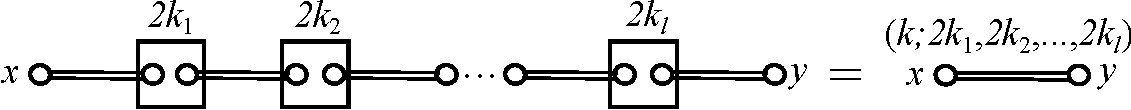
\includegraphics[width=10cm]{Labeldouble.pdf}
\end{center}
\end{definition}
 
 
%\begin{remark}
The scaling order of a labelled $\dashed$ edge is calculated as follows. Taking \eqref{eq label} as an example, there are $l+1$ $\dashed$ edges of total scaling order $2(l+1)$, $\selfs$ $\Sele _{2k_1},\cdots, \Sele_{2k_l}$ of total scaling order \smash{$\sum_{i=1}^l 2 k_i$}, and $2l$ internal atoms of total scaling order $-4l$. Hence the scaling order of \eqref{eq label} is $2(l+1)+\sum_{i=1}^l 2 k_i -4l =k. $ By \eqref{BRB}, \eqref{eq label} is bounded by $W^{-(k-2)d/2+\tau}B_{xy}$ for any constant $\tau>0$, i.e. it has the same decay with respect to $|x-y|$ as $\Theta_{xy}$ except for an extra $W^{-(k-2)d/2}$ factor.  As a convention, both $\dashed$ and labelled $\dashed$ edges will be called ``$\dashed$ edges".
%a $\Theta\Selek_{2l}\Theta$ edge has scaling order $2l$. More precisely, there are two $\dashed$ $\Theta$ edges of scaling order 4, a subgraph $\Selek_{2l}$, and two internal atoms of scaling order $-4$. Hence the total scaling order is $2l$.
%\end{remark}

%We extend the definition of normal regular graphs in Definition \ref{defnlvl0} by including the labelled $\dashed$ edges. Then the definition \eqref{eq_deforderrandom2} of scaling order is extended as 

The scaling order of a normal regular graph with labelled $\dashed$ edges can be equivalently counted as
\begin{align}
  \text{ord}(\cal G) &:= \#\{\text{off-diagonal }  G  \text{ edges}\} + \#\{\text{light weights}\} + 2\#\{ \text{waved edges}\}  + 2 \#\{\text{unlabelled $\dashed$ edges}\} \nonumber\\
&+\sum_k k\cdot   \#\{k\text{-th order labelled $\dashed$ edges}\}  -  2\left[ \#\{\text{internal atoms}\}- \#\{\text{dotted edges}\} \right] . \label{eq_deforderrandom3}
\end{align}
In other words, a $k$-th order labelled $\dashed$ edges is simply counted as an edge of scaling order $k$, and there is no need to count its internal structures using Definition \ref{def scaling}.

%for normal regular graphs with labelled $\dashed$ edges. %This definition is consistent with \eqref{eq_deforderrandom20}.




 
%We introduce the following components to our graphs.
%\begin{itemize}
%
%\item We call a linear combination of $\OO(1)$ many deterministic graphs with the same pair of external atoms and of the same scaling order $k$ a {\bf $k$-th order $\self$} component. For a $k$-th order $\self$ component, say $\Sele_k=((\Sele_k)_{xy}:x,y\in \Z_L^d)$, we use a $\square$ with label $(k,\Sele_k)$ to represent it in the graph. In addition, 
% 
%\item Given $l$ sum zero $\self$ components $\Sele_{2k_i} \in \Cele_{2k_i}$, $1\le i \le l$, as in Definition \ref{collection elements}, we represent the entry
%$ (\Theta \Sele_{2k_1}\Theta  \Sele_{2k_2}\Theta \cdots \Theta  \Sele_{2k_l}\Theta)_{xy}$
% by a labelled $\dashed$ edge between atoms $x$ and $y$ with labels $(k, \Sele_{2k_1}, \cdots , \Sele_{2k_l})$, where $k:=\sum_{i=1}^l 2 k_i -2(l-1)$ is the scaling order of this labelled $\dashed$ edge.  
%We remark that a $\self$ component is used in a labelled $\dashed$ edge only if we know that it satisfies \eqref{two_properties0}-\eqref{weaz}. We also remark that in our graphs, we use labelled $\dashed$ edge as one single edge, and we are not interested in its detailed structure. 
%
%\item Given a normal regular graph $\cal G$ with $\self$ components and labelled $\dashed$ edges, we extend the definition \eqref{eq_deforderrandom2} of scaling order to 
%\begin{align}
% \text{ord}(\cal G)&:= \#\{\text{off-diagonal }  G  \text{ edges}\} + \#\{\text{light weights}\} + 2\#\{ \text{waved edges}\}  + 2 \#\{\text{$\dashed$ edges}\} \nonumber\\
%&+\sum_k k\cdot \left[\#\{k\text{-th order $\self$}\}+ \#\{k\text{-th order labelled $\dashed$ edge}\} \right] \nonumber\\
%& -  2\left[ \#\{\text{internal atoms}\}- \#\{\text{dotted edges}\} \right] . \label{eq_deforderrandom3}
%\end{align}
%\end{itemize}
 
 



%From \eqref{BRB}, we see that $\Theta_{2l}^{(n)}$ has the same behavior as $\Theta$ (except for the extra $W^{-(l-1)d}$ factor). Thus we treat as another type of $\dashed$ edges.
%
%\begin{definition}[Generalized $\Theta$ edges]
%A $\dashed$ edge connecting atoms $x$ and $y$ with label $(n,2l)$ represents a $(\Theta_{2l}^{(n)})_{xy}$ factor. Moreover, the definition \eqref{eq_deforderrandom2} of the scaling/algebraic order can be extended to normal regular  graphs with generalized $\Theta$ edges by treating a $\Theta_{2l}^{(n)}$ as an edge with scaling order $2l$. Finally, the doubly connected property can be extended by 
%including the generalized $\Theta$ edges, where each of them can be either used in the blue net or in the black net. 
%\end{definition}
%
%With \eqref{BRB}, it is easy to see that Lemma \ref{general dot} still holds for the graphs satisfying the extended doubly-connected property with generalized $\Theta$ edges. 



\subsection{Doubly connected property}\label{sec doublenet}

%\iffalse 
%As discussed in Section \ref{sec strategy}, each of our graph has a two-level structure, that is, a local structure on the scale $W$, and a global structure on the scale $L$. To organize the two-level structure, we introduce the following concept of molecules. 
%
%%We first introduce the concept of molecules for the graphs defined in Section \ref{unisec}.
%
%\begin{definition}[Molecules]\label{def_poly}
% We partition the set of all atoms into a union of disjoint sets $\{\text{all atoms}\}=\cup_j \cal M_j$, where each $\cal M_j$ is called a molecule. Two internal atoms belong to the same molecule if and only if they are connected with a path of neutral/plus/minus {\bf waved edges} and {\bf dotted edges} (there may be dotted edges if the graph is not regular). 
%%For the atoms in the same molecules, we always combine them if they are the same (i.e. if they are connected by a dotted line). %Moreover, we assign a dash-dotted line partition of them, that is each two atoms in the same molecule are connected through a cross dah-dotted edge. We do not assign dah-dotted line partitions to all the graph, that is, atoms in different molecules can be the same (except in some middle steps of the expansions, in which case we will mention it explicitly). 
%As a convention, each external atom is called an external molecule (such as $\otimes$, $\oplus$ and $\ominus$ molecules).  %If $\oplus=\ominus$, then we call the molecule containing them as $\oplus$ molecule. 
%An edge is said to be inside a molecule if the ending atoms of this edge both belong to this molecule.
%\end{definition}
%\begin{remark}
%Note that by \eqref{compact f} and \eqref{S+xy}, if two atoms are in the same molecule, then we essentially have $$|x-y|\le (\log W)^2 W$$ up to a negligible error $\OO(W^{-D})$ in all the expressions. 
%\end{remark}
%\fi


Recall the definition of molecules in Definition \ref{def_poly}. We define the molecular graph as the quotient graph of the atomic graph  with the equivalence relation that atoms belonging to the same molecule are equivalent. %Thus we have the following definition.  
%Corresponding to each atomic graph, we can define a molecular graph, whose vertices are molecules.
  
\begin{definition}[Molecular graphs] \label{def moleg}% \cob (need details) \nc 
 Molecular graphs are graphs consisting of 
  \begin{itemize}
\item external molecules which represent the external atoms (such as the $\otimes$, $\oplus$ and $\ominus$ molecules);
\item internal molecules;
\item blue and red solid edges, which represent the plus and minus $G$ edges between molecules;
\item %double-line \hty{ remove double line} 
$\dashed$ edges between molecules;
\item dotted edges between %pairs of \hty{ remove pairs of} 
external and internal molecules.
%  \item dots are molecules
% \item only has blue edges
%\item No inside information of molecule, (\cob we can also leave the local information of blue edges in molecule-level graphs.\nc)  
\end{itemize}
%  \end{definition}
%\begin{definition}  \nc  
Given any atomic graph $\cal G$, we define its molecular quotient graph $ \cal G_{\cal M}$ in the following way:
\begin{itemize}
\item each molecule of $\cal G$ is represented by a vertex in $ \cal G_{\cal M}$;

\item each blue or red solid edge of $\cal G$ between atoms in different molecules is represented by a blue or red solid edge between these two molecules in $ \cal G_{\cal M}$;

\iffalse
\item each solid blue edge inside a molecule becomes a self-loop on this molecule in $ \cal G_{\cal M}$;
\fi

\item each $\dashed$ edge of $\cal G$ between atoms in different molecules is represented by a $\dashed$ edge between these two molecules in $ \cal G_{\cal M}$;

\item each dotted edge of $\cal G$ between an external atom and an internal atom is represented by a dotted edge between the corresponding external and internal molecules;

%\item if there are multiple $\times$-dotted lines between the same pair of molecules, then we only keep one of them; 
%{\it dotted line} between them, which means that there are at least a pair of atoms in these two molecules that always take the same value;

\item we discard all the other components in $\cal G$ (including the weights, $\times$-dotted edges, %red solid $\overline G$ edges, 
and  %waved and $\dashed$ 
all edges inside any molecule). %to $ \cal G_{\cal M}$.
\end{itemize}
 %  \noindent{\bf Simple level 2 standard graphs:} We now introduce a strange trick, that is, we only keep the blue solid edges in the graphs and for the red solid edges we only record the total number of them. More precisely, corresponding to a standard graph $\cal G$, we define the simple standard graph $S(\cal G)$ as the subgraph with only black and grey $\dashed$ edges and blue solid $G$ edges. Note that we will expand the graph $\cal G$ only, and $S(\cal G)$ is used to help to study the molecule family tree structure. (\cor draw an example\nc) 
\end{definition}

We emphasize that molecular graphs are used solely to analyze the graph structures; the expansions in Section \ref{sec_basiclocal}  are only applied to atomic graphs. In the following proof, we assume that each atomic graph is automatically associated with a molecular graph. As discussed below Definition \ref{def_poly}, we call 
%shall call the subgraph inside a molecule (i.e. the subgraph consists of the atoms inside this molecule and the edges between them) a {\it local structure}. On the other hand, we shall call 
the structure of the molecular graph as the {\it global structure} of the atomic graph.  
%Note that the local structures can only vary on scales of order $\OO_\prec(W)$, while the global structure varies on the scale $L$. 

%\hty{ remove the rest in this para} 
%In general, the local structures are almost trivial to bound, while the global structure is much harder to analyze. %This is the main reasons why we want to 
%%By introducing the molecular graphs, we can discard the detailed local structures and focus instead on the .
%This is one of the main reasons why we want to introduce the molecular graphs---we want to get rid of the local structures and focus on the more intricate global structure instead.

%\begin{remark}
%Note that the dotted-line partition of the molecular graph is not necessary consistent. For example, there may be a $G$ edge between two molecules, which is accompanied by a $\times$-dotted line. On the other hand, there may be a dotted edge between the other two atoms in these molecules, and we keep both of them, because, as we said above, the molecule-level-graphs will only be used to help with the analysis.
%\end{remark}
%We now check the orders of the graphs on the RHS of the expansions. First, if $y\ne y'$, then all the graphs in the first two lines on the right-hand side of \eqref{Otheta} are at least one order higher than the original graph. If $y'=y$, then the leading term is  
%\be\label{Othetaleading}m  \Theta_{wy}  \overline G_{yy} f(G),\ee
%which has the same order as the original graph, while the rest of the graphs in the first two lines on the right-hand side of \eqref{Otheta} are at least one order higher than the original graph. 

 
The following \emph{doubly connected} property is a key global property for our proof. It allows us to establish a direct connection between the scaling order of a graph and a bound on its value (cf. Lemma \ref{no dot} below). In fact, all graphs in the $T$-expansion and $\incomp$ will satisfy this property (cf. Definitions \ref{def genuni} and \ref{def incompgenuni}). 

\begin{definition} [Doubly connected property]\label{def 2net}  %\cob details are needed \nc. 
A subgraph $\cal G$ without external molecules is said to be \emph{doubly connected} if its molecular graph $\cal G_{\cal M}$ satisfies the following property. There exist a collection, say $\cal B_{black}$, of $\dashed$ edges and another collection, say $\cal B_{blue}$, of  either blue solid or  $\dashed$ edges  such that (a) $\cal B_{black}\cap \cal B_{blue}=\emptyset$, and (b) both  $\cal B_{black}$ and $\cal B_{blue}$ contain a spanning tree %is a {\bf connected subset of edges}
that connects all molecules in the graph (if there is at most one molecule, this condition holds trivially). For simplicity of notations, we call the $\dashed$ edges in $\cal B_{black}$ as black edges, and the blue solid and $\dashed$ edges in $\cal B_{blue}$ as blue edges. Correspondingly, $\cal B_{black}$ and $\cal B_{blue}$ are referred to as \emph{black net} and \emph{blue net}, respectively,  where a ``net" refers to a subset of edges that contains a spanning tree.  

%On the other hand, given a graph $\cal G$ with external molecules, we say $\cal G$ is doubly connected if the subgraph of $\cal G$ induced on the internal atoms is doubly connected.

A graph  $\cal G$ with external molecules is said to be doubly connected if its subgraph with all external molecules removed is doubly connected, i.e. the spanning trees in the two nets are not required to contain the external molecules.
%(\cor two systems of spanning trees, disconnected\nc)
%We shall call a collection of edges ``a net" if these edges connect all the normal molecules except $\oplus$ and $\otimes$ (i.e. the graph with the normal molecules and the collection of edges is edge connected). We say a graph is a double nets graphs if it has two disjoint nets, where one net consists of black or grey $\dashed$ edges only and the other consists of black dashed, grey dashed or blue solid edges. 
% {\bf Important:} Of course, the 2net concept is correct. But in most calculation/application, the form we used is the one with 1 external black edge and 1 black/blue edge. Therefore, one should introduce a concept i.e., 2net with 2 external edges. The main reason is 
% 1: black external edge will be used in summation 
% 2: blue external edge will be used in expansion. 
% \cob Overall, we need to change from 2net to 2net+2external
\end{definition}




%\begin{remark}
The doubly connected property is defined on molecular graphs, and thus is a \emph{global property}. In the above definition, the $\dashed$ edges also include labelled $\dashed$ edges introduced in Definition \ref{def_graph comp}. The red solid edges are not tracked in the doubly connected property, and the path connectivity of red solid edges can be broken in our expansion procedure in \cite{PartII_high}. By symmetry, we can also define an expansion procedure so that graphs in the $T$-expansion satisfy the doubly connected property with a black net and a red net.   


%In fact, the connectivity of red solid edges will be broken in our expansion procedures. \hty{ remove previous sentence. I am confused with the following remark. }  More precisely, in the graphs from the expansions of the $T$-variables, we generally {\bf do not} have a collection $\cal B_{black}$ of $\dashed$ edges and another disjoint collection $\cal B_{red}$ of red solid and $\dashed$ edges, so that both of them are connected subset of edges that connect all molecules. However, a weaker doubly connected property holds: if we split each $\dashed$ edge into a blue solid edge and a red solid edge, then there is a connected blue net of blue solid edges and a  connected red net of red solid edges in the graph. This property is weaker than the doubly connected property in Definition \ref{def 2net}. 
%{\cor Note that we do not keep the red solid $\overline G$ edges in the molecular graphs. This is because we want to keep the molecular graph as concise as possible, so that we can focus on the structures of the $\dashed$ and plus $G$ edges.} 	
%\end{remark}

%\begin{remark}
%{\cob  Recall that a \emph{one-particle irreducible graph} in Feynman diagrams refers to a graph satisfying the following property: it stays connected if we cut one internal edge in it. From Definition \ref{def 2net}, it is easy to see that a double-net graph is a one-particle irreducible graph on the {\bf molecular level} (it may not be irreducible on the atomic level). On the other hand, the irreducibility may not imply the double-net property of a graph. Hence Definition \ref{def 2net} describes a stronger property of the graphs.}
%\end{remark}

%\begin{remark}
%We have defined the double-net property in a way such that after combining the molecules that are connected through dotted edges, the following property holds. There exist two collections of edges, $\cal B_1$ of black $\dashed$ edges and $\cal B_2$ of blue $\dashed$ and plus $G$ edges, such that $\cal B_1\cap \cal B_2=\emptyset$ and each of them 
% is a subset of edges that connect all the molecules together. Hence there are two distinct connected nets of edges in the graph, which explains the name ``double-net" and ``doubly connected".
%\end{remark}







%\begin{remark}
%Here the two external edges refers to the fact that: there is at least one blue edge between the internal molecules and $\ominus$, and at least one black edge between the internal molecules and $\oplus$. Roughly speaking, the black external edge will be used in summation, and the blue external edge will be used in expansion (if it is a $G$ edge). 
%\end{remark}

%For a doubly-connected graph, we can use its scaling order defined algebraically in \eqref{eq_deforderrandom2} to give an estimate on its graph value as we will show in Lemma \ref{general dot}. This is the main reason why we want to keep the doubly connected property for all the graphs. 

 

 
 \subsection{$T$-expansion with doubly connected structures}
 
For graphs in the $T$-expansion, they are all doubly connected in the sense of Definition \ref{def 2net}. By including this property and the labelled $\dashed$ edges in Definition \ref{def_graph comp}, we are now ready to state the rest of the details for the $T$-expansion in Definition \ref{defn genuni} and the $\incomp$ in Definition \ref{defn incompgenuni}. We will design an expansion strategy in \cite{PartII_high} so that all graphs in the $T$-expansion and $\incomp$ are doubly connected.
%Then it is easy to see that, after removing the external molecules, we still have a doubly connected graph consisting of the internal molecules. 
%But before discussing about the double-net property for the graphs in $T$-expansions, we first need to define a new type of graphical components representing the $\selfs$ in Definition \ref{collection elements}.
%Moreover, for all the graphs appearing in the expansions, there is at least one $\dashed$ edge connecting $\otimes$ to the internal molecules, and at least one blue solid (plus $G$) or $\dashed$ edge connecting $\oplus$ to the internal molecules. 
 
%We now extend Definition \ref{defn genuni} to the $T$-expansions of generalized $T$-variables \eqref{general_T}. Moreover, we will state more detailed properties on the graphs. Even more details will be added later in Definition \ref{def genuni2}. 

%For the definition, we introduce the following two types of graphs. 
%\begin{definition}
%%\begin{itemize}
%
%%\item[(I)] 
%(i) We say a graph is a $\oplus$/$\ominus$-recollision graph, if there is at least one dotted edge connecting $\oplus$/$\ominus$ to an internal atom. 
%
%\medskip
%\noindent(ii) We say a graph is a $Q$-graph if all the $G$ edges and $G$ weights in the graph have the same $Q$ label, i.e. the graph represents a fluctuation term. 
%
%%\item[(III)] deterministic graphs which have no dash-dotted edges connected with $\otimes$, and are deterministic except for the two $|G_{x\otimes}|^2$ edge connected with $\otimes$. 
%%\end{itemize}
%\end{definition}

%We first add more details to Definition \ref{collection elements}. %first describe the collection of labelled $\dashed$ edges.
%\begin{notation}\label{collection labels}
%Let $\Cele_{l}$, $l\in \N$, be the sequence of sets in Definition \ref{collection elements}, that satisfy the following following additional properties. 
%%A sequence of admissible sets of deterministic graphs, denoted by $\Cele_{2l}$ for $l\in \N$, is a family of collections of deterministic graphs $\Selek_{2l}$ such that the following properties hold. 
%\begin{itemize}
%%\item[(i)] For any fixed $l\in \N$, $|\Cele_{2l}|\le C_{l}$ for a large constant depending on $l$. Moreover, we have $\Sdelta_{2l},\Sele_{2l}\in \Cele_{2l}$.
%%\item[(ii)] For each $ \Selek_{2l} \in \Cele_{2l}$, it is a deterministic graph such that $(\Selek_{2l})_{xy}$ is of scaling order $2l$ for any fixed $x$ and $y$.
%\item[(i)] For each $ \Selek_{l} \in \Cele_{l}$, the labelled $\dashed$ edges in it are of the form $ (\Theta \Sele_{2k_1}\Theta  \Sele_{2k_2}\Theta \cdots \Theta  \Sele^{(\kappa_r)}_{2k_r}\Theta)_{xy}$ for $\Sele_{2k_i}\in \cup_{k\le l-1} \Cele_{k}$, $1\le i \le r$.
%\item[(ii)] The graphs $ \Selek_{l} \in \Cele_{l}$ are all doubly connected with labelled $\dashed$ edges as in (i).
%\item[(iii)] Without loss of generality, we assume that $\Sele_{l},\Sele_{l}\in \Cele_{l}$ (recall \eqref{chain S2k} and \eqref{decompose Sdelta})
%%\item[(iii)] Each $ \Selek_{2l} \in \Cele_{2l}$ and its infinite space limit $\Seleinf_{2l}$ satisfy the properties \eqref{two_properties0}-\eqref{weaz}.
%\end{itemize} 
%\end{notation}


%We define the $n$-th order $T$-expansion of generalized $T$-variables as follows. 
\begin{definition} [More properties of the $n$-th order $T$-expansion]
\label{def genuni}
%For any fixed order $n$, suppose we have defined the sequence of deterministic graphs $S^{(k)}_ \Delta$, $2\le k \le n-1$. Then 
An $n$-th order $T$-expansion of $T_{\fa,\fb_1 \fb_2}$ is an expression satisfying Definition \ref{defn genuni} and the following additional properties.

%of the following form: %for any fixed large constant $D>0$,  
%\be\label{mlevelTgdef0}
%T_{\fa,\fb_1 \fb_2}= m  \Theta_{\fa \fb_1}\overline G_{\fb_1\fb_2} +m   \left(\Theta \Sdelta^{(n)}\Theta\right)_{\fa\fb_1} \overline G_{\fb_1\fb_2} + (\PTn)_{\fa,\fb_1 \fb_2} +  (\ATn)_{\fa,\fb_1\fb_2}  + (\QTn)_{\fa,\fb_1\fb_2} .%+ \OO_\prec(W^{-D}).
%\ee
%Furthermore, the graphs on the right-hand side are normal regular graphs (recall Definition \ref{defnlvl0}) and satisfy the following properties with $C_n$ denoting a large constant depending on $n$. Recall that we represent the external atoms by $\otimes\equiv \fa$, $\oplus\equiv \fb_1$, and $\ominus\equiv \fb_2$.

\begin{enumerate}

\item A diffusive edge in the graphs on the right-hand side of \eqref{mlevelTgdef} is either a $\Theta$ edge or a labelled $\dashed$ edge of the form \eqref{eq label} with $4\le 2k_i \le n$. %and $k=\sum_{i=1}^l 2 k_i -2(l-1)\le n-1$. %In other words, the definition of the $n$-th order $T$-expansion only uses lower order $\selfs$. 
%Moreover, the $\dashed$ edges in property (viii) of Definition \ref{defn genuni} can also be labelled $\dashed$ edges.

\item Each graph in $(\PTn)_{\fa,\fb_1\fb_2}$, $(\ATn)_{\fa,\fb_1\fb_2}$, $(\QTn)_{\fa,\fb_1\fb_2}$ and $(\Err_{n,D})_{\fa,\fb_1\fb_2}$ is doubly connected in the sense of Definition \ref{def 2net}. %if all the external atoms $\otimes$, $\oplus$ and $\ominus$ are removed. 
%Together with item (iii), it also implies that each graph of $(\PTn)_{\fa,\fb_1\fb_2}$, $(\ATn)_{\fa,\fb_1\fb_2}$ and $(\QTn)_{\fa,\fb_1\fb_2}$ is doubly connected in the sense of Definition \ref{def 2netex}.

\iffalse
\item There is a sequence of $\selfs$ $\Sele_{l}$, $4\le l \le n-1$, as in Definition \ref{collection elements}, such that the labelled $\dashed$ edges in each graph on the right-hand side of \eqref{mlevelTgdef} can only be of the form \eqref{eq label} with $4\le 2k_i \le n-1$ and scaling order $k:=\sum_{i=1}^l 2 k_i -2(l-1)\le n-1$. Moreover, $\Sdelta^{(n)}$ is a sum of at most $C_n$ many deterministic graphs as in \eqref{decompose Sdelta0}. 
  %In particular, it satisfies the properties \eqref{two_properties0}-\eqref{weaz}. Moreover, each graph in $\Sdelta^{(n)}$ is doubly connected.

\item The graphs on the right hand side depend only on $n$, $m(z)$, $S$, $S^{\pm}(z)$, $\Theta(z)$ and $G(z)$, but do not depend on $W$, $L$ and $d$ explicitly. 

\item $(\PTn)_{\fa,\fb_1\fb_2}$ is a sum of at most $C_n$ many $\oplus/\ominus$-recollision graphs of scaling order $\le n$ and without any $P$ or $Q$ labels.  Moreover, it can be decomposed as 
 \be\label{decomposeP0}(\PTn)_{\fa,\fb_1\fb_2} =\sum_{ k =3}^{ n}(\PTk)_{\fa,\fb_1\fb_2},\ee
 where each $(\PTk)_{\fa,\fb_1\fb_2}$ is a sum of $\oplus/\ominus$-recollision graphs of scaling order $k$. 

\item $(\ATn)_{\fa,\fb_1\fb_2}$ is a sum of at most $C_n$ many graphs of scaling order $> n$ and without any  $P$ or $Q$ labels.  

\item $(\QTn)_{\fa,\fb_1\fb_2} $ is a sum of at most $C_n$ many $Q$-graphs, each of which can be written into the form $\sum_x Q_x(\Gamma_x)$ for some internal atom $x$ and graph $\Gamma_x$ without $P$ or $Q$ labels.  Moreover, we can write 
\be\label{decomposeQ0} (\QTn)_{\fa,\fb_1\fb_2}= \sum_{k=2}^{n} (\QTk)_{\fa,\fb_1\fb_2} + (\cal Q^{(>n)}_T)_{\fa,\fb_1\fb_2},\ee
where each $(\QTk)_{\fa,\fb_1\fb_2}$ is the sum of $Q$-graphs of scaling order $k$, and $(\cal Q^{(>n)}_T)_{\fa,\fb_1\fb_2}$ is the sum of all the $Q$-graphs of scaling order $>n$.

\item In each graph of $(\PTn)_{\fa,\fb_1\fb_2}$, $(\ATn)_{\fa,\fb_1\fb_2}$ and $(\QTn)_{\fa,\fb_1\fb_2} $, we have only one (labelled) $\dashed$ $\Theta$ edge connected with $\otimes$, one plus solid $G$ edge or a $\dashed$ edge connected with $\oplus$, and one minus solid $ G$ edge connected with $\ominus$ if $\ominus \ne \oplus$. Furthermore, there may be some dotted edges connected with $\oplus$ or $\ominus$. 

\item $\Sdelta_k$, $\PTk$ and $\QTk$ do not depend on $n$, i.e. they are the same expressions in every order $T$-expansion.

 %The graphs on the right-hand side of \eqref{mlevelTgdef} satisfy some additional properties, which will be given in Definition \ref{def genuni2}.
\fi
\end{enumerate}

 \end{definition}
   
%Then we define the incomplete $T$-expansions as in Lemma \ref{incomplete Texp}. %but we require that $\Sele_n $ satisfies the sum zero properties \eqref{3rd_property0} and \eqref{weaz}.

 \begin{definition} [More properties of the $n$-th order $\incomp$]\label{def incompgenuni}
 An $n$-th order $\incomp$ of $T_{\fa,\fb_1 \fb_2}$ is an expression satisfying Definition \ref{defn incompgenuni} and the following additional properties.
\begin{enumerate}
	
	%\item $\Sele_n$ is a linear combination of deterministic graphs, which may contain labelled $\dashed$ edges of the form \eqref{eq label}, where we must have that $4\le 2k_i \le n-1$ and $k=\sum_{i=1}^l 2 k_i -2(l-1)\le n-1$.
	
	\item A diffusive edge in $\Sele_n$ and the graphs on the right-hand side of \eqref{mlevelT incomplete} is either a $\Theta$ edge or a labelled $\dashed$ edge of the form \eqref{eq label} with $4\le 2k_i \le n-1$. % and $k=\sum_{i=1}^l 2 k_i -2(l-1)\le n-1$. %{\cor In particular, $(\PITn)_{\fa,\fb_1\fb_2}$, $(\AITn)_{\fa,\fb_1\fb_2}$, $(\QITn)_{\fa,\fb_1\fb_2} $ and $(\Err'_D)_{\fa,\fb_1\fb_2}$ satisfy property (viii) of Definition \ref{defn genuni}, where the $\dashed$ edges can also be labelled $\dashed$ edges.}
	
	
	\item Each graph in $\Sele_n$, $(\PITn)_{\fa,\fb_1\fb_2}$, $(\AITn)_{\fa,\fb_1\fb_2}$, $(\QITn)_{\fa,\fb_1\fb_2}$ and $(\Err'_{n,D})_{\fa,\fb_1\fb_2}$ is doubly connected in the sense of Definition \ref{def 2net}. 
\end{enumerate}

\end{definition}


%\iffalse
% of the following form: %for any fixed large constant $D>0$,  
%\be\label{mlevelTgdef incomp}
%T_{\fa,\fb_1 \fb_2}= m  \Theta_{\fa \fb_1} \overline G_{\fb_1\fb_2} + \sum_x \left(\Theta \wtSdeltan\right)_{\fa x} T_{x,\fb_1\fb_2} + (\PITn)_{\fa,\fb_1 \fb_2} +  (\AITn)_{\fa,\fb_1\fb_2} + (\QITn)_{\fa,\fb_1\fb_2} . %+ \OO_\prec(W^{-D}).
%\ee
%Furthermore, the graphs on the right-hand side are normal regular graphs and satisfy the following properties.
%
%\item The graphs on the right hand side depend only on $n$, $m(z)$, $S$, $S^{\pm}(z)$, $\Theta(z)$ and $G(z)$, but do not depend on $W$, $L$ and $d$ explicitly. 
%
%\item $(\PITn)_{\fa,\fb_1\fb_2}$ is a sum of at most $C_n$ many $\oplus/\ominus$-recollision graphs of scaling order $\le n$ and without any $P$ or $Q$ labels.   Moreover, it can be decomposed as
%\be\label{decomposePIT0}(\PITn)_{\fa,\fb_1\fb_2} =\sum_{ k =3}^{ n}(\PITk)_{\fa,\fb_1\fb_2},\ee
%where each $(\PITk)_{\fa,\fb_1\fb_2}$ is a sum of $\oplus/\ominus$-recollision graphs of scaling order $k$. 
%
%\item $(\AITn)_{\fa,\fb_1\fb_2}$ is a sum of at most $C_n$ many graphs of scaling order $> n$ and without any  $P$ or $Q$ labels.  
%
%\item $(\QITn)_{\fa,\fb_1\fb_2} $ is a sum of at most $C_n$ many $Q$-graphs, and can be written as
%\be\label{decomposeQIT0} (\QITn)_{\fa,\fb_1\fb_2}= \sum_{k=2}^{n} (\QITk)_{\fa,\fb_1\fb_2} + (\cal Q^{(>n)}_{IT})_{\fa,\fb_1\fb_2},\ee
%where each $(\QITk)_{\fa,\fb_1\fb_2}$ is the sum of $Q$-graphs of scaling order $k$, and $(\cal Q^{(>n)}_{IT})_{\fa,\fb_1\fb_2}$ is the sum of all the $Q$-graphs of scaling order $>n$. 
%
%
%\item In each graph of $(\PITn)_{\fa,\fb_1\fb_2}$, $(\AITn)_{\fa,\fb_1\fb_2}$ and $(\QITn)_{\fa,\fb_1\fb_2} $, we have only one (labelled) $\dashed$ $\Theta$ edge connected with $\otimes$, one plus solid $G$ edge or a $\dashed$ edge connected with $\oplus$, and one minus solid $ G$ edge connected with $\ominus$ if $\ominus \ne \oplus$. Furthermore, there may be some dotted edges connected with $\oplus$ or $\ominus$. 
%
%%we have at least a $\dashed$ $\Theta$ edge connected with $\otimes$, at least a plus solid $G$ edge or a $\dashed$ edge or a dotted edge connected with $\oplus$, and at least a minus solid $G$ edge or a dotted edge connected with $\ominus$.
%
%%There is a sequence of $\selfs$ $\Sele_{l}$, $4\le l \le n-1$, as in Definition \ref{collection elements}, such that the labelled $\dashed$ edges in each graph on the right-hand side of \eqref{mlevelTgdef} can only be of the form \eqref{eq label} with $4\le 2k_i \le n-1$ and scaling order $k:=\sum_{i=1}^l 2 k_i -2(l-1)\le n-1$. Moreover, $\Sdelta^{(n)}$ is a sum of at most $C_n$ many deterministic graphs as in \eqref{decompose Sdelta0}. 
%%In particular, it satisfies the properties \eqref{two_properties0}-\eqref{weaz}. Moreover, each graph in $\Sdelta^{(n)}$ is doubly connected.
%
%\item $\wtSdeltak$, $\PITk$ and $\QITk$ do not depend on $n$, i.e. they are the same expressions in every order $\incomp$.
%
%\item There is a sequence of $\selfs$ $\Sele_{l}$, $4\le l \le n-1$, as in Definition \ref{collection elements}, such that the labelled $\dashed$ edges in each graph on the right-hand side of \eqref{mlevelTgdef incomp} can only be of the form \eqref{eq label} with $4\le 2k_i \le n-1$ and scaling order $k:=\sum_{i=1}^l 2 k_i -2(l-1)\le n-1$. Moreover, $\wtSdeltan$ can be written as \eqref{decompose Sdelta}, where $\Sele_n$ satisfies the properties \eqref{two_properties0}, \eqref{4th_property0}, \eqref{two_properties0V}, \eqref{3rd_property0 diff} and \eqref{4th_property0V} with $l=n$. {\cor add double-net properties of $\Sele_n$}
%
%
%
%% if all the external atoms $\otimes$, $\oplus$ and $\ominus$ are removed.  %Together with item (iii), it also implies that each graph of $(\PITn)_{\fa,\fb_1\fb_2}$, $(\AITn)_{\fa,\fb_1\fb_2}$ and $\QITn_{\fa,\fb_1\fb_2}$ is doubly connected in the sense of Definition \ref{def 2netex}.
%%\item $\wtSdeltan$ can be decomposed as in \eqref{decompose Sdelta}, where each $\Sele_{l}$, $4\le l \le n$, satisfies the properties \eqref{two_properties incomp}-\eqref{4th_propertyV incomp}. Moreover, each $\Sele_{l}$, $4\le l \le n-1$, satisfies \eqref{3rd_property0} and \eqref{weaz}. % and the labelled $\dashed$ $\Theta$ edges in each graph of $\Sele_{2l}$ can only be of the form $\Theta \Sdelta_{2k}\Theta$ or $\Theta \wtSdelta_{2k}\Theta$ with $k<l$.
%%The graphs on the right-hand side of \eqref{mlevelTgdef} satisfy more properties, which will be given later in Definition \ref{def genuni2}.
%
%
%The graphs on the right-hand side of \eqref{mlevelTgdef incomp} satisfy some additional properties, which will be given in Definition \ref{def genuni2}.
%\fi




%In Sections \ref{sec_basiclocal} and \ref{sec global}, we will describe how to construct the $n$-th order incomplete $T$-expansion and the $n$-th order $T$-expansion. In other words, we shall prove Lemma \ref{incomplete Texp} and Lemma \ref{lem completeTexp} there. Before that, we first prove some important estimates on doubly connected graphs. These estimates will imply Lemma \ref{lem V-R wt} and Lemma \ref{lem informal}.

%\section{Analysis of graphs}\label{sec Sdelta}


\subsection{Bounding doubly connected graphs}\label{sec bound double}



In this subsection, we give some important estimates on doubly connected graphs in Lemma \ref{no dot}. In particular, these estimates will be used crucially in the proofs of Lemma \ref{lem V-R wt} and Lemma \ref{lem informal}, and in the proof of Lemma \ref{lemma ptree} in \cite{PartII_high}. We introduce the following weak and strong norms, which control the maximum and the local averages of the entries of a matrix (weak norms) or the decay of its entries (strong norms), and which will be a convenient tool for the proof of Lemma \ref{no dot}. %in bounding graphs with complicated structures.

\begin{definition}\label{Def PseudoG} 
Given a $\Z_L^d\times \Z_L^d$ matrix $\cal A$ and some fixed $a,b>0$, we define its weak-$(a,b)$ norm as
$$\|\cal A\|_{w;(a,b)}:= W^{a d/2}\max_{x,y\in \Z_L^d} \left|\cal A_{xy}\right| + \sup_{ K \in [W, L/2]} \left( \frac{W}{K}\right)^b K^{ad/2} \max_{x, x_0\in \Z_L^d} \frac1{K^d}\sum_{y:| y - x_0 |\le K} \left(\left|\cal A_{xy}\right|+\left| \cal A_{yx}\right| \right),$$
and its strong-$(a,b)$ norm as
$$\|\cal A\|_{s;(a,b)}:= \max_{x,y\in \Z_L^d} \left( \frac{W}{\langle x-y\rangle}\right)^b \langle x-y\rangle^{ad/2} \left|\cal A_{xy}\right|.$$
\end{definition}

%\hty{ what about define 
%
%\newcommand{\normt}[1]{ \| \!  | {#1} \| \!  |}
%
%
%\be
%\normt{\cal A}_{p; a,b}:= W^{a d/2}\max_{x,y\in \Z_L^d} \left|\cal A_{xy}\right| + 
%\sup_{ K \in [W, L/2]}  \left( \frac{W}{K}\right)^b K^{(a-2)d/2}   \Big [ \max_{x, x_0\in \Z_L^d} \sum_{y:| y - x_0 |\le K} \left(\left|\cal A_{xy}\right|+\left| \cal A_{yx}\right| \right)^p \Big ]^{1/p} 
%\ee
%
%Then the weak norm is the $L_1$ and strong is the $L_\infty$?  You can also fix the triple norm and find a good macro. 
%
%} 


%We will use frequently the following facts: if $\|\cal A\|_{w;(a,b)}\prec 1$, then 
%\be\label{eq PseudoG2} 
%\max_{x,y\in \Z_L^d} \left|\cal A_{xy}\right| \prec W^{-a d/2},
%\ee
%and for all $  K \in [W, L/2]$, 
%\be\label{eq PseudoG}
%\max_{x, x_0\in \Z_L^d} \frac1{ K^{d}}\sum_{y:| y - x_0 |\le K} \left(\left|\cal A_{xy}\right|+\left| \cal A_{yx}\right| \right)\prec \left( \frac{K}{W}\right)^b \left(\frac{1}{K^{d/2}}\right)^a;
%\ee
%if $\|\cal A\|_{s;(a,b)}\prec 1$, then 
%\be\label{eq unifG}
%\left|\cal A_{xy}\right| \prec \left( \frac{\langle x-y\rangle}{W}\right)^b \left(\frac{1}{\langle x-y\rangle^{d/2}}\right)^a.
%\ee
%%\begin{definition}[Weak norm and strong norm]\label{Def PseudoG}
%%	Given a $\Z_L^d\times \Z_L^d$ matrix $\cal A$ and some fixed $a,b>0$, we say that $\cal A$ (or the variable $\cal A_{xy}$) satisfies the {\bf level-$(a,b)$ averaged bound}, %or $\cal A_{xy}$ is a variable satisfying the {\bf level-$(a,b)$ averaged bound}, 
%%	if the following properties hold: 
%%	\be\label{eq PseudoG2} 
%%	\max_{x,y\in \Z_L^d} \left|\cal A_{xy}\right| \prec W^{-a d/2},
%%	\ee
%%	and for all $  K \in [W, L/2]$, 
%%	\be\label{eq PseudoG}
%%	\max_{x, x_0\in \Z_L^d} \frac1{ K^{d}}\sum_{y:| y - x_0 |\le K} \left(\left|\cal A_{xy}\right|+\left| \cal A_{yx}\right| \right)\prec \left( \frac{K}{W}\right)^b \left(\frac{1}{K^{d/2}}\right)^a.
%%	\ee
%%	On the other hand, we say that $\cal A$ (or the variable $\cal A_{xy}$) satisfies the {\bf level-$(a,b)$ pointwise bound} if the following estimate holds uniformly in $x,y \in \Z_L^d$:
%%	\be\label{eq unifG}
%%	\left|\cal A_{xy}\right| \prec \left( \frac{\langle x-y\rangle}{W}\right)^b \left(\frac{1}{\langle x-y\rangle^{d/2}}\right)^a.
%%	\ee
%%\end{definition}
%%\begin{remark}
%The strong-$(a,b)$ norm is strictly stronger than the weak-$(a,b)$ norm if $ad/2-b \le d$ (in this paper, we only consider the cases with $a\le 2$). 


In this paper, we only use weak or strong-$(a,b)$ norms with $0\le ad/2-b<d$. In this case, it is not hard to check that the weak-$(a,b)$ norm is bounded by a constant times the strong-$(a,b)$ norm, i.e., the strong-$(a,b)$ norm is stronger than the weak-$(a,b)$ norm. By Definition \ref{Def PseudoG}, we immediately get the bounds
\be\label{eq PseudoG2} 
\max_{x,y\in \Z_L^d} \left|\cal A_{xy}\right| \le W^{-a d/2}\|\cal A\|_{w;(a,b)},
\ee
\be\label{eq PseudoG}
\max_{x, x_0\in \Z_L^d} \frac1{ K^{d}}\sum_{y:| y - x_0 |\le K} \left(\left|\cal A_{xy}\right|+\left| \cal A_{yx}\right| \right)\le   \frac{1}{W^b K^{ad/2-b}}  \|\cal A\|_{w;(a,b)},\quad \text{for all $  K \in [W, L/2]$,}
\ee
\be\label{eq unifG}
\left|\cal A_{xy}\right| \le    \frac{1}{W^b \langle x-y\rangle^{ad/2-b}} \|\cal A\|_{s;(a,b)}.
\ee
Here we list the weak or strong norms of some key deterministic or random variables. 
\begin{enumerate}
\item %$B_{xy}$ satisfies the {level-$(2,2)$ pointwise bound}, and $B_{xy}^{1/2}$ satisfies the {level-$(1,1)$ pointwise bound}. 
$\|B\|_{s;(2,2)}\le 1$ and $\|B^{(1/2)}\|_{s;(1,1)}\le 1$, where $B^{(1/2)}$ is the matrix with entries $(B_{xy})^{1/2}$; % has strong-$(1,1)$ norm bounded by $\OO_\prec(1)$. %satisfies the {level-$(2,2)$ pointwise bound}, and $B_{xy}^{1/2}$ satisfies the {level-$(1,1)$ pointwise bound}. 

\item If \eqref{locallaw1} holds, then $\|G(z)-m(z)I_N\|_{s;(1,1)}\prec 1$. % satisfies the level-$(1,1)$ pointwise bound.  

\item If a matrix $\cal A$ satisfies $|\cal A_{xy}|\le B_{xy}^{1/2}$ for all $x,y\in \Z_L^d$, then $\|\cal A\|_{w;(1,2)}\le C$ for a constant $C>0$ depending only on $d$. In particular, on the event $\{Y(z)\le W^{\e_1}\}$ (recall \eqref{def XY}), we have $\|G(z)-m(z)I_N\|_{w;(1,2)}\le CW^{\e_1}$.

%$W^{-\e_0}|G_{xy}(z)-m(z)\delta_{xy}|$ satisfies the level-$(1,2)$ averaged bound, and $W^{-2\e_0}T_{xy}(z)$ satisfies the level-$(2,4)$ averaged bound. %Furthermore, by Lemma \ref{lem G<T},.  

%and $W^{-\e_0}T_{xy}^{1/2}(z)$ are pseudo $G$ variables. 

\item The following positive random variable $\Psi_{xy}$ was defined in \cite[Definition 3.4]{PartIII} for a small constant $\tau>0$ and a large constant $D>0$:
\be\label{eq defPsi}
\Psi^2_{xy}\equiv \Psi^2_{xy}(\tau,D) :=W^{-D}+ \max\limits_{ \substack{|x_1-x| \le   W^{1+\tau}  \\ |y_1-y|\le  W^{1+\tau}}}s_{x_1y_1} + W^{-(2+2\tau)d}\sum_{ |x_1-x| \le  W^{1+\tau}}\sum_{ |y_1-y|\le  W^{1+\tau}} |G_{x_1y_1}|^2  .\ee
Note that  $\|\Psi(z)\|_{w;(1,2)} \prec \|G(z)-m(z)I_N\|_{w;(1,2)} + 1$ and  $\|\Psi(z)\|_{s;(1,1)} \prec \|G(z)-m(z)I_N\|_{s;(1,1)} + 1$ as long as $D$ is large enough.

%If \eqref{Gmax} and \eqref{initial Txy222} hold, then $\|\Psi(z)\|_{w;(1,2)} \prec W^{\e_0}$. % satisfies the level-$(1,2)$ averaged bound. 
\end{enumerate}
The motivation for introducing the $\Psi$ matrix is as follows: given $x_1,x_2\in \Z_L^d$, suppose $y_1$ and $y_2$ satisfy that  
\be\label{y12x12}|y_1-x_1|\le W^{1+\tau/2} ,\quad |y_2-x_2|\le W^{1+\tau/2}.\ee 
If $y_1\ne y_2$ and we know that $\|G(z)\|_{\max}\prec 1$, then using Lemma \ref{lem G<T} we can obtain the bound 
\begin{align}
|G_{y_1y_2}(z)|^2&\prec T_{y_1y_2}(z) =|m|^2 s_{y_1y_2}|G_{y_2y_2}(z)|^2 +|m|^2 \sum_{\al\ne y_2}s_{y_1 \al}|G_{\al y_2}(z)|^2 \nonumber\\
&=|m|^2 s_{y_1y_2}|G_{y_2y_2}(z)|^2 +|m|^2 \sum_{\al\ne y_2}s_{y_1 \al}|G_{y_2\al }(\overline z)|^2 \nonumber\\
&\prec   s_{y_1y_2} +  \sum_{\al\ne y_2}s_{y_1\al} T_{ y_2 \al}(\overline z)  \le s_{y_1y_2} + \sum_{\al ,\beta} s_{y_1\al}s_{y_2\beta} |G_{\al\beta }(z)|^2 \nonumber\\
&\le W^{-D}+s_{y_1y_2} + W^{-2d}\sum_{|\al-y_1|\le W^{1+\tau/2}}\sum_{|\beta-y_2|\le W^{1+\tau/2}}  |G_{\al\beta}(z)|^2  \le W^{2d\tau} \Psi_{x_1x_2}^2(\tau,D),\label{Gpsi}
\end{align}
%as long as we have  and $C_\psi>2$. Here 
where in the third and fifth steps we used the simple identity $G_{xy}(z)=\overline{G_{yx}(\overline z)}$, in the fourth step we used \eqref{offG largedev} with $z$ replaced by $\overline z$, i.e., its column form $\mathbf 1_{\al\ne y_2}|G_{\al y_2}(z)|^2\prec |m|^2\sum_{\beta}s_{y_2\beta}|G_{\al\beta}(z)|^2$, which holds under the same assumptions, and in the sixth step we used \eqref{subpoly}. In particular, if $y_1$ and $y_2$ are in the same molecules as $x_1$ and $x_2$, respectively, then we know that \eqref{y12x12} holds, since otherwise the graph value will be smaller than $W^{-D}$ for any fixed $D>0$ by \eqref{subpoly} and \eqref{S+xy}. Then \eqref{Gpsi} shows that all the $G$ edges between two molecules containing atoms $x_1$ and $x_2$ can be bounded with the same variable $\Psi_{x_1x_2}$. This fact will be convenient for our proof. % and will be used in the proof of Lemma \ref{no dot}.
%\end{remark}

%
%Then we have a similar estimate as in \eqref{BG14} for pseudo $G$ variables. 
%\begin{lemma}
%Let $\cal A$ be a pseudo resolvent as in Definition \ref{Def PseudoG}. Under the assumption of Lemma \ref{lem: ini bound}, for $d\ge 14$ we have that 
%\be\label{BGpseudo}
%\max_{y,z} \sum_{ x }B_{xy}\cal A_{xz} \prec   W^{-d/2+\e_0}.
% \ee
% %if $\eta/\wt\eta \ge W^{-\e_0}$ for some sufficiently small constant $\e_0>0$.
% \end{lemma}
% \begin{proof}
% The proof is the same as the one for Corollary \ref{cor: ini bound} using the two properties \eqref{eq PseudoG} and \eqref{eq PseudoG2}.
% \end{proof}
 

By \eqref{sumTheta}, the row sums of $\Theta$ diverge when $L\to \infty$ (e.g. if $\eta=W^{2}/L^{2-\e}$). On the other hand, the following claim shows that the product of a $\Theta$ entry and a variable with bounded weak-$(1,2)$ norm is summable if $d\ge 8$. Although this claim will not be used in our proof directly, it explains why we require $d\ge 8$ in Theorem \ref{main thm0}. Our proof of Lemma \ref{no dot} is actually based on some more general versions of this claim in \eqref{keyobs3} and \eqref{keyobs2} below.

%{\cor talk about the dimension $d\ge 7$} With the continuity estimate \eqref{initial Txy2}, we show that a $\Theta$ edge together with a long $G$ edge essentially provide a $W^{-d/2}$ factor when $d\ge 14$.
 
 \begin{claim}\label{cor: ini bound} 
 %Suppose $G(z)$ satisfies \eqref{initial Txy2}. 
Let $\cal A$ be a matrix satisfying $\|\cal A\|_{w;(a,b)}\prec 1$ % level-$(a,b)$ averaged bound 
for some fixed $a,b>0$. If 
 \be\label{a+b}
 a d/2 - b - 2\ge 0,
 \ee
then we have that
 %Under the assumption of Lemma \ref{lem: ini bound}, for $d\ge 14$ we have that 
\be\label{BG14}
\max_{x,y\in \Z_L^d} \sum_{ \al }B_{x\al}\cal A_{y\al} \prec  W^{-a d/2}.
 \ee
% if $\eta/\wt\eta \ge W^{-\e_0}$ for some sufficiently small constant $\e_0>0$.
  \end{claim}
  
  \begin{proof}
% In \cite{PartIII}, we have proved the following $T$-equation estimate
%\be\label{Tweak} 
%T_{xy} \prec B_{xy} + \Phi^2 \Gamma^2,
%\ee
%where $\Phi$ and $\Gamma$ are deterministic parameters such that
%$$  \|T\|_{\max} \prec \Phi^2, \quad \max_{\fa,\fb}\sum_{x}B_{\fa x} T_{x \fb}\prec \Gamma^2.$$
%We assume that
%\be\label{initial Txy3}T_{xy}\prec B_{xy} + \wt\Phi^2 .\ee
%We now see how we can improve the estimates on $\wt\Phi$.
%
%Without loss of generality, we assume $\eta/\wt\eta = W^{-\e_0}$. For $\sum_{x}B_{\fa x} T_{x \fb}$, we decompose the sum according to the dyadic scales: $x\in \cal I_{n,m}:=\{x\in \Z_L^d: K_{n-1} \le |\fa-x| \le K_{n},K_{m-1} \le |x-\fb| \le K_{m}\}$, where $K_n:= 2^n W$ for $1\le n \le \log_2 (L/W) +1$ and $K_{0}:=0$. Then using \eqref{initial Txy2} and the fact that $I_{n,m}$ is inside a box of scale $K_{n}\wedge K_{m}$, we can estimate that 
%\begin{align*}
%\sum_{x\in \cal I_{n,m}}B_{\fa x} T_{x \fb} &\prec \left( \frac{\wt\eta}{\eta}\right)^2 \frac{W^{-1}\left( K_n\wedge K_m\right)^{d/2+1}}{W^2 K_{n}^{d-2}} \lesssim \left( {\wt\eta}/{\eta}\right)^2W^{-d/2}.
%\end{align*}
%Since there are at most $\OO( (\log L)^2)$ many such sets $\cal I_{n,m}$, we obtain that 
%%First using \eqref{initial Txy2} and a dyadic decomposition argument, we obtain that
%$$\Gamma^2 \prec \left( {\wt\eta}/{\eta}\right)^2W^{-d/2}= W^{-d/2+2\e_0} \ \Rightarrow \ T_{xy}\prec B_{xy} + W^{-d/2+2\e_0}\Phi^2.$$
%This gives a self-improving estimate for $\Phi$, and after $\OO(1)$ many inductions we get $\Phi \prec W^{-d/2} $, which by Lemma \ref{lem G<T} gives
%%Note that one immediate consequence of this estimate is the $l^\infty$ bound ({\cob add a reference}), 
%\be\label{Gmax} \|G(z)-m(z)\|_{\max}\prec W^{-d/2}. \ee
%%This is optimal if we only use the old $T$-equation estimate.  
%Then with \eqref{Tweak} we get
%$$T_{xy} \prec B_{xy} + W^{-d} \Gamma^2 \ \Rightarrow \  T_{xy}\prec B_{xy} + W^{-3d/2+2\e_0}.$$
%We now bound $\Gamma^2$ using \eqref{initial Txy3}. For simplicity, we introduce the short-hand notation $b_K:= W^{-2}K^{-d+2}$. For scale $K$ such that $b_K^{1/2} \ge \wt\Phi^2$, we bound
%$$\sum_{y \in \cal I_K} B_{xy} T_{yw} \prec \frac{1}{W^4K^{d-4}}+ {\wt\Phi^2}\frac{K^2}{W^2}, \quad \cal I_K:=\{ y: K\le |y-x|\le 2K\},$$
%where we applied \eqref{Tweak} to $T_{yw}$. Otherwise, using \eqref{initial Txy2}  we can bound that
%$$\sum_{y \in \cal I_K} B_{xy} T_{yw} \prec \frac{W^{2\e_0}}{W^3K^{d/2-3}}.$$
% Thus summing over all scales and maximizing over $K$, we get that
%$$\Gamma^2 \prec  W^{-d} + W^{-\frac{2d}{d-2} + \frac{8\e_0}{d-2}} \wt\Phi^{\frac{2d-12}{d-2}}.$$
%Hence we get the $T$-equation estimate
%$$ T_{xy}\prec B_{xy} + W^{-2d} + W^{-\frac{d^2}{d-2}+ \frac{8\e_0}{d-2}} \wt\Phi^{\frac{2d-12}{d-2}}  \prec  B_{xy} + W^{-2d} + W^{\e}W^{-\frac{d^2}{4}+ 2\e_0} + W^{-\e}\wt\Phi^2  ,$$
%for any fixed $\e>0$. This gives a self-improving estimate for $\wt\Phi$, and iterating this estimate we get
%\be\label{offT} T_{xy}\prec B_{xy} + W^{-2d}. \ee %\wt\Phi^2, \quad \wt\Phi^2 = W^{-\frac{d^2}{4}}   .$$
We decompose the sum over $\al$ according to the dyadic scales: 
$$\al\in \cal I_{n,m}:=\{\al\in \Z_L^d: K_{n-1} \le |x-\al| \le K_{n},K_{m-1} \le |y-\al| \le K_{m}\},$$ 
where $K_n$ are defined in \eqref{defn Kn}. Then using \eqref{eq PseudoG} and the fact that $\cal I_{n,m}$ is inside a box of scale $\OO(K_{n}\wedge K_{m})$, we can estimate that %for $n,m\ge 1$,
\begin{align*}
\sum_{\al\in \cal I_{n,m}}B_{x\al} \cal A_{y\al} &\prec \frac{1}{W^2K_n^{d-2}}\sum_{\al\in \cal I_{n,m}}\cal A_{y\al}  \prec   \frac1{W^{2} K_{n}^{d-2} }\cdot \frac{\left( K_n\wedge K_m\right)^{d}}{ W^b(K_n\wedge K_m)^{ad/2-b}}  \\
&\le  \frac{1}{ W^{b+2}(K_n\wedge K_m)^{ad/2-b-2}}  \le  W^{-a d/2},
\end{align*}
where in the last step we used \eqref{a+b}. Summing over $\OO( (\log L)^2)$ many such sets $\cal I_{n,m}$, we get that 
$$\sum_{ \al }B_{x\al} \cal A_{y\al} \prec (\log L)^2  W^{-a d/2}\prec W^{-a d/2}.$$
This concludes the proof.
%First using \eqref{initial Txy2} and a dyadic decomposition argument, we obtain that
%Finally we bound $\sum_{y}B_{xy}|G_{yw}|$ using the initial estimates. With similar arguments as above, we can bound
%\be\label{initial0}
%\sum_{y \in \cal I_K} B_{xy} T^{1/2}_{yw} \prec \frac{1}{W^{d/2}}+\min\left\{ {\wt\Phi}\frac{K^2}{W^2}, \frac{W^{\e_0}}{W^{\frac52}K^{\frac{d}{4}-\frac52}}\right\}.
%\ee
%In particular, we see that the second term is maximized when $W^{-d}=\wt\Phi = W^{-1/2+\e_0}K^{-d/4+1/2}.$ Solving $K$ and plugging it into the above bound, we obtain that
%\be\label{initial01}
%\sum_{y \in \cal I_K} B_{xy} T^{1/2}_{yw} \prec \frac{1}{W^{d/2}} + \frac{W^{\frac{8\e_0}{d-2}}}{W^{\frac{d(d-8)}{d-2}}} .\ee%+ \frac{1}{W^{\frac52 + \frac{(2d-1)(d-10)}{2(d-2)} } }.$$
%Thus for $d\ge 14$, it produces a $W^{-d/2}$ factor (up to a $W^{\e_0}$ factor). %; otherwise, for $10\le d < 14$, it produces a $ W^{-d/4}$ factor (up to a $W^{\e_0}$ factor).
\end{proof}


%\begin{remark}
If $\|G(z)-m(z)I_N\|_{w;(1,2)}\prec 1$, % satisfies the level-$(1,2)$ averaged bound, 
then by Claim \ref{cor: ini bound} we have that
$$\max_{x,y\in \Z_L^d} \sum_{ \al }B_{x\al}|G_{y\al}| \prec  W^{- d/2} $$
if $d/2-4\ge 0$, which gives $d\ge 8$. 
%If $d\ge 6$, we can further bound \eqref{bound 2net1B} as
%\be\label{d>7} \left| \cal G_{0} (x,y) \right|\le W^{-(n_{xy}/2-2)d}\frac{W^{\e}}{W^4\langle x-y\rangle^{2d-4}} \le W^{-(n_{xy}/2-1)d}\frac{W^{2+\e}}{\langle x-y\rangle^{d+2}},\ee
%which explains the property \eqref{4th_property incomp}. 
%where we used $d\ge 7$ in the last step. This concludes \eqref{Sdelta double}. For \eqref{d>7} to hold, we only need $d\ge 6$. 
\iffalse
If we can improve the continuity estimate \eqref{initial Txy2} to 
 \be\nonumber
K^{-d} \max_w\sum_{|y-w|\le K} \left(|G_{xy}( z)|^2 + |G_{yx}( z)|^2\right) \prec \left(\frac{\wt \eta} {\eta}\right)^2 \frac{1}{W^3K^{d-3}},
\ee
then $\frac{\eta}{\wt\eta}|G_{xy}(z)-m(z)\delta_{xy}|$ satisfies the level-$(1,3/2)$ averaged bound and \eqref{a+b} gives $d\ge 7$. In this case, all the arguments in this paper still hold and we can conclude Theorem \ref{comp_delocal} and Theorem \ref{main thm0} for $d=7$. %This case is still under study. %We have done this because we would like to make sure the above arguments also work for the $d\ge 6$ case, which 
%This will be a topic for future study. 
A much more challenging task is to show that $\frac{\eta}{\wt\eta}|G_{xy}(z)-m(z)\delta_{xy}|$ actually satisfies the (almost sharp) level-$(1,1)$ averaged bound, in which case we can conclude Theorem \ref{comp_delocal} and Theorem \ref{main thm0} for $d=6$. Finally, for $d\le 5$, the proof of this paper fails, and new tools have to be developed. \fi
%\end{remark}
We now prove the following key estimates on doubly connected graphs. %satisfying Definition \ref{def 2net}. 
 
\begin{lemma}\label{no dot}
%(\copu assume there are some estimates on $T$\nc) 
 Suppose $d\ge 8$ and $\cal G$ is a doubly connected normal regular graph without external atoms, whose diffusive edges are $\Theta$ edges or labelled $\dashed$ edges of the form \eqref{eq label}, and whose solid edges and weights are evaluated with an $N\times N$ matrix $G$ (which may be $G(z)$ or any other matrix). % that $|G_{xy}(z)-m(z)\delta_{xy}|$ satisfies the level-$(1,2)$ averaged bound. \eqref{initial Txy222} and \eqref{Gmax} hold, $d\ge 7$, $\eta\ge W^{2+\e}/L^2$ and $\eta/\wt\eta\ge W^{-\e_0}$ for some small constants $\e,\e_0>0$.
Let $\Lambda$ be a parameter satisfying $1\le \Lambda\le W^{d/2}$ and $\|G-m(z)I_N\|_{w;(1,2)}\le \Lambda$. % defined in Definition \ref{def 2net}.
%off-$G$-property (recall Definition \ref{defnlvl0}) and the doubly connected property. Let $\cal G_0$ be the subgraph consisting of the internal molecules only, and suppose that $\cal G_0$ is also doubly connected.
Pick any two atoms of $\cal G$ (which may belong to the same molecule) and fix their values $x , y\in \Z_L^d$. Then the resulting graph $\cal G_{xy}$ satisfies  that %that
%\be\label{bound 2net1}
%\|\wh{\cal G}\|_{w;(1,2)}\prec 1, \quad \text{with} \ \ \wh {\cal G}_{xy}:=  W^{\left(n_{xy}-3\right)d/2 } \cal G_{xy}/ B_{xy} ,
%\ee
\be\label{bound 2net1}
\left|\cal G_{xy}\right| \prec W^{ - \left(n_{xy}-3\right)d/2 } B_{xy} \cal A_{xy}\cdot \Lambda^{n_{xy}-2},
\ee
where  $n_{xy}:=\ord(\cal G_{xy})$ is the scaling order of $\cal G_{xy}$ and  $\cal A_{xy}$ is some  positive variable  satisfying $\|\cal A\|_{w;(1,2)}\prec 1$.
%$n_{xy}:=\ord((\cal G_0)_{xy})$,
%and $\cal A_{xy}$ is a positive variable satisfying the level-$(1,2)$ averaged bound.
Furthermore, %if $|G_{xy}(z)-m(z)\delta_{xy}|$ satisfies the stronger level-$(1,1)$ pointwise bound,
if $\|G-m(z)I_N\|_{s;(1,1)}\le \Lambda$ instead, then we have that
\be\label{bound 2net1 strong}
\left|\cal G_{xy}\right| \prec W^{ -  \left(n_{xy}-3\right)d/2} B_{xy}^{3/2}\cdot \Lambda^{n_{xy}-2}.
\ee
If we fix an atom $x \in \cal G$, then  the resulting graph  $\cal G_{x}$ satisfies  that
\be\label{bound 2net1 singlex}
\left|\cal G_{x}\right| \prec W^{ - \ord(\cal G_{x}) \cdot d/2 }\cdot \Lambda^{\ord(\cal G_{x})} .
\ee
Here $\prec$ is understood in the sense of Definition \ref{stoch_domination} (ii), uniformly in $G$ and $\Lambda$ satisfying the above assumptions. The above bounds  hold also  for the graph $ {\cal G}^{{\rm abs}}$, which is obtained by replacing each component (including edges, weights and coefficients) in $\cal G$ with its absolute value and ignoring all the $P$ or $Q$ labels (if any). We emphasize that in defining $ {\cal G}^{{\rm abs}}$, a labelled $\dashed$ edge \eqref{eq label} will be regarded as one single edge and replaced by $|\left(\Theta \Sele_{2k_1}\Theta  \Sele_{2k_2}\Theta \cdots \Theta  \Sele_{2k_l}\Theta\right)_{xy}|$.
%satisfying the following estimates: 
% \be \label{bound 2netAA}
%\max_{x,y}\cal A_{xy}\prec W^{-d/2},\quad K^{-d} \max_w\sum_{|y-w|\le K} \cal A_{xy}( z)\prec   \frac{1}{W^{1/2}K^{d/4-1/2}},\quad  z=E+ \ii\eta,
%\ee
%for any $W\le K \le L$.
% where the order is defined in \eqref{eq_deforderrandom2}.
% where $A$ is   2net connected, and contains $ \al$, $\beta  $.  
 \end{lemma}

% The graph $\cal G_{xy}$ in this lemma can be regarded as a doubly connected graph where the black and blue nets also contain the external atoms $x$ and $y$. The estimate \eqref{bound 2net1} can be stated in a form that is easier to understand: $\left|\cal G_{xy}\right| \prec W^{ - \left(n_{xy}-3\right)d/2 } B_{xy} \cal A_{xy},$ for a positive variable $\cal A_{xy}$ satisfying $\|\cal A\|_{w;(1,2)}\prec 1$. In the following proof, we will state such estimates in this way. 
%%``$ {\left|\cal G_{xy}\right| }W^{\left(n_{xy}-3\right) d/2}/ B_{xy} $ is a random variable  satisfying the level-$(1,2)$ averaged bound", but the form \eqref{bound 2net1} is clearer in its meaning. 
%
%\hty{ we now can remove previous comment and just keep the rest} 

Note that a doubly connected graph $\cal G$ with at least two molecules must have $n_{xy}\ge 3$.  If $x$ and $y$ are in the same molecule, then \eqref{bound 2net1} gives the sharp bound $\left|\cal G_{xy}\right| \prec W^{ - n_{xy} d/2 }\Lambda^{n_{xy}-2}$. If $\|G(z)-m(z)I_N\|_{w;(1,2)}\prec 1$ (resp. $\|G(z)-m(z)I_N\|_{s;(1,1)}\prec 1$), then applying \eqref{bound 2net1} (resp. \eqref{bound 2net1 strong}) on the event $\{\|G(z)-m(z)I_N\|_{w;(1,2)}\le W^{\tau}\}$ (resp. $\{\|G(z)-m(z)I_N\|_{s;(1,1)}\le W^{\tau}\}$) with $\Lambda=W^\tau$ for an arbitrarily small constant $\tau>0$, we obtain \eqref{bound 2net1} (resp. \eqref{bound 2net1 strong}) without the factor $\Lambda^{n_{xy}-2}$, where now $\prec$ is understood in the sense of Definition \ref{stoch_domination} (i); see also \eqref{bound 2net1 cor} below.





 \begin{proof} [Proof of Lemma \ref{no dot}]
The estimate \eqref{bound 2net1 singlex} follows from the argument for \eqref{bound 2net1} with $x=y$ (the power of $\Lambda$ in it will be explained at the end of the proof). Hence we only need to prove \eqref{bound 2net1} and \eqref{bound 2net1 strong}. We first give the proof when $G=G(z)$ and $\Lambda=1$; the general case will be discussed at the end of the proof. Moreover, due to the trivial bound $|\cal G_{xy}|\prec \cal G^{\abs}_{xy}$, it suffices to prove \eqref{bound 2net1} and \eqref{bound 2net1 strong} for the graph \smash{$\cal G_{xy}^{\abs}$}. %which is the same graph as $\cal G_{xy}$ but with each component replaced by its absolute value. In other words, 
%By definition, in $\cal G_{xy}^{\abs}$, a blue/red solid edge and a blue/red waved edge between atoms $x$ and $y$ represent the factors $|G_{xy}|$ and $|S^{+}_{xy}|$, respectively, and a labelled $\dashed$ edge in \eqref{eq label} is replaced  
%Together with \eqref{Gmax} and the definition \eqref{eq_deforderrandom2}, we can get the trivial bound
%$$\left|(\cal G_0)_{xy}\right| \prec W^{(-d/2+\e_0)n_{xy}}\eta^{-k},$$
%where $k$ is the number of sums over a single $\Theta$ edge out of all the summations over the atoms in $(\cal G_0)_{xy}$. 
As explained before, the $\eta^{-1}$ factor in \eqref{sumTheta} is the main trouble for our proof. %In the following proof, 
We will show that if we choose the order of summation in a proper way, then the following key property holds: for every summation over the global scale $L$, it involves a product of at least one $\dashed$ edge and one variable whose weak-$(1,2)$ or strong-$(1,1)$ norm is bounded by $\OO_\prec(1)$. In particular, every such summation does not provide a large $\eta^{-1}$ factor as we have seen in \eqref{BG14}.

%Moreover, we will show that we can obtain a $W^{2} \langle x-y\rangle^{-(d+2)}$ factor after all the sums. 
%Then checking the definition \eqref{eq_deforderrandom2}, we see that the main issue is the $\eta^{-1}$ factors coming from the summation over the $\Theta$ edges between different molecules.


%consider the special case where there are \emph{no dotted edges between different molecules} in $\cal G$. Later we will show that this special case easily extends to the more general case where there are dotted edges between different molecules.  
By \eqref{subpoly}, \eqref{thetaxy}, \eqref{S+xy} and \eqref{BRB}, we have the following maximum bounds on deterministic edges:
\be\label{Ssmall}\begin{split}
	\max_{x,y}s_{xy} = & \OO   (W^{-d}), \quad  \max_{x,y}|S^{\pm}_{xy}|  = \OO(W^{-d}),\quad \max_{x,y}\Theta_{xy} \prec W^{-d}, \\
	& \max_{x,y}\left|(\Theta \Sele_{2k_1}\Theta  \Sele_{2k_2}\Theta \cdots \Theta  \Sele_{2k_l}\Theta)_{xy}\right|  \prec W^{-kd /2 } ,
\end{split}
\ee
where $k:=\sum_{i=1}^l 2 k_i -2(l-1)$. 
%the following estimates for the deterministic edges in $\cal G^{\abs}_{xy}$:
%\be\label{Ssmall}\sum_{\al} s_{\al\beta} = 1 , \ \ s_{xy} = \OO(W^{-d}), \ \ \sum_{x} |S^{\pm}_{xy}|\prec 1 , \ \ |S^{\pm}_{xy}|= \OO(W^{-d}),\ \ \sum_{x} \Theta_{xy} \sim \eta^{-1}, \ \ \Theta_{xy} \prec W^{-d}.
%\ee
%and
%\be\label{Thetalarge}
%\sum_{x} \Theta_{xy} \sim \eta^{-1}, \quad |\Theta_{xy}| \prec W^{-d} .
%\ee
%for any constant $\tau>0$. 
For simplicity of notations, we will use $\al\sim_{\cal M} \beta$ to mean that ``atoms $\al$ and $\beta$ belong to the same molecule". Suppose there are $\ell$ internal molecules $\cal M_i$, $1\le i \le \ell$, in $\cal G_{xy}^{\abs}$.  We choose one atom in each $\cal M_i$, say $x_i$, as a representative. Moreover, let atoms $x$ and $y$ be the representatives of their respective molecules in $\cal G^{\abs}$. For definiteness, we assume that $x$ and $y$ belong to \emph{different molecules}. The case where $x$ and $y$ belong to the same molecule can be dealt with in a similar way, and we omit the details. In the following proof, we fix a small constant $\tau>0$ and a large constant $D>0$. For any $y_i\sim_{\cal M}x_i$, it suffices to assume that  
\be\label{yixi}
|y_i-x_i|\le W^{1+\tau/2},
\ee
because otherwise the graph is smaller than $W^{-D}$. Then under the assumption \eqref{yixi}, for $y_i\sim_{\cal M} x_i$ and $y_j\sim_{\cal M} x_j$, by \eqref{thetaxy}, \eqref{Gpsi} and \eqref{BRB} we have that
\be\label{intermole1}|G_{y_i y_j}|\prec W^{d\tau} \Psi_{x_i x_j}(\tau, D) ,\quad \Theta_{y_i y_j}\prec B_{y_i y_j} \lesssim W^{(d-2)\tau/2} B_{x_i x_j},\ee
%for any fixed $D>0$. 
%Similarly, for any labelled $\dashed$ edge as in \eqref{eq label}, by \eqref{BRB} we have that %for any constant $\tau>0$, %$\Selek_{2l}\in \Cele_{2l}$,
\be\label{intermole2} \left|(\Theta \Sele_{2k_1}\Theta  \Sele_{2k_2}\Theta \cdots \Theta  \Sele_{2k_l}\Theta)_{y_i y_j}\right| \prec W^{-(k-2)d /2 + (d-2)\tau/2} B_{x_i x_j}. \ee 
%for any constant $\tau>0$. 
%,\quad |(\Theta \Sele_{2l}\Theta)_{y_i y_j}| \le W^{-(l-1)d+\tau} B_{x_i x_j}.\ee
%We shall use \eqref{intermole1} and \eqref{intermole2} to bound the edges between different molecules, 
These estimates show that we can bound the edges between different molecules with $\Psi$ or $B$ entries that only contain the representative atoms $x_i$ in their indices. 
 
First, we bound the edges between different molecules. Due to the doubly connected property of $\cal G_{xy}^{\abs}$, we can pick two spanning trees of the black net and blue net, which we refer to as the \emph{black tree} and \emph{blue tree}, respectively. We bound the edges that do  not belong to the two trees using the maximum bounds: 
\begin{itemize}
	\item[(i)] each solid edge that is not in the blue tree is bounded by $\OO_\prec(W^{-d/2})$ using \eqref{eq PseudoG2} with $a=1$; 
	
	\item[(ii)] each $\dashed$ edge that is not in the black and blue trees is bounded by $\OO_\prec(W^{-d})$; 
	
	\item[(iii)] each labelled $\dashed$ edge that is not in the black and blue trees is bounded by $\OO_\prec(W^{-kd/2})$, where $k$ is the scaling order of this edge. 
\end{itemize}
The edges in the two trees are bounded as follows:
\begin{itemize}
	\item[(iv)] the blue solid and $\dashed$ edges in the two trees are bounded using \eqref{intermole1} and \eqref{intermole2}.
\end{itemize}
%\begin{itemize}
%	\item for each solid edge that is not in the blue tree, we bound it by $ \OO_\prec(W^{-d/2})$ using \eqref{eq PseudoG2} with $a=1$; 
%	
%	\item for each $\dashed$ edge that is not in the black and blue trees, we bound it by $\OO_\prec(W^{-d})$; 
%	
%	\item for each labelled $\dashed$ edge that is not in the black and blue trees, we bound it by $\OO_\prec(W^{-kd/2})$, where $k$ is the scaling order of this edge. 
%\end{itemize}
%For the solid  and $\dashed$ edges in these two trees, we use \eqref{intermole1} and \eqref{intermole2} to bound them. 
In this way, we can bound that 
\be\label{reduce Gaux0}
\cal G_{xy}^{\abs}\prec W^{-n_1 d/2 + n_2 \tau}\sum_{x_1, \cdots, x_\ell} \Gamma_{global}(x_1, \cdots, x_\ell) \prod_{i=1}^\ell \cal G_{x_i}^{(i)} ,
\ee
where $W^{-n_1 d/2+ n_2\tau}$ is a factor coming from the above items (i)--(iv), $\Gamma_{global}$ is a product of blue solid edges that represent $\Psi$ entries and double-line edges that represent $B$ entries, and every \smash{$\cal G_{x_i}^{(i)}$} is the subgraph inside the molecule $\cal M_i$, which has $x_i$ as an external atom. 
%Here the notations are defined as follows: 
%\begin{itemize}
%	%\item $\ell$ is the number of molecules in $\cal G_{xy}^{\abs}$ with $x_1,x_2,\cdots, x_{\ell}$ being the representative atoms; 
%	\item $W^{-n_1 d/2+ n_2\tau}$ is the factor that comes from bounding the inter-molecule edges that are not in the two trees, 
%	%and applying the bound \eqref{intermole2}; 	\item $W^{n_2\tau}$ is the factor that comes from 
%	and bounding the inter-molecule edges that are in the two trees with \eqref{intermole1} and \eqref{intermole2};
%	\item $\Gamma_{global}$ is a product of blue solid edges that represent the $\Psi_{x_ix_j}$ factors, and (blue or black) double-line edges that represent the $B_{x_i x_j}$ factors;
%	\item each $\cal G_{x_i}^{(i)}$ is the subgraph inside the molecule $\cal M_i$, which has $x_i$ as an external atom.	
%\end{itemize}
%It remains to bound the global structure, that is, the edges between different molecules and the summations over the representative atoms. 
We bound the local structure $\cal G_{x_i}^{(i)}$ inside $\cal M_i$ as follows: 
%i.e. the subgraph inside each molecule with a fixed representative atom. 
%For the molecule $\cal M_i$ containing atom $x_i$, we bound the subgraph, say $\cal G_{x_i}^{(i)}$, inside $\cal M_i$ and with an external atom $x_i$ as follows: 
\begin{itemize}
\item each waved or $\dashed$ edge is bounded by $\OO_\prec(W^{-d })$ using \eqref{Ssmall}; %  and \eqref{Thetalarge}; 
\item each labelled $\dashed$ edge is bounded by $\OO_\prec (W^{-kd/2 })$, where $k$ is its scaling order; %of this edge; %using \eqref{BRB}; 
\item each off-diagonal $G$ edge and light weight is bounded by $\OO_\prec(W^{-d/2})$ using \eqref{eq PseudoG2} with $a=1$; %on $|G_{xy}(z)-m(z)\delta_{xy}|$; 
\item each summation over an internal atom in $\cal M_i \setminus \{x_i\}$ provides a factor $\OO( W^{(1+\tau/2)d})$ due to \eqref{yixi}. 
\end{itemize}
%By the definition of the normal regular graphs in Definition \ref{defnlvl0}, there are no dotted edges in $\cal G^{\abs}_{xy}$, and each $G$ edge in $\cal G^{\abs}_{xy}$ is off-diagonal. 
Thus with the definition of the scaling order in \eqref{eq_deforderrandom3}, we get that
\begin{align}\label{internal struc1}
|\cal G_{x_i}^{(i)}|\prec W^{-\ord(\cal G^{(i)}_{x_i}) \cdot d/2 + k_{i}\cdot \tau d/2 }, 
\end{align} 
where $k_i$ is the number of internal atoms in $\cal G_{x_i}^{(i)}$. Finally, for convenience of proof, we bound each $\dashed$ edge in the \emph{blue} (but not black) tree of $\Gamma_{global}(x_1, \cdots, x_\ell)$ as
\be\label{bound thetaweak} B_{x_i x_j}\le W^{-d/2}B_{x_i x_j} ^{1/2}.\ee
%(This is solely because both the $\Psi$ and $B^{(1/2)}$ have weak-$(1,2)$ norm bounded by $\OO_\prec(1)$.)
Then every edge in the blue tree represents a $\Psi$ or $B^{(1/2)}$ entry, whose weak-$(1,2)$ or strong-$(1,1)$ norm is bounded by $\OO_\prec(1)$ (depending on whether we want to prove \eqref{bound 2net1} or \eqref{bound 2net1 strong}).
%Finally, to simplify the structure of $\Gamma_{global}(x_1, \cdots, x_\ell)$, we bound each $\dashed$ edge in the blue (but not black) tree as
%\be\label{bound thetaweak} B_{x_i x_j}\le W^{-d/2}B_{x_i x_j} ^{1/2}.\ee
Plugging \eqref{internal struc1} and \eqref{bound thetaweak} into \eqref{reduce Gaux0}, we obtain that
\be\label{bound G aux}
 \cal G_{xy}^{\abs} \prec W^{- (n_{xy}-\ell -3) d/2 + n_3\tau} (\cal G_{xy})_{aux},
\ee
where $n_3:=n_2+\sum_{i=1}^\ell k_i d/2$ and the number $n_{xy}-\ell -3$ in the exponent can be obtained by counting carefully the number of $W^{-d/2}$ factors from the above arguments. %(i) the local structures \eqref{internal struc1}, (ii) the edges that are not in the black and blue tress, and (iii) the edges in the black and the blue tree.
%where $\ell$ is the number of internal molecules in $\cal G_{xy}$ (excluding the external molecules containing $x$ or $y$), and 
Here $(\cal G_{xy})_{aux}$ is an \emph{auxiliary graph} defined as follows: 
 \begin{itemize}
\item it has two external atoms $x$ and $y$, and some internal atoms $x_i$, $1\le i \le \ell$, which are the representative atoms of the molecules in $\cal G_{xy}^{\abs}$; 

\item each $\dashed$ edge in the black tree of $\cal G_{xy}^{\abs}$ is replaced by a double-line edge representing a $B$ entry in $(\cal G_{xy})_{aux}$; 

\item each edge in the blue tree of $\cal G_{xy}^{\abs}$ is replaced by a blue solid edge representing %a positive variable \smash{$B_{x_i x_j}^{1/2}$ or $\Psi_{x_i x_j}$} 
a $\Psi$ or $B^{(1/2)}$ entry in $(\cal G_{xy})_{aux}$.
\end{itemize}
%Note that every blue edge in $(\cal G_{xy})_{aux}$ has a weak-$(1,2)$ or strong-$(1,1)$ norm bounded by $\OO_\prec(1)$, depending on whether we want to prove \eqref{bound 2net1} or \eqref{bound 2net1 strong}. % (note that initially the pseudo $G$ variables are of the form $n^{-\e_0}\Psi_{x_i x_j}$ or $B^{1/2}_{x_i x_j}$). 
% Moreover, $\wt n_{xy}$ is defined as 
% $$ \wt n_{xy}:= n_{xy} - \ell - 3 ,\quad \ell:=\#\{\text{internal atoms in } (\cal G_{xy})_{aux}\}  .$$
% in order to match the scaling order $n_{xy}$ of the graph $\cal G_{xy}$. 
%Here the number $(n_{xy}-\ell -3)$ in the exponent can be obtained by counting the number of $W^{-d/2}$ factors from (i) the local structures \eqref{internal struc1}, (ii) the edges that are not in the black and blue tress, and (iii) the edges in the black and the blue tree.

%\iffalse
%%can be obtained by counting the scaling order of all the components. 
%One can also get this number in the following simpler way.
%The auxiliary graph $(\cal G_{xy})_{aux}$ has scaling order $\ord((\cal G_{xy})_{aux})=\ell+ 3$, if we count it as 
%%where corresponding to \eqref{eq_deforderrandom2} we define
%\begin{align*}
%\ord((\cal G_{xy})_{aux}) &= \#\{\text{blue egdes}\}+2\#\{\text{black egdes}\}-2\#\{\text{internal atoms}\} \\
%&= (\ell+1) + 2(\ell + 1)-2\ell=\ell+3.
%\end{align*}
% Recall that $\cal G_{xy}$ has scaling order $n_{xy}$, so the difference is $n_{xy}-\ell -3.$ 
%%where the molecules are replaced with vertices in the graphs, the black edge (from the black spanning tree) between two vertices, say $\al$ and $\beta$, is replaced with a black $\dashed$ edge representing $B_{\al\beta}$, and the blue edge (from the blue spanning tree) between two vertices $\al$ and $\beta$ is replaced with a pseudo $G$ edge $\cal A_{\al\beta}$ as in Definition \ref{Def PseudoG}.
%%\be\label{sumpsi}
%%K^{-d} \max_w\sum_{|y-w|\le K} \Psi^2_{xy} \prec W^{2\e_0} \frac{1}{WK^{d/2-1}}
%%\ee
%\fi

By the construction of $(\cal G_{xy})_{aux}$, it is doubly connected in the following sense: $(\cal G_{xy})_{aux}$ contains a black spanning tree consisting of black double-line edges and a blue spanning tree consisting of blue solid edges. Now with \eqref{bound G aux}, to conclude the proof it suffices to show that after summing over all the internal atoms in $ (\cal G_{xy})_{aux}$, the auxiliary graph can be bounded as
\be\label{boundaux0}
| (\cal G_{xy})_{aux}| \prec W^{-\ell d/2  }B_{xy}\cal A_{xy} ,
\ee
%for some pseudo $G$ variable $\cal A_{xy}$. 
for a positive variable $\cal A_{xy}$ satisfying $\|\cal A\|_{w;(1,2)}\prec 1$ (resp. $\|\cal A\|_{s;(1,1)}\prec 1$) if $\|G(z)-m(z)I_N\|_{w;(1,2)}\prec 1$ (resp. $\|G(z)-m(z)I_N\|_{s;(1,1)}\prec 1$).
%the level-$(1,2)$ averaged bound (resp.  level-$(1,1)$ pointwise bound) if $|G_{xy}(z)-m(z)\delta_{xy}|$ satisfies the level-$(1,2)$ averaged bound  (resp.  level-$(1,1)$ pointwise bound). 
The estimate \eqref{boundaux0} is an easy consequence of the following Claim \ref{twonet claim}. Our auxiliary graph $(\cal G_{xy})_{aux}$ satisfies its assumptions. We postpone its proof until we complete the proof of Lemma \ref{no dot}.

\begin{claim}\label{twonet claim}
Let $\wt{\cal G}_{xy}$ be a graph with two external atoms $x$ and $y$, $\ell$ internal atoms $x_1, x_2,\cdots, x_\ell$, a black spanning tree consisting $\ell+1$ black double-line edges, and a blue spanning tree consisting $\ell+1$ blue solid edges. Suppose that each black edge between atoms, say $\al$ and $\beta$, represents a $B_{\al\beta}$ factor, and each blue edge represents a positive variable whose weak-$(a,b)$ norm is bounded by $\OO_\prec(1)$. If \eqref{a+b} holds, then 
\be\label{boundaux}
| \wt{\cal G}_{xy}| \prec W^{-a\ell  d /2  }B_{xy}\cal A_{xy} ,
\ee
for a positive variable $\cal A_{xy}$ satisfying $\|\cal A\|_{w;(a,b)}\prec 1$. Moreover, if the strong-$(a,b)$ norm of each blue edge is bounded by $\OO_\prec(1)$ and \eqref{a+b} holds, then \eqref{boundaux} holds for a positive variable $\cal A_{xy}$ satisfying $\|\cal A\|_{s;(a,b)}\prec 1$. 
\end{claim}


%\begin{claim}\label{twonet claim}
%	Let $ (\cal G_{xy})_{aux}$ be an auxiliary graph as above. In other words, $ (\cal G_{xy})_{aux}$ has two external atoms $x$ and $y$, $\ell$ internal atoms $x_1, x_2,\cdots, x_\ell$, a black spanning tree consisting $(\ell+1)$ black double-line edges, and a blue spanning tree consisting $(\ell+1)$ blue solid edges. Moreover, suppose that each black edge between atoms, say $\al$ and $\beta$, represents a $B_{\al\beta}$ factor, and each blue edge represents a positive variable whose weak-$(a,b)$ norm is bounded by $\OO_\prec(1)$. 
%	%satisfying the level-$(a,b)$ averaged bound. 
%	If \eqref{a+b} holds, then we have 
%	\be\label{boundaux}
%	| (\cal G_{xy})_{aux}| \prec W^{-a\ell  d /2  }B_{xy}\cal A_{xy} ,
%	\ee
%	for a positive variable $\cal A_{xy}$ satisfying $\|\cal A\|_{w;(a,b)}\prec 1$. Moreover, if the strong-$(a,b)$ norm of each blue edge is bounded by $\OO_\prec(1)$ and \eqref{a+b} holds, then \eqref{boundaux} holds for a positive variable $\cal A_{xy}$ satisfying $\|\cal A\|_{s;(a,b)}\prec 1$. 
%\end{claim}


Note that both $(a,b)=(1,2)$ and $(a,b)=(1,1)$ satisfy \eqref{a+b} for $d\ge 8$. Hence taking $a=1$ in \eqref{boundaux}, we obtain \eqref{boundaux0}. Combining \eqref{bound G aux} and \eqref{boundaux0}, we conclude \eqref{bound 2net1} and \eqref{bound 2net1 strong} for $\cal G_{xy}^{\abs}$ since $\tau$ is arbitrary.

Finally, we discuss the general case, where $G$ is any $N\times N$ matrix with $\|G-m(z)I_N\|_{w;(1,2)}\le \Lambda$ (resp. $\|G-m(z)I_N\|_{s;(1,1)}\le \Lambda$) for some $1\le \Lambda\le W^{d/2}$. Since Lemma \ref{lem G<T} is not available for a general matrix $G$, we cannot use \eqref{Gpsi} to bound the $G$ edges between different molecules by $\Psi$ entries of the representative atoms as in \eqref{intermole1}. Instead, we apply the above argument to the atoms of $\cal G_{xy}^{\abs}$ directly, i.e., every atom plays the role of a representative atom. More precisely, $\cal G$ has no dotted edges (by property (iii) of Definition \ref{defnlvl0}, since $\cal G$ has no external atoms), so the atoms in each molecule are connected by waved edges. Hence we can extend the black and blue spanning trees of the molecular graph to two spanning trees of all atoms of $\cal G_{xy}^{\abs}$ by adding to both of them a spanning tree of waved edges in each molecule; these waved edges are the only edges that belong to both trees. Then we bound the components of $\cal G_{xy}^{\abs}$ as follows. 
\begin{itemize}
\item A waved edge in both trees is bounded using \eqref{S+xy} and \eqref{subpoly} as $|S^\pm_{\al\beta}|+s_{\al\beta}\le W^{d/2+\tau}B_{\al\beta}\cdot B^{1/2}_{\al\beta}$, i.e., by a black double-line edge $B_{\al\beta}$ times a blue edge $B^{1/2}_{\al\beta}$ times the factor $W^{d/2+\tau}$. 

\item The $\Theta$ edges and labelled $\dashed$ edges in the two trees are bounded using \eqref{thetaxy}, \eqref{BRB} and \eqref{bound thetaweak} as before.

\item An off-diagonal $G$ edge in the blue tree is bounded by $\Lambda$ times an entry of the matrix $|G-m(z)I_N|/\Lambda$, whose weak-$(1,2)$ (resp. strong-$(1,1)$) norm is at most $1$.

\item Every other component is bounded by its maximum: an off-diagonal $G$ edge or a light weight by $W^{-d/2}\Lambda$ using \eqref{eq PseudoG2} (resp. \eqref{eq unifG}), a diagonal $G$ entry by $|m|+W^{-d/2}\Lambda\le 2$, and a deterministic edge using \eqref{Ssmall}.
\end{itemize}
In this way, every component of scaling order $q$ is bounded by $W^{-qd/2+\tau}$, times $W^d B_{\al\beta}$ if it is a black edge and times $W^{d/2}$ and a blue entry ($B^{1/2}_{\al\beta}$ or an entry of $|G-m(z)I_N|/\Lambda$) if it is a blue edge, and times $\Lambda$ if it is an off-diagonal $G$ edge or a light weight. Let $k$ be the number of internal atoms of $\cal G_{xy}$. Then both trees have $k+1$ edges, and the resulting auxiliary graph satisfies the assumptions of Claim \ref{twonet claim} with $\ell=k$ and $(a,b)=(1,2)$ (resp. $(1,1)$). Since $n_{xy}=\sum q-2k$ by \eqref{eq_deforderrandom3}, where the sum is over all components, \eqref{boundaux} gives \eqref{bound 2net1} (resp. \eqref{bound 2net1 strong}) up to the factors $\Lambda$, because $W^{-\sum q\cdot d/2}\cdot W^{d(k+1)}\cdot W^{d(k+1)/2}\cdot W^{-kd/2}=W^{-(n_{xy}-3)d/2}$. It remains to count the factors $\Lambda$. Every $\Theta$ edge, labelled $\dashed$ edge or waved edge has scaling order at least $2$ and carries no factor $\Lambda$, while every off-diagonal $G$ edge or light weight has scaling order $1$ and carries one factor $\Lambda$. Since the $k+1$ black edges are $\Theta$, labelled $\dashed$ or waved edges, we get $n_{xy}\ge 2(k+1)+\#\{\text{light weights and off-diagonal $G$ edges}\}-2k$, i.e., the number of factors $\Lambda$ is at most $n_{xy} -2$. Similarly, for the graph $\cal G_x$ with one fixed atom, the black tree has $k$ edges, so the number of factors $\Lambda$ is at most $\ord(\cal G_x)$. Since $\Lambda\ge 1$, this gives the factors $\Lambda^{n_{xy}-2}$ in \eqref{bound 2net1} and \eqref{bound 2net1 strong}, and $\Lambda^{\ord(\cal G_x)}$ in \eqref{bound 2net1 singlex}.
%Finally, in the above proof, we have only used the bounds on the absolute values of the components in $\cal G_{xy}$, hence the last statement on $\cal G^{\rm{abs}}_{xy}$ holds.
%Next we consider the general case where there are dotted edges between different molecules. In this case, we combine all the atoms in $\cal G_{xy}$ that are connected through dotted edges, and obtain a reduced graph. It is easy to check that this reduced graph is still doubly connected and has no dotted edges between different molecules. Hence we are reduced to the previous setting again. 
%  Finally, if $G$ satisfies the sharp estimate \eqref{locallaw}, then all the off-diagonal 
%$G_{\al\beta}$ edges in $\cal G$ can be bounded by $B^{1/2}_{\al\beta}$. Then the 
% above proof still holds if we replace all pseudo $G$ variables $\cal A_{\al\beta}$ with $B^{1/2}_{\al\beta}$, which gives \eqref{bound 2net1 strong}.
\end{proof}

\begin{proof}[Proof of Claim \ref{twonet claim}]
%In the following discussion, suppose the internal atoms of $(\cal G_{xy})_{aux}$ are $x_1,x_2,\cdots, x_\ell$. Here we draw an example of the auxiliary graph with 5 internal atoms.
%\begin{center}
%\includegraphics[width=3cm]{Auxg.png}
%\end{center}
%This means that each blue edge in the blue edge provides a $W^{-d/2}$ factor, while the sum over the black edges in the black tree does not provide any  $ \eta^{-1}$ factor as in \eqref{Thetalarge}.
%We first assume that the solid blue edges in $(\cal G_{xy})_{aux}$ satisfy the level-$(1,2/3)$ averaged bound.
Our proof is based on the following extensions of Claim \ref{cor: ini bound}. If $\cal A^{(1)}$ and $\cal A^{(2)}$ are two matrices whose weak-$(a,b)$ or strong-$(a,b)$ norms are bounded by $\OO_\prec(1)$, then we have that 
%key observation in Claim \ref{cor: ini bound}, that is, the product of a  $\Theta$ entry and a pseudo $G$ entry is summable if $d\ge 7$. Here we shall prove a general version of that results:
%following key observation, that is,   
%$
%\sum_{x_i} B_{w x_i}\cal A_{x_i \al}\cal A _{x_i \beta},
%$
%can be bounded by a pseudo blue edge between $\beta$ and $\gamma$. 
%Suppose there are $k$ black edges and two blue edges connected with the atom $x_i$. Then we have that
\be\label{keyobs3}
\sum_{x_i}\cal A^{(2)}_{x_i \beta}\cdot \prod_{j=1}^k B_{x_i y_j } \prec W^{-ad/2 } \Gamma(y_1,\cdots, y_k),
\ee
and %The equation \eqref{keyobs} can be reformulated into a clearer form 
\be\label{keyobs2}
\sum_{x_i}\cal A^{(1)}_{x_i \al}\cal A^{(2)} _{x_i \beta}\cdot \prod_{j=1}^k B_{x_i y_j } \le W^{-a d/2 }\Gamma(y_1,\cdots, y_k)  {\cal A}_{\al\beta},
\ee
where $ {\cal A}$ is a matrix with $\|\cal A\|_{w;(a,b)}\prec 1$ if  $\|\cal A^{(1)}\|_{w;(a,b)}+ \|\cal A^{(2)}\|_{w;(a,b)}\prec 1$ or $\|\cal A\|_{s;(a,b)}\prec 1$ if  $\|\cal A^{(1)}\|_{s;(a,b)}+ \|\cal A^{(2)}\|_{s;(a,b)}\prec 1$, and $\Gamma(y_1,\cdots, y_k)$ is defined as a sum of $k$ different products of $(k-1)$ double-line edges:  
\be\label{defn_Gamma}\Gamma(y_1,\cdots, y_k):= \sum_{i=1}^k \prod_{j\ne i}B_{y_{i}y_j}.\ee
%Moreover, define 
%\be\label{keyobs_add}
%\begin{split}
%	{\cal A}_{\al\beta}:=\frac{W^{ad/2 }}{\Gamma(y_1,\cdots, y_k)}\sum_{x_i} B_{y_1 x_i}\cdots B_{y_k x_i}\cal A^{(1)}_{x_i \al}\cal A ^{(2)}_{x_i \beta}. 
%\end{split}
%\ee
%Then we have that
%\be\label{keyobs}
%\begin{cases}\|\cal A\|_{w;(a,b)}\prec 1, \ & \text{if} \ \ \|\cal A^{(1)}\|_{w;(a,b)}+ \|\cal A^{(2)}\|_{w;(a,b)}\prec 1 \\ 
%	  \|\cal A\|_{s;(a,b)}\prec 1,\ & \text{if} \ \ \|\cal A^{(1)}\|_{s;(a,b)}+ \|\cal A^{(2)}\|_{s;(a,b)}\prec 1\end{cases}.
%\ee
%satisfying the same type of bound as $\cal A^{(1)}_{x_i \al}$ and $\cal A^{(2)} _{x_i \beta}$. 
Intuitively speaking, \eqref{keyobs2} means that after summing over a product of $k$ double-line edges and two solid edges, we lose one double-line edge and one solid edge, which leads to the $W^{-ad/2}$ factor as in Claim \ref{cor: ini bound}. In each new graph, we have $(k-1)$ double-line edges connected with one of the neighbors of $x_i$ on the black tree, and one solid edge between atoms $\al$ and $\beta$ representing $\cal A_{\al\beta}$. In the following figure, we draw an example with $k=3$, where there are three graphs corresponding to the three terms on the right-hand side of \eqref{defn_Gamma} and we have omitted the factor $W^{-ad/2}$ from them: 
%Here we lose one $B$ edge and one pseudo $G$ edge, which give rise to the $W^{-d/2 }$ factor after summation as in Lemma  \ref{cor: ini bound}. 
\begin{center}
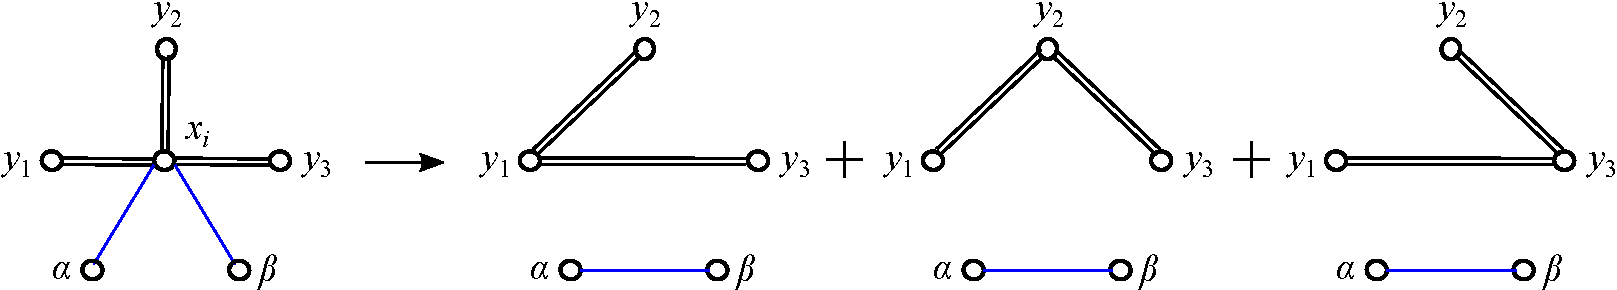
\includegraphics[width=12cm]{sumbedges.pdf}
\end{center}


% For this purpose, we first show the following bound:
%\be\label{keyobs3}
%\sum_{x_i} B_{y_1 x_i}\cdots B_{y_k x_i}\cal A^{(2)}_{x_i \beta}\prec W^{-ad/2 } \Gamma(y_1,\cdots, y_k).
%\ee
To prove \eqref{keyobs3}, it suffices to assume the weaker condition $\|\cal A^{(2)}\|_{w;(a,b)}\prec 1$. (When only $\|\cal A^{(2)}\|_{s;(a,b)}\prec 1$ is assumed, this uses that the weak-$(a,b)$ norm is bounded by a constant times the strong-$(a,b)$ norm, which requires $0\le ad/2-b<d$; this condition holds for all the pairs $(a,b)$ used in this paper, namely $(1,1)$, $(1,2)$, $(2,2)$ and $(2,4)$.) We decompose the sum over $x_i$ according to dyadic scales $K_n$ defined in \eqref{defn Kn}. Consider the case $x_i \in \cal I_{\vec a}$ for some $\vec a:=(a_1, \cdots, a_k)\in (\N\setminus\{0\})^k$, where 
$$\cal I_{\vec a}:=\{ x_i: K_{a_j-1} \le |x_i - y_j| \le K_{a_j} ,  1\le j \le k\}.$$ For simplicity of notations, we abbreviate $L_j := K_{a_j}$ and $L_{\min}:=\min_{1\le j \le k}L_j $. Then we have that 
\begin{align}\label{sum_ba}
\sum_{x_i \in \cal I_{\vec a}} |\cal A^{(2)}_{x_i \beta}|\cdot \prod_{j=1}^k B_{x_i y_j }\le \prod_{j=1}^k\frac{1}{W^2L_j^{d-2}} \sum_{x\in \cal I_{\vec a}}  |\cal A ^{(2)}_{x_i \beta}|  \prec   \frac{L_{\min}^{d}}{W^bL_{\min}^{ad/2-b} }\frac{1}{\prod_{j=1}^k W^2L_j^{d-2}} ,  
\end{align}  
where in the second step we used \eqref{eq PseudoG} and the fact that $\cal I_{\vec a}$ is inside a box of scale $L_{\min}$.
%\begin{align}
% K^{-d}\sum_{\al: |\al- w|\le K}\sum_{x_i \in \cal I_{\vec a}} B_{y_1 x_i}\cdots B_{y_k x_i}\cal A_{x_i \al}\cal A _{x_i \beta} &\prec \frac{1}{W^{1/2}K^{d/4-1/2}} \prod_{j=1}^k\frac{1}{W^2L_j^{d-2}} \sum_{x_i\in \cal I_{\vec a}}  \cal A _{x_i \beta} \label{verifypseudo1}\\
%&\prec  \frac{1}{W^{1/2}K^{d/4-1/2}}  \frac{(L_1\wedge L_2\wedge \cdots \wedge L_k)^{3d/4+1/2}W^{-1/2}}{\prod_{j=1}^k W^2L_j^{d-2}} . \nonumber
%\end{align}  
Let $s \in \{1,2,\cdots, k\}$ be the value such that $L_s=L_{\min}$. Using \eqref{a+b}, we obtain that
$$\frac{L_{\min}^{d}}{ W^b L_{\min}^{ad/2-b} } \frac1{W^2L_s^{d-2}} = \frac{1}{W^{b+2}L_{\min}^{ad/2-b-2}}\le W^{-ad/2}.$$
Combining this bound with the fact that  
\be\label{yj-s}\langle y_j - y_s \rangle \le W+ L_j + L_s \le 3L_j,\quad j \ne s, \ee  
we can bound \eqref{sum_ba} as 
 \begin{align}
 \sum_{x_i \in \cal I_{\vec a}} |\cal A^{(2)}_{x_i \beta}|\cdot \prod_{j=1}^k B_{x_i y_j } \prec W^{-ad/2} \prod_{j\ne s} \frac1{W^2L_j^{d-2}} \lesssim W^{-ad/2} \prod_{j\ne s} B_{y_j y_s} \le  W^{-ad/2}{\Gamma(y_1,\cdots, y_k)} . \nonumber
\end{align}  
Summing over all possible scales $\cal I_{\vec a}$, we conclude \eqref{keyobs3}.
% \begin{align*}
%\sum_{x_i} B_{y_1 x_i}\cdots B_{y_k x_i}\cal A_{x_i \beta} \prec  W^{-d/2} {\Gamma(y_1,\cdots, y_k)} , %\label{checkpseudo1}
%\end{align*}  
%which concludes \eqref{keyobs3}.
%In order to improve the $W^{-d/4+\e_0}$ factor to $W^{-d/2+\e_0}$, we again can use the arguments in Corollary \ref{cor: ini bound}. 
%This concludes \eqref{eq PseudoG} for $\wt A_{\al\beta}$. 
%\begin{align*}
%&\sum_{x_i \in \cal I_{\vec a}} B_{y_1 x_i}\cdots B_{y_k x_i}\cal A_{x_i \al}\cal A _{x_i \beta} \prec  \sum_{x_i\in \cal I_{\vec a}} B_{y_1 x_i}\cdots B_{y_k x_i}\cal A_{x_i \al}(B^{1/2}_{x_i \beta}+\wt\Phi) \\
%&\prec W^{\e_0}\frac{(L_1\wedge L_2\wedge \cdots \wedge L_k)^{3d/4+1/2}W^{-1/2}}{\prod_{j=1}^k W^2L_j^{d-2}} (B^{1/2}_{\al \beta}+\wt\Phi) \prec W^{-d/4+\e_0}\Gamma(y_1,\cdots, y_k)(B^{1/2}_{\al \beta}+\wt\Phi),
%\end{align*}
%where in the second and third steps we used similar arguments as in the proof for \eqref{checkpseudo1}. Again using the arguments in Corollary \ref{cor: ini bound}, we can improve the $W^{-d/4+\e_0}$ factor to $W^{-d/2+\e_0}$. This concludes \eqref{eq PseudoG2} for $\wt A_{\al\beta}$. 
%In sum, we have proved \eqref{keyobs} and \eqref{keyobs2}. 
%which can be stated in the more convenient form: 
%\be\label{keyobs2}
%\sum_{x_i} B_{y_1 x_i}\cdots B_{y_k x_i}\cal A_{x_i \al}\cal A _{x_i \beta} =W^{-d/2+\e_0} \Gamma(y_1,\cdots, y_k)\AIT_{\al\beta},
%\ee
%for a pseudo $G$ edge $\AIT_{\al\beta}$. 


Next we prove \eqref{keyobs2} when $\|\cal A^{(1)}\|_{w;(a,b)}+ \|\cal A^{(2)}\|_{w;(a,b)}\prec 1$.
Applying \eqref{eq PseudoG2} to $\cal A^{(1)}_{x_i\al}$ and using \eqref{keyobs3}, we get that
\begin{align*}
& %\sum_{x_i } B_{y_1 x_i}\cdots B_{y_k x_i}\cal A^{(1)}_{x_i \al}\cal A ^{(2)}_{x_i \beta} , \ 
\sum_{x_i} |\cal A^{(1)}_{x_i \al}|  |\cal A^{(2)} _{x_i \beta}|\cdot \prod_{j=1}^k B_{x_i y_j } 
\prec W^{-ad/2}\sum_{x_i }  |\cal A^{(2)} _{x_i \beta}|\cdot \prod_{j=1}^k B_{x_i y_j }  \prec W^{-ad }\Gamma(y_1,\cdots, y_k).
\end{align*}
Applying \eqref{eq PseudoG} to $\cal A^{(1)}_{x_i\al}$ and using \eqref{keyobs3}, we get that for any $x_0\in \Z_L^d$ and $  K \in [W, L/2]$,
\begin{align*}
 \frac{1}{K^d}\sum_{\al: |\al - x_0|\le K}\sum_{x_i} |\cal A^{(1)}_{x_i \al}|  |\cal A^{(2)} _{x_i \beta}|\cdot \prod_{j=1}^k B_{x_i y_j }  & \prec \frac{\sum_{x_i } |\cal A^{(2)} _{x_i \beta}|\cdot  \prod_{j=1}^k B_{x_i y_j } }{W^{b}K^{ad/2-b}}  \prec W^{-ad/2} \frac{\Gamma(y_1,\cdots, y_k)}{W^{b}K^{ad/2-b}}. 
\end{align*} 
We can obtain a similar estimate for the average over $\{\beta:|\beta-x_0|\le K\}$. The above two estimates imply that $  \|\cal A\|_{w;(a,b)}\prec 1$, where $\cal A$ is defined by
\be\label{keyobs_add}
\begin{split}
	{\cal A}_{\al\beta}:=\frac{W^{ad/2 }}{\Gamma(y_1,\cdots, y_k)}\sum_{x_i} |\cal A^{(1)}_{x_i \al}|  |\cal A^{(2)} _{x_i \beta}|\cdot \prod_{j=1}^k B_{x_i y_j } . 
\end{split}
\ee
This concludes \eqref{keyobs2} in one case.
%\eqref{eq PseudoG2} and \eqref{eq PseudoG} hold for $\cal A_{\al\beta}$, which means that $\cal A$ satisfies the level-$(a,b)$ averaged bound. 
%which concludes \eqref{keyobs}.
Then we prove \eqref{keyobs2} in the other case with $\|\cal A^{(1)}\|_{s;(a,b)}+ \|\cal A^{(2)}\|_{s;(a,b)}\prec 1$. We decompose the sum over $x_i$ according to dyadic scales as $x_i \in \cal I_{\vec a}$ for some $\vec a:=(a_1, \cdots, a_{k+2})\in (\N\setminus\{0\})^{k+2}$, where 
$$\cal I_{\vec a}:=\{ x_i: K_{a_j-1} \le |x_i - y_j| \le K_{a_j} ,  1\le j \le k; K_{a_{k+1}-1} \le |x_i-\al|\le K_{a_{k+1}}, K_{a_{k+2}-1} \le |x_i-\beta|\le K_{a_{k+2}}\}.$$ For simplicity of notations, we abbreviate $L_j := K_{a_j}$, $1\le j \le k+2$, and $L_{\min}:=\min_{1\le j \le k}L_j$. Let $s \in \{1,2,\cdots, k\}$ be the value such that $L_s=L_{\min}$. Then using \eqref{eq unifG} and the fact that $\cal I_{\vec a}$ is inside a box of scale $L_{\min}\wedge L_{k+1}\wedge L_{k+2}$, we obtain that 
\begin{align} \nonumber
& \sum_{x_i \in \cal I_{\vec a}} |\cal A^{(1)}_{x_i \al}|  |\cal A^{(2)} _{x_i \beta}|\cdot \prod_{j=1}^k B_{x_i y_j }    \prec \prod_{j=1}^k\frac{1}{W^2L_j^{d-2}} \cdot\frac{(L_{\min}\wedge L_{k+1}\wedge L_{k+2})^d}{W^{2b} L_{k+1}^{ad/2-b}L_{k+2}^{ad/2-b}} \\
&\le   \prod_{1\le j \le k, j\ne s}\frac{1}{W^2L_j^{d-2}} \cdot\frac{1}{W^{b} (L_{k+1}\vee L_{k+2})^{ad/2-b}}\cdot\frac{1}{W^{b+2}(L_{k+1}\wedge L_{k+2})^{ad/2-b-2}} \nonumber\\
& \lesssim W^{-ad/2} \frac{1}{W^{b} \langle \al-\beta \rangle^{ad/2-b}}\prod_{j\ne s} B_{y_j y_s}. \nonumber
\end{align}  
Here in the second step we used $L_{k+1} L_{k+2}=(L_{k+1}\vee L_{k+2})(L_{k+1}\wedge L_{k+2})$, and  in the third step we used \eqref{a+b}, \eqref{yj-s} and  $\langle \al - \beta \rangle \le W+ L_{k+1} + L_{k+2} \le 3L_{k+1}\vee L_{k+2} $. Summing the above estimate over all possible scales $\cal I_{\vec a}$, we get that $\|\cal A\|_{s;(a,b)}\prec 1$, which concludes \eqref{keyobs2}.

%\eqref{eq unifG} holds for $\cal A_{\al\beta}$, which means that $\cal A$ satisfies the level-$(a,b)$ pointwise bound. %In sum, we conclude \eqref{keyobs}. % together with the above proof for the case averaged bound.

%With the above observations, we can finally sum over the molecules on this path from $\cal M_{k_0}$ to $\cal M_b$ and conclude the proof.


Now the proof of \eqref{boundaux} involves repeated applications of \eqref{keyobs3} and \eqref{keyobs2} with a carefully chosen order of summations. Without loss of generality, we regard $y$ as the root of the blue tree, and sum over the internal vertices from the leaves of the blue tree to the root. More precisely, we will sum over the vertices according to a partial order $x_{i_1}\preceq x_{i_2} \preceq \cdots \preceq x_{i_\ell}\preceq y$ that is compatible with the blue tree structure---if $x_i$ is a child of $x_j$, then we have $x_i \preceq x_j$. %Here $i_1,\cdots, i_\ell$ is a permutation of $1,\cdots, \ell$. 
By renaming the labels of vertices if necessary, we can assume that the partial order is $x_1\preceq x_2  \preceq\cdots \preceq x_\ell$, so that we will perform the summations according to the order $\sum_{x_\ell}\cdots \sum_{x_2}\sum_{x_1}$. For simplicity of notations, we denote all the blue solid edges appearing in the proof by $\cal A$, including the old edges in  $\wt{\cal G}_{xy}$ and the new edges coming from applications of \eqref{keyobs2}. All these $\cal A$ variables have weak-$(a,b)$ or strong-$(a,b)$ norms bounded by $\OO_\prec(1)$, and their exact expressions may change from one line to another. 


For the summation over $x_1$, using \eqref{keyobs3} (if  $x_1$ is not connected with $x$ in the blue tree) or \eqref{keyobs2} (if $x_1$ is connected with $x$ in the blue tree), we can bound $\wt{\cal G}_{xy}$ as
\be\label{reduceaux1}\wt{\cal G}_{xy} \prec W^{-ad/2 }\sum_{k=1}^{\ell_1} \cal G^{(1)}_{xy,k},\ee
where $\cal G^{(1)}_{xy, k}$ are new graphs obtained by replacing the edges connected to $x_1$ with the graphs on the right-hand side of \eqref{keyobs3} or \eqref{keyobs2}, and $\ell_1$ is the number of neighbors of $x_1$ on the black tree. More precisely, we perform the following operations to get these new graphs. 
\begin{itemize}
	\item We get rid of the blue solid and black double-line edges connected with $x_1$. 
	\item If $x$ and $x_1$ are connected through a blue solid edge in $\wt{\cal G}_{xy}$, then in each new graph $x$ is connected to the parent of $x_1$ on the blue tree through a blue solid edge.
	\item Suppose $w_{1},\cdots,w_{\ell_1}$ are the neighbors of $x_1$ on the black tree. Then corresponding to the $k$-th term in $\Gamma(w_{1},\cdots, w_{\ell_1})$, $k=1,\cdots, \ell_1$, the atoms $w_{1},\cdots,w_{k-1},w_{k+1},\cdots, w_{\ell_1}$ are connected to $w_{k}$ through double-line edges in the new graph. 
\end{itemize}
Now it is crucial to observe that each new graph \smash{$\cal G^{(1)}_{xy,k}$} is still doubly connected. % that is, there are blue and black trees, each of which connects all the atoms $x,y, x_2,\cdots, x_\ell$. 
In \eqref{Graphreduction}, we show the reduction from the first graph to the second one through a summation over $x_1$, where we have omitted the factor $W^{-ad/2}$ from the graphs.
%\begin{center}
\be  \label{Graphreduction}
\parbox[c]{0.9\linewidth}{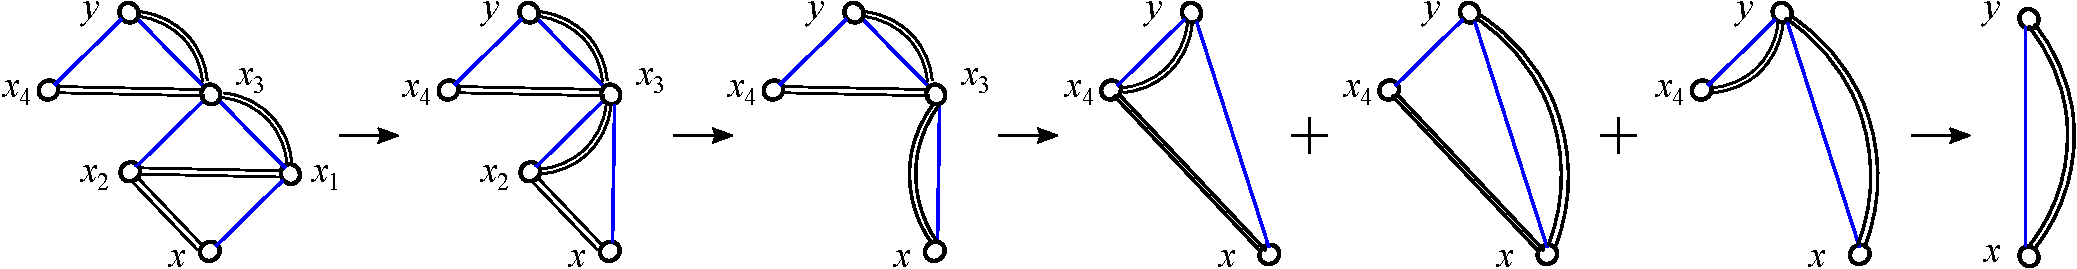
\includegraphics[width=\linewidth]{Graphreduction2.pdf}} 
\ee
%\end{center}
Similarly, we can bound the summations over atoms $x_2, \cdots , x_{\ell}$ one by one using \eqref{keyobs3} and \eqref{keyobs2}. At each step we gain an extra factor $W^{-ad/2}$ and reduce the graphs into a sum of several new graphs, each of which has one fewer atom and a doubly connected structure. Finally, after summing over all internal atoms, we obtain a graph with atoms $x$ and $y$ only. In this case, the only doubly connected graph is the graph where $x$ and $y$ are connected by a double-line $B_{xy}$ edge and a blue solid edge whose weak-$(a,b)$ or strong-$(a,b)$ norm is bounded by $\OO_\prec(1)$. This concludes \eqref{boundaux}. In \eqref{Graphreduction}, we give an example of the above graph reduction process by summing over the four internal atoms.

In the case of weak norms, the above argument needs a modification. The variable $\cal A$ defined in \eqref{keyobs_add} depends also on the positions $y_1,\cdots,y_k$ of the neighbors of $x_i$ on the black tree, while its weak-$(a,b)$ norm is only controlled for fixed $y_1,\cdots,y_k$. Hence \eqref{keyobs3} and \eqref{keyobs2} cannot be applied to such a blue edge in a later summation over an atom among $y_1,\cdots,y_k$, and the final variable $\cal A_{xy}$ may depend on $x$ and $y$ also through these positions. (This issue does not occur for strong norms, since in that case the new blue edge is bounded pointwise by the fixed matrix $W^{-b}\langle \al-\beta\rangle^{-(ad/2-b)}$.) Therefore, for weak norms we prove \eqref{boundaux} without using \eqref{keyobs2}: we only use \eqref{keyobs3}, \eqref{eq PseudoG2} and \eqref{eq PseudoG} for the original blue edges of $\wt{\cal G}_{xy}$, which are fixed matrices with weak-$(a,b)$ norms bounded by $\OO_\prec(1)$. Let $\cal A_{xy}:=W^{a\ell d/2}\wt{\cal G}_{xy}/B_{xy}$. By Definition \ref{Def PseudoG}, $\|\cal A\|_{w;(a,b)}\prec 1$ follows from the following two estimates: 
\begin{itemize}
\item[(a)] $\wt{\cal G}_{xy}\prec W^{-a(\ell+1)d/2}B_{xy}$ uniformly in $x,y\in\Z_L^d$;
\item[(b)] $\sum_{y:|y-x_0|\le K}\wt{\cal G}_{xy}/B_{xy}\prec W^{-a\ell d/2}K^{d}W^{-b}K^{-(ad/2-b)}$ uniformly in $x,x_0\in\Z_L^d$ and $K\in[W,L/2]$, and the same estimate holds with the roles of $x$ and $y$ exchanged.
\end{itemize}
To prove (a), we regard $y$ as the root of the blue tree, bound the blue edge between $x$ and its parent by its maximum $\OO_\prec(W^{-ad/2})$ using \eqref{eq PseudoG2}, and then sum over the internal atoms in an order compatible with the blue tree as above. When we sum over an internal atom $x_i$, the blue edges between $x_i$ and its children have been removed in the previous steps, so $x_i$ is connected to the other atoms only through its blue edge to its parent, which is an original blue edge, and through its black edges. Moreover, the black edges always form a spanning tree of the remaining atoms (in the bound \eqref{keyobs3}, the neighbors $y_1,\cdots,y_k$ of $x_i$ are connected by the double-line edges in $\Gamma(y_1,\cdots,y_k)$), so $x_i$ has at least one black edge. Hence \eqref{keyobs3} applies to every summation and gives a factor $W^{-ad/2}$. After summing over all the $\ell$ internal atoms, we obtain $\OO(1)$ many graphs, each consisting of the double-line edge $B_{xy}$, which concludes (a).

To prove (b), we fix $x$, $x_0$ and $K$. Let $e_1,\cdots,e_h$, $h\le \ell+1$, be the black edges on the path between $x$ and $y$ in the black tree, and denote $\langle e\rangle:=\langle \al-\beta\rangle$ for an edge $e$ between atoms $\al$ and $\beta$. By the triangle inequality, $\langle x-y\rangle \le \sum_{i}\langle e_i\rangle\le h\max_i\langle e_i\rangle$, which gives $B_{xy}^{-1}\le h^{d-2}\sum_{i=1}^h B_{e_i}^{-1}$. Hence it suffices to prove (b) with $\wt{\cal G}_{xy}/B_{xy}$ replaced by the graph $\wt{\cal G}^{(i)}_{xy}$ obtained by removing the black edge $e_i$ from $\wt{\cal G}_{xy}$. After this removal, the black tree splits into two trees containing $x$ and $y$, respectively. We now regard $x$ as the root of the blue tree, and sum over the internal atoms and the atom $y$ one by one in an order compatible with the blue tree (from the leaves to the root), where $y$ is summed over the box $\{y:|y-x_0|\le K\}$ and the internal atoms are summed over $\Z_L^d$. At each step, the atom, say $w$, that we sum over is connected to the other atoms only through its blue edge to its parent and its black edges. At any time, at most one atom is restricted to a box, and we call it the box atom (initially, it is $y$ with the box of radius $K$ around $x_0$). 
\begin{itemize}
\item If $w$ is not the box atom, then we sum over $w\in\Z_L^d$ using \eqref{keyobs3}, which gives a factor $W^{-ad/2}$. Here $w$ has at least one black edge, because, as shown below, every black component of the remaining graph contains $x$, a fixed point $z_0$, or the box atom.

\item If $w$ is the box atom with the box $\{w:|w-z_0|\le K'\}$, let $u_1,\cdots, u_j$ be its neighbors on the black tree, and use $1\le \mathbf 1(|u_i-z_0|>2K' \text{ for all } i)+\sum_{i}\mathbf 1(|u_i-z_0|\le 2K')$. On the first event, we have $\langle w-u_i\rangle\ge \langle z_0-u_i\rangle/2$ and hence $B_{wu_i}\le 2^{d-2}B_{z_0u_i}$ for all $i$; we replace the black edges $B_{wu_i}$ with $2^{d-2}B_{z_0u_i}$, i.e., we move them to the fixed point $z_0$, and then sum over $w$ in the box using \eqref{eq PseudoG} for its blue edge, which gives a factor $\OO_\prec(K'^dW^{-b}K'^{-(ad/2-b)})$. On the event $|u_i-z_0|\le 2K'$, we sum over $w\in \Z_L^d$ using \eqref{keyobs3}, which gives a factor $W^{-ad/2}$, and $u_i$ becomes the new box atom with the box $\{u_i:|u_i-z_0|\le 2K'\}$ (if $2K'>L/2$, this box is the whole torus, and we take $K'=L/2$ in the next step). 
\end{itemize}
After the removal of $e_i$, the black component containing the box atom does not contain $x$, and the above operations keep the following properties: every black component contains $x$, the fixed point $z_0$ (after the first event), or the box atom; the black component containing the box atom contains neither $x$ nor $z_0$. In particular, a box is passed only to internal atoms, at most $\ell$ times, so that $K'\le 2^\ell K$. Moreover, in each of the resulting $\OO(1)$ many terms, exactly one atom is summed over a box and the other $\ell$ atoms are summed over $\Z_L^d$, and the remaining black edges, which connect $x$ and $z_0$, are bounded by $1$. Since $K'^{d-(ad/2-b)}\le 2^{\ell d}K^{d-(ad/2-b)}$ by $0\le ad/2-b<d$, we obtain the first estimate in (b). The second estimate in (b) follows from the same argument with the roles of $x$ and $y$ exchanged. Here the logarithmic factors from the dyadic decompositions in the proofs of \eqref{keyobs3} are bounded by $(\log L)^C\prec 1$. This concludes \eqref{boundaux} for weak norms.
%In the end, 
%$$(\cal G_{xy})_{aux} \prec W^{-ad\ell /2}B_{xy}\cal A_{xy}.$$
%This proves \eqref{boundaux}, which further concludes \eqref{bound 2net1}.  
\end{proof}

%\iffalse
%\begin{remark}
%We only combine the molecules for the purpose of this proof. In the graph expansions, we generally keep the dotted edges and do not combine different molecules in order to keep track of the graph structure in a clearer way. %in some unwanted way. %(\cor will rethink about this\nc). 
%\end{remark}
%\fi
 

%\begin{corollary}\label{order cor}
%Given a graph with dashed black $b^{(1)}$ edges and solid blue $G$ edges, if we can use (some of the) blue edges to build an oriented tree that connects all the molecules, then Theorem \ref{order thm} holds. As a special case, Theorem \ref{order thm} holds if there exists a blue edge path that connects all the molecules.
%\end{corollary}
%
%\begin{proof}
%The second statement is a special case of the first one, because a path is a 1-regular tree. Now we prove the first statement. We only need to prove that \eqref{order eq} holds. 
%
%We define the depth of a molecule as its graph distance to the root. Let $L$ be the depth of the tree (i.e. the depth of the deepest molecule). Then we define an order ``$<$" of the molecules in the following way. For the molecules with different depth, we have
%$$\cal M_i < \cal M_j \quad \text{if} \quad \text{depth}(\cal M_i) > \text{depth}(\cal M_j) .$$
%For the molecules with the same depth, we fix an arbitrary order of them. Let $\pi$ be such that $\cal M_{\pi(1)} < \cal M_{\pi(2)} < \cdots < \cal M_{\pi(n)}$, then we have \eqref{order eq} holds because for any molecule $\cal M_{\pi(i)}$, it is connected to its parent $\cal M_{\pi(t)}$ through a blue edge. By definition of the order, we have $t>s$. 
%\end{proof}


%From Lemma \ref{no dot}, we immediately obtain the following corollary, 

If $\|G(z)-m(z)I_N\|_{w;(1,2)} \prec W^{\e_0} $ for a constant $0\le \e_0< d/2$, then applying \eqref{bound 2net1} on the event $\{\|G(z)-m(z)I_N\|_{w;(1,2)}\le W^{\e_0+\tau}\}$ with $\Lambda=W^{\e_0+\tau}$ for an arbitrarily small constant $\tau\in (0, d/2-\e_0]$, we immediately get that %the slightly weaker bounds \eqref{Gmax} and \eqref{initial Txy222} than the level-$(1,2)$ averaged bound due to the extra factor $W^{\e_0}$. 
\be\label{bound 2net1 cor}
\left|\cal G_{xy}\right| \prec W^{(n_{xy}-2)\e_0}\cdot  W^{ -  \left(n_{xy}-3\right)d/2} B_{xy} \cal A_{xy},
\ee
for a positive variable $\cal A_{xy}$ satisfying $\|\cal A\|_{w;(1,2)}\prec 1$. %where $n_{xy}:=\ord(\cal G_{xy})$ and $\cal A_{xy}$ is a positive variable satisfying the level-$(1, 2)$ averaged bound.
Here $\prec$ is understood in the sense of Definition \ref{stoch_domination} (i), and the factor $W^{(n_{xy}-2)\e_0}$ comes from the factor $\Lambda^{n_{xy}-2}$ in \eqref{bound 2net1}, i.e., from the fact that the number of light weights and off-diagonal $G$ edges in $\cal G_{xy}$ is at most $n_{xy} -2$.

% \begin{corollary}\label{no dot cor}
% Suppose $d\ge 8$ and $\|G(z)-m(z)I_N\|_{w;(1,2)}\prec 1$. 
% %that $W^{-\e_0}|G_{xy}(z)-m(z)\delta_{xy}|$ satisfies the level-$(1,2)$ averaged bound for a constant $\e_0>0$. 
% Let $\cal G$ be a doubly connected normal regular graph without external atoms as in Definition \ref{def 2net}. 
%Pick any two atoms of $\cal G$ and fix their values $x , y\in \Z_L^d$. Then for the resulting graph, say $\cal G_{xy}$, we have that
%\be\label{bound 2net1 cor}
%\left|\cal G_{xy}\right| \prec W^{(n_{xy}-2)\e_0}\cdot  W^{ -  \left(n_{xy}-3\right)d/2} B_{xy} \cal A_{xy},
%\ee
%where $n_{xy}:=\ord(\cal G_{xy})$ and $\cal A_{xy}$ is a positive variable satisfying the level-$(1, 2)$ averaged bound.
% \end{corollary}
% \begin{proof}
% By Lemma \ref{no dot} on $\cal G^{\rm abs}_{xy}$, we have that 
%$$ \left|\cal G_{xy}\right| \le  W^{k \e_0} \cdot \cal G^{\rm abs}_{xy} \prec W^{k \e_0}\cdot  W^{ -  \left(n_{xy}-3\right)d/2} B_{xy} \cal A_{xy}, $$
%where $k$ is the number of light weights and off-diagonal $G$ edges in $\cal G_{xy}$.  %Recall that for the normal regular graphs in Definition \ref{defnlvl0}, each atom is connected with at least one waved or $\dashed$ edge. Moreover, there are two external atoms in $\cal G_{xy}$. 
%Due to property (iii) of Definition \ref{defnlvl0}, the number of internal atoms in $\cal G_{xy}$ is smaller than the number of waved and $\dashed$ edges at least by 1. Hence by definition \eqref{eq_deforderrandom3}, we obtain that $k \le n_{xy} -2$, which concludes \eqref{bound 2net1 cor}.
% \end{proof}

Deterministic doubly connected graphs satisfy better bounds than Lemma \ref{no dot}, because all edges in the blue net are now (labelled) $\dashed$ edges, whose strong-$(2,2)$ norms are bounded by $\OO_\prec(1)$.%satisfy the better level-$(2,2)$ pointwise bound. 
 
 


\begin{corollary}\label{lem Rdouble}
Suppose $d\ge 6$. Let $\cal G$ be a deterministic doubly connected normal regular graph without external atoms. Pick any two atoms of $\cal G$ and fix their values as $x , y\in \Z_L^d$. Then the resulting graph $\cal G_{xy}$ satisfies that %for any constant $\e>0$,
\be\label{bound 2net1B}
\left|\cal G_{xy}\right| \prec W^{ - \left(n_{xy} -4\right) d/2} B_{xy}^2 ,\quad \text{with}\quad n_{xy}:=\ord(\cal G_{xy}).
\ee
This bound also holds for the graph $ {\cal G}^{{\rm abs}}_{xy}$. % which is obtained by replacing each component (including edges and coefficients) in $\cal G_{xy}$ with its absolute value. 
\end{corollary}
\begin{proof} 
This corollary can be proved in the same way as Lemma \ref{no dot}, except that we need to apply Claim \ref{twonet claim} to an auxiliary graph whose blue edges have strong-$(2,2)$ norms bounded by $\OO_\prec(1)$. %Note that taking $a=b=2$ in the condition \eqref{a+b} gives  $d\ge 4$.
%As in the proof of Lemma \ref{no dot}, we first combine all the atoms in $\cal G_{xy}$ that are connected through dotted edges, and obtain a new graph. Then this new graph is still a doubly connected deterministic graph and has no dotted edges between different molecules. Following the arguments in the proof of Lemma \ref{no dot}, it suffices to bound a doubly connected deterministic auxiliary graph $(\cal G_{xy})_{aux}$ with a black spanning tree and a blue spanning trees, where each black or blue edge represents a $B$ edge. We claim that after summing over all the internal atoms in $ (\cal G_{xy})_{aux}$, the auxiliary graph can be bounded by
%\be\label{boundauxB}
%| (\cal G_{xy})_{aux}| \prec W^{-d\ell }B^2_{xy}, \quad \ell:=\#\{\text{internal atoms in } (\cal G_{xy})_{aux}\}  .
%\ee
%Similar to \eqref{keyobs2}, we can prove that 
%\be\label{keyobs2BB}
%\sum_{x_i} B_{y_1 x_i}\cdots B_{y_k x_i}B_{x_i \al}B _{x_i \beta}  \lesssim W^{-d}\Gamma(y_1,\cdots, y_k) B_{\al\beta}
%\ee
%with a similar (actually easier) argument. With \eqref{keyobs2BB}, we can perform a similar graph reduction argument as the one around \eqref{reduceaux1}. After summing over all atoms, we can reduce the graph into two $B$ edges between $x$ and $y$. Furthermore, for each summation over an internal atom, we gain a $W^{-d}$ factor. Thus we conclude \eqref{boundauxB}, which further implies \eqref{bound 2net1B} as we have seen in the proof of Lemma \ref{no dot}.  
\end{proof}


 We also need another version of Corollary \ref{lem Rdouble}, which will be used in the proof of Lemma \ref{lem V-R wt} in Section \ref{subsec_inf_pf} below.
\begin{corollary}\label{lem Rdouble weak}
Under the assumptions of Corollary \ref{lem Rdouble}, suppose we replace every (labelled) $\dashed$ edge in $\cal G$ between atoms, say $\al$ and $\beta$, with an edge bounded by $\OO_\prec (B_{\al\beta})$, that is, by $W^{\tau}B_{\al\beta}$ for any constant $\tau>0$ (in the sense of Definition \ref{stoch_domination} (ii)). We treat these edges as double-line edges of scaling order $2$ and call the resulting graph $\cal G'$. We pick any two atoms of $\cal G'$ and fix their values as $x , y\in \Z_L^d$. Then the resulting graph  $\cal G'_{xy}$ satisfies the bound %if $d\ge 4$: 
\be\label{bound 2net weak0}
\left|\cal G'_{xy}\right| \le \frac{W^{ - \left(n'_{xy}-4\right) d/2}}{W^4\langle x-y\rangle^{2d-4-\tau}} ,
\quad \text{with }\ \ n'_{xy}:=\ord(\cal G'_{xy}),
\ee
for any constant $\tau>0$. Furthermore, suppose we replace exactly one double-line edge, say between atoms $ \al_0$ and $ \beta_0$, in $\cal G'_{xy}$ with an edge bounded by {$\OO_\prec (\wt B_{\al_0 \beta_0})$}, where \smash{$\wt B_{ \al_0 \beta_0}:= W^{-4}\langle \al_0 - \beta_0\rangle^{-(d-4)}.$}
%Moreover, we replace any other (labelled) $\dashed$ edge between atoms, say $\al$ and $\beta$, with an edge bounded by $\OO_\prec (B_{\al\beta})$. 
We treat this edges as a double-line edge of scaling order $2$ and denote the resulting graph by $\cal G''_{xy}$. %Then pick any two atoms of $\cal G''$ and fix their values as $x , y\in \Z_L^d$. For the resulting graph, say $\cal G'_{xy}$, 
Then it satisfies the bound %holds if $d\ge 6$: 
\be\label{bound 2net weak}
\left|\cal G''_{xy}\right| \le  \frac{W^{ - \left(n''_{xy}-4\right) d/2}}{W^6\langle x-y\rangle^{2d-6-\tau}},\quad \text{with }\ \ n''_{xy}:=\ord(\cal G''_{xy}),
\ee
for any constant $\tau>0$.
%where $$. %is the scaling order of $\cal G'_{xy}$ with the new edge counted as an edge of order 2.
\end{corollary}
\begin{proof}
The estimate \eqref{bound 2net weak0} follows from \eqref{bound 2net1B}. The estimate \eqref{bound 2net weak} can be proved in the same way as Lemma \ref{no dot}, except that we need to apply Claim \ref{twonet claim} to an auxiliary graph whose blue edges have strong-$(2,4)$ norms bounded by $\OO_\prec(1)$. Here we can assume that the edge bounded by $\OO_\prec (\wt B_{\al_0 \beta_0})$ belongs to the blue net: otherwise, we exchange the black and blue nets, which is possible since both nets of the deterministic graph $\cal G''_{xy}$ consist of double-line edges.
%with blue edges satisfying the level-$(2,4)$ pointwise bound. 
%Note that taking $a=2$ and $b=4$ in the condition \eqref{a+b} gives $d\ge 6$.
%The proof is the same as \eqref{lem Rdouble}, except that we replace \eqref{keyobs2BB} with 
%\be \nonumber%\label{keyobs2BB}
%\sum_{x_i} B_{y_1 x_i}\cdots B_{y_k x_i}B_{x_i \al}\wt B _{x_i \beta}  \lesssim W^{-d}\Gamma(y_1,\cdots, y_k) \wt B_{\al\beta}
%\ee 
%if the new edge is used in the black or blue spanning tree. Hence at the end of the graph reduction of the auxiliary graph, we obtain a graph with $B$ and $\wt B$ edges between $x$ and $y$. This gives \eqref{bound 2net weak}.
\end{proof}

%\cob
%Before the end of this section, we discuss the issue with the dashed-dotted edges between different molecules. We claim that each dashed-dotted edge behaves as a grey edge (i.e. it can be either used as a blue edge or a black edge).  We prove the following version of Theorem \ref{order thm} but with dashed-dotted edges between molecules. 
% 
% 
% \begin{theorem}\label{order thm2}
%Consider a graph with molecules $\cal M_1,\cal M_2,\cdots, \cal M_n$, $\mu,\nu$ and a given set of molecules $J$. Suppose $\cal M_1,\cal M_2,\cdots, \cal M_n$ form a molecule family tree with root $\mu$ and edges given by black edges. Suppose there exists a partial order of all molecules $\pi: S_n \to S_n$ such that the following holds:
%\be\label{order eq2}
%\begin{split}
%& \text{ $\forall \; 1\le s\le n$, either there is a dashed-dotted edge connecting $\cal M_s$ with $J$, or there exists $t>s$ } \\
%& \text{such that there exists one $G$ edge or dash-dotted edge between molecule $\cal M_{\pi(s)}$ and $\cal M_{\pi(t)}$,}
%\end{split}
%\ee
%where we adopt the convention $\nu:= \cal M_{\pi(n+1)}$ with $\pi(n+1)=n+1$. Then after summing over all these molecules with order $\pi(1)\to \pi(2) \to \cdots \to \pi(n)$, the graph is at most of the order 
%$$\OO_\prec\left(W^{- \frac{1}{2}  nd  }\right).$$ 
%\end{theorem}
%
%\begin{proof}
%The proof is similar to that for Theorem \ref{order thm}. Without loss of generality, we assume that $\pi= (1,2,\cdots, n)$. Again we consider the family tree of black $\dashed$ edge, where each of the edge in the tree is of a fixed scale. We label the edges by $e_i=(\cal M_{\al(i)}, \cal M_{\beta(i)})$, with 
%$$K_i \le \text{dist}(\cal M_{\al(i)}, \cal M_{\beta(i)}) \le 2K_i.$$
%We will also use the notation $K_{\al(i)\beta(i)}\equiv K_i$. It is easy to see the black dashed $b^{(1)}$ edges between these molecules provides a factor of order
%\be \nonumber %\label{initiale1} 
%\OO_\prec \left( \prod_{i=1}^n \frac{1}{W^2 K_i^{d-2}}\right).\ee
%
%Next we sum over the molecules according to the order $(1,2,\cdots, n)$. We denote
%$$L_1 = K_{1k_1} =\min_{i:\cal M_i \sim \cal M_1} K_{1i}, \quad \cal M_{k_1}\sim \cal M_1.$$
%If there is a dashed-dotted edge connected with $\cal M_1$, then the summation gives a factor $\OO(1)$. If there is no dashed-dotted edge connected with $\cal M_1$, then there is a $G$ edge between $\cal M_1$ and the molecule, say $\cal M_{i_1}$. As we have seen before, summing over this $G$ edge gives that
%$$\OO_\prec \left(\frac{W^2L_1^{d-2}}{W^{d/2}}+\min\left\{ \frac{L_1^d}{ W^d}, \frac{W^2 L_1^{d-2}}{W^{\frac52}L_1^{\frac{d}{4}-\frac52}}\right\}\right).$$
%%using \eqref{initial0} and $\wt\Phi=W^{-d}$. 
%Note that the $\OO(1)$ factor in the case with dashed-dotted edge can be also bounded by this factor. Then the rest of the proof is the same as the one for Theorem \ref{order thm}.
%\end{proof}
%
%\begin{corollary}\label{order thm3}
%Suppose the assumptions of Theorem \ref{order thm2} hold, except that we replace some black edges on the molecule family tree with dash-dotted edges. Then we have that the graph is at most of the order 
%$$\OO_\prec\left(W^{- \frac{1}{2}  kd  }\right),$$
%where $k$ is the number of molecules that are connected with black or blue edges. 
%\end{corollary}
%\begin{proof}
%This corollary follows directly from Theorem \ref{order thm2} by combining the molecules that are connected through dash-dotted edges on the molecule family. Notice that after combination of the molecules, we still have a molecule family tree structure and the graph satisfies the assumptions of Theorem \ref{order thm2}.  
%\end{proof}

\subsection{Proof of Lemma \ref{lem informal}}\label{secpfinformal}



%\begin{proof}[Proof of Lemma \ref{lem informal}]
%\subsection{A model system.}\label{sec inductiononn}\ 
%In this section, we prove \eqref{small SnE2} for a model system with a carefully chosen system size. The main task to prove the following claim.
%
%\begin{claim}\label{claim maincancel}
%Suppose the assumptions of Lemma \ref{lemm V-R} hold, and that for all $2l\le n-1$,
%\be\label{lowercancel} \sum_x (\cal V^{(n)}_{2l})_{x0} =0.\ee
%Let $L$ satisfy
%\be\label{Lcondition1} W^{(n/2-3/2)d+c_0} \le {L^2}/{W^2}  \le W^{(n/2-1)d-c_0} \ee
%for some constant $c_0>0$, and $\eta_n=W^{2+\e}/L^2$ for some small enough constant $\e>0$. Then we have 
%\be\label{small SnE3}
%\begin{split}
% \sum_{x,y} (R_{n}^{(n)})_{xy} (f,m(E+\ii \eta),S, S^{\pm}(z),\Theta(z)) \le N(W^{-c} W^{-(n/2-1)d} )
%\end{split}
%\ee
%for some constant $c>0$.
%\end{claim}
%
%To prove this claim, we will need the following version of Theorem \ref{main thm}, which is stated for random band matrices with system sizes satisfying the upper bound in \eqref{Lcondition1}. Its proof is based on the $(n-1)$-th order $T$-expansion together with a high moment bound on $T_{xy}$, which will be given in Section \ref{sec ptree}.
%
%\begin{theorem}\label{thm ptree1}
%Suppose for all $2l\le k \le n-1$, properties \eqref{two_properties0R}-\eqref{3rd_property0R} hold for $R_{2l}^{(k)}$. Assume that $L$ satisfies 
%\be\label{Lcondition2}  {L^2}/{W^2}  \le W^{(n/2-1)d-c_0} \ee
%for some constant $c_0>0$. Then for any constant $\e>0$, the estimate \eqref{locallaw} holds uniformly for all $z= E+\ii\eta$ with $\eta\ge W^{2+\e}/L^2$.
%\end{theorem}
%
%Next we prove Claim \ref{claim maincancel} based on Theorem \ref{thm ptree} and the $n$-th order incomplete $T$-expansion in Definition \ref{mlevelT}.
%\begin{proof}[Proof of Claim \ref{claim maincancel}]
%Apply the $n$-th order $T$-expansion \eqref{mlevelT} to the $T$-variable $T_{\fa\fb}$, we get 
%\be\label{after1-5n}
% T_{\fa\fb}= m \Theta_{\fa \fb} \overline G_{\fb\fb} + \sum_x \left(\Theta \wt S^{(n)}_ \Delta \right)_{\fa x}|G_{x\fb}|^2   + (\PITn)_{\fa,\fb} +  (\AIT^{(n)}_{ho})_{\fa,\fb} + (\wt{\cal G}_{Q}^{(n)})_{\fa,\fb} + \OO_\prec(L^{-D}).
%\ee
%Summing over $\fa,\fb\in \Z_L^d$ and taking expectation, we obtain that the left-hand side of \eqref{after1-5n} gives
%\begin{align}\label{Rcancel1}
%&\sum_{\fa,\fb} \mathbb E T_{\fa\fb}(z) = |m|^2 \frac{ \sum_{x} \mathbb E\im G_{xx}}{\eta_n} =N |m|^2 \frac{ \im m + \OO_\prec(W^{-d/2})}{\eta_n},   
%\end{align}
%where we used Ward's identity in the second step, and Theorem \ref{thm ptree} in the third step. On the other hand, for the right-hand side of \eqref{after1-5n} we calculate the sum and expectation over each term. First, it is trivial to have $\E  (\wt{\cal G}_{Q}^{(n)})_{\fa,\fb}=0$. Using the definition of $\Theta$ in 
%\eqref{Thetapm}, we get
%\begin{align}\label{Rcancel2}
%\E\sum_{\fa,\fb} m \Theta_{\fa \fb} \overline G_{\fb\fb} =\sum_{\fa,\fb} \left(|m|^2+ \OO_\prec(W^{-d/2}) \right)\Theta_{\fa \fb}   = N\frac{|m|^4+\OO_\prec(W^{-d/2})}{1-|m|^2} .
%\end{align}
%Using \eqref{lowercancel} and \eqref{V-R2}, we can calculate that  
%\begin{align*}
%\E\sum_{l: 4\le 2l\le n-1}\sum_{\fa,\fb,x} \left(\Theta R^{(n)}_{2l} \right)_{\fa x}|G_{x\fb}|^2 &=\frac{|m|^2}{1-|m|^2}  \sum_{l: 4\le 2l\le n-1}\sum_{x,y} \left(R^{(n)}_{2l} \right)_{xy}\frac{\im m + \OO_\prec(W^{-d/2})  } 
%{\eta_n} \\
%&\prec N\eta_n W^{-d}\cdot \frac{|m|^2}{1-|m|^2}\cdot \frac{\im m}{\eta_n} \lesssim N\frac{W^{-d}}{\eta_n}.
%\end{align*}
%Together with $\wt S^{(n)}_\Delta=R_n^{(n)}+\sum_{2l\le n-1} \Theta R^{(n)}_{2l}$, we obtain that 
%\be\label{Rcancel3}
%\E \sum_{\fa,\fb,x} \left(\Theta \wt S^{(n)}_ \Delta \right)_{\fa x}|G_{x\fb}|^2 = \sum_{x,y} \left(R^{(n)}_{n} \right)_{xy} \cdot \frac{|m|^2}{1-|m|^2} \cdot \frac{\im m + \OO_\prec(W^{-d/2})  } {\eta_n}+ \OO_\prec\left( N\frac{W^{-d}}{\eta_n}\right).
% \ee
 %Recall that as discussed in Remark \ref{remark_upper}, the local law \eqref{locallaw} holds for $G(z_n, f, W, L_n)$ by Theorem \ref{thm ptree}. 
In this subsection, we complete the proof of Lemma \ref{lem informal} using the bounds on individual graphs in Claim 8.6 of \cite{PartII_high}, which are based on Lemma \ref{no dot}. Recall that by Theorem \ref{thm ptree}, the local law \eqref{locallaw1} holds for $G(z_n, \psi, W, L_n)$. Hence for any constant $\e_0>0$, the event $\{|G_{xy}(z_n)-m(z_n)\delta_{xy}|\le W^{\e_0}B_{xy}^{1/2},\ \forall\, x,y\in \Z_{L_n}^d\}$ holds with high probability; in particular, $\|G(z_n)-m(z_n)I_N\|_{s;(1,1)}\prec 1$. For simplicity of notations, in the following proof we abbreviate $G\equiv G(z_n, \psi, W, L_n)$. Moreover, in the setting of Lemma \ref{lem informal}, $\otimes$ represents the external atom $\fa$, while $\oplus$ and $\ominus$ both represent the external atom $\fb$. On the above event, we apply Claim 8.6 of \cite{PartII_high} to the graphs of the $n$-th order $\incomp$, which satisfy the properties in Definitions \ref{defn incompgenuni} and \ref{def incompgenuni} and Definition 6.3 of \cite{PartII_high}. Since $\e_0$ can be arbitrarily small, the factors $W^{C_{\cal G}\e_0}$ there can be absorbed into $\prec$. We will also use that
$$\sum_{\fb}B_{\fa\fb}\le C\frac{L_n^2}{W^2}=C\frac{W^{\e}}{\eta_n}.$$

We first consider the graphs in $(\PITn)_{\fa,\fb_1\fb_2}$ and the $\oplus/\ominus$-recollision graphs in $(\AITn)_{\fa,\fb_1\fb_2}$. Take such a graph, say $\cal G$. These graphs have scaling order $\ge 3$, and scaling order $\ge 5$ if $\oplus$ and $\ominus$ are connected through dotted edges (by Definition 6.3 of \cite{PartII_high}), so we have $n_{\cal G}\ge 3$. By Claim 8.6 (ii) of \cite{PartII_high}, we have $|\cal G_{\fa,\fb\fb}|\le \cal G^{\rm abs}_{\fa,\fb\fb}\prec W^{-(n_{\cal G}-2)d/2}B_{\fa\fb}$. Summing over $\fa$ and $\fb$, we obtain \eqref{intro_recol}. 

The graphs in $(\AITn)_{\fa,\fb_1\fb_2}$ and $(\Err_{n,D}')_{\fa,\fb_1\fb_2}$ without internal atoms are not covered by Claim 8.6 (ii)--(iii) of \cite{PartII_high}, and we bound them directly. Let $\cal G$ be such a graph. Its atoms are $\otimes$, $\oplus$ and $\ominus$. By properties (i) and (ix) of \cite[Definition 3.2]{PartII_high}, which also hold for the graphs in the $\incomp$ (see \cite[Definition 3.3]{PartII_high}), the only component at $\otimes$ is a $\dashed$ or labelled $\dashed$ edge between $\otimes$ and $\oplus$ or $\ominus$, and the dotted edges contain no cycles, so there is at most one dotted edge, which connects $\oplus$ and $\ominus$. At $\fb_1=\fb_2=\fb$, the edge at $\otimes$ is bounded by $W^{-(k-2)d/2+\tau}B_{\fa\fb}$ using \eqref{thetaxy} and \eqref{BRB}, where $k$ is its scaling order and $\tau>0$ is arbitrary. Every other component becomes a factor at $(\fb,\fb)$: a solid edge vanishes because of its $\times$-dotted edge (by property (iv) of Definition \ref{defnlvl0}), a light weight is $\OO_\prec(W^{-d/2})$ by \eqref{locallaw1}, a regular weight is $\OO_\prec(1)$, a waved, $\dashed$ or labelled $\dashed$ edge of scaling order $k'$ is $\OO_\prec(W^{-k'd/2})$ by \eqref{Ssmall}, and the dotted edge is equal to $1$. Since $\cal G$ has no internal atoms, the scaling orders of these components add up to $n_{\cal G}$ by \eqref{eq_deforderrandom3}, so that 
$$|\cal G_{\fa,\fb\fb}|\prec W^{-(n_{\cal G}-2)d/2}B_{\fa\fb},$$ 
which is the same bound as the one used above for the recollision graphs. Summing over $\fa$ and $\fb$, we get $\sum_{\fa,\fb}|\cal G_{\fa,\fb\fb}|\prec L_n^d\cdot \eta_n^{-1}W^{-(n_{\cal G}-2)d/2+\e}$. For the graphs in $(\AITn)_{\fa,\fb_1\fb_2}$, we have $n_{\cal G}\ge \ord(\cal G)-2\ge n-1\ge 3$ (we only need to consider $n\ge 4$ by \eqref{trivial conv}), which gives \eqref{intro_recol}. For the graphs in $(\Err_{n,D}')_{\fa,\fb_1\fb_2}$, we have $n_{\cal G}\ge D-1$, and the above bound is smaller than the right-hand side of \eqref{intro_higherror} since $\eta_n\le 1$. (For a graph with a $P$ or $Q$ label, the same bounds hold for the expectation of its absolute value, since $\E|P_x(\Gamma)|\le \E|\Gamma|$ and $\E|Q_x(\Gamma)|\le 2\E|\Gamma|$ for any graph $\Gamma$; this is all that is used in \eqref{mlevelT sum}.) %with external atoms $\otimes$ and $\oplus$ removed.
%Now we can bound each graph using \eqref{bound 2net1 strong}. 
%Pick any graph in $ (\PIT_k)_{xy}$, say $\cal G_{xy}$. We have the following three cases.
%
%\vspace{5pt}
%\noindent{\bf Case 1:} If there are dotted edges connected with both atoms $x$ and $y$, then after combining the atoms that are connected by dotted edges, we get a new graph, say $(\cal G_0)_{xy}$, that satisfies the assumption of Lemma \ref{no dot}. Then using \eqref{bound 2net1 strong}, we can bound that
%$$
%\sum_{x,y}\left|(\cal G_0)_{xy}\right| \prec W^{ -\left(k-3\right)d/2 }\sum_{x,y} B_{xy}^{3/2} =W^{ -  \left(k-3\right)d/2}\sum_{x,y} \frac{1}{W^3\langle x-y\rangle^{3d/2-3}} \lesssim N_nW^{-(k-2)d/2 }.
%$$
%
%\noindent{\bf Case 2:} Suppose there are dotted edges connected with $\oplus$, but not dotted edges connected with $\otimes$. 
%If the edge connected with $\otimes$ is a $\Theta$ edge, then 
%On the other hand, if $\otimes$ is connected with a labelled $\dashed$ edge, then we can obtain similar bounds using \eqref{sumBRB0} and \eqref{bound 2net1 strong}. Combining these cases, we conclude \eqref{intro_recol}. 

%\vspace{5pt}
%\noindent{\bf Case 3:} Suppose there are dotted edges connected with $\otimes$ but not dotted edges connected with $\oplus$. If the edge connected with $\oplus$ is a $\Theta$ edge or a labelled $\dashed$ $\Theta$ edge, then we can obtain the same bound as in \eqref{recol case2}. It remains to consider the case where there are a plus $G$ edge and a minus $G$ edge connected with $\oplus$. 
%% In fact, since we know Theorem \ref{thm ptree} holds for $G(z)$, the pseudo $G$ variable $\cal A_{xy}$ actually satisfies the stronger bound
%%\be\label{recollcancel0}
%%|\cal A_{xy}|\prec B_{xy}^{1/2}.
%%\ee
%%First we consider any $\otimes$-recollision graph $\cal G_{\fa\fb}$, where there are dotted edges connected with $\otimes$, but no dotted edges connected with $\oplus$. Then $\oplus$ is only connected with a plus $G$ edge, say $G_{y_1\fb}$, and a minus $G$ edges, say $\overline G_{y_2\fb}$. 
%Then  after combining the atoms that are connected by dotted edges, we can write $\cal G_{xy}$ as
%$$\cal G_{xy}=\sum_{x_1} (\cal G_0)_{x x_1}|G_{x_1y}|^2,\quad \text{or}\quad  \cal G_{xy}=\sum_{x_1,x_2} ({\cal G}_0)_{x, x_1 x_2}G_{x_1y}\overline G_{x_2 y},$$
%for some graphs $(\cal G_0)_{x x_1}$ or $ (\cal G_0)_{x, x_1x_2}$. For the graph $(\cal G_0)_{x x_1}$, it satisfies the assumptions in Lemma \ref{no dot}. Then using \eqref{bound 2net1 strong} and applying Ward's identity, Lemma \ref{lem ward},  to $\sum_y|G_{x_1y}|^2 $, we can bound that 
%$$\sum_{x,y}\left|\cal G_{xy}\right|\prec \frac{1}{\eta_n}\sum_{x_1} |(\cal G_0)_{x x_1}|\prec \eta_n^{-1}W^{ -d/2\cdot \left(k-3\right)}\sum_{x_1,y} B_{x_1 y}^{3/2}\lesssim N_n\frac{W^{-(k-2)d/2}}{\eta_n} .$$
%For the other case, notice that 
%\be\label{bdabs}\sum_x\left|(\cal G_0)_{x, x_1 x_2}\right| \prec \sum_x ({\cal G}_0^{\rm{abs}})_{x, x_1 x_2} ,\ee
%where $ ({\cal G}_0^{\rm{abs}})_{x, x_1 x_2} $ is the graph obtained by replacing each component in $({\cal G}_0 )_{x, x_1 x_2}$ with its absolute value. Now $\sum_x({\cal G}_0^{\rm{abs}})_{x, x_1 x_2}$ is a graph satisfying the assumptions in Lemma \ref{no dot} with two fixed atoms $x_1$ and $ x_2$. In particular, the atom $x$ becomes an internal atom, because it is identified with an internal atom by a dotted edge. Then applying \eqref{bound 2net1 strong} to $\sum_x ({\cal G}_0^{\rm{abs}})_{x, x_1 x_2}$ and applying Ward's identity to $\sum_y|G_{x_1y}\overline G_{x_2 y}|$, we can bound that 
%$$ \sum_{x,y}\left|\cal G_{xy}\right|\prec \eta_n^{-1}W^{ -\left(k-3\right)d/2 }\sum_{x_1,x_2} B_{x_1x_2}^{3/2}\prec N_n\frac{W^{-(k-2)d/2 }}{\eta_n} .$$


%where the graph $\wt{\cal G}_{\fa, y_1 y_2}$ is doubly connected (in the sense of Definition \ref{def 2net} without external molecules). 

%Then by \eqref{bound 2net1}, we can bound
%\be\label{recollcancel1}
%\sum_{y_2} \left|\wt{\cal G}_{\fa, y_1 y_2}\right|\prec B_{\fa y_1}\cal A_{\fa y_1}.
%\ee
%Thus we obtain that 
%\begin{align}\label{calcrecoll}
%\E\sum_{\fa,\fa}\cal G_{\fa\fb}&=\E\sum_{\fa,y_1,y_2} \wt{\cal G}_{\fa, y_1 y_2}  \sum_{\fb}G_{y_1\fb}\overline G_{y_2\fb}  \prec \frac{\im m}{\eta_n} \E\sum_{\fa,y_1} \sum_{y_2}\left|\wt{\cal G}_{\fa, y_1 y_2}\right|\prec \frac{\im m}{\eta_n}\E\sum_{\fa,y_1} B_{\fa y_1}\cal A_{\fa y_1}\prec N\frac{W^{-d/2}}{\eta_n},
%\end{align}
%where in the second step we used Cauchy-Schwarz inequality and Ward's identity to bound $\sum_{\fb}G_{y_1\fb}\overline G_{y_2\fb}$, in the third step we used \eqref{recollcancel1}, and in the last step we used \eqref{recollcancel0}. In the above calculation, we have assumed that $y_1$ and $y_2$ are different atoms; if $y_1=y_2$, then we can obtain the same bound with easier calculations. 

%Second, we consider any $\oplus$-recollision graph $\cal G_{\fa\fb}$, where there are dotted edges connected with $\oplus$, but no dotted edges connected with $\otimes$. Then we write $\cal G_{\fa\fb}$ as
%$$\cal G_{\fa\fb}=\sum_{y} \Theta_{\fa y}\wt{\cal G}_{y \fb},$$
%where the graph $\wt{\cal G}_{y\fb}$ is doubly connected. Then by \eqref{bound 2net1}, we can bound
%\be \nonumber%\label{recollcancel2}
%\left|\wt{\cal G}_{y \fb}\right|\prec B_{y\fb}\cal A_{y\fb},
%\ee
%which implies that
%\begin{align*}
%\E\sum_{\fa,\fa}\cal G_{\fa\fb}&=\frac{|m|^2}{1-|m|^2}\E\sum_{\fb,y} \wt{\cal G}_{y\fb}   \prec   \frac{1}{\eta_n}\E\sum_{\fb,y} B_{y\fb}\cal A_{y\fb}\prec N\frac{W^{-d/2}}{\eta_n}.
%\end{align*}
%Finally, for the $(\otimes,\oplus)$-recollision graphs that have dotted edges  connected with both $\otimes$ and $\oplus$, their sums can be bounded in easier ways. In sum, we get that  that 
%\be\label{Rcancel4}
%\E\sum_{\fa,\fb}(\PITn)_{\fa,\fb} \prec N\frac{W^{-d/2}}{\eta_n}.
%\ee
 
%For the multi-$\oplus$ or multi-$\ominus$ graphs in $\PT^{(2n)}_{+-} $, they are doubly connected, have order $\ge 3$, and have extra dotted edges connected with $\oplus$ or $\ominus$. With these properties, we can show that (\cor fill in the details later\nc)
%$$\sum_{+,-}\mathbb E\PT^{(2n)}_{+-}  \prec L_n^d \frac{W^{-d/2}}{\eta_n}.$$
%%\cor For the multi-$\otimes$ graphs, we have
%%\begin{align*}
%%\sum_{\oplus,\otimes} \mathbb E   \sum_{x}{\Theta}_{\oplus x}\PT_{x\otimes} &= \sum_{\oplus,\otimes}  {\Theta}_{\oplus \otimes}\mathbb E|G_{\otimes\otimes}|^2 + \sum_{\oplus,\otimes} \mathbb E   \sum_{x}{\Theta}_{\oplus x}\PT^{(3)}_{x\otimes} = L_n^d\frac{|m|^4 + \OO_\prec(W^{-d/2})}{1-|m|^2} + \frac{|m|^2}{1-|m|^2} \mathbb E \sum_{x,\otimes}\PT^{(3)}_{x\otimes}\\
%%&= L_n^d\frac{|m|^4}{1-|m|^2} + \OO_\prec\left(L_n^d\frac{W^{-d/2}}{1-|m|^2}\right),
%%\end{align*}
%%where we used the double-net property (including $\otimes$) of $\PT^{(3)}_{x\otimes}$ to bound that (recall $\PT^{(3)}_{x\otimes}$ has degree $\ge 3$)
%%$$\sum_{x}\PT^{(3)}_{x\otimes} \prec W^{-d/2} .$$
%%Here to derive the above bound, it is helpful to combine the molecules that are connected with dash-dotted edges. The graphs are still doubly-connected after this identification. For the multi-$\oplus$ graphs, we have
%%\begin{align*} 
%%\left|\sum_{\oplus,\otimes}\mathbb E\sum_{x_1,x_2} \PT_{\oplus, x_1x_2} G_{x_1\otimes}\overline G_{x_2\otimes}\right| \prec \frac{1}{\eta_n} \sum_{ \oplus}\mathbb E\sum_{x_1,x_2} \left|\PT_{\oplus, x_1x_2} \right| \prec L_n^d \frac{W^{-d/2}}{\eta_n} ,
%%\end{align*}
%%where we again used the double-net property (including $\oplus$) and the fact that negative edges are not used in either of these two nets. For the graphs in $\PT_{\oplus\otimes}$, we can bound them in the same way. \nc
%
%and
%\begin{align*}
%\sum_{+,-}  |m|^2 \left(\Theta S^{(2n-2)}_ \Delta \Theta\right)_{+-} = |m|^2\left(\frac{|m|^2}{1-|m|^2}\right)^2\sum_{x,y}\left( S^{(2n-2)}_ \Delta \right)_{xy} \prec \frac{1}{\eta_n^2} \eta_n W^{-d}L_n^d = L_n^d\frac{W^{-d}}{\eta_n},
% \end{align*}
% where we used \eqref{ind hyp} in the second step. We keep the term 
% $$\sum_{+,-}  |m|^2 \left(\Theta R^{(2n)}_ \Delta \Theta\right)_{+-} =  |m|^2\left(\frac{|m|^2}{1-|m|^2}\right)^2\sum_{x,y}\left( R^{(2n)}_ \Delta \right)_{xy} . $$
%%\begin{align*}
%%\sum_{\oplus,\otimes} \mathbb E   \sum_{x,y}{\Theta}_{\oplus x}S^{(2n)}_{xy} |G_{y\otimes}|^2  &=\frac{|m|^2}{1-|m|^2} \left(\mathbb E   \sum_{x,y,\otimes} S^{\Delta,2(n-1)}_{xy} |G_{y\otimes}|^2 + \mathbb E   \sum_{x,y,\otimes} R^{\Delta,2n}_{xy} |G_{y\otimes}|^2   \right) \\
%%&=\frac{|m|^2}{1-|m|^2} \left(\sum_{x} R^{\Delta,2n}_{xy}\right) \frac{\sum_{\otimes} \mathbb E\im G_{\otimes\otimes}}{\eta_n} + \frac{|m|^2}{1-|m|^2} \OO_\prec \left( \eta_n W^{-d}  \frac{\sum_{\otimes} \mathbb E\im G_{\otimes\otimes}}{\eta_n}\right),
%%\end{align*}
%%where we used \eqref{ind n-1th} in the third step. 

The proof of \eqref{intro_error} is similar. Recall that by Definitions \ref{defn incompgenuni} and \ref{def incompgenuni}, the graphs in $(\AITn)_{\fa,\fb_1\fb_2}$ are of scaling orders $\ge n+1$ and doubly connected in the sense of Definition \ref{def 2net} (i.e. the subgraphs induced on the internal atoms are doubly connected). %with external molecules $\otimes$ and $\oplus$.
Pick a graph $\cal G$ in $(\AITn)'_{\fa,\fb_1\fb_2}$, i.e., a graph in $(\AITn)_{\fa,\fb_1\fb_2}$ that has an internal atom and is not a $\oplus/\ominus$-recollision graph. Then $\oplus$ and $\ominus$ are not connected through dotted edges in $\cal G$ (by Definition 6.3 of \cite{PartII_high}, a set of atoms connected through dotted edges that contains both $\oplus$ and $\ominus$ would contain an internal atom, which would make $\cal G$ a $\oplus/\ominus$-recollision graph), so $n_{\cal G}=\ord(\cal G)\ge n+1$. Then by Claim 8.6 (iii) of \cite{PartII_high}, we have
$$|\cal G_{\fa,\fb\fb}|\le \cal G^{\rm abs}_{\fa,\fb\fb}\prec W^{-(n-1)d/2}\frac{L_n^2}{W^2}B_{\fa\fb},\quad\text{and hence}\quad \sum_{\fa,\fb}|\cal G_{\fa,\fb\fb}|\prec L_n^d\left(\frac{L_n^2}{W^2}\right)^2W^{-(n-1)d/2}=L_n^d \frac{W^{-(n-1)d/2+2\e}}{\eta_n^2}.$$
% \be\label{Aho 3forms}\cal G_{\fa\fb}= \sum_{x,y_1, y_2}{\Theta}_{ \fa x} (\cal G_0)_{x,y_1y_2} G_{y_1\fb}\overline G_{y_2\fb}, \quad \text{or}\quad \cal G_{xy}= \sum_{x,y}{\Theta}_{\fa x} (\cal G_0)_{x y} |G_{y\fb}|^2 ,\ \  \cal G_{\fa\fb}= \sum_{x,y}{\Theta}_{\fa x} (\cal G_0)_{xy}\Theta_{y\fb},\ee
%or a form with the $\Theta_{x\al}$ or $\Theta_{y_1 y}$ edges replaced by labelled $\dashed$ $\Theta$ edges. 
%$(\cal G_0)_{\al,y_1y_2}$ and $(\cal G_0)_{\al y_1}$ are doubly connected graphs in the sense of Definition \ref{def 2net} if we regard $\al$, $y_1$ and $y_2$ as internal atoms. 
%we can bound $\sum_{\al} | (\cal G_0)_{\al,y_1y_2} |$ in the same way as \eqref{bdabs}. 
%is a doubly connected graph between $y_1$ and $y_2$ that satisfies the assumption of Lemma \ref{no dot}. 
%notice that 
%\be\label{bdabs}\sum_x\left|(\cal G_0)_{\al, y_1 y_2}\right| \prec \sum_x ({\cal G}_0^{\rm{abs}})_{\al, y_1 y_2} ,\ee
%where $ ({\cal G}_0^{\rm{abs}})_{\al, y_1 y_2}$ is the graph obtained by replacing each component in $({\cal G}_0 )_{\al, y_1 y_2}$ with its absolute value (recall the notation in Lemma \ref{no dot}). 
%In particular, the atom $\al$ becomes an internal atom, because it now represents a summation index. Then using \eqref{sumTheta}, applying \eqref{bound 2net1 strong} to $\sum_\al ({\cal G}_0^{\rm{abs}})_{\al, y_1 y_2}$ and applying Ward's identity to $\sum_y|G_{y_1y}\overline G_{y_2 y}|$, we can bound that {\cob  and}
%$$ \sum_{x,y}\left|\cal G_{xy}\right|\prec \eta_n^{-1}W^{ -\left(k-3\right)d/2 }\sum_{x_1,x_2} B_{x_1x_2}^{3/2}\prec N_n\frac{W^{-(k-2)d/2 }}{\eta_n} .$$
%Then using \eqref{sumTheta}, \eqref{bound 2net1 strong} and Ward's identity, we obtain that
%\begin{align*}
%\sum_{x,y}|\cal G_{xy}| \prec  \sum_{x,y}\sum_{\al,y_1, y_2}{\Theta}_{ x\al} \left|(\cal G_0)_{\al,y_1y_2} G_{y_1y}\overline G_{y_2y}\right| \prec  \eta_n^{-2}W^{-(n-2)d/2}\sum_{y_1,y_2}B_{ y_1y_2}^{3/2} \prec N_n \frac{W^{-(n-1)d/2}}{\eta_n^2}.
%\end{align*}
%where the graph $\wt{\cal G}_{\fa, y_1 y_2}$ is doubly connected. 
Combining the above estimates, we conclude \eqref{intro_error}. 
%{\cob If the edge connected with $\otimes$ is a labelled $\dashed$ edge, then we can obtain a similar bound using \eqref{sumBRB0} and \eqref{bound 2net1 strong}. }
%\end{proof}

Finally, \eqref{intro_higherror} can be proved in the same way as \eqref{intro_recol} and \eqref{intro_error} by using that the scaling orders of the graphs in $(\Err_{n,D}')_{\fa,\fb_1\fb_2}$ are at least $ D +1$, so that $n_{\cal G}\ge D-1$ for these graphs.



\section{Infinite space limit}\label{sec infspace}

%In this section, we collect the proofs of some estimates used in the proof of Theorem \ref{main thm}, including Lemma \ref{lem V-R wt} and Lemma \ref{lem informal}.

In this subsection, we study the infinite space limits of the $\selfs$ $\Seleinf_{2l}$. In particular, we will complete the proofs of Lemma \ref{lem V-R wt} and Lemma \ref{lem FT0}. We write the graphs $\Selek_{2l}$ as % matrix $\Sdelta_{2l}$ and $\Sele_{2l}$ as
\be\label{defRnl} \Selek_{2l} \equiv  \Selek_{2l} \left(m(z),S, S^{\pm}(z),\Theta(z)\right), \ee
% \be\label{defRnl} \Sdelta_{2l} \equiv  \Sdelta_{2l} (m(z),S, S^{\pm}(z),\Theta(z)), \quad \Sele_{2l} \equiv  \Sele_{2l} (m(z),S, S^{\pm}(z),\Theta(z)), \ee
where the matrices $S$, $S^\pm$ and $\Theta$ depend on $W$, $L$ and $\eta$. We want to remove the $L$ and $\eta$ dependence by taking $L\to \infty$ and $\eta\to 0$. 
% where the second argument $m(z)$ only includes the $m(z)$'s that do not appear in $S^{\pm}(z)$ and $\Theta(z)$. The matrix  also depend on those arguments. 
 %Moreover, $S, S^{\pm}(z)$ and $\Theta(z)$ also depend on $f$, $W$ and $L$, but we did not indicate the dependence in the above expression. 
%
%
%Recall that the indices of the edges $S$, $S^\pm$ and $\Theta$ in $\Selek_{2l}$ are defined on the torus $\Z_L^d$. We first relabel the indices such that they are defined on $\Z^d$.
%  
% \begin{definition}[Relabelling of indices]
% %Replacing $S$ with $S_\infty$ simply amounts to a relabelling of indices. 
%%To ease the notations, in the following discussions 
%For $x,y \in \Z^d,$ we relabel the indices according to (recall \eqref{sxyf})%let all indices  range over $\Z^d$, with the understanding that 
%\be\label{eq_calS}
%(S_\infty)_{xy}:= %s_{[x]_L[y]_L}\mathbf 1_{\|x-y\|_\infty\le L/2}= 
%\frac{1}{W^d}f\left( \frac{x-y}{W}\right), \ee
%and
%$$\cal S^{\pm,[\eta]}_{xy}:= S^\pm(0, x-y)\mathbf 1_{\|x-y\|_\infty\le L/2},\quad \Theta^{[\eta]}_{xy}:= \Theta(0, x-y)\mathbf 1_{\|x-y\|_\infty\le L/2},$$
%where we recall that $[x]_L$ and $[y]_L$ are the {representatives} of $x$ and $y$ in $\Z_L^d$ as defined in \eqref{representativeL}. Moreover, the indicator $\mathbf 1_{\|x-y\|_\infty\le L/2}$ is due to the fact that the original matrices are defined on the finite lattice $\Z_L^d$ in \eqref{ZLd}.  Then we define the graphs
%$$\Selekl_{2l} (m(z),S_\infty, \cal S^{\pm,[\eta]}(z),\Theta^{[\eta]}(z)),  $$
%%$$\Sdelta^{[\eta]}_{2l} (m(z),\cal S, \cal S^{\pm,[\eta]}(z),\Theta^{[\eta]}(z)), \quad \wtSdelta^{[\eta]}_{2l}  (m(z),\cal S, \cal S^{\pm,[\eta]}(z),\Theta^{[\eta]}(z)), $$
%which are obtained by relabelling the indices of the edges in $\Selek_{2l}$.
%%$$ S^{\pm}_{xy}=\Theta_{xy} =0 ,\quad \text{for}\ \ \ |x-y|>L/2,$$
%%because they are defined on the finite lattice $\Z_L^d$. 
%%However, note that $(\Theta_\infty)_{xy}$ is still nonzero for $|x-y|>L/2$ because it is defined on the whole space $\Z^d$. 
%\end{definition}
%
% By definition, it is trivial to observe that
%\be\label{eq_relabel}
% \sum_{x\in \Z^d} (\Selekl_{2l})_{xy} (m(z),S_\infty , \cal S^{\pm,[\eta]}(z),\Theta^{[\eta]}(z))=\sum_{x\in \Z_L^d}(\Selek_{2l})_{xy} (m(z),S, S^{\pm}(z),\Theta(z)),
%%& \sum_{x\in \Z^d} \wtSdelta^{[\eta]}_{2l} (m(z),\cal S , \cal S^{\pm,[\eta]}(z),\Theta^{[\eta]}(z))=\sum_{x\in \Z_L^d}\Sele_{2l} (m(z),S, S^{\pm}(z),\Theta(z)), 
%\ee
%and 
%\be  \label{eq_relabel2}
%(\Selekl_{2l})_{xy} (m(z),S_\infty, \cal S^{\pm,[\eta]}(z),\Theta^{[\eta]}(z)) =0 \ \ \text{for} \ \|x-y\|_\infty \ge C_l L,
%\ee
%for a large enough constant $C_l>0$. {\cor add explanation why the above equations hold} In fact, $C_l$ is at most the number of edges in $\Selekl_{2l}$.
%%For example, let $x_0=(L/2,0,\cdots,0)$ be a point on the boundary of $\Z_L^d$, and let $y_0=(-L/2+(k-1),0,\cdots, 0)\in \Z_L^d$. Then for the edge $s_{xy}$, using the translation invariance and periodic boundary condition of $S$, we can replace it with $s_{x_0y_0}=(S_\infty)_{x_0(x_0+(k,0,\cdots,0))}$, that is, we relabel $y_0\in \Z_L^d$ as $x_0+(k,0,\cdots,0)\in \Z^d$. 
More precisely, we define the infinite space limit $\Seleinf_{2l}$ as follows. %Next we let $L\to \infty$ in $\Selekl_{2l}$.% and $\wtSdelta^{[\eta]}_{2l}$.

\begin{definition}[Infinite space limits]\label{def infspace}
 %We define $\Sinfty_{2l}$ as the infinite space limit of $\Sdelta_{2l}$ by taking $L\to \infty$. More precisely, 
Given a deterministic regular graph $\cal G\equiv \cal G\left(m(z),S, S^{\pm}(z),\Theta(z)\right)$ with $ z=E+\ii \eta$, we define 
 \be\label{defVnl} \cal G^\infty \equiv  \cal G^\infty \left( m(E), S_\infty ,  S_\infty^{\pm}(E), \Theta_\infty(E)\right), \quad  x\in \Z^d, \ee
in the following way. Recall that we denote $m(E):=m(E+\ii 0_+)$. %and the periodic distance $[\cdot ]_L$ is defined in \eqref{representativeL}.
\begin{enumerate}
%\item We replace the $S$ edges in $\Sdelta^{[\eta]}_{2l} $ with $S_\infty$, which has the same profile as $S$ but is defined on $\Z^d$. In other words, for any fixed $x \in \Z^d$ we define (recall \eqref{sxyf})
%\be\label{profilef}(S_\infty)_{xy}= \frac{1}{W^d}f\left( \frac{x-y}{W}\right),\quad x,y\in Z^d.\ee 
%\quad \text{and} \quad S_{xy}= \frac{1}{W^d}f\left( \frac{[x-y]_L}{W}\right),\ee
%for same function $f$, where $[\cdot]_L$ denotes the periodic distances on $\Z_L^d$. 
\item We replace the $s_{\al\beta}$ edges in $\cal G $ with $(S_{\infty})_{\al\beta}$, where (recall \eqref{sxyf})
\be\label{eq_calS}
(S_\infty)_{\al\beta}:= \lim_{L\to \infty} f_{W,L}(\al-\beta).% \frac{1}{W^d}f\left( \frac{\al-\beta}{W}\right), 
\ee


\item We replace the $\cal S^{\pm}_{\al\beta}(z)$ edges in $\cal G $ with $(S_\infty^{\pm})_{\al\beta}(E)$, which are defined through the Fourier series $\wh s_\infty(p):=\sum_{x\in \Z^d}(S_\infty)_{0x}e^{-\ii p\cdot x}$, $p\in (-\pi,\pi]^d$, of $S_\infty$ as
\be\label{eq_Sinftypm} (S_\infty^{+})_{\al\beta}(E):= \frac{1}{(2\pi)^d}\int_{(-\pi,\pi]^d}\frac{m^2(E)\wh s_\infty(p)}{1-m^2(E)\wh s_\infty(p)}e^{\ii p\cdot (\al-\beta)}\dd p,\quad  S_\infty^{-}(E):=\overline {S_\infty^{+}(E)}.
\ee
In other words, $S_\infty^{+}(E)=m^2(E)S_\infty(1-m^2(E)S_\infty)^{-1}$ as operators on $\ell^2(\Z^d)$.

\item We replace the $\Theta_{\al\beta}$ edges in $\cal G $ with $(\Theta_\infty)_{\al\beta}$, where   %the following variable,
\be\label{defwhtheta}
(\Theta_\infty)_{\al\beta}:=\frac{1}{(2\pi)^d}\int_{(-\pi,\pi]^d}\frac{\wh s_\infty(p)}{1-\wh s_\infty(p)}e^{\ii p\cdot (\al-\beta)}\dd p. \ee
Since $|m(E)|=1$, this is the kernel with Fourier symbol $|m(E)|^2\wh s_\infty/(1-|m(E)|^2\wh s_\infty)$, i.e., the counterpart of $\Theta$ in \eqref{Thetapm} on $\Z^d$ at $\eta=0$; it does not depend on $E$.
%\be\label{defwhtheta}
%(\Theta_\infty)_{\al\beta}:=\lim_{\wt L \to \infty }  \Theta_{\al\beta}\left(E+\ii \frac{W^2}{\wt L^2},\wt L\right),\quad  \Theta \left(E+\ii \frac{W^2}{\wt L^2},\wt L\right): = \frac{ |m(E+\ii W^2/\wt L^2)|^{2} S(\wt L)}{1- |m(E+\ii W^2/\wt L^2)|^{2} S(\wt L)} .\ee
%Here $ S(\wt L)$ has the same profile as $S$ in \eqref{sxyf} but is defined on $\Z_{\wt L}^d$, i.e.,  
%$$ S_{\al\beta}(\wt L)= f_{W,\wt L}(\al-\beta).$$ %\frac{1}{W^d}f\left( \frac{[x-y]_{\wt L}}{W}\right).$$ 
%Here $\wt\Theta(\wt L)$ is well-defined for each $\wt L$ because $ |m(E+\ii W^2/\wt L^2)|^{2}\le 1- cW^2/\wt L^2$ for a constant $c>0$.

%Here we remark that $\Theta_\infty$ can be defined in various equivalent ways, where one way is to take $\wt\Theta(\wt L)$ as
%$$\wt\Theta(\wt L):=\frac{ |m(E+\ii 0_+)|^{2} S(\wt L)}{1- |m(E+\ii 0_+)|^{2} S(\wt L)}\Pi^\perp,$$
%where $\Pi^\perp$ is the projection on the subspace perpendicular to the $(1,\cdots ,1)^\top$ direction. Note that there is a spectral gap of order $W^2/\wt L^2$ between the spectrum of $S(\wt L)\Pi^\perp$ and the largest eigenvalue $1$ of $S(\wt L)$, so the above $\wt\Theta(\wt L)$ is well-defined. Here we have used definition \eqref{defwhtheta} solely because its form is more similar to the original $\Theta$ matrix.

\item For all $m(z)$ in the coefficient (that is, $m(z)$'s that do not appear in $ S^{\pm}(z)$ and $\Theta(z)$ entries), we replace them with $m(E)$.

%\item All the dotted and $\times$-dotted edges (if exist) are unchanged. 

\item Finally, we let all the internal atoms take values over the whole $\Z^d$. 
\end{enumerate}
%In general, for $x,y \in \Z^d$, we define $\cal G^\infty_{xy}:= \cal G^\infty_{0(y-x)}$ by translational invariance. 
Note that $\cal G^\infty$ (if exists) only depends on $E$, $W$ and $\psi$ in Assumption \ref{var profile}, but does not depend on $L$ and $\eta$. %Similarly, we can define the infinite space limit $\wtSinfty_{2l}$ of $\Sele_{2l}$.

The integrals in \eqref{eq_Sinftypm} and \eqref{defwhtheta} converge absolutely for $d\ge 3$, as long as $W$ is large enough. In fact, by \eqref{eq_calS}, Assumption \ref{var profile} and the Poisson summation formula, $\wh s_\infty$ is a real, symmetric and smooth function on $(-\pi,\pi]^d$, and there is a constant $c>0$ such that $\wh s_\infty(p)\ge -1+c$ and $1-\wh s_\infty(p)\ge c\min(W^2|p|^2,1)$ for all $p\in (-\pi,\pi]^d$. Hence $|1-m^2(E)\wh s_\infty(p)|$ is bounded from below uniformly in $p$ and $E\in (-2+\kappa,2-\kappa)$ (as in the proof of Lemma \ref{lem deter}), and the singularity of $\wh s_\infty(p)/(1-\wh s_\infty(p))$ at $p=0$ is integrable since $d\ge 3$. Moreover, $\Theta_\infty$ is the limit of $\Theta$ along $\eta=W^2/L^2$: for any fixed $W$ and $\al,\beta\in\Z^d$, we have
$$(\Theta_\infty)_{\al\beta}=\lim_{ L \to \infty }  \Theta_{\al\beta}\left(E+\ii \frac{W^2}{ L^2},  L\right),$$
where $\Theta(z,L)$ denotes the matrix \eqref{Thetapm} on $\Z_L^d$, and $\al,\beta$ are regarded as points of $\Z_L^d$ when $L$ is large. This limit will be proved in Appendix \ref{appd} together with Lemma \ref{lem esthatTheta}.
%\cor $R_\Delta^{(n)}(L,\eta,W)\to R^{(n)}_\Delta(\infty, 0, W)$ is independent of $L$, $W$, $d$, ... \nc
\end{definition}



We first show that $S^\pm_\infty(E)$ and $\Theta_\infty(E)$ are well-defined, and give some basic estimates on them. The proof of Lemma \ref{lem esthatTheta} will be given in Appendix \ref{appd}. 
\begin{lemma}\label{lem esthatTheta}
For any $x\in \Z^d$ and $E\in (-2+\kappa,2-\kappa)$, $(S^\pm_\infty(E))_{0x}$ and $(\Theta_\infty(E))_{0x}$ exist and we have that
\be\label{S+xy1}
 |(S^+_\infty)_{0x}(E)| \lesssim   W^{-d} \mathbf 1_{|x|\le W^{1+\tau}} + \left(|x|+W\right)^{-D},
\ee
%for some constant $c>0$, 
and 
\be\label{Theta-wh1}
|(\Theta_\infty)_{0x}(E)|\le  \frac{1}{W^2\left(|x|+W\right)^{ d-2 -\tau }} ,
\ee
for any constants $\tau, D>0$. Moreover, for any $L\ge W$ and $z=E+\ii\eta$ with $ {W^{2}}/{L^{2-\e}}\le \eta\le 1$ for a small constant $\e>0$, we have that
\be\label{S+xy2}
|(S^+_\infty)_{0x}(E)-  S^{+}_{0x}(z)| \lesssim \eta W^{-d}\mathbf 1_{|x|\le W^{1+\tau}} + \left(|x|+W\right)^{-D},\quad \forall \ x\in \Z_L^d,  %\exp\left( -c \frac{|x|}{W}\right) ,%+\OO(W^{-D}),
\ee
and 
\be\label{Theta-wh}
  |(\Theta_\infty)_{0x}(E)-\Theta_{0x}(z)|\le \frac{\eta  }{W^4(|x|+W)^{d-4-\tau}}+\left(|x|+W\right)^{-D},\quad \forall \ x\in \Z_L^d,  
\ee
for any constants $\tau,D>0$,
\end{lemma}




% As in Lemma \ref{lem redundantagain}, a labelled $\Theta$ edge in the infinite space limit %, $\Theta_\infty \Sinfty_{2l} \Theta_{\infty}$, 
%behaves like a ``$\Theta_\infty$ edge with scaling order $2l$". 
%In Lemma \ref{lem redundantagain2}, we state similar estimates for the infinite space limits of the labelled $\dashed$ edges as in Lemma \ref{lem redundantagain}. To show this, 

We have the following counterpart of Lemma \ref{lem cancelTheta} with $\Theta$ replaced by $\Theta_\infty$. The proof of Lemma \ref{lem cancelTheta2} will be given in Appendix \ref{appd}.
 
 %We will also use that $\Theta_{xy}$ is a slow varying function in a scale $K$ much smaller than $|x-y|$ (summation by parts arguments). More precisely, we have the following estimate, which will be proved in Appendix \ref{appd}.

\begin{lemma}\label{lem cancelTheta2}
Fix any $E\in (-2+\kappa,2-\kappa)$. Let $g:\Z^d \to \R$ be a symmetric function supported on a box $\cal B_K:=\llbracket -K,K\rrbracket^d$ of scale $K\ge W$. Assume that $g$ satisfies the sum zero property $\sum_{x}g(x)=0.$ Then for any $x_0\in \Z^d$ such that $|x_0| \ge K^{1+c}$ for a constant $c>0$, we have that
$$\Big|\sum_{x} (\Theta_\infty)_{0  x }(E) g(x-x_0)\Big| \le   \left(\sum_{x\in \cal B_K}\frac{x^2}{|x_0|^2}|g(x)|\right)  \frac{1}{W^2 |x_0|^{d-2-\tau}},$$ %\frac{}{W^2\langle x_0\rangle^{d-2}}  ,$$
for any constant $\tau >0$.
\end{lemma}

With this lemma, we can obtain the following counterpart of Lemma \ref{lem redundantagain}  for the infinite space limits of the labelled $\dashed$ edges. 

\begin{lemma}\label{lem redundantagain2}
Fix $d\ge 6$.  For any $\Seleinf_{2l}$ satisfying \eqref{two_properties0V}, \eqref{4th_property0V} and \eqref{weaz} (where \eqref{4th_property0V} is understood in the sense that for any constant $\tau>0$, it holds as long as $W$ is large enough depending on $\tau$), %and the following properties:
% \be\label{two_properties0V}
%\Seleinf_{2l}(x, x+a) = \Seleinf_{2l}(0,a), \quad  \Seleinf_{2l}(0, a) =\Seleinf_{2l} (0,-a), \quad \forall x,a\in \Z^d,
%\ee 
%and that for any constant $\tau>0$,
%  \be\label{4th_property0V}
%\left| \Seleinf_{2l} (x,y) \right| \le W^{- (l-1)d} \frac{W^2 }{\langle x-y\rangle^{d+2-\tau}}, \quad \forall x,y\in \Z^d.
%\ee
% for any (small) constant $\tau>0$, and
%%{\cob Under some conjectures, we have}
% \be\label{3rd_property0V}
% \Big|\sum_{x\in \Z^d} \cal V_{2l}^{(k)}(x,y)\Big| = 0 .
%\ee
%For any $2l\le k \le n-1$, suppose properties \eqref{two_properties0V}-\eqref{3rd_property0V} hold. 
%Suppose \eqref{two_properties0}-\eqref{weaz} hold for $\Sinfty_{2l}$. 
we have that
\begin{align}
&\Big| \sum_{\al}(\Theta_\infty)_{x \al} (\Seleinf_{2l} )_{\al y} \Big|\le \frac{W^{-(l-1)d}}{(|x-y|+W)^{d-\tau} },\quad \forall \ x,y \in \Z^d,  \label{redundant again2}
\end{align}
for any constant $\tau>0$. If $\Sele^{\infty}_{2k_1},  \cdots ,  \Sele^{\infty}_{2k_l} $ satisfy \eqref{two_properties0V}, \eqref{4th_property0V} and \eqref{weaz}, then we have that %for any constant $\tau>0$ and $x,y \in \Z^d$,
\be \label{BRB2} 
%(\Theta_{2l}^{(n)})_{xy}:=
%\Big|\sum_{\al,\beta}\Theta_{x \al} (\Selek_{2l})_{\al \beta} \Theta_{\beta y}\Big|
\left|\left(\Theta_\infty \Sele^{\infty}_{2k_1}\Theta_\infty  \Sele^{\infty}_{2k_2}\Theta_\infty \cdots \Theta_\infty  \Sele^{\infty}_{2k_l}\Theta_\infty\right)_{xy}\right|\le \frac{W^{-(k-2)d/2}}{W^2(|x-y|+W)^{d-2-\tau}} , \quad \forall \ x,y \in \Z^d,  \ee
 for any constant $\tau>0$, where $k:=\sum_{i=1}^l  2k_i -2(l-1)$. 
%\begin{align}
%&\left| \sum_{\al,\beta}(\Theta_\infty)_{x \al} (\Sinfty_{2l})_{\al \beta} (\Theta_\infty)_{\beta y}\right|\le W^{-(l-1)d}\frac{\langle x-y\rangle^{\tau}}{W^2\langle x-y\rangle^{d-2 }}.\label{BRB2} 
% \end{align}
%Furthermore, for any $L\ge W$ and $z=E+\ii\eta$ with $ {W^{2}}/{L^{2-\e}}\le \eta\le 1$ for a constant $\e>0$, we have that 
%\be \left| \sum_{\al}\Theta^{[\eta]}_{x \al}(z) (\Selek_{2l} )_{\al y} \right|\le \frac{\langle x-y\rangle^{\tau}}{W^{(l-1)d}\langle x-y\rangle^{d} }, \label{redundant again2.5}\ee
%for any constant $\tau>0$ and $x,y \in \Z^d$.
% for any constant $\tau>0$.
%\frac{1}{W^{(l-1)d+2}\langle x-y\rangle^{d-2} }
 \end{lemma}
 \begin{proof}
As in \eqref{Japanesebracket}, we abbreviate $\langle x-y\rangle:=|x-y|+W$ for our current setting with $L=\infty$. With Lemma \ref{lem cancelTheta2}, the proofs of \eqref{redundant again2} and \eqref{BRB2} are similar to the ones for \eqref{redundant again} and \eqref{BRB}. If $\langle x-y\rangle\le W^{1+\tau}$, then \eqref{redundant again2} follows directly from \eqref{Theta-wh1} and \eqref{4th_property0V} by bounding $(\Theta_\infty)_{x\al}$ by its maximum $W^{-d+\tau}$ and summing $|(\Seleinf_{2l})_{\al y}|$ over $\al$ (with $\tau$ renamed). Hence we assume that $\langle x-y\rangle> W^{1+\tau}$ in the following proof. To prove \eqref{redundant again2}, we decompose the sum over $\al$ according to $\cal I_{far}:=\{\al: |\al-y|\ge \langle x-y\rangle^{1-\tau}\}$ and $\cal I_{near}:=\{\al: |\al-y|< \langle x-y\rangle^{1-\tau}\}$. Using \eqref{Theta-wh1} and \eqref{4th_property0V} (together with $2d-4\ge d+2$ when $d\ge 6$), we can bound that for any constant $\tau>0$, 
  \begin{align} 
 \Big|\sum_{\al\in \cal I_{far}}(\Theta_\infty)_{x \al} (\Seleinf_{2l})_{\al y} \Big| & \le \frac{1}{W^{(l-1)d}}\sum_{\al\in \cal I_{far}}\frac{1}{  \langle x-\al\rangle^{d-2-\tau} } \frac{1}{ \langle \al -y\rangle^{d+2-\tau} } \nonumber\\
 &\le \frac{1}{W^{(l-1)d}\langle x-y\rangle^{(1-\tau)(d-3\tau)}}\sum_{\al\in \cal I_{far}}\frac{1}{  \langle x-\al\rangle^{d-2-\tau} } \frac{1}{ \langle \al -y\rangle^{2+2 \tau} } \nonumber\\
 & \lesssim \frac{1}{W^{(l-1)d}\langle x-y\rangle^{(1-\tau)(d-3\tau)}}.\label{boundIfar2}
\end{align}
For the sum over $\al\in \cal I_{near}$, we decompose it as $(\Seleinf_{2l})_{\al y}= \overline R + \mathring R_{\al y}$ with
$$ \overline R:= \frac{\sum_{\al\in \cal I_{near}}(\Seleinf_{2l})_{\al y}}{|\cal I_{near}|} = -\frac{\sum_{\al\in \cal I_{far}}(\Seleinf_{2l})_{\al y}}{|\cal I_{near}|},$$
where we used \eqref{weaz} in the second step. Then using \eqref{4th_property0V}, we can obtain that
\be\label{bound barR2} |\overline R| \le  \frac{\langle x-y \rangle^{(d+3)\tau}W^2}{W^{(l-1)d}\langle x-y\rangle^{d+2}} ,\quad | \mathring R_{\al y} | \le  \frac{W^{2}}{W^{(l-1)d}\langle \al-y\rangle^{d+2-\tau}} + |\overline R| .\ee
We can bound the term with $\overline R$ as
\begin{align*}
\Big|\sum_{\al \in \cal I_{near}}(\Theta_\infty)_{x \al} \overline R\Big|  &\le \frac{\langle x-y \rangle^{(d+3)\tau}W^2}{W^{(l-1)d}\langle x-y\rangle^{d+2}} \sum_{\al\in \cal I_{near}}(\Theta_\infty)_{x\al} \le  \frac{\langle x-y \rangle^{(d+3)\tau}W^2}{W^{(l-1)d}\langle x-y\rangle^{d+2}} \frac{\langle x-y\rangle^{(1-\tau)\cdot (2+\tau)}}{W^2} \\ &\le  \frac{\langle x-y \rangle^{(d+3)\tau}}{W^{(l-1)d} \langle x-y\rangle^{d}},
\end{align*}
where in the second step we used \eqref{Theta-wh1} to bound $\sum_{\al\in \cal I_{near}}(\Theta_\infty)_{x\al} .$ On the other hand, we use Lemma \ref{lem cancelTheta2} and \eqref{bound barR2} to bound the term with $\mathring R$ as % for any constant $D>0$,
\begin{align*}
  \Big|\sum_{\al\in \cal I_{near}}(\Theta_\infty)_{ x \al} \mathring R_{\al y}\Big| & \le \sum_{\al\in \cal I_{near}} |\al-y|^2  |\mathring R_{\al y}| \cdot \frac{\langle x-y\rangle^\tau}{W^2\langle x-y\rangle^{d}} \\
  & \le \left( \sum_{\al\in \cal I_{near}} \frac{W^{-(l-1)d}}{\langle \al-y\rangle^{d-\tau}} +\frac{ |\overline R| }{W^2} \langle x -y\rangle^{(1-\tau)(d+2)}\right) \frac{\langle x-y\rangle^\tau}{ \langle x-y\rangle^{d}} \lesssim \frac{\langle x-y\rangle^{2\tau}}{W^{(l-1)d}\langle x-y\rangle^{d} }.
\end{align*}
Combining the above two estimates with \eqref{boundIfar2}, we conclude \eqref{redundant again2}. Here the term with $\mathbf 1_{x=0}$ in \eqref{4th_property0V}, which comes from the diagonal graphs, only affects $(\Seleinf_{2l})_{yy}$: in the case $\langle x-y\rangle\le W^{1+\tau}$, it is included in the sum of $|(\Seleinf_{2l})_{\al y}|$ over $\al$; in the case $\langle x-y\rangle> W^{1+\tau}$, we have $y\in \cal I_{near}$, the bound on $\overline R$ in \eqref{bound barR2} only uses \eqref{4th_property0V} at $\al\in\cal I_{far}$, the bound on $\mathring R_{\al y}$ in \eqref{bound barR2} holds for $\al\ne y$, and $\mathring R_{yy}$ does not contribute to $\sum_{\al}|\al-y|^2|\mathring R_{\al y}|$. Finally,%\eqref{redundant again2.5} can be proved in the same way, and 
\eqref{BRB2} follows from \eqref{redundant again2}.
 \end{proof}
 
We will refer to the infinite space limits of the $\dashed$ and labelled $\dashed$ edges as $\Theta_\infty$ and labelled $\Theta_\infty$ edges. The estimates \eqref{Theta-wh1} and \eqref{BRB2} suggest that these two types of edges can be also used in the doubly connected property. 
 
 \begin{definition} [Doubly connected property with $\Theta_\infty$ egdes]\label{def 2net infty}  %\cob details are needed \nc. 
We extend the doubly connected property in Definition \ref{def 2net} by including $\Theta_\infty$ and labelled $\Theta_\infty$ edges, 
%of the form
%\be\label{label double inf}\Theta_\infty \Sele^{\infty}_{2k_1}\Theta_\infty  \Sele^{\infty}_{2k_2}\Theta_\infty \cdots \Theta_\infty  \Sele^{\infty}_{2k_l}\Theta_\infty \ee
%into the molecular graphs. 
%or
%\be\label{label double L} \Theta^{[\eta]} \Sele^{(\kappa_1),[L]}_{2k_1}\Theta^{[\eta]}  \Sele^{(\kappa_2),[L]}_{2k_2}\Theta^{[\eta]} \cdots \Theta^{[\eta]}  \Sele^{(\kappa_l),[L]}_{2k_l}\Theta^{[\eta]}. \ee
%The $\Theta_\infty$ and labelled $\Theta_\infty$ edges 
which can be used either in the black net $\cal B_{black}$ or the blue net $\cal B_{blue}$.
\end{definition}
 
%With the same argument as the one for 
We have the following counterpart of \eqref{bound 2net weak0} in Corollary \ref{lem Rdouble weak} on $\Z^d$, which explains why \eqref{4th_property0V} holds.
 
 %Using this lemma, we can prove a similar estimate as in Corollary \ref{lem Rdouble}.
%\begin{lemma}
%If $\Sdelta$ is doubly connected, then  
%\end{lemma}
\begin{corollary}\label{double inf}
Suppose $d\ge 6$. Let $\cal G$ be a deterministic doubly connected graph without external atoms. Denote its infinite space limit by $\cal G^\infty$. Pick any two atoms of $\cal G^\infty$ and fix their values as $x , y\in \Z^d$. Then the resulting graph $\cal G^\infty_{xy}$ satisfies that for any constant $\tau>0$,
\be \nonumber%\label{bound 2net1Binfy}
\left|\cal G^\infty_{xy}\right| \le   W^{ -  n_{xy} d/2}\frac{W^{2d-4}}{(|x-y|+W)^{2d-4-\tau}}, \quad \text{with} \quad n_{xy}:=\ord(\cal G_{xy}),
\ee
as long as $W\ge W_0$ for a constant $W_0$ depending on $\tau$ and $\cal G$ but not on $E\in (-2+\kappa,2-\kappa)$.
%Suppose we have defined the $k$-th order $T$-expansion and incomplete $T$-expansion for $2\le k \le n-1$ as in Definition \ref{def genuni} and Definition \ref{def incompgenuni}, together with a sequence of sets $\Cele_{2l}$, $2\le 2l \le n-1$, as in Definition \ref{collection elements}.  Then \eqref{two_properties0V} and \eqref{4th_property0V} hold for $\Seleinf_{2l}$ for any $\Selek_{2l}\in \Cele_{2l}$, $2\le 2l \le n$. As a special case, \eqref{two_properties0V} and \eqref{4th_property0V} hold for $\Sele_{2l}^{\infty}$ for all $2\le 2l \le n$, where we recall \eqref{decompose Sdelta}.
 \end{corollary}
 
 \begin{proof}
We prove this result directly on $\Z^d$ in the same way as \eqref{bound 2net weak0}, instead of taking $L\to \infty$ in \eqref{bound 2net weak0} (our estimates on $\Z_L^d$ are proved for $L$ and $W$ that are polynomially related, e.g., the logarithmic factors from the dyadic decompositions are absorbed into $W^\tau$, so they do not give bounds uniform in $L$ at a fixed $W$). In fact, the proofs of Lemma \ref{no dot}, Claim \ref{twonet claim} and Corollary \ref{lem Rdouble} apply verbatim on $\Z^d$, with the dyadic scales $K_n$ in \eqref{defn Kn} taken for all $n\ge 1$, and with the $\Theta_\infty$ and labelled $\Theta_\infty$ edges bounded by \eqref{Theta-wh1} and \eqref{BRB2}. Since the constants in \eqref{S+xy1}, \eqref{Theta-wh1} and \eqref{BRB2} can be chosen uniformly in $E\in (-2+\kappa,2-\kappa)$, so can the constant $W_0$. % and using $d\ge 6$.
%The proof is similar to the one for Corollary \ref{lem Rdouble}, so we omit the details.
% The property \eqref{two_properties0V} for $\Seleinf_{2l}$ can be proved in the same way as Lemma \ref{lem Rsymm}. 
% By the assumption, we know that the sum zero property \eqref{weaz} holds for $\Seleinf_{2l}$ for all $\Selek_{2l}\in \Cele_{2l}$, $4\le 2l \le n-1$. The property \eqref{4th_property0V} then follows from Lemma \ref{lem redundantagain2} and the double-net properties of $\Seleinf_{2l}$ as in Corollary \ref{lem Rdouble}. More precisely, we use the following induction argument. %can prove \eqref{4th_property0V} for $\Sinfty_{2l}$ and $\wtSinfty_{2l}$, $2\le 2l \le n$, by induction as follows. 
%First, by convention we have $\Seleinf_{2}=\Seleinf_{3}=0$. Suppose for a fixed $2k\le n-1$, we have shown that the property \eqref{4th_property0V} holds for all $\Seleinf_{2l}$, $2\le 2l \le 2k$. Then by Lemma \ref{lem redundantagain2}, the bound \eqref{BRB2} holds for the labelled $\dashed$ edges as in \eqref{label double inf} that are formed using the infinite space limits of the graphs in $\cup_{2l=2}^{2k}\Cele_{2l}$.  %$\Theta_\infty \Sinfty_{2l} \Theta_\infty$, $2\le 2l \le k$, 
%%satisfy the bound \eqref{BRB2}, and 
%Hence these edges can be used in the double net property as in Definition \ref{def 2net infty}. Recall that by Notation \ref{collection labels}, the graphs $\Seleinf_{2k+2}$ are doubly connected with such labelled $\dashed$ edges.
%Then using the same arguments as in the proof Corollary \ref{lem Rdouble}, we can show that \eqref{4th_property0V} holds for $\Seleinf_{2k+2}$. By induction, this concludes the property \eqref{4th_property0V} for $\Seleinf_{2l}$ with $2\le 2l \le n$.
%%For the last statement, we notice that $\Sele_{2l}$ can be regarded as a graph in $\Cele_{2l}$, $2\le 2l \le n$, so that \eqref{two_properties0V} and \eqref{4th_property0V} hold for $\Sele_{2l}^{\infty}$.
%%\ref{def genuni} and Definition \ref{def incompgenuni}, the graphs $\Sinfty_{k+1}$ and $\wtSinfty_{k+1}$ are doubly connected with these labelled $\Theta_\infty$ edges. Then using the same arguments as in the proof Corollary \ref{lem Rdouble}, we can show that \eqref{4th_property0V} holds for $\Sinfty_{k+1}$.
 \end{proof}
 
% {\cor Since $\Selek_{2l}$ satisfies the double-net property, by Corollary \ref{lem Rdouble} we have that
% 	\be\label{relabel_double1}
% 	\left|\left(\Selek_{2l}\right)_{xy}\right|\le W^{-(l-1)d}\frac{W^2}{\langle x-y \rangle^{d+2-\tau}},%\quad \left|(\wtSdelta^{[\eta]}_{2l})_{xy}\right|\le W^{-(l-1)d}\frac{W^2}{\langle x-y \rangle^{d+2-\tau}},
% 	\ee
% 	for any small constant $\tau>0$.}

\subsection{Proof of Lemma \ref{lem V-R wt}}\label{subsec_inf_pf}
Now we prove the following lemma, which implies Lemma \ref{lem V-R wt} as a special case. % respectively. %estimate on the difference between $\cal V_l^{(n)}$ and $R_l^{(n)}$.
\begin{lemma}\label{lemm V-R}
%Suppose for all $2l\le k \le n-1$, properties \eqref{two_properties0R}-\eqref{3rd_property0R} hold for $R_{2l}^{(k)}$, properties \eqref{two_properties0V}-\eqref{3rd_property0V} hold for $\cal V_{2l}^{(k)}$, 
Fix $d\ge 6$. Suppose we have a sequence of $\selfs$ $\Sele_{2l}$, $4\le 2l \le n-1$, satisfying Definition \ref{collection elements} and properties \eqref{two_properties0V}--\eqref{weaz}. 
%In particular, $\Sdelta_{2l}$ and $\Sele_{2l}$, $2\le 2l \le n-1$, satisfy the properties in Definition \ref{def genuni} and Definition \ref{def incompgenuni}. 
Let $\cal G$ be a deterministic graph satisfying the assumptions of Corollary \ref{lem Rdouble}, and let $\cal G^\infty $ be its infinite space limit. Moreover, suppose the labelled $\dashed$ edges in $\cal G_{xy}$ can only be of the form \eqref{eq label} with $4\le 2k_i \le n-1$.  Fix any $L\ge W$ and $z=E+\ii \eta$ with $E\in (-2+\kappa,2-\kappa)$ and $W^{2}/L^{2-\e}\le \eta\le L^{-\e}$ for a small constant $\e>0$. Then for any $x\in \Z_L^d$, we have that
\be\label{V-R1}  
\left|\cal G_{0x}(m(z),S, S^{\pm}(z),\Theta(z))-\cal G^\infty_{0x}( m(E), S_\infty,  S_\infty^{\pm}(E), \Theta_\infty(E))\right| \le W^{-n_0d/2} \frac{\eta W^{2d-6}}{\langle x\rangle^{2d-6-\tau}},
\ee
%and 
%\be\label{V-R1.5}  \left|(\wtSdelta^{[\eta]}_{2l})_{x0}(m(z),\cal S,\cal S^{\pm,[\eta]}(z),\Theta^{[\eta]}(z))-(\wtSinfty_{2l})_{x0}( m(E), \cal S,  S_\infty^{\pm}(E), \Theta_\infty(E))\right| \le \frac{\eta +W^{-D}}{\langle x\rangle^{d-\tau}}W^{-(l-1)d} ,\ee
for any constant $\tau>0$, where $ n_0:=\ord(\cal G_{0x})$. Moreover, \eqref{V-R1} implies that for any constant $\tau>0$,
\be\label{V-R2}  \bigg|\sum_{x\in \Z_L^d} \cal G_{0x}(m(z),S, S^{\pm}(z),\Theta(z))-\sum_{x\in \Z^d} \cal G^\infty_{0x}( m(E), S_\infty,  S_\infty^{\pm}(E), \Theta_\infty(E)) \bigg| \le  \frac{L^\tau \eta }{ W^{(n_0-2)d/2}} .\ee
%\be\label{V-R2.5}  \left|\sum_x (\Sele_{2l})_{x0}(m(z),S, S^{\pm}(z),\Theta(z))-\sum_x (\wtSinfty_{2l})_{x0}( m(E), \cal S,  S_\infty^{\pm}(E), \Theta_\infty(E)) \right| \le \frac{L^\tau (\eta+W^{-D})}{ W^{(l-1)d}}.\ee
\end{lemma}
\begin{proof}
%We first prove \eqref{V-R2} using \eqref{V-R1}. 
%By \eqref{eq_relabel}, it suffices to show that 
%\be\label{V-R3}
%\left|\sum_x (\Selekl_{2l})_{x0}(m(z),S_\infty, \cal S^{\pm,[\eta]}(z),\Theta^{[\eta]}(z))-\sum_x (\Seleinf_{2l})_{x0}( m(E), S_\infty,  S_\infty^{\pm}(E), \Theta_\infty(E)) \right| \le \frac{L^\tau (\eta+W^{-D})}{ W^{(l-1)d}} .
%\ee
Using \eqref{V-R1} when $x\in \Z_L^d$ and applying Corollary \ref{double inf} to $\cal G^\infty_{0x}$ when $x\notin \Z_L^d$, we obtain that
\begin{align*}
 &\bigg|\sum_{x\in \Z_L^d}  \cal G_{0x}(m(z),S, S^{\pm}(z),\Theta(z))-\sum_{x\in \Z^d} \cal G^\infty_{0x}( m(E), S_\infty,  S_\infty^{\pm}(E), \Theta_\infty(E)) \bigg| \\
& \le \sum_{\|x\|_\infty \le L/2} \frac{\eta W^{2d-6}}{W^{n_0d/2}(|x|+W)^{2d-6-\tau}}  + \sum_{\|x\|_\infty > L/2}\frac{W^{2d-4 } }{W^{n_0d/2}|x|^{2d-4-\tau}}  \\
& \lesssim L^\tau \left(\eta + \frac{W^2}{L^2}\right)W^{-(n_0-2)d/2}  \lesssim L^\tau \eta W^{-(n_0-2)d/2}  ,
\end{align*}
which concludes \eqref{V-R2}. It remains to prove \eqref{V-R1}. %since $\tau$ is arbitrary. %The proof of \eqref{V-R2.5} is the same.


 
%and for any $x\in \Z^d$,
%\be\label{5thpropertyV} \left|(R_{2l}^{(k)})_{x0} - (\cal V_{2l}^{(k)})_{x0}\right|\prec \frac{\eta}{\langle x\rangle^d} W^{-(l-1)d}  .\ee
%Then for any $x\in \Z^d$, we have

%We now prove \eqref{V-R1} by induction. First, \eqref{V-R1} holds for $l=1$ because $\Selekl_{2} =\Seleinf_{2}=0$. Now suppose \eqref{V-R1} holds for all $2\le 2l \le k$ for a fixed $k\le n-1$. We prove that \eqref{V-R1} holds for $2l=k+1$. 
%To prove \eqref{V-R1}, without loss of generality, we assume that $x$ is not connected with 0 through a dotted edge.   where the case $x=0$ can be regarded as a special case with a dotted edge between atoms 0 and $x$. 

First, using $|m(z)-m(E)|=\OO(\eta)$, we observe that replacing $m(z)$ in the coefficient with $m(E)$ leads to an extra factor $\eta$: %(recall that the coefficient is polynomial of $m$, $m^{-1}$, $(1-m^2)^{-1}$ and their complex conjugates as defined in Definition \ref{def_graph1})
$$\left|\cal G_{0x}(m(z),S , S^{\pm}(z),\Theta(z))-\cal G_{0x}( m(E), S , S^{\pm}(z),\Theta(z))\right| \le  \frac{ \eta W^{2d-4}}{W^{n_0d/2}\langle x \rangle^{2d-4-\tau}},$$
 for any small constant $\tau>0$. It remains to prove that for $x\in \Z_L^d$,
\be  \label{V-R3}
\left|\cal G_{0x}(m(E),S, S^{\pm}(z),\Theta(z))-\cal G^\infty_{0x}( m(E), S_\infty,  S_\infty^{\pm}(E), \Theta_\infty(E))\right| \le \frac{\eta W^{2d-6}}{W^{n_0d/2} \langle x\rangle^{2d-6-\tau}}.
\ee
For this purpose, we define a new graph $ {\cal G}^{[\eta]}_{0x}(m(E),S^{[\eta]}, S^{\pm,[\eta]}(z),\Theta^{[\eta]}(z))$ obtained by replacing the $S$, $S^\pm(z)$ and $\Theta(z)$ edges defined on $\Z_L^d$ with $S^{[\eta]}$, $S^{\pm,[\eta]}(z)$ and $\Theta^{[\eta]}(z)$ edges defined on $\Z^d$, where % through
$$ S^{[\eta]}_{\al\beta}:=S_{ \al \beta } \mathbf 1_{|\al-\beta|\le R},\quad S^{\pm, [\eta]}_{\al\beta}(z):=S^{\pm}_{ \al \beta } (z)\mathbf 1_{|\al-\beta|\le R}, $$
and
$$ \Theta^{[\eta]}_{\al\beta}(z):=\Theta_{ \al \beta }(z)\mathbf 1_{|\al-\beta|\le R},$$
for $\al,\beta\in \Z^d$, where a labelled $\dashed$ edge is truncated in the same way as a whole edge. Here we take the truncation scale $R:=L/(4k_{\cal G})$ for all $x$, where $k_{\cal G}$ is the number of edges in $\cal G$. Since $\cal G$ is connected, in order for {$\cal G_{0x}^{[\eta]}$} to be nonzero, any atom $\al$ in it must satisfy $|\al |\le k_{\cal G}R= L/4$; in particular, ${\cal G}^{[\eta]}_{0x}$ can be regarded as a graph on $\Z_L^d$ without any effect from the periodic boundary condition. Moreover, since $\eta\ge W^2/L^{2-\e}$, we have $R\ge W^{1+\tau}\eta^{-1/2}$ for any constant $\tau\in (0,\e/4)$ as long as $L$ is large enough, and
$$
\frac{W^2}{R^2}=\frac{16k_{\cal G}^2W^2}{L^2}\le 16k_{\cal G}^2L^{-\e}\eta .
$$
By \eqref{subpoly}, \eqref{thetaxy} and \eqref{S+xy}, truncating the $S$, $S^\pm$ and unlabelled $\Theta$ edges gives errors of order $\OO(L^{-D})$ for any constant $D>0$. On the other hand, by \eqref{BRB}, a labelled $\dashed$ edge of scaling order $k$ between atoms $\al$ and $\beta$ with $|\al-\beta|>R$ is bounded by $W^{-(k-2)d/2+\tau}B_{\al\beta}\le W^{-(k-2)d/2+\tau}(W/R)^2\wt B_{\al\beta}$, where $\wt B_{\al\beta}$ is defined in Corollary \ref{lem Rdouble weak}. Hence by the above bound on $W^2/R^2$ and \eqref{bound 2net weak}, the error from truncating a labelled $\dashed$ edge is bounded by the right-hand side of \eqref{V-R3}. Thus we have that
$$ \left|\cal G_{0x}(m(E),S, S^{\pm}(z),\Theta(z))-{\cal G}^{[\eta]}_{0x}(m(E),S^{[\eta]}, S^{\pm,[\eta]}(z),\Theta^{[\eta]}(z))\right| \le L^{-D}+\frac{\eta W^{2d-6}}{W^{n_0d/2} \langle x\rangle^{2d-6-\tau}},\quad \forall\ x\in \Z_L^d.$$
Hence to prove \eqref{V-R3}, it remains to show that for $x\in \Z_L^d$,
\be\label{V-R4}
\left|{\cal G}^{[\eta]}_{0x}(m(E),S^{[\eta]}, S^{\pm,[\eta]}(z),\Theta^{[\eta]}(z))-\cal G^\infty_{0x}( m(E), S_\infty,  S_\infty^{\pm}(E), \Theta_\infty(E))\right|  \le \frac{\eta W^{2d-6}}{W^{n_0d/2} \langle x\rangle^{2d-6-\tau}}.
\ee
By Corollary \ref{double inf} and the above bound on $W^2/R^2$, we have that for $|x| > L/4$ (so that $W^2/\langle x\rangle^2\le W^2/R^2$),
 \begin{align*}
& \left|{\cal G}^{[\eta]}_{0x}(m(E),S^{[\eta]}, S^{\pm,[\eta]}(z),\Theta^{[\eta]}(z))-\cal G^\infty_{0x}( m(E), S_\infty,  S_\infty^{\pm}(E), \Theta_\infty(E))\right| \\
 =&\left| \cal G^\infty_{0x}( m(E), S_\infty,  S_\infty^{\pm}(E), \Theta_\infty(E))\right| \le \frac{W^{2d-4}}{W^{ n_0d/2}\langle x\rangle^{2d-4-\tau}}  \le \frac{\eta W^{2d-6}}{W^{ n_0 d/2}\langle x\rangle^{2d-6 -\tau}} .
\end{align*}
  
% In particular, we do not need to be worried about the periodic boundary condition in this region, and trivially have that $S^{[\eta]}_{\al\beta}=(S_\infty)_{\al\beta}$ for all the $S^{[\eta]}$ edges in ${\cal G}^{[\eta]}_{0x}$. In addition, we can bound the differences $S^{\pm,[\eta]}_{\al\beta}(z)-(S^{\pm}_\infty)_{\al\beta}(E)$ and $\Theta^{[\eta]}_{\al\beta}(z)-(\Theta_\infty)_{\al\beta}(E)$ using \eqref{S+xy2} and \eqref{Theta-wh}. 

It remains to prove \eqref{V-R4} for $|x| \le L/4$. We will replace the $S^{[\eta]}$, $S^{\pm,[\eta]}$, $\Theta^{[\eta]}$ and labelled $\Theta^{[\eta]}$ edges in ${\cal G}^{[\eta]}_{0x}$ with the $S_\infty$, $S_\infty^{\pm}$, $\Theta_\infty$ and labelled $\Theta_\infty$ edges one by one, and control the error of each replacement using the estimates \eqref{subpoly}, \eqref{S+xy2} and \eqref{Theta-wh}. We remark that when dealing with a labelled \smash{$\Theta^{[\eta]}$} edge, we will replace a $\self$ \smash{$\Sele_{2l}^{[\eta]}$}, $4\le 2l\le n-1$, with \smash{$\Sele_{2l}^{\infty}$} as a whole, and the estimate \eqref{3rd_property0 diff} will be used to bound the difference. For simplicity, in the following proof we use the notations
$$  {\cal G}^{[\eta]}_{0x}( S^{[\eta]}, S^{\pm,[\eta]},\Theta^{[\eta]}),\quad   \cal G^\infty_{0x}( S_\infty,  S_\infty^{\pm}(E), \Theta_\infty(E)),$$
with the understanding that the arguments $\Theta^{[\eta]}$ and $\Theta_\infty$ represent both $\dashed$ and labelled $\dashed$ edges. %Moreover, for the graphs appearing in the middles steps, we will always use the superscript $[\beta]$ to denote them, 
First, using \eqref{subpoly}, it is easy to see that replacing any $S^{[\eta]}$ edge with a $S_\infty$ edge gives an error of order $\OO(L^{-D})$. Second, using \eqref{S+xy2}, it is easy to show that replacing any $S^{\pm,[\eta]}(z)$ edge with a $S_\infty^{\pm}(E)$ edge leads to an extra factor $\eta$. Hence after replacing all $S^{[\eta]}$ and $S^{\pm,[\eta]}(z)$ edges with $S_\infty$ and $S_\infty^{\pm}$ edges, we get that 
$$\left|{\cal G}^{[\eta]}_{0x}(S^{[\eta]}, S^{\pm,[\eta]}(z),\Theta^{[\eta]}(z))-{\cal G}^{[\eta]}_{0x}( S_\infty,  S^{\pm}_\infty(E),\Theta^{[\eta]}(z))\right| \le \frac{ \eta W^{ 2d-4}}{ W^{ n_0d/2 }\langle x \rangle^{2d-4-\tau}}.$$
%for any small constant $\tau>0$. 
Here as a convention, we still add the superscript $[\eta]$ to the graph after the replacements, but its arguments are different from the original graph.
%gives an error of order
%$\eta W^{-(n-1)d},$ using $|m(z)-m(E+\ii 0_+)|=\OO(\eta)$. Thus we have
%\be\label{3rd_propertyU-R}\sum_x \left(\cal U^{(n)} - R_\Delta^{(n)}\right)_{xy}\prec \eta W^{-(n-1)d}.\ee
%\begin{definition}[$\cal U_l^{(n)} $ variables]
%We define the $\cal U^{(n)}(E,z)$ variables by %replacing all the $\Theta(z)$ in $R_\Delta^{(n)}$ with $\Theta(z) (1-\mathbf e\mathbf e^*)$, and 
%replacing all the $m(z)$ in coefficients and $S^{\pm}$, but we do not change the $|m(z)|$ in $\Theta$. In other words, we define
% $$ (\cal U^{(n)}_l)_{xy} \equiv  (R^{(n)}_l)_{xy} (f,m(E+\ii 0_+),S, S^{\pm}(E+\ii 0_+),\Theta(z),W,L).$$
%%the $b^{(1)}(z)$ variables in $R^{(n)}(z)$ by $b^{(1)}(z) (1-  {\mathbf e}{\mathbf e}^*) $. Then we define the ``clean" $V^{(n)}(E)$ variables by replacing all the $m(z)$ in $U^{(n)}(z)$ by $m(E+\ii 0_+)$, including the $m(z)$ in coefficients, $S^{+}(z)$, $\overline S^{+}(z)$, and $b^{(1)}(z) (1-  {\mathbf e}{\mathbf e}^*) $.
%\end{definition}
%Second, by \eqref{S+xy1} we know $S^{\pm}(E)$ are essentially short edges, which connect indices that are at most $W^{1+\tau}$ away from each other up to an error $\OO(W^{-D})$ for any fixed $\tau, D>0$. Hence replacing them with $S_\infty^{\pm}(E)$ gives a negligible error $\OO(W^{-D})$ for any fixed $D>0$. 
It remains to show that replacing the $\Theta^{[\eta]}$ and labelled $\Theta^{[\eta]}$ edges with  $\Theta_{\infty}$ and labelled $\Theta_{\infty}$ edges leads to a small enough error:
%for doubly connected graphs $\Sdelta^{[\eta]}_{2l}$ and $\wtSdelta^{[\eta]}_{2l}$:
 \be\label{V-R3.5}
 \left|{\cal G}^{[\eta]}_{0x}(S_\infty, S^{\pm}_\infty(E),\Theta^{[\eta]}(z))-{\cal G}^\infty_{0x}( S_\infty,  S^{\pm}_\infty(E),\Theta_\infty (E))\right| \le  \frac{\eta W^{2d-6}}{W^{n_0d/2}\langle x\rangle^{2d-6-\tau}}.
 \ee
 %for any constant $\tau>0$. 
 Combining the above two estimates, we conclude \eqref{V-R4}. %holds for $2l=k+1$, which concludes the proof by induction. 
 
%Given any graph in $\Selekl_{2l}$, say $\cal G$, %we first assume that there are no labelled $\Theta \Sdelta_{2r}^{[\eta]} \Theta$ edges in it with $1\le r \le l-1$. 
%we denote its infinite space limit by $\cal G_\infty$. We want to show that 
%\be\label{G-Ginfty1}  
%\left|\cal G_{x0}(m(E),S_\infty, S^{\pm}_\infty(E),\Theta^{[\eta]}(z))- (\cal G_{\infty})_{x0}( m(E), S_\infty,  S^{\pm}_\infty(E),\Theta_\infty (E))\right|  \le W^{-(l-1)d}\frac{\eta +W^{-D} }{\langle x\rangle^{d-\tau}}  ,
%\ee
%for any $x\in \Z^d$ and any constants $\tau,D>0$. 

It remains to prove \eqref{V-R3.5}. %For simplicity, we abbreviate the two graphs in \eqref{V-R3.5} as ${ \cal G }^{[\eta]}_{0x}(\Theta^{[\eta]}(z))$ and  $\cal G_{0x}^{\infty}( \Theta_\infty (E))$. 
Notice that ${\cal G}^{[\eta]}_{0x} (S_\infty, S^{\pm}_\infty(E),\Theta^{[\eta]}(z))-\cal G^{\infty}_{0x}
(S_\infty, S^{\pm}_\infty(E), \Theta_\infty (E))$ can be written into a sum of $\OO(1)$ many graphs, each of which is of scaling order $n_0$ and has a doubly connected structure consisting of $\Theta^{[\eta]}$ and $\Theta_\infty$ edges, labelled $\Theta^{[\eta]}$ and $\Theta_\infty$ edges, and one edge of the form $(\Theta^{[\eta]}-\Theta_\infty)_{\al\beta}$ or  
\be\label{diff label}
\left[\Theta^{[\eta]} \Sele^{[\eta]}_{2k_1}\Theta^{[\eta]}  \Sele^{[\eta]}_{2k_2}\Theta^{[\eta]} \cdots \Theta^{[\eta]}  \Sele^{[\eta]}_{2k_l}\Theta^{[\eta]}-\Theta_\infty \Sele^{\infty}_{2k_1}\Theta_\infty  \Sele^{\infty}_{2k_2}\Theta_\infty \cdots \Theta_\infty  \Sele^{\infty}_{2k_l}\Theta_\infty \right]_{\al\beta} ,\ee
with $4\le 2k_i \le n-1$, $1\le i \le l$, and scaling order $2s:= \sum_{i=1}^l 2k_i-2(l-1)$. 
%$ \Theta_\infty \Sinfty_{2r}\Theta_{\infty} -  \Theta^{[\eta]} \Sdelta_{2r}^{[\eta]} \Theta ^{[\eta]}$ or $ \Theta_\infty \wtSinfty_{2r}\Theta_{\infty} -  \Theta^{[\eta]} \wtSdelta_{2r}^{[\eta]} \Theta^{[\eta]} $ edge for some $1\le r \le l-1$. 
Let $(\cal G_\omega)_{0x}$ be one of these graphs. We claim that 
\be\label{G-Ginfty2}   \left|(\cal G_\omega)_{0x}\right| \le \frac{\eta W^{2d-6}}{W^{n_0d/2}\langle x\rangle^{2d-6-\tau}} \quad \text{for}\quad |x| \le L/4.
\ee
%for any constant $\tau>0$. 
With \eqref{G-Ginfty2}, we immediately conclude \eqref{V-R3.5}.

Finally we prove \eqref{G-Ginfty2}. If $(\cal G_\omega)_{0x}$ contains a  $(\Theta^{[\eta]}-\Theta_\infty)_{\al\beta}$ edge, then by \eqref{Theta-wh1} and \eqref{Theta-wh} we obtain that for any constant $\tau>0$,
\begin{align}\label{Deltatheta1}
\left|(\Theta^{[\eta]}-\Theta_\infty)_{\al\beta}\right| \le \frac{\eta \mathbf 1_{|\al-\beta|\le R}}{W^4 (|\al-\beta|+W)^{d-4-\tau}}  + \frac{\mathbf 1_{|\al-\beta|> R}}{W^2(|\al-\beta|+W)^{d-2-\tau}} \le  \frac{C\eta }{W^4(|\al-\beta|+W)^{d-4-\tau}} ,
\end{align}
where in the second step we used that $W^2/| \al-\beta|^{2}\le W^2/R^2\le 16k_{\cal G}^2\eta$ for $|\al-\beta|>R$. Thus we can write that \smash{$\cal G_\omega= \eta  \wt{\cal G}_{\omega}$} for a graph \smash{$\wt{\cal G}_{\omega}$} which has a doubly connected structure consisting of $\Theta^{[\eta]}$ and $\Theta_\infty$ edges, labelled $\Theta^{[\eta]}$ and $\Theta_\infty$ edges, and one special edge between $\al$ and $\beta$ bounded by $\OO_\prec(\wt B_{\al\beta}).$ Then applying the counterpart of \eqref{bound 2net weak} on $\Z^d$ (which is proved in the same way as Corollary \ref{double inf}), we obtain that %for any constant $\tau>0$,
%Now we can apply the arguments for the proof of \eqref{bound 2net1}. We put the $\Delta \Theta$ edge into the blue net, and it will play the role of a pseudo $G$ variable as in the proof of \eqref{bound 2net1}. Then after summing over all indices, we can finally reduce the graph into a $B_{x0}$ edge and an edge of order $W^{-4}\langle x\rangle^{-(d-4)}$ between $0$ and $x$. This gives that
$$ \left|(\wt{\cal G}_\omega)_{0x}\right|\le  \frac{W^{-(n_0-4)d/2}}{W^6(|x|+W)^{2d-6-\tau}} % \le \frac{1}{W^{(n_0-2)d/2} (|x|+W)^{d-\tau}} 
,$$
which implies \eqref{G-Ginfty2}. %, and further concludes \eqref{G-Ginfty1}.
%Next we show that 
% \be\label{3rd_propertyU-V}
%\left|  \sum_{x\in \Z_L^d} \cal U^{(n)}_{xy} -  \sum_{x\in \Z^d}\cal V^{(n)}_{xy} \right| \prec \frac{W^2}{L^2} W^{-(n-1)d}. 
%\ee
%Consider a doubly connected graph where all the $\dashed$ edges are either $\wh\Theta$ or $\Theta$, except that we replace one $\dashed$ edge between $x$ and $y$ with $(\wh \Theta-\Theta)_{xy}$. When we sum over $x$ or $y$, there is also another $\Theta$ or $\wh \Theta$ edge connected with this atom by the doubly connected property. Suppose this edge is $\wh \Theta_{xz}$, then we have
%\be\label{thetawh1}\sum_{x:|x-y|\le L} |\wh \Theta-\Theta|_{xy} \wh \Theta_{xz} \prec \sum_{x:|x-y|\le L} \frac{1}{L^2}\frac{1}{W^2\langle x-y\rangle^{d-4}}\frac{1}{W^2\langle x-z\rangle^{d-2}} \prec \frac{W^2}{L^2}W^{-d},\ee
%and
%\be\label{thetawh2}\sum_{x:|x-y|> L} \wh \Theta_{xy} \wh\Theta_{xz} \prec \sum_{x:|x-y|> L} \frac{1}{W^2\langle x-y\rangle^{d-2}}\frac{1}{W^2\langle x-z\rangle^{d-2}} \prec \frac{1}{ W^4 L^{d-4}} \le \frac{W^2}{L^2}W^{-d},\ee
%where this term gives the error for extending the sum range of the atom $x$. Suppose the edge is $ \Theta_{xz}$, then we have similar estimates. This two estimates show that replacing a $\Theta$ edge with a $\wh \Theta$ edge gives an error of order $\frac{W^2}{L^2}W^{-d}$. Then replacing the $\dashed$ edges in the graph one by one, we can conclude \eqref{3rd_propertyU-V}. 
On the other hand, suppose $\cal G_\omega$ contains an edge of the form \eqref{diff label}.
 %$ \Theta_\infty \Sinfty_{2r}\Theta_{\infty} -  \Theta^{[\eta]} \Sdelta_{2r}^{[\eta]} \Theta ^{[\eta]}$ or $ \Theta_\infty \wtSinfty_{2r}\Theta_{\infty} -  \Theta^{[\eta]} \wtSdelta_{2r}^{[\eta]} \Theta^{[\eta]} $ edge for some $1\le r \le l-1$. 
Following the same argument as above, in order to show \eqref{G-Ginfty2}, it suffices to prove that for any constant $\tau>0$,%for any $1\le r \le l-1$,
\be\label{G-Ginfty3}
%\left|\left( \Theta_\infty \Sinfty_{2r}\Theta_{\infty} -  \Theta^{[\eta]} \Sdelta_{2r}^{[\eta]} \Theta^{[\eta]} \right)_{\al \beta}\right| 
|(\ref{diff label})|\le \frac{\eta W^{-(s-1)d}}{W^4(|\al-\beta|+W)^{d-4-\tau}}.
\ee
We prove this estimate by replacing the $\Theta^{[\eta]}$ and $\Sele_{2k_i}^{[\eta]}$ entries one by one, and bounding the error of each replacement using \eqref{Theta-wh} and \eqref{3rd_property0 diff}. 
%and  
%\be\label{G-Ginfty4}
%\left|\left( \Theta_\infty \wtSinfty_{2r}\Theta_{\infty} -  \Theta^{[\eta]} \wtSdelta_{2r}^{[\eta]} \Theta^{[\eta]} \right)_{\al \beta}\right| \le \frac{\eta +W^{-D}}{W^4 \langle \al-\beta\rangle^{d-4-\tau}}W^{-(l-1)d}.
%\ee
First, with \eqref{Theta-wh} and \eqref{redundant again}, we get that %for any constant $\tau>0$,
\begin{align*}
& \Big|\left[(\Theta_\infty-\Theta^{[\eta]})   \Sele^{[\eta]}_{2k_1}\Theta^{[\eta]}  \Sele^{[\eta]}_{2k_2}\Theta^{[\eta]} \cdots \Theta^{[\eta]}  \Sele^{[\eta]}_{2k_l}\Theta^{[\eta]}\right]_{\al\beta}\Big| \\
& \le \sum_{\al_1,\cdots, \al_{l}} \frac{\eta }{W^4(|\al-\al_1|+W)^{d-4-\tau}}\prod_{i=1}^{l-1} \frac{W^{-(k_i-1)d}}{(|\al_i-\al_{i+1}|+W)^{d-\tau}}\frac{W^{-(k_l-1)d}}{(|\al_l-\beta|+W)^{d-\tau} } \\
&\lesssim \frac{\eta W^{-(s-1)d}}{W^4 (| \al-\beta|+W)^{d-4-(l+1)\tau}}.
\end{align*}
Second, using \eqref{Theta-wh1}, \eqref{redundant again} and \eqref{3rd_property0 diff} for $\Sele_{2k_1}$, we get that %can bound that for any constant $\tau>0$,
\begin{align*}
&\Big|\left[\Theta_\infty \left( \Sele^{[\eta]}_{2k_1}- \Sele^{\infty}_{2k_1}\right)\Theta^{[\eta]}  \Sele^{[\eta]}_{2k_2}\Theta^{[\eta]} \cdots \Theta^{[\eta]}  \Sele^{[\eta]}_{2k_l}\Theta^{[\eta]}\right]_{\al\beta}\Big|\\
& \le \sum_{\al_1,\cdots,\al_l,\beta_1}\frac{1}{W^2(| \al-\al_1|+W)^{d-2-\tau}} \frac{\eta W^{2d-6}}{W^{k_1d}(| \al_1-\beta_1|+W)^{2d-6-\tau}} \frac{1}{W^2(|\beta_1-\al_2|+W)^{d-2-\tau}} \\
&\quad \times \prod_{i=2}^{l-1} \frac{W^{-(k_i-1)d}}{(| \al_i-\al_{i+1}|+W)^{d-\tau}}\frac{W^{-(k_l-1)d}}{(| \al_l-\beta|+W)^{d-\tau} }\\
&\lesssim \frac{\eta W^{-(s-1)d}}{W^4( | \al-\beta|+W)^{d-4-(l+2)\tau}}.
\end{align*}
Continuing the above process, we can replace $\Theta^{[\eta]}$ with $\Theta_\infty$ and $\Sele^{[\eta]}_{2k_i}$ with $\Sele^{\infty}_{2k_i}$ one by one. Moreover, using \eqref{3rd_property0 diff}, \eqref{redundant again}, \eqref{Theta-wh1}, \eqref{Theta-wh} and \eqref{redundant again2} at each step, we can show that each replacement gives an error at most 
$$\frac{\eta W^{-(s-1)d}}{W^4( | \al-\beta|+W)^{d-4-(l+2)\tau}}.$$ This implies \eqref{G-Ginfty3} since $\tau$ is arbitrarily small, and hence concludes \eqref{G-Ginfty2}. 
%Second, we show that replacing one $\Theta$ edge with $\Theta_\infty$ in $\Theta  \Sinfty_{2l}\Theta$ gives a small enough error: using \eqref{redundant again2.5} and \eqref{Theta-wh}, we get that for any constants $\tau,D>0$,
%$$\left|\left[(\Theta^{[\eta]}-\Theta_\infty) \Sinfty_{2l}  \Theta^{[\eta]}\right]_{\al\beta} \right| \le \sum_{\al_1} \frac{\eta+W^{-D}}{W^4\langle \al-\al_1\rangle^{d-4-\tau/2}}\frac{1}{W^{(l-1)d}\langle \al_1-\beta\rangle^{d-\tau/2} } \lesssim \frac{\eta +W^{-D} }{W^4 \langle \al-\beta\rangle^{d-4-\tau}}W^{-(l-1)d}.
%$$
%Finally, using \eqref{redundant again2} and \eqref{Theta-wh}, we get that for any constants $\tau,D>0$,
%$$\left|\left[\Theta_\infty\Sinfty_{2l}  (\Theta^{[\eta]}-\Theta_\infty)  \right]_{\al\beta} \right| \le \sum_{\al_1} \frac{1}{W^{(l-1)d}\langle \al-\al_1\rangle^{d-\tau/2} }  \frac{\eta+W^{-D}}{W^4\langle \al_1-\beta\rangle^{d-4-\tau/2}}\lesssim \frac{\eta +W^{-D} }{W^4 \langle \al-\beta\rangle^{d-4-\tau}}W^{-(l-1)d}.
%$$
%the error from replacing the last $\Theta$ edge in $\Theta_\infty  \cal V_{2l}^{(k)} \Theta$ with $\Theta_\infty$ can be bounded in the same way. In sum, 
%Combining the above three estimates, we conclude \eqref{G-Ginfty3}. The proof of \eqref{G-Ginfty4} is the same. %, which conclude the proof of \eqref{V-R1}.
%We also need to discuss how the $\Theta^{(l)}$ edge in \eqref{thetal} will change. We denote
%\be\label{thetalV}
%\wh \Theta^{(l)}=  \wh \Theta \cal V^{(l)}\wh \Theta .
%\ee
%Suppose by induction, we have shown that \eqref{3rd_propertyU-V} holds for $l<n$, that is, replacing $R_\Delta^{(l)}$ with $\cal V^{(l)}$ gives a sufficiently small error. Then we discuss the error when we replace $\Theta $ with $ \wh \Theta $. Since we have already known the cancellation for $\cal V^{(l)}$, then we can show that 
%$$\left|\sum_{\al,\beta:|\al-x|\le L}\left(\wh \Theta^{(l)}- \Theta^{(l)}\right)_{x\al}\cal V^{(l)}_{\al\beta} \Theta_{\beta y}\right| \prec \frac{W^2}{L^2} \frac{1}{W^4\langle x-y\rangle^{d-4}},$$
%and
%$$\left|\sum_{\al,\beta:|\al-x|> L} \wh \Theta^{(l)}_{x\al}\cal V^{(l)}_{\al\beta} \Theta_{\beta y}\right| \prec \begin{dcases} \frac{1}{W^2\langle x-y\rangle^{d-2}} \le \frac{W^2}{L^2} \frac{1}{W^4\langle x-y\rangle^{d-4}}, &\text{ if }|x-y|\ge L \\  \frac{1}{W^2L^{d-2}} \le \frac{W^2}{L^2} \frac{1}{W^4\langle x-y\rangle^{d-4}} , & \text{ if }|x-y|\le L\end{dcases}.$$
%We have similar estimates if we replace $\Theta_{\beta y}$ with $\wh\Theta_{\beta y}$.  Then as in \eqref{thetawh1} and \eqref{thetawh2}, we see that in a doubly connected graph, if we replace $\Theta_{xy}$ with a small error of order $\frac{W^2}{L^2} \frac{1}{W^4\langle x-y\rangle^{d-4}}$, then the sum of the graph gives an error of order $\frac{W^2}{L^2}W^{-d}$.
\end{proof}

Lemma \ref{lemm V-R} does not apply directly to a diagonal graph $\cal G$ (cf. Definition \ref{collection elements} (i)), i.e., a graph where the atoms $0$ and $x$ are connected by a dotted edge, since such a graph does not satisfy the assumptions of Corollary \ref{lem Rdouble}. In this case, we have $\cal G_{0x}=\delta_{0x}\cal G'_0$, where $\cal G'_0$ is the graph with one fixed atom $0$ obtained by identifying the atoms $0$ and $x$, and $\ord(\cal G'_0)=n_0-2$. Applying the arguments in the proofs of Corollary \ref{lem Rdouble}, Corollary \ref{double inf} and Lemma \ref{lemm V-R} to $\cal G'$ (with \eqref{bound 2net1 singlex} in place of \eqref{bound 2net1}), we obtain that $|\cal G_{0x}|+|\cal G^\infty_{0x}|\le W^{\tau}W^{-(n_0-2)d/2}\mathbf 1_{x=0}$, and that \eqref{V-R1} holds with the additional term $\eta W^{\tau}W^{-(n_0-2)d/2}\mathbf 1_{x=0}$ on the right-hand side, while \eqref{V-R2} still holds.

Now we can complete the proof of Lemma \ref{lem V-R wt}. % is an immediate corollary of Lemma \ref{lemm V-R}.
\begin{proof}[Proof of Lemma \ref{lem V-R wt}]
%As \eqref{property V-R}, the estimate \eqref{property V-R wt} also follows from Lemma \ref{lemm V-R} below. 
As given by Definition \ref{def incompgenuni}, $\Sele_{n}$ is a sum of $\OO(1)$ many deterministic doubly connected graphs, each of which either satisfies the assumptions of Lemma \ref{lemm V-R} or is a diagonal graph. Hence we immediately conclude Lemma \ref{lem V-R wt} using Corollary \ref{lem Rdouble}, Corollary \ref{double inf}, Lemma \ref{lemm V-R} and the above remark on diagonal graphs, which gives the terms with $\mathbf 1_{x=0}$ in \eqref{4th_property0}, \eqref{4th_property0V} and \eqref{3rd_property0 diff}.  %for which we will give a full proof. The proof 
%consists of  estimating the differences in replacing $m(z)$ with $m(E)$, and replacing $S^{\pm}$ and $\Theta$ with their infinite space versions. 
\end{proof}

%
%\iffalse
%\section{Proof of Lemma \ref{lem FT0}}\label{sec FT} 
%% Finally, in this subsection, we prove Lemma \ref{lem FT0} using Fourier transforms. 
%Recall the graphs $\Selek_{l}$ in Definition \ref{collection elements}. Its infinite space limits only depend on $m(E)$, which is a fixed complex number, $\psi$, which is a fixed function, and the band width $W$. Now using an integral representation as $L\to \infty$, we show that $W$ simply appears as a scaling factor if we calculate the row sums of $\Seleinf_{l}$. 
%\begin{lemma}\label{lem FT}
%	Given a sequence of sets $\Cele_{l}$ satisfying the properties of Definition \ref{collection elements}. We have that for any fixed $D>0$,  %For any fixed $l\in 2\N$ and $\Selek_{l}\in \Cele_{l}$, we have
%	\be\label{rewriteV}
%	\sum_{\fa\in \Z^d} (\Seleinf_{l})_{\fa 0} = W^{-(l/2-1)d} \Sint_{l}(m(E), \psi) +\OO(W^{-D}), \ee
%	%\be\label{rewriteV} \sum_{\fa\in \Z^d} (\Sinfty_{2l})_{\fa 0} = W^{-(l-1)d} \Sint_{2l}(m(E), f),\quad  \sum_{\fa\in \Z^d} (\wtSinfty_{2l})_{\fa 0} = W^{-(l-1)d} \wt\Sint_{2l}(m(E), f), \ee
%	where $\Sint_{l}(m(E),\psi)$ is a fixed integral that does not depend on $W$. %depending only on $l$, $m(E)$ and $f$. 
%	%Here the factor $W^{-(l-1)d}$ is simply due to the fact that $\sum_{x} (\cal V^{(n)}_{2l})_{x0}$ is a graph of scaling order $2l-2$.
%\end{lemma}
%\fi

\subsection{Proof of Lemma \ref{lem FT0}}\label{sec pf FT0}
 
Finally, in this subsection we give the full proof of Lemma \ref{lem FT0}. Recall the matrices $\wt S$, $\wt S^{\pm}$ and $\wt\Theta$ defined in \eqref{choicefS}. 
%\begin{proof}[Proof of Lemma \ref{lem FT0}]
%{\color{red}
% For a finite $L$, corresponding to \eqref{choicef}, we define another slightly different function
% %we show that if we replace $f_{W,L}$ with
%	\be %\label{choicef0}
%	 \wt f_{W,L}(x):= \frac1{L^d}\sum_{p\in \mathbb T_L^d} \psi(Wp)e^{\ii p\cdot x}, \quad \mathbb T_L^d:=\left(\frac{2\pi }{L}\Z_L\right)^d.  \ee
%Then we define the matrix $\wt S=(\wt s_{xy})$ with entries $\wt s_{xy}= \wt f_{W,L}([x-y]_L)$, and %the following counterparts of $S^\pm$ and $\Theta$:
%$$\wt S^+(z):=\frac{m^2(z)\wt S}{1-m^2(z)\wt S}, \quad \wt S^-(z):=\overline{\wt S^+(z)},\quad \wt \Theta(z):=\frac{|m(z)|^2 \wt S}{1-|m(z)|^2\wt S}.$$
%}
The following claim shows that $\wt S$, $\wt S^\pm$ and $\wt\Theta$ are close to $ S$, $ S^\pm$ and $ \Theta$. Its proof will be given in Section \ref{appd}.
\begin{claim}\label{claim wtS-S}
	Under the assumptions of Lemma \ref{lem FT0}, fix any $L\ge W$ and $z=E+\ii \eta$ with $E\in (-2+\kappa,2-\kappa)$ and $W^{2}/L^{2-\e}\le \eta\le L^{-\e}$ for a small constant $\e>0$. For any $x\in \Z_L^d$, we have that  
	\be\label{S0xy3}
	|\wt S_{0x} - S_{0x} | \lesssim \frac{W^2}{L^2}\frac{1}{W^d}\mathbf 1_{|x|\le W^{1+\tau}} +  \langle x\rangle^{-D} , 
	\ee
	\be\label{S+xy3}
	|\wt S^+_{0x}(z)- \cal S^{+}_{0x}(z)| \lesssim \frac{W^2}{L^2}\frac{1}{W^d }\mathbf 1_{|x|\le W^{1+\tau}} +  \langle x\rangle^{-D} , %\exp\left( -c \frac{|x|}{W}\right) ,%+\OO(W^{-D}),
	\ee
	\be\label{Theta-wh3}
	|\wt \Theta_{0x}(z)-\Theta_{0x}(z)|\le \frac{W^2}{L^2}\frac{1}{W^4(|x|+W)^{d-4-\tau}}+ \langle x\rangle^{-D} ,
	\ee
 for any constants $\tau,D>0$.
\end{claim}

Corresponding to the $\selfs$ in Definition \ref{collection elements}, we define $\wt\Sele_{2l}$, $4\le 2l\le n$, as the sum of graphs obtained by replacing the $ S$, $ S^\pm$ and $ \Theta$ edges in $\Sele_{2l}$ with the $\wt S$, $\wt S^\pm$ and $\wt\Theta$ edges. With Claim \ref{claim wtS-S}, we can show that $\wt\Sele_{2l}$ is sufficiently close to $\Sele_{2l}$. % and also satisfies the sum zero property.
\begin{claim}\label{claim_wtself}
Under the assumptions of Lemma \ref{lem FT0}, fix any $L\ge W$ and $z=E+\ii \eta$ with $E\in (-2+\kappa,2-\kappa)$ and $W^{2}/L^{2-\e}\le \eta\le L^{-\e}$ for a small constant $\e>0$. Then for any $4\le 2l \le n$, we have that
\be\label{eq_wtS-S0}
\left| (\wt \Selek_{2l})_{0x}(z)-(\Sele_{2l})_{0x}(z) \right| \le W^{-ld} \frac{W^2}{L^2} \frac{W^{2d-6}}{\langle x\rangle^{2d-6-\tau}}, \quad \forall \  x\in \Z_L^d  ,
\ee
and for any $4\le 2l \le n-1$, we have that
\be\label{eq_wtS-S1}
\Big|\sum_{x\in \Z_L^d} (\wt\Selek_{2l})_{0x}(z)\Big|   \le  L^\tau W^{-(l-1)d} \frac{W^2}{L^2} ,
\ee
for any constant $\tau>0$. (We do not claim \eqref{eq_wtS-S1} for $2l=n$, since the sum zero property of $\Sele_n$ has not been proved at this point.)
\end{claim} 
\begin{proof}
	We prove \eqref{eq_wtS-S0} and \eqref{eq_wtS-S1} by induction on $l$. First, we trivially have $\wt\Sele_2=\Sele_2=0$. Now suppose we have shown that \eqref{eq_wtS-S0} and \eqref{eq_wtS-S1} hold for $\Sele_{2l}$ with $l\le k-1$. Then with this induction hypothesis and the estimates \eqref{S0xy3}--\eqref{Theta-wh3}, using the same argument as in the proof of Lemma \ref{lemm V-R},  we can prove that \eqref{eq_wtS-S0} holds for $\Sele_{2k}$, and \eqref{eq_wtS-S1} holds for $\Sele_{2k}$ if $2k\le n-1$.
\end{proof}

Claim \ref{claim_wtself} shows that $\sum_{\fa}(\Sele_{n})_{0\fa }$ has the same infinite space limit as $\sum_{\fa}(\wt\Sele_{n})_{0\fa}$. Hence to find the formula for the infinite space limit, we first calculate the sum \smash{$\sum_\fa (\wt \Sele_{n})_{0\fa }$} for a finite $L$; the corresponding formula \eqref{eq_discrete2} for $\sum_\fa (\Seleinf_{n})_{0\fa }$ will then be proved directly on $\Z^d$. In the following calculation, we choose $z \equiv z(L)=E+ \ii W^{2}/L^{2-\e}$ for a small enough constant $\e>0$. 
%{\cor
%%Recall that the variance profile $f_{W,L}$ is given by \eqref{choicef}. 
%Then the matrices $S^\pm(z)$ and $\Theta(z)$ can be expressed as %(recall \eqref{Thetapm} and \eqref{Thetapm2}) %\eqref{eq_calS}, \eqref{eq_Sinftypm} and \eqref{defwhtheta} as
%	%\be\label{FTtheta}
%	%S^{+}_{xy}(z) = \frac{1}{(2\pi)^d}\int_{\R^d}\frac{ m^2(E)\psi(Wq)}{1-m^2(E)\psi(Wq)}e^{\ii q\cdot (x-y)}\dd q ,\quad (\Theta_\infty)_{xy}  =  \frac{1}{(2\pi)^d}\int_{\R^d}\frac{  \psi(Wq)}{1- \psi(Wq)}e^{\ii q\cdot (x-y)}\dd q .\ee
%	\be%\label{FTtheta}
%	\wt S^{+}_{xy}(z) = \frac1{L^d}\sum_{p\in \mathbb T_L^d} \frac{ m^2(z)\psi(Wp)}{1-m^2(z)\psi(Wp)}e^{\ii p\cdot (x-y)} ,\quad \wt \Theta_{xy}  =  \frac1{L^d}\sum_{p\in \mathbb T_L^d}\frac{|m(z)|^2  \psi(Wp)}{1- |m(z)|^2 \psi(Wp)}e^{\ii p\cdot (x-y)} .
%	\ee
%	%Note that by Assumption \ref{var profile} (i), $1-\psi(Wq)\gtrsim W^2|q|^2$ for $q$ around 0, so the integral in $(\Theta_\infty)_{xy}$ is well-defined. 
%	%This singularity is handled by removing the zero mode in the finite $L$ case, but it does not matter here since the singularity point is of zero measure. 
%	%Moreover, due to the doubly connected property of $\Seleinf_{l}$, we will never have to take the row sum $\sum_{x}  \Theta_{xy} =  {  \psi(0)}/({1- \psi(0)})$, which is singular. 
%}
Now we express $ \sum_{\fa} (\wt\Sele_{n})_{0\fa }$ using the Fourier series \eqref{choicef0} and \eqref{FTtheta}. %We first combine all the atoms that are connected through dotted edges. 
For simplicity of notations, %for the rest of the four types of edges in $ (\Sele_{n})_{\fa 0}$, 
we denote the $\wt S$, $\wt S^\pm$, $\wt\Theta$ and labelled $\wt\Theta$ edge in a unified way as
%have the following types of edges connected with the vertex $x$, say
$$\wt S^{(a)}_{xy}(z) =  \frac1{L^d}\sum_{p\in \mathbb T_L^d} \psi_{a}(Wp, z)e^{\ii p\cdot (x-y)},$$
for
$$ a\in \{\emptyset, \pm, \Theta\} \cup \Big\{ (k; 2k_1, \cdots, 2k_l): l\ge 1, \max_{i}(2k_i)\le n-1, k=\sum_{i=1}^l 2 k_i -2(l-1)  \Big\},$$
where $ \wt S^{(\emptyset)} :=\wt S $, $ \wt S^{(\pm)} (z):=\wt S^\pm(z) $, $\wt S^{(\Theta)} (z):=\wt\Theta(z)$ and $\wt S^{(k; 2k_1, \cdots, 2k_l)}$ corresponds to a labelled $\wt\Theta$ edge as in \eqref{eq label} (with $\Theta$ and $\Sele_{2k_i}$ replaced by $\wt\Theta$ and $\wt\Sele_{2k_i}$). The functions $\psi_a(Wp,z)$ are given by \eqref{choicef0} and \eqref{FTtheta} for $a\in \{\emptyset, \pm, \Theta\}$, and %for $a=(k; 2k_1, \cdots, 2k_l)$, 
we have 
\be\label{FT_finitespace}
\psi_{ (k; 2k_1, \cdots, 2k_l)}(Wp,z) =  \psi_{\Theta}(Wp, z)^{l+1}\prod_{i=1}^l \psi_{\Sele_{2k_i}}(Wp , z),  
\ee
where \smash{$\psi_{\wt\Sele_{2k_i}}(Wp , z)$} is the Fourier transform of $(\wt\Sele_{2k_i})_{0x}$ (which can be calculated inductively with respect to $2k_i$). If \smash{$\wt\Sele_{2k_i}$} contains diagonal graphs (cf. Definition \ref{collection elements} (i)), i.e., graphs of the form $\delta_{0x}\cal G'_0$, then their contributions to \smash{$\psi_{\wt\Sele_{2k_i}}(Wp , z)$} are constant functions of $p$, given by the values of the closed graphs $\cal G'_0$ (which are evaluated in the same way as below with zero external momentum).
%and they are all symmetric smooth functions in $p$. 
For each edge $e$ in \smash{$ (\wt\Sele_{n})_{0\fa }$}, we assign a label $a_e$ and a momentum $p_e$ to it. 	%$$ S^{(a_e)} _{xy} = \frac1{L^d}\sum_{p_e\in \mathbb T_L^d} \psi_{a_e}(Wp_e , z)e^{\ii p_e\cdot (x-y)}.$$
	
	
For a vertex $x$ in the graph, suppose that it is connected with $k$ edges with labels $a_i$, $1\le i \le k$. Then summing over $x\in \Z_L^d$, we get that
\begin{align*}
\sum_ {x\in \Z_L^d} \prod_{i=1}^k \wt S^{(a_i)} _{xy_i} & =\sum_{x\in \Z_L^d} \prod_{i=1}^k \frac{1}{L^d}\sum_{p_i\in \mathbb T_L^d}\psi_{a_i} (Wp_i,z)e^{\ii p_i \cdot (x-y_i)}  \\
& = \frac{1}{L^{(k-1)d}}\sum_{\substack{p_1,\cdots, p_k\in \mathbb T_L^d: \\ p_1+p_2+\cdots+p_k=0 \mod 2\pi}}\prod_{i=1}^k\psi_{a_i}(Wp_i,z)e^{-\ii p_i \cdot y_i}  ,
%\\& = \frac{1}{(2\pi)^{(k-1)d}W^{(k-1)d}}\int_{p_1+p_2+\cdots+p_k=0}\prod_{i=1}^k\psi_{\fa_i}(p_i)e^{-\ii p_i \cdot \frac{y_i}{W}} \dd q_1\cdots \dd q_{k} .
\end{align*}
where for a vector $v\in \R^d$, we use $v=0 \mod 2\pi$ to mean that $v_i=0 \mod 2\pi$ for all $1\le i \le d$. Note that $p_1+\cdots+p_k=0 \mod 2\pi$ is a momentum conservation condition. The momentum $p_i$ associated with $y_i$ will be used later in the summation over $y_i$, and so on. Let $\cal G$ denote the graphs in $\wt\Sele_{n}$, $c(\cal G, z)$ be the coefficient of $\cal G$, $p_e$ denote the momentum associated with each edge $e$ in $\cal G$, $\Xi_L$ be a subset of $(\mathbb T_L^{d})^{n_e}$ given by the constraint that the total momentum at each vertex is equal to 0 modulo $2\pi$, where $n_e\equiv n_e(\cal G)$ is the total number of edges in $\cal G$.  Then after summing over all indices in $(\wt\Sele_{n})_{0\fa}$, we obtain that %a sum of the form 
\be\label{eq_discrete} 
\sum_{\fa} (\wt\Sele_{n})_{0\fa }(m(z),\psi,W,L)=\frac{1}{L^{(n-2) d/2 }}\sum_{\cal G}c(\cal G, z)\sum_{ \{p_e\} \in \Xi_{L}}\prod_{e}\psi_{a_e}(Wp_e,z) . 
\ee
%where recall that $n-2$ is the scaling order of $\sum_{\fa} (\wt\Sele_{n})_{ 0\fa}$, $\cal G$ represents a graph in $\wt\Sele_n$, $c(\cal G)$ is the coefficient of $\cal G$, the product is over all the edges in $\cal G$, and $\Xi_L$ is a subset of $(\mathbb T_L^{d})^{n_e}$ (with $n_e\equiv n_e(\cal G)$ being the total number of edges) given by the constraint that the total momentum at each vertex is equal to 0 modulo $2\pi$. 
The infinite space counterpart of \eqref{eq_discrete} is
\begin{align}\label{eq_discrete2} \sum_{\fa} (\Seleinf_{n})_{0\fa }&=\frac{1}{(2\pi)^{(n-2) d/2}}\sum_{\cal G}c(\cal G, E)\int_{ \{p_e\} \in \Xi}\prod_{e}\psi_{a_e}(Wp_e, E) \dd p_e ,
\end{align}
where $\Xi$ is a union of hyperplanes in the torus $(-\pi,\pi]^{d n_e}$ given by the constraint that the total momentum at each vertex is equal to zero modulo $2\pi$, and $\psi_{a_e}(Wp_e,E)$, $p_e\in (-\pi,\pi]^d$, are the Fourier symbols of the $S_\infty$, $S^\pm_\infty$, $\Theta_\infty$ and labelled $\Theta_\infty$ edges on $\Z^d$. We prove \eqref{eq_discrete2} directly on $\Z^d$, without taking $L\to \infty$ in \eqref{eq_discrete} and without any infrared cutoff of the singularities of $\psi_{a_e}(Wp_e, E)$ at $p_e=0$ for (labelled) $\dashed$ edges. First, the integral on the right-hand side of \eqref{eq_discrete2} converges absolutely: the symbols $\psi_{a_e}(W\cdot, E)$ are square integrable on $(-\pi,\pi]^d$, and using the black and blue spanning trees of the doubly connected structure of $\cal G$, a change of variables on the torus and the Cauchy-Schwarz inequality bound the integral of the absolute value of the integrand. Second, to prove the identity \eqref{eq_discrete2}, we restrict the summations over the atoms on the left-hand side to boxes. For the truncated sums, the identity follows from Parseval's identity, and when the boxes increase to $\Z^d$, both sides converge to the two sides of \eqref{eq_discrete2}, by the dominated convergence theorem with the summable bound in Corollary \ref{double inf} for the left-hand side, and by the $L^2$ continuity of the Fourier representation for the right-hand side. We omit the details.

%{\cor Finally, we check that the integral on the right-hand side of \eqref{eq_discrete2} is well-defined. Before checking that the integral on the right-hand side of \eqref{eq_discrete2} is well-defined, we first use it to conclude \eqref{eq FT0}. }	 

	
Now applying a change of variables $q_e=Wp_e$ to \eqref{eq_discrete2}, we get that 
%\be\label{Vscale} \sum_{\fa} (\Seleinf_{l})_{\fa 0}=\frac{1}{(2\pi)^{(l/2-1) d}W^{(l/2-1) d}}\int_{\Xi}\prod_{e}\psi_{ a_e}(p_e, E) \dd q_e . \ee
$$\sum_{\fa} (\Seleinf_{n})_{0\fa }=\frac{1}{(2\pi)^{(n-2) d/2}W^{(n-2) d/2}}\sum_{\cal G}c(\cal G, E)\int_{W\Xi}\prod_{e}\psi_{ a_e}(q_e, E) \dd q_e .$$
%where $\wt\Xi_W := W \Xi$ enlarged by a factor of $W$ in $(\R^d)^{n_e}$. 
Since $\psi$ is compactly supported in the assumption of Theorem \ref{main thm}, we have that 
\be\label{psi_compact}\frac{1}{(2\pi)^{(n-2) d/2}W^{(n-2) d/2}}\int_{W\Xi}\prod_{e}\psi_{ a_e}(q_e, E) \dd q_e =\frac{1}{(2\pi)^{(n-2) d/2}W^{(n-2) d/2}}\int_{\wt\Xi }\prod_{e}\psi_{ a_e}(q_e, E) \dd q_e ,\ee
where $\wt\Xi$  is a union of hyperplanes in $(\R^d)^{n_e}$ given by the constraint that the total momentum at each vertex is equal to 0 (without modulo $2\pi$). Here, if the dotted edges in $\cal G$ are also represented as edges with momenta (and with the constant symbol $1$), we use that the dotted edges in each graph $\cal G$ form a forest (cf. Definition \ref{collection elements} (i)), so that every dotted edge is a bridge of a cut of $\cal G$ that is crossed otherwise only by non-dotted edges. Hence, modulo $2\pi$, the momentum of every dotted edge is determined by the momenta of some non-dotted edges, which are of order $\OO(W^{-1})$ on the support of the integrand. Thus all momenta can be taken in a small neighborhood of $0$, where the constraints modulo $2\pi$ are equivalent to the constraints without modulo $2\pi$.
%is $\Xi$ enlarged by $\infty$, i.e. $\wt\Xi$ is a union of full hyperplanes in $(\R^d)^{n_e}$. {\cor where $\wt\Xi$ is a union of hyperplanes in $(\R^d)^{n_e}$ given by the constraints of $\Xi$.}
%for any fixed $D>0$.
%for some fixed integer $K_2$. By definition \eqref{eq_deforderrandom2}, it is not hard to see $2K_2$ should be exactly the scaling order of $\sum_{\fa} (\Seleinf_{l})_{\fa 0}$, that is, $2K_2=l-2$. 
Combining the above two equations, 	we obtain  \eqref{eq FT0} by renaming
$$\Sint_{n}(m(E), \psi) :=\frac{1}{(2\pi)^{(n-2) d/2} }\sum_{\cal G}c(\cal G,E)\int_{\wt\Xi}\prod_{e}\psi_{ a_e}(q_e, E) \dd q_e .$$
%the integral (together with the $2\pi$ factor) as $ \Sint$, 
%For the second equality in \eqref{rewriteV}, the proof is the same. 
%\end{proof}

%\iffalse
%{\cob
%Finally, we check that the integral on the right-hand side of \eqref{eq_discrete2} is well-defined. By Assumption \ref{var profile}, we see that $\psi_{\empty}(q,E)$ and $\psi_{\pm}(q, E)$ are all Schwartz functions. On the other hand, using $|m(E)|=1$ and property (ii) of Assumption \ref{var profile}, we get that
%\be\label{psip}\psi_{\Theta}(q, E) = \frac{\psi(q)}{1-\psi(q)}\le c_\psi^{-1} \min \left\{ \psi(q), |q|^{-2}\psi(q)\right\}, \ee
%which has a singularity at $q=0$. On the other hand, by the sum zero property \eqref{weaz} of $\Sele^\infty_{2l}$, $4\le 2l \le n-1$,  %assumed in Lemma \ref{lem FT0}, 
%we can write that
%\be\label{psip2} (\Sele^\infty_{2l}) _{xy} = \frac1{(2\pi)^d}\sum_{p\in (-\pi,\pi]^d} \psi_{\Sele_{2l}}(Wp , E)e^{\ii p\cdot (x-y)},\ee
%for a function $\psi_{\Sele_{2l}}$ satisfying $\psi_{\Sele_{2l}}(0 , E)=0$ and $ |\psi_{\Sele_{2l}}(p , E)|\lesssim |p|^2 $ for $p\to 0$ (note that $\psi_{\Sele_{2l}}(p , E)$ is symmetric in $p$, so its gradient with respect to $p$ at $p=0$ is zero). With \eqref{psip} and \eqref{psip2}, we obtain that
%$$\left|\psi_{ (k; 2k_1, \cdots, 2k_l)}(p,E)\right| = \left|\psi_{\Theta}(p, E)^{l+1}\prod_{i=1}^l \psi_{\Sele_{2k_i}}(p , E)\right|\lesssim |p|^{-2} \quad \text{for $p\to 0$}.  $$
%It remains to show that all the integrals involving $\psi_a(Wp_e,E)$ for (labelled) $\Theta^\infty$ edges will converge at origin. In particular, for $d\ge 6$, the integral diverges only when for some integral over $q_e$, there is a singularity $|q_e|^{-k}$ for some $k\ge 6$. This happens only when there is a product of at least three $\psi_a(Wp_e,E)$'s for (labelled) $\Theta^\infty$ edges.  On the one hand, it is easy to check that the (labelled) $\Theta^\infty$ edges inside molecules do not cause any trouble, because both of its ending atoms are connected to each other through a path of waved edges. On the other hand, the (labelled) $\Theta^\infty$ edges between molecules produce such a product with diverging integral only when we have a chain of three (labelled) $\Theta^\infty$ edges as in the following figure, where $\cal M_1$ and $\cal M_2$ are two molecules and $\Gamma$ is the other part of the graph:
%\begin{center}
%	\includegraphics[width=3cm]{Nodouble.pdf}
%\end{center}
%However, this graph contradicts the double-net property of $\Sele^{\infty}_n$. Hence the integral on the right-hand side of \eqref{eq_discrete2} is well-defined. This is actually consistent with our previous observation that $ (\Seleinf_{n})_{0\fa }$ is summable due to the estimate in Corollary \ref{double inf}, which also follows from the double-net property.
%}
%\fi

\begin{remark}\label{rem FT0}
The equation \eqref{psi_compact} is the only place where the compactly supported condition of $\psi$ is used. If we only assume that $\psi$ is a Schwartz function, then equation \eqref{psi_compact} does not hold exactly, but with an additional error of order $\OO(W^{-D})$ for any large constant $D>0$. Such a small error does not affect our proofs, and we refer the reader to Section \ref{sec pf0} below for the necessary modifications of the proof in the setting of Theorem \ref{main thm0}. 
\end{remark}

%Now Lemma \ref{lem FT0} is an easy consequence of the following lemma.
%
%\begin{proof}[Proof of Lemma \ref{lem FT0}]
%If $n$ is odd, then we trivially have $\Sele^{\infty}_{n}=0$. Otherwise, \eqref{eq FT0} follows from Lemma \ref{lem FT} since $\Sele_{n}\in \Cele_{n}$ and $\sum_{\fa } (\Seleinf_{n})_{\fa 0} = \sum_x  (\Seleinf_n )_{xy}$ by translational invariance. 
%\end{proof}

%should get multiple integrals in terms of the Fourier transforms, subject to the condition that the total momentum at each vertex is zero. 
%Suppose the graph $\cal G$ has order $2n$, then summing over all the vertices gives
%$C_{\cal G}W^{-nd},$
%where there is no $W$ dependence in $C_{\cal G}$. Thus after scaling by a $W^{nd}$ factor, we can conclude that the sum is zero if we know it is $\oo(1)$. 


%then we should have 
%$$ f_{\wt w}(m(E))=\oo(1) \quad \text{for all }\wt w.$$
%Note that $m(E)$ is a fixed constant that does not depend on $W$, this implies that all the coefficients should vanish $f_{\wt w}(m(E))=0$. This concludes \eqref{3rd_propertyV}.
%\nc

%then we can obtain \eqref{3rd_propertyR} due to a simple generic argument as follows. Suppose the nonzero coefficients are $\wt f_{w_i}$, $1\le i \le k(n)$, i.e. $\wt f_{w_i}(m(E))\ne 0$. Then we have $|\wt f_{w_i}(m(E))|\sim 1 $, $1\le i \le k(n)$. Because the profile $S_{xy}$ can be arbitrarily chosen, then we can tweak the profile such that $\eqref{small RnE0}$ does not hold. Thus we must have that all the coefficients $\wt f_{w_i}(m(E))=0$. This concludes \eqref{3rd_propertyV} and hence \eqref{3rd_propertyR}.
%\end{proof}



%In the proof, we may vary the $\eta$ while keeping $E$ unchanged. Thus replacing $m(z)$ with $m(E)$ in $ \wt f_{w}(m(z))$ will brings an error of order $\eta$, which gives 
%\be\label{small SnE0} 
%\sum_x S^{(n)}_{xy}(z,E) = \OO_\prec \left( N^{-\e} {W^{-(n-2)d/2}} + \eta W^{-d}\right) . 
%\ee
%where we denote
%$$\sum_x S^{ \Delta ,n}_{xy}(z,E)  = \sum_{w\in \cal W_k} \wt f_{w}(m(E)) \wt w_{y}(z).$$
%(\cob Note that we did not replace the $z$ with $E$ in $\wt w_{y}(z)$.\nc) Now the $\wt w_{y}(z)$ are generically ``linearly independent" and of order at least $W^{-(n-2)d/2}$. 
%
%We will do induction on the order $M$ for $S^{\Delta,M}$. Suppose we can show that for some $n$ and constant $\e>0$, 
%\be\label{WTS}
%\sum_{x} \mathbb E_x |G_{x\otimes}|^2 = \sum_{x,y} \left(S_{xy} + S^{\Delta,n}_{xy}\right)|G_{y\otimes}|^2 + Q\text{-terms} + \OO_\prec \left( N^{-\e}\frac{W^{-(n-2)d/2}}{\eta}\right) .
%\ee
%Recall that the order is defined in the following way: each of the three different types of edges $ s_{xy}$, $S^{+}_{xy}$, and $\Theta_{xy}$ is counted as order 2; each summation of index is counted as order $-2$. Then $S^{\Delta,n}$ gives the sum of deterministic parts with order $\le n$. On the other hand, we let $R^{(n)}$ denote the sum of deterministic parts with order $= n$, i.e. 
%$$S^{\Delta,n} = \sum_{k\le n} R^{(k)}. $$
%%where $ S^{(n)}$ denotes the sum of the coefficients with size at least $W^{-nd/2}$, i.e., we have
%%$$S^{(n)} = \sum_{4\le k\le n} \Delta S^{(k)}, \quad \|\Delta S^{(k)}\|_{\max} = \OO \left( W^{-kd/2}\right) \mathbf 1_{|x-y|\le (\log N)^C W},$$
%%and
%%$$ \|S^\Delta  - S^{(n)}\|_{\max} =\OO\left(W^{-(n+1)d/2}\right).$$
%%Moreover, we assume that 
%%$$ \sum_{x} (\Delta S^{(k)})_{xy} = \OO(W^{-(k-2)d/2}).$$
%%\cor There are also some more detailed decay conditions on $S^{(n)}$ and $\Delta S^{(k)}$, which are tricky to formulate. But we ignore that issue for now. \nc
%
%Now taking expectation of \eqref{WTS}, the $Q$-terms vanish and we get
%$$\sum_{y} \left(\sum_x S^{\Delta,n}_{xy}\right)\mathbb E |G_{y\otimes}|^2 = \OO_\prec \left( N^{-\e}\frac{W^{-(n-2)d/2}}{\eta}\right) .$$
%Using that $ \sum_x S^{\Delta,n}_{xy} $ is independent of $y$ (by translation invariance) and Ward's identity, we obtain that
%\be\label{small Sn} 
%\sum_x S^{\Delta,n}_{xy} = \OO_\prec \left( N^{-\e} {W^{-(n-2)d/2}}\right) . 
%\ee
%%Given a large constant $L$. We define a set of ``letters" on $\Z_L^d$:
%%$$\cal L:=\cup_{i=1}^L\cal L_i, \quad \cal L_1=\{\Theta,S^{+}, s\} , \quad \cal L_k =\{s_k\},  \ \ k\in 2\N,$$
%%where 
%%$$\Theta_{xy}=\left(\frac{|m(z)|^2 S}{1-|m(z)|^2 S}\right)_{xy}, \quad S^{+}_{xy} = \left(\frac{m^2 S}{1-m^2 S}\right)_{xy},\quad  (s_k)_{xy}= \mathbb E|h_{xy}|^k.$$
%%\cor(Note that $\Theta$ is a non-local term. But in the deterministic terms it never appears alone, and there are some decay condition that we can make use of.) \nc A letter in $\cal W_k$ is said to have order $k$. 
%Any $S^{\Delta,n}$ can be written into the form
%$$S^{ \Delta ,n}_{xy}(z) = \sum_{w\in \cal W_k} f_{w}(m(z))w_{xy}(z) ,$$
%where $w$'s are certain deterministic terms, called words, of order $\le n$. Moreover, each of the word is only made from the four letters $S$, $S^{+}$, $\overline S^{+}$ and $\Theta$ using the following operations $\Sigma$, $\cdot$ and $*$:
%$$(\Sigma f)=\sum_x f(x,y)= \sum_y f(x,y), \quad f\cdot g(x,y)= f(x,y)g(x,y), \quad f * g(x,y)=\sum_{\al} f(x,\al)g(\al,y).$$
%(Note that $(\Sigma f)$ gives a factor that is independent of the indices by translational invariance.) All the other deterministic factors $m, \bar m, m^{-1}$ and $\bar m^{-1}$ are included in $f_w(m)$. We simplify the expression as much as possible such that all words are basically ``linearly independent". Finally, the number of such words is bounded by a constant depending on $n$.
%
%%where $\pi$ is a partitions of $[k]$ if $\pi(1)+\cdots + \pi(r)=k$, $\pi(i)\in 2\N$, and we denote $l(\pi):=r $. Here $f^{(k)}_{\pi}(m(z))$ are rational functions in $m(z)$ and $\overline m(z)$. 
%Note that, the variance profile are quite arbitrary except for the restriction 
%$$\sum_{x}s_{xy} = 1.$$ %, \quad \sum_{x}S^{+}_{xy} = \frac{m^2}{1-m^2}.$$
%Using this relation, we simplify the following sum as much as possible and get:
%\be\label{generic S}\sum_x S^{ \Delta ,n}_{xy}(z)  = \sum_{w\in \cal W_k} \wt f_{w}(m(z)) \wt w_{y}(z) ,\ee
%where each $\wt w$ is of order $n-2$. 
%%Suppose we have reduced the expression of $\sum_{x} w_{xy}$ using these relations as much as possible. 
%Then $\wt f_w$ will be rational functions in $m$ and $\overline m$, where the factors appearing in the denominators can only be $(1-m^2)$ or $(1-\overline m^2)$ (\cob the $(1-|m|^2)$ will never appear in the denominator since we never sum over a single $\Theta_{xy}$\nc).  In the proof, we may vary the $\eta$ while keeping $E$ unchanged. Thus replacing $m(z)$ with $m(E)$ in $ \wt f_{w}(m(z))$ will brings an error of order $\eta$, which gives 
%\be\label{small SnE} 
%\sum_x S^{(n)}_{xy}(z,E) = \OO_\prec \left( N^{-\e} {W^{-(n-2)d/2}} + \eta W^{-d}\right) . 
%\ee
%where we denote
%$$\sum_x S^{ \Delta ,n}_{xy}(z,E)  = \sum_{w\in \cal W_k} \wt f_{w}(m(E)) \wt w_{y}(z).$$
%(\cob Note that we did not replace the $z$ with $E$ in $\wt w_{y}(z)$.\nc) Now the $\wt w_{y}(z)$ are generically ``linearly independent" and of order at least $W^{-(n-2)d/2}$. The equation \eqref{small SnE} then implies that 
%$$\wt f_{w}(m(E)) = \oo(1)$$
%for all $w$. However, $m(E)$ is a fixed complex number (independent of $N$) with $|m(E)|=1$, so we must have 
%$$\wt f_{w}(m(E)) =0$$
%for all $w$. This implies
%\be\label{small SnE2} 
%\sum_x S^{ \Delta ,n}_{xy}(z,E) = 0 . 
%\ee

%\begin{remark}
%In the above proof, we have used that $2d-6\ge d$, while having a better bound for $d\ge 10$ case. We have done this because we would like to make sure the above arguments also work for the $d\ge 6$ case, which will be a topic for the future study.
%\end{remark}

%%Note that we have
%%$$\left(\Theta(z) \mathbf e \mathbf e^*\right)_{xy} = \frac{1}{L^d (1-|m(z)|^2)} \lesssim \frac{1}{L^d \eta}. $$
%%Using the doubly connected property, we see that replacing $\Theta$ variables with $\Theta (1-  {\mathbf e}{\mathbf e}^*) $ gives an error of order
%%$$ \frac{1}{N^d\eta^2} W^{-(n-2)d} \prec \eta W^{-(n-1)d},$$
%%if we take $d\ge 6$ and $\eta\ge W^2/L^2$. Moreover, 
%%With this lemma, we immediately obtain that 
%%$$  \sum_{x\in \Z^d}(\cal V^{(n)}_{2l})_{x0}- \sum_{x\in \Z_L^d}(R^{(n)}_{2l})_{x0} \prec  \eta W^{-(l-1)d}.$$
%Now with \eqref{V-R2}, in order to prove \eqref{3rd_property0R} for $\Sdelta_{2l}$, it suffices to prove the following result.
%\begin{lemma}\label{lemm Vcancel}
%Under the assumptions of Lemma \ref{lemm V-R}, we have that for any $2l\le n$, %For any fixed $E\in (-2+\kappa,2-\kappa)$ and $2l\le n$, we have that %(\cor this is a conjecture!\nc),
% \be\label{3rd_propertyV}
% \sum_{x\in \Z^d} (\cal V^{(n)}_{2l})_{x0}(f,m(E+\ii 0_+),S_\infty,  S_\infty^{\pm}(E), \Theta_\infty(E)) = 0. %\prec  \frac{W^2}{L^2}  W^{-(n-1)d}. 
%\ee
%%{\cor the LHS is $W$ dependent\nc}
%%In fact, we want to show that the LHS is equal to 0.
%\end{lemma}


\section{Proof of the main results}\label{sec pf0} % Theorem \ref{main thm0}, Theorem \ref{main thm2} and Corollary \ref{main_cor}


%\section{Proof of Theorem \ref{comp_delocal}}\label{sec_pf_delocal}


In this section, we complete the proofs of the main results---Theorem \ref{comp_delocal}, Theorem \ref{main thm0}, Theorem \ref{main thm2} and Corollary \ref{main_cor}. First, we prove Theorem \ref{comp_delocal} using the local law \eqref{locallaw}. In fact, we will prove a slightly stronger result in Lemma \ref{lemm_comp_delocal}. For any constants $M, K>1$, we define the following random subset of indices that contains $B_{\gamma, K,\ell}$ as a subset:
%$$
% \mathcal B_{K,\ell} :=\left\{\alpha: \lambda_\alpha \in (-2+\kappa, 2-\kappa) \text{ such that  } \inf_{x_0} \sum_x |\mathbf u_\alpha(x)|^2 \exp\left[\left(\frac{|x-x_0|}{\ell}\right)^\gamma\right] \le K \right\}. 
%$$
$$
\wt{\mathcal B}_{ M, K,\ell} :=\left\{\alpha: \lambda_\alpha \in (-2+\kappa, 2-\kappa) \text{ so that  } \min_{x_0} \sum_x | u_\alpha(x)|^2 \left(\frac{\|x-x_0||_L}{\ell}+1\right)^M \le K\right\}. 
$$
%where we abbreviated $\langle x-x_0\rangle:=\|x-x_0\|_L+W$. 
Note that this subset contains all indices associated with bulk eigenvectors that are localized \emph{super-polynomially} in balls of radius $\OO(\ell)$. %From Theorem \ref{main thm0}, we can obtain the following lemma. %which was referred to as a weak delocalization of bulk eigenvectors in \cite{delocal}.

\begin{lemma} \label{lemm_comp_delocal}
	Suppose the assumptions of Theorem \ref{comp_delocal} hold. Fix any constants $c_0>0$ and $M,K>1$. For any $W\le  \ell\le L^{1 - c_0}$, we have that
	\be\label{uinf0} 
	{|\wt{\mathcal B}_{M,K,\ell}|}/{N}\prec \big(  {\ell^{\frac{M}{M+4}}}/{L^{\frac{M-d}{M+4}}}\big)^2 + W^{-d/2}.
	\ee
\end{lemma}

%\begin{remark}
% By \cite[Corollary 3.4]{ErdKno2011}, Theorem \ref{comp_delocal} implies that 
%$$\lim_{N\to \infty}\mathbb E\frac{|\mathcal B_{K,\ell}|}{N} = 0,$$
%Note that the right-hand side of \eqref{uinf0} is much smaller than $(\log L)^{-1}$ as long as $M>d/c_0$. %Hence the estimate \eqref{uinf0} means that the fraction of eigenvectors localized super-polynomially on scale $\ell$ vanishes with high probability. 
Using Theorem \ref{main thm0} and Lemma \ref{lemm_comp_delocal}, we can easily conclude Theorem \ref{comp_delocal}. %This explains the name ``weak delocalization". This form of delocalization is slightly stronger than the one proved in \cite{ErdKno2013,ErdKno2011,delocal,HeMa2018, PartIII}. %which give that the fraction of eigenvectors localized \emph{subexponentially} on scale $\ell$ vanishes with high probability. 
%gives that $\wt{\mathcal B}_{\kappa,\gamma, K,l} =\oo(N)$ with high probability, which is the statement proved in \cite{ErdKno2013,ErdKno2011,delocal,HeMa2018, PartIII}.
%\end{remark}


\begin{proof}[Proof of Theorem \ref{comp_delocal}]
	Since ${\mathcal B}_{\gamma,K,\ell}\subset \wt{\mathcal B}_{M, C_M K,\ell}$ for any $M\in \N$ and a constant $C_M>0$ depending on $M$ and $\gamma$, and since $\big(  {\ell^{\frac{M}{M+4}}}/{L^{\frac{M-d}{M+4}}}\big)^2\le (\ell/L)^2L^{(2d+8)/(M+4)}$, we obtain from \eqref{uinf0} that
	$$ {|\mathcal B_{\gamma,K,\ell}|}/{N}\prec  \left( {\ell}/{L}\right)^2 L^{(2d+8)/(M+4)} + W^{-d/2}.$$
	Given any constant $\tau>0$, we choose $M\ge (2d+8)/(c_1\tau)$, so that $L^{(2d+8)/(M+4)}\le L^{c_1\tau}\le W^{\tau}$. Since $\tau$ is arbitrary, this implies \eqref{uinf_locallength} by Definition \ref{stoch_domination}. To prove \eqref{uinf}, given any constant $\tau>0$, we take $\e:=\min(c_1\tau, 2c_0)$ and $\eta := W^{2}/L^{2-\e}$; then $L^\e\le W^{\tau}$ since $W\ge L^{c_1}$, and $\eta\le 1$ since $W\le \ell\le L^{1-c_0}$. Using the spectral decomposition of $G(z)$, we obtain from \eqref{locallaw} that for any eigenvalue $\lambda_\al\in (-2+\kappa,2-\kappa)$ and any unit vector $\mathbf u$ with $H\mathbf u=\lambda_\al \mathbf u$ (in particular, $\mathbf u=\bu_\al$),
	$$| u(x)|^2 \le \eta \im G_{xx}(\lambda_\al +\ii \eta) \prec  W^{2}/L^{2-\e}\le W^{2+\tau}/L^2 .$$
	(Here, since the supremum over $E$ in \eqref{locallaw} is taken inside the probability, this bound holds simultaneously for all the random eigenvalues $\lambda_\al\in (-2+\kappa,2-\kappa)$, and we only need a union bound over the $N$ indices $x\in \Z_L^d$. Similarly, in the proof of Lemma \ref{lemm_comp_delocal} below, the union bound is only taken over the $N^2$ pairs of indices $x,y\in \Z_L^d$.) Since $\tau$ is arbitrary, we conclude \eqref{uinf}.
\end{proof}

Now we give the proof of Lemma \ref{lemm_comp_delocal} based on Theorem \ref{main thm0}.

\begin{proof}[Proof of Lemma \ref{lemm_comp_delocal}]
	We define the following characteristic function $P_{x,l}$ projecting onto the complement of the $\ell$-neighborhood of $x$: $P_{x,\ell}(y):=\mathbf 1(|y-x|\ge \ell).$ 	Define the following random subset of indices  
	$$\mathcal A_{\delta, \ell}:=\Big\{ \alpha: \lambda_\alpha \in (-2+\kappa, 2-\kappa), \sum_x |u_\alpha(x)|\|P_{x,\ell}\bu_{\al}\|\le \delta \Big\} , $$
	where $\delta \equiv \delta(L)$ may depend on $L$ and is not necessarily a constant. Using Theorem \ref{main thm0}, we get that 
	$$\max_{x,y}|G_{xy}(z)-m(z)\delta_{xy}|\prec W^{-d/2},\quad  \quad \max_{x\in \Z_L^d}\ \eta \sum_{y:|y-x|\le \ell}|G_{xy}|^2 \prec \eta {\ell^2}/{W^2} \le  \ell^2/L^{2-\e},$$
	if we take $\eta = W^{2}/L^{2-\e}$. 	With these estimates, following the proof of Proposition 7.1 of \cite{delocal}, we can obtain that 
	\be\label{uinf1}  {|\mathcal A_{\delta, \ell }| }/{N} \le C\delta + \OO_\prec \left( \ell^2/L^{2-\e}+W^{-d/2}\right).\ee
	%for any $\e>0$.
	%For any $W\le  \ell\le L^{1 - c}$, we have 
	%\be\label{uinf1} \frac{|\mathcal A_{\e,\kappa, \ell }| }{N} \le C\sqrt{\e} + \OO_\prec(L^{-2c})
	%\ee
	%for any $\e>0$. Here $\e$ is not necessarily a constant---it can depend on $N$.
	Next we use a similar argument as in the proof of \cite[Corollary 3.4]{ErdKno2011} to derive the estimate \eqref{uinf0} from \eqref{uinf1}. %We now give more details.  	
	Let $\wt \ell:= \ell L^{c'}$ for a constant $c'\in (0,c_0)$. If $\al\in  \wt{\mathcal B}_{M,K,\ell} $, then for any $x_0\in \Z_L^d$ we have that 
	\begin{align*}
		\left(\sum_x |u_\alpha(x)|\|P_{x,\wt\ell}\bu_{\al}\|\right)^2& \le \left[\sum_x |u_\alpha(x)|^2 \left(\frac{\|x-x_0||_L}{\ell}+1\right)^M\right] \left[\sum_x \|P_{x,\wt\ell}\bu_{\al}\|^2  \left(\frac{\|x-x_0||_L}{\ell}+1\right)^{-M}\right] \\
		& \le K \left( \frac{\ell}{\wt\ell}\right)^M\sum_{x,y:\|x-y\|_L \ge \wt\ell} \| u_{\al}(y)\|^2  \left(\frac{\|x-x_0||_L}{\ell}+1\right)^{-M}\left(\frac{\|x-y||_L}{\ell}+1\right)^M \\
		& \le  K\left( \frac{\ell}{\wt\ell}\right)^M\sum_{x,y } \| u_{\al}(y)\|^2   \left(\frac{\|y-x_0||_L}{\ell}+1\right)^M \le  K^2  \left( \frac{\ell}{\wt\ell}\right)^M L^d=:\delta_L^2 .
	\end{align*}
	Thus we have proved that $\wt{\mathcal B}_{ M,K,\ell}\subset \cal A_{\delta_L, \wt\ell}$. Then we get from \eqref{uinf1} that
	$$\left|\wt{\mathcal B}_{M,K,\ell}\right|/N \le CK\left( {\ell}/{\wt\ell}\right)^{M/2} L^{d/2}+\OO_\prec \left(  {\wt\ell^2}/{L^{2-\e}}+W^{-d/2}\right)  \prec L^\e \left(  {\ell^{\frac{M}{M+4}}}/{L^{\frac{M-d}{M+4}}}\right)^2 +W^{-d/2},$$
	where in the second step we minimized the sum over $\wt\ell$. Since $W\ge L^{c_1}$, we have $L^\e\le W^{\e/c_1}$. Hence, given any constant $\tau>0$, taking $\e\le \min(c_1\tau/4,c_0)$ above (which also ensures that $\eta=W^{2}/L^{2-\e}\le L^{-c_0}\le 2-\kappa$ for large $L$) and using the local law \eqref{locallaw} with $\tau/4$ in place of $\tau$, we conclude \eqref{uinf0}.
	%Minimizing over $\wt\ell$ and using that $\delta$ is arbitrary,  
	%Then for any fixed $M>d/c_0$, the above estimate concludes \eqref{uinf0} as long as $\delta$ is chosen sufficiently small.
\end{proof}

%Finally, in this section, we explain the necessary modifications to the arguments in Section \ref{sec pf0} in order to conclude the proof for Theorem \ref{main thm0} under the weaker assumptions on $\psi$ in Definition \ref{var profile}.

The proof of Theorem \ref{main thm0} is almost the same as the one for Theorem \ref{main thm}, except for some minor differences regarding the infinite space limits of the $\selfs$. Here we only describe the necessary modifications to the arguments in Section \ref{sec pfmain}, without writing down all the details of the proof of Theorem \ref{main thm0}. First, fix any $n\in \N$, we define the renormalized $\selfs$ $ \Sele_l^{(r)} $, $4\le l \le n$, as follows. 

\begin{definition}[Renormalized $\selfs$] \label{collection elements weak}
Let $z=E+\ii \eta$ with $E\in (-2+\kappa,2-\kappa)$ and $W^{2}/L^{2-\e}\le \eta\le L^{-\e}$ for a small constant $\e>0$. Let $\Sele_{l}$, $4\le l \le n-1$, be a sequence of $\selfs$ satisfying Definition \ref{collection elements}, and $\Sele_n$ be a sum of scaling order $n$ deterministic graphs  constructed in the $n$-th order $\incomp$ in Lemma \ref{incomplete Texp}. 
%a sum of scaling order $n$ deterministic graphs constructed in the $n$-th order $\incomp$. 
%a sum of scaling order $n$ deterministic graphs satisfying properties (i) and (ii) of Definition \ref{def incompgenuni}. %. Moreover, suppose $\Sele_{l}$, $2\le l \le n-1$, satisfy 
%and properties (i) and (ii) of . 
Then we define the renormalized $\selfs$ inductively as follows. First, we define \smash{$\Sele_4^{(r)}=\Sele_4$} and \smash{$\Sele^{(r)}_{2l+1}=0$}. Suppose we have defined \smash{$\Sele_l^{(r)}$} for all $l\le k-1$. Then we define \smash{$\Sele_k^{(r)}$} as the sum of deterministic graphs obtained from $\Sele_k$ by replacing all the lower order $\selfs$ $ \Sele_l$, $4\le l \le k-1$, in it with 
\be\label{vacuum_renorm} \mathring \Sele_l:= \Sele_l^{(r)} - \Big[\sum_x ( \Sele_l^{(r)})_{0x}\Big]\cdot S .\ee 
%	\begin{itemize}	
%		\item[(i)] $\Sele_l(z, L)$ satisfies (i)--(ii) of Definition \ref{collection elements}. 
%		
%		\item[(ii)] Denote $\Smax_l$ as 
%		$$ \Smax_l\equiv \Smax_l(E, L_{\max}):=\Sele_l\left(E+ \ii \eta_{\max}, L_{\max}\right),$$
%		where $\eta_{\max}={W^{2+\delta}}/{L_{\max}^2}$ for a fixed small enough constant $\delta>0$. Then $\Smax_l$ also satisfies \eqref{two_properties0} and \eqref{3rd_property0} with $\eta$ and $L$ replaced by $\eta_{\max}$ and $L_{\max}$. Moreover, we have 
%		\be\label{3rd_property_max}
%		\left| (\Selek_{l})_{0x}(z,L)-(\Smax_{l})_{0x}(E,L_{\max}) \right| \le W^{-ld/2} \frac{\eta W^{d} }{\langle x\rangle^{d-\e}}, \quad \forall \  x\in \Z_L^d \subset \Z_{L_{\max}}^d,\ \eta\in [W^{2+\e}/L^2, 1].
%		\ee
%	\end{itemize}
\end{definition}

By definition, we trivially have that $\mathring \Sele_l$ and its infinite space limit $\mathring \Sele_l^\infty$ satisfy the sum zero properties. In particular, the sum zero properties of \smash{$\mathring \Sele_l^\infty$}, $4\le l \le n-1$, are necessary for \smash{$\Sele_n^{(r),\infty}$}, the infinite space limit of \smash{$\Sele_n^{(r)}$}, to be well-defined. For example, we consider the function in \eqref{FT_finitespace}. In the proof below, we will see that $\sum_{x\in \Z^d}(\Sele^{\infty}_{l})_{0x} = \OO(W^{-D})$ under the assumptions of Theorem \ref{main thm0}, which gives that $\psi_{\Sele_{2k_i}}(Wp,E) = \OO(W^2|p|^2 + W^{-D})$ for $p\ll W^{-1}$. If we do not perform the renormalization in Definition \ref{collection elements weak}, then we have
$$\left|\psi_{ (k; 2k_1, \cdots, 2k_l)}(Wp,E)\right| \lesssim W^{-2(l+1)}|p|^{-2(l+1)} (W^2|p|^2 + W^{-D})^{2l} \quad \text{for $|p|\ll W^{-1}$}.  $$
Thus it may give a non-integrable singularity around $p=0$ in the infinite space limit. (However, notice that $W^{-D}$ is negligible in finite space with $W\ge L^{\e}$ for a constant $\e>0$.) In \eqref{vacuum_renorm}, the matrix $S$ can be replaced by any doubly stochastic matrix whose Fourier transform is a Schwartz function (e.g. $S^k$ for any fixed $k\in \N$).





Using properties \eqref{two_properties0}--\eqref{3rd_property0} for $\Sele_l$, $4\le l \le n-1$, we can obtain the following result. 

\begin{lemma}
	 Under the assumptions of Theorem \ref{main thm0} and in the setting of Definition \ref{collection elements weak}, for $4\le l \le n$, we have that 
	\be\label{wh3rd_property0 diff}
	\left| ( \Selek_{l}^{(r)})_{0x}(z)-( \Sele_{l})_{0x}(z) \right| \le W^{-ld/2} \frac{\eta W^{2d-6}}{\langle x\rangle^{2d-6-\tau}} + L^\tau\eta W^{-(l-2)d/2}\mathbf 1_{x=0}, \quad \forall \  x\in \Z_L^d ,
	\ee
	and
	\be\label{wh3rd_property0}
	\Big|\sum_{x } (\Selek_{l}^{(r)})_{0x}(z)- \sum_{x } ( \Selek_{l})_{0x}(z)\Big|   \le L^\tau \eta W^{-(l-2)d/2 } ,  
	\ee
	for any constant $\tau>0$.	
\end{lemma}
The term with $\mathbf 1_{x=0}$ in \eqref{wh3rd_property0 diff} comes from the diagonal graphs in $\Sele_l$, i.e., the graphs with a dotted edge between the two external atoms (cf. property (i) of Definition \ref{collection elements}): the value of such a graph at $x=0$ is a sum over the free end of an off-diagonal graph, and replacing $\Sele_{l'}$, $l'<l$, with $\mathring\Sele_{l'}$ in it changes this sum by an amount of order $L^\tau\eta W^{-(l-2)d/2}$.
\begin{proof}	
We prove \eqref{wh3rd_property0 diff} and \eqref{wh3rd_property0} by induction on $l$. First, we trivially have $\Sele_4^{(r)}=\Sele_4$. Then suppose we have shown that \eqref{wh3rd_property0 diff} and \eqref{wh3rd_property0} hold for $\Sele_{l}^{(r)}$ for all $l\le k-1$. Combining this induction hypothesis with \eqref{3rd_property0}, we get that
$$\Big|\sum_{x } (\Selek_{l}^{(r)})_{0x}(z)\Big|   \le L^\tau \eta W^{-(l-2)d/2 } .$$
Then using \eqref{vacuum_renorm}, \eqref{wh3rd_property0 diff} and the decay \eqref{subpoly} of $S$, we see that
$$\left| (\mathring\Selek_{l})_{0x}(z)-( \Sele_{l})_{0x}(z) \right| \le W^{-ld/2} \frac{\eta W^{2d-6}}{\langle x\rangle^{2d-6-\tau}} + L^\tau\eta W^{-(l-2)d/2}\mathbf 1_{x=0}, \quad \forall \  x\in \Z_L^d , \ \ l\le k-1.
$$
Now using the same argument as in the proof of Lemma \ref{lemm V-R},  we can get that \eqref{wh3rd_property0 diff} and \eqref{wh3rd_property0} hold for $\Sele_{k}$. 
\end{proof}

We can obtain the following result on the infinite space limits $ \Sele^{(r),\infty}_{l}$ of $ \Sele_l^{(r)}$, $4\le l \le n$.
\begin{lemma}\label{lem FT1}
Under the assumptions of Theorem \ref{main thm0} and in the setting of Definition \ref{collection elements weak},  for $4\le l \le n$, we have that 
 \be\label{whtwo_properties0V}
 \Sele^{(r),\infty}_{l}(x, x+a) =  \Sele^{(r),\infty}_{l}(0,a), \quad   \Sele^{(r),\infty}_{l}(0, a) = \Sele^{(r),\infty}_{l} (0,-a), \quad \forall \ x,a\in \Z^d,
\ee 
and
\be\label{wh4th_property0V}
\big| \big( \Sele^{(r),\infty}_{l}\big)_{0x} \big| \le W^{-ld/2} \frac{W^{2d-4} }{\langle x\rangle^{2d-4-\tau}} + W^{-(l-2)d/2+\tau}\mathbf 1_{x=0}, \quad \forall \ x\in \Z^d, 
\ee
for any constant $\tau>0$. Furthermore, we have that for any fixed $D>0$, %for any $y\in \Z^d$,
\be\label{eq FT1}\sum_{x\in \Z^d}(\Sele^{(r),\infty}_{n})_{0x}(m(E), \psi, W) =  W^{-(n-2)d/2} {\Sint}_{n}(m(E), \psi)  +\OO(W^{-D}),\ee
where ${\Sint}_{n}$ is a constant that does not depend on $W$. %depends on $n$, $m(E)$ and $f$, but 
The estimate \eqref{wh4th_property0V} holds for $W\ge W_0$ with a threshold $W_0$ that is uniform in $E\in (-2+\kappa,2-\kappa)$, and the implicit constant in the error $\OO(W^{-D})$ in \eqref{eq FT1} is also uniform in $E\in (-2+\kappa,2-\kappa)$.
\end{lemma}
\begin{proof}
The property \eqref{whtwo_properties0V} follows from Lemma \ref{lem Rsymm}, and the estimate \eqref{wh4th_property0V} follows from the doubly connected property by Corollary \ref{double inf}, which holds uniformly in $E\in (-2+\kappa,2-\kappa)$. (As in \eqref{wh3rd_property0 diff}, the term with $\mathbf 1_{x=0}$ in \eqref{wh4th_property0V} comes from the diagonal graphs in $\Sele^{(r),\infty}_{l}$.) Equation \eqref{eq FT1} can be proved using the same argument as in Section \ref{sec pf FT0}. There is only one difference that has been discussed in Remark \ref{rem FT0}---the equation \eqref{psi_compact} does not hold exactly if $\psi$ is not compactly supported. However, using the fact that $\psi$ is a Schwartz function, we get that \eqref{psi_compact} holds up to a small error $\OO(W^{-D})$, which  leads to the extra $\OO(W^{-D})$ in \eqref{eq FT1}. In this argument, a dotted edge is treated as an edge whose Fourier symbol is identically equal to $1$; this uses that the dotted edges in the graphs contain no cycles. Moreover, the constant ${\Sint}_{n}$ in \eqref{eq FT1} is given by the limit
$${\Sint}_{n}(m(E), \psi)=\lim_{W\to \infty} W^{(n-2)d/2}\sum_{x\in \Z^d}(\Sele^{(r),\infty}_{n})_{0x}(m(E), \psi, W),$$
which does not depend on $W$ or $\kappa$. We omit the details.
\end{proof}
Note that $\Sele^{(r),\infty}_{l}$ itself does not satisfy the sum zero property \eqref{weaz} in general. On the other hand, the renormalized kernels $\mathring \Sele^\infty_l= \Sele^{(r),\infty}_l - [\sum_{x\in \Z^d} ( \Sele^{(r),\infty}_l)_{0x}]\cdot S_\infty$, $4\le l\le n-1$, satisfy the properties \eqref{two_properties0V}, \eqref{4th_property0V} and \eqref{weaz}, which follow from \eqref{whtwo_properties0V}, \eqref{wh4th_property0V} and the decay of $S_\infty$ (recall \eqref{subpoly}) by induction on $l$. These properties of $\mathring \Sele^\infty_l$ are used in the proofs of Lemmas \ref{lem FT1} and \ref{lem V-R weak}.

As in Lemma \ref{lemm V-R}, we can bound the difference between  $\Sele^{(r)}_l$ and  $ \Sele^{(r),\infty}_l$.

\begin{lemma}\label{lem V-R weak}
Under the assumptions of Theorem \ref{main thm0} and in the setting of Definition \ref{collection elements weak}, for $4\le l \le n$, we have that for any constant $\tau>0$,
\be\label{V-R1 weak}  
\left|(\Sele_l^{(r)})_{0x}(m(z),\psi, W, L)-( \Sele^{(r),\infty}_l)_{0x}( m(E), \psi, W)\right| \le W^{-ld/2}\frac{\eta W^{2d-6}}{ \langle x\rangle^{2d-6-\tau}} + L^\tau\eta W^{-(l-2)d/2}\mathbf 1_{x=0},\quad \forall \ x\in \Z_L^d,
\ee
and
\be\label{V-R2 weak}  \Big|\sum_{x\in \Z_L^d} ( \Sele_l^{(r)})_{0x}(m(z),\psi, W, L)-\sum_{x\in \Z^d}( \Sele^{(r),\infty}_l)_{0x}( m(E), \psi, W) \Big| \le L^\tau \eta W^{-(l-2)d/2 }. \ee % \frac{L^\tau \eta }{ W^{(l-2)d/2}} .\ee
\end{lemma}
\begin{proof}
We prove this lemma by induction on $l$. First, \eqref{V-R1 weak} and \eqref{V-R2 weak} trivially hold for $\Sele_4^{(r)}= \Sele_4$. Now suppose we have shown that \eqref{V-R1 weak} and \eqref{V-R2 weak} hold for $ \Sele_{l}^{(r)}$ for all $l\le k-1$. Then with this induction hypothesis and the same argument as in the proof of Lemma \ref{lemm V-R},  we can show that \eqref{V-R1 weak} and \eqref{V-R2 weak} hold for $\Sele_{k}^{(r)}$. As in \eqref{wh3rd_property0 diff}, the term with $\mathbf 1_{x=0}$ in \eqref{V-R1 weak} comes from the diagonal graphs in $\Sele_{k}^{(r)}$: the value at $x=0$ of such a graph is the value of a graph with one fixed atom $0$ (the two external atoms being identified), whose difference with its infinite space limit is bounded by $L^\tau\eta W^{-(k-2)d/2}$ in the same way as the difference of the row sums in \eqref{V-R2 weak}. In this induction, we also need to truncate the kernels: by \eqref{thetaxy}, $\Theta_{xy}(z)\le \langle x-y\rangle^{-D}$ for $|x-y|\ge \eta^{-1/2}W^{1+\tau}$. We truncate the kernels $\Theta$ and $\mathring\Sele_{l}$ on $\Z_L^d$ at a radius $R$; if $KR\le L/5$, then a product of $K$ such truncated factors on $\Z_L^d$ is equal to the convolution of the corresponding lifted factors on $\Z^d$, which can be compared directly with its infinite space limit. We omit the details.
\end{proof}

Now we are ready to complete the proof of Theorem \ref{main thm0}. %based on some lemmas that will be proved in \cite{PartII_high}.
\begin{proof}[Proof of Theorem \ref{main thm0}]
We repeat the five-step strategy in Section \ref{sec_main_struct}, where the steps 1, 2, 3 and 5 stay the same as in the proof of Theorem \ref{main thm}, because these steps only involve the $\selfs$ $\Sele_l$ but do not use the infinite space limits $\Sele^{\infty}_l(z)$ at any place. Regarding Step 4, we need to prove a counterpart of Lemma \ref{cancellation property} in the setting of Theorem \ref{main thm0}. 
The properties \eqref{two_properties0} and \eqref{4th_property0} follow from Lemma \ref{lem Rsymm} and Corollary \ref{lem Rdouble}. The properties \eqref{two_properties0V}, \eqref{4th_property0V} and \eqref{3rd_property0 diff} will be replaced by \eqref{whtwo_properties0V}, \eqref{wh4th_property0V} and \eqref{V-R1 weak}. It remains to prove the following sum zero properties: %under the assumptions of Theorem \ref{main thm0} and Lemma \ref{cancellation property}, we have that 
\be\label{property V-R wh}
\Big|\sum_{x\in \Z_L^d} ( \Sele_{n})_{0x} (m(z),\psi, W, L) \Big|   \le L^\tau \eta W^{-(n-2)d/2 },\quad \forall \ \eta\in[  W^{2}/L^{2-\e} ,L^{-\e}],
\ee
and 
\be\label{property V-R wh2}
\Big|\sum_{x\in \Z^d} (\Sele^{(r),\infty}_{n})_{0x} (m(E),\psi, W) \Big|   \le W^{-D}  ,
\ee
for any constants $\tau, D>0$. By \eqref{wh3rd_property0} and \eqref{V-R2 weak}, we have that
\be\label{V-R2 weak333} \Big|\sum_{x\in \Z_L^d} ( \Sele_n)_{0x}(m(z),\psi, W, L)-\sum_{x\in \Z^d}( \Sele^{(r),\infty}_n)_{0x}( m(E), \psi, W) \Big| \le L^\tau \eta W^{-(n-2)d/2 } .\ee
Hence the estimate \eqref{property V-R wh} is a consequence of \eqref{property V-R wh2}.

The proof of \eqref{property V-R wh2} is similar to the one for Lemma \ref{cancellation property}. Since the proof of Lemma \ref{lem maincancel} does not involve infinite space limits, the estimate \eqref{small SnE0} also holds in the current setting for $L_n$ satisfying \eqref{Lcondition} (we take $c_0=1$ there) and $\eta_n=W^{2+\e}/L_n^2$ with $\e\le 1$. Combining this estimate with \eqref{V-R2 weak333} (with $\tau=1/2$) and \eqref{eq FT1} (with $D=(n-2)d/2+1$), we obtain that 
$$\left| {\Sint}_{n}(m(E), \psi)\right| \le W^{-c} + L_n^{1/2}\eta_n + \OO(W^{-1}),$$
where the right-hand side tends to zero as $W\to \infty$ by \eqref{Lcondition}. Since ${\Sint}_{n}(m(E), \psi)$ does not depend on $W$, this gives ${\Sint}_{n}(m(E), \psi)=0$. Together with \eqref{eq FT1}, it implies \eqref{property V-R wh2} (uniformly in $E\in(-2+\kappa,2-\kappa)$), and hence completes Step 4 of the five-step strategy in Section \ref{sec_main_struct}. Finally, applying the argument in Figure \ref{Fig pfchart1}, we complete the proof of Theorem \ref{main thm0}. Here, since $L\le W^{1/c_1}$ and $d\ge 8$, we have $n_{W,L}\le \lceil 2/c_1\rceil+2$ for the $n_{W,L}$ in Figure \ref{Fig pfchart1} (with $c_0=1$ there), so it suffices to perform the induction in Figure \ref{Fig pfchart1} up to the fixed order $n=\lceil 2/c_1\rceil+2$, which depends only on $c_1$.
\end{proof}
Finally, we give the proof of Theorem \ref{main thm2} and Corollary \ref{main_cor}.

\begin{proof}[Proof of Theorem \ref{main thm2}]
By Theorem \ref{main thm0}, we know that $G(z)$ satisfies the local law \eqref{locallaw}. Moreover, in the proof of Theorem \ref{main thm0}, we have constructed the $n$-th order $\incomp$ \eqref{mlevelT incomplete} for every fixed $n\in \N$. In this proof, we use it with 
$$n:=\max(M+2,4).$$ 
Setting $\fb_1=\fb_2:=\fb$ in \eqref{mlevelT incomplete}, solving $T_{\fa\fb}$ and taking expectation, we get that
\begin{align}
\E T_{\fa\fb} &=  |m|^2 \left( \frac{1}{1-\Theta \wtSdeltan}\Theta\right)_{\fa\fb}   + \sum_x \left( \frac{1}{1-\Theta \wtSdeltan}\right)_{\fa x}\E\left[m \Theta_{x \fb}\left(\overline G_{\fb\fb}-\overline m \right)+ (\PIT^{(n)})_{x,\fb \fb}\right] \nonumber\\
	& + \sum_x \left( \frac{1}{1-\Theta \wtSdeltan}\right)_{\fa x} \E \left[(\AITn)_{x,\fb \fb} + (\Err'_{n,D})_{x,\fb\fb}\right]  . \label{solving_T}
\end{align}	
%\cor By property (iii) of Definition \ref{defn incompgenuni}, we can write that 
%$$(\PIT^{(M)})_{x,\fb \fb} = \sum_{y}\Theta_{xy} \sum_{\omega} \left(\cal G^{R}_\omega \right)_{y\fb},\quad (\AIT^{(>M)})_{x,\fb \fb} + (\Err'_{M,D})_{x,\fb\fb}= \sum_{y}\Theta_{xy} \sum_{\omega}\left(\cal G^{err}_\omega \right)_{y\fb},$$
%for $\OO(1)$ many subgraphs $\cal G^{R}_\omega$ and $\cal G^{err}_\omega $. 
%\be
%\begin{split}
%	(\PIT^{(n)})_{\fa,\fb_1 \fb_2} = \sum_x \Theta_{\fa x} (\Gamma_R^{(n)})_{x,\fb_1 \fb_2},\quad & (\AITn)_{\fa,\fb_1 \fb_2} = \sum_x \Theta_{\fa x}(\Gamma_A^{(>n)})_{x,\fb_1 \fb_2} ,\\
%	(\QITn)_{\fa,\fb_1 \fb_2}= \sum_x \Theta_{\fa x}(\Gamma_Q^{(n)})_{x,\fb_1 \fb_2},\quad & (\Err'_{n,D})_{\fa,\fb_1\fb_2}=\sum_x \Theta_{\fa x}(\Gamma_{err}^{(n,D)})_{x,\fb_1 \fb_2} ,
%\end{split}
%\ee
%\nc
Recall that $(\PIT^{(n)})_{x,\fb \fb}$, $(\AITn)_{x,\fb \fb}$ and $ (\Err'_{n,D})_{x,\fb\fb}$ can be written into the forms in \eqref{form_IT1}. Plugging them into \eqref{solving_T} and using the identity $\Theta^{(n)}=(1-\Theta \wtSdeltan)^{-1}\Theta$, where $\Theta^{(n)}$ is defined as in \eqref{theta_renormal} with $M$ replaced by $n$, we obtain that 
\be\label{E_local2}
\E T_{\fa\fb} = |m|^2 \Theta^{(n)}_{\fa\fb} + \big( \Theta^{(n)} \cal G^{(M)} \big)_{\fa\fb}  + \sum_{x}  \Theta^{(n)}_{\fa x} \sum_{\omega}\E\left(\cal G^{err}_\omega \right)_{x\fb},
\ee
where $\cal G^{(M)}$ is defined as 
\be\label{local_R}
\cal G^{(M)}_{x\fb}:= m \delta_{x\fb} \E \left(\overline G_{\fb\fb}-\overline m \right) + \E (\Gamma_R^{(n)})_{x,\fb \fb} + \E (\Gamma_{A,\circ}^{(>n)})_{x,\fb \fb},
%\sum_{\omega}\E\left(\cal G^{R}_\omega \right)_{x\fb}.
\ee
$(\Gamma_{A,\circ}^{(>n)})_{x,\fb_1 \fb_2}$ denotes the sum of the graphs in $(\Gamma_A^{(>n)})_{x,\fb_1 \fb_2}$ in which $\oplus$ and $\ominus$ are connected by a path of dotted edges, and $\cal G^{err}_\omega $ are the graphs in $(\Gamma_A^{(>n)}-\Gamma_{A,\circ}^{(>n)})_{x,\fb \fb}$ and $ (\Gamma_{err}^{(n,D)})_{x,\fb \fb}$, i.e. $(\Gamma_A^{(>n)}-\Gamma_{A,\circ}^{(>n)})_{x,\fb \fb}+(\Gamma_{err}^{(n,D)})_{x,\fb \fb}=\sum_{\omega}\left(\cal G^{err}_\omega \right)_{x\fb}. $ (The reason for including the graphs in $\Gamma_{A,\circ}^{(>n)}$ into $\cal G^{(M)}$ will be explained below \eqref{Ahoforms_add}.)
Before estimating these terms, we derive an identity for $|G_{\fa\fb}|^2$, which will be used to bound the diagonal entries of $\cal G^{(M)}$ below and in the proof of Corollary \ref{main_cor}. Without taking expectation, \eqref{mlevelT incomplete} with $\fb_1=\fb_2=\fb$ and \eqref{form_IT1} give that $T_{\fa\fb}=\sum_x\Theta_{\fa x}[\cal V_{x\fb}+(\wtSdeltan T)_{x\fb}]$, where $T_{x\fb}\equiv T_{x,\fb\fb}$ and
$$\cal V_{x\fb}:=m\delta_{x\fb}\overline G_{\fb\fb} + (\Gamma_R^{(n)})_{x,\fb \fb} + (\Gamma_A^{(>n)})_{x,\fb \fb}+  (\Gamma_Q^{(n)})_{x,\fb \fb} +   (\Gamma_{err}^{(n,D)})_{x,\fb \fb}.$$
We claim that for every sample of $H$,
$$|G_{\fa\fb}|^2-T_{\fa\fb}=\cal V_{\fa\fb}+(\wtSdeltan T)_{\fa\fb},\quad \fa,\fb\in\Z_L^d.$$
If $S$ is invertible, then so is $\Theta$, and this identity follows by multiplying $T=\Theta(\cal V+\wtSdeltan T)$ with $\Theta^{-1}=(|m|^2S)^{-1}-1$ and using $T_{\fa\fb}=|m|^2\sum_\al s_{\fa\al}|G_{\al\fb}|^2$. In general, we use that \eqref{mlevelT incomplete} is an identity between the values of graphs that holds for every sample of $H$ when the matrix $S$ in all the deterministic edges (including those in $\Sele_l$) and in the partial expectations $P_x=\E_x$ defined in Section \ref{sec mainref} (which are Gaussian integrals over the $x$-th row and column of $H$ with variances $s_{x\al}$) is replaced by any real symmetric matrix with nonnegative entries and row sums $1$; the resolvent $G=(H-z)^{-1}$ itself does not depend on this matrix. (This is because the expansions only use the resolvent identity, the decomposition $1=P_x+Q_x$ and Gaussian integration by parts inside $P_x$.) For $r>0$, let $S_r:=(S+rI_N)/(1+r)$, which is such a matrix. Since $\det(S+rI_N)$ is a monic polynomial in $r$, $S_r$ is invertible for all except finitely many $r>0$, so the above identity holds with $S$ replaced by $S_r$ for small $r>0$. As $r\to 0$, every term in this identity converges to the corresponding term with $S$, for each fixed sample of $H$ and $z$: $G$ does not depend on $r$; $S_r$, $S^\pm$, $\Theta$ and the $\selfs$ are continuous in $r$ (the inverses $(1-m^2S_r)^{-1}$ and $(1-|m|^2S_r)^{-1}$ exist since $|m|<1$); and the partial expectations are Gaussian integrals of bounded continuous functions of the entries of $H$ with variances $(s_{x\al}+r\delta_{x\al})/(1+r)$, which converge by the dominated convergence theorem after rescaling the Gaussian variables. This proves the identity for $S$ without using $S^{-1}$. Taking expectation and using that the $Q$-graphs have zero expectation, we obtain that
$$\E|G_{\fa\fb}|^2-\E T_{\fa\fb}=|m|^2\delta_{\fa\fb}+\cal G^{(M)}_{\fa\fb}+\sum_\omega\E\left(\cal G^{err}_\omega\right)_{\fa\fb}+\sum_x(\wtSdeltan)_{\fa x}\E T_{x\fb}.$$

To conclude the proof, it remains to prove \eqref{Self_theta}, \eqref{bound_calG}, the estimate
\be\label{err_Texpand}\sum_{x} \left| \Theta^{(n)}_{\fa x} \E\left(\cal G^{err}_\omega \right)_{x\fb}\right| \le W^{-dM/2} ,\ee
and that replacing $\Theta^{(n)}$ with $\Theta^{(M)}$ in the first two terms on the right-hand side of \eqref{E_local2} only causes an error of order $\OO(W^{-Md/2})$.

First, we can expand $\Theta^{(M)}$ as
\be \label{expand_Theta} \Theta^{(M)}=\left[1-(\Theta\wtSdelta^{(M)})^{K+1}\right]^{-1}\sum_{k=0}^K(\Theta\wtSdelta^{(M)})^{k}\Theta,\ee
for a large constant $K\in \N$. Using \eqref{redundant again} and \eqref{BRB}, we can obtain that 
\be\label{bdd_theta}\left\|\Theta\wtSdelta^{(M)}\right\|_{\ell^\infty \to \ell^\infty} \prec W^{-d}, \quad \text{and}\quad   \left[(\Theta\wtSdelta^{(M)})^{k}\Theta\right]_{xy}  \prec B_{xy}. \ee 
Combining \eqref{expand_Theta} with \eqref{bdd_theta}, we get that 
$$\left|\Theta^{(M)}_{xy}\right|\prec B_{xy} +W^{-(K+1)d} \le 2B_{xy} ,$$
as long as $K$ is chosen to be sufficiently large. This concludes \eqref{Self_theta}. The same argument shows that $|\Theta^{(n)}_{xy}|\prec B_{xy}$. Moreover, we have the identity $\Theta^{(n)}-\Theta^{(M)}=\Theta^{(n)}(\wtSdeltan-\wtSdelta^{(M)})\Theta^{(M)}$, where $\wtSdeltan-\wtSdelta^{(M)}=\sum_{l=M+1}^{n}\Sele_l$ by \eqref{decompose Sdelta}. Hence using $|\Theta^{(n)}_{xy}|+|\Theta^{(M)}_{xy}|\prec B_{xy}$ and the estimate \eqref{4th_property0} for $\Sele_l$, $M< l\le n$, we obtain that
$$\big|(\Theta^{(n)}-\Theta^{(M)})_{\fa\fb}\big|\prec \sum_{l=M+1}^n\sum_{x,y}B_{\fa x}\left(W^{-(l-4)d/2}B_{xy}^2+W^{-(l-2)d/2}\mathbf 1_{x=y}\right)B_{y\fb}\lesssim \sum_{l=M+1}^n W^{-(l-2)d/2}\sum_x B_{\fa x}B_{x\fb}\lesssim W^{-(M+1)d/2},$$
where we used $\sum_y B_{xy}^2 B_{y\fb}\lesssim W^{-d}B_{x\fb}$ and $\sum_x B_{\fa x}B_{x\fb}\lesssim W^{-4}\langle \fa-\fb\rangle^{-(d-4)}\le W^{-d}$. Together with $\sum_x|\cal G^{(M)}_{x\fb}|\prec W^{-d/2}$, which follows from the bound \eqref{bound_calG} proved below, this shows that replacing $\Theta^{(n)}$ with $\Theta^{(M)}$ in the first two terms on the right-hand side of \eqref{E_local2} only causes an error of order $\OO(W^{-(M+1)d/2+\tau})$ for any constant $\tau>0$. 

Second, we notice that every graph in $\cal G^{(M)}$, except for the first term on the right-hand side of \eqref{local_R}, is doubly-connected. Then using \eqref{bound 2net1 strong}, we immediately conclude \eqref{bound_calG} for $x\ne \fb$. For the diagonal entries $\cal G^{(M)}_{\fb\fb}$, the estimate \eqref{bound 2net1 strong} cannot be applied directly: the first term on the right-hand side of \eqref{local_R} is not a doubly connected graph, and some $\oplus/\ominus$-recollision graphs in $(\Gamma_R^{(n)})_{\fb,\fb\fb}$ have scaling order less than $3$ (e.g., the graphs coming from $(\cal R_{T,3})_{\fa,\fb\fb}$ discussed below \eqref{intro_redagain}). Hence we bound the whole entry $\cal G^{(M)}_{\fb\fb}$ at once using the identity for $\E|G_{\fa\fb}|^2-\E T_{\fa\fb}$ derived above with $\fa=\fb$:
$$\cal G^{(M)}_{\fb\fb}=\left(\E|G_{\fb\fb}|^2-|m|^2-\E T_{\fb\fb}\right)-\sum_x(\wtSdeltan)_{\fb x}\E T_{x\fb}-\sum_\omega\E\left(\cal G^{err}_\omega\right)_{\fb\fb}.$$
In the following estimates, we use that the local law \eqref{locallaw} holds with probability $1-\OO(L^{-D})$ for any constant $D>0$, and that $|G_{xy}|\le \eta^{-1}\le L^2$ deterministically. First, by \eqref{locallaw}, $\E T_{x\fb}\prec B_{x\fb}$, so by \eqref{4th_property0}, the second term is bounded by
$$\sum_{l=4}^n\sum_x\left(W^{-(l-4)d/2}B_{\fb x}^2+W^{-(l-2)d/2}\mathbf 1_{x=\fb}\right)B_{x\fb}\prec W^{-2d}.$$
Second, the argument below \eqref{Ahoforms_add}, without the sum over $x$ and the factor $\Theta^{(n)}_{\fa x}$, gives that $|\E(\cal G^{err}_\omega)_{x\fb}|\prec W^{-(n-1)d/2}\le W^{-3d/2}$ for all $x$ (at $x=\fb$, the scaling orders of the graphs $\cal G^{err}_\omega$, which are at least $n+1$, decrease by at most $2$, because the graphs in $\Gamma_{A,\circ}^{(>n)}$ have been included into $\cal G^{(M)}$). Finally, we bound the first term. Denote $\Delta_x:=G_{xx}-m$. Writing $\Delta_\fb=-m\sum_k h_{\fb k}G_{k\fb}-m^2G_{\fb\fb}$ by \eqref{GmH}, and applying the Gaussian integration by parts to $\E[h_{\fb k}G_{k\fb}\overline \Delta_\fb]$ (recall that $h_{\fb\fb}$ is a real Gaussian random variable with variance $s_{\fb\fb}$) with \eqref{partialhG}, we obtain that 
$$\E|G_{\fb\fb}|^2-|m|^2-\E T_{\fb\fb}=\overline m\E\Delta_\fb+m\E\overline\Delta_\fb+\sum_k s_{\fb k}\left(m^2\wt C_{k\fb}+m\E\left[\Delta_k|\Delta_\fb|^2+|G_{k\fb}|^2\overline\Delta_\fb\right]\right),\quad \wt C_{k\fb}:=\E\left[\Delta_k\overline\Delta_\fb\right].$$
Applying the same argument to $\Delta_k$ in $\wt C_{k\fb}$, we get that $(1-m^2S)\wt C_{\cdot\fb}=m\wt F_{\cdot\fb}$ with 
$$\wt F_{k\fb}:=\sum_j s_{kj}\E\left[\Delta_j\Delta_k\overline\Delta_\fb+G_{jk}\overline G_{\fb k}\overline G_{j\fb}\right].$$
Similarly, the vector $g_x:=\E\Delta_x$ satisfies $(1-m^2S)g=mv$ with $v_x:=\sum_k s_{xk}C_{kx}$ and $C_{kx}:=\E[\Delta_k\Delta_x]$, and $(1-m^2S)C_{\cdot x}=mF_{\cdot x}$ with $F_{kx}:=\sum_j s_{kj}\E[\Delta_j\Delta_k\Delta_x+G_{jk}G_{xj}G_{kx}]$. By \eqref{locallaw}, we have $\wt F_{k\fb}+F_{k\fb}\prec W^{-3d/2}$ for $k\ne\fb$ and $\wt F_{\fb\fb}+F_{\fb\fb}\prec W^{-d}$. Using $(1-m^2S)^{-1}=1+S^+$ and \eqref{S+xy} (so that the entries of $S^+$ are $\OO(W^{-d})$ and its rows are absolutely summable), we get that $|\wt C_{k\fb}|+|C_{k\fb}|\prec W^{-3d/2}$ for $k\ne \fb$ and $|\wt C_{\fb\fb}|+|C_{\fb\fb}|\prec W^{-d}$, and then $|v_x|\prec W^{-3d/2}$ and $|\E\Delta_\fb|\prec W^{-3d/2}$. Together with $\E[|\Delta_k||\Delta_\fb|^2+|G_{k\fb}|^2|\Delta_\fb|]\prec W^{-3d/2}+\mathbf 1_{k=\fb}W^{-d/2}$ and $s_{\fb\fb}=\OO(W^{-d})$, we obtain that the first term is $\OO_\prec(W^{-3d/2})$. Hence $|\cal G^{(M)}_{\fb\fb}|\prec W^{-3d/2}=B_{\fb\fb}^{3/2}$, which concludes \eqref{bound_calG}.

Finally, we prove \eqref{err_Texpand}. Each graph $\left(\cal G^{err}_\omega \right)_{x\fb}$ can be written into 
\be \label{Ahoforms_add}
\left(\cal G^{err}_\omega \right)_{x\fb} = \sum_{y, y'}(\cal G_0)_{x,yy'} G_{y\fb}\overline G_{y'\fb}, \quad \text{or}\quad  \left(\cal G^{err}_\omega \right)_{x\fb}= \sum_{y} (\cal G_0)_{xy}\Theta_{y\fb},\ee
or some forms obtained by setting some indices of $x,y,y'$ to be equal to each other. Here we use the following property of the graphs in the $T$-expansion, which also holds for the graphs in \eqref{mlevelT incomplete} by property (i) of Definition \ref{defn incompgenuni} (see property (ix$'$) of \cite[Definition 3.2]{PartII_high}): if a graph has an internal atom and neither $\oplus$ nor $\ominus$ is connected to an internal atom by a dotted edge, then the $\dashed$ edge at $\otimes$ ends at an internal atom, and $\oplus$ and $\ominus$ are connected to internal atoms through solid or $\dashed$ edges. In particular, the atoms $y$ and $y'$ in the first form of \eqref{Ahoforms_add} are internal atoms (otherwise, the sums over the $B$ factors in the bound below would lose a factor $L^2/W^2$), and in the forms where $\fb$ is connected to the other atoms only through $\dashed$ edges, the atom $x$ is an internal atom unless the graph has no internal atoms. On the other hand, the graphs in which $\oplus$ and $\ominus$ are connected by a path of dotted edges are not easier to bound: when $\fb_1=\fb_2$, these dotted edges do not remove any free summation, so the scaling orders of such graphs effectively decrease by $2$, and they decrease by $2$ more if the atom $x$ is also identified with $\fb$. This is why we have chosen $n\ge M+2$ and included such graphs from $\Gamma_A^{(>n)}$ into $\cal G^{(M)}$ (see also the proof of Corollary \ref{main_cor} below). Without loss of generality, we only consider the first form in \eqref{Ahoforms_add}, while all the other forms can be bounded in similar ways. By Definition \ref{def incompgenuni}, the graph $\cal G_0$ is doubly connected. Then we can get the bound
\begin{align*}
 \sum_{x}  \left|\Theta^{(n)}_{\fa x}  \E\left(\cal G^{err}_\omega \right)_{x\fb}\right| & \prec   \sum_{x,y, y'}B_{\fa x} \left|\E (\cal G_0)_{x,yy'} G_{y\fb}\overline G_{y'\fb}\right|\prec  W^{-d/2}\sum_{x,y}B_{\fa x}\E \sum_{y'}\left(\cal G_0^{\abs}\right)_{x,yy'}B^{1/2}_{y\fb}\\
	& \prec  W^{-d/2}W^{-(n-2)d/2}\sum_{x,y}B_{\fa x}B_{x y}^{3/2} B^{1/2}_{y\fb}\prec W^{-(n+1)d/2}\le W^{-(M+3)d/2},
\end{align*}
where in the second step we used \eqref{locallaw} and $|\Theta^{(n)}_{xy}|\prec B_{xy}$, and in the third step we used that $\sum_{y'} ({\cal G}_0^{\rm{abs}})_{x, y y'}$ is a graph satisfying the assumptions of Lemma \ref{no dot} with two fixed atoms $x$ and $ y$, so that it satisfies \eqref{bound 2net1 strong}. This concludes \eqref{err_Texpand}.
\end{proof}

\begin{proof}[Proof of Corollary \ref{main_cor}]
Let $n=\max(M+2,4)$, and let $\cal G^{(M)}$ and $\cal G^{err}_\omega$ be as in the proof of Theorem \ref{main thm2}. In the proof of Theorem \ref{main thm2}, we have shown that the identity $|G_{\fa\fb}|^2-T_{\fa\fb}=\cal V_{\fa\fb}+(\wtSdeltan T)_{\fa\fb}$ holds for every sample of $H$, also when $S$ is singular, and that taking expectation gives
$$\E|G_{\fa\fb}|^2-\E T_{\fa\fb}=|m|^2\delta_{\fa\fb}+\cal G^{(M)}_{\fa\fb}+\sum_\omega\E\left(\cal G^{err}_\omega\right)_{\fa\fb}+\sum_x(\wtSdeltan)_{\fa x}\E T_{x\fb}.$$
Since $T_{\fa\fb}=|m|^2\sum_\al s_{\fa\al}|G_{\al\fb}|^2$, this can be written as $[(1-(1+\wtSdeltan)|m|^2S)\E|G_{\cdot\fb}|^2]_{\fa}=|m|^2\delta_{\fa\fb}+\cal G^{(M)}_{\fa\fb}+\sum_\omega\E(\cal G^{err}_\omega)_{\fa\fb}$. The matrix $1-(1+\wtSdeltan)|m|^2S$ is invertible, because $1-|m|^2S(1+\wtSdeltan)$ is invertible by the proof of Theorem \ref{main thm2} (with $M$ replaced by $n$). Hence we get that
\begin{align*}
\E |G_{\fa\fb}|^2 & = |m|^2 \left[ \frac{1}{1-\left(1+\wtSdeltan\right)|m|^2  S} \right]_{\fa\fb} + \left[  \frac{1}{1-\left(1+\wtSdeltan \right)|m|^2  S} \cal G^{(M)} \right]_{\fa\fb} \\
&+  \sum_{x}  \left[  \frac{1}{1-\left(1+\wtSdeltan \right)|m|^2  S}\right]_{\fa x} \sum_{\omega}\E\left(\cal G^{err}_\omega \right)_{x\fb},
\end{align*} 
In this formula and in all the estimates below, we work with $S$ itself, so $S^{-1}$ is never used. Using $[1-(1+\wtSdeltan)|m|^2S]^{-1}=1+(1+\wtSdeltan)\Theta^{(n)}$, the last term is equal to $\sum_{\omega}\E(\cal G^{err}_\omega)_{\fa\fb}$ plus a term that can be bounded by $\OO(W^{-Md/2})$ using the same argument as the one below \eqref{Ahoforms_add}. The term $\sum_{\omega}\E(\cal G^{err}_\omega)_{\fa\fb}$ does not contain a factor $\Theta^{(n)}$, so when $\fa=\fb$, the atom $x$ is identified with $\fb$. Since the graphs in $\Gamma_{A,\circ}^{(>n)}$ have been included into $\cal G^{(M)}$, the scaling orders of the graphs $\cal G^{err}_\omega$, which are at least $n+1\ge M+3$, decrease by at most $2$ in this case, and we have shown in the proof of Theorem \ref{main thm2} that $|\E(\cal G^{err}_\omega)_{x\fb}|\prec W^{-(n-1)d/2}$ for all $x$. Hence we still have $\sum_{\omega}|\E(\cal G^{err}_\omega)_{\fa\fb}|=\OO(W^{-Md/2})$. Finally, replacing $\wtSdeltan$ with $\wtSdelta^{(M)}$ in the first two terms only causes an error of order $\OO(W^{-Md/2})$, because 
$$\frac{1}{1-(1+\wtSdeltan)|m|^2S}-\frac{1}{1-(1+\wtSdelta^{(M)})|m|^2S}=\big(\wtSdeltan-\wtSdelta^{(M)}\big)\Theta^{(n)}+\big(1+\wtSdelta^{(M)}\big)\big(\Theta^{(n)}-\Theta^{(M)}\big),$$ 
whose entries are bounded by $\OO(W^{-(M+1)d/2+\tau})$ for any constant $\tau>0$ by \eqref{4th_property0}, $|\Theta^{(n)}_{xy}|\prec B_{xy}$ and the bound on $\Theta^{(n)}-\Theta^{(M)}$ in the proof of Theorem \ref{main thm2}, and because $\sum_x|\cal G^{(M)}_{x\fb}|\prec W^{-d/2}$. This concludes \eqref{EGxy}.
\end{proof}



\section{Main ideas for Lemmas \ref{lemma ptree} and \ref{incomplete Texp}}\label{sec strategy} 
%Divide into the following items:
%
%1. (check) Introduce the $T$-expansion.
%
%2. (check) Continuity estimate.
%
%3. (check) Bounding the $p$-th moment of $T$ variables
%
%4. (check) How to obtain the next order $T$-expansions
%
%5. (check) Need to show the cancellation property
%
%6. (check) Bounding the graphs using doubly connected property
 
 In this section, we discuss some key ideas that will be used in the proofs of two key lemmas, Lemmas \ref{lemma ptree} and \ref{incomplete Texp}, in \cite{PartII_high}. %In section \ref{overview sec}, we give a brief overview of these ideas. Then  we discuss about each idea in more details in Section \ref{detail sec}. 
 

\medskip

\noindent {\underline{\bf Main idea for Lemma \ref{lemma ptree}.}} Lemma \ref{lemma ptree} is the high moment estimate on truncated variables in \cite[Lemma 7.4]{PartII_high}, which is the main input of the proof of Theorem \ref{thm ptree} in \cite[Section 7]{PartII_high}. For $z=E+\ii\eta$ in the spectral domain of Theorem \ref{thm ptree}, we consider the random variables
\be\label{XY intro}
X_{ab}(z):=\frac{(S|G|^2S)_{ab}}{B_{ab}},\quad (S|G|^2S)_{ab}:=\sum_{i,j}s_{ai}|G_{ij}(z)|^2 s_{jb},\qquad Y(z):=\max_{x,y\in \Z_L^d}\frac{|G_{xy}(z)-m(z)\delta_{xy}|}{B_{xy}^{1/2}} .
\ee
By \eqref{defGT}, $X_{ab}=|m|^{-2}B_{ab}^{-1}\sum_t T_{at}s_{tb}$ is a local average of $T$-variables normalized by $B_{ab}$, and the local law \eqref{locallaw1} is equivalent to $Y(z)\prec 1$. Given a large integer $l$, let $M(z):=(\sum_{a,b}[1+X_{ab}(z)]^l)^{1/l}$ be a soft maximum of the variables $X_{ab}(z)$, and let $\varphi$ be a Lipschitz function on $\R$ that is equal to $1$ on $(-\infty,1]$ and to $0$ on $[2,\infty)$. For small constants $\e_1>0$ and $\e_2=\e_1/10$, we define the cutoff function and the truncated variables
$$\chi(z):=\mathbf 1\left(Y(z)\le W^{\e_1}\right)\cdot \varphi\left(M(z)/W^{\e_2}\right),\qquad \cal X_{ab}(z):=\chi(z) X_{ab}(z).$$
Then Lemma \ref{lemma ptree} states that, as long as $\e_1$ is sufficiently small depending on $d$, $c_0$ in \eqref{Lcondition1} and the graphs in the $n$-th order $T$-expansion, we have $\E\,\cal X_{ab}(z)^p\le W^{p\nu}$ for any fixed $p\in \N$ and constant $\nu>0$, uniformly in $a,b$ and $z$. Since the cutoff function is put inside the expectation, this estimate does not require any a priori bound on $G(z)$, and hence it can be applied at polynomially many spectral parameters simultaneously. On the event $\{\chi>0\}$, another estimate, \cite[Lemma 7.3]{PartII_high}, whose proof only uses the Schur complement formulas and Gaussian large deviation estimates, improves the bound $Y\le W^{\e_1}$ to $Y\le W^{\e_2/2+\tau}$ with high probability, for any constant $\tau>0$. Combining these two estimates with the initial estimate at $\eta=1$ in \cite[Lemma 7.2]{PartII_high}, we prove Theorem \ref{thm ptree} by an induction from $\eta=1$ downwards on a $W^{-C}$-net of spectral parameters. This induction is performed deterministically on a single event of high probability, so we do not need to iterate stochastic domination bounds along the induction.

Lemma \ref{lemma ptree} follows from the recursive estimate
\be\label{cut rec intro}
\E\,\cal X_{ab}^p \le C W^{\nu}\left(1+\E\,\cal X_{ab}^{p-1}\right)+W^{-A},
\ee
for any fixed $p\in\N$ and constants $\nu,A>0$. To prove it, we denote $U:=\chi\,\cal X_{ab}^{p-1}$, so that $UX_{ab}=\cal X_{ab}^p$. Applying the $n$-th order $T$-expansion \eqref{mlevelTgdef} with $(\fa,\fb_1,\fb_2)=(a,t,t)$, multiplying it by $s_{tb}$ and summing over $t$, we get that
\be\label{cut identity intro}
|m|^2B_{ab}\,\E\,\cal X_{ab}^p=\sum_ts_{tb}\,\E\Big\{U\Big[m\Theta_{at}\overline G_{tt}+m(\Theta\Sdelta^{(n)}\Theta)_{at}\overline G_{tt}+(\PTn)_{a,tt} +(\ATn)_{a,tt}+(\QTn)_{a,tt}+(\Err_{n,D})_{a,tt}\Big]\Big\}.
\ee
On the event $\{U>0\}$, we have $|G_{xy}-m\delta_{xy}|\le W^{\e_1}B_{xy}^{1/2}$ for all $x,y$, so every graph without $P/Q$ labels can be bounded deterministically using its doubly connected structure as in Section \ref{sec double}. The first two terms in the square brackets of \eqref{cut identity intro} give a contribution of order $\OO(W^{\nu}B_{at})$ by \eqref{thetaxy} and \eqref{intro_redagain}. The recollision graphs, the higher order graphs and the error graphs without $P/Q$ labels are bounded by $W^{C\e_1}(W^{-d/2}+W^{-c_0})B_{at}$. Here the condition \eqref{Lcondition1} is used for the graphs of scaling order $>n$, where the summations over internal atoms may produce factors of order $L^2/W^2$ (e.g., $\sum_y B_{ay}\lesssim L^2/W^2$), which are compensated by the small factor $W^{-(n-1)d/2}$ from the scaling order. 

The main new ingredient is the treatment of the $Q$-graphs. Let $H'_y$ be the matrix obtained from $H$ by replacing its $y$-th row and column with an independent copy, and let $U'_y$ be defined as $U$ with $H$ replaced by $H'_y$. Since $P_y[F(H)]=\E[F(H'_y)|H]$ and the pair $(H,H'_y)$ is exchangeable, for a $Q$-graph with the label $Q_y$ we have the exchange identity
$$\E\left[U\, Q_y(F)\right]=\E\left[(U-U'_y)F(H)\right].$$
Because both indices of $X_{ab}$ are smoothed by $S$ and the cutoff in $M$ is smooth, resampling one row and column of $H$ only changes $U$ by a small amount: with high probability, $|U-U'_y|\le C W^{5\e_1}(1+\cal X_{ab}^{p-1})J_y$, where $J_y\le 4W^{-d/2}$ is a sum of factors of the form $B_{cy}^{1/2}$, averaged over the indices $c$ with weights determined by $H$. This gains a factor $W^{-d/2}$. When the atom $y$ in the $Q$-label is an internal atom, the factor $J_y$ attaches an additional weight $B_{cy}^{1/2}$ with an arbitrary index $c$ to an internal atom of the graph, and the resulting sums are bounded by a new estimate on doubly connected graphs, \cite[Lemma 8.7]{PartII_high}. The error graphs with $P/Q$ labels are bounded in a similar way, by evaluating them with the two samples $H$ and $H'_y$. Combining these estimates, we obtain \eqref{cut rec intro}, and Lemma \ref{lemma ptree} follows by induction on $p$.

\iffalse
The proof of Lemma \ref{eta1case0} is a simpler version of the above argument. In Theorem 2.3 of \cite{Semicircle} and Theorem 2.1 of \cite{ErdYauYin2012Univ}, the following local law has been proved when $\eta=1$:
\be\nonumber
\max_{x,y}|G_{xy}(z) - \delta_{xy}m(z)| \prec W^{-d/2}. 
\ee 
With this estimate as the initial input, by Lemma \ref{lem G<T}, we only need to prove that $T_{\fa\fb}\prec B_{\fa\fb}$. Then it suffices to prove a similar estimate on $\E T_{\fa\fb}^p$ as in \eqref{locallawptree_intro}. We replace one $T_{\fa\fb}$ by its second order $T$-expansion \eqref{seconduniversal}, and bound each term in similar ways as above. When $\eta=1$, by \eqref{thetaxy} we have that $\Theta_{xy}\prec W^{-d}\mathbf 1_{|x-y|\le W^{1+\tau}}+W^{-D}$ for any constants $\tau,D>0$. Using this estimate and the explicit expression of $(\AT^{(>2)})_{\fa,\fb\fb}$ in \eqref{Aho>2}, we can easily bound that 
\be\nonumber
\left| (\AT^{(n-1)})_{\fa,\fb\fb}\right|   \prec  W^{-d/2} \left(B_{\fa\fb} + \wt\Phi^2\right)  .
\ee
In particular, unlike \eqref{PTab111}, we do not need any condition on $L$ as in \eqref{Lcondition0}. \fi
\medskip

\noindent {\underline{\bf Main idea for Lemma \ref{incomplete Texp}.}} The proof of Lemma \ref{incomplete Texp} is based on a carefully designed global expansion strategy. %so it can be regarded as the core  idea of \cite{PartII_high}. 

The main difficulty with our expansions is how to maintain the doubly connected structures of the graphs. It is not hard to check that local expansions will not affect the  doubly connected property. However, this is not the case with global expansions introduced in Section \ref{subsec global}, because new molecules created in a global expansion may break the doubly connected property. In fact, a global expansion preserves the  doubly connected structure only when we expand a $T$-variable containing a \emph{redundant} blue solid edge. Here we call a blue solid edge redundant if and only if after removing it, the resulting graph is still doubly connected. 

In \cite{PartII_high}, we will show that the graphs in our expansions actually satisfy a stronger \emph{pre-deterministic property}. Roughly speaking, a doubly connected graph $\cal G$ is said to be pre-deterministic if the following property holds: there exists an order of all the internal blue solid edges %(i.e. blue solid edges between internal atoms) 
in $\cal G$, denoted by $b_1\preceq b_2\preceq \cdots$, such that for any $k$, after changing the edges $b_1, \cdots, b_{k-1} $ into $\dashed$ edges, the blue solid edge $b_k$ becomes a redundant edge. We call this order of blue solid edges a \emph{pre-deterministic order}. 

Now the highlight of our expansion strategy is that if we expand the $T$-variable containing the \emph{first redundant edge} in a pre-deterministic order using the global expansion in Section \ref{subsec global}, then the resulting graphs are still pre-deterministic. Then in every new graph, we find the first redundant edge in a pre-deterministic order and expand it further. Continuing in this way, we  finally obtain a linear combination of graphs that can be written into the form \eqref{mlevelT incomplete}. Here we remark that %the local expansions and global expansions are not completely separate from each other as it may seem. In fact,
after one step of global expansion, we need to apply local expansions to the resulting graphs to turn them into locally standard graphs before we apply the next step of global expansion. In \cite{PartII_high}, we will show that local expansions also do not affect the pre-deterministic property. 


Finally, we remark that the above discussion is only for heuristic purpose, and they are not completely rigorous regarding some technical details. In fact, we will use a slightly weaker property, called the \emph{sequentially pre-deterministic property}, instead of the pre-deterministic property. The interested reader can refer to \cite{PartII_high} for more details. 

%\noindent{\underline{\bf (IV) Expansion strategy for the $T$-expansions.}} 
%A natural question is how to obtain the $T$-expansions up to any order. In fact, it is easy to obtain explicit expressions for second and third order $T$-expansions with $S_\Delta^{(2)} = S_\Delta^{(3)}=0$; see Section \ref{sec Thetaexp} for more details. For $n=4,5$, the calculation will be much more tedious, but it is still possible to obtain some explicit expressions by hand. Starting from $n=6$, it becomes almost impossible to write down the full expression with about $10^4$ many terms. In this paper, we describe a inductive procedure to define the $T$-expansions. Given a fixed $n\in \N$, suppose we have defined the $k$-th order $T$-expansions for all $2\le k \le n-1$. Then we will describe a programmatic approach to obtain the $n$-th order $T$-expansion based on the lower order ones. 
%
%
%Before describing the approach, we introduce two new concepts. First, we can extend the definition of $T$-variables and define the {\it generalized $T$-variables}:
%$$ T_{x,yy'}:=|m|^2\sum_x s_{x\al}G_{\al y}\overline G_{\al y'},\quad T^{\top}_{x,yy'}:=|m|^2\sum_x s_{x\al}G_{y\al}\overline G_{y' \al}. $$
%Then we can extend \eqref{mlevelTgdefintro} to 
%\be\label{mlevelTgdefintro_gen}
%T_{x,yy'}= m  \Theta_{xy}\overline G_{yy'} + m  \left(\Theta S^{(n)}_ \Delta \Theta\right)_{xy}\overline G_{yy'} + (\QTn)_{x,yy'}+ \cal E^{(n)}_{x,yy'},
%\ee
%which we shall refer to as the $T$-expansions for generalized $T$-variables. We have a similar expression for $T^{\top}_{x,yy'}$ by replacing $G$ with $G^\top$.
%
%Second, we will deal with expressions consisting of the entries of $G$, $S$, $\Theta$ and $S^\pm$ (recall \eqref{Thetapm}), and for each of them we associate it with a {\it scaling order}. More precisely, each off diagonal $W$ is counted as order $1$, each $S$, $S^{\pm}$ or $\Theta$ entry is counted as order 2, and each sum index is counted as order $-2$. Then the scaling order of an expression is the sum of the orders of all components. Roughly speaking, the scaling order describes how the expression scales with respect to $W^{-d/2}$. For a {\it well-behaved} expression of scaling order $n$, its $\ell^\infty$ norm should be bounded by $W^{-nd/2}$. However, in general, the scaling order of an expression may not give the correct size, that is, for an expression of scaling order $n$, its $\ell^\infty$ norm can be much larger than $W^{-nd/2}$. This is due to the fact that the row and column sums of $\Theta$ diverges as in \eqref{sumTheta}. In this paper, we say an expression is well-behaved if it has a double-net structure, which will be introduced in (VI). The order of a $T$-expansion is actually related to the scaling orders of the expressions. In the $n$-th order $T$-expansion \eqref{mlevelTgdefintro_gen}, the first three terms on the right-hand side only contain expressions that has scaling order $\le n$, while the expressions with scaling order $\ge n+1$ will be included into $\cal E^{(n)}_{x,yy'}$. 
%
%We start with the explicit expression for the second order $T$-expansion in \eqref{seconduniversal}.  (Alternatively one can also start with the $T$-equation \eqref{T-equation}.) The basic idea is to apply the Gaussian integration by parts to expand the $G$ entries in each expression. We organize the expansions by dividing them into two levels---the local level expansions, and the global level expansions. Roughly speaking, there are two levels of structures in each expression, local structures on the scale of $W$, and a global structure on the scale of $L$. The local level expansions mainly affect the local structures without affecting the global structure too much, while the global level expansions will change the global structure in a substantial way. We defer the detailed discussion of the two level structure to (VI), where we will introduce a convenient graphical tool to give a clear definition of this concept. 
%
%
%In Section \ref{sec localexp}, we list some basic local expansions. Our local level expansion is to keep applying these basic local expansions to each expression, and we will stop the expansion if the expression satisfies the following stopping rules:  (i) it is deterministic except for the $\overline G_{yy'}$ entry; (ii) it can be written as $\sum_\al Q_\al (\Gamma_\al)$;  (iii) it has scaling order $\ge n+1$. Note that expressions satisfying (i), (ii) and (iii) will be included into the terms  $m (\Theta S^{(n)}_ \Delta \Theta)_{xy}\overline G_{yy'}$, $(\QTn)_{x,yy'}$ and $ \cal E^{(n)}_{x,yy'}$, respectively. There are still some other expressions that do not satisfy the stopping rule, but we cannot further apply any local expansion to them. 
%For such an expression, say $\cal G_{x,yy'}$, it consists of generalized $T$-variables only in the following sense: if $\al$ is the index of a $G$ entry in $\cal G_{x,yy'}$, we must be able to write 
%$$\cal G_{x,yy'}= \sum_{x_1,y_1,y_2}\sum_{\al} s_{x_1 \al} G_{\al y_1}\overline G_{\al y_2} \Gamma_{x,yy'}(x_1,y_1,y_2),\quad \text{or} \quad \cal G_{x,yy'}=  \sum_{x_1,y_1,y_2}\sum_{\al} s_{x_1 \al} G_{y_1\al }\overline G_{y_2\al }  \Gamma_{x,yy'}(x_1,y_1,y_2),$$
%where the expression $\Gamma_{x,yy'}(x_1,y_1,y_2)$ does not contain index $\al$. In other word, any $G$ (or $\overline G$) entry in $\cal G$ must be paired with a $\overline G$ (or $G$ entry) and an $S$ entry to form a generalized $T$-variable. In this paper, we shall call these expressions the {\it locally standard expressions} or {\it local $T$-expressions}. 
%%Now we explain the evolution of this $T$-expansion with respect to $n$.  Assuming we have obtain the expansion to  $n$-th level, now we develop the $n+1$-th level.  First we expand with $n=1$ level expansion. Here we have deterministic terms, Q-terms and the terms which has no Q but not deterministic, i.e., the terms need more expansion. These  terms are polynomials of  $S$, $\Theta$, and $G$, $G^\dagger$. Roughly speaking we write it as
%%
%%\be\label{yuiiz}
%%T\in \cal D+ \cal Q+\cal G +O(B_{|x-y|})
%%\ee
%%(of course, since it is $n=1$ level expansion, the terms in $\cal G$ are bounded by $W^{-d}$)
%%Then we can rewrite  the terms in $\cal G$ (with some basic tools like  cumulant  expansion) s.t. for each term, the local structure is  always  $T$-term. More precisely, Assume that  for some $\Gamma\in  \cal G $ appearing  in above expansion, one can write it as 
%%$$
%%\Gamma= \sum_a G_{ab} \Gamma'
%%$$
%%where $\Gamma'$ is also polynomials of $S$, $\Theta$, and $G$, $G^\dagger$. Then there is $a'$ and $b'$ s.t. locally we have 
%%\be\label{zhya;jlj}\Gamma= \sum_a S_{a'a}G_{ab} G^*_{ab'}\Gamma''= \sum_a T_{abb'} \Gamma''
%%\ee
%%where $\Gamma'$ is also polynomials of $S$, $\Theta$, and $G$, $G^\dagger$.   (Similar property holds if one replace $G_{ab}$ with $G^*_{ab}$).  Note, above $T_{xy}$ can be easily extend to an expansion on $T_{xyy'}$. On the other hand,  for each  $\Gamma\in  \cal G $ appearing  in above expansion \eqref{yuiiz}, since it is not deterministic, it must contains some $G$ or $G^*$, so it must contains some $T$ term. 
%For the locally standard expressions, we have to apply the global expansions to them, which we shall introduce next. 

%We remark that the local level expansions have been discussed in detail in the previous work \cite{PartIII}. Although it can be tedious technically, it is actually the easier part of the expansion approach. On the other hand, the global level expansion is much more sophisticate, and is the core of our approach. Given a locally standard expression, say $\cal G_{x,yy'}$, a single step of global expansion is performed according to the following rule:
%\be\label{TMzz}
%\begin{split}
%	& \hbox{we pick one particular generalized $T$-variable in $\Gamma$ and replace it with } \\
%	& \hbox{an $\ell$-th order  $T$-expansion for some $2\le \ell\le n-1$.}
%\end{split}
%\ee
%Here the main subtlety lies in the choice of the correct generalized $T$-variable and the correct order $\ell$. In particular, the choice of the generalized $T$-variable is highly non-trivial. The main issue is as follows. For any $n$, there are many ways to define an $n$-th $T$-expansion, but not every approach will work for our argument. In particular, we want that after each step of global expansion, we can write an expression as a main term plus several ``error" terms of smaller sizes. If we choose a wrong generalized $T$-variable in \eqref{TMzz}, it may happen that some ``error" terms after the expansion become bigger than the original expression. Moreover, since that our goal is to expand the locally standard graphs into graphs that satisfy the stopping rule, we also need to be concerned with the subsequent expansions. Specifically, we want that after each step of global expansion, in each resulting expression we can still find another ``good" generalized $T$-variable to perform \eqref{TMzz}, unless it already satisfies the stopping rule. 
%%(\cob remark that not very $T$-expansion works for our proof; in particular, the idea that defining an expansion up to any order, and use it to define the lower order expansion fails for some very delicate reason---the cancellation property\nc)
%{\cob To discuss the main idea for the choice of the correct generalized $T$-variable, we need to use the graphical language introduced in (VI) below, and we defer the detailed discussion to next subsection.}  
%If we choose \eqref{TMzz} carefully for each step of global expansion, we can finally expand all locally standard expressions into expressions that satisfy the stopping rule. Finally, collecting all terms from the local and global level expansions, we can get the $n$-th order $T$-expansion \eqref{mlevelTgdefintro_gen}.
%
%Finally, we remark that the local level expansion and global level expansion are not completely separate from each other as it may seem. In fact, after each step of global expansion, we need to apply local expansions to the resulting expressions to turn them into locally standard expressions, before we can apply the next step of global expansion.

%   An key issue of this expansion is that one need to pick the $T$ and choose the $m$ carefully to guarantee the terms in $\cal G$ are getting smaller.  Actually for general terms in $\cal G$, it is really non-trival to estimate the correct bound, especially (at this step) we only have a weak bound from step 1 (continuity argument) i.e. \eqref{dkksy}.  (maybe we can give some example to show how complicated it could be). 





%\section{Initial estimate and continuity argument}\label{sec initial&continuity}
 


\appendix


\section{Symmetry and translational invariance}

In this section, we record the following simple fact: any deterministic graph with two external atoms satisfies the properties in  \eqref{two_properties0}.

\begin{lemma}\label{lem Rsymm}
Let $\cal M$ be a deterministic matrix in terms of $S$, $S^{\pm}(z)$ and $\Theta(z)$. %such that $\cal M_{xy}$ is a deterministic graph with external atoms $x$ and $y$ as in Definition \ref{def_graph1}. 
Then we have 
\be\label{two_properties app}\cal M (x, x+a) =  \cal M (0,a), \quad   \cal M (0, a) = \cal M(0,-a), \quad \forall x,a\in \Z_L^d. \ee
%property \eqref{two_properties incomp} holds for $\Sele_{n} $ in Lemma \ref{incomplete Texp}. 
\end{lemma}
\begin{proof}
This lemma is a simple consequence of the fact that all the matrices $S$, $S^{\pm}(z)$ and $\Theta(z)$ satisfy the two properties in \eqref{two_properties app}. Suppose $\cal M(x,y)$ can be written into the general form
\begin{align*}
\cal M(x,y)=\sum_{x_1,\cdots, x_\ell}\prod_{(x,x_i)\in \mathbf E}f_{i}(x,x_i)\cdot \prod_{(x_i,x_j)\in \mathbf E}f_{ij}(x_i,x_j) \cdot \prod_{(x_j,y)\in \mathbf E}g_{j}(x_j,y),
\end{align*}
where $\mathbf E$ is the set of all the edges in the graph $\cal M(x,y)$, and $f_{i}$, $f_{ij}$ and $g_j$ satisfy the two properties in \eqref{two_properties app}. Then we have that
\begin{align*}
\cal M(x , x+a) &=\sum_{x_1,\cdots, x_\ell}\prod_{(x,x_i)\in \mathbf E}f_{i}(x,x_i)\cdot \prod_{(x_i,x_j)\in\mathbf E}f_{ij}(x_i,x_j) \cdot \prod_{(x_j,x+a)\in\mathbf E}g_{j}(x_j,x+a) \\
 &=\sum_{x_1,\cdots, x_\ell}\prod_{(0,x_i-x)\in\mathbf E}f_{i}(0,x_i-x)\cdot \prod_{(x_i-x,x_j-x)\in\mathbf E}f_{ij}(x_i-x,x_j-x) \cdot \prod_{(x_j-x,a)\in\mathbf E}g_{j}(x_j-x,a) \\
 &=\sum_{x_1,\cdots, x_\ell}\prod_{(0,x_i)\in\mathbf E}f_{i}(0,x_i)\cdot \prod_{(x_i,x_j)\in\mathbf E}f_{ij}(x_i,x_j) \cdot \prod_{(x_j,a)\in\mathbf E}g_{j}(x_j,a) =\cal M (0 , a) ,
\end{align*}
and 
\begin{align*}
\cal M(0 , a) &=\sum_{x_1,\cdots, x_\ell}\prod_{(0,x_i)\in\mathbf E}f_{i}(0,x_i)\cdot \prod_{(x_i,x_j)\in\mathbf E}f_{ij}(x_i,x_j) \cdot \prod_{(x_j,a)\in\mathbf E}g_{j}(x_j,a) \\
 &=\sum_{x_1,\cdots, x_\ell}\prod_{(0,-x_i)\in\mathbf E}f_{i}(0,-x_i)\cdot \prod_{(-x_i,-x_j)\in\mathbf E}f_{ij}(-x_i,-x_j) \cdot \prod_{(-x_j,-a)\in\mathbf E}g_{j}(-x_j,-a) \\
 &=\sum_{x_1,\cdots, x_\ell}\prod_{(0,x_i)\in\mathbf E}f_{i}(0,x_i)\cdot \prod_{(x_i,x_j)\in\mathbf E}f_{ij}(x_i,x_j) \cdot \prod_{(x_j,-a)\in\mathbf E}g_{j}(x_j,-a) =\cal M (0 , -a) ,
\end{align*}
where we used that for $f$ satisfying \eqref{two_properties app}, $f(-x,-y)=f(0,x-y)=f(0,y-x)=f(x,y).$ %Hence we conclude the proof with the above two identities.
%Then this lemma can be derived from the following simple observation: if $f$ and $g$ are two functions on $\Z_L^d\times \Z_L^d$ satisfying \eqref{two_properties0R}, then \eqref{two_properties0R} also hold for $f+g$, $fg$, $\sum_{x}f(x-\cdot)$ and $f*g$. The statements for $f+g$ and $fg$ are trivial. The function $\sum_{x}f(x-\cdot)$ is a constant function by translation invariance of $f$. To check the statement for $f*g$, we have that
%\begin{align*}
%f * g (x , x+a) = \sum_{y}f(x,y)g(y,x+a) = \sum_{y}f(0,y-x)g(y-x,a)= \sum_{y}f(0,y)g(y,a) = f*g(0,a),
%\end{align*}
%and
%\begin{align*}
%f * g (0 , a) &= \sum_{y}f(0,y)g(y,a) = \sum_{y}f(0,-y)g(0,a-y)= \sum_{y}f(0,-y)g(0,y-a) \\
%&= \sum_{y}f(0,-y)g(-y,-a) = \sum_{y}f(0,y)g(y,-a) =f*g(0,-a). 
%\end{align*}
%Finally, we conclude the proof by noticing that $\wt R^{(n)}_l$ is obtained by applying these operations to the matrices $S_{xy},\ \Theta_{xy}$ and $S^{\pm}_{xy}$, each of which satisfies \eqref{two_properties0R}.
\end{proof}





\section{Proofs of some deterministic estimates}\label{appd}
In this section, we collect the proofs of some deterministic estimates, including Lemma \ref{lem cancelTheta}, Lemma \ref{lem esthatTheta}, Lemma \ref{lem cancelTheta2} and Claim \ref{claim wtS-S}. We start with the following Taylor expansion:
\begin{equation}\label{taylor}
\Theta = (1-|m|^2 S)^{-1}|m|^2S =  \left( 1-|m|^{2K}S^{K}\right)^{-1}\sum_{k=1}^{K}|m|^{2k}S^{k}.
 \end{equation}
Since $\|S\|_{\ell^\infty \to \ell^\infty} = 1$ and $|m|\le 1 - c\eta$ for some constant $c>0$, 
%it is easy to see that 
%by taking $K=\eta^{-1} $  in \eqref{taylor}, we have
%\be\label{taylor1}
%0\le  \left[(1-|m|^2 S)^{-1}S\right]_{xy} \le C \max_{x, y}\sum_{k=1}^{\eta^{-1}} (S^{k})_{xy}.
%\ee
taking $K=\eta^{-1} W^\tau$ or $K=\eta^{-1} \langle x-y \rangle^\tau$ in \eqref{taylor} for a small constant $\tau>0$, we get that
\be\label{taylor1}
\Theta_{xy} = \sum_{k=1}^{\eta^{-1} W^\tau} |m|^{2k}(S^{k})_{xy} +\OO(e^{-cW^\tau/2}) = \sum_{k=1}^{\eta^{-1} \langle x-y \rangle^\tau} |m|^{2k}(S^{k})_{xy} +\OO(e^{-c\langle x-y \rangle^\tau/2}).
\ee
%for some constant $c>0$. 
Since $S$ is a doubly stochastic matrix, $(S^{k})_{xy}$ can be understood through a $k$-step random walk on the torus $\Z_L^d$. We first prove the following lemma for the random walk on $\Z^d$.

\begin{lemma}\label{reg RW2} 
 Let $B_n = \sum_{i=1}^n X_i$ be a random walk on $\mathbb Z^d$ with $i.i.d.$ steps $X_i$ such that \begin{equation*}%\label{core_condition2}
\mathbb P(X_1=x) = (S_\infty)_{0x}, \quad x\in \Z^d, %\frac{1}{W^d}f\left( \frac{x}{W}\right), \quad x\in \Z_L^d.
\end{equation*}
where $S_\infty$ is defined in \eqref{eq_calS} for a function $f_{W,L}$ satisfying Assumption \ref{var profile}. 
%(i) $X_1$ is symmetric; (ii) $|X_1| \le W$ almost surely; (iii) there exist constants $C^*,c_*>0$ such that 
%\begin{equation}\label{core_condition2}
%c_* W^{-d} {\mathbf 1} _{|x| \le  c_* W}\le  \mathbb P(|X_1|=x)  \le C^* W^{-d} {\mathbf 1} _{|x| \le W}, \quad  x\in \Z^d.
%\end{equation}
%Let $\kappa_2$ be the second cumulant of $X_1$ (it is easy to see that $\kappa_2 \asymp L^2$ by condition (\ref{core_condition2})). 
Let $\cal C$ be the covariance matrix of $X_1$ with $\cal C_{ij}=\mathbb E [ (X_1)_i (X_1)_j ]$. Assume that $ n \ge   W^{c_0}$  for a constant $c_0>0$. Then for any large constant $D>0$, we have that
%\be\label{RW_diffusion1}
%\max_{a\ge 1}\left| \mathbb P\left(B_n = a\right) - \mathbb P\left(B_n = a+1\right) \right|\le L^{-2} n^{-(1-\delta)} e^{-\frac{ a^2}{2\kappa_2 n}} +O(L^{-D}),
%\ee
%and
\be\label{RW_diffusion2}
\mathbb P\left(B_n = x\right) = \frac{1+\oo(1)}{(2\pi n)^{d/2} \sqrt{\det(\cal C)}}e^{-\frac1{2} x^\top (n\cal C)^{-1} x}+\OO(n^{-D}).
\ee
%for large enough $W$. 
Moreover, suppose $x, a,b\in \Z^d$ satisfy that $|x|\ge W^{1+2\e_0}$ and $|a|\le |b| \le |x|^{1-\e_0}$ for a small constant $\e_0>0$. Then if $n\ge {|x|^{2-2\e_0+\e_1}}/{W^2}$ for a constant $\e_1>0$, we have that
\be\label{RW_diffusion1}
\begin{split}
&\left| \mathbb P\left(B_n = x + a\right) + \mathbb P\left(B_n = x - a \right) - \mathbb P\left(B_n = x + b\right)- \mathbb P\left(B_n = x - b\right) \right| \\
&\le   \frac{| b |^2}{W^2} \frac{n^\tau}{n^{d/2+1}W^d}e^{-\frac1{2} x^\top (n\cal C)^{-1} x}+\OO(|x|^{-D}),
\end{split}
\ee
for any constants $\tau, D>0$.
\end{lemma}

\begin{proof} %[Proof of Lemma \ref{reg RW2}]
The estimate \eqref{RW_diffusion2} has been proved in Lemma 30 of \cite{PartIII}. We only need to prove \eqref{RW_diffusion1}. By \eqref{subpoly}, we have that for any fixed $\tau, D>0$,
$$ \P(|X_1|\le W^{1+\tau})\ge 1- W^{-D}. $$
%Together with a large deviation estimate, 
Then using a simple Chernoff bound, we can get that for any fixed $\tau, D>0$,
%\be\label{largeBn} \P\left(|B_n| \ge W n^{1/2+\tau}\right) = \OO(n^{-D}), \ee
\be\label{largeBn} \P\left(B_n = x\right) = \OO(n^{-D}), \quad \text{for \ \ $|x|\ge Wn^{1/2+\tau}$.}\ee
Thus to prove \eqref{RW_diffusion2} and \eqref{RW_diffusion1}, we only need to focus on the case 
\be\label{restrictx} |x|=\OO(W n^{1/2+\tau_0})\ee 
for a small constant $\tau_0>0$. In the following proof, we always make this assumption.
%\iffalse
%Note that \eqref{RW_diffusion2} is in accordance with the central limit theorem. Our proof below is in fact a variant of the proof of CLT using characteristic functions. By \eqref{subpoly}, we have for any fixed $\tau, D>0$,
%$$ \P(|X_1|\le W^{1+\tau})\ge 1- W^{-D}. $$
%Together with a large deviation estimate, we get that
%\be\label{largeBn} \P\left(|B_n| \ge W n^{1/2+\tau}\right) = \OO(n^{-D}), \ee
%for any fixed $\tau, D>0$. Thus to prove \eqref{RW_diffusion2}, we only need to focus on the case 
%\be\label{restrictx} |x|=\OO(W n^{1/2+\tau_0})\ee 
%for a small constant $\tau_0>0$. In the following proof, we always make this assumption.
%
% 
%For $p\in\R^d $ with $0<|p|\le W^{-1}n^{-1/2+\tau_0}$, we have 
%$$ \log \E e^{ \ii p \cdot X_1}= - \frac12 p^T \cal C p + \sum_{m\ge 3} \frac{\kappa_m(\hat p)}{m!} (\ii |p|)^m,$$
%where $\hat p:= p/|p|$ and $\kappa_m(\hat p)$ denotes the $m$-th cumulant of $\hat p\cdot X_1$. By independence, we obtain that
%$$\frac{1}{n}\log \E e^{ \ii p \cdot  B_n}= - \frac12 p^T \cal C p + \sum_{m\ge 3} \frac{\kappa_m(\hat p)}{m!} (\ii |p|)^m. $$
%Using condition (i) of Assumption \ref{var profile}, it is easy to verify that exists a constants $ c_*>0$ such that 
%\begin{equation}\label{core_condition2222}
% \mathbb P(|X_1|=x) \ge c_* W^{-d} {\mathbf 1} _{|x| \le  c_* W} , \quad  x\in \Z^d.
%\end{equation}
%%Let $\kappa_2$ be the second cumulant of $X_1$ (it is easy to see that $\kappa_2 \asymp L^2$ by condition (\ref{core_condition2})). 
%With this core condition and \eqref{subpoly}, it is easy to check that
%\be\label{operator_sigma}
%C^{-1}W^{2}\preceq \cal C \preceq CW^2
%\ee
%in the sense of operator spectrum for some constant $C>0$. Moreover, using \eqref{subpoly} we can check that
%$$ |\kappa_m(\hat p)|\le  C^m m! W^m, \quad m\in \N, \quad \hat p \in \mathbb S^d \ .$$
%%for some constant $C>0$. 
%With the above estimates, we can get that for $|p|\le W^{-1}n^{-1/2+\tau_0}$, 
%\be\label{ganzz} 
%\E e^{\ii p \cdot B_n}=e^{-\frac12 n p^T\cal C p}\Big[1+\sum_{3 \le m \le K_D}\al_m(\hat p)( Wn^{1/2} |p|)^m\Big] + \OO(n^{-D}), %\quad  K_D=O(1),  
% \ee
%where $\al_m\in \C$ are coefficients (independent of $p$) satisfying
% \be\label{amp}
%  \al_m(\hat p)=\OO(n^{1-m/2}), \quad m\ge 3, 
%  \ee
%and $K_D$ is a fixed (large) integer depending only on $D$. % and the constant $c_0$ in \eqref{nL_relation}. 
% 
% 
%
%  
%Now we estimate $\E e^{\ii p\cdot B_n}$ for large $p$. %, we need to know $\E e^{i p B_n}$ for $p=2\pi k/N$ with $k\in \Z_L$ for some large enough $N$, say $N= n^{100D}$. 
%Using condition (i) of Assumption \ref{var profile} and \eqref{core_condition2222}, we can obtain that for some constant $c>0$, 
%$$| \E e^{ \ii p\cdot X_1}|\le 1-c\min\{1,(W|p|)^2\}.$$ %,\quad   W^{-1}n^{-1/2+\tau_0} \le |p|\le  \pi.$$
%This implies that for some constant $c>0$,
% $$\left| \E e^{\ii p \cdot B_n}\right|\le e^{-cn^{2\tau_0}},\quad   W^{-1}n^{-1/2+\tau_0}\le |p| \le \pi. $$
% Together with \eqref{ganzz}, using the inverse Fourier transform and change of variables
% $$
% y:=(n\cal C)^{-1/2}x, \quad |y|=\OO(n^{\tau_0}), \quad q:=(n\cal C)^{1/2}p ,
% $$ 
%%and $H_n$ being  the Hermite polynomials,  
%we get that
%\begin{align} 
%\P\left(B_n =x \right)& = \frac{1}{(2\pi)^d}\int_{|p| \le W^{-1}n^{-\frac12+\tau_0}} \rd p \, e^{-\ii p\cdot x}e^{-\frac12 n p^T\cal C p}\left(1+\sum_{3 \le m \le K_D}\al_m(\hat p)( Wn^{1/2} |p|)^m\right) +\OO(n^{-D})\nonumber\\
%& =\frac{1}{(2\pi)^d\sqrt{ n^d \det(\cal C)}} \int_{|W\cal C^{-1/2}q|\le n^{\tau_0}} \rd q \, e^{ -\ii q \cdot y}e^{-\frac{q^2}{2}}\left(1+\sum_{3\le m\le K_D}\alpha_m(\hat p) |W\cal C^{-1/2}q|^m\right)+\OO(n^{-D}) \nonumber\\
%& =\frac{1}{(2\pi)^d\sqrt{ n^d \det(\cal C)}} \int_{q\in \mathbb R^d} \rd q \, e^{ -\ii q \cdot y}e^{-\frac{q^2}{2}}\left(1+\sum_{3\le m\le K_D}\alpha_m(\hat p) |W\cal C^{-1/2}q|^m\right)+\OO(n^{-D}) \nonumber\\
%&=\frac{1}{(2\pi n)^{d/2} \sqrt{\det(\cal C)} }\left(1+\sum_{3\le m \le K_D}\OO(n^{-({1}/{2} - \tau_0) m + 1} ) \right) e^{-\frac{y^2}{2}}+ \OO(n^{-D}),\label{cumulantFourier}
%\end{align}
%where in the third step we used $C^{-1/2}|q|\le |W\cal C^{-1/2}q|\le C^{1/2}|q|$ by \eqref{operator_sigma} and bounded the integral $\int_{|W\Sigma^{-1/2}q|>n^{\tau_0}}$ by $\OO(n^{-D})$ for any fixed $D>0$ due to the factor $e^{-q^2/2}$, and in the last step we used stationary phase approximation to calculate the integrals. % \eqref{amp}, $|y|=\OO(n^{\tau_0})$ and 
%This proves \eqref{RW_diffusion2}. 
%\fi
Using characteristic functions and cumulants, the following estimate has been shown in the proof of Lemma 30 in \cite{PartIII}:
%For \eqref{RW_diffusion1}, we can obtain a similar equation as in \eqref{cumulantFourier}:
\begin{align} \label{RW000}
\P\left(B_n =x \right)& = \frac{1}{(2\pi)^d}\int\limits_{|p| \le W^{-1}n^{-1/2}|x|^{\tau_0}} \rd p \, e^{-\ii p\cdot x}e^{-\frac12 n p^\top\cal C p}\bigg[1+\sum_{3 \le k \le K_D}\al_k(\hat p)( Wn^{1/2} |p|)^k\bigg] \\
&+\OO(|x|^{-D}), \nonumber
\end{align}
where %$p\in \R^d$ is the momentum vector, 
$K_D$ is a fixed integer depending only on $D$, and $\al_k(\hat p)\in \C$ are complex coefficients defined as 
$$ \al_k (\hat p):=\frac{\kappa_k(\hat p)}{k! \cdot W^k} \ii^k n^{1-k/2} .$$
Here $\hat p:= p/|p|$ and $\kappa_k(\hat p)$ denotes the $k$-th cumulant of $\hat p\cdot X_1$. Using \eqref{subpoly}, we can check that
$$ |\kappa_k(\hat p)|\le  C^k k! \cdot W^k, \quad  \forall \ \hat p \in \mathbb S^d ,$$
for a large enough constant $C>0$. Thus we have $\al_k(\hat p)=\OO(n^{1-k/2})$.  Using \eqref{RW000}, we obtain that 
\begin{align} 
&\left| \mathbb P\left(B_n = x + a\right) + \mathbb P\left(B_n = x - a \right) - \mathbb P\left(B_n = x + b\right)- \mathbb P\left(B_n = x - b\right) \right| \label{cumulantFourier2}\\
&\lesssim \bigg|\int\limits_{|p| \le W^{-1}n^{-1/2}|x|^{\tau_0}} \rd p \left[ \cos\left(p\cdot a\right)-\cos\left(p\cdot b\right)\right]  e^{-\ii p\cdot x}e^{-\frac12 n p^\top\cal C p}\bigg[1+\sum_{3 \le k \le K_D}\al_k(\hat p)( Wn^{1/2} |p|)^k\bigg]\bigg|+\OO(|x|^{-D}).\nonumber
%& =\frac{1}{(2\pi)^d\sqrt{ n^d \det(\cal C)}} \int_{q\in \mathbb R^d} \rd q \left(2\cos\left(q\cdot a (n\Sigma)^{-1/2}\right)-2\cos\left(q\cdot b (n\Sigma)^{-1/2}\right)\right) \\
%& \times e^{ -\ii q \cdot y} e^{-\frac{q^2}{2}}\left(1+\sum_{3\le m\le K_D}\alpha_m(\hat p) |L\Sigma^{-1/2}q|^m\right)+\OO(L^{-D}) \\
%&=\frac{1}{(2\pi n)^{d/2} \sqrt{\det(\cal C)} }\left(1+\sum_{3\le m \le K_D}\OO(n^{-({1}/{6} - \tau_0) m} ) \right) e^{-\frac{y^2}{2}}+ \OO(L^{-D}),
\end{align}
For $n\ge {|x|^{2-2\e_0+\e_1}}/{W^2}$, $|a|\le |b| \le |x|^{1-\e_0}$ and $|p| \le W^{-1}n^{-1/2}|x|^{\tau_0}$, we have
 $$|p\cdot a|+ |p\cdot b|\lesssim |x|^{-\e_1/2} |x|^{\tau_0} \le |x|^{-\e_1/4},$$
as long as $\tau_0<\e_1/4$. Thus using the Taylor expansions of $\cos(p\cdot a)$ and $\cos(p\cdot b)$, we can write that
 \be\label{Taylorcos}\cos\left(p\cdot a\right)-\cos\left(p\cdot b\right) = \sum_{k=1}^{K'_D} (-1)^k \frac{(p\cdot a)^{2k}-(p\cdot b)^{2k}}{(2k)!}+\OO(|x|^{-D}),\ee
where $K'_D$ is a fixed integer depending only on $D$ and $\e_1$.  Inserting it into \eqref{cumulantFourier2} and 
bounding each term in the resulting expression, we can obtain \eqref{RW_diffusion1}. 
%applying similar arguments as the ones for \eqref{cumulantFourier}, we conclude \eqref{RW_diffusion1}. 
For example, the leading term is   
 \begin{align} 
&  \int\limits_{|p| \le W^{-1}n^{- 1/2}|x|^{\tau_0}} \rd p \frac{(p\cdot a)^{2}-(p\cdot b)^{2}}{2}  e^{-\ii p\cdot x}e^{-\frac12 n p^\top\cal C p} \nonumber\\ %\left[1+\sum_{3 \le m \le K_D}\al_m(\hat p)( Wn^{1/2} |p|)^m\right]  \nonumber\\
& =\frac{1}{ \sqrt{ n^d \det(\cal C)}} \int\limits_{|W\cal C^{-1/2}q|\le |x|^{\tau_0}} \rd q \frac{\left[q\cdot (n\cal C)^{-1/2}a\right]^{2}-\left[q\cdot (n\cal C)^{-1/2}b\right]^{2}}{2}e^{ -\ii q \cdot y}e^{-{q^2}/{2}} %\left[1+\sum_{3\le m\le K_D}\alpha_m(\hat p) |W\cal C^{-1/2}q|^m\right] \nonumber\\
 +\OO(|x|^{-D}) ,\label{boundstat}
\end{align}
where we used change of variables $ y:=(n\cal C)^{-1/2}x$ and $q:=(n\cal C)^{1/2}p$. Using the conditions in Assumption \ref{var profile}, we can check that
\be\label{operator_sigma}
C^{-1}W^{2}\le \lambda_{\min}(\cal C)\le \lambda_{\max}(\cal C) \le CW^2
\ee
for some large constant $C>0$, where $\lambda_{\min}$ and $\lambda_{\max}$ respectively denote the maximum and minimum eigenvalues of $\cal C$. By \eqref{operator_sigma}, we have that $C^{-1/2}|q|\le |W\cal C^{-1/2}q|\le C^{1/2}|q|$. Then in \eqref{boundstat} we can replace the domain of the integral by \smash{$\int_{q\in \R^d}$}, because the integral over the domain $\{q:|W\cal C^{-1/2}q|>|x|^{\tau_0}\}$ can be bounded by $\OO(|x|^{-D})$ for any fixed $D>0$ due to the term $e^{-q^2/2}$. Hence we can estimate \eqref{boundstat} as
\begin{align*}
 |\eqref{boundstat}| &\lesssim \frac{1}{n^{d/2}W^d} \left|\int_{q\in \R^d} \rd q \frac{[q\cdot (n\cal C)^{-1/2}a]^{2}-[q\cdot (n\cal C)^{-1/2}b]^{2}}{2}  e^{-\ii q\cdot y}e^{-{q^2}/2} \right|+\OO(|x|^{-D})\\
&\lesssim \frac{n^{2\tau_0} }{n^{d/2+1}W^d}\frac{|b|^2}{W^2} e^{-y^2/2} +\OO(|x|^{-D}) 
%& =\frac{1}{(2\pi)^d\sqrt{ n^d \det(\cal C)}} \int_{q\in \mathbb R^d} \rd q \left(2\cos\left(q\cdot a (n\Sigma)^{-1/2}\right)-2\cos\left(q\cdot b (n\Sigma)^{-1/2}\right)\right) \\
%& \times e^{ -\ii q \cdot y} e^{-\frac{q^2}{2}}\left(1+\sum_{3\le m\le K_D}\alpha_m(\hat p) |L\Sigma^{-1/2}q|^m\right)+\OO(L^{-D}) \\
%&=\frac{1}{(2\pi n)^{d/2} \sqrt{\det(\cal C)} }\left(1+\sum_{3\le m \le K_D}\OO(n^{-({1}/{6} - \tau_0) m} ) \right) e^{-\frac{y^2}{2}}+ \OO(L^{-D}),
\end{align*}
where we have bounded the integral using the stationary phase approximation and the fact that $|y|=\OO(n^{\tau_0})$ for $x$ satisfying \eqref{restrictx}. All the other integrals coming from the $k\ge 2$ terms in \eqref{Taylorcos} can be bounded in a similar way, and they all  give sub-leading terms. This proves the bound in \eqref{RW_diffusion1}.  
\end{proof} 

Now we prove Lemma \ref{lem cancelTheta}, Lemma \ref{lem esthatTheta}, Lemma \ref{lem cancelTheta2} and Claim \ref{claim wtS-S} one by one using Lemma \ref{reg RW2}.

\begin{proof}[Proof of Lemma \ref{lem cancelTheta}]
Fix a small constant $\tau>0$. We need to estimate the sum in \eqref{taylor1}. Let $B_n = \sum_{i=1}^n X_i$ be a random walk on $\Z_L^d$ with $i.i.d.$ steps $X_i$, such that $\mathbb P(X_i = y-x)=s_{xy}$. Then we have %by the definition \eqref{sxyf} and the decay condition \eqref{subpoly}, we have for any fixed $D>0$,
\be\label{ProbRW}(S^k)_{xy}=\mathbb P(B_k = y - x)  .\ee
If $W^{\tau} \le k \le L^{2-\tau}/W^{2}$, using a simple Chernoff bound we can get the large deviation estimate
\be \label{largedeviation}
\P\left(|B_k| \ge k^{1/2+\delta}W \right)  \le k^{-D} %\le \exp\left( - \frac{c|x-y|^2}{k W^2}\right)
\ee
for any constants $\delta,D>0$. In particular, it shows that with high probability, $B_k$ can be regarded as a random walk on the full lattice $\Z^d$ if $k \le L^{2-\tau}/W^{2}$, so that both \eqref{RW_diffusion2} and \eqref{RW_diffusion1} can be applied.

Since $g(\cdot)$ is a symmetric function and $\sum_x g(x)=0$, we can write that
\be\label{decomposezero} \sum_{x}\Theta_{0 x}(z) g(x-x_0) =\sum_{a\in\mathfrak A} g(a) \left[  \Theta(0,x_0+a)+ \Theta(0,x_0-a) - \Theta(0,x_0+y_a) -\Theta(0,x_0-y_a)\right],\ee
where $\mathfrak A$ is a subset of $\cal B_K$, and $y_a\in \cal B_K$ depends on $a$ and satisfies $|y_a|\le |a|$. %It remains to control each term in the sum. 
%Fix any small constant $\tau>0$. By Taylor expansion, we have for any fixed $D>0$,
%\begin{equation}\label{taylor2}
%\Theta(|x-y|) = \sum_{k=1}^{N^\tau/\eta}|m|^{2(k-1)}(S^{k})_{xy} + \OO(N^{-D}),
% \ee
%which gives that
By \eqref{taylor1} and \eqref{ProbRW}, we have
 \begin{align}\label{Pk0}
&\left|  \Theta(0,x_0+a)+ \Theta(0,x_0-a) - \Theta(0,x_0+y_a) -\Theta(0,x_0-y_a)\right|\le \sum_{k=1}^{|x_0|^\tau \eta^{-1}}|m|^{2k}  P_k(a,y_a) + |x_0|^{-D} ,
 \end{align} 
for any constant $ D>0$, where 
 $$P_k(a,y_a):= \left| \mathbb P\left(B_k = x_0+a\right) + \mathbb P\left(B_k = x_0-a \right) - \mathbb P\left(B_k = x_0 + y_{a}\right)- \mathbb P\left(B_k = x_0 - y_{a}\right) \right| .$$
Suppose $\tau <\e/2$ so that $\eta\ge W^{2 }/L^{2-2\tau}$. Using the large deviation estimate \eqref{largedeviation}, we can bound that
\be\label{Pk1} 
P_k(a,y_a)=\OO(W^{-D}) \quad \text{ for }\quad 1\le k \le {|x_0|^{2-\tau}}/{W^{2}}.
\ee
For ${|x_0|^{2-\tau}}/{W^{2}} < k\le |x_0|^\tau \eta^{-1}$, $P_k(a,y_a)$ can be bounded using \eqref{RW_diffusion1} as 
\be\label{Pk2}  P_k(a,y_a)\le   \frac{| a |^2}{W^2} \frac{n^\tau}{k^{d/2+1}W^d}e^{-\frac1{2} x_0^\top (k\cal C)^{-1} x_0} .\ee
Plugging \eqref{Pk1} and \eqref{Pk2} into \eqref{Pk0}, we obtain that for any constant $D>0$,
\begin{align*}
|(\ref{Pk0})|&\le \sum_{{|x_0|^{2-\tau}}/{W^{2 }}  \le k\le |x_0|^\tau \eta^{-1}}  \frac{| a |^2}{W^2} \frac{n^\tau}{k^{d/2+1}W^d}e^{-\frac1{2} x_0^\top (k\cal C)^{-1} x_0} + |x_0|^{-D} \\
& \lesssim \frac{|a|^2}{W^2}\frac{n^{\tau} }{\langle x_0 \rangle^{d-d\tau/2}}\mathbf 1_{|x_0|\le  \eta^{-1/2}W^{1+\tau}} +  |x_0|^{-D}.
\end{align*}
Plugging it into \eqref{decomposezero}, we conclude Lemma \ref{lem cancelTheta} since $\tau$ can be arbitrarily small. 
%Finally, for $N^{2-\tau}/W^2 \le k \le \eta^{-1}$, using $\|S\|_{l^\infty \to l^\infty} \le 1$ we get that
% \be \nonumber%\label{Sk3}
% \begin{split}
%& \left| (S^k)(x + y_{\mathfrak a})+(S^k)(x - y_{\mathfrak a}) - (S^k)(x + y_{\mathfrak b})-(S^k)(x - y_{\mathfrak b}) \right| \\
%& \le \max_{x}\left| (S^{n})(x + y_{\mathfrak a})+(S^{n})(x - y_{\mathfrak a}) - (S^{n})(x + y_{\mathfrak b})-(S^{n})(x - y_{\mathfrak b}) \right| \le \frac{N^{(d+2)\tau}W^2}{N^{d+2}},
%\end{split}
% \ee
% where we used \eqref{RW_diffusion1} with $n:=N^{2-\tau}/W^2$ in the second step. Combining the estimates in the above three cases, we conclude \eqref{convolag2} since $\tau$ can be arbitrarily small.
\end{proof}

%\iffalse
%{\cor 
%Now we can complete the proof of \eqref{thetaxy}.
%\begin{proof}[Proof of \eqref{thetaxy}]
%Suppose $\tau <\e/2$ such that $\eta\ge W^{2+2\tau}/L^2$. For $1\le k \le W^{\tau}$, using $\|S\|_{l^\infty\to l^{\infty}}\le 1$ and a similar large deviation estimate as in \eqref{largeBn} we can bound 
%\be\label{Sk1} (S^k)_{xy} \lesssim \mathbf 1_{|x-y| \le k W^{1+\tau}} W^{-d} + \OO(W^{-D})\lesssim \frac{W^{2(d-2)\tau}}{W^2\langle x-y\rangle^{d-2}} \mathbf 1_{|x-y| \le W^{1+2\tau}} + \OO(W^{-D}) .\ee
%For $W^{\tau} \le k \le L^{2}/W^{2+\tau}$, we have a large deviation estimate
%\be %\label{largedeviation}
%\P\left(|B_k| \ge k^{1/2}W^{1+\delta} \right)  \le W^{-D} %\le \exp\left( - \frac{c|x-y|^2}{k W^2}\right)
%\ee
%for any fixed $\delta,D>0$. In particular, with high probability $1-W^{-D}$, $B_k$ can be regarded as a random walk on the full lattice $\Z^d$ if $k \le L^{2}/W^{2+\tau}$, and we can apply \eqref{RW_diffusion2} to get that for some constant $c>0$,
%\begin{align}\label{Sk2}
%(S^k)_{xy}=\mathbb P( B_k= y-x) \lesssim \frac{1}{k^{d/2} W^d}e^{-\frac{c}{kW^2} |y-x|^2 }+\OO(W^{-D}).
%\end{align}
%%for any large constant $D>0$. 
%Combining \eqref{Sk1} and \eqref{Sk2}, we obtain that
%\begin{align}\label{Sk123}
%\sum_{k=1}^{W^\tau\eta^{-1}} (S^{k})_{xy} \lesssim \frac{W^{(2d-3)\tau}}{W^2\langle x-y\rangle^{d-2}} \mathbf 1_{|x-y| \le W^{1+2\tau}} +  \sum_{W^\tau \le k\le W^\tau \eta^{-1}} \frac{1}{k^{d/2} W^d}\mathbf 1_{k\ge  |x-y|^2/W^{2+\tau}} + \OO(W^{-D}),
%\end{align}
%where it is easy to estimate that
%\begin{align*}
%\sum_{W^\tau \le k\le W^\tau \eta^{-1}} \frac{\mathbf 1_{k\ge  |x-y|^2/W^{2+\tau}} }{k^{d/2} W^d}& \lesssim \left(\frac{\mathbf 1_{|x-y|\le W^{1+\tau}} }{W^d}+ \frac{\mathbf 1_{|x-y|>   W^{1+\tau}}}{W^d (|x-y|^2/W^{2+\tau})^{d/2-1}}\right)\mathbf 1_{|x-y|\le W^{1+\tau} \eta^{-1/2}} + \OO(W^{-D})\\
%&\le \frac{W^{(d-2)\tau}}{W^2 \langle x-y\rangle^{d-2}}\mathbf 1_{|x-y|\le W^{1+\tau} \eta^{-1/2}} + \OO(W^{-D}).
%\end{align*}
%Inserting it into \eqref{Sk123} and using \eqref{taylor1}, we conclude 
%\be\label{Sk1234}
%\Theta_{xy}\lesssim  \frac{W^{(2d-3)\tau}}{W^2 \langle x-y\rangle^{d-2}}\mathbf 1_{|x-y|\le W^{1+\tau} \eta^{-1/2}} + \OO(W^{-D}).
%\ee
%%On the other hand, we consider the case $W^2/L^2\le \eta\le W^{2+2\tau}/L^2$:
%%$$\sum_{k=1}^{W^\tau\eta^{-1}} (S^{k})_{xy} = \sum_{k=1}^{L^2/W^{2+\tau}} (S^{k})_{xy} + \sum_{L^2/W^{2+\tau}< k \le W^\tau \eta^{-1}} ,$$ 
%%where the first term can be bounded using the same arguments as above:
%%\be\label{Sksmall1}
%%\sum_{k=1}^{L^2/W^{2+\tau}} (S^{k})_{xy} \prec \frac{W^{(2d-3)\tau}}{W^2 \langle x-y\rangle^{d-2}}.
%%\ee
%%For $L^2/W^{2+\tau} \le k \le W^\tau\eta^{-1}$, using $\|S\|_{l^\infty \to l^\infty} \le 1$ we get that
%% \be\label{Sk3add}
%% (S^k)_{xy} \le \max_{x,y}(S^{L^{2}/W^{2+\tau}})_{xy} \lesssim \frac{W^{d\tau/2}}{L^{d}},
%% \ee
%%where we used \eqref{Sk2} in the second step. Combining \eqref{Sksmall1} and \eqref{Sk3add}, we obtain that
%%\begin{align}\label{Sk123add}
%%\Theta_{xy}\prec \sum_{k=1}^{W^\tau\eta^{-1}} (S^{k})_{xy} + \OO(L^{-D})\prec \frac{W^{(2d-3)\tau}}{W^2\langle x-y\rangle^{d-2}} +\frac{W^{d\tau/2+\tau}}{L^{d}\eta} \prec \frac{W^{(2d-3)\tau}}{W^2\langle x-y\rangle^{d-2}},
%%\end{align}
%%where we used $\eta\ge L^2/W^2$ and $|x-y|\le L$ in the second step.
%This concludes \eqref{thetaxy} since $\tau$ can be arbitrarily small.
%\end{proof}
%}
%\fi

%Next we give the proof of Lemma \ref{lem esthatTheta}.
\begin{proof}[Proof of Lemma \ref{lem esthatTheta}]
Using \eqref{subpoly}, we get that for any fixed $D>0$,
\begin{align}\label{S-S0} 
	\left|(S_{\infty})_{0x} - S_{0x}(L)\right| \le  (|x|+W)^{-D} , \quad \forall \  x\in \Z^d,
\end{align}
where $S(L)$ refers to the variance matrix defined on $\Z_L^d$, and we adopted the convention that $S_{0x}(L)=0$ for $x\notin (-L/2,L/2]^d$. Now we prove the estimates \eqref{S+xy1}--\eqref{Theta-wh} one by one. 
%We have proved that for any $x,y\in \Z_L^d$, fixed $\tau,D>0$ and any $\wh L>L$, 
%\be
%S^k_{xy}=\wh S^k_{xy} (\wh L) +\OO(L^{-D})\le \frac{1}{W^dk^{d/2}}\exp\left( -c\frac{|x-y|^2}{kW^2}\right)+\OO(L^{-D}),\quad k \le \frac{L^{2-\tau}}{W^2}.\ee
First, by the arguments in the proof of \cite[Lemma 4.2]{PartII}, for any constant $c_0>0$, there exist an integer $n_0\ge 1$ and a constant $c_1>0$ such that  
\be\label{contractionS+}
\left\|\left( \frac{m^2(E)S +c_0}{1+c_0}\right)^{n_0}\right\|_{\ell^\infty \to \ell^\infty}\le 1-c_1,\quad \left\|\left( \frac{m^2(E)S_\infty+c_0}{1+c_0}\right)^{n_0}\right\|_{\ell^\infty \to \ell^\infty} \le 1-c_1,  
\ee
uniformly in $E\in (-2+\kappa,2-\kappa)$, as long as $W$ is large enough. (In general, such a bound does not hold with the second power in place of the $n_0$-th power.) Consequently, we have $\|((m^2(E)S_\infty+c_0)/(1+c_0))^k\|_{\ell^\infty \to \ell^\infty}\le (1-c_1)^{\lfloor k/n_0\rfloor}$ for all $k\in \N$, and the same bound holds with $S$ in place of $S_\infty$.
%where we abbreviated $m(E)\equiv m(E+\ii 0_+)$. 
Then we use \eqref{contractionS+} to estimate the Taylor expansion 
\be\label{expS+}S_\infty^{+}=\frac{m^2(E) S_\infty}{1+c_0}\sum_{k=0}^{\infty}\left(\frac{m^2(E)S_\infty+c_0}{1+c_0}\right)^k.\ee
By \eqref{contractionS+}, the series in \eqref{expS+} converges absolutely in every row, so its Fourier symbol is the uniformly convergent series $\frac{m^2(E)\wh s_\infty}{1+c_0}\sum_{k}\big(\frac{m^2(E)\wh s_\infty+c_0}{1+c_0}\big)^k=\frac{m^2(E)\wh s_\infty}{1-m^2(E)\wh s_\infty}$; hence \eqref{expS+} holds with $S^+_\infty$ defined in \eqref{eq_Sinftypm}. Using \eqref{contractionS+}, we then obtain that $\max_{x}|(S^+_{\infty})_{0x}|=\OO(W^{-d})$ and
$$ \sum_{k\ge |x|/W } \left[S_\infty\left(\frac{m^2(E)S_\infty+c_0}{1+c_0}\right)^k\right]_{0x}=\OO\left( W^{-d}(1-c_1)^{|x|/(n_0W)}\right).$$
On the other hand, when $|x|\ge W^{1+\tau}$, we have that for any fixed $D>0$,
$$\left|\sum_{k < |x|/W} \left[S_\infty\left(\frac{m^2(E)S_\infty+c_0}{1+c_0}\right)^k\right]_{0x}\right| \le |x|^{-D}.$$ 
%\le   \frac{|x|}{W}\left|\left(S_\infty\right)_{0x}\right| \le |x|^{-D}$$
Here we used a similar large deviation estimate as in \eqref{largedeviation} to derive this estimate. %in the second step we used \eqref{subpoly} to bound $\left|\left(S_\infty\right)_{0x}\right|$. 
Combining the above two estimates, we conclude \eqref{S+xy1}. Subtracting the Taylor expansion of $S^+(z)$ from the expansion \eqref{expS+}, and using $|m(z)-m(E)|=\OO(\eta)$ and \eqref{S-S0}, we can readily conclude \eqref{S+xy2}.


It remains to study $\Theta_\infty$. We use the limit $(\Theta_\infty)_{0x}=\lim_{L\to\infty}\Theta_{0x}(E+\ii W^2/L^2,L)$ stated below Definition \ref{def infspace}, which is proved at the end of this proof. With this limit, the estimate \eqref{Theta-wh1} follows from \eqref{thetaxy}. Now we prove \eqref{Theta-wh}. For any $\wt L\ge L >  2|x|$, we abbreviate $\wt z:=E+\ii W^2/\wt L^2$, $\wt m\equiv m(\wt z)$, $\wt S\equiv S(\wt L)$ and $\wt\Theta\equiv \Theta(\wt z, \wt L) $. Then using \eqref{taylor1}, we obtain that 
%$$ \Theta_{xy} = \sum_{k=1}^{W^{-\tau}\eta^{-1}}  |m|^{2k} S^k_{xy} + \sum_{k=L^{2-\tau}/W^2}^{L^{2+\tau}/W^2} |m|^{2k} S^k_{xy} + \OO(L^{-D}),$$
%and
%$$\wh \Theta_{xy} = \sum_{k=1}^{L^{2-\tau}/W^2}  |\wh m|^{2k} \wh S^k_{xy} + \sum_{k=L^{2-\tau}/W^2}^{\wh L^{2+\tau}/W^2} |\wh m|^{2k} \wh S^k_{xy} + \OO(\wh L^{-D}).$$
%Now using the estimate \eqref{Skxy}, we obtain that
\begin{align}
 \left|\wt\Theta_{0x}  - \Theta_{0x}\right| &\le \sum_{k=1}^{ \langle x\rangle^{2-\tau}/W^2} \left||m|^{2k}S^k_{0x} -|\wt m|^{2k}\wt S^k _{0x}\right| + \sum_{k= \langle x\rangle^{2-\tau}/W^2}^{\langle x\rangle^{-\tau}\eta^{-1}} \left||m|^{2k}S^k_{0x} -|\wt m|^{2k}\wt S^k _{0x}\right|   \nonumber\\
&+ \sum_{k=\langle x\rangle^{-\tau}\eta^{-1}}^{\langle x\rangle^\tau\eta^{-1}} |m|^{2k} S^k_{0x}+ \sum_{k=\langle x\rangle^\tau \eta^{-1}}^{ \langle x\rangle^{-\tau}\wt L^2/W^2} |\wt m|^{2k} \wt S^k_{0x} + \sum_{k=\langle x\rangle^{-\tau}\wt L^2/W^2}^{\langle x\rangle^\tau \wt L^2/W^2} |\wt m|^{2k} \wt S^k_{0x}+ \langle x\rangle^{-D} ,\label{T-T0}
\end{align}
for any constants $\tau,D>0$. 
%By \eqref{S-S0}, we obtain that for any fixed $ D>0$, $ | S^k_{0x} - \wt S^k _{0x} | \le L^{-D}.$
%\be\label{T-T1}\left| S^k_{0x} - \wt S^k _{0x}\right| \le L^{-D}.\ee
Using \eqref{S-S0}, $\left||m|^{2k}-|\wt m|^{2k}\right|\lesssim k \eta$ and \eqref{RW_diffusion2}, we can bound the five terms on the right-hand side of \eqref{T-T0} one by one as follows: 
\be \nonumber%\label{intermediate0}
\sum_{k=1}^{ \langle x\rangle^{2-\tau}/W^2} \left||m|^{2k}S^k_{0x} -|\wt m|^{2k}\wt S^k _{0x}\right| \le   \langle x\rangle ^{-D},
\ee
%and %Next using \eqref{T-T1}, the estimate $\left||m|^{2k}-|\wh m|^{2k}\right|\lesssim k \eta$ and \eqref{RW_diffusion2}, we get %similar arguments as in the above proof of \eqref{thetaxy}, we get
\begin{align} \nonumber%\label{intermediate1}
&  \sum_{k= \langle x\rangle^{2-\tau}/W^2}^{\langle x\rangle^{-\tau}\eta^{-1}} \left||m|^{2k}S^k_{0x} -|\wt m|^{2k}\wt S^k _{0x}\right|  \lesssim \sum_{k= \langle x\rangle^{2-\tau}/W^2}^{\langle x\rangle^{-\tau}\eta^{-1}} \frac{k\eta}{W^dk^{d/2}}   \le  \frac{\eta  }{W^4\langle x\rangle^{d-4 -d\tau}}  ,
\end{align}
%On the other hand, using \eqref{RW_diffusion2} we get
\begin{align} \nonumber%\label{intermediate2}
&\sum_{k=\langle x\rangle^{-\tau}\eta^{-1}}^{\langle x\rangle^\tau\eta^{-1}} |m|^{2k} S^k_{0x} \lesssim  \frac{\langle x\rangle^\tau\eta^{-1}\mathbf 1_{|x|\le \langle x\rangle^\tau W \eta^{-1/2}} }{(\langle x\rangle^{-\tau}\eta^{-1})^{d/2}W^d}+ \langle x\rangle^{-D} \le \frac{\eta }{W^4\langle x\rangle^{d-4-2d\tau}}+ \langle x\rangle^{-D} ,
\end{align}
\begin{align*}
 \sum_{k=\langle x\rangle^\tau \eta^{-1}}^{ \langle x\rangle^{-\tau}\wt L^2/W^2} |\wt m|^{2k} \wt S^k_{0x}\lesssim \sum_{k=\max\left(\langle x\rangle^\tau \eta^{-1}, \langle x\rangle^{2-\tau}/W^2\right)}^{\langle x\rangle^{-\tau}\wt L^2/W^2} \frac{1}{W^dk^{d/2}} +  \langle x\rangle^{-D}  \le  \frac{\eta  }{W^4\langle x\rangle^{d-4-d\tau}} +   \langle x\rangle^{-D} ,
 \end{align*}  
\begin{align} \nonumber%\label{intermediate3}
\sum_{k=\langle x\rangle^{-\tau}\wt L^2/W^2}^{\langle x\rangle^\tau \wt L^2/W^2} |\wt m|^{2k} \wt S^k_{0x} \lesssim \frac{\langle x\rangle^\tau \wt L^2}{W^2} \frac{1}{(\langle x\rangle^{-\tau}\wt L^2/W^2)^{d/2}W^d} + \langle x\rangle^{-D} \le \frac{ \langle x\rangle^{d\tau}}{W^2\wt L^{d-2} }+ \langle x\rangle^{-D}.
\end{align}
%Now using the estimate \eqref{Skxy}, we obtain that
%\begin{align*}
%& |\wh\Theta_{xy}  - \Theta_{xy}|\le \sum_{k=1}^{L^{2-\tau}/W^2} \left||m|^{2k}-|\wh m|^{2k}\right| S^k_{xy} + \sum_{k=L^{2-\tau}/W^2}^{L^{2+\tau}/W^2} |m|^{2k} S^k_{xy} + \sum_{k=L^{2-\tau}/W^2}^{L^\tau\wh L^{2}/W^2} |\wh m|^{2k} \wh S^k_{xy} +\OO(L^{-D})\\
%& \lesssim \sum_{k=L^{-\tau}|x-y|^2/W^2}^{L^{2-\tau}/W^2} k\frac{W^2}{L^2}\frac{1}{W^dk^{d/2}} + \frac{L^{2+\tau}}{W^2}\frac{1}{L^{(2-\tau)d/2}} + \sum_{k=L^{2-\tau}/W^2}^{L^{-\tau}\wh L^{2 }/W^2}\frac{1}{W^dk^{d/2}} +\sum_{k=L^{-\tau}\wh L^{2}/W^2}^{L^\tau \wh L^{2}/W^2} |\wh m|^{2k} \wh S^k_{xy} +\OO(L^{-D}) \\
%& \le  L^{d\tau} \left[\frac{\langle x-y\rangle^2}{L^2}\frac{1}{W^2\langle x- y\rangle^{d-2}} + \frac{1}{W^2L^{d-2}} + \frac{1}{W^2\wh L^{d-2}}\right]+\OO(L^{-D})  \le   L^{2d\tau} \frac{\langle x-y\rangle^2}{L^2}\Theta_{xy},
%\end{align*}
%for $x,y \in \Z_L^d$. Thus we get
%\be 
% |\wh\Theta_{xy}  - \Theta_{xy}| \prec \frac{\langle x-y\rangle^2}{L^2}\Theta_{xy}.
%\ee
Combining the above estimates and taking $\wt L \to \infty$, we can conclude \eqref{Theta-wh} since $\tau$ is arbitrary. %The case $\eta > W/\langle x\rangle$ can be dealt with in the same way. 

Finally, we prove the limit $(\Theta_\infty)_{0x}=\lim_{L\to\infty}\Theta_{0x}(E+\ii W^2/L^2,L)$ stated below Definition \ref{def infspace}. Fix $W$ and $x\in\Z^d$, and let $z_L:=E+\ii W^2/L^2$ and $a_L:=|m(z_L)|^2$. Since $1-|m(z)|^2\sim \eta$ uniformly in $E\in(-2+\kappa,2-\kappa)$ and $\eta\in(0,1]$, we have $a_L\to 1$ as $L\to\infty$ and $1-a_L\ge cW^2/L^2$ for a constant $c>0$. For $0\le a\le 1$, let $\Theta^{(a)}$ be the kernel on $\Z^d$ with Fourier symbol $a\wh s_\infty/(1-a\wh s_\infty)$ (defined by the integral in \eqref{defwhtheta} with $a\wh s_\infty$ in place of $\wh s_\infty$), so that $\Theta^{(1)}=\Theta_\infty$. We split the difference $\Theta_{0x}(z_L,L)-(\Theta_\infty)_{0x}$ into three parts. 

First, by \eqref{Thetapm}, $\Theta(z_L,L)$ is the kernel on $\Z_L^d$ with symbol $a_L\wh S_{L}(p)/(1-a_L\wh S_{L}(p))$, $p\in \mathbb T_L^d$, where $\wh S_L(p):=\sum_{y\in\Z_L^d}s_{0y}e^{-\ii p\cdot y}$, while by the Poisson summation formula, the periodization $\sum_{n\in\Z^d}\Theta^{(a_L)}_{0,x+Ln}$ is the kernel on $\Z_L^d$ with symbol $a_L\wh s_\infty(p)/(1-a_L\wh s_\infty(p))$, $p\in \mathbb T_L^d$. Since $s_{0y}$ and $(S_\infty)_{0y}$ are both given by the integral in \eqref{choicef} at $[y]_L$ and $y$, respectively, up to their normalizations, \eqref{subpoly} gives that $|\wh S_L(p)-\wh s_\infty(p)|\le L^{-D}$ for any fixed $D>0$ and large enough $L$ (with $W$ fixed). Using $|1-a\sigma|\ge 1-a$ for $0\le a<1$ and real $\sigma\le 1$, we obtain that 
$$\Big|\Theta_{0x}(z_L,L)-\sum_{n\in\Z^d}\Theta^{(a_L)}_{0,x+Ln}\Big|\le \frac{L^{-D}}{(1-a_L)^2}\le \frac{L^{4-D}}{c^2W^4}\to 0.$$
Second, the infinite space analogue of \eqref{thetaxy}, $|\Theta^{(a)}_{0y}|\le W^{\tau}W^{-2}\langle y\rangle^{-(d-2)}\mathbf 1_{|y|\le (1-a)^{-1/2}W^{1+\tau}}+\langle y\rangle^{-D}$ uniformly in $0\le a<1$, is proved in the same way as \eqref{thetaxy} (using the Taylor expansion $\Theta^{(a)}=\sum_{k\ge 1}a^kS_\infty^k$ and Lemma \ref{reg RW2}). For $L>4|x|$, every term with $n\ne 0$ in the periodization satisfies $|x+Ln|\ge L/2$, and since $(1-a_L)^{-1/2}W^{1+\tau}\le c^{-1/2}LW^{\tau}$, there are at most $CW^{d\tau}$ many such terms for which the indicator function is nonzero. Hence $\sum_{n\ne 0}|\Theta^{(a_L)}_{0,x+Ln}|\le CW^{(d+1)\tau}W^{-2}L^{-(d-2)}+CL^{d-D}\to 0$. 
Third, $\Theta^{(a_L)}_{0x}\to (\Theta_\infty)_{0x}$ by the dominated convergence theorem, since $|a\sigma/(1-a\sigma)|\le |\sigma/(1-\sigma)|+|\sigma|$ for $0\le a\le 1$ and real $\sigma<1$, and $\wh s_\infty/(1-\wh s_\infty)$ is integrable on $(-\pi,\pi]^d$ (see the discussion below Definition \ref{def infspace}). 
Combining the three parts, we conclude the limit.
\end{proof}
%Nex we prove Lemma \ref{lem cancelTheta2}.



\begin{proof}[Proof of Lemma \ref{lem cancelTheta2}]
 We choose $L$ such that $L\le |x_0|^2 \le 2L$ and $\eta=  W^{2}/L^{2-\tau}$ for a small constant $\tau>0$. By \eqref{Theta-wh}, we have that for any constant $D>0$, 
\be \nonumber %\label{Theta-wh}
  |(\Theta_\infty)_{0x}(E)-\Theta_{0x}(E+\ii\eta)|\le \frac{\eta }{W^4\langle x\rangle^{d-4-\tau}}+ \langle x \rangle^{-D} .
\ee
With this estimate, we get that 
\begin{align*}
\left|\sum_{x}\left[(\Theta_\infty)_{0 x}(E)-\Theta_{0x}(E+\ii \eta) \right]g(x-x_0)\right| &\le   \sum_{x\in \cal B_K}\left[ \frac{ |x_0|^\tau}{ |x_0|^{d}}+ |x_0|^{-D} \right] |g(x)|.
\end{align*}
On the other hand, %using \eqref{RW_diffusion1} and the same argument as for the proof of 
by Lemma \ref{lem cancelTheta} we have that
$$\left|\sum_{x}\Theta_{0 x}(E+\ii \eta) g(x-x_0)\right| \le \left(\sum_{x\in \cal B_K}\frac{x^2}{|x_0|^2}|g(x)|\right) \left[  | x_0|^\tau B_{0x_0}    +  |x_0|^{-D} \right].$$
Combining the above two estimates, we conclude the proof.
\end{proof}
%Finally, we give the proof of Claim \ref{claim wtS-S}.


\begin{proof}[Proof of Claim \ref{claim wtS-S}]
 Fix any constants $\tau, D>0$, by \eqref{subpoly} we have that 
\begin{align}\label{S-S2} \left|\wt S_{0x} - S_{0x}\right| \le |x|^{-D} \quad \text{for}\quad  |x|\ge  W^{1+\tau}.
\end{align}
We now bound the difference $ \wt S_{0x}-S_{0x} $ for $|x|< W^{1+\tau}$:
\begin{align}\label{S-S3}
	\wt S _{0x}  - S_{0x}  =\frac{\langle x\rangle^2}{L^2} \frac1{L^d}\sum_{p_0\in \mathbb T_L^d}\phi(p_0, x) e^{\ii p_0\cdot x} + \OO(W^{-D})
	,\end{align} 
where we used \eqref{bandcw1} and that 
$$ \int_{|p| > \pi} \psi(Wp)e^{\ii p\cdot x} \dd p =\OO(W^{-D}),$$
because $\psi$ is a Schwartz function.  Moreover, the function $\phi(p_0, x)$ is defined as 
$$\phi(p_0, x):=\frac{L^2}{\langle x\rangle^2} \frac{L^d}{(2\pi)^d}\int_{p\in B(p_0)} \left[ \psi(Wp_0)- \psi(Wp)e^{\ii (p-p_0)\cdot x} \right] \dd p, $$
with $B(p_0)$ being the box centered at $p_0$ with side length $2\pi/L$. It is easy to check that 
$$|\phi(p_0, x)|\lesssim  \sup_{p\in B(p_0)}\left(|\psi(Wp)|+ |\psi'(Wp)|+ |\psi''(Wp)|\right).$$ 
Plugging this estimate into \eqref{S-S3}, we can get that 
\be\label{S-S4}
\left|\wt S_{0x}  - S_{0x} \right| \lesssim \frac{\langle x\rangle^2}{L^2} \frac{1}{W^d}+ \langle x\rangle^{-D},\quad \text{for}\quad |x|\le  W^{1+\tau}.
\ee
Combining \eqref{S-S2} and \eqref{S-S4}, we obtain \eqref{S0xy3}. Then using \eqref{contractionS+}, \eqref{S0xy3} and the Taylor expansions of $S^+$ and $\wt S^+$ as in \eqref{expS+}, we can readily get \eqref{S+xy3}. We omit the details.
%Combining \eqref{S-S0} and \eqref{S-S1}, we obtain that
%\be\label{S-Sinf2} \sum_{x\in \Z^d} \left|(S_{\infty})_{0x}  - S_{0x}(L)\right| \lesssim  {W^{^2}}/{L^{2-(d+2)\tau}}.\ee
%which implies that for any constant $\e>0$
%\be\label{S-Sinf}
%\left\|S_{\infty}  - S (L)\right\| _{\ell^\infty(\Z^d)\to \ell^\infty(\Z^d)} \le  {W^{^2}}/{L^{2- \e}}.
%\ee

It remains to prove \eqref{Theta-wh3}. By \eqref{S0xy3}, we have that for any constants $ \tau,D>0$,
\be\label{T-T3}\left| \wt S^k_{0x} - S^k _{0x}\right| \lesssim \frac{W^{2}}{L^2} \frac{1}{W^d} \sum_{k_1=1}^{k-1} \sum_{|x_1-x_2|\le \langle x\rangle^\tau W }S^{k_1}_{0x_1} \wt S^{k-1-k_1}_{x_2 x} + \langle x\rangle^{-D}.\ee
Moreover, we have a similar inequality as \eqref{T-T0}:
\begin{align}
	|\wt\Theta_{0x}  - \Theta_{0x}| &\le \sum_{k=1}^{ \langle x\rangle^{2-\tau}/W^2} |m|^{2k}\left|S^k_{0x} - \wt S^k _{0x}\right| + \sum_{k= \langle x\rangle^{2-\tau}/W^2}^{\langle x\rangle^{-\tau}\eta^{-1}} |m|^{2k}\left|S^k_{0x} - \wt S^k _{0x}\right|   \nonumber\\
	&+ \sum_{k=\langle x\rangle^{-\tau}\eta^{-1}}^{\langle x\rangle^\tau\eta^{-1}} |m|^{2k} \left(\left|\wt S^k_{0x}\right|+\left|S^k_{0x}\right|\right) + \langle x\rangle^{-D} .\label{T-T1}
\end{align}
%Using \eqref{T-T1}, the simple estimate $\left||m|^{2k}-|\wh m|^{2k}\right|\lesssim k \eta$ and
Using \eqref{RW_diffusion2} and \eqref{T-T3}, we can bound the three terms on the right-hand side of \eqref{T-T1} one by one as in the estimates below \eqref{T-T0}, which concludes \eqref{Theta-wh3}. We omit the details. 
\end{proof}


\section{Proofs for local expansions}\label{appd localpf}
In this section, we provide the proofs for the lemmas in Section \ref{sec_basiclocal}.
\begin{proof} [Proof of Lemma \ref{expandlabel}]
We first prove that $ {\cal O}_{weight}^{(x)}[\cal G]$ is a canonical local expansion by verifying the properties (i)--(iv) of Definition \ref{def_canonical_local} one by one. To prove property (i), it suffices to show that \eqref{Owx} is an identity in the sense of graph values. This follows from Lemma \ref{ssl} together with the facts that $b_{x\al}=\delta_{x\al} + S^+_{x\al}$ and  $P_\al = 1-Q_\al$. The properties (iii) and (iv) are trivial by definition. %noticing that the new atoms in the graphs on the right-hand side of \eqref{Owx} are all connected with atom $x$ through a path of waved edges.
It remains to prove property (ii). First, it is easy to see that \smash{${\cal O}^{(x),1}_{weight}$} acting on a regular (resp. normal regular) graph gives a linear combination of regular (resp. norma regular) graphs. Second, the $\cal O_{dot}$ in \eqref{eq defOdot} will expand a regular graph into a sum of normal regular graphs by Lemma \ref{lem Odot}. Hence to prove property (ii) of Definition \ref{def_canonical_local}, it suffices to show that \smash{$ {\cal O}^{(x), 2}_{weight}$} acting on a regular graph also gives a linear combination of regular graphs. Now given any regular graph $\cal G$, we need to check the properties (i)--(iii) of Definition \ref{defnlvl0} for the graphs in \smash{${\cal O}^{(x) ,2}_{weight} [\cal G]$}. The properties (i) and (iii) of Definition \ref{defnlvl0} are trivially true, while the property (ii) follows from the fact that the new atoms are connected to $x$ through paths of waved edges. 
\iffalse
It remains to check the property (ii). For the first two graphs on the right-hand side of \eqref{Owx}, the degrees of the old atoms in the graphs are all unchanged, while the degrees of the new atoms are all equal to 0. For the third graph, we take the partial derivative of the solid edges or weights in $f(G)$ using the identities in \eqref{partialhG}. We can check that no matter whether $G_{ab}$ or $\overline G_{ba}$ is an edge or a weight, for any graph in $m  \sum_{ \al} s_{x \al} G_{\al x}\partial_{h_{ \al x}} f(G)$, we have that $\deg(\al)= 2$ and the degree of any old atom (including $x$) in $f(G)$ is either unchanged or increased by 2. Hence the property (ii) of Definition \ref{defnlvl0} holds for the third graph on the right-hand side of \eqref{Owx}. The proof for the fourth graph on the right-hand side of \eqref{Owx} and the graphs in $\cal Q_w$ is similar. In sum, we see that \smash{${\cal O}^{(x),2}_{weight}[\cal G_x]$} is a linear combination of regular graphs, which concludes the property (ii) of Definition \ref{def_canonical_local}.
\fi


%two edges connected with atoms $\al$ and $\beta$, respectively,  which are generated from taking the partial derivative $\partial_{\overline h_{\al\beta}}$ of a $G$ edge or $G$ weight. 

In sum, we have shown that  \smash{$ {\cal O}_{weight}^{(x)}[\cal G]$} is a canonical local expansion. Now we prove statements (a) and (b) of Lemma \ref{expandlabel}. If $\cal G$ contains some regular weights $G_{xx}$ or $\overline G_{xx}$ on $x$, then there is a graph in \smash{${\cal O}^{(x),1}_{weight} [\cal G]$} obtained by replacing all these weights by $m$ or $\overline m$, and this graph satisfies (b). All the other graphs in \smash{${\cal O}^{(x),1}_{weight} [\cal G]$} satisfy (a). To conclude the proof, it remains to prove that if $\cal G$ only contains light weights on the atom $x$, then every graph without $Q$-labels %each graph in \smash{${\cal O}^{(x),1}_{weight} \circ\cal O_{dot} \circ  {\cal O}^{(x),2}_{weight} [\cal G]$} without $Q$-labels 
in \smash{$ {\cal O}_{weight}^{(x)}[\cal G]$} satisfies either (a) or (b). For this purpose, we study the graphs on the right-hand side of \eqref{Owx} one by one. 


\begin{itemize}
\item[(1)] The first two graphs on the right-hand side of \eqref{Owx} both have strictly higher scaling orders than $\cal G$ because they contain one more light weight than $\cal G$. 

\item[(2)] We consider any graph, say $\cal G_1$, in ${\cal O}^{(x), 1}_{weight}\circ \cal O_{dot}\left[m  \sum_\al s_{x \al} G_{\al x}\partial_{ h_{\al x}} f(G)\right]$. We have the following cases.
\begin{itemize}
\item  If $\al$ is identified with $x$ or some other atoms in $f(G)$, then we have that
% is equal to an old atom, say $y$ ($y$ can be $x$ or any other atom in $f(G)$), then we have 
\be\label{larger weight} \text{ord} \left[ \cal G_1 \right] \ge \text{ord} \left[\cal G\right] + 1 ,\ee
because the scaling order of $s_{x\al}$ is larger than $\ord(G_{xx}-m)=1$ and the scaling orders of the graphs in $ \partial_{  h_{\al x}}f(G) $ are $ \ge \text{ord}[f(G) ] $. Hence $\cal G_1$ satisfies (a).

%Then we claim that the order of . For the new atom $\beta$, no matter whether it is equal to an old atom or not, we always have 
%$$\text{ord} \Big[m \sum_{ \beta} s_{x\beta}  (G_{xx}-m) (G_{\beta\beta}-m)f(G)\Big] \ge \text{ord} \left[(G_{xx}  -  m)f(G)\right] + 1 $$
%due to the new light weight $(G_{\beta\beta}-m)$. Similarly, we can show that 
%$$\text{ord} \Big[m \sum_{\al,\beta}S^{+}_{x\al} s_{\al \beta}  (G_{\al\al}-m) (G_{\beta\beta}-m)f(G)\Big] \ge \text{ord} \left[(G_{xx}  -  m)f(G)\right] + 1 $$
%in all cases. 

\item If $\al$ is not identified with any other atom, then $G_{\al x}$ is of scaling order 1. Moreover, suppose $\cal G_1$ contains a subgraph in $\partial_{h_{\al x}} f(G)$ obtained through the partial derivatives in \eqref{partialhG}. If $b \ne x$, then the scaling order of $G_{a\al}G_{xb}$ or $\overline G_{bx}\overline G_{\al a}$ is strictly larger than the scaling order of the original component $G_{ab}$, $\overline G_{ba}$, $G_{aa}-m$ or $\overline G_{aa}-\overline m$ (where the last two cases happen if the partial derivative acts on a light weight with $a=b$). Hence $\cal G_1$ satisfies (a).
 

\item Suppose $\al$ is not identified with any other atom, and $\cal G_1$ contains a subgraph in $\partial_{ h_{ \al x}} f(G)$ obtained through the partial derivatives in \eqref{partialhG}. If $b=x$, then {${\cal O}^{(x), 1}_{weight}$} will expand \eqref{partialhG} into
\be\nonumber
G_{a\al}G_{xx} =m G_{a\al}+G_{a\al}(G_{xx}-m) , \quad  \text{or} \quad \overline G_{xx}\overline G_{\al a}=\overline m\overline G_{\al a} +(\overline G_{xx}-\overline m)\overline G_{\al a}.\ee
If $\cal G_1$ contains $G_{a\al}(G_{xx}-m) $ or $(\overline G_{xx}-\overline m)\overline G_{\al a}$, then it satisfies (a); otherwise, if $\cal G_1$ contains $m G_{a\al}$ or $\overline m\overline G_{\al a}$, then it satisfies (b). 

%If we have case \eqref{Owxcase2}, then the new graph containing $G_{a\al}(G_{xx}-m) $ or $(\overline G_{xx}-\overline m)\overline G_{\al a}$ has scaling order $\ge \text{ord} [(G_{xx}-m)f(G)] +1. $ On the other hand, the new graph containing $m G_{a\al}$ or $\overline m\overline G_{\al a} $ has scaling order $\ge \text{ord} [(G_{xx}-m)f(G)] $, but it contains one fewer $G$ weight compared to the original graph. 
\end{itemize}
\item[(3)] The graphs in ${\cal O}^{(x), 1}_{weight}\circ\cal O_{dot}\left[m \sum_{\al,\beta} S^{+}_{x\al}s_{\al \beta} G_{\beta \al}\partial_{ h_{ \beta \al}} f (G)\right]$ can be dealt with in the same way as (2).

%term $m \sum_{\al,\beta} S^{+}_{x\al}s_{\al \beta} G_{\beta \al}\partial_{\overline h_{\al \beta}} f(G)$ can be dealt with in the same way as $m  \sum_\al s_{x \al} G_{\al x}\partial_{\overline h_{x\al}} f(G)$.
 
\end{itemize}
Combining the above cases (1)-(3), we conclude the proof of Lemma \ref{expandlabel}.
  \end{proof} 

%\iffalse
% \begin{remark}
%In the proof of Lemma \ref{expandlabel}, the check for the property (iii) of Definition \ref{defnlvl0} will be easier if we adopt another definition of the degree as  
%$${\deg}'(x) := \# \{\text{solid edges connected with $x$}\} +2 \# \{\text{weights on $x$}\}.$$
%Under this definition, the degrees of the old atoms are all unchanged, while the degree of the new atoms are all equal to 2. The above definition of degree amounts to treating a weight as a self-loop on the atom. But we do not take this view of point in this paper, because it does not help with the other parts of the proof.
%\end{remark}
%\fi

\begin{proof} [Proof of Lemma \ref{expandmulti}]
%For (a),  it suffices to show that \eqref{Oe1x} and \eqref{Oe1x3} are identities in the sense of graph values. The identity \eqref{Oe1x} follows from using Lemma \ref{Oe14}, together with the fact that $P_x = 1-Q_x$. The identity \eqref{Oe1x3} can be easily  obtained from \eqref{Oe1x} by exchanging the order of matrix indices. The statement (b) is trivial by definition. The statement (c) can be proved in a similar way as in the above proof of Lemma \ref{expandlabel}. For  (d) and (e), the statements on the $Q$-graphs are trivial. It remains to prove that (d) and (e) hold for the new graphs without any $Q$-labels. 
%Now we prove the properties (i)-(iii) for the graphs in ${\cal O}_{multi-e}(x)[\cal G]$ without $Q$-labels. For this purpose, 
First, using Lemma \ref{Oe14} and a similar argument as in the above proof of Lemma \ref{expandlabel}, we can prove that \smash{${\cal O}_{multi-e}^{(x)}[\cal G]$} is a canonical local expansion. To prove the property (a), we study the graphs on the right-hand side of \eqref{Oe1x} one by one. 
 \begin{itemize}

 
\item[(1)] %For the third graph on the right-hand side of \eqref{Oe1x}, 
Notice that {$ \cal O_{dot}\left[ \sum_\al s_{x\al }G_{\al y_1} \overline G_{\al y'_i}\right]$} is a sum of subgraphs of scaling orders $\ge \ord(G_{x y_1} \overline G_{xy_i'}) =2$. In addition, there is an extra light weight $\overline G_{xx} -\overline m$ in the third graph on the right-hand side of \eqref{Oe1x}, so it gives graphs of strictly higher scaling orders than $\cal G$ after the dotted edge partition $\cal O_{dot}$. The fourth graph on the right-hand side of \eqref{Oe1x} can be handled in the same way.

\item[(2)] The fifth graph on the right-hand side of \eqref{Oe1x} obviously has strictly higher scaling order than $\cal G$, because it contains one more light weight $G_{\al\al}-m$. 
 
\item[(3)] %For the sixth graph on the right-hand side of \eqref{Oe1x}, 
Notice that $ \cal O_{dot}\left[ \sum_\al s_{x\al }G_{x \al}G_{\al y_1}  \right]$ gives subgraphs of scaling orders $\ge 2 > \ord(G_{xy_1})=1$. Hence the dotted edge partition of the sixth graph on the right-hand side of \eqref{Oe1x} gives graphs of strictly higher scaling orders than $\cal G$. The seventh graph on the right-hand side of \eqref{Oe1x} can be handled in the same way.

\item[(4)] Regarding the eighth graph on the right-hand side of \eqref{Oe1x}, we consider any graph, say $\cal G_1$, in $$\cal O_{dot}\left[ \sum_\al s_{x\al } \frac{\cal G}{G_{x y_1}f (G)}G_{\al y_1}\partial_{ h_{ \al x}}f (G)\right].$$
We have the following two cases.
\begin{itemize}
\item If $\al$ is identified with $x$ or some other atoms in $f (G)$, then we have \eqref{larger weight}, because the scaling order of $s_{x\al}$ is larger than $G_{xy_1}$ and the scaling orders of the graphs in $ \partial_{h_{\al x}}f (G) $ are $ \ge \text{ord}[f (G) ] $. %Hence $\cal G_1$ satisfies (d.1).

\item If $\al$ is not identified with any other atom, then $G_{\al y_1}$ is of scaling order 1. Moreover, suppose $\cal G_1$ contains a graph in $\partial_{ h_{\al x}} f (G)$ obtained through the partial derivatives in \eqref{partialhG}. By our assumption on $f (G)$, we must have $a \ne x$ and $b\ne x$. Then the scaling order of $G_{a\al}G_{xb}$ or $\overline G_{bx}\overline G_{\al a}$ is strictly larger than the scaling order of the original component $G_{ab}$, $\overline G_{ba}$, $G_{aa}-m$ or $\overline G_{aa}-\overline m$. Hence %we have \eqref{larger weight}, so that 
$\cal G_1$ satisfies \eqref{larger weight}.
\end{itemize}
  

\item[(5)] Regarding the first graph on the right-hand side of \eqref{Oe1x}. we consider any graph, say $\cal G_1$, in $$\cal O_{dot}\left[  \sum_\al s_{x\al }G_{\al y_1} \overline G_{\al y'_i}\cdot \frac{\cal G_x}{G_{x y_1} \overline G_{xy_i'}} \right].$$
We have the following three cases.
\begin{itemize}
\item If $\al$ is identified with $y_1$ or $y_i'$ and $y_1\ne y_i'$, then the subgraph $s_{xy_1}G_{y_1 y_1} \overline G_{y_1 y'_i}$ or $s_{xy_i'}G_{y_i' y_1} \overline G_{y_i' y'_i}$ is of strictly higher scaling order than $G_{x y_1} \overline G_{xy_i'}$. Hence $\cal G_1$ satisfies \eqref{larger weight}. % have \eqref{larger weight}, so that $\cal G_1$ satisfies (d.1).

\item If $\al$ is not identified with either $y_1$ or $y_i'$, then $\cal G_1$ satisfies (a.1). 

\item if $\al=y_1=y_i'$, then $\cal G_1$ satisfies (a.2). 
\end{itemize}
The second graph on the right-hand side of \eqref{Oe1x} can be handled in the same way. 
\end{itemize}
Combining the cases (1)--(5), we conclude property (a). 

Finally, if $\deg(x)=1$ or $x$ is connected with exactly two mismatched solid edges in $\cal G$, then one can check that the first two leading terms on the right-hand side of \eqref{Oe1x} vanish, and the above case (5) cannot happen. Hence we get that property (b) holds. %every graph in ${\cal O}_{multi-e}^{(x)}[\cal G]$ without $Q$-labels must satisfy property (b).
  \end{proof} 

 %{\color{red} (Add a remark that the expansion of $G_{xy}   G_{x y'}  f(G)$ is included into the multi-edge expansion with $k_1=2$ and $k_2=k_3=k_4=0$.) } {\color{red} (Add a remark that the expansion of $G_{xy}   \overline G_{y' x}  f(G)$ is included into the multi-edge expansion with $k_4=1$ and $k_1=k_2=k_3=0$.)}

\begin{proof} [Proof of Lemma \ref{expandG2}]
%To prove (a), it suffices to show that \eqref{Oe2x} is an identity. This follows from using Lemma \ref{T eq0}, together with the facts that $b_{x\al}=\delta_{x\al} + S^+_{x\al}$ and  $P_\al = 1-Q_\al$. Moreover, all the statements (b)--(d) can be proved in a similar way as in the above proofs of Lemma \ref{expandlabel} and Lemma \ref{expandmulti}. 
First, using Lemma \ref{T eq0} and a similar argument as in the proof of Lemma \ref{expandlabel}, we can prove that \smash{${\cal O}_{GG}^{(x)}[\cal G]$} is a canonical local expansion. To prove the properties (a) and (b), we consider the graphs on the right-hand side of \eqref{Oe2x} one by one. 
 
 \begin{itemize}
 \item[(1)] The second to fifth graphs on the right-hand side of \eqref{Oe2x} obviously have strictly higher scaling orders than $\cal G$, because they contain one more light weight than $\cal G$. 
 
 \item[(2)]  With a similar argument as in item (4) of the above proof of Lemma \ref{expandmulti}, we can show that the sixth and seventh graphs on the right-hand side of \eqref{Oe2x} will give graphs satisfying \eqref{larger weight} after the dotted edge partition $\cal O_{dot}$.

\item[(3)] The first graph on the right-hand side of \eqref{Oe2x} satisfies \eqref{larger weight} if $y\ne y'$. Otherwise, if $y=y'$, then the graph is obtained by replacing $G_{xy}   G_{yx }$ with $m S^+_{xy}G_{yy}$. 
\end{itemize}
Combining the cases (1)--(3), we conclude the properties (a) and (b).
\end{proof} 


\begin{proof}[Proof of Lemma \ref{expandGGbar}] 
All the statements are corollaries of Lemma \ref{expandmulti}, except for the properties (a) and (b) of $\cal G_1$. We prove these properties by studying the graphs on the right-hand side of \eqref{Oe3x} one by one. 
 \begin{itemize}
 \item[(1)] The second and third graphs on the right-hand side of \eqref{Oe3x} obviously satisfy \eqref{larger weight} because they contain one more light weight than $\cal G$. 
 
\item[(2)] With a similar argument as in item (4) of the above proof of  Lemma \ref{expandmulti}, we can show that the fourth graph on the right-hand side of \eqref{Oe3x} will give graphs satisfying \eqref{larger weight} after the dotted edge partition.

\item[(3)] Any graph in $\cal O_{dot}[\sum_\al s_{x\al }G_{\al y} \overline G_{\al y'} f(G)]$ satisfies \eqref{larger weight} if $\al \in \{y,y'\}$ and $y\ne y'$, satisfies (a) if $\al \notin \{y,y'\}$, and satisfies (b) if $\al = y = y'$. 
\end{itemize}
Combining the cases (1)-(3), we conclude the proof.
\end{proof} 

Finally, we give the proof of Lemma \ref{lvl1 lemma}.
\begin{proof}[Proof of Lemma \ref{lvl1 lemma}]
To conclude the proof, we need to show that the expansion process in Figure \ref{Fig chart1} will finally stop after $\OO(1)$ many iterations. 

\vspace{5pt}

\noindent{\bf The $\cal O_{dot}$--${\cal O}_{weight}$ loop.} First, we prove that the $\cal O_{dot}$--${\cal O}_{weight}$ loop stops after $\OO(1)$ many iterations. By Lemma \ref{expandlabel}, after a weight expansion, every resulting graph satisfies 
%The above discussions show that for the expansion \eqref{Owx}, 
at least one of the following conditions: (1) it already satisfies the stopping rules; (2) it has strictly higher scaling order than the input graph; (3) it has strictly fewer weights than the input graph. 
%The same argument applies to the expansion \eqref{Owx2}. 
Thus there exists a fixed $k\in \N$ depending on $n$ and the number of weights such that after $k$ iterations of the $\cal O_{dot}$--${\cal O}_{weight}$ loop, every new graph either satisfies the stopping rules already or has no weights in it. A graph in the former case will be sent to the output directly. For a graph in the latter case, ${\cal O}_{weight}$ will be a null operation in the next iteration and this graph exits the $\cal O_{dot}$--${\cal O}_{weight}$ loop successfully.

\vspace{5pt}



 
\noindent{\bf The $\cal O_{dot}$--${\cal O}_{weight}$--$\cal O_{multi-e}$ loop.} Suppose we apply the $\cal O_{dot}$-${\cal O}_{weight}$-$\cal O_{multi-e}$ iteration once to an input graph, say $\cal G_0$, and get a collection of new graphs, say $\mathscr G_1$. For any new graph in $\mathscr G_1$, if it already satisfies the stopping rules, then we send it to the output directly; otherwise we send it back to the first step $\cal O_{dot}$. For a graph in the latter case, %$\mathscr G_1$ that are sent back to the first step, 
if it contains no weights and every atoms in it either has degree 0 or is connected with two matched solid edges, then ${\cal O}_{weight}$ and $\cal O_{multi-e}$ are both null operations and this graph exits the $\cal O_{dot}$--${\cal O}_{weight}$--$\cal O_{multi-e}$ loop successfully. On the other hand, if either ${\cal O}_{weight}$ or $\cal O_{multi-e}$ is a non-trivial operation for a graph $\cal G_1\in \mathscr  G_1$, then we will apply the $\cal O_{dot}$--${\cal O}_{weight}$--$\cal O_{multi-e}$ iteration to it and get a collection of new graphs, say $\mathscr G_2 $. By Lemmas \ref{expandlabel} and \ref{expandmulti}, every graph in $\mathscr G_2 $ either satisfies the stopping rules already, or falls into at least one of the following categories: 
\begin{itemize}
\item[(1)] it has strictly higher scaling order than $\cal G_1$; 
\item[(2)] there is one new atom of degree 2 and one old atom whose degree decreases by 2, while the degree of any other atom stays the same;
\item[(3)] there is no new atom and one old atom whose degree decreases by 2, while the degree of any other atom either stays the same or decreases by 2. 
\end{itemize}
If a graph in $\mathscr G_2$ satisfies the stopping rules, then we send it to the output. Otherwise, we send it back to $\cal O_{dot}$ and apply another $\cal O_{dot}$--${\cal O}_{weight}$--$\cal O_{multi-e}$ iteration to it.


We repeat the above iterations, and construct correspondingly a tree diagram $\cal T$ of graphs as follows. Let $\cal G_0$ be the root, which represents the input graph. Given a graph $\cal G$ represented by a vertex of the tree, its children are the graphs obtained from an $\cal O_{dot}$--${\cal O}_{weight}$--$\cal O_{multi-e}$ iteration acting on $\cal G$. If a graph $\cal G$ satisfies the stopping rules or if ${\cal O}_{weight}$ and $\cal O_{multi-e}$ are null operations for $\cal G$, then $\cal G$ is a leaf of the tree, and it exits the $\cal O_{dot}$--${\cal O}_{weight}$--$\cal O_{multi-e}$ successfully. Let the height of $\cal T$ be the maximum distance between a leaf of $\cal T$ and the root. To show that the $\cal O_{dot}$--${\cal O}_{weight}$--$\cal O_{multi-e}$ loop stops after $\OO(1)$ many iterations, it is equivalent to show that $\cal T$ is a finite tree with height of order $\OO(1)$. %{\cor (Here we can add a tree diagram to illustrate the proof.)}

Let $\cal G_0 \to \cal G_1 \to \cal G_2 \to \cdots \to \cal G_h$ be a self-avoiding path on $\cal T$ from the root to a leaf. We let $k_0=0$. After having defined $k_i$, let $k_{i+1}:=\min\{j> k_i : \text{ord}(\cal G_j) > \text{ord}(\cal G_{k_i})\}$. Then the sequence $\{k_0,k_1, k_2, \cdots\}$ has length $\le n$, since a graph of scaling order $\ge n+1$ already satisfies the stopping rule (S3). Moreover, we claim that $|k_{i+1}-k_i|\le K$ for a constant $K$ depending only on $n$ and $\cal G_0$. Note that the total degree of the atoms does not necessarily decrease when the scaling order stays the same: it does not change in category (2), and in an expansion ${\cal O}_{weight}^{(x)}$ giving a graph with property (b) of Lemma \ref{expandlabel}, the degree of $x$ may increase (when the partial derivative acts on a second weight on $x$). Instead, we use the quantity
$$A(\cal G):=\sum_{x\, \text{internal}}\left(\deg(x)-2\right)_+,$$
and order the vectors $\big(\#\{\text{light weights in }\cal G\},\ A(\cal G),\ \#\{\text{regular weights in }\cal G\}\big)$ lexicographically.\footnote{If the input graph has dotted edges between internal and external atoms (which are allowed by property (iii) of Definition \ref{defnlvl0}), then the dotted edge partition $\cal O_{dot}$ may produce a child of the same scaling order for which this vector does not decrease. In this case, two further quantities are put in front of this vector: the indicator function of the event that two different internal atoms are connected through a path of dotted edges (such a path passes through an external atom), and the number of solid edges with an end at an external atom. Neither of them increases along the expansion, and with these two quantities, every child of the same scaling order as its parent is strictly smaller than its parent in the lexicographic order. In the setting of the $T$-expansion, a dotted edge at an external atom ends at $\oplus$ or $\ominus$, so a graph with a dotted edge between an internal and an external atom is a $\oplus/\ominus$-recollision graph and satisfies the stopping rule (S2).}By Lemmas \ref{expandlabel} and \ref{expandmulti}, every child with the same scaling order as its parent is strictly smaller than its parent in this order: an expansion ${\cal O}_{weight}^{(x)}$ giving a graph with property (b) of Lemma \ref{expandlabel} either strictly decreases the number of light weights, or replaces regular weights with $m$ or $\overline m$ without changing the light weights and the degrees; on the other hand, in categories (2) and (3), $A(\cal G)$ strictly decreases (because the old atom whose degree decreases by 2 has degree $\ge 4$, and the new atom has degree 2), while the number of light weights does not increase. Since the entries of these vectors are bounded by a constant depending only on $n$ and $\cal G_0$ along the path, we get that $|k_{i+1}-k_i|\le K$.
%Hence if $|k_{i+1}-k_i|> n$, then there exists $k_i < j < k_{i+1}$ such that all the atoms in $\cal G_j$ already have degree 0 or 2, so that $\cal G_j$ has no children, which gives a contradiction. 
The above argument shows that we must have $h\le nK$, i.e. the height of $\cal T$ is bounded by a constant depending only on $n$ and $\cal G_0$. 
%Then some of the expanded graphs will either satisfy the stopping rule, or become higher order graphs. The only graphs that keep the same order after finishing the $\cal O_{dot}$-${\cal O}_{weight}$ loop are the ones whose $G$ weights are replaced simply with $m$ or $\overline m$. Then after the $\cal O_e^{(1)}$ expansions, these graphs will either have higher order, or have at least one atom with strictly smaller degree and no new atom, or has at least one atom with strictly smaller degree and one more new atom with degree two.
This means that the $\cal O_{dot}$--${\cal O}_{weight}$--$\cal O_{multi-e}$ loop will stop after $\OO(1)$ many iterations.  



\vspace{5pt}


Next with Lemmas \ref{expandG2} and \ref{expandGGbar}, using a similar tree diagram argument as above, where we also include the number of atoms of degree 2 that are not standard neutral into the above vector, we can show that both the $\cal O_{dot}$--$\cdots$--$\cal O_{GG}$ and $\cal O_{dot}$--$\cdots$--$\cal O_{G\overline G}$ loops will stop after $\OO(1)$ many iterations. %We omit the details. 
In particular, exiting the $\cal O_{dot}$--$\cdots$--$\cal O_{G\overline G}$ loop means that the expansion process in Figure \ref{Fig chart1} is completed successfully, which concludes the proof of Lemma \ref{lvl1 lemma}.
\end{proof}




%\bibliographystyle{abbrv}
%\bibliography{band_bib}

% \bib, bibdiv, biblist are defined by the amsrefs package.
\begin{bibdiv}
	\begin{biblist}
		
		\bib{PRL_Anderson}{article}{
			author={Abrahams, E.},
			author={Anderson, P.~W.},
			author={Licciardello, D.~C.},
			author={Ramakrishnan, T.~V.},
			title={Scaling theory of localization: Absence of quantum diffusion in
				two dimensions},
			date={1979},
			journal={Phys. Rev. Lett.},
			volume={42},
			pages={673\ndash 676},
		}
		
		\bib{Aizenman1993}{article}{
			author={Aizenman, M.},
			author={Molchanov, S.},
			title={{Localization at large disorder and at extreme energies: an
					elementary derivation}},
			date={1993},
			journal={Communications in Mathematical Physics},
			volume={157},
			number={2},
			pages={245\ndash 278},
		}
		
		\bib{Bethe_PRL}{article}{
			author={Aizenman, Michael},
			author={Warzel, Simone},
			title={Extended states in a {L}ifshitz tail regime for random
				{S}chr\"odinger operators on trees},
			date={2011},
			journal={Phys. Rev. Lett.},
			volume={106},
			pages={136804},
		}
		
		\bib{Bethe_JEMS}{article}{
			author={Aizenman, Michael},
			author={Warzel, Simone},
			title={{Resonant delocalization for random Schrödinger operators on
					tree graphs}},
			date={2013},
			journal={J. Eur. Math. Soc.},
			volume={15},
			number={4},
			pages={1167\ndash 1222},
		}
		
		\bib{Anderson}{article}{
			author={Anderson, P.~W.},
			title={Absence of diffusion in certain random lattices},
			date={1958},
			journal={Phys. Rev.},
			volume={109},
			pages={1492\ndash 1505},
		}
		
		\bib{BaoErd2015}{article}{
			author={Bao, Z.},
			author={Erd{\H{o}}s, L.},
			title={Delocalization for a class of random block band matrices},
			date={2017},
			journal={Probab. Theory Related Fields},
			volume={167},
			number={3},
			pages={673\ndash 776},
		}
		
		\bib{BHY2019}{article}{
			author={Bauerschmidt, R.},
			author={Huang, J.},
			author={Yau, H.-T.},
			title={Local {K}esten--{M}ckay law for random regular graphs},
			date={2019},
			journal={Communications in Mathematical Physics},
			volume={369},
			number={2},
			pages={523\ndash 636},
		}
		
		\bib{BKH2017}{article}{
			author={Bauerschmidt, R.},
			author={Knowles, A.},
			author={Yau, H.-T.},
			title={Local semicircle law for random regular graphs},
			date={2017},
			journal={Communications on Pure and Applied Mathematics},
			volume={70},
			number={10},
			pages={1898\ndash 1960},
		}
		
		\bib{isotropic}{article}{
			author={Bloemendal, A.},
			author={Erd{\H o}s, L.},
			author={Knowles, A.},
			author={Yau, H.-T.},
			author={Yin, J.},
			title={Isotropic local laws for sample covariance and generalized
				{W}igner matrices},
			date={2014},
			journal={Electron. J. Probab.},
			volume={19},
			number={33},
			pages={1\ndash 53},
		}
		
		\bib{PB_review}{incollection}{
			author={Bourgade, P.},
			title={Random band matrices},
			date={2018},
			booktitle={Proceedings of the {I}nternational {C}ongress of
				{M}athematicians},
			pages={2759\ndash 2783},
		}
		
		\bib{BouErdYauYin2017}{article}{
			author={Bourgade, P.},
			author={Erd{\H o}s, L.},
			author={Yau, H.-T.},
			author={Yin, J.},
			title={Universality for a class of random band matrices},
			date={2017},
			journal={Advances in Theoretical and Mathematical Physics},
			volume={21},
			number={3},
			pages={739\ndash 800},
		}
		
		\bib{PartII}{article}{
			author={Bourgade, P.},
			author={Yang, F.},
			author={Yau, H.-T.},
			author={Yin, J.},
			title={Random band matrices in the delocalized phase, {II}: Generalized
				resolvent estimates},
			date={2019},
			journal={Journal of Statistical Physics},
			volume={174},
			number={6},
			pages={1189\ndash 1221},
		}
		
		\bib{PartI}{article}{
			author={Bourgade, P.},
			author={Yau, H.-T.},
			author={Yin, J.},
			title={Random band matrices in the delocalized phase, {I}: Quantum
				unique ergodicity and universality},
			date={2020},
			journal={Communications on Pure and Applied Mathematics},
			volume={73},
			number={7},
			pages={1526\ndash 1596},
		}
		
		\bib{Bourgain2005}{article}{
			author={Bourgain, J.},
			author={Kenig, C.},
			title={On localization in the continuous {A}nderson-{B}ernoulli model in
				higher dimension},
			date={2005},
			journal={Inventiones mathematicae},
			volume={161},
			number={2},
			pages={389\ndash 426},
		}
		
		\bib{Carmona1987}{article}{
			author={Carmona, R.},
			author={Klein, A.},
			author={Martinelli, F.},
			title={Anderson localization for {B}ernoulli and other singular
				potentials},
			date={1987},
			journal={Communications in Mathematical Physics},
			volume={108},
			number={1},
			pages={41\ndash 66},
		}
		
		\bib{CarLa1990}{book}{
			author={Carmona, R.},
			author={Lacroix, J.},
			title={Spectral theory of random {S}chr{\"o}dinger operators},
			publisher={Birkh{\"a}user, Boston},
			date={1990},
		}
		
		\bib{ConJ-Ref2}{article}{
			author={Casati, G.},
			author={Guarneri, I.},
			author={Izrailev, F.},
			author={Scharf, R.},
			title={Scaling behavior of localization in quantum chaos},
			date={1990},
			journal={Phys. Rev. Lett.},
			volume={64},
			pages={5\ndash 8},
		}
		
		\bib{ConJ-Ref1}{article}{
			author={Casati, G.},
			author={Molinari, L.},
			author={Izrailev, F.},
			title={Scaling properties of band random matrices},
			date={1990},
			journal={Phys. Rev. Lett.},
			volume={64},
			pages={1851\ndash 1854},
		}
		
		\bib{Damanik2002}{article}{
			author={Damanik, D.},
			author={Sims, R.},
			author={Stolz, G.},
			title={{Localization for one-dimensional, continuum,
					{B}ernoulli-{A}nderson models}},
			date={2002},
			journal={Duke Mathematical Journal},
			volume={114},
			number={1},
			pages={59\ndash 100},
		}
		
		\bib{DingSmart2020}{article}{
			author={Ding, J.},
			author={Smart, C.},
			title={Localization near the edge for the {A}nderson {B}ernoulli model
				on the two dimensional lattice},
			date={2020},
			journal={Inventiones mathematicae},
			volume={219},
			number={2},
			pages={467\ndash 506},
		}
		
		\bib{DisPinSpe2002}{article}{
			author={Disertori, M.},
			author={Pinson, L.},
			author={Spencer, T.},
			title={Density of states for random band matrices},
			date={2002},
			journal={Comm. Math. Phys.},
			volume={232},
			pages={83\ndash 124},
		}
		
		\bib{Edwards_1972}{article}{
			author={Edwards, J.~T.},
			author={Thouless, D.~J.},
			title={Numerical studies of localization in disordered systems},
			date={1972},
			journal={Journal of Physics C: Solid State Physics},
			volume={5},
			number={8},
			pages={807\ndash 820},
		}
		
		\bib{Efe1997}{article}{
			author={Efetov, K.},
			title={Supersymmetry in disorder and chaos},
			date={1997},
			journal={Cambridge University Press},
		}
		
		\bib{ErdKno2013}{article}{
			author={Erd{\H{o}}s, L.},
			author={Knowles, A.},
			title={Quantum diffusion and delocalization for band matrices with
				general distribution},
			date={2011},
			journal={Ann. Henri Poincar\'e},
			volume={12},
			number={7},
			pages={1227\ndash 1319},
		}
		
		\bib{ErdKno2011}{article}{
			author={Erd{\H{o}}s, L.},
			author={Knowles, A.},
			title={Quantum diffusion and eigenfunction delocalization in a random
				band matrix model},
			date={2011},
			journal={Communications in Mathematical Physics},
			volume={303},
			number={2},
			pages={509\ndash 554},
		}
		
		\bib{EKY_Average}{article}{
			author={Erd{\H o}s, L.},
			author={Knowles, A.},
			author={Yau, H.-T.},
			title={Averaging fluctuations in resolvents of random band matrices},
			date={2013},
			journal={Ann. Henri Poincar\'e},
			volume={14},
			pages={1837\ndash 1926},
		}
		
		\bib{delocal}{article}{
			author={Erd{\H{o}}s, L.},
			author={Knowles, A.},
			author={Yau, H.-T.},
			author={Yin, J.},
			title={Delocalization and diffusion profile for random band matrices},
			date={2013},
			journal={Comm. Math. Phys.},
			volume={323},
			number={1},
			pages={367\ndash 416},
		}
		
		\bib{Semicircle}{article}{
			author={Erd{\H{o}}s, L.},
			author={Knowles, A.},
			author={Yau, H.-T.},
			author={Yin, J.},
			title={The local semicircle law for a general class of random matrices},
			date={2013},
			journal={Elect. J. Prob.},
			volume={18},
			number={59},
			pages={1\ndash 58},
		}
		
		\bib{EKYY_ER1}{article}{
			author={Erd{\H{o}}s, L.},
			author={Knowles, A.},
			author={Yau, H.-T.},
			author={Yin, J.},
			title={{Spectral statistics of {E}rd{\H{o}}s–{R}{\'e}nyi graphs {I}:
					Local semicircle law}},
			date={2013},
			journal={The Annals of Probability},
			volume={41},
			number={3B},
			pages={2279 \ndash  2375},
			url={https://doi.org/10.1214/11-AOP734},
		}
		
		\bib{ESY2008}{article}{
			author={Erd{\H o}s, L.},
			author={Salmhofer, M.},
			author={Yau, H.-T.},
			title={{Quantum diffusion of the random Schrödinger evolution in the
					scaling limit}},
			date={2008},
			journal={Acta Mathematica},
			volume={200},
			number={2},
			pages={211 \ndash  277},
		}
		
		\bib{ESY1}{article}{
			author={Erd{\H{o}}s, L.},
			author={Schlein, B.},
			author={Yau, H.-T.},
			title={Semicircle law on short scales and delocalization of eigenvectors
				for {W}igner random matrices},
			date={2009},
			journal={Annals of Probability},
			volume={37},
			pages={815\ndash852},
		}
		
		\bib{ESY_local}{article}{
			author={Erd{\H{o}}s, L.},
			author={Schlein, B.},
			author={Yau, H.-T.},
			title={Local semicircle law and complete delocalization for {W}igner
				random matrices},
			date={2008},
			journal={Commun. Math. Phys.},
			volume={287},
			number={2},
			pages={641\ndash 655},
		}
		
		\bib{ErdYauYin2012Univ}{article}{
			author={Erd{\H{o}}s, L.},
			author={Yau, H.-T.},
			author={Yin, J.},
			title={Bulk universality for generalized {W}igner matrices},
			date={2012},
			journal={Probab. Theory Related Fields},
			volume={154},
			number={1-2},
			pages={341\ndash 407},
		}
		
		\bib{ErdYauYin2012Rig}{article}{
			author={Erd{\H{o}}s, L.},
			author={Yau, H.-T.},
			author={Yin, J.},
			title={Rigidity of eigenvalues of generalized {W}igner matrices},
			date={2012},
			journal={Adv. Math.},
			volume={229},
			number={3},
			pages={1435\ndash 1515},
		}
		
		\bib{EYYbernoulli}{article}{
			author={Erd{\H{o}}s, L.},
			author={Yau, H.-T.},
			author={Yin, J.},
			title={Universality for generalized {W}igner matrices with {B}ernoulli
				distribution},
			date={2011},
			journal={Journal of Combinatorics},
			volume={2},
			number={1},
			pages={15\ndash 81},
		}
		
		\bib{ConJ-Ref4}{article}{
			author={Feingold, M.},
			author={Leitner, D.~M.},
			author={Wilkinson, M.},
			title={Spectral statistics in semiclassical random-matrix ensembles},
			date={1991Feb},
			journal={Phys. Rev. Lett.},
			volume={66},
			pages={986\ndash 989},
		}
		
		\bib{FroSpen_1985}{article}{
			author={Fr{\"o}hlich, J.},
			author={Martinelli, F.},
			author={Scoppola, E.},
			author={Spencer, T.},
			title={{Constructive proof of localization in the Anderson tight binding
					model}},
			date={1985},
			journal={Communications in Mathematical Physics},
			volume={101},
			number={1},
			pages={21\ndash 46},
		}
		
		\bib{FroSpen_1983}{article}{
			author={Fr{\"o}hlich, J.},
			author={Spencer, T.},
			title={{Absence of diffusion in the Anderson tight binding model for
					large disorder or low energy}},
			date={1983},
			journal={Communications in Mathematical Physics},
			volume={88},
			number={2},
			pages={151\ndash 184},
		}
		
		\bib{fy}{article}{
			author={Fyodorov, Y.~V.},
			author={Mirlin, A.~D.},
			title={Scaling properties of localization in random band matrices: A
				$\sigma$-model approach.},
			date={1991},
			journal={Phys. Rev. Lett.},
			volume={67},
			pages={2405\ndash 2409},
		}
		
		\bib{Germinet2013}{article}{
			author={Germinet, F.},
			author={Klein, A.},
			title={{A comprehensive proof of localization for continuous Anderson
					models with singular random potentials}},
			date={2013},
			journal={J. Eur. Math. Soc.},
			volume={15},
			number={1},
			pages={53\ndash 143},
		}
		
		\bib{HKM2019}{article}{
			author={He, Y.},
			author={Knowles, A.},
			author={Marcozzi, M.},
			title={{Local law and complete eigenvector delocalization for
					supercritical Erdős–Rényi graphs}},
			date={2019},
			journal={The Annals of Probability},
			volume={47},
			number={5},
			pages={3278 \ndash  3302},
		}
		
		\bib{HeMa2018}{article}{
			author={He, Y.},
			author={Marcozzi, M.},
			title={Diffusion profile for random band matrices: A short proof},
			date={2019},
			journal={Journal of Statistical Physics},
			volume={177},
			number={4},
			pages={666\ndash 716},
			url={https://doi.org/10.1007/s10955-019-02385-2},
		}
		
		\bib{HY_Regulard}{article}{
			author={Huang, J.},
			author={Yau, H.-T.},
			title={Spectrum of random $d$-regular graphs up to the edge},
			journal={arXiv:2102.00963},
		}
		
		\bib{Cumulant2}{article}{
			author={Khorunzhy, A.},
			author={Khoruzhenko, B.},
			author={Pastur, L.},
			title={Asymptotic properties of large random matrices with independent
				entries},
			date={1996},
			journal={Journal of Mathematical Physics},
			volume={37},
			number={10},
			pages={5033\ndash 5060},
		}
		
		\bib{Kirsch2007}{article}{
			author={Kirsch, W.},
			title={An invitation to random {S}chroedinger operators},
			date={2007},
			journal={arXiv:0709.3707},
		}
		
		\bib{LiZhang2019}{article}{
			author={Li, L.},
			author={Zhang, L.},
			title={{Anderson-Bernoulli localization on the 3D lattice and discrete
					unique continuation principle}},
			date={2019},
			journal={arXiv:1906.04350},
		}
		
		\bib{Cumulant1}{article}{
			author={Lytova, A.},
			author={Pastur, L.},
			title={Central limit theorem for linear eigenvalue statistics of random
				matrices with independent entries},
			date={2009},
			journal={Ann. Probab.},
			volume={37},
			number={5},
			pages={1778\ndash 1840},
		}
		
		\bib{PelSchShaSod}{article}{
			author={Peled, R.},
			author={Schenker, J.},
			author={Shamis, M.},
			author={Sodin, S.},
			title={{On the Wegner Orbital Model}},
			date={2017},
			journal={International Mathematics Research Notices},
			volume={2019},
			number={4},
			pages={1030\ndash 1058},
		}
		
		\bib{Sch2009}{article}{
			author={Schenker, J.},
			title={Eigenvector localization for random band matrices with power law
				band width},
			date={2009},
			journal={Comm. Math. Phys.},
			volume={290},
			pages={1065\ndash 1097},
		}
		
		\bib{SchMT}{article}{
			author={Shcherbina, M.},
			author={Shcherbina, T.},
			title={Characteristic polynomials for 1d random band matrices from the
				localization side},
			date={2017},
			journal={Communications in Mathematical Physics},
			volume={351},
			number={3},
			pages={1009\ndash 1044},
		}
		
		\bib{Sch3}{article}{
			author={Shcherbina, M.},
			author={Shcherbina, T.},
			title={Universality for 1d random band matrices: Sigma-model
				approximation},
			date={2018},
			journal={Journal of Statistical Physics},
			volume={172},
			number={2},
			pages={627\ndash 664},
			url={https://doi.org/10.1007/s10955-018-1969-1},
		}
		
		\bib{1Dchara}{article}{
			author={Shcherbina, M.},
			author={Shcherbina, T.},
			title={Universality for 1d random band matrices},
			date={2019},
			journal={arXiv:1910.02999},
		}
		
		\bib{Sch1}{article}{
			author={Shcherbina, T.},
			title={On the second mixed moment of the characteristic polynomials of
				1d band matrices},
			date={2014},
			journal={Comm. Math. Phys.},
			volume={328},
			pages={45\ndash 82},
		}
		
		\bib{Sch2014}{article}{
			author={Shcherbina, T.},
			title={Universality of the local regime for the block band matrices with
				a finite number of blocks},
			date={2014},
			journal={J. Stat. Phys.},
			volume={155},
			pages={466\ndash 499},
		}
		
		\bib{Sch2}{article}{
			author={Shcherbina, T.},
			title={Universality of the second mixed moment of the characteristic
				polynomials of the 1d band matrices: Real symmetric case},
			date={2015},
			journal={J. Math. Phys.},
			volume={56},
		}
		
		\bib{Sod2010}{article}{
			author={Sodin, S.},
			title={The spectral edge of some random band matrices},
			date={2010},
			journal={Ann. of Math.},
			volume={173},
			number={3},
			pages={2223\ndash 2251},
		}
		
		\bib{Spencer3}{article}{
			author={Spencer, T.},
			title={Duality, statistical mechanics and random matrices},
			journal={Current Developments in Mathematics},
			volume={2012},
			pages={229\ndash 260},
		}
		
		\bib{Spencer_Anderson}{article}{
			author={Spencer, T.},
			title={Mathematical aspects of {A}nderson localization},
			date={2010},
			journal={International Journal of Modern Physics B},
			volume={24},
			pages={1621\ndash 1639},
		}
		
		\bib{Spencer2}{incollection}{
			author={Spencer, T.},
			title={Random banded and sparse matrices},
			date={2011},
			booktitle={Oxford handbook of random matrix theory},
			editor={Akemann, G.},
			editor={Baik, J.},
			editor={Francesco, P.~Di},
			publisher={Oxford University Press},
			address={New York},
		}
		
		\bib{Spencer1}{incollection}{
			author={Spencer, T.},
			title={{SUSY} statistical mechanics and random band matrices},
			date={2012},
			booktitle={Quantum many body systems},
			series={Lecture Notes in Mathematics, vol 2051},
			publisher={Springer},
			address={Berlin, Heidelberg},
		}
		
		\bib{Thouless_1977}{article}{
			author={Thouless, D.~J.},
			title={Maximum metallic resistance in thin wires},
			date={1977},
			journal={Phys. Rev. Lett.},
			volume={39},
			pages={1167\ndash 1169},
		}
		
		\bib{Wigner}{article}{
			author={Wigner, E.~P.},
			title={Characteristic vectors of bordered matrices with infinite
				dimensions},
			date={1955},
			journal={Annals of Mathematics},
			volume={62},
			number={3},
			pages={548\ndash 564},
		}
		
		\bib{ConJ-Ref6}{article}{
			author={Wilkinson, M.},
			author={Feingold, M.},
			author={Leitner, D.~M.},
			title={Localization and spectral statistics in a banded random matrix
				ensemble},
			date={1991},
			journal={Journal of Physics A: Mathematical and General},
			volume={24},
			number={1},
			pages={175},
		}
		
		\bib{PartII_high}{article}{
			author={Yang, F.},
			author={Yau, H.-T.},
			author={Yin, J.},
			title={Delocalization and quantum diffusion of random band matrices in
				high dimensions {II}: {$T$}-expansion},
			date={2021},
			journal={arXiv:2107.05795},
		}
		
		\bib{PartIII}{article}{
			author={Yang, F.},
			author={Yin, J.},
			title={Random band matrices in the delocalized phase, {III}: averaging
				fluctuations},
			date={2021},
			journal={Probability Theory and Related Fields},
			volume={179},
			pages={451\ndash 540},
		}
		
	\end{biblist}
\end{bibdiv}


\end{document}

